% ==============================================================================
% BÁO CÁO ĐỒ ÁN MÔN HỌC - HỆ THỐNG DFGymCenter
% TRƯỜNG ĐẠI HỌC SÀI GÒN - KHOA CÔNG NGHỆ THÔNG TIN
% ==============================================================================

\documentclass[a4paper,12pt]{article}
\usepackage{vntex}
\usepackage{a4wide,amssymb,latexsym,multicol,array,hhline,fancyhdr}
\usepackage{booktabs}
\usepackage{amsmath}
\usepackage{lastpage}
\usepackage{enumerate}
\usepackage[table]{xcolor}
\usepackage{graphicx}
\usepackage{tabularx, caption, float}
\usepackage{longtable}
\usepackage{multirow, makecell}
\usepackage[framemethod=tikz]{mdframed}
\usepackage{tikz}
\usetikzlibrary{shapes.geometric, arrows.meta, positioning, calc, backgrounds, fit}
\usepackage{geometry}
\usepackage{setspace}
\usepackage{listings}
\usepackage{hyperref}

\hypersetup{
    colorlinks=true,
    linkcolor=navyblue,
    filecolor=magenta,
    urlcolor=blue,
    citecolor=black
}

\geometry{
  a4paper,
  total={170mm,247mm},
  left=20mm,
  right=20mm,
  top=25mm,
  bottom=25mm
}

\setlength{\headheight}{40pt}
\pagestyle{fancy}
\fancyhead{}
\fancyhead[L]{
  \begin{tabular}{rl}
    \begin{picture}(25,15)(0,0)
      \put(0,-8){
\includegraphics[width=8mm, height=8mm]{logoITSGUsmall.png}}
    \end{picture}&
    \begin{tabular}{l}
      \textbf{\ttfamily Trường Đại học Sài Gòn}\\
      \textbf{\ttfamily Khoa Công Nghệ Thông Tin}
    \end{tabular}
  \end{tabular}
}
\fancyhead[R]{
  \begin{tabular}{r}
    \small \bf Phân tích \& Thiết kế Hướng đối tượng\\
    \footnotesize \textit{Hệ thống DFGymCenter -- Nhóm Ba Khí}
  \end{tabular}
}
\fancyfoot{}
\fancyfoot[L]{\scriptsize \ttfamily Báo cáo Đồ án Môn học -- Hệ thống Quản lý \& Đặt lịch Phòng tập Thể hình}
\fancyfoot[R]{\scriptsize \ttfamily Trang {\thepage}/\pageref{LastPage}}
\renewcommand{\headrulewidth}{0.3pt}
\renewcommand{\footrulewidth}{0.3pt}

\definecolor{dkgreen}{rgb}{0,0.6,0}
\definecolor{gray}{rgb}{0.5,0.5,0.5}
\definecolor{mauve}{rgb}{0.58,0,0.82}
\definecolor{navyblue}{rgb}{0.10,0.25,0.50}
\definecolor{lightgray}{rgb}{0.95,0.95,0.95}
\definecolor{tableheader}{RGB}{225, 235, 250}

\newcolumntype{L}[1]{>{\raggedright\arraybackslash}p{#1}}
\newcolumntype{Y}{>{\raggedright\arraybackslash}X}
\newcolumntype{C}[1]{>{\centering\arraybackslash}p{#1}}
\newcommand{\na}{\multicolumn{1}{c|}{--}}
\newcommand{\thc}[1]{\multicolumn{1}{c|}{\textbf{#1}}}
\newcommand{\thcfirst}[1]{\multicolumn{1}{|c|}{\textbf{#1}}}

\makeatletter
\renewcommand\paragraph{\@startsection{paragraph}{4}{\z@}%
  {2.5ex \@plus 1ex \@minus .2ex}%
  {0.8ex \@plus .2ex}%
  {\normalfont\normalsize\bfseries}}
\let\orig@LT@start\LT@start
\def\LT@start{%
  \ifvoid\LT@foot\else
    \ifdim\dimexpr\ht\LT@lastfoot+\dp\LT@lastfoot+12pt\relax>\ht\LT@foot
      \setbox\LT@foot\vbox to \dimexpr\ht\LT@lastfoot+\dp\LT@lastfoot+12pt\relax{\unvbox\LT@foot\vfill}%
    \fi
  \fi
  \orig@LT@start}
\makeatother

\setcounter{tocdepth}{3}
\setcounter{secnumdepth}{3}
\setlength{\LTcapwidth}{\textwidth}
\onehalfspacing

\begin{document}

% ==============================================================================
% TRANG BÌA (COVER PAGE)
% ==============================================================================
\begin{titlepage}
\begin{center}
    {\large \textbf{BỘ GIÁO DỤC VÀ ĐÀO TẠO}}\\[0.2cm]
    {\large \textbf{TRƯỜNG ĐẠI HỌC SÀI GÒN}}\\[0.2cm]
    {\large \textbf{KHOA CÔNG NGHỆ THÔNG TIN}}\\[1.3cm]

    
\includegraphics[width=4.5cm]{logoITSGU.png}\\[1.2cm]

    {\LARGE \bfseries BÁO CÁO ĐỒ ÁN MÔN HỌC}\\[0.3cm]
    {\Large \bfseries PHÂN TÍCH VÀ THIẾT KẾ HƯỚNG ĐỐI TƯỢNG (OOAD)}\\
    {\large \bfseries \& THIẾT KẾ KIẾN TRÚC PHẦN MỀM}\\[0.8cm]

    \begin{mdframed}[linecolor=navyblue, linewidth=1.5pt, roundcorner=8pt, backgroundcolor=lightgray]
    \centering \vspace{0.4cm}
    {\LARGE \bfseries ĐỀ TÀI: HỆ THỐNG QUẢN LÝ \& ĐẶT LỊCH PHÒNG TẬP THỂ HÌNH (DFGymCenter)}\\[0.3cm]
    {\normalsize \textit{Kiến trúc Modular Monolith kết hợp Clean Architecture trên nền tảng .NET 10 \& React 19}}
    \vspace{0.4cm}
    \end{mdframed}

    \vfill

    \begin{flushleft}
    \hspace{2.2cm}
    \begin{tabular}{ll}
        \textbf{Giảng viên hướng dẫn:} & ThS. Giảng Viên\\
        \textbf{Môn học:} & Phân tích và Thiết kế Hướng đối tượng (OOAD)\\
        \textbf{Nhóm thực hiện:} & Nhóm Ba Khí (6 thành viên)\\
        \textbf{Đại diện nhóm:} & Nguyễn Thành Nhân -- MSSV: 3124560065\\
        \textbf{Lớp:} & DCT124\\
    \end{tabular}
    \end{flushleft}

    \vspace{1cm}
    {\small \textit{Thành phố Hồ Chí Minh, Năm 2026}}
\end{center}
\end{titlepage}

% ==============================================================================
% THÔNG TIN NHÓM & PHÂN CÔNG
% ==============================================================================
\newpage
\section*{Thông tin nhóm}
\addcontentsline{toc}{section}{Thông tin nhóm}

\begin{itemize}
    \item \textbf{Tên nhóm:} Nhóm Ba Khí
    \item \textbf{Đề tài:} Hệ thống Quản lý \& Đặt lịch Phòng tập Thể hình Đa chi nhánh (\textbf{DFGymCenter})
    \item \textbf{Số lượng thành viên:} 06 thành viên
\end{itemize}

\begin{table}[H]
\centering
\begin{tabularx}{\textwidth}{|c|L{4.5cm}|L{2.8cm}|L{2.2cm}|Y|}
\hline
\textbf{STT} & \textbf{Họ và tên} & \textbf{MSSV} & \textbf{Lớp} & \textbf{Vai trò / Ghi chú} \\ \hline
1 & Nguyễn Thành Nhân & 3124560065 & DCT124 & Nhóm trưởng \\ \hline
2 & \textit{[Họ và tên thành viên 2]} & \textit{[MSSV 2]} & DCT124 & Thành viên \\ \hline
3 & \textit{[Họ và tên thành viên 3]} & \textit{[MSSV 3]} & DCT124 & Thành viên \\ \hline
4 & \textit{[Họ và tên thành viên 4]} & \textit{[MSSV 4]} & DCT124 & Thành viên \\ \hline
5 & \textit{[Họ và tên thành viên 5]} & \textit{[MSSV 5]} & DCT124 & Thành viên \\ \hline
6 & \textit{[Họ và tên thành viên 6]} & \textit{[MSSV 6]} & DCT124 & Thành viên \\ \hline
\end{tabularx}
\caption{Danh sách thành viên Nhóm Ba Khí}
\end{table}

\section*{Phân công công việc}
\addcontentsline{toc}{section}{Phân công công việc}

\begin{table}[H]
\centering
\begin{tabularx}{\textwidth}{|c|L{3.8cm}|Y|L{2.2cm}|}
\hline
\textbf{STT} & \textbf{Thành viên} & \textbf{Nhiệm vụ phân công (Báo cáo \& Module)} & \textbf{Hoàn thành} \\ \hline
1 & Nguyễn Thành Nhân & Tổng hợp Use-case \& Sequence Diagram; Sơ đồ lớp (Class Diagram) \& Sơ đồ trạng thái (State Diagram); Thiết kế CSDL logic; Thiết kế Kiến trúc Phần mềm (Modular Monolith); Tổng hợp báo cáo LaTeX. & 100\% \\ \hline
2 & \textit{[Thành viên 2]} & \textit{[Phân hệ Identity \& Account, Membership \& Payment / Đặc tả Use-case \& Sequence]} & \textit{[...\%]} \\ \hline
3 & \textit{[Thành viên 3]} & \textit{[Phân hệ Scheduling (Class \& PT) / Sơ đồ trạng thái \& Sequence]} & \textit{[...\%]} \\ \hline
4 & \textit{[Thành viên 4]} & \textit{[Phân hệ Access Control (Check-in) \& MemberCard / Class Diagram]} & \textit{[...\%]} \\ \hline
5 & \textit{[Thành viên 5]} & \textit{[Phân hệ Branch \& Equipment / Đặc tả Use-case \& CSDL]} & \textit{[...\%]} \\ \hline
6 & \textit{[Thành viên 6]} & \textit{[Phân hệ Progress, Review, Notification \& Analytics / Kiểm thử \& Giao diện]} & \textit{[...\%]} \\ \hline
\end{tabularx}
\caption{Bảng phân công công việc của các thành viên trong nhóm}
\end{table}

% ==============================================================================
% MỤC LỤC
% ==============================================================================
\newpage
\tableofcontents
\newpage

% ==============================================================================
% 1. PHÁT BIỂU BÀI TOÁN
% ==============================================================================
\section{Phát biểu bài toán}

\subsection{Phương pháp khảo sát và nội dung chi tiết}
\textbf{Phương pháp khảo sát đã thực hiện:}
\begin{itemize}
    \item \textbf{Phỏng vấn trực tiếp (Interview):} Phỏng vấn đại diện Ban quản lý chuỗi phòng gym (Admin), Nhân viên lễ tân quầy, Đội ngũ Huấn luyện viên cá nhân (PT) và Hội viên để hiểu rõ nhu cầu và khó khăn thực tế của từng đối tượng.
    \item \textbf{Quan sát thực địa (Observation):} Quan sát luồng đón tiếp khách giờ cao điểm tại quầy lễ tân (quy trình soát vé/thẻ), quy trình tổ chức lớp học nhóm, kiểm tra tình trạng máy móc thiết bị và hoạt động đo chỉ số thể trạng.
    \item \textbf{Thu thập và phân tích biểu mẫu/tài liệu (Document Analysis):} Thu thập các bảng biểu ghi chép hội viên, phiếu đăng ký gói tập, lịch dạy HLV, sổ bảo trì thiết bị và báo cáo doanh thu.
\end{itemize}

\textbf{Nội dung khảo sát chi tiết:}
\begin{itemize}
    \item Khảo sát quy trình quản lý hội viên, hợp đồng gói tập (gói thời hạn, gói PT kèm theo) và chính sách tạm ngưng/bảo lưu (Freeze).
    \item Khảo sát cách thức xếp lịch lớp nhóm, đặt ca dạy 1-kèm-1 của PT và cơ chế giải quyết khi lớp học bị quá tải.
    \item Khảo sát quy trình kiểm soát ra/vào (check-in/check-out) và quyền tập chéo giữa các chi nhánh trong cùng hệ thống.
    \item Khảo sát quy trình báo hỏng, sửa chữa máy móc thiết bị và công tác lập báo cáo quản trị định kỳ.
\end{itemize}

\subsection{Kết quả khảo sát hiện trạng}

\subsubsection{Nhu cầu thực tế của đề tài}
\begin{itemize}
    \item Xu hướng tập luyện thể hình, yoga và các lớp nhóm ngày càng tăng, kéo theo sự mở rộng của các chuỗi phòng tập đa chi nhánh.
    \item Khách hàng ngày càng đòi hỏi sự chủ động: muốn tự đặt lịch lớp, chọn PT theo khung giờ rảnh, theo dõi biểu đồ tiến độ cơ thể (BMI, cân nặng, cơ, mỡ) và đánh giá dịch vụ minh bạch.
    \item Về phía doanh nghiệp, nhu cầu kiểm soát chặt chẽ doanh thu theo từng cơ sở, quản lý lịch rảnh của PT tránh trùng lịch dạy lớp, và tự động hóa điểm danh/soát vé để giảm áp lực tại quầy là rất cấp thiết.
\end{itemize}

\subsubsection{Hiện trạng của đơn vị cần xây dựng phần mềm (DFGymCenter)}
\begin{itemize}
    \item \textbf{Cơ cấu tổ chức:}
    \begin{itemize}
        \item \textbf{Ban Quản trị (Admin):} Quản lý toàn bộ danh mục gói tập, chi nhánh, phân quyền nhân sự, phòng học và theo dõi báo cáo tổng hợp.
        \item \textbf{Bộ phận Lễ tân (Staff):} Đặt tại từng chi nhánh, phụ trách soát vé/check-in, xử lý yêu cầu bảo lưu gói và tiếp nhận sự cố thiết bị.
        \item \textbf{Đội ngũ Huấn luyện viên (Trainer / PT):} Phụ trách dạy lớp nhóm theo lịch phân công và nhận các ca tập 1-kèm-1 với hội viên.
        \item \textbf{Hội viên (Member):} Khách hàng đăng ký gói tập, sử dụng dịch vụ tại một hoặc nhiều chi nhánh.
    \end{itemize}
    \item \textbf{Các quy trình nghiệp vụ đang thực hiện:} Đăng ký và quản lý thông tin thành viên, lưu lịch sử chỉ số cơ thể; bán/gia hạn gói tập và tiếp nhận đơn tạm ngưng gói; lên lịch lớp nhóm và lịch hẹn PT; soát vé ra/vào và điểm danh; ghi nhận hư hỏng thiết bị và chuyển bảo trì.
    \item \textbf{Hiện trạng về mặt tin học:} Đơn vị đang sử dụng các phương thức bán thủ công (ghi sổ kết hợp Excel và nhóm chat Zalo/Facebook để trao đổi lịch tập), chưa có hệ thống CSDL tập trung liên kết giữa các chi nhánh nên khó kiểm soát việc tập chéo.
\end{itemize}

\subsubsection{Các phần mềm cùng loại trên thị trường và hạn chế hiện tại}
\begin{itemize}
    \item \textbf{Phần mềm cùng loại:} GymMaster, TimeGym, NextX Gym, PiGym... hoặc hệ thống POS/bán hàng thông thường kết hợp bảng tính Excel.
    \item \textbf{Hạn chế còn tồn tại trong hệ thống hiện tại:}
    \begin{itemize}
        \item \textit{Nghẽn quầy check-in giờ cao điểm:} Kiểm tra hạn gói tập, trạng thái freeze và quyền chi nhánh bằng tay hoặc Excel mất thời gian, dễ sai sót.
        \item \textit{Xung đột lịch tập và thiếu công bằng:} Xếp lịch lớp nhóm thủ công dễ quá tải sĩ số, thiếu hàng đợi tự động (Waitlist); lịch dạy PT dễ bị trùng giữa ca 1-kèm-1 và lớp nhóm.
        \item \textit{Bảo lưu gói tập phức tạp:} Nhân viên phải tự cộng bù ngày hết hạn và dễ quên hủy các lịch tập đã đặt trong khoảng freeze.
        \item \textit{Khó khăn quản lý đa chi nhánh và thiết bị:} Ban giám đốc chưa nắm bắt được tỷ lệ rời bỏ (churn rate), tỷ lệ lấp đầy lớp và tình trạng thiết bị theo thời gian thực.
    \end{itemize}
\end{itemize}

\subsection{Xác định các yêu cầu của hệ thống}

\subsubsection{Yêu cầu chức năng (Functional Requirements)}
Hệ thống được thiết kế theo 9 nhóm chức năng nghiệp vụ chính:
\begin{enumerate}
    \item \textbf{Quản lý Tài khoản \& Phân quyền:} Đăng ký, đăng nhập, phân quyền cho 4 nhóm (Admin, Staff, Trainer, Member); khóa/mở khóa tài khoản.
    \item \textbf{Quản lý Membership \& Thanh toán:} Cung cấp gói tập theo thời gian và gói PT 1-kèm-1; thanh toán trực tuyến; gia hạn nối tiếp; xử lý quy trình tạm ngưng gói (Freeze) kèm tự động cộng bù hạn và hủy lịch trùng.
    \item \textbf{Quản lý Lớp học nhóm (GymClass \& ClassSession):} Thiết lập lịch lớp nhóm; hội viên đặt/hủy chỗ; tự động đưa vào danh sách chờ (Waitlist) ưu tiên theo hạng gói và thời gian đăng ký; tự động đóng và thông báo trước giờ học 8 tiếng ($T-8h$).
    \item \textbf{Quản lý Lịch \& Đặt lịch PT 1-kèm-1:} HLV cập nhật khung giờ rảnh (đối soát tự động không trùng lịch lớp nhóm); hội viên gửi yêu cầu đặt lịch; ưu tiên trừ buổi PT tặng kèm trước, hết mới trừ gói mua.
    \item \textbf{Vận hành Check-in / Check-out tại Chi nhánh:} Quét thẻ/mã QR kiểm tra hiệu lực gói (còn hạn, không freeze, đúng chi nhánh); tự động đánh dấu trạng thái đã check-in cho các lịch lớp/PT trong ngày để làm cơ sở HLV điểm danh xác nhận tham gia; hỗ trợ lễ tân nhập thủ công khi quên thẻ; tự động check-out lúc đóng cửa (22h00).
    \item \textbf{Quản lý Chi nhánh \& Thiết bị:} Cấu hình phạm vi gói áp dụng theo cơ sở; quản lý danh mục máy tập; hội viên phản ánh máy hỏng; lễ tân cập nhật tiến độ sửa chữa; Admin xem báo cáo thiết bị.
    \item \textbf{Theo dõi Tiến độ \& Đánh giá chất lượng:} Lưu mốc chỉ số cơ thể ban đầu không ghi đè và lịch sử đo kèm biểu đồ; hội viên đánh giá HLV/lớp học sau khi có xác nhận tham gia thực tế.
    \item \textbf{Hệ thống Thông báo:} Tự động gửi thông báo nhắc lịch, nhắc gói sắp hết hạn, kết quả duyệt freeze/đặt lịch và biến động hàng chờ.
    \item \textbf{Báo cáo \& Thống kê đa chiều:} Dashboard tổng hợp doanh thu, tỷ lệ lấp đầy lớp, churn rate, hiệu suất HLV và kết xuất Excel/PDF.
\end{enumerate}

\subsubsection{Yêu cầu phi chức năng (Non-Functional Requirements)}
\begin{itemize}
    \item \textbf{Hiệu năng (Performance):} Tốc độ kiểm tra và phản hồi check-in tại cổng dưới 1 giây; thời gian tra cứu lịch lớp và ca rảnh PT dưới 500ms.
    \item \textbf{Độ sẵn sàng (Availability):} Cơ chế check-in tại quầy hoạt động liên tục, luôn có luồng nhập thủ công dự phòng khi máy quét lỗi.
    \item \textbf{Bảo mật (Security):} Phân quyền nghiêm ngặt 4 vai trò (RBAC); thu hồi phiên làm việc và chặn token JWT ngay lập tức khi tài khoản bị khóa.
    \item \textbf{Khả năng mở rộng (Scalability):} Dễ dàng thêm chi nhánh mới; chịu tải đột biến vào khung giờ cao điểm đặt lớp (12h00 và 18h00).
\end{itemize}

\subsubsection{Danh mục biểu mẫu và Quy định nghiệp vụ cốt lõi}
\begin{table}[H]
\centering
\footnotesize
\begin{tabularx}{\textwidth}{|L{1.4cm}|L{4.2cm}|L{2.8cm}|Y|}
\hline
\textbf{Mã BM} & \textbf{Tên biểu mẫu / Chứng từ} & \textbf{Đối tượng} & \textbf{Mục đích \& Nội dung chính} \\ \hline
\multicolumn{4}{|l|}{\textbf{1. Nhóm Biểu mẫu Đầu vào (Input Forms)}} \\ \hline
BM-01 & Phiếu đăng ký hội viên \& Khai báo thể trạng ban đầu & Hội viên & Hội viên tự đăng ký thông tin định danh cá nhân và tự khai báo mốc chỉ số cơ thể đầu tiên (Chiều cao, Cân nặng, BMI, Tỷ lệ mỡ, Khối lượng cơ) tại trang Tiến độ. \\ \hline
BM-02 & Hồ sơ năng lực Huấn luyện viên (PT Profile) & Huấn luyện viên & Khai báo chuyên môn, số năm kinh nghiệm, chứng chỉ, tiểu sử và chọn chi nhánh công tác. \\ \hline
BM-03 & Đơn đề nghị tạm ngưng gói tập (Freeze Request) & Hội viên & Đăng ký khoảng thời gian tạm dừng (Từ ngày -- Đến ngày), lý do bảo lưu theo định mức gói. \\ \hline
BM-04 & Phiếu đăng ký ca làm việc / Khung giờ rảnh PT & Huấn luyện viên & Đăng ký các khung giờ trống nhận dạy 1-kèm-1 (đối soát không trùng lịch lớp nhóm). \\ \hline
BM-05 & Phiếu phản ánh sự cố máy móc thiết bị & Hội viên / Nhân viên & Ghi nhận máy tập bị lỗi (Mã máy, Tên máy, Vị trí, Mô tả hư hỏng, Hình ảnh đính kèm). \\ \hline
BM-06 & Phiếu đánh giá chất lượng buổi tập (Review) & Hội viên & Chấm điểm sao (1--5 sao) và nhận xét về HLV hoặc Lớp học sau khi đã check-in tham gia thực tế. \\ \hline
\multicolumn{4}{|l|}{\textbf{2. Nhóm Chứng từ \& Vận hành tại quầy (Transactional \& Operational)}} \\ \hline
BM-07 & Hợp đồng / Hóa đơn điện tử gói tập & Hệ thống / Hội viên & Xác nhận mua/gia hạn gói tập hoặc gói PT: số tiền, thời hạn, số buổi PT, mã giao dịch. \\ \hline
BM-08 & Thẻ hội viên (Member Card -- RFID / QR Code) & Lễ tân cấp cho HV & Cung cấp mã định danh cá nhân để quét check-in/check-out tại cổng kiểm soát các chi nhánh. \\ \hline
BM-09 & Phiếu tiếp nhận \& Nhật ký bảo trì thiết bị & Lễ tân / Kỹ thuật & Theo dõi quy trình sửa chữa: ngày tiếp nhận, đơn vị sửa, linh kiện thay thế, ngày nghiệm thu. \\ \hline
\multicolumn{4}{|l|}{\textbf{3. Nhóm Biểu mẫu Đầu ra \& Báo cáo quản trị (Output Forms \& Reports)}} \\ \hline
BM-10 & Bảng điểm danh buổi tập (Attendance Sheet) & Huấn luyện viên & Danh sách học viên đã check-in vào phòng; HLV xác nhận có mặt hoặc vắng mặt (\texttt{No\_Show}). \\ \hline
BM-11 & Thời khóa biểu lớp học nhóm (Weekly Schedule) & Hội viên / Chi nhánh & Bảng lịch học trong tuần: Tên lớp, Phòng, Giờ, HLV phụ trách, Số chỗ trống / Sĩ số tối đa. \\ \hline
BM-12 & Báo cáo doanh thu \& Biến động hội viên & Admin / Ban GĐ & Báo cáo định kỳ: Tổng doanh thu, hội viên mới, hết hạn, tỷ lệ rời bỏ (\texttt{Churn rate}). \\ \hline
BM-13 & Báo cáo hiệu suất lớp học \& Đánh giá HLV & Admin / Ban QL & Thống kê tỷ lệ lấp đầy lớp (Fill rate), tỷ lệ vào Waitlist, số giờ dạy và điểm đánh giá PT. \\ \hline
\end{tabularx}
\caption{Danh mục biểu mẫu nghiệp vụ của hệ thống DFGymCenter}
\end{table}

\newpage
\textbf{Các quy định nghiệp vụ cốt lõi (Business Rules):}
\begin{enumerate}
    \item \textbf{Quy định gói tập và gia hạn:} Hội viên chỉ có tối đa 01 gói hội viên (\texttt{MEMBERSHIP}) đang \texttt{Active}; gói PT 1-kèm-1 chỉ mua khi có gói hội viên còn hiệu lực. Gia hạn nối tiếp từ \texttt{End\_Date} gói cũ; callback thanh toán phải đảm bảo \textit{idempotent}.
    \item \textbf{Quy định tạm ngưng gói (Freeze):} Chỉ áp dụng cho gói hội viên, nằm trong giới hạn \texttt{Max\_Freeze\_Times} và \texttt{Max\_Freeze\_Days}; khi duyệt tự động cộng bù ngày và hủy lịch đặt trong kỳ freeze để hoàn lượt.
    \item \textbf{Quy định hàng đợi (Waitlist):} Sắp xếp theo mức độ ưu tiên gói (\texttt{VIP > Thường}) và thời điểm đăng ký; chốt danh sách và cảnh báo hủy hàng chờ ở mốc $T-8h$.
    \item \textbf{Quy định trừ và hoàn buổi PT:} Ưu tiên trừ buổi tặng kèm trong gói hội viên trước, hết mới trừ gói PT mua riêng; hủy đúng hạn được hoàn buổi, hủy sát giờ hoặc vắng mặt tính mất buổi (\texttt{No\_Show}).
    \item \textbf{Quy định quản lý Thẻ hội viên (MemberCard Policy):}
    \begin{itemize}
        \item \textit{Tính duy nhất:} Mỗi hội viên tại một thời điểm chỉ sở hữu duy nhất \textbf{01 thẻ} ở trạng thái \texttt{Active}.
        \item \textit{Quy định báo mất và cấp lại:} Khi báo mất (\texttt{Lost}) hoặc khóa thẻ (\texttt{Locked}), mã thẻ bị từ chối tại mọi cổng soát vé. Khi cấp thẻ mới thay thế, thẻ cũ chuyển sang \texttt{Replaced} (vô hiệu hóa vĩnh viễn).
        \item \textit{Quy định soát vé ngoại lệ:} Khi hội viên quên thẻ hoặc thẻ hỏng, lễ tân tra cứu tài khoản, đối chiếu avatar và thực hiện Check-in thủ công (\texttt{Card\_Id = NULL}, lưu kèm \texttt{Staff\_Id} và lý do).
    \end{itemize}
    \item \textbf{Quy định tập chéo chi nhánh và Check-out:} Chỉ gói có \texttt{Is\_All\_Branches = 1} hoặc thuộc \texttt{Plan\_Branches} của chi nhánh mới được phép check-in; tự động check-out lúc 22h00 (\texttt{Is\_Auto\_Checkout = 1}).
\end{enumerate}

\subsection{Sơ đồ hiện trạng các quy trình nghiệp vụ}
Dưới đây là \textbf{11 sơ đồ hiện trạng nghiệp vụ} (Business Flow Diagrams) cùng bảng mô tả chi tiết hồ sơ/tài liệu và công việc cho từng quy trình trong hệ thống \textbf{DFGymCenter}:

\subsubsection{Sơ đồ hiện trạng 1: Quản lý Tài khoản \& Hồ sơ}
\begin{figure}[H]
\centering
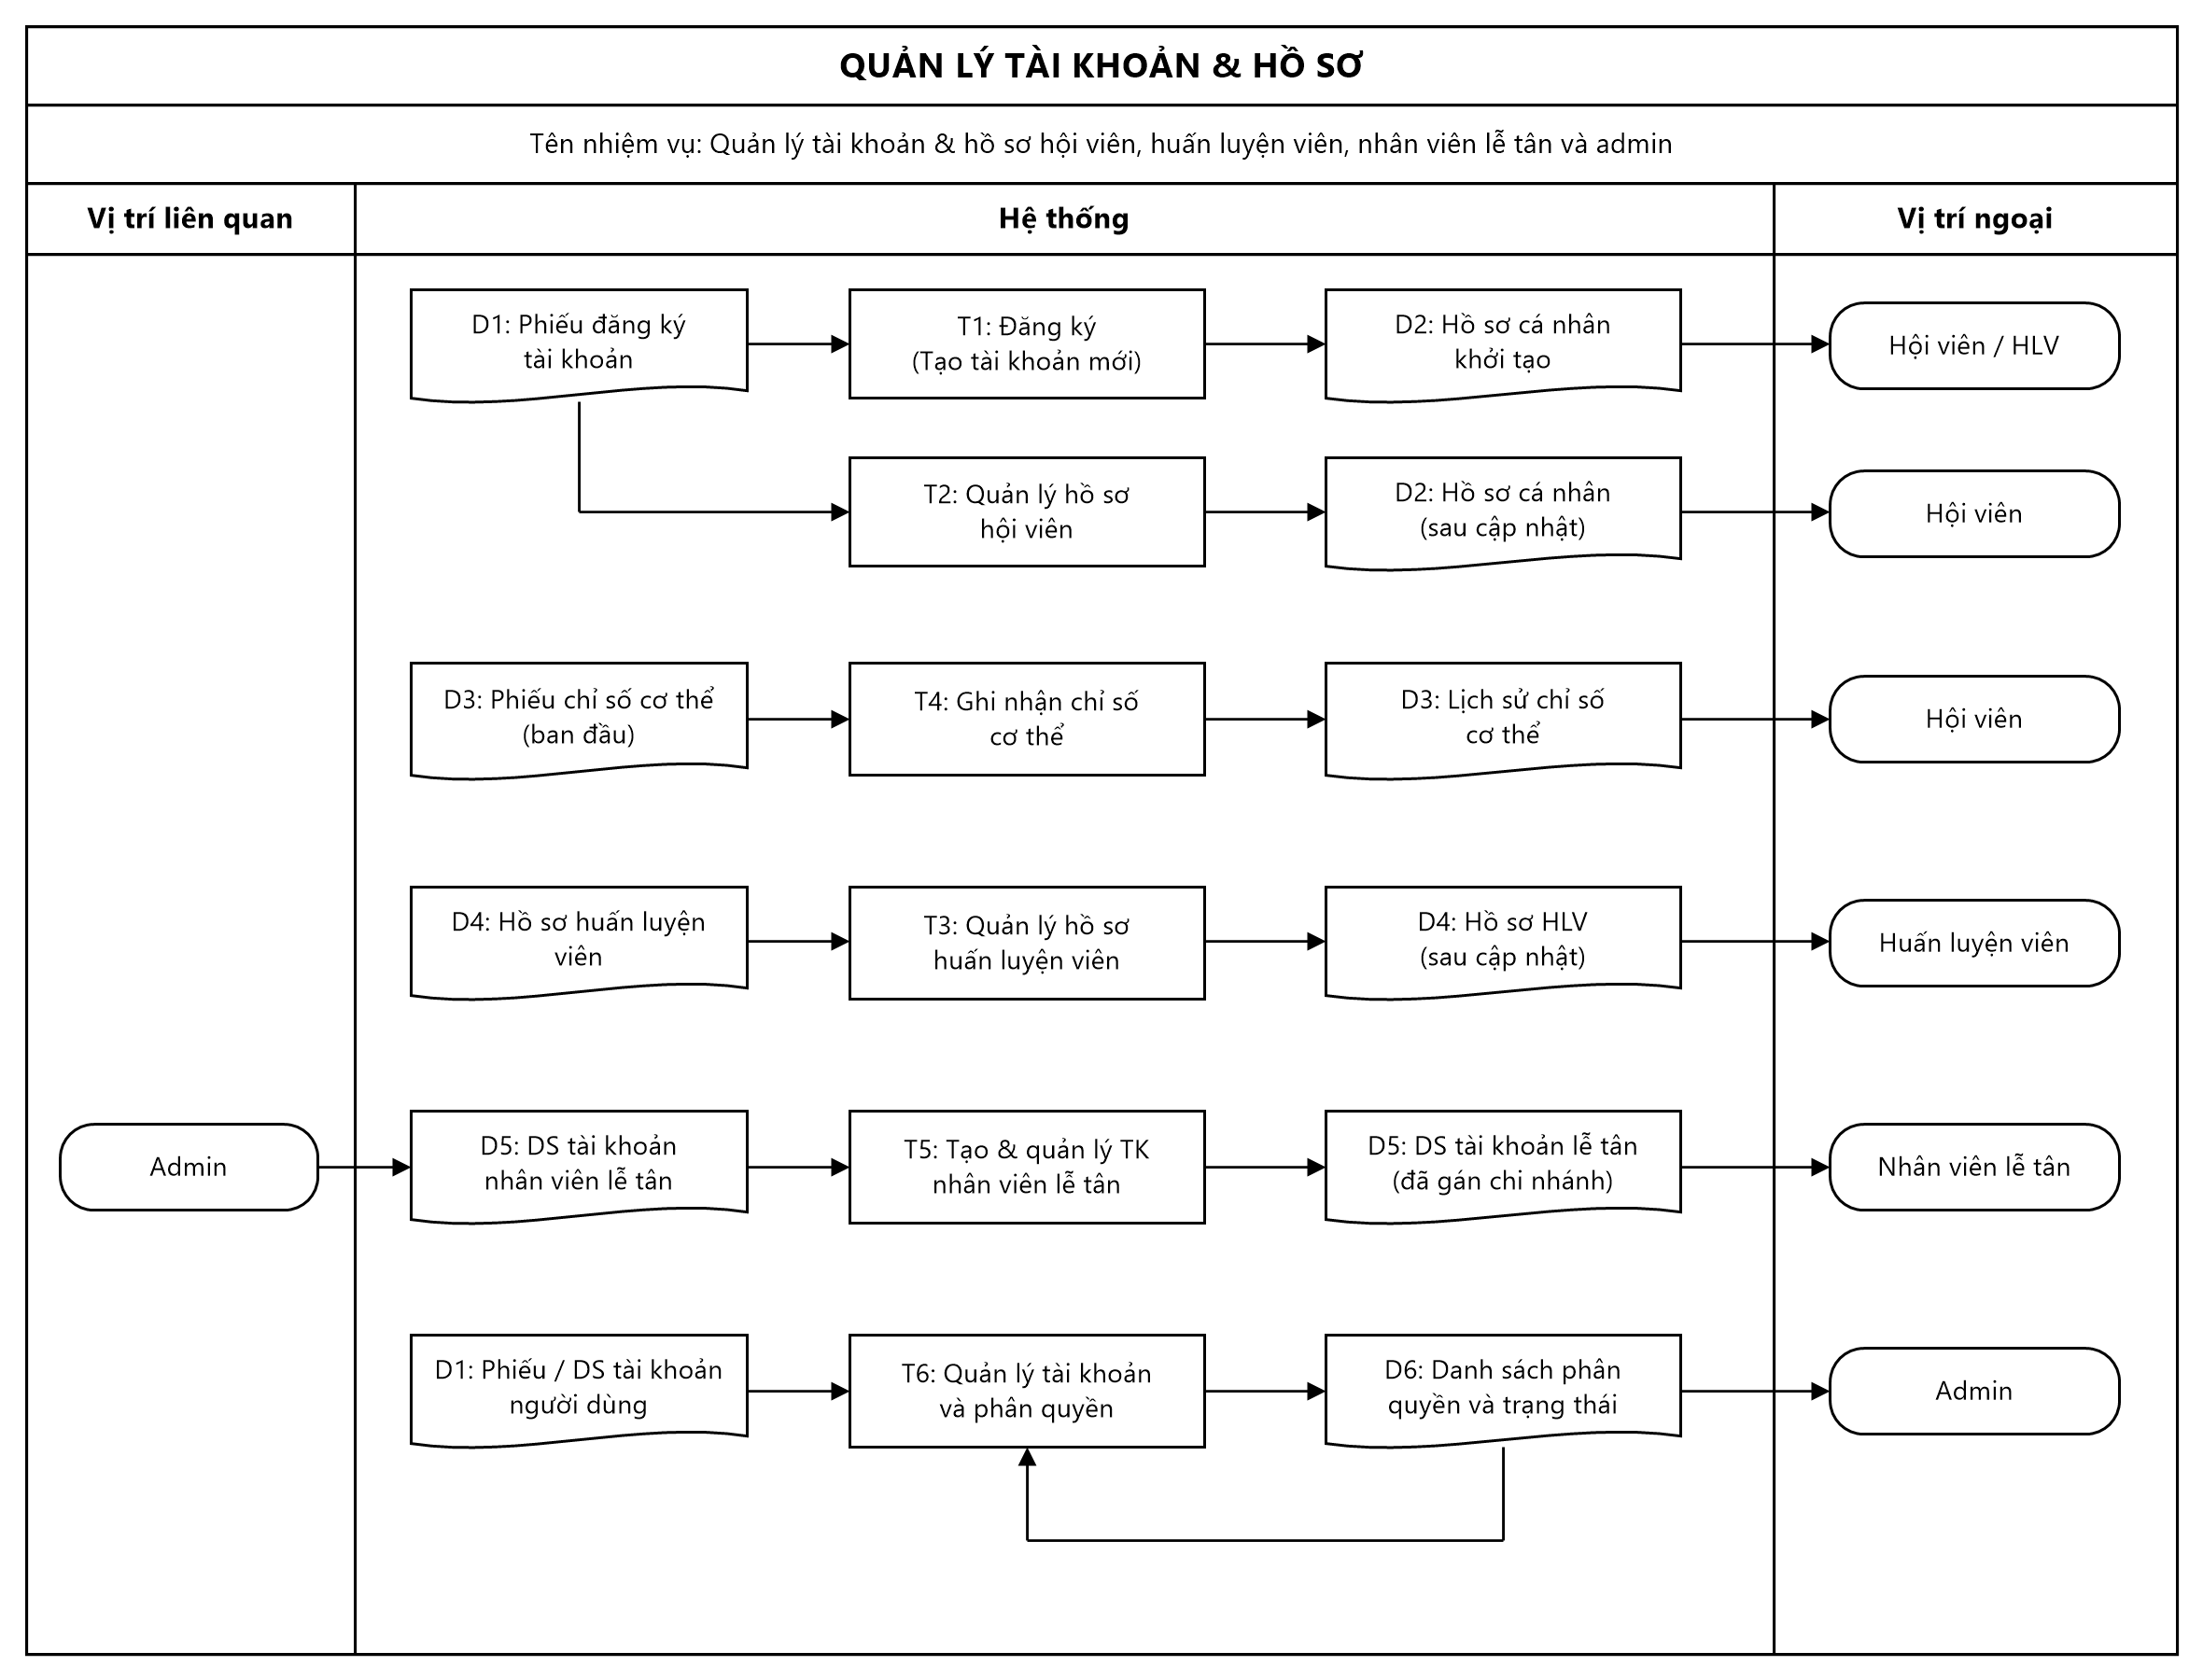
\includegraphics[width=0.92\textwidth, height=0.70\textheight, keepaspectratio]{images/ht_p06_1.png}
\caption{Sơ đồ hiện trạng 1: Quản lý Tài khoản \& Hồ sơ}
\end{figure}

\begin{longtable}{|c|L{1.3cm}|p{10.8cm}|L{1.8cm}|}
\hline \textbf{STT} & \textbf{Hồ sơ} & \textbf{Vai trò} & \textbf{Công việc} \\ \hline \endfirsthead
\hline \textbf{STT} & \textbf{Hồ sơ} & \textbf{Vai trò} & \textbf{Công việc} \\ \hline \endhead \hline \endfoot
\hline
\caption{Mô tả hồ sơ -- Quản lý Tài khoản \& Hồ sơ} \\
\endlastfoot
1 & D1 & Phiếu đăng ký tài khoản: dùng để Hội viên/PT đăng ký thông tin ban đầu (email, số điện thoại...). & T1 \\ \hline
2 & D2 & Hồ sơ cá nhân của hội viên: lưu thông tin cá nhân (ngày sinh, giới tính, địa chỉ) do hội viên cập nhật sau khi đăng ký. & T2 \\ \hline
3 & D3 & Phiếu chỉ số cơ thể ban đầu: ghi nhận sau lần đo đầu tiên (cân nặng, chiều cao, BMI...) làm mốc theo dõi tiến độ. & T4 \\ \hline
4 & D4 & Hồ sơ của huấn luyện viên: ghi nhận kinh nghiệm, chuyên môn, chi nhánh làm việc do HLV khai báo và cập nhật. & T3 \\ \hline
5 & D5 & Danh sách tài khoản nhân viên lễ tân: do Admin tạo, gán chi nhánh làm việc cho từng nhân viên. & T5 \\ \hline
6 & D6 & Danh sách phân quyền và trạng thái tài khoản: tổng hợp toàn bộ tài khoản để Admin quản lý truy cập và khóa/mở khóa. & T6 \\ \hline
\end{longtable}

{\setlength{\tabcolsep}{4pt}
\begin{longtable}{|L{0.9cm}|L{4.0cm}|L{2.5cm}|L{2.9cm}|L{1.7cm}|L{1.4cm}|L{1.4cm}|}
\hline \textbf{Mã} & \textbf{Mô tả công việc} & \textbf{Điều kiện khởi động} & \textbf{Quy tắc} & \textbf{Vị trí} & \textbf{Nhập} & \textbf{Xuất} \\ \hline \endfirsthead
\hline \textbf{Mã} & \textbf{Mô tả công việc} & \textbf{Điều kiện khởi động} & \textbf{Quy tắc} & \textbf{Vị trí} & \textbf{Nhập} & \textbf{Xuất} \\ \hline \endhead \hline \endfoot
\hline
\caption{Mô tả công việc -- Quản lý Tài khoản \& Hồ sơ} \\
\endlastfoot
T1 & Đăng ký: Hội viên hoặc HLV điền thông tin (email, mật khẩu, họ tên, SĐT) tạo tài khoản mới. & Người dùng chưa có tài khoản, truy cập trang đăng ký. & Email phải duy nhất; mật khẩu đạt độ an toàn tối thiểu. & Người dùng & Dữ liệu nhập & D1, D2 \\ \hline
T2 & Quản lý hồ sơ hội viên: Cập nhật thông tin cá nhân mở rộng của hội viên. & Hội viên đã có tài khoản và đăng nhập thành công. & Phải đăng ký và đăng nhập thành công. & Người dùng & D1 & D2 \\ \hline
T3 & Quản lý hồ sơ HLV: Khai báo/cập nhật chuyên môn, kinh nghiệm và chi nhánh làm việc. & HLV có tài khoản trên hệ thống. & Thông tin chuyên môn đầy đủ; hồ sơ PT mới phải được Admin duyệt. & Huấn luyện viên & D4 & D4 \\ \hline
T4 & Ghi nhận chỉ số cơ thể: Hội viên nhập cân nặng, chiều cao, BMI, tỷ lệ mỡ, khối lượng cơ. & Hội viên đã đăng nhập và có hồ sơ cá nhân. & Lần đo đầu tiên lưu làm mốc ban đầu; các lần sau lưu thành lịch sử đo. & Hội viên & D3 & D3 \\ \hline
T5 & Tạo \& quản lý tài khoản lễ tân: Admin tạo tài khoản lễ tân và gán chi nhánh làm việc. & Có nhu cầu bổ sung/thay đổi nhân viên lễ tân. & Mỗi nhân viên phải gán chi nhánh; vai trò \texttt{Staff} (Lễ tân). & Admin & D5 & D5 \\* \hline
T6 & Quản lý tài khoản và phân quyền: Admin xem, cập nhật vai trò, khóa hoặc mở khóa tài khoản. & Người dùng đã tồn tại trong hệ thống. & Chỉ Admin có quyền quản lý; tài khoản bị khóa không được đăng nhập. & Admin & D1 & D6 \\ \hline
\end{longtable}
}

\subsubsection{Sơ đồ hiện trạng 2: Membership \& Thanh toán}
\begin{figure}[H]
\centering
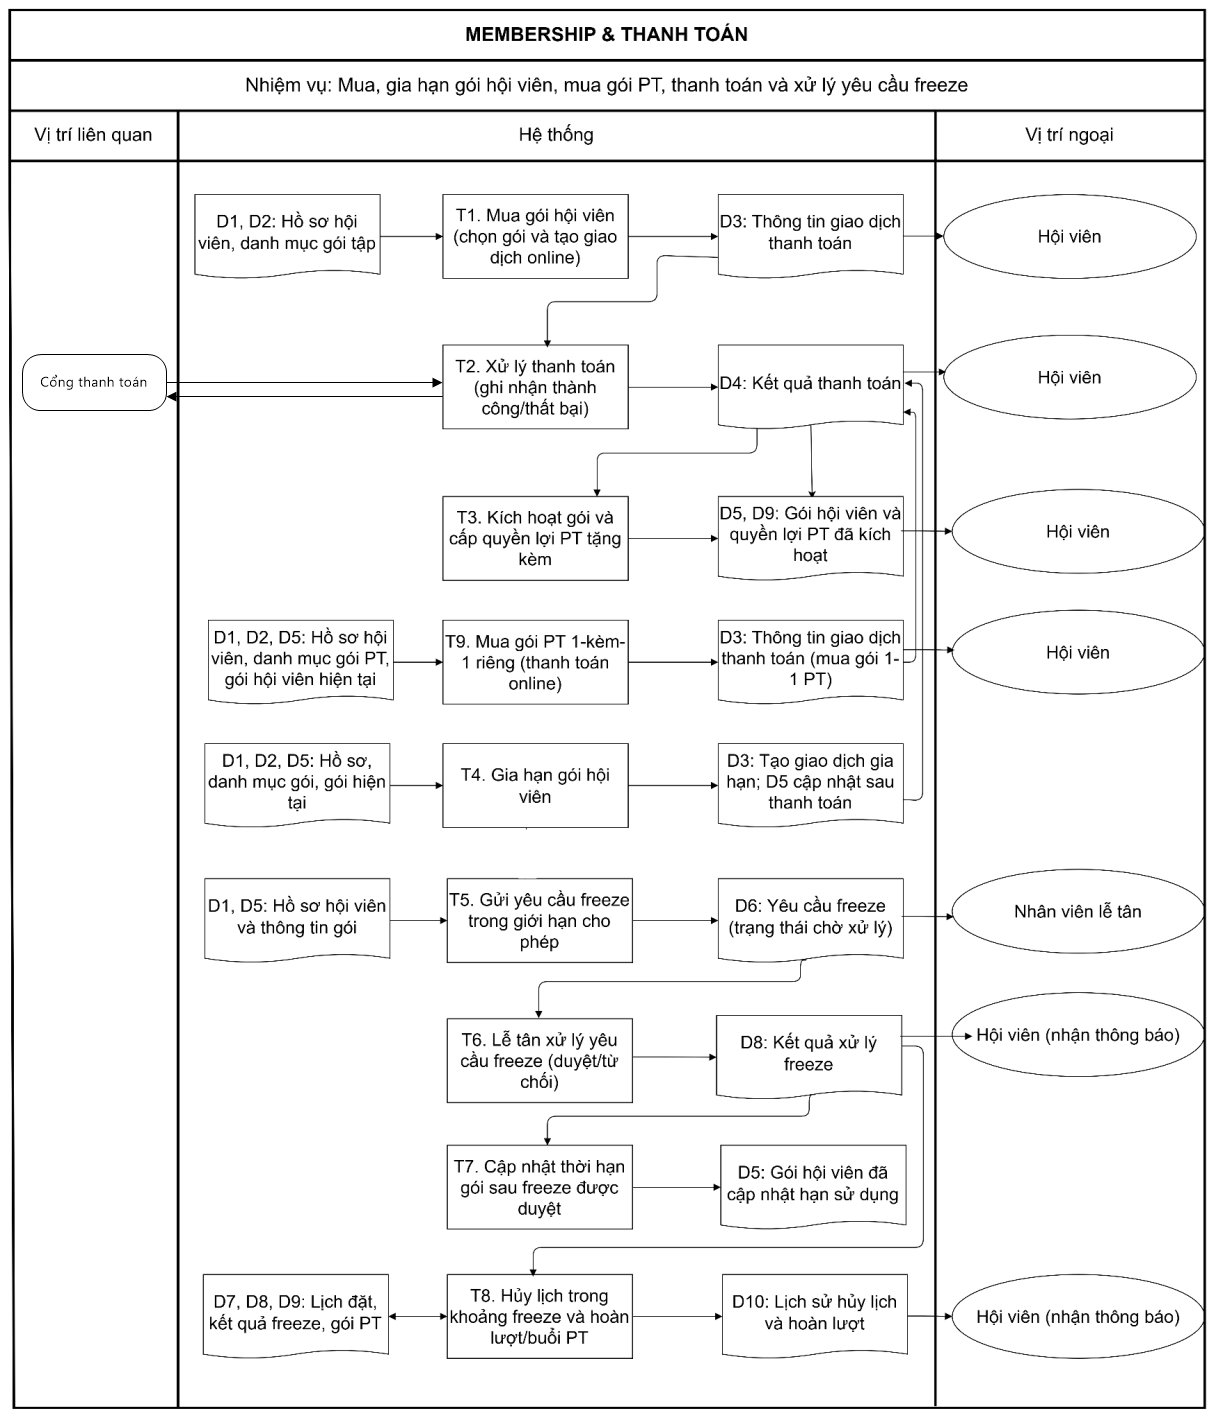
\includegraphics[width=0.92\textwidth, height=0.70\textheight, keepaspectratio]{images/ht_p10_1.png}
\caption{Sơ đồ hiện trạng 2: Membership \& Thanh toán}
\end{figure}

\begin{longtable}{|c|L{1.3cm}|p{10.6cm}|L{2.0cm}|}
\hline \textbf{STT} & \textbf{Hồ sơ} & \textbf{Vai trò} & \textbf{Công việc} \\ \hline \endfirsthead
\hline \textbf{STT} & \textbf{Hồ sơ} & \textbf{Vai trò} & \textbf{Công việc} \\ \hline \endhead \hline \endfoot
\hline
\caption{Mô tả hồ sơ -- Membership \& Thanh toán} \\
\endlastfoot
1 & D1 & Hồ sơ hội viên: cung cấp thông tin xác định hội viên thực hiện giao dịch. & T1, T4, T5, T9 \\ \hline
2 & D2 & Danh sách gói tập: cung cấp thông tin các gói đang bán, thời hạn, giá và quyền lợi. & T1, T4, T9 \\ \hline
3 & D3 & Thông tin giao dịch thanh toán: ghi nhận giao dịch mua/gia hạn, số tiền, phương thức và mã giao dịch. & T1, T2, T4, T9 \\ \hline
4 & D4 & Kết quả thanh toán: ghi nhận trạng thái thanh toán thành công hoặc thất bại. & T2, T3 \\ \hline
5 & D5 & Thông tin gói tập của hội viên: ngày bắt đầu, ngày hết hạn, trạng thái và quyền lợi còn lại. & T3, T4, T5, T7 \\ \hline
6 & D6 & Thông tin yêu cầu freeze: khoảng thời gian tạm ngưng, lý do và trạng thái chờ xử lý. & T5, T6 \\ \hline
7 & D7 & Thông tin lịch đặt tập: mã lịch, loại lịch, thời gian tập để xác định lịch bị ảnh hưởng bởi freeze. & T8 \\ \hline
8 & D8 & Kết quả xử lý freeze: trạng thái duyệt/từ chối, người xử lý, số ngày freeze được chấp nhận. & T6, T7, T8 \\ \hline
9 & D9 & Thông tin gói PT của hội viên: nguồn cấp (mua riêng hoặc tặng kèm), tổng buổi, đã dùng, còn lại. & T3, T8, T9 \\ \hline
10 & D10 & Kết quả hủy lịch: ghi nhận các lịch bị hủy do freeze và số lượt được hoàn lại. & T8 \\ \hline
\end{longtable}

{\setlength{\tabcolsep}{4pt}
\begin{longtable}{|L{0.9cm}|L{4.0cm}|L{2.5cm}|L{2.9cm}|L{1.7cm}|L{1.4cm}|L{1.4cm}|}
\hline \textbf{Mã} & \textbf{Mô tả công việc} & \textbf{Điều kiện khởi động} & \textbf{Quy tắc} & \textbf{Vị trí} & \textbf{Nhập} & \textbf{Xuất} \\ \hline \endfirsthead
\hline \textbf{Mã} & \textbf{Mô tả công việc} & \textbf{Điều kiện khởi động} & \textbf{Quy tắc} & \textbf{Vị trí} & \textbf{Nhập} & \textbf{Xuất} \\ \hline \endhead \hline \endfoot
\hline
\caption{Mô tả công việc -- Membership \& Thanh toán} \\
\endlastfoot
T1 & Mua gói tập: Hội viên chọn gói theo tháng/quý/năm và thực hiện thanh toán online. & Hội viên đã đăng nhập, muốn mua gói mới. & Gói phải còn hiệu lực bán, số tiền đúng giá gói. & Hội viên & D1, D2 & D3 \\ \hline
T2 & Xử lý thanh toán: Hệ thống tiếp nhận kết quả từ cổng thanh toán, ghi nhận giao dịch. & Hội viên thực hiện thanh toán gói tập. & Chỉ giao dịch thành công mới được kích hoạt gói. & Hệ thống / Cổng thanh toán & D3 & D3, D4 \\ \hline
T3 & Kích hoạt gói tập: Kích hoạt gói khi thanh toán thành công; nếu thất bại cho thanh toán lại. & Giao dịch có kết quả thanh toán thành công. & Chỉ kích hoạt khi thanh toán thành công. & Hệ thống & D4 & D5, D9 \\ \hline
T4 & Gia hạn gói tập: Gia hạn nối tiếp từ ngày hết hạn của gói hiện tại. & Hội viên có gói đang hoặc sắp hết hạn. & Ngày bắt đầu gói mới bằng ngày kết thúc gói hiện tại. & Hội viên & D1, D2, D5 & D3, D5 \\ \hline
T5 & Gửi yêu cầu freeze: Hội viên gửi đơn tạm ngưng gói trong giới hạn cho phép. & Gói đang hiệu lực và chưa vượt giới hạn freeze. & Không vượt quá số lần và số ngày freeze tối đa của gói. & Hội viên & D5, D1 & D6 \\ \hline
T6 & Xử lý yêu cầu freeze: Lễ tân tiếp nhận, kiểm tra và duyệt/từ chối yêu cầu. & Có yêu cầu freeze trạng thái chờ xử lý. & Chỉ chấp thuận khi đáp ứng giới hạn freeze của gói. & Nhân viên lễ tân & D6, D5 & D8 \\ \hline
T7 & Cập nhật thời hạn gói sau freeze: Cộng số ngày freeze được duyệt vào thời hạn gói. & Yêu cầu freeze được lễ tân chấp thuận. & Chỉ cộng số ngày freeze sau khi yêu cầu được duyệt. & Hệ thống & D8 & D5, D9 \\ \hline
T8 & Hủy lịch trong thời gian freeze: Tự động hủy lịch nằm trong khoảng freeze và hoàn lượt. & Freeze được duyệt và có lịch đặt trùng thời gian. & Chỉ hủy lịch bị ảnh hưởng và hoàn lại lượt/buổi. & Hệ thống & D8, D7, D9 & D10 \\ \hline
T9 & Mua gói PT riêng: Hội viên chọn gói PT 1-kèm-1 theo số buổi và thanh toán online. & Hội viên có gói hội viên còn hiệu lực. & Hết hiệu lực khi hết buổi hoặc quá hạn; không áp dụng freeze. & Hội viên, Hệ thống & D1, D2, D5 & D3, D9 \\ \hline
\end{longtable}
}

\subsubsection{Sơ đồ hiện trạng 3: Nghiệp vụ Quản lý Lớp học}
\begin{figure}[H]
\centering
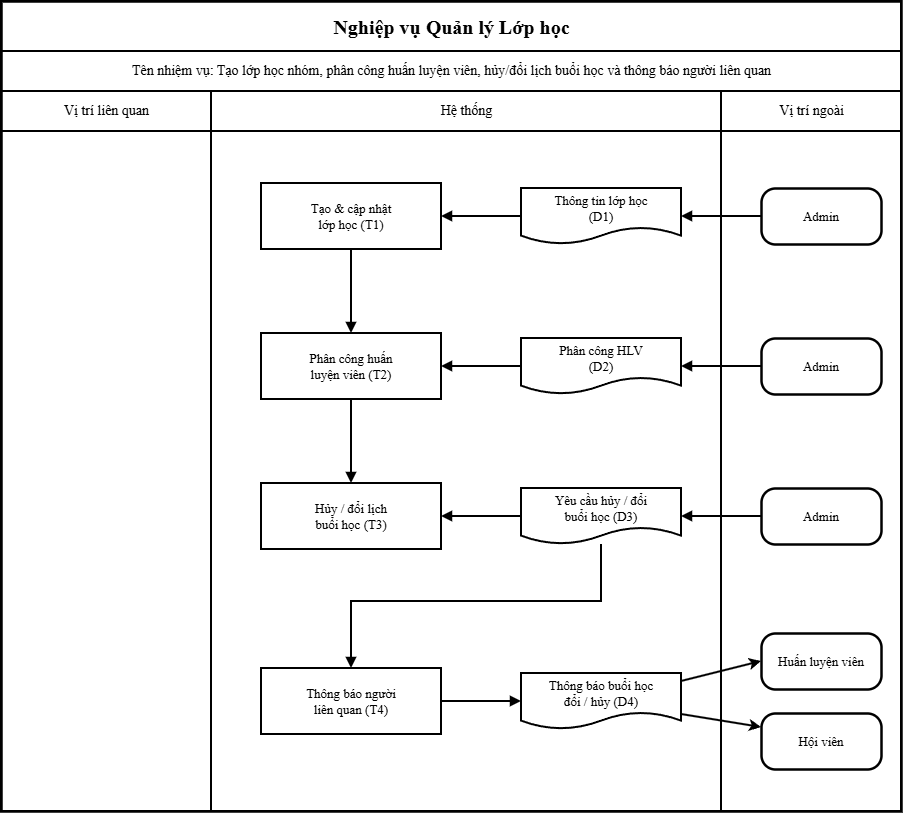
\includegraphics[width=0.88\textwidth, height=0.68\textheight, keepaspectratio]{images/ht_p19_1.png}
\caption{Sơ đồ hiện trạng 3: Nghiệp vụ Quản lý Lớp học}
\end{figure}

\begin{longtable}{|c|L{1.3cm}|p{10.8cm}|L{1.8cm}|}
\hline \textbf{STT} & \textbf{Hồ sơ} & \textbf{Vai trò} & \textbf{Công việc} \\ \hline \endfirsthead
\hline \textbf{STT} & \textbf{Hồ sơ} & \textbf{Vai trò} & \textbf{Công việc} \\ \hline \endhead \hline \endfoot
\hline
\caption{Mô tả hồ sơ -- Nghiệp vụ Quản lý Lớp học} \\
\endlastfoot
1 & D1 & Thông tin lớp học: chứa thông tin lớp học nhóm do Admin cung cấp phục vụ tạo/cập nhật lớp. & T1, T2 \\ \hline
2 & D2 & Phân công HLV: chứa thông tin phân công huấn luyện viên phụ trách lớp học. & T2, T3 \\ \hline
3 & D3 & Yêu cầu hủy / đổi buổi học: chứa thông tin yêu cầu hủy hoặc thay đổi lịch buổi học. & T3, T4 \\ \hline
4 & D4 & Thông báo buổi học đổi / hủy: chứa thông tin buổi học bị hủy/đổi lịch để gửi người liên quan. & T4 \\ \hline
\end{longtable}

{\setlength{\tabcolsep}{4pt}
\begin{longtable}{|L{0.9cm}|L{4.0cm}|L{2.5cm}|L{2.9cm}|L{1.7cm}|L{1.4cm}|L{1.4cm}|}
\hline \textbf{Mã} & \textbf{Mô tả công việc} & \textbf{Điều kiện khởi động} & \textbf{Quy tắc} & \textbf{Vị trí} & \textbf{Nhập} & \textbf{Xuất} \\ \hline \endfirsthead
\hline \textbf{Mã} & \textbf{Mô tả công việc} & \textbf{Điều kiện khởi động} & \textbf{Quy tắc} & \textbf{Vị trí} & \textbf{Nhập} & \textbf{Xuất} \\ \hline \endhead \hline \endfoot
\hline
\caption{Mô tả công việc -- Nghiệp vụ Quản lý Lớp học} \\
\endlastfoot
T1 & Tạo \& cập nhật lớp học: Tạo mới hoặc cập nhật thông tin lớp học nhóm theo thông tin Admin cung cấp. & Có thông tin lớp học cần tạo hoặc cập nhật. & Thông tin lớp học phải đầy đủ và hợp lệ. & Hệ thống & D1 & D1 \\ \hline
T2 & Phân công HLV: Phân công huấn luyện viên phụ trách lớp học dựa trên thông tin phân công. & Lớp học đã được tạo hoặc cập nhật. & HLV được phân công phải phù hợp với lớp học. & Hệ thống & D1, D2 & D2 \\ \hline
T3 & Hủy / đổi lịch buổi học: Tiếp nhận và thực hiện yêu cầu hủy hoặc thay đổi lịch buổi học. & Có yêu cầu hủy hoặc đổi lịch buổi học. & Chỉ thực hiện khi yêu cầu hợp lệ và cập nhật đúng thông tin buổi học. & Hệ thống & D2, D3 & D3 \\ \hline
T4 & Thông báo người liên quan: Tạo và gửi thông báo về buổi học bị hủy/đổi lịch đến HLV và hội viên. & Buổi học đã được hủy hoặc đổi lịch. & Thông báo phải gửi đúng HLV và hội viên liên quan. & Hệ thống & D3 & D4 \\ \hline
\end{longtable}
}

\subsubsection{Sơ đồ hiện trạng 4: Đặt lịch và Hủy lịch lớp nhóm}
\begin{figure}[H]
\centering
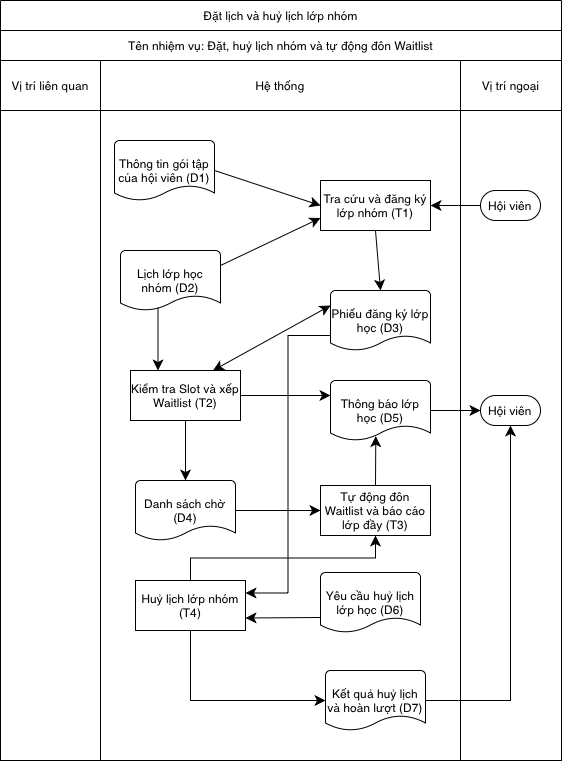
\includegraphics[width=0.82\textwidth, height=0.70\textheight, keepaspectratio]{images/ht_p24_1.png}
\caption{Sơ đồ hiện trạng 4: Đặt lịch và Hủy lịch lớp nhóm}
\end{figure}

\begin{longtable}{|c|L{1.3cm}|p{10.8cm}|L{1.8cm}|}
\hline \textbf{STT} & \textbf{Hồ sơ} & \textbf{Vai trò} & \textbf{Công việc} \\ \hline \endfirsthead
\hline \textbf{STT} & \textbf{Hồ sơ} & \textbf{Vai trò} & \textbf{Công việc} \\ \hline \endhead \hline \endfoot
\hline
\caption{Mô tả hồ sơ -- Đặt lịch và Hủy lịch lớp nhóm} \\
\endlastfoot
1 & D1 & Thông tin gói tập của Hội viên: trạng thái gói, số lượt còn lại. & T1 \\ \hline
2 & D2 & Lịch lớp học nhóm: tên lớp, HLV, chi nhánh, phòng tập, khung giờ, sĩ số tối đa. & T1, T2 \\ \hline
3 & D3 & Phiếu đăng ký lớp học: thông tin hội viên, mã lớp, thời gian đặt. & T1, T2 \\ \hline
4 & D4 & Danh sách chờ (Waitlist): thứ tự ưu tiên theo gói \& thời gian đăng ký. & T2, T3 \\ \hline
5 & D5 & Thông báo lớp học: thông báo đặt thành công, đôn lớp từ Waitlist, hoặc thông báo lớp đầy. & T2, T3 \\ \hline
6 & D6 & Yêu cầu hủy lịch lớp nhóm. & T4 \\ \hline
7 & D7 & Kết quả hủy lịch và Hoàn lượt: ghi nhận trạng thái hủy, hoàn lượt nếu đúng hạn. & T4 \\ \hline
\end{longtable}

{\setlength{\tabcolsep}{4pt}
\begin{longtable}{|L{0.9cm}|L{4.0cm}|L{2.5cm}|L{2.9cm}|L{1.7cm}|L{1.4cm}|L{1.4cm}|}
\hline \textbf{Mã} & \textbf{Mô tả công việc} & \textbf{Điều kiện khởi động} & \textbf{Quy tắc} & \textbf{Vị trí} & \textbf{Nhập} & \textbf{Xuất} \\ \hline \endfirsthead
\hline \textbf{Mã} & \textbf{Mô tả công việc} & \textbf{Điều kiện khởi động} & \textbf{Quy tắc} & \textbf{Vị trí} & \textbf{Nhập} & \textbf{Xuất} \\ \hline \endhead \hline \endfoot
\hline
\caption{Mô tả công việc -- Đặt lịch và Hủy lịch lớp nhóm} \\
\endlastfoot
T1 & Tra cứu và đăng ký lớp nhóm: Hội viên tra cứu lịch lớp theo khung giờ/chi nhánh và bấm đăng ký. & Hội viên truy cập tính năng đăng ký lớp nhóm. & Gói tập còn hiệu lực, chưa bị Freeze, còn lượt đặt, không trùng lịch. & Hội viên & D1, D2 & D3 \\ \hline
T2 & Kiểm tra Slot và xếp Waitlist: Nếu còn chỗ $\rightarrow$ đăng ký thành công; nếu đầy $\rightarrow$ đưa vào Waitlist. & Tiếp nhận yêu cầu đăng ký D3. & Waitlist sắp xếp theo độ ưu tiên gói (\texttt{VIP > Thường}) và thời điểm đăng ký. & Hệ thống & D2, D3 & D4, D5 \\ \hline
T3 & Tự động đôn Waitlist và báo lớp đầy: Có người hủy $\rightarrow$ đôn người cao nhất; mốc $T-8h$ $\rightarrow$ báo lớp đầy. & Có lượt hủy lớp hoặc đạt mốc $T-8h$ trước buổi học. & Chỉ đôn khi có người hủy; trước 8 giờ đóng hàng chờ và thông báo chọn lịch khác. & Hệ thống & D4 & D5 \\ \hline
T4 & Hủy lịch lớp nhóm: Hội viên gửi yêu cầu hủy lượt đặt. & Hội viên chọn hủy lịch trên ứng dụng. & Hủy đúng hạn $\rightarrow$ hoàn lượt; hủy quá hạn hoặc vắng mặt $\rightarrow$ tính đã sử dụng. & Hội viên & D6 & D7 \\ \hline
\end{longtable}
}

\subsubsection{Sơ đồ hiện trạng 5: Đặt lịch và Hủy lịch lớp PT kèm 1-1}
\begin{figure}[H]
\centering
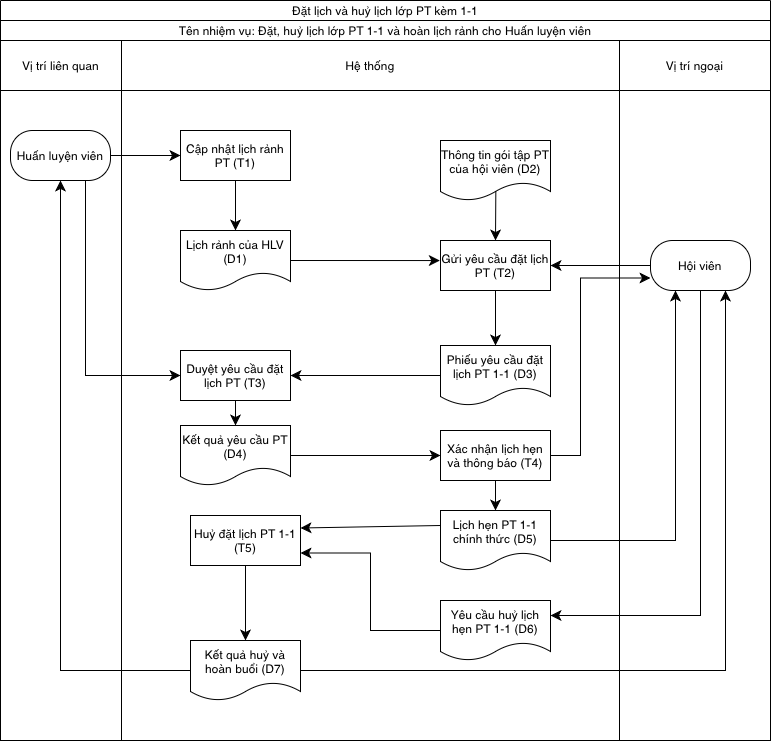
\includegraphics[width=0.88\textwidth, height=0.70\textheight, keepaspectratio]{images/ht_p28_1.png}
\caption{Sơ đồ hiện trạng 5: Đặt lịch và Hủy lịch lớp PT kèm 1-1}
\end{figure}

\begin{longtable}{|c|L{1.3cm}|p{10.8cm}|L{1.8cm}|}
\hline \textbf{STT} & \textbf{Hồ sơ} & \textbf{Vai trò} & \textbf{Công việc} \\ \hline \endfirsthead
\hline \textbf{STT} & \textbf{Hồ sơ} & \textbf{Vai trò} & \textbf{Công việc} \\ \hline \endhead \hline \endfoot
\hline
\caption{Mô tả hồ sơ -- Đặt lịch và Hủy lịch lớp PT kèm 1-1} \\
\endlastfoot
1 & D1 & Lịch rảnh của Huấn luyện viên: khung giờ rảnh, chi nhánh, chuyên môn. & T1, T2 \\ \hline
2 & D2 & Thông tin gói tập PT của Hội viên: số buổi 1-1 còn lại, thời hạn gói. & T2 \\ \hline
3 & D3 & Phiếu yêu cầu đặt lịch PT 1-1 (trạng thái: Chờ PT xác nhận). & T2, T3 \\ \hline
4 & D4 & Kết quả duyệt yêu cầu PT (Chấp nhận hoặc Từ chối từ PT). & T3, T4 \\ \hline
5 & D5 & Lịch hẹn PT 1-1 chính thức (trạng thái: Đã xác nhận / Đã xếp lịch). & T4, T5 \\ \hline
6 & D6 & Yêu cầu hủy lịch hẹn PT 1-1. & T5 \\* \hline
7 & D7 & Kết quả hủy và hoàn buổi PT (ghi nhận trạng thái hủy và cập nhật số buổi). & T5 \\ \hline
\end{longtable}

{\setlength{\tabcolsep}{4pt}
\begin{longtable}{|L{0.9cm}|L{4.0cm}|L{2.5cm}|L{2.9cm}|L{1.7cm}|L{1.4cm}|L{1.4cm}|}
\hline \textbf{Mã} & \textbf{Mô tả công việc} & \textbf{Điều kiện khởi động} & \textbf{Quy tắc} & \textbf{Vị trí} & \textbf{Nhập} & \textbf{Xuất} \\ \hline \endfirsthead
\hline \textbf{Mã} & \textbf{Mô tả công việc} & \textbf{Điều kiện khởi động} & \textbf{Quy tắc} & \textbf{Vị trí} & \textbf{Nhập} & \textbf{Xuất} \\ \hline \endhead \hline \endfoot
\hline
\caption{Mô tả công việc -- Đặt lịch và Hủy lịch lớp PT kèm 1-1} \\
\endlastfoot
T1 & Cập nhật lịch rảnh PT: HLV đăng nhập và cập nhật các khung giờ rảnh cá nhân. & PT có nhu cầu thiết lập/sửa lịch làm việc. & Lịch rảnh không trùng với lịch dạy các lớp học nhóm được phân công. & PT & -- & D1 \\ \hline
T2 & Gửi yêu cầu đặt lịch PT: Hội viên xem lịch rảnh, chọn khung giờ và gửi yêu cầu tập 1-1. & Hội viên chọn PT và khung giờ. & Gói PT còn hiệu lực, còn buổi khả dụng; không trùng lịch hẹn khác; tạm trừ 1 buổi PT (ưu tiên buổi tặng kèm trước). & Hội viên & D1, D2 & D3 \\ \hline
T3 & Duyệt yêu cầu đặt lịch PT: PT tiếp nhận thông báo và bấm Xác nhận hoặc Từ chối. & Có phiếu yêu cầu D3 gửi đến PT. & PT phải phản hồi trước thời gian hẹn. & PT & D3 & D4 \\ \hline
T4 & Xác nhận lịch hẹn \& Thông báo: Đồng ý $\rightarrow$ tạo lịch chính thức; từ chối $\rightarrow$ hoàn buổi và báo hội viên. & Tiếp nhận kết quả duyệt D4. & Đồng ý $\rightarrow$ khóa khung giờ PT \& xác nhận lịch chính thức; từ chối $\rightarrow$ hoàn lại 1 buổi PT đã tạm trừ \& mở lại khung giờ. & Hệ thống & D4 & D5 \\ \hline
T5 & Hủy lịch PT 1-1: Hội viên gửi yêu cầu hủy buổi tập đã xác nhận. & Có yêu cầu hủy từ Hội viên. & Hủy đúng hạn (trước $X$ giờ) $\rightarrow$ hoàn buổi; hủy quá hạn $\rightarrow$ tính đã sử dụng. & Hội viên / PT / Hệ thống & D5, D6 & D7 \\ \hline
\end{longtable}
}

\subsubsection{Sơ đồ hiện trạng 6: Check-in và Check-out}
\begin{figure}[H]
\centering
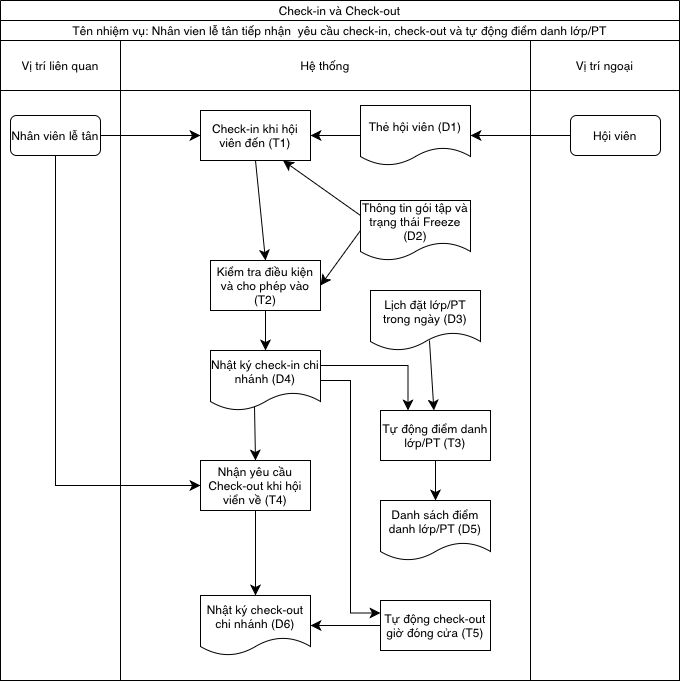
\includegraphics[width=0.86\textwidth, height=0.70\textheight, keepaspectratio]{images/ht_p34_1.png}
\caption{Sơ đồ hiện trạng 6: Check-in và Check-out}
\end{figure}

\begin{longtable}{|c|L{1.3cm}|p{10.8cm}|L{1.8cm}|}
\hline \textbf{STT} & \textbf{Hồ sơ} & \textbf{Vai trò} & \textbf{Công việc} \\ \hline \endfirsthead
\hline \textbf{STT} & \textbf{Hồ sơ} & \textbf{Vai trò} & \textbf{Công việc} \\ \hline \endhead \hline \endfoot
\hline
\caption{Mô tả hồ sơ -- Check-in và Check-out} \\
\endlastfoot
1 & D1 & Thẻ hội viên check-in. & T1 \\ \hline
2 & D2 & Thông tin gói tập và trạng thái Freeze: hiệu lực gói, ngày hết hạn, trạng thái tạm ngưng. & T2 \\ \hline
3 & D3 & Lịch đặt lớp / PT trong ngày: danh sách lịch học lớp nhóm và lịch PT đã xác nhận. & T3 \\ \hline
4 & D4 & Nhật ký Check-in chi nhánh: thời gian vào, mã chi nhánh, trạng thái hợp lệ. & T2, T3, T4, T5 \\ \hline
5 & D5 & Danh sách đánh dấu check-in Lớp / PT: ghi nhận hội viên đã có mặt tại chi nhánh để HLV xác nhận điểm danh. & T3 \\ \hline
6 & D6 & Nhật ký Check-out chi nhánh: thời gian ra, thời lượng tập, cập nhật số người tại phòng. & T4, T5 \\ \hline
\end{longtable}

{\setlength{\tabcolsep}{4pt}
\begin{longtable}{|L{0.9cm}|L{4.0cm}|L{2.5cm}|L{2.9cm}|L{1.7cm}|L{1.4cm}|L{1.4cm}|}
\hline \textbf{Mã} & \textbf{Mô tả công việc} & \textbf{Điều kiện khởi động} & \textbf{Quy tắc} & \textbf{Vị trí} & \textbf{Nhập} & \textbf{Xuất} \\ \hline \endfirsthead
\hline \textbf{Mã} & \textbf{Mô tả công việc} & \textbf{Điều kiện khởi động} & \textbf{Quy tắc} & \textbf{Vị trí} & \textbf{Nhập} & \textbf{Xuất} \\ \hline \endhead \hline \endfoot
\hline
\caption{Mô tả công việc -- Check-in và Check-out} \\
\endlastfoot
T1 & Check-in khi hội viên đến: Quét thẻ/QR hoặc lễ tân nhập thủ công thông tin thẻ hội viên. & Hội viên đến chi nhánh phòng gym. & Thẻ phải thuộc sở hữu của Hội viên và đọc được thiết bị (hoặc lễ tân xác minh). & Hội viên, Hệ thống & D1 & -- \\ \hline
T2 & Kiểm tra điều kiện và cho phép vào: Đối soát gói tập và Freeze; mở cửa nếu hợp lệ, báo lỗi nếu từ chối. & Hệ thống tiếp nhận yêu cầu check-in. & Gói còn hạn, không trong thời gian Freeze, đúng quyền lợi chi nhánh. & Hệ thống & D2 & D4 \\ \hline
T3 & Tự động đánh dấu check-in Lớp/PT: Nếu check-in thành công và có lịch lớp/PT trong ngày $\rightarrow$ đánh dấu cờ đã check-in làm cơ sở cho HLV điểm danh. & Check-in thành công. & Thời điểm check-in hợp lệ trong ngày diễn ra buổi học/PT tại đúng chi nhánh. & Hệ thống & D3, D4 & D5 \\ \hline
T4 & Nhận yêu cầu Check-out khi về: Hội viên quét thẻ hoặc báo lễ tân ghi nhận rời phòng gym. & Hội viên rời khỏi chi nhánh. & Hội viên phải đang có lượt check-in mở trong ngày. & Hội viên / Nhân viên lễ tân & D4 & D6 \\ \hline
T5 & Tự động Check-out giờ đóng cửa: Quét và đóng các lượt check-in chưa ra vào cuối ngày. & Đến giờ đóng cửa chi nhánh (22h00). & Mọi lượt check-in trong ngày chưa đóng sẽ tự động cập nhật giờ ra lúc đóng cửa. & Hệ thống & D4 & D6 \\ \hline
\end{longtable}
}

\subsubsection{Sơ đồ hiện trạng 7: Quản lý Lịch Nhân sự Chuyên môn (PT)}
Sơ đồ dưới đây trình bày quy trình nghiệp vụ theo góc nhìn vận hành của Huấn luyện viên (PT), bổ sung cho quy trình đặt/hủy lịch phía Hội viên ở Sơ đồ hiện trạng 5.
\begin{figure}[H]
\centering
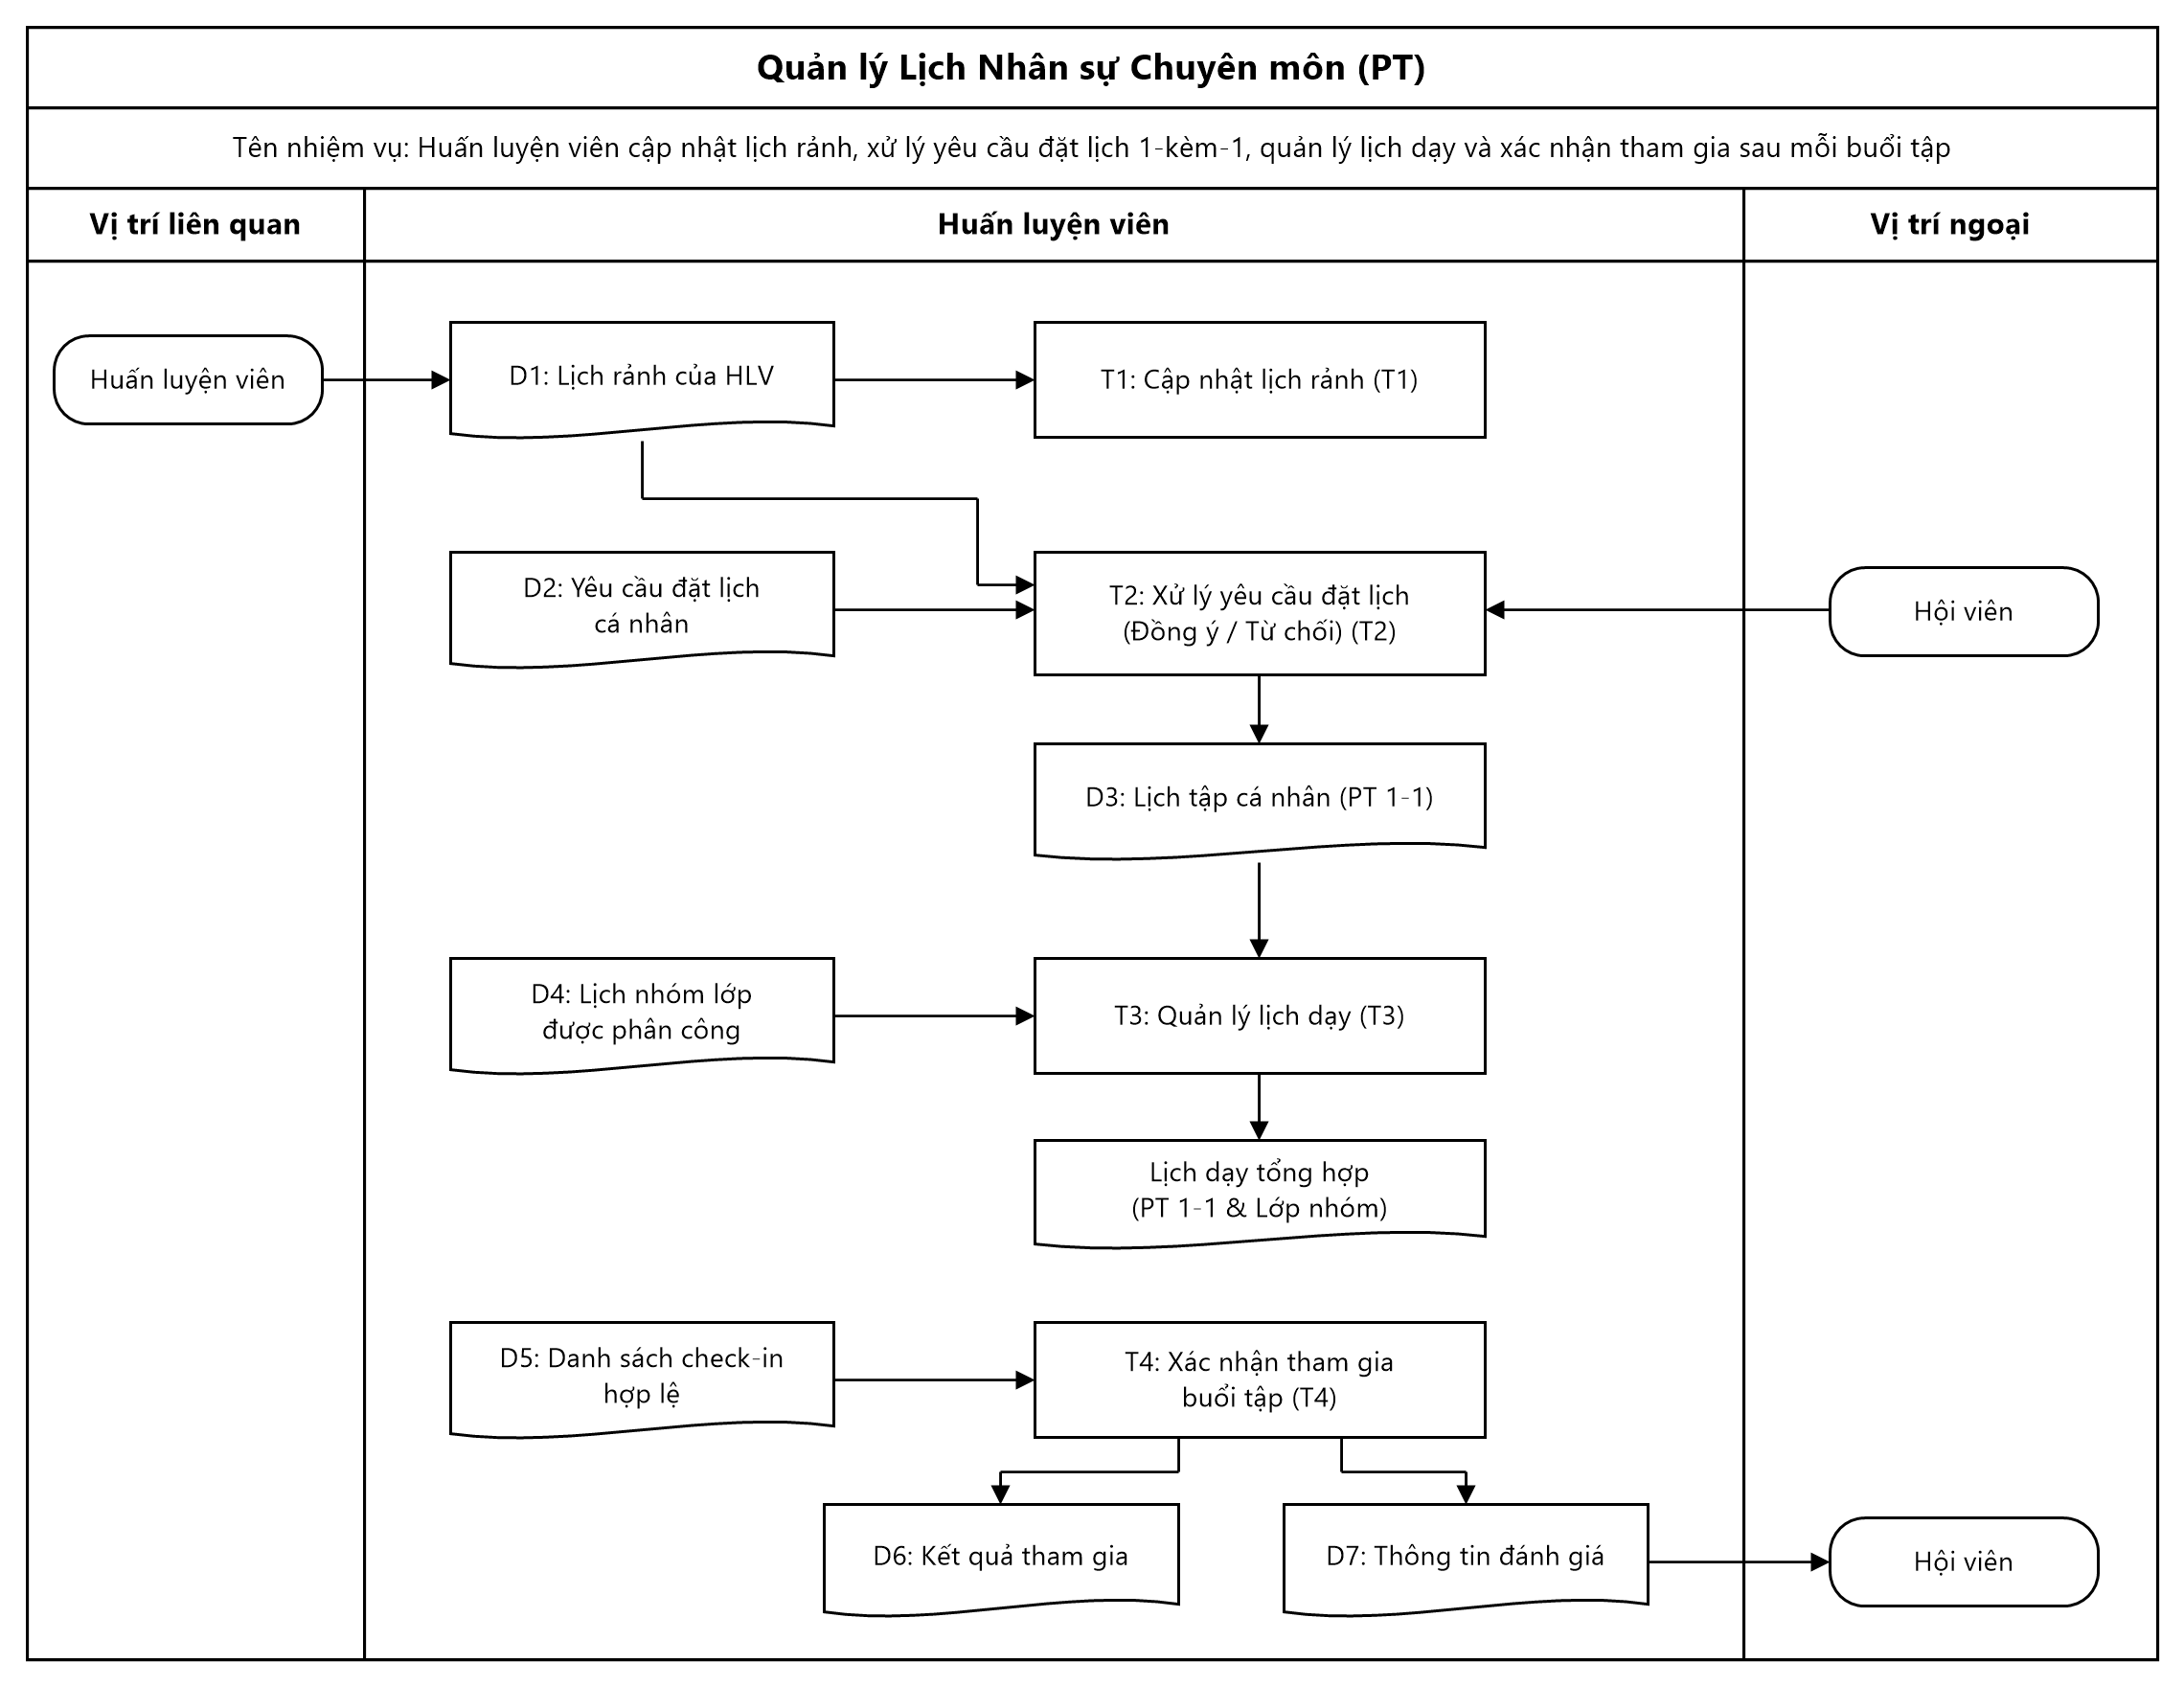
\includegraphics[width=0.88\textwidth, height=0.70\textheight, keepaspectratio]{images/ht_p39_1.png}
\caption{Sơ đồ hiện trạng 7: Quản lý Lịch Nhân sự Chuyên môn (PT)}
\end{figure}

\begin{longtable}{|c|L{1.3cm}|p{10.8cm}|L{1.8cm}|}
\hline \textbf{STT} & \textbf{Hồ sơ} & \textbf{Vai trò} & \textbf{Công việc} \\ \hline \endfirsthead
\hline \textbf{STT} & \textbf{Hồ sơ} & \textbf{Vai trò} & \textbf{Công việc} \\ \hline \endhead \hline \endfoot
\hline
\caption{Mô tả hồ sơ -- Quản lý Lịch Nhân sự Chuyên môn (PT)} \\
\endlastfoot
1 & D1 & Lịch rảnh của HLV: ghi nhận các khung thời gian HLV có thể nhận lịch tập cá nhân. & T1 \\ \hline
2 & D2 & Yêu cầu đặt lịch cá nhân: ghi nhận yêu cầu đặt lịch 1-kèm-1 của hội viên với HLV. & T2 \\ \hline
3 & D3 & Lịch tập cá nhân: ghi nhận các buổi tập 1-kèm-1 đã được HLV xác nhận. & T2, T3 \\ \hline
4 & D4 & Lịch lớp nhóm: ghi nhận các lớp nhóm và lịch dạy được phân công cho HLV. & T3 \\ \hline
5 & D5 & Danh sách check-in: ghi nhận hội viên đã check-in hợp lệ trước khi tham gia buổi tập. & T4 \\ \hline
6 & D6 & Kết quả tham gia: ghi nhận hội viên đã tham gia buổi tập sau khi HLV xác nhận. & T4 \\ \hline
7 & D7 & Thông tin đánh giá: khởi tạo quyền đánh giá cho hội viên sau khi xác nhận tham gia. & T4 \\ \hline
\end{longtable}

{\setlength{\tabcolsep}{4pt}
\begin{longtable}{|L{0.9cm}|L{4.0cm}|L{2.5cm}|L{2.9cm}|L{1.7cm}|L{1.4cm}|L{1.4cm}|}
\hline \textbf{Mã} & \textbf{Mô tả công việc} & \textbf{Điều kiện khởi động} & \textbf{Quy tắc} & \textbf{Vị trí} & \textbf{Nhập} & \textbf{Xuất} \\ \hline \endfirsthead
\hline \textbf{Mã} & \textbf{Mô tả công việc} & \textbf{Điều kiện khởi động} & \textbf{Quy tắc} & \textbf{Vị trí} & \textbf{Nhập} & \textbf{Xuất} \\ \hline \endhead \hline \endfoot
\hline
\caption{Mô tả công việc -- Quản lý Lịch Nhân sự Chuyên môn (PT)} \\
\endlastfoot
T1 & Cập nhật lịch rảnh: HLV cập nhật các khung thời gian có thể nhận lịch tập 1-kèm-1. & Khi HLV có hoặc thay đổi thời gian rảnh. & Chỉ cho phép đăng ký các khung giờ chưa bị trùng lịch. & HLV & D1 & D1 \\ \hline
T2 & Xử lý yêu cầu đặt lịch cá nhân: HLV xem yêu cầu đặt lịch 1-kèm-1 và xác nhận hoặc từ chối. & Khi hội viên gửi yêu cầu đặt lịch. & Không xác nhận lịch bị trùng hoặc ngoài thời gian rảnh. & HLV & D1, D2 & D3 \\ \hline
T3 & Quản lý lịch dạy: HLV theo dõi lịch tập cá nhân đã xác nhận và các lớp nhóm được phân công. & Khi có lịch xác nhận hoặc được phân công lớp. & Tổng hợp hiển thị lịch dạy cá nhân và lớp nhóm; không trùng lịch giữa các buổi/lớp. & HLV & D3, D4 & Lịch dạy tổng hợp \\ \hline
T4 & Xác nhận tham gia: Sau buổi tập, HLV kiểm tra danh sách check-in hợp lệ và xác nhận tham gia. & Sau khi buổi tập kết thúc. & Chỉ xác nhận hội viên có check-in hợp lệ. & HLV & D5 & D6, D7 \\ \hline
\end{longtable}
}

\subsubsection{Sơ đồ hiện trạng 8: Theo dõi Tiến độ \& Đánh giá}
\begin{figure}[H]
\centering
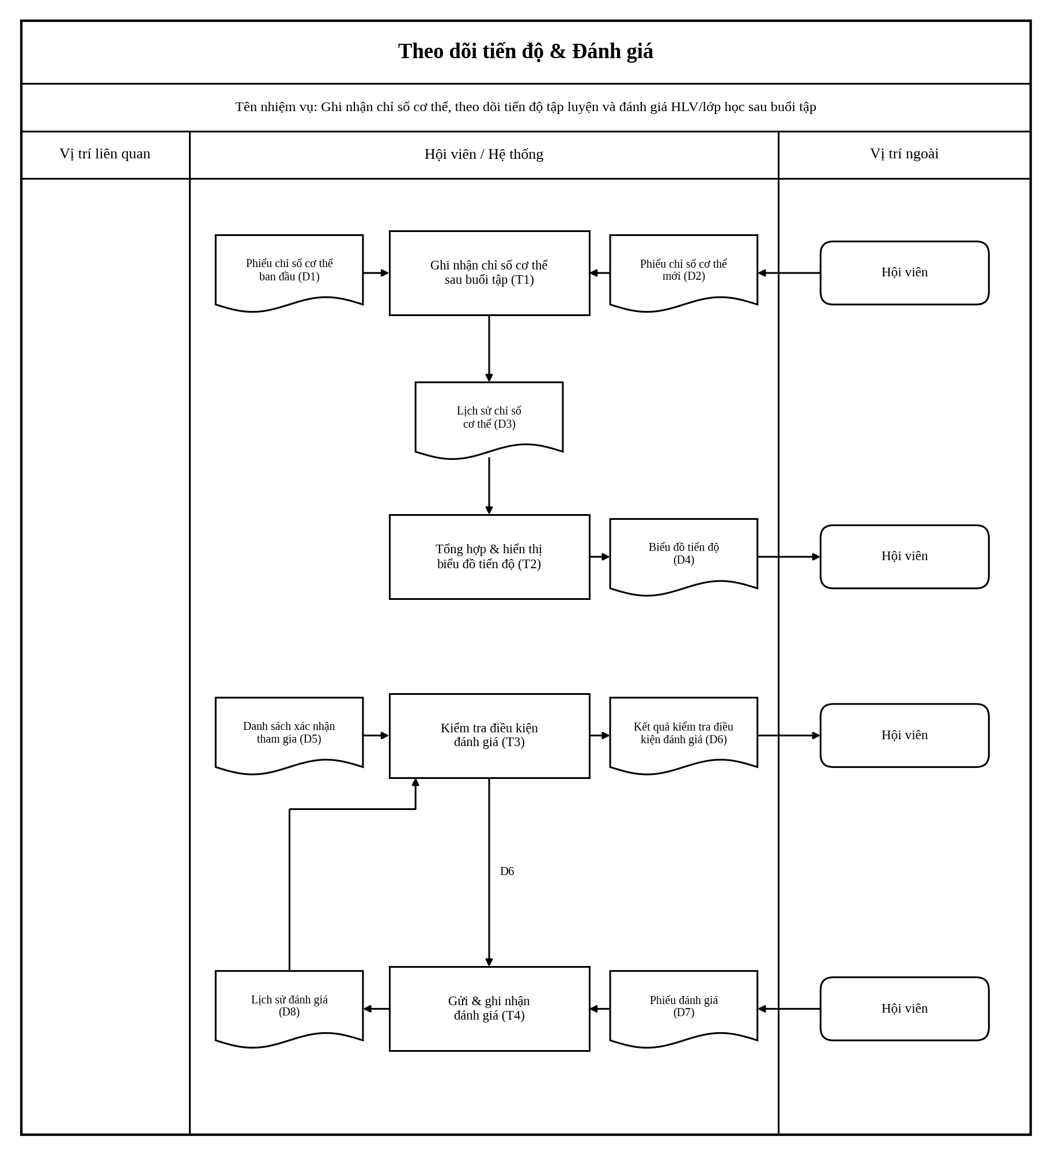
\includegraphics[width=0.90\textwidth, height=0.70\textheight, keepaspectratio]{images/ht_p44_1.png}
\caption{Sơ đồ hiện trạng 8: Theo dõi Tiến độ \& Đánh giá}
\end{figure}

\begin{longtable}{|c|L{1.3cm}|p{10.8cm}|L{1.8cm}|}
\hline \textbf{STT} & \textbf{Hồ sơ} & \textbf{Vai trò} & \textbf{Công việc} \\ \hline \endfirsthead
\hline \textbf{STT} & \textbf{Hồ sơ} & \textbf{Vai trò} & \textbf{Công việc} \\ \hline \endhead \hline \endfoot
\hline
\caption{Mô tả hồ sơ -- Theo dõi Tiến độ \& Đánh giá} \\
\endlastfoot
1 & D1 & Phiếu chỉ số cơ thể ban đầu: chỉ số lần đo đầu tiên, lưu làm mốc theo dõi tiến độ. & T1 \\ \hline
2 & D2 & Phiếu chỉ số cơ thể mới: các chỉ số hội viên nhập sau buổi tập, kèm thời điểm đo. & T1 \\ \hline
3 & D3 & Lịch sử chỉ số cơ thể: toàn bộ các lần đo theo thời gian (gồm mốc ban đầu và các lần sau). & T1, T2 \\ \hline
4 & D4 & Biểu đồ tiến độ: dữ liệu tổng hợp từ lịch sử đo để xem sự thay đổi theo thời gian. & T2 \\ \hline
5 & D5 & Danh sách xác nhận tham gia: các buổi lớp nhóm/PT 1-1 đã xác nhận tham gia (kèm check-in). & T3 \\ \hline
6 & D6 & Kết quả kiểm tra điều kiện đánh giá: cho phép hoặc từ chối đánh giá kèm lý do. & T3, T4 \\ \hline
7 & D7 & Phiếu đánh giá: đánh giá của hội viên về HLV/lớp học (điểm và nhận xét). & T4 \\ \hline
8 & D8 & Lịch sử đánh giá: các đánh giá đã ghi nhận, dùng kiểm tra đánh giá trùng và làm đầu vào báo cáo. & T3, T4 \\ \hline
\end{longtable}

{\setlength{\tabcolsep}{4pt}
\begin{longtable}{|L{0.9cm}|L{4.0cm}|L{2.5cm}|L{2.9cm}|L{1.7cm}|L{1.4cm}|L{1.4cm}|}
\hline \textbf{Mã} & \textbf{Mô tả công việc} & \textbf{Điều kiện khởi động} & \textbf{Quy tắc} & \textbf{Vị trí} & \textbf{Nhập} & \textbf{Xuất} \\ \hline \endfirsthead
\hline \textbf{Mã} & \textbf{Mô tả công việc} & \textbf{Điều kiện khởi động} & \textbf{Quy tắc} & \textbf{Vị trí} & \textbf{Nhập} & \textbf{Xuất} \\ \hline \endhead \hline \endfoot
\hline
\caption{Mô tả công việc -- Theo dõi Tiến độ \& Đánh giá} \\
\endlastfoot
T1 & Ghi nhận chỉ số cơ thể sau buổi tập: Nhập cân nặng, chiều cao, BMI, tỷ lệ mỡ, khối lượng cơ. & Hội viên đã đăng nhập, vừa kết thúc buổi tập. & Giá trị hợp lệ, lưu kèm thời điểm đo; lần đầu là mốc ban đầu không ghi đè. & Hội viên & D1, D2 & D3 \\ \hline
T2 & Tổng hợp \& hiển thị biểu đồ tiến độ: Lấy lịch sử đo và tổng hợp thành biểu đồ. & Hội viên yêu cầu xem tiến độ tập luyện. & Chỉ hiển thị dữ liệu của chính hội viên; lấy mốc ban đầu làm điểm so sánh. & Hệ thống & D3 & D4 \\ \hline
T3 & Kiểm tra điều kiện đánh giá: Kiểm tra buổi đã được xác nhận tham gia và chưa đánh giá. & Hội viên chọn đánh giá HLV/lớp sau buổi tập. & Chỉ cho đánh giá khi đã tham gia và mỗi buổi chỉ đánh giá một lần. & Hệ thống & D5, D8 & D6 \\* \hline
T4 & Gửi và ghi nhận đánh giá: Hội viên chấm điểm, nhận xét; hệ thống lưu gắn với buổi tương ứng. & Kết quả kiểm tra điều kiện cho phép đánh giá. & Điểm nằm trong thang quy định; sau khi lưu không được đánh giá lại buổi đó. & Hội viên & D6, D7 & D8 \\ \hline
\end{longtable}
}

\subsubsection{Sơ đồ hiện trạng 9: Quản lý Chi nhánh \& Thiết bị}
\begin{figure}[H]
\centering
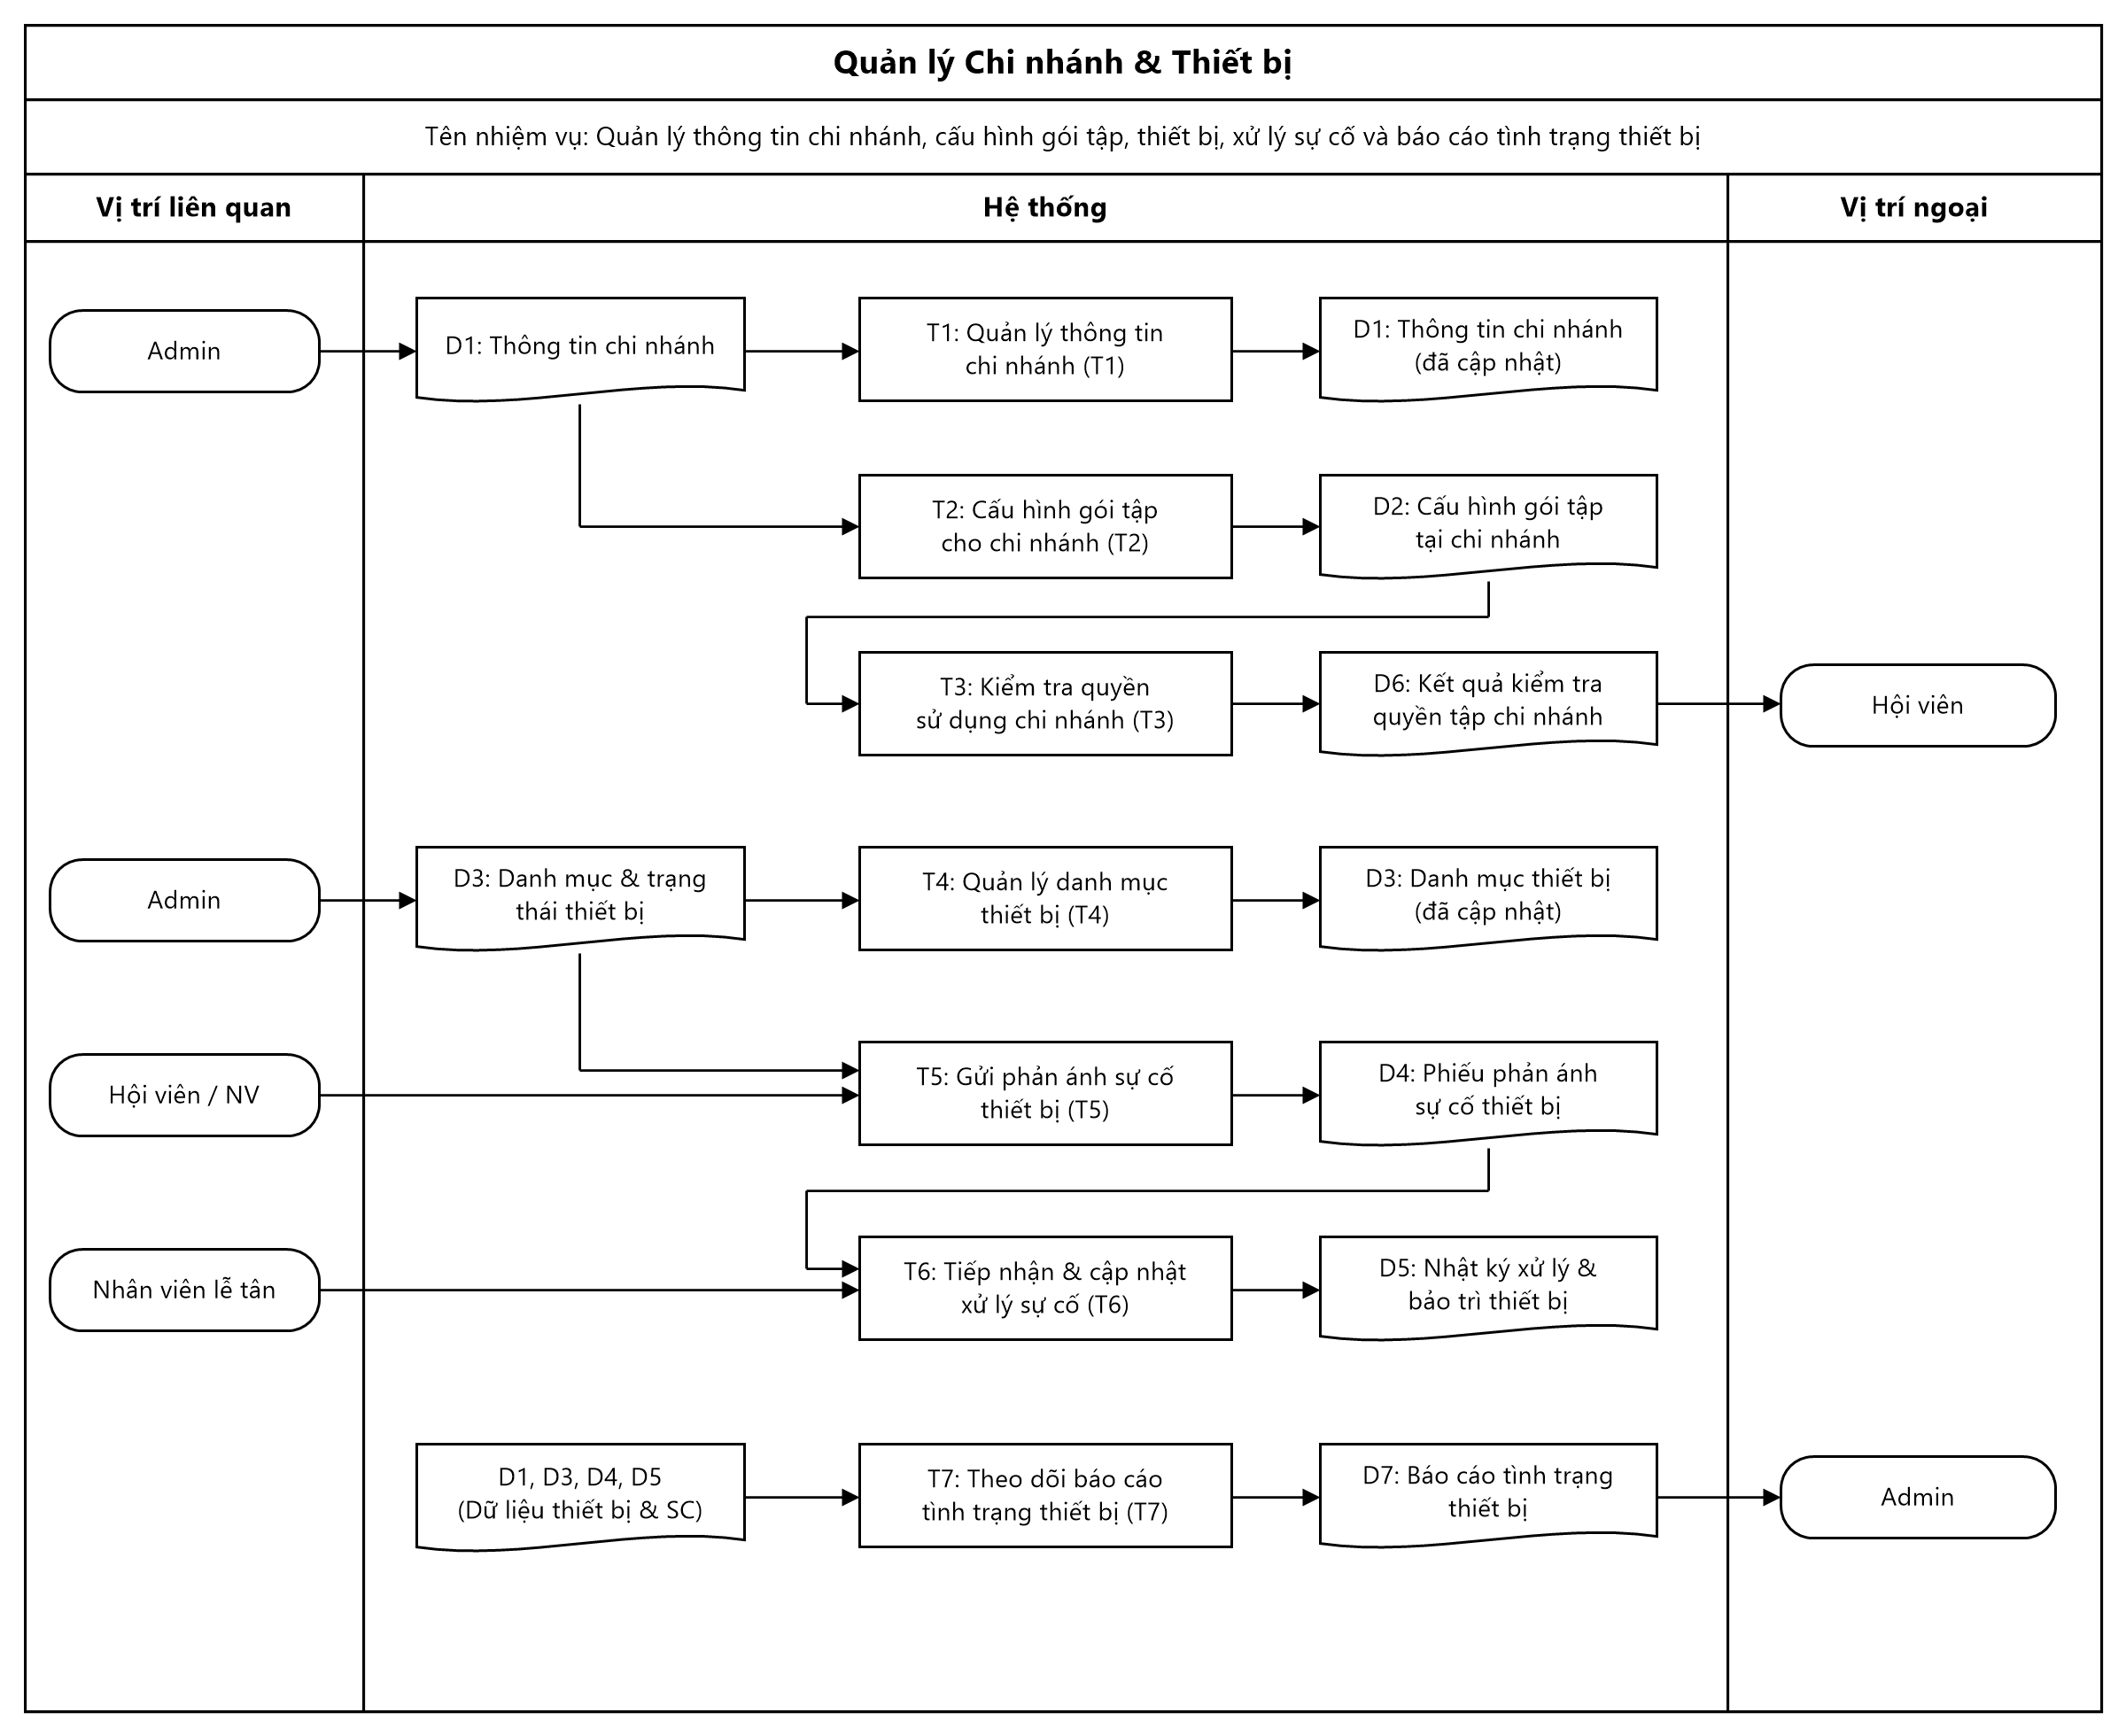
\includegraphics[width=0.92\textwidth, height=0.70\textheight, keepaspectratio]{images/ht_p51_1.png}
\caption{Sơ đồ hiện trạng 9: Quản lý Chi nhánh \& Thiết bị}
\end{figure}

\begin{longtable}{|c|L{1.3cm}|p{10.8cm}|L{1.8cm}|}
\hline \textbf{STT} & \textbf{Hồ sơ} & \textbf{Vai trò} & \textbf{Công việc} \\ \hline \endfirsthead
\hline \textbf{STT} & \textbf{Hồ sơ} & \textbf{Vai trò} & \textbf{Công việc} \\ \hline \endhead \hline \endfoot
\hline
\caption{Mô tả hồ sơ -- Quản lý Chi nhánh \& Thiết bị} \\
\endlastfoot
1 & D1 & Thông tin chi nhánh: lưu mã chi nhánh, tên, địa chỉ, số điện thoại, giờ mở/đóng cửa, trạng thái hoạt động. & T1, T2, T4, T7 \\ \hline
2 & D2 & Cấu hình gói tập tại chi nhánh: ghi nhận các gói áp dụng và phạm vi sử dụng tại từng chi nhánh. & T2, T3 \\ \hline
3 & D3 & Danh mục \& trạng thái thiết bị: ghi nhận mã máy, chi nhánh và tình trạng hiện tại (hoạt động, hỏng, đang sửa chữa, ngừng dùng). & T4, T5, T6, T7 \\ \hline
4 & D4 & Phiếu phản ánh sự cố thiết bị: ghi nhận phản ánh của Hội viên/Nhân viên kèm thời gian, ảnh và mô tả sự cố. & T5, T6, T7 \\ \hline
5 & D5 & Nhật ký xử lý \& bảo trì thiết bị: ghi nhận lịch sử tiếp nhận, quá trình sửa chữa và hoàn tất bảo trì của Lễ tân. & T6, T7 \\ \hline
6 & D6 & Kết quả kiểm tra quyền tập chi nhánh: kết quả cho phép hoặc từ chối truy cập chi nhánh khi check-in. & T3 \\ \hline
7 & D7 & Báo cáo tình trạng thiết bị: tổng hợp số lượng thiết bị theo trạng thái và lịch sử xử lý sự cố theo từng chi nhánh. & T7 \\ \hline
\end{longtable}

{\setlength{\tabcolsep}{4pt}
\begin{longtable}{|L{0.9cm}|L{4.0cm}|L{2.5cm}|L{2.9cm}|L{1.7cm}|L{1.4cm}|L{1.4cm}|}
\hline \textbf{Mã} & \textbf{Mô tả công việc} & \textbf{Điều kiện khởi động} & \textbf{Quy tắc} & \textbf{Vị trí} & \textbf{Nhập} & \textbf{Xuất} \\ \hline \endfirsthead
\hline \textbf{Mã} & \textbf{Mô tả công việc} & \textbf{Điều kiện khởi động} & \textbf{Quy tắc} & \textbf{Vị trí} & \textbf{Nhập} & \textbf{Xuất} \\ \hline \endhead \hline \endfoot
\hline
\caption{Mô tả công việc -- Quản lý Chi nhánh \& Thiết bị} \\
\endlastfoot
T1 & Quản lý thông tin chi nhánh: Admin thêm mới hoặc cập nhật thông tin chi nhánh. & Admin đăng nhập và có quyền quản lý chi nhánh. & Mã chi nhánh không trùng; chi nhánh ngừng hoạt động không nhận hoạt động mới. & Admin & D1 & D1 \\ \hline
T2 & Cấu hình gói tập cho chi nhánh: Thiết lập gói áp dụng chung hoặc riêng tại từng chi nhánh. & Chi nhánh và gói tập đã tồn tại trên hệ thống. & Chỉ áp dụng gói đang được phép sử dụng; không cấu hình trùng. & Admin & D1, D2 & D2 \\ \hline
T3 & Kiểm tra quyền sử dụng chi nhánh: Xác định hội viên có được phép check-in tại chi nhánh. & Hội viên có gói còn hiệu lực và thực hiện check-in tại chi nhánh. & Chỉ cho phép nếu gói còn hiệu lực và có quyền sử dụng chi nhánh đó. & Hệ thống & D2 & D6 \\ \hline
T4 & Quản lý danh mục thiết bị: Admin thêm mới, cập nhật thông tin hoặc ngừng sử dụng thiết bị theo chi nhánh. & Admin đăng nhập và chọn chi nhánh cần quản lý. & Mỗi thiết bị thuộc một chi nhánh; mã thiết bị không trùng. & Admin & D1, D3 & D3 \\ \hline
T5 & Gửi phản ánh sự cố thiết bị: Hội viên/Nhân viên gửi báo hỏng khi phát hiện thiết bị gặp sự cố. & Người dùng đang sử dụng dịch vụ hoặc làm việc tại chi nhánh. & Phản ánh phải xác định đúng thiết bị và nội dung sự cố. & Hội viên / Nhân viên & D3 & D4 \\ \hline
T6 & Tiếp nhận và xử lý sự cố: Lễ tân tiếp nhận phản ánh, cập nhật nhật ký sửa chữa và trạng thái thiết bị. & Có phản ánh sự cố thiết bị D4 ở trạng thái chờ xử lý. & Chỉ nhân viên được phân công tại chi nhánh mới được xử lý. & Nhân viên lễ tân & D3, D4 & D3, D5 \\ \hline
T7 & Theo dõi báo cáo tình trạng thiết bị: Admin xem tổng hợp tình trạng thiết bị và sự cố theo chi nhánh. & Hệ thống đã có dữ liệu thiết bị và lịch sử xử lý. & Báo cáo phản ánh đúng trạng thái hiện tại, lọc theo chi nhánh. & Admin & D1, D3, D4, D5 & D7 \\ \hline
\end{longtable}
}

\subsubsection{Sơ đồ hiện trạng 10: Báo cáo \& Thống kê}
\begin{figure}[H]
\centering
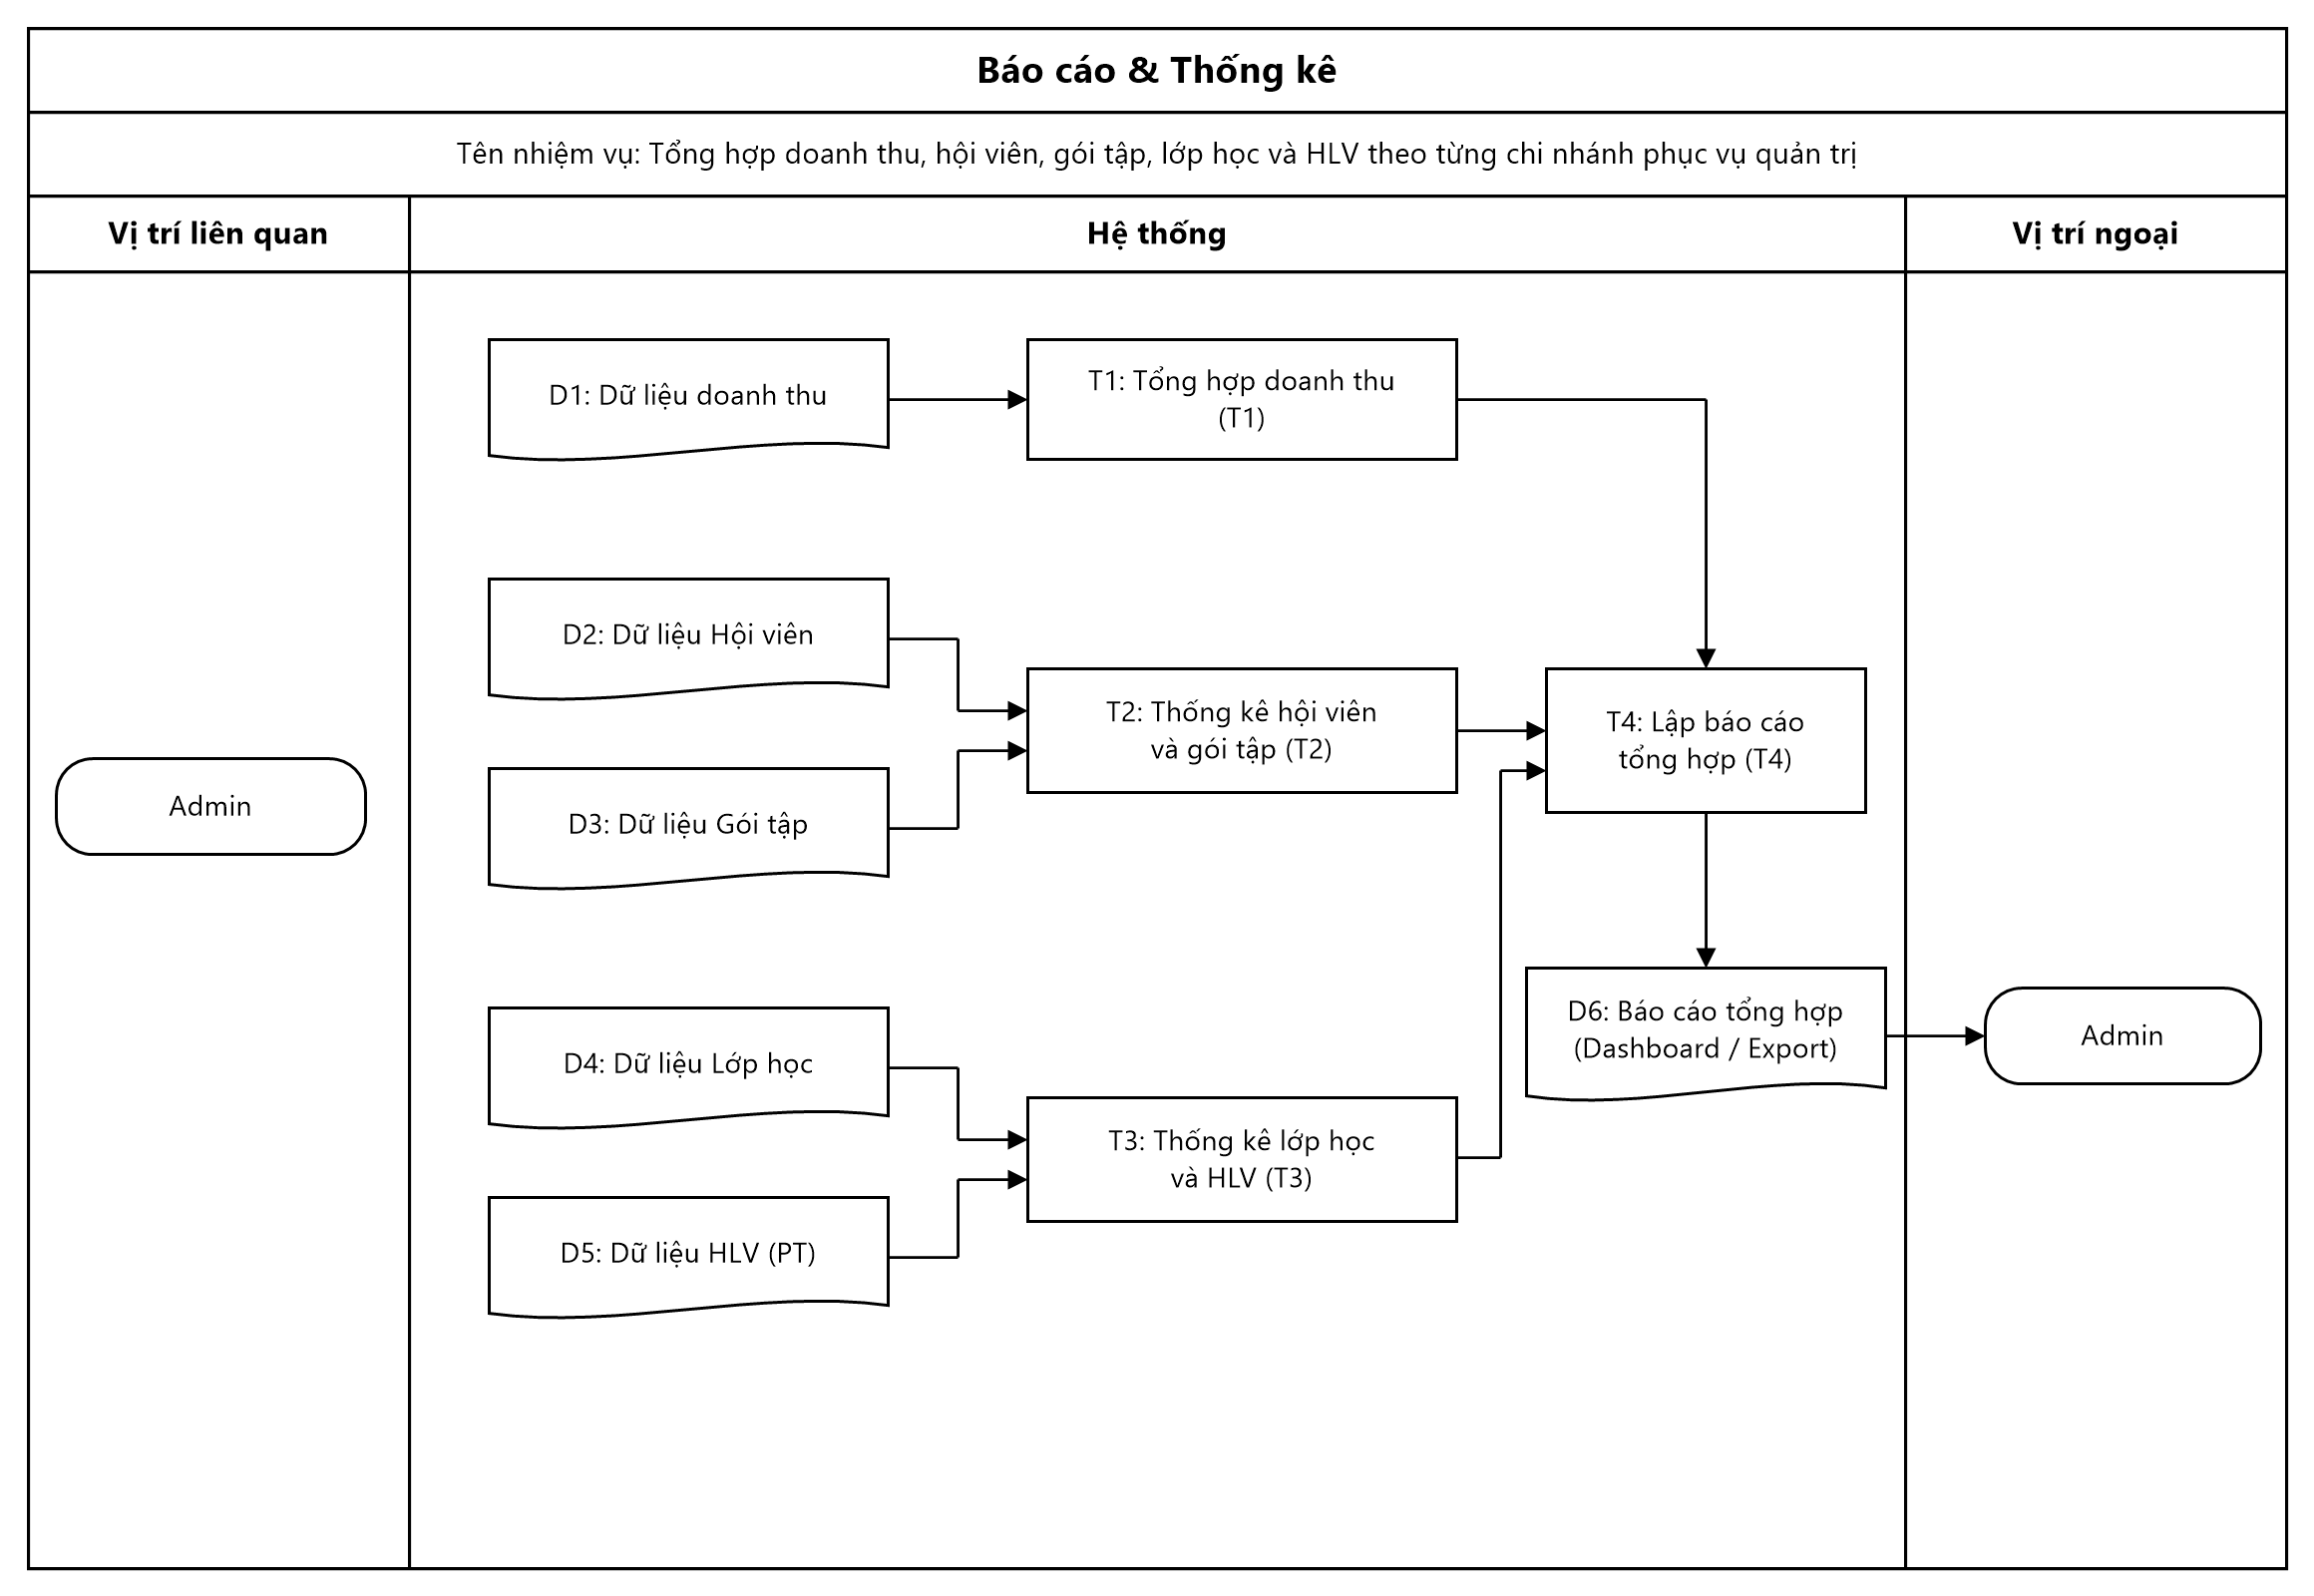
\includegraphics[width=0.88\textwidth, height=0.68\textheight, keepaspectratio]{images/ht_p55_1.png}
\caption{Sơ đồ hiện trạng 10: Báo cáo \& Thống kê}
\end{figure}

\begin{longtable}{|c|L{1.3cm}|p{10.8cm}|L{1.8cm}|}
\hline \textbf{STT} & \textbf{Hồ sơ} & \textbf{Vai trò} & \textbf{Công việc} \\ \hline \endfirsthead
\hline \textbf{STT} & \textbf{Hồ sơ} & \textbf{Vai trò} & \textbf{Công việc} \\ \hline \endhead \hline \endfoot
\hline
\caption{Mô tả hồ sơ -- Báo cáo \& Thống kê} \\
\endlastfoot
1 & D1 & Dữ liệu doanh thu: ghi nhận doanh thu từ đăng ký/gia hạn gói tập, dịch vụ theo chi nhánh. & T1, T4 \\ \hline
2 & D2 & Danh sách hội viên: số lượng hội viên, hội viên mới, ngừng hoạt động và biến động theo chi nhánh. & T2, T4 \\ \hline
3 & D3 & Dữ liệu gói tập: số lượng hội viên đang sử dụng, hết hạn và tình trạng sử dụng gói tập. & T2, T4 \\ \hline
4 & D4 & Dữ liệu lớp học: thông tin lớp, số lượng đăng ký, tham gia và sức chứa của từng lớp. & T3, T4 \\ \hline
5 & D5 & Dữ liệu huấn luyện viên: số buổi huấn luyện, số hội viên phục vụ và điểm đánh giá HLV. & T3, T4 \\* \hline
6 & D6 & Báo cáo tổng hợp: tập hợp các chỉ số doanh thu, hội viên, gói tập, lớp học và HLV theo chi nhánh. & T4 \\ \hline
\end{longtable}

{\setlength{\tabcolsep}{4pt}
\begin{longtable}{|L{0.9cm}|L{4.0cm}|L{2.5cm}|L{2.9cm}|L{1.7cm}|L{1.4cm}|L{1.4cm}|}
\hline \textbf{Mã} & \textbf{Mô tả công việc} & \textbf{Điều kiện khởi động} & \textbf{Quy tắc} & \textbf{Vị trí} & \textbf{Nhập} & \textbf{Xuất} \\ \hline \endfirsthead
\hline \textbf{Mã} & \textbf{Mô tả công việc} & \textbf{Điều kiện khởi động} & \textbf{Quy tắc} & \textbf{Vị trí} & \textbf{Nhập} & \textbf{Xuất} \\ \hline \endhead \hline \endfoot
\hline
\caption{Mô tả công việc -- Báo cáo \& Thống kê} \\
\endlastfoot
T1 & Tổng hợp doanh thu: Tổng hợp doanh thu gói hội viên, gói PT và dịch vụ khác theo chi nhánh/kỳ. & Khi Admin yêu cầu hoặc đến kỳ báo cáo. & Chỉ tổng hợp từ các giao dịch thanh toán thành công hợp lệ. & Admin / Hệ thống & D1 & Số liệu doanh thu \\ \hline
T2 & Thống kê hội viên và gói tập: Thống kê hội viên mới, hiện tại, ngừng hoạt động và tình trạng gói. & Khi Admin yêu cầu hoặc đến kỳ báo cáo. & Chỉ thống kê dữ liệu hội viên và gói tập hợp lệ trong hệ thống. & Admin / QL chi nhánh & D2, D3 & Số liệu HV \& gói \\ \hline
T3 & Thống kê lớp học và HLV: Tính tỷ lệ lấp đầy, tỷ lệ tham gia, số buổi dạy và đánh giá HLV. & Khi Admin yêu cầu báo cáo hiệu suất lớp hoặc HLV. & Chỉ tính các lớp và buổi huấn luyện đã ghi nhận trong hệ thống. & Admin / QL chi nhánh & D4, D5 & Số liệu lớp \& HLV \\ \hline
T4 & Lập báo cáo tổng hợp: Tổng hợp toàn bộ chỉ số theo từng chi nhánh và hiển thị dashboard. & Cuối ngày/tháng hoặc khi Admin yêu cầu. & Cho phép lọc theo chi nhánh và khoảng thời gian từ dữ liệu đã xác nhận. & Admin & D1--D5 & D6 \\ \hline
\end{longtable}
}

\subsubsection{Sơ đồ hiện trạng 11: Nghiệp vụ Thông báo}
\begin{figure}[H]
\centering
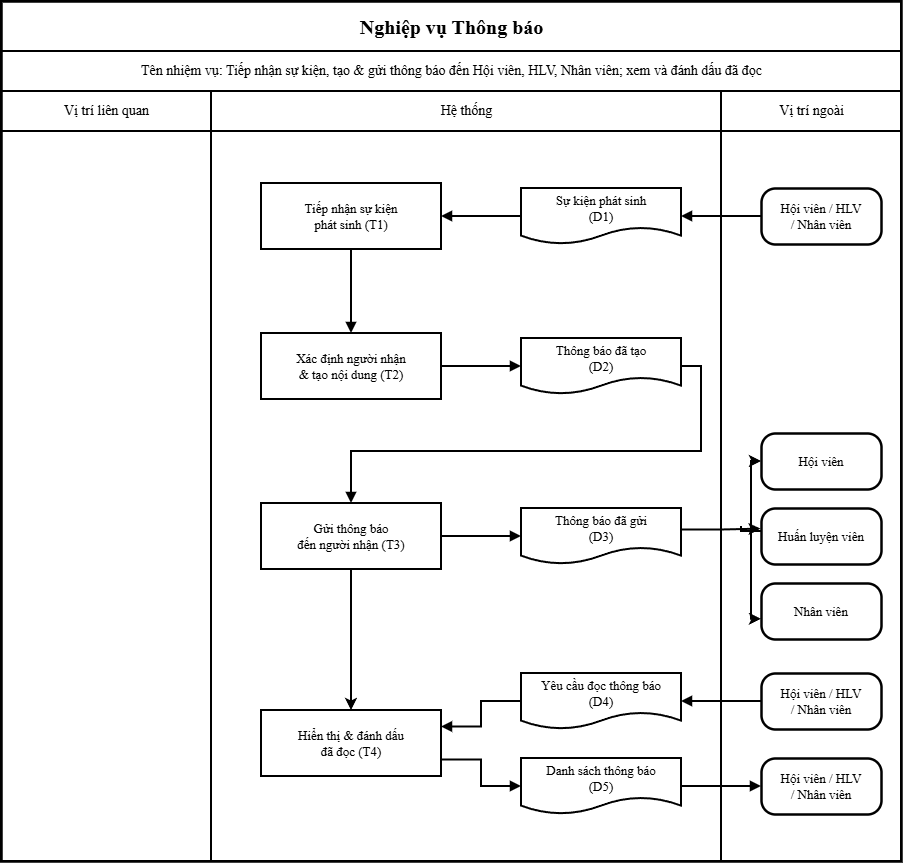
\includegraphics[width=0.90\textwidth, height=0.70\textheight, keepaspectratio]{images/ht_p60_1.png}
\caption{Sơ đồ hiện trạng 11: Nghiệp vụ Thông báo}
\end{figure}

\begin{longtable}{|c|L{1.3cm}|p{10.8cm}|L{1.8cm}|}
\hline \textbf{STT} & \textbf{Hồ sơ} & \textbf{Vai trò} & \textbf{Công việc} \\ \hline \endfirsthead
\hline \textbf{STT} & \textbf{Hồ sơ} & \textbf{Vai trò} & \textbf{Công việc} \\ \hline \endhead \hline \endfoot
\hline
\caption{Mô tả hồ sơ -- Nghiệp vụ Thông báo} \\
\endlastfoot
1 & D1 & Sự kiện phát sinh: thông tin về sự kiện cần tạo thông báo do Hội viên / HLV / Nhân viên cung cấp. & T1 \\ \hline
2 & D2 & Thông báo đã tạo: nội dung thông báo và thông tin người nhận xác định từ quy tắc thông báo. & T2, T3 \\ \hline
3 & D3 & Thông báo đã gửi: thông tin thông báo sau khi được gửi đến người nhận. & T3, T4 \\ \hline
4 & D4 & Yêu cầu đọc thông báo: yêu cầu xem thông báo của Hội viên / HLV / Nhân viên. & T4 \\* \hline
5 & D5 & Danh sách thông báo: danh sách các thông báo được hiển thị cho Hội viên / HLV / Nhân viên. & T4 \\ \hline
\end{longtable}

{\setlength{\tabcolsep}{4pt}
\begin{longtable}{|L{0.9cm}|L{4.0cm}|L{2.5cm}|L{2.9cm}|L{1.7cm}|L{1.4cm}|L{1.4cm}|}
\hline \textbf{Mã} & \textbf{Mô tả công việc} & \textbf{Điều kiện khởi động} & \textbf{Quy tắc} & \textbf{Vị trí} & \textbf{Nhập} & \textbf{Xuất} \\ \hline \endfirsthead
\hline \textbf{Mã} & \textbf{Mô tả công việc} & \textbf{Điều kiện khởi động} & \textbf{Quy tắc} & \textbf{Vị trí} & \textbf{Nhập} & \textbf{Xuất} \\ \hline \endhead \hline \endfoot
\hline
\caption{Mô tả công việc -- Nghiệp vụ Thông báo} \\
\endlastfoot
T1 & Tiếp nhận sự kiện phát sinh: Tiếp nhận thông tin sự kiện từ Hội viên, HLV hoặc Nhân viên. & Có sự kiện phát sinh cần thông báo. & Sự kiện phải có đầy đủ thông tin cần thiết để tạo thông báo. & Hệ thống & D1 & D1 \\ \hline
T2 & Xác định người nhận \& tạo nội dung: Xác định đối tượng nhận và tạo nội dung phù hợp. & Có sự kiện phát sinh. & Thông báo phải gửi đúng đối tượng và có nội dung phù hợp. & Hệ thống & D1 & D2 \\ \hline
T3 & Gửi thông báo đến người nhận: Gửi thông báo đã tạo đến Hội viên, HLV hoặc Nhân viên. & Có thông báo đã được tạo. & Gửi đúng người nhận theo quy tắc thông báo. & Hệ thống & D2 & D3 \\ \hline
T4 & Hiển thị \& đánh dấu đã đọc: Hiển thị danh sách thông báo và cập nhật trạng thái khi người dùng đọc. & Người dùng yêu cầu xem thông báo. & Chỉ hiển thị thông báo thuộc người nhận và cập nhật đã đọc khi xem. & Hệ thống & D3, D4 & D5 \\ \hline
\end{longtable}
}

% ==============================================================================
% 2. MÔ HÌNH HÓA YÊU CẦU
% ==============================================================================
\newpage
\section{Mô hình hóa yêu cầu}

\subsection{Sơ đồ Use-case}

\subsubsection{Sơ đồ Use-case tổng quát}
Sơ đồ Use-case tổng quát (mức khái niệm) của hệ thống \textbf{DFGymCenter} khái quát hóa phạm vi chức năng thành 12 nhóm Use-case cốt lõi cùng sự tương tác với 5 tác nhân (Actors); các chức năng này được phân rã chi tiết thành 21 nhóm Use-case cụ thể trong Bảng danh sách Use-case và mục 2.1.4 bên dưới.

\begin{figure}[H]
\centering
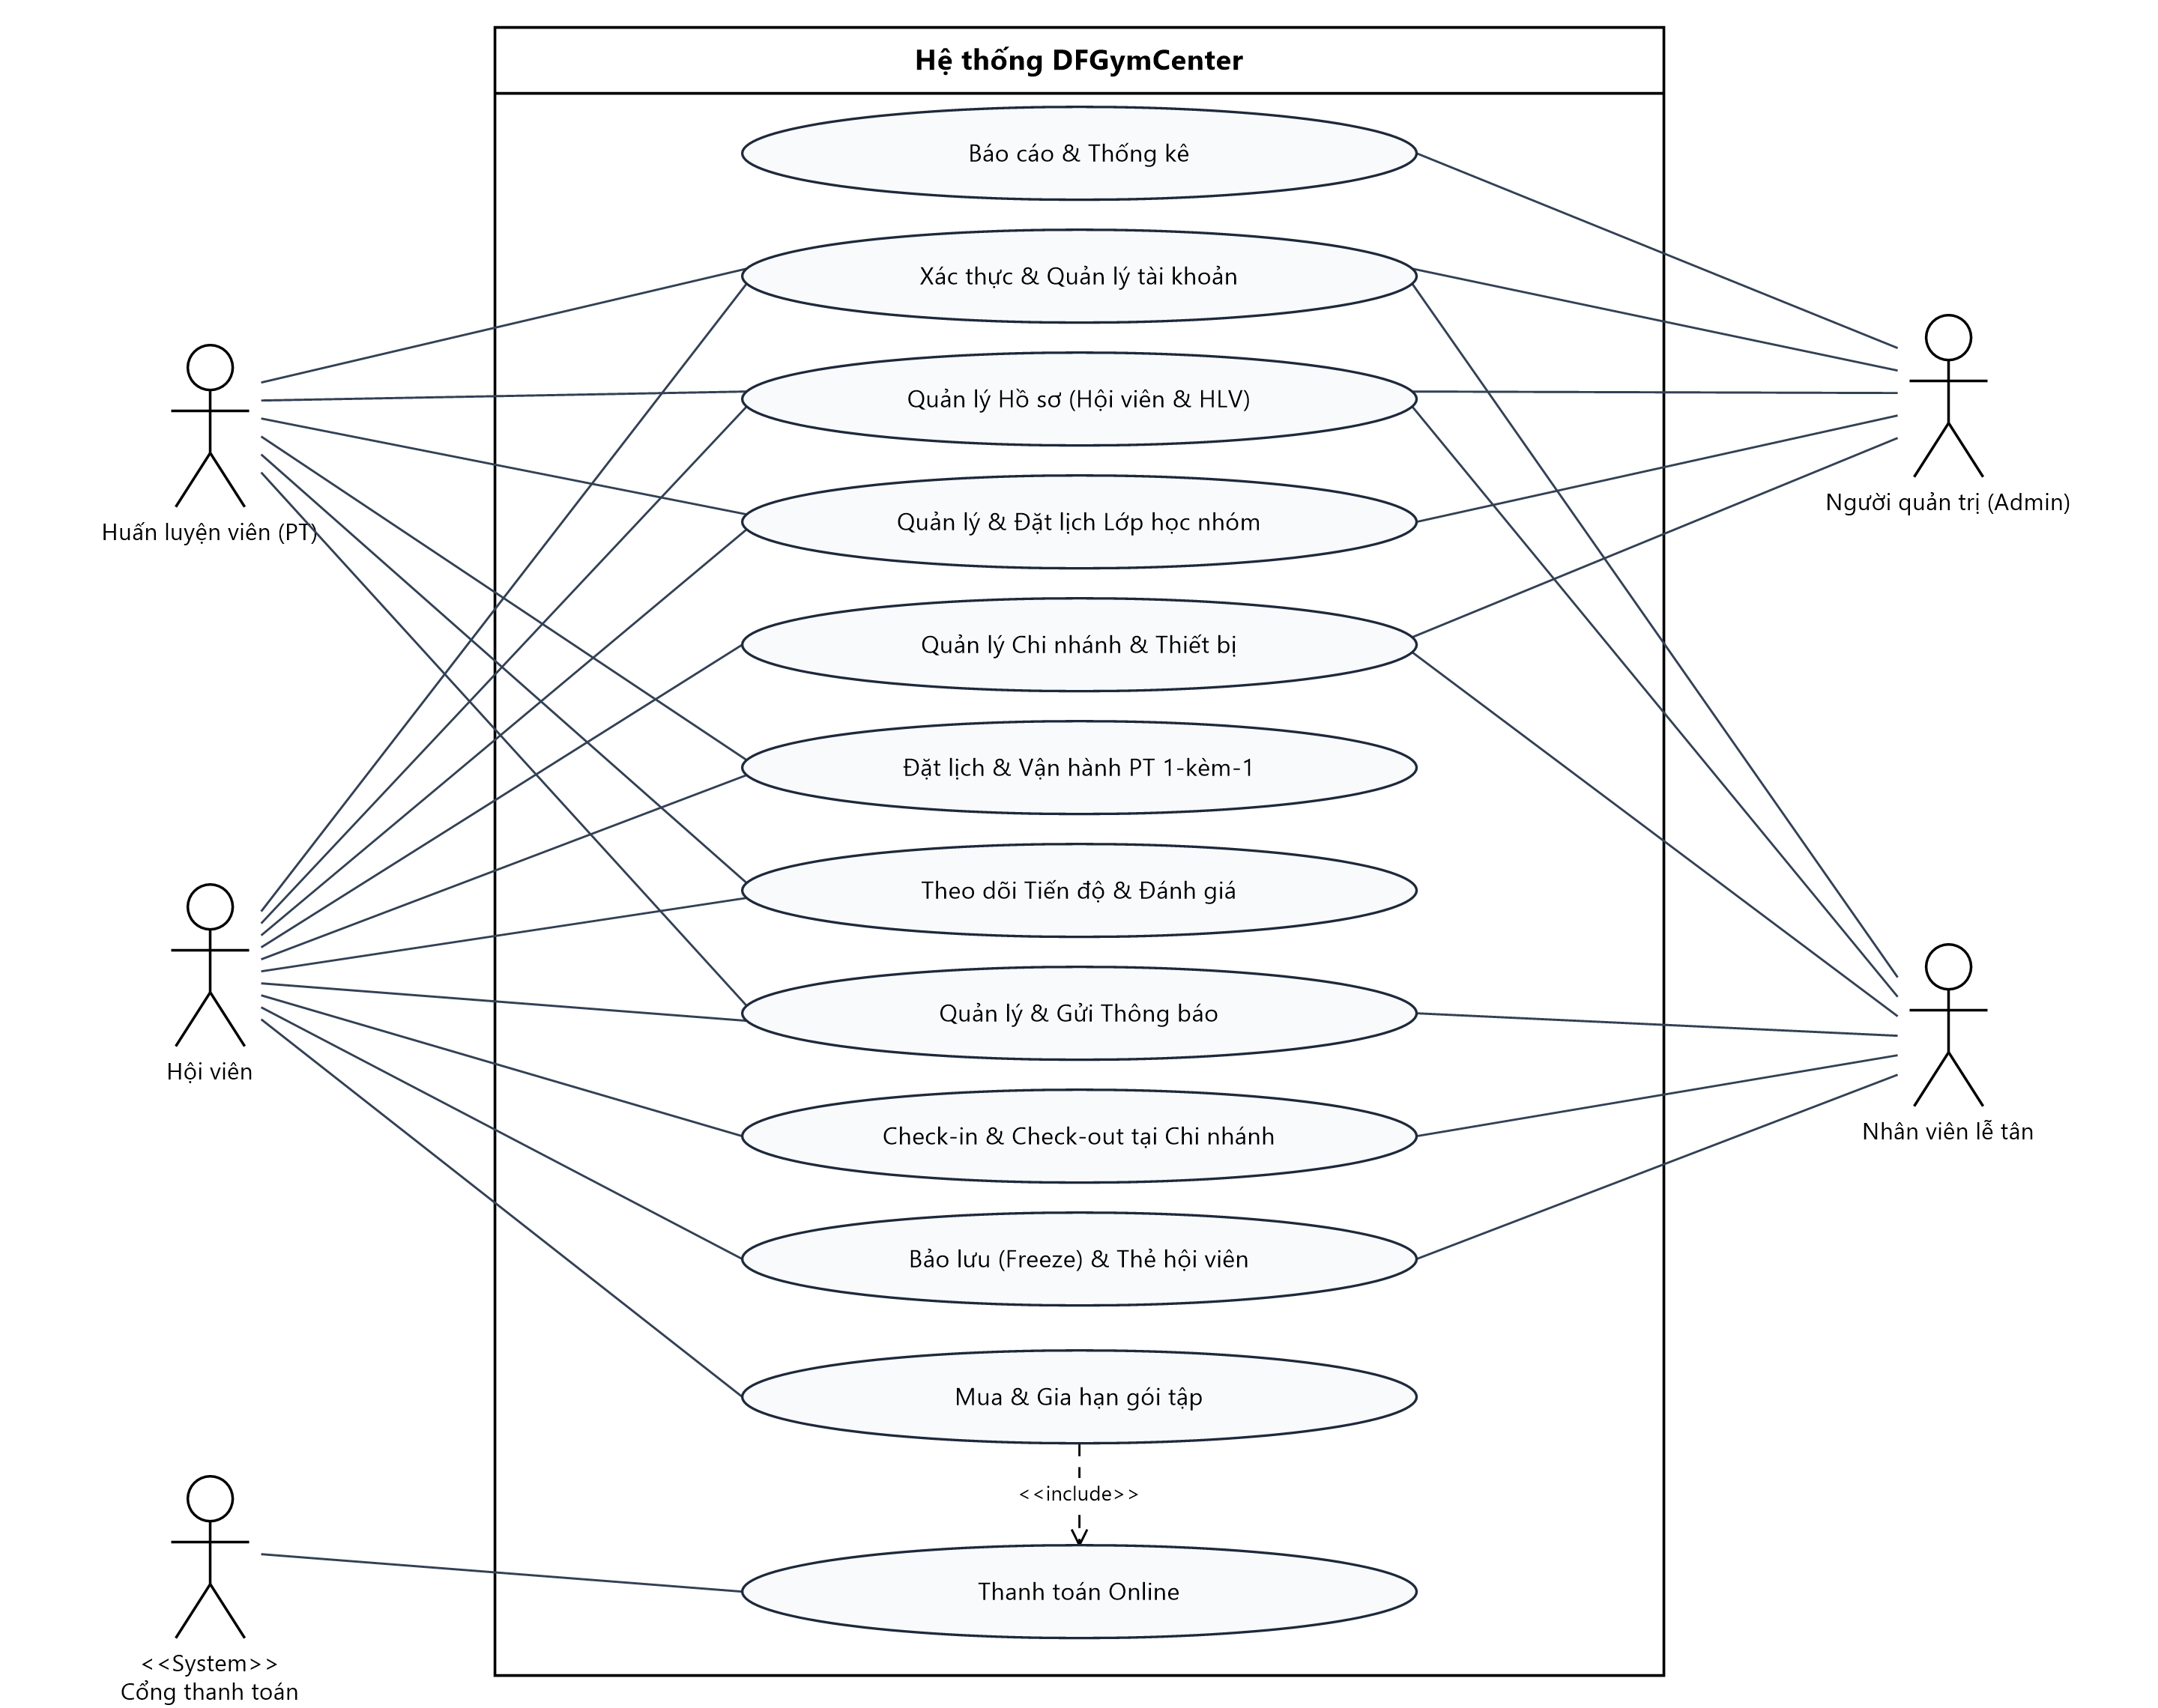
\includegraphics[width=0.88\textwidth, height=0.65\textheight, keepaspectratio]{images/uc_p03_1.png}
\caption{Sơ đồ Use-case tổng quát hệ thống DFGymCenter}
\end{figure}

\subsubsection{Danh sách các Actor}

\begin{table}[H]
\centering
\begin{tabularx}{\textwidth}{|c|L{3.8cm}|Y|}
\hline
\textbf{STT} & \textbf{Tên Actor} & \textbf{Ý nghĩa / Ghi chú} \\ \hline
1 & Hội viên (Member) & Là đối tượng sử dụng dịch vụ cuối cùng, thực hiện các thao tác như đăng ký tài khoản, mua/gia hạn gói tập, đặt lịch lớp/PT, check-in, cập nhật chỉ số cơ thể, phản ánh sự cố và đánh giá chất lượng sau buổi tập. \\ \hline
2 & Huấn luyện viên (PT) & Là nhân sự chuyên môn, thực hiện cập nhật và quản lý hồ sơ cá nhân, thiết lập lịch rảnh, nhận/duyệt/từ chối lịch hẹn 1-kèm-1, giảng dạy các lớp nhóm và điểm danh xác nhận hội viên tham gia. \\ \hline
3 & Nhân viên lễ tân (Staff) & Là người vận hành tại quầy, phụ trách xử lý yêu cầu đóng băng (freeze) gói tập, nhập check-in/check-out thủ công khi hội viên quên thẻ hoặc thiết bị lỗi, cấp/khóa thẻ thành viên và tiếp nhận/xử lý sự cố thiết bị. \\ \hline
4 & Người quản trị (Admin) & Là người có quyền hạn cao nhất, phụ trách quản lý tài khoản người dùng, phân quyền, danh mục gói tập, thông tin chi nhánh, danh sách thiết bị, khởi tạo và phân công lớp học, cũng như theo dõi báo cáo thống kê đa chiều. \\ \hline
5 & Cổng thanh toán (\texttt{<{}<System>{}>} Payment Gateway) & Là tác nhân hệ thống bên ngoài (VNPay / ZaloPay), tiếp nhận yêu cầu thanh toán trực tuyến khi hội viên mua mới hoặc gia hạn gói tập, xử lý giao dịch và gửi phản hồi (callback) kết quả thành công/thất bại về hệ thống DFGymCenter. \\ \hline
\end{tabularx}
\caption{Danh sách các Actor trong hệ thống DFGymCenter}
\end{table}

\subsubsection{Danh sách các Use-case}
Bảng dưới đây ánh xạ đầy đủ 12 nhóm Use-case khái niệm ở sơ đồ tổng quát (mục 2.1.1) sang 21 phân nhóm Use-case chi tiết (được phân rã và đặc tả tại mục 2.1.4):

{\small
\setlength{\tabcolsep}{4pt}
\renewcommand{\arraystretch}{1.08}
\begin{longtable}{|c|L{3.5cm}|L{3.9cm}|L{7.3cm}|}
\hline
\textbf{STT} & \textbf{Nhóm tổng quát} & \textbf{Use-case phân rã} & \textbf{Ý nghĩa / Mô tả ngắn} \\ \hline
\endfirsthead
\hline
\textbf{STT} & \textbf{Nhóm tổng quát} & \textbf{Use-case phân rã} & \textbf{Ý nghĩa / Mô tả ngắn} \\ \hline
\endhead
\hline
\endfoot
\hline
\caption{Danh sách tổng hợp các Use-case của hệ thống DFGymCenter} \\
\endlastfoot
1 & Xác thực \& Quản lý tài khoản & Đăng ký tài khoản & Cho phép Hội viên hoặc Huấn luyện viên tạo tài khoản mới trên hệ thống bằng cách điền thông tin cá nhân (họ tên, email, SĐT, giới tính, ngày sinh, mật khẩu) mà không cần bước xác minh OTP. \\ \hline
2 & Xác thực \& Quản lý tài khoản & Đăng nhập / Đăng xuất & Chức năng xác thực để người dùng truy cập vào tài khoản cá nhân theo vai trò và thoát khỏi hệ thống an toàn. \\ \hline
3 & Xác thực \& Quản lý tài khoản & Đổi mật khẩu / Quên mật khẩu & Giúp người dùng quản lý thông tin bảo mật và khôi phục quyền truy cập tài khoản qua OTP/Reset Link khi cần. \\ \hline
4 & Quản lý Hồ sơ (Hội viên \& HLV) & Quản lý hồ sơ hội viên \& Ghi nhận chỉ số cơ thể ban đầu & Hội viên tra cứu, cập nhật thông tin cá nhân mở rộng và tự ghi nhận mốc chỉ số cơ thể đầu tiên (chiều cao, cân nặng, BMI...) làm chuẩn theo dõi tiến độ; Lễ tân và Admin tra cứu thông tin hồ sơ hội viên. \\ \hline
5 & Quản lý Hồ sơ (Hội viên \& HLV) & Quản lý hồ sơ huấn luyện viên & Huấn luyện viên khai báo và cập nhật thông tin chuyên môn, bằng cấp, kinh nghiệm làm việc và chi nhánh phụ trách để Admin phê duyệt. \\ \hline
6 & Xác thực \& Quản lý tài khoản & Tạo \& Gán chi nhánh cho Lễ tân & Admin tạo tài khoản cho nhân viên lễ tân và phân công làm việc tại một chi nhánh cụ thể. \\ \hline
7 & Xác thực \& Quản lý tài khoản & Quản lý phân quyền \& Khóa/Mở khóa tài khoản & Admin xem danh sách tất cả tài khoản, thay đổi quyền hạn hoặc thực hiện khóa/mở khóa tài khoản người dùng khi cần thiết. \\ \hline
8 & Mua \& Gia hạn gói tập & Mua gói tập & Hội viên lựa chọn gói hội viên (tháng, quý, năm) hoặc gói PT 1-kèm-1 và thực hiện thanh toán qua Cổng thanh toán để sử dụng dịch vụ. \\ \hline
9 & Mua \& Gia hạn gói tập & Gia hạn gói tập & Hội viên gia hạn gói tập đang dùng hoặc sắp hết hạn qua Cổng thanh toán, thời gian sử dụng mới được cộng nối tiếp. \\ \hline
10 & Thanh toán Online & Thanh toán Online & Hệ thống kết nối với Cổng thanh toán để xử lý, ghi nhận kết quả giao dịch thành công/thất bại và kích hoạt gói tập cho hội viên. \\ \hline
11 & Quản lý \& Đặt lịch Lớp học nhóm & Quản lý \& Đặt lịch Lớp học nhóm & Admin tạo lớp và phân công HLV. Hội viên đặt chỗ tham gia lớp; hệ thống kiểm tra gói tập và xếp chỗ hoặc đưa vào danh sách chờ (Waitlist) nếu lớp đầy. \\ \hline
12 & Đặt lịch \& Vận hành PT 1-kèm-1 & Đặt và Hủy lịch lớp PT & Hội viên xem lịch rảnh của HLV để gửi yêu cầu đặt lịch 1-kèm-1, hoặc hủy các buổi tập đã đặt theo quy định thời hạn. \\ \hline
13 & Đặt lịch \& Vận hành PT 1-kèm-1 & Xác nhận yêu cầu và cập nhật lịch rảnh & PT chủ động thiết lập khung giờ rảnh cá nhân (đối chiếu lịch lớp nhóm), đồng thời chấp nhận hoặc từ chối yêu cầu đặt lịch từ hội viên. \\ \hline
14 & Check-in \& Check-out tại Chi nhánh & Check-in \& Check-out tại Chi nhánh & Hội viên dùng thẻ/QR để hệ thống tự động kiểm tra hiệu lực gói tập và quyền chi nhánh trước khi vào/ra. Lễ tân nhập thủ công khi cần; hệ thống tự động check-out lúc đóng cửa. \\ \hline
15 & Quản lý Chi nhánh \& Thiết bị & Chi nhánh \& Thiết bị & Admin thêm mới, cấu hình chi nhánh, gói áp dụng và danh mục thiết bị. Hội viên phản ánh sự cố; Lễ tân tiếp nhận và cập nhật trạng thái xử lý. \\ \hline
16 & Theo dõi Tiến độ \& Đánh giá & Theo dõi Tiến độ \& Đánh giá & Hội viên nhập chỉ số cơ thể để xem biểu đồ tiến độ so với mốc ban đầu; đồng thời đánh giá chấm điểm cho PT/Lớp học sau khi được xác nhận tham gia. \\ \hline
17 & Báo cáo \& Thống kê & Báo cáo \& Thống kê & Hệ thống tổng hợp doanh thu, hội viên (churn rate), tình trạng gói tập, hiệu suất lớp học và đánh giá PT để Admin theo dõi, xuất báo cáo (Excel/PDF). \\ \hline
18 & Quản lý \& Gửi Thông báo & Xem danh sách thông báo & Hội viên, Huấn luyện viên hoặc Lễ tân xem lại lịch sử thông báo đã nhận, xem chi tiết và đánh dấu đã đọc. \\ \hline
19 & Quản lý \& Gửi Thông báo & Gửi thông báo tự động & Hệ thống tự động tạo và phát thông báo (nhắc lịch tập, đổi lịch, gói sắp hết hạn, kết quả duyệt lịch PT, freeze, sự cố thiết bị...) khi có sự kiện phát sinh. \\ \hline
20 & Bảo lưu (Freeze) \& Thẻ hội viên & Bảo lưu / Tạm ngưng gói tập (Freeze) & Hội viên gửi yêu cầu tạm ngưng gói hội viên còn hiệu lực trong định mức cho phép; Nhân viên lễ tân thẩm định (duyệt/từ chối), tự động cộng bù ngày hết hạn và hủy lịch trùng. \\* \hline
21 & Bảo lưu (Freeze) \& Thẻ hội viên & Quản lý Thẻ hội viên (MemberCard) & Hội viên xem mã thẻ/QR cá nhân và báo mất thẻ (\texttt{Lost}); Nhân viên lễ tân tra cứu lịch sử thẻ, khóa/mở khóa hoặc cấp lại thẻ mới theo chính sách 01 thẻ \texttt{Active}. \\ \hline
\end{longtable}
}

\subsubsection{Đặc tả chi tiết các Use-case}
Dưới đây là sơ đồ Use-case phân rã và đặc tả chi tiết cho 21 nhóm chức năng nghiệp vụ của hệ thống DFGymCenter:

\paragraph{1. Đăng ký tài khoản}
\begin{figure}[H]
\centering
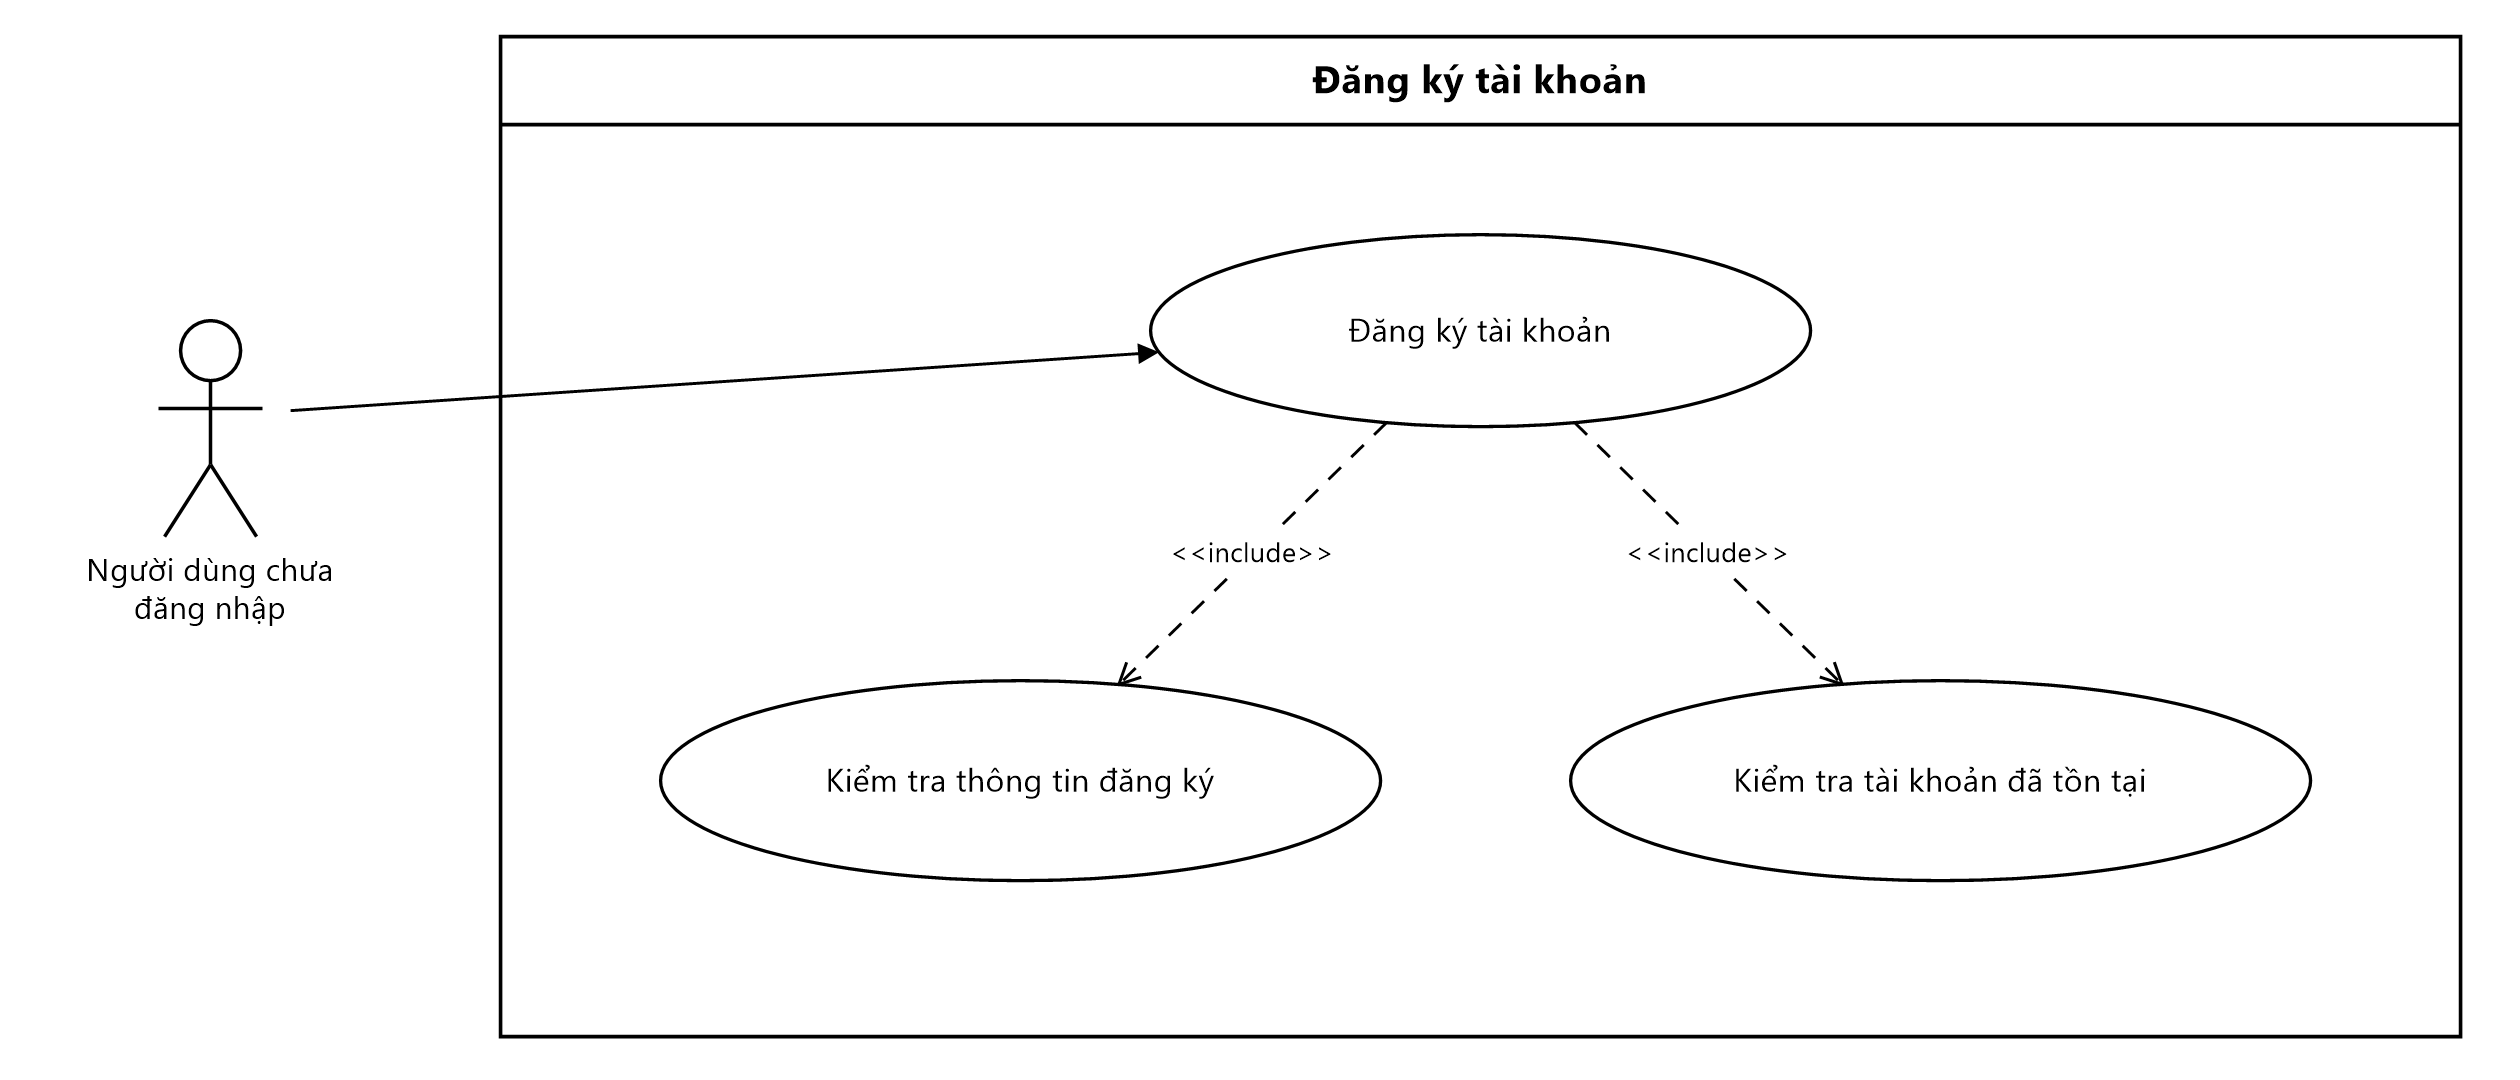
\includegraphics[width=0.88\textwidth, height=0.65\textheight, keepaspectratio]{images/uc_p05_1.png}
\caption{Use-case Đăng ký tài khoản}
\end{figure}
\begin{table}[H]\centering\footnotesize
\begin{tabularx}{\textwidth}{|L{3.2cm}|Y|}
\hline \textbf{Tóm tắt} & Cho phép người dùng chưa đăng nhập (Hội viên hoặc Huấn luyện viên) điền thông tin cá nhân để tạo tài khoản mới trên hệ thống mà không qua bước xác minh OTP qua email/SĐT. \\ \hline
\textbf{Tiền điều kiện} & Người dùng chưa đăng nhập và truy cập vào màn hình đăng ký của ứng dụng/website. \\ \hline
\textbf{Dòng sự kiện chính} & 1. Người dùng chọn vai trò cần đăng ký (Hội viên hoặc Huấn luyện viên; nếu là Huấn luyện viên thì chọn thêm chi nhánh làm việc, chuyên môn và số năm kinh nghiệm).\newline 2. Người dùng nhập thông tin đăng ký: Họ tên, Email, Số điện thoại, Giới tính, Ngày sinh, Mật khẩu và Xác nhận mật khẩu.\newline 3. Hệ thống thực hiện kiểm tra thông tin đăng ký (định dạng email/SĐT, mật khẩu tối thiểu 6 ký tự, khớp mật khẩu xác nhận) và kiểm tra tài khoản đã tồn tại hay chưa (email duy nhất).\newline 4. Hệ thống tạo và lưu tài khoản mới vào cơ sở dữ liệu (tự động cấp mã thẻ hội viên mặc định đối với Hội viên).\newline 5. Hệ thống hiển thị thông báo đăng ký thành công, tự động đăng nhập và chuyển người dùng sang trang hồ sơ cá nhân. \\ \hline
\textbf{Dòng sự kiện phụ} & Nếu Email đã tồn tại trong hệ thống, mật khẩu dưới 6 ký tự, mật khẩu xác nhận không khớp hoặc Huấn luyện viên chưa chọn chi nhánh, hệ thống hiển thị thông báo lỗi tương ứng và yêu cầu chỉnh sửa. \\ \hline
\textbf{Hậu điều kiện} & Tài khoản mới được tạo thành công trên hệ thống và người dùng được cấp phiên đăng nhập ngay. \\ \hline
\end{tabularx}
\caption{Bảng đặc tả Use-case 1: Đăng ký tài khoản}
\end{table}

\paragraph{2. Đăng nhập / Đăng xuất}
\begin{figure}[H]
\centering
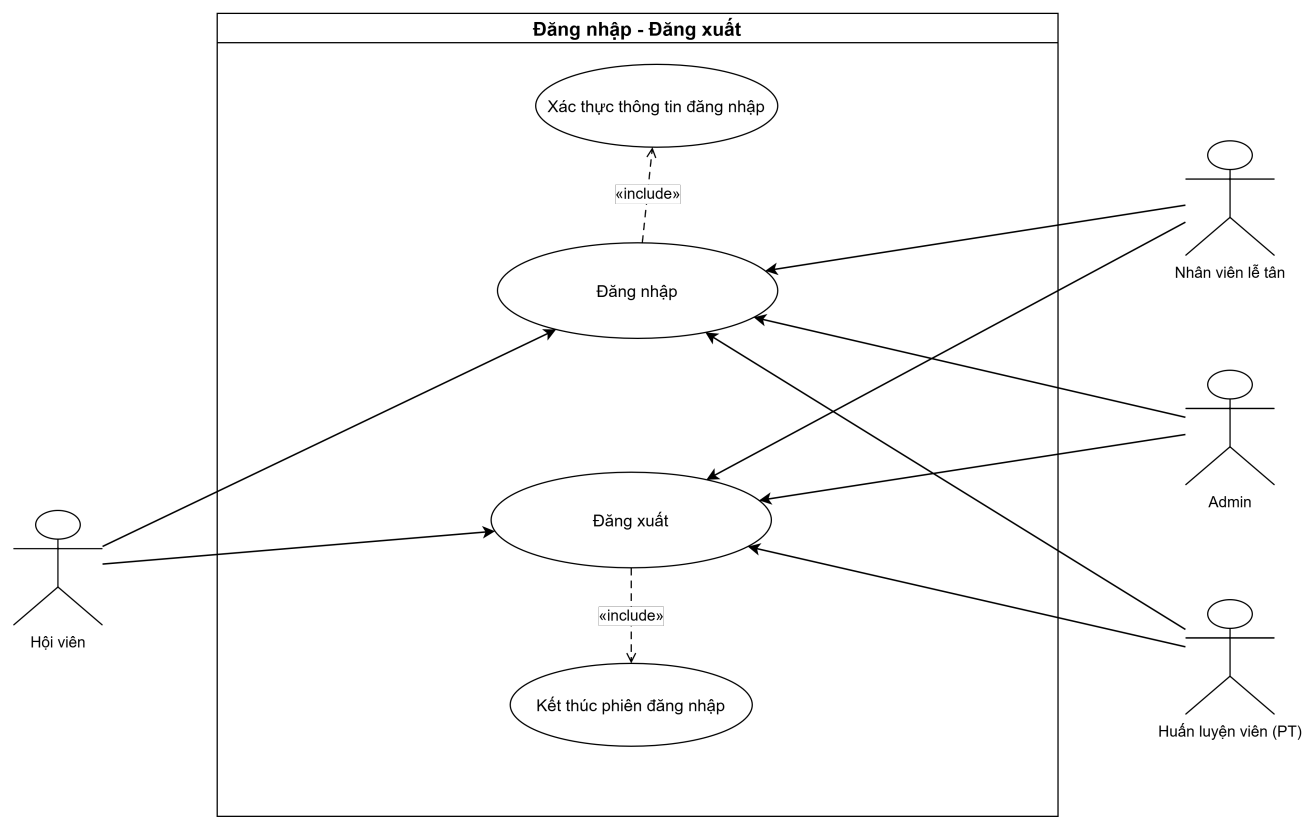
\includegraphics[width=0.88\textwidth, height=0.65\textheight, keepaspectratio]{images/uc_p07_1.png}
\caption{Use-case Đăng nhập / Đăng xuất}
\end{figure}
\begin{table}[H]\centering\footnotesize
\begin{tabularx}{\textwidth}{|L{3.2cm}|Y|}
\hline \textbf{Tóm tắt} & Xác thực thông tin tài khoản để cấp quyền truy cập hệ thống theo đúng vai trò hoặc kết thúc phiên làm việc. \\ \hline
\textbf{Tiền điều kiện} & Đối với đăng nhập: Tài khoản đã được tạo và không ở trạng thái bị khóa. Đối với đăng xuất: Người dùng đang trong phiên đăng nhập. \\ \hline
\textbf{Dòng sự kiện chính} & 1. Đăng nhập: Người dùng nhập Email/SĐT và Mật khẩu; hệ thống đối chiếu thông tin xác thực.\newline 2. Hệ thống kiểm tra vai trò (Role) và cấp phiên làm việc (Session/Token) tương ứng với vai trò (Member, PT, Lễ tân, Admin).\newline 3. Đăng xuất: Người dùng chọn Đăng xuất, hệ thống hủy phiên làm việc và quay lại màn hình đăng nhập. \\ \hline
\textbf{Dòng sự kiện phụ} & -- Nếu nhập sai thông tin xác thực quá số lần quy định, hệ thống cảnh báo hoặc tạm thời khóa đăng nhập.\newline -- Nếu tài khoản đang ở trạng thái bị khóa, hệ thống hiển thị thông báo "Tài khoản của bạn đã bị khóa". \\ \hline
\textbf{Hậu điều kiện} & Người dùng truy cập thành công vào đúng giao diện chức năng được phân quyền hoặc kết thúc phiên làm việc an toàn. \\ \hline
\end{tabularx}
\caption{Bảng đặc tả Use-case 2: Đăng nhập / Đăng xuất}
\end{table}

\paragraph{3. Đổi mật khẩu / Quên mật khẩu}
\begin{figure}[H]
\centering
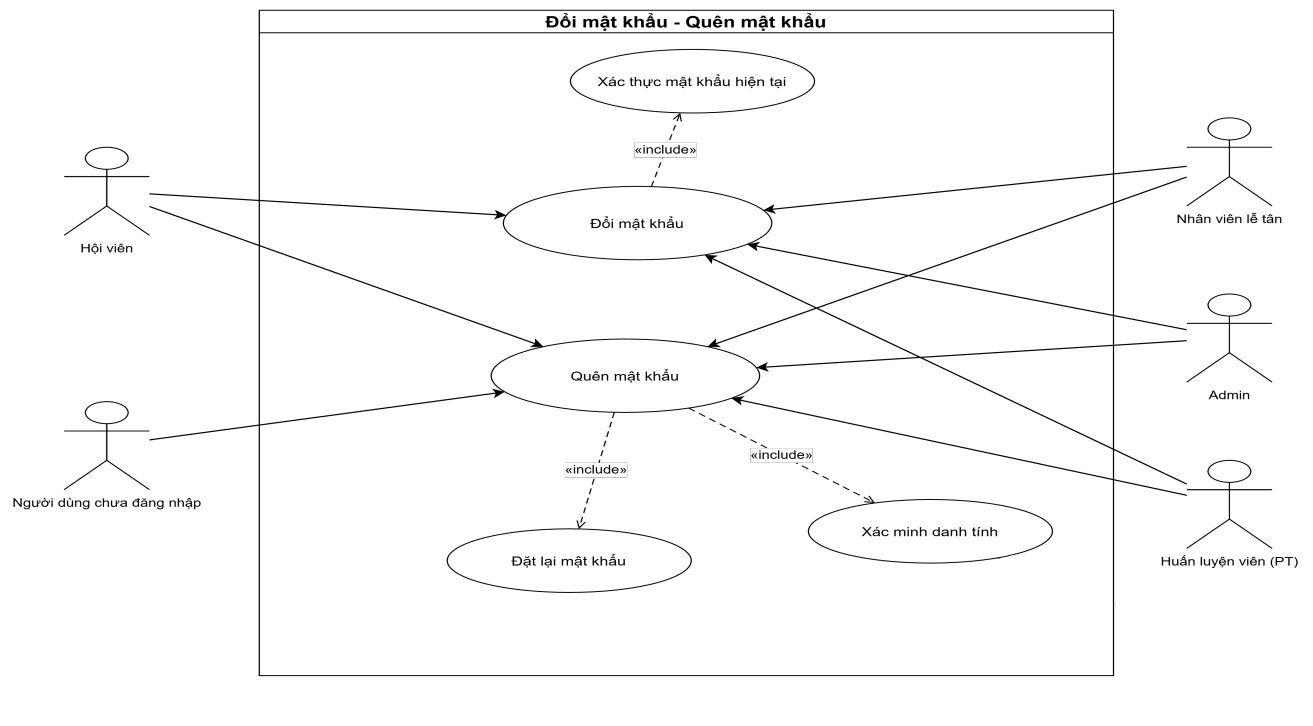
\includegraphics[width=0.88\textwidth, height=0.65\textheight, keepaspectratio]{images/uc_p08_1.png}
\caption{Use-case Đổi mật khẩu / Quên mật khẩu}
\end{figure}
\begin{table}[H]\centering\footnotesize
\begin{tabularx}{\textwidth}{|L{3.2cm}|Y|}
\hline \textbf{Tóm tắt} & Cho phép người dùng chủ động đổi mật khẩu mới hoặc thực hiện quy trình khôi phục mật khẩu qua Email/SĐT khi quên. \\ \hline
\textbf{Tiền điều kiện} & Có nhu cầu thay đổi/khôi phục mật khẩu. \\ \hline
\textbf{Dòng sự kiện chính} & -- Đổi mật khẩu: Người dùng nhập Mật khẩu hiện tại và Mật khẩu mới $\rightarrow$ Hệ thống xác nhận và cập nhật mật khẩu mới.\newline -- Quên mật khẩu: (1) Nhập Email/SĐT đã đăng ký; (2) Hệ thống tạo và gửi mã xác thực (OTP/Reset Link); (3) Người dùng nhập OTP / truy cập liên kết và thiết lập mật khẩu mới; (4) Hệ thống ghi nhận mật khẩu mới. \\ \hline
\textbf{Dòng sự kiện phụ} & Nếu mã OTP hết hạn hoặc không chính xác, hệ thống báo lỗi và cho phép yêu cầu gửi lại mã. \\ \hline
\textbf{Hậu điều kiện} & Mật khẩu tài khoản được cập nhật mới trên hệ thống. \\ \hline
\end{tabularx}
\caption{Bảng đặc tả Use-case 3: Đổi mật khẩu / Quên mật khẩu}
\end{table}

\paragraph{4. Quản lý hồ sơ hội viên \& Ghi nhận chỉ số cơ thể ban đầu}
\begin{figure}[H]
\centering
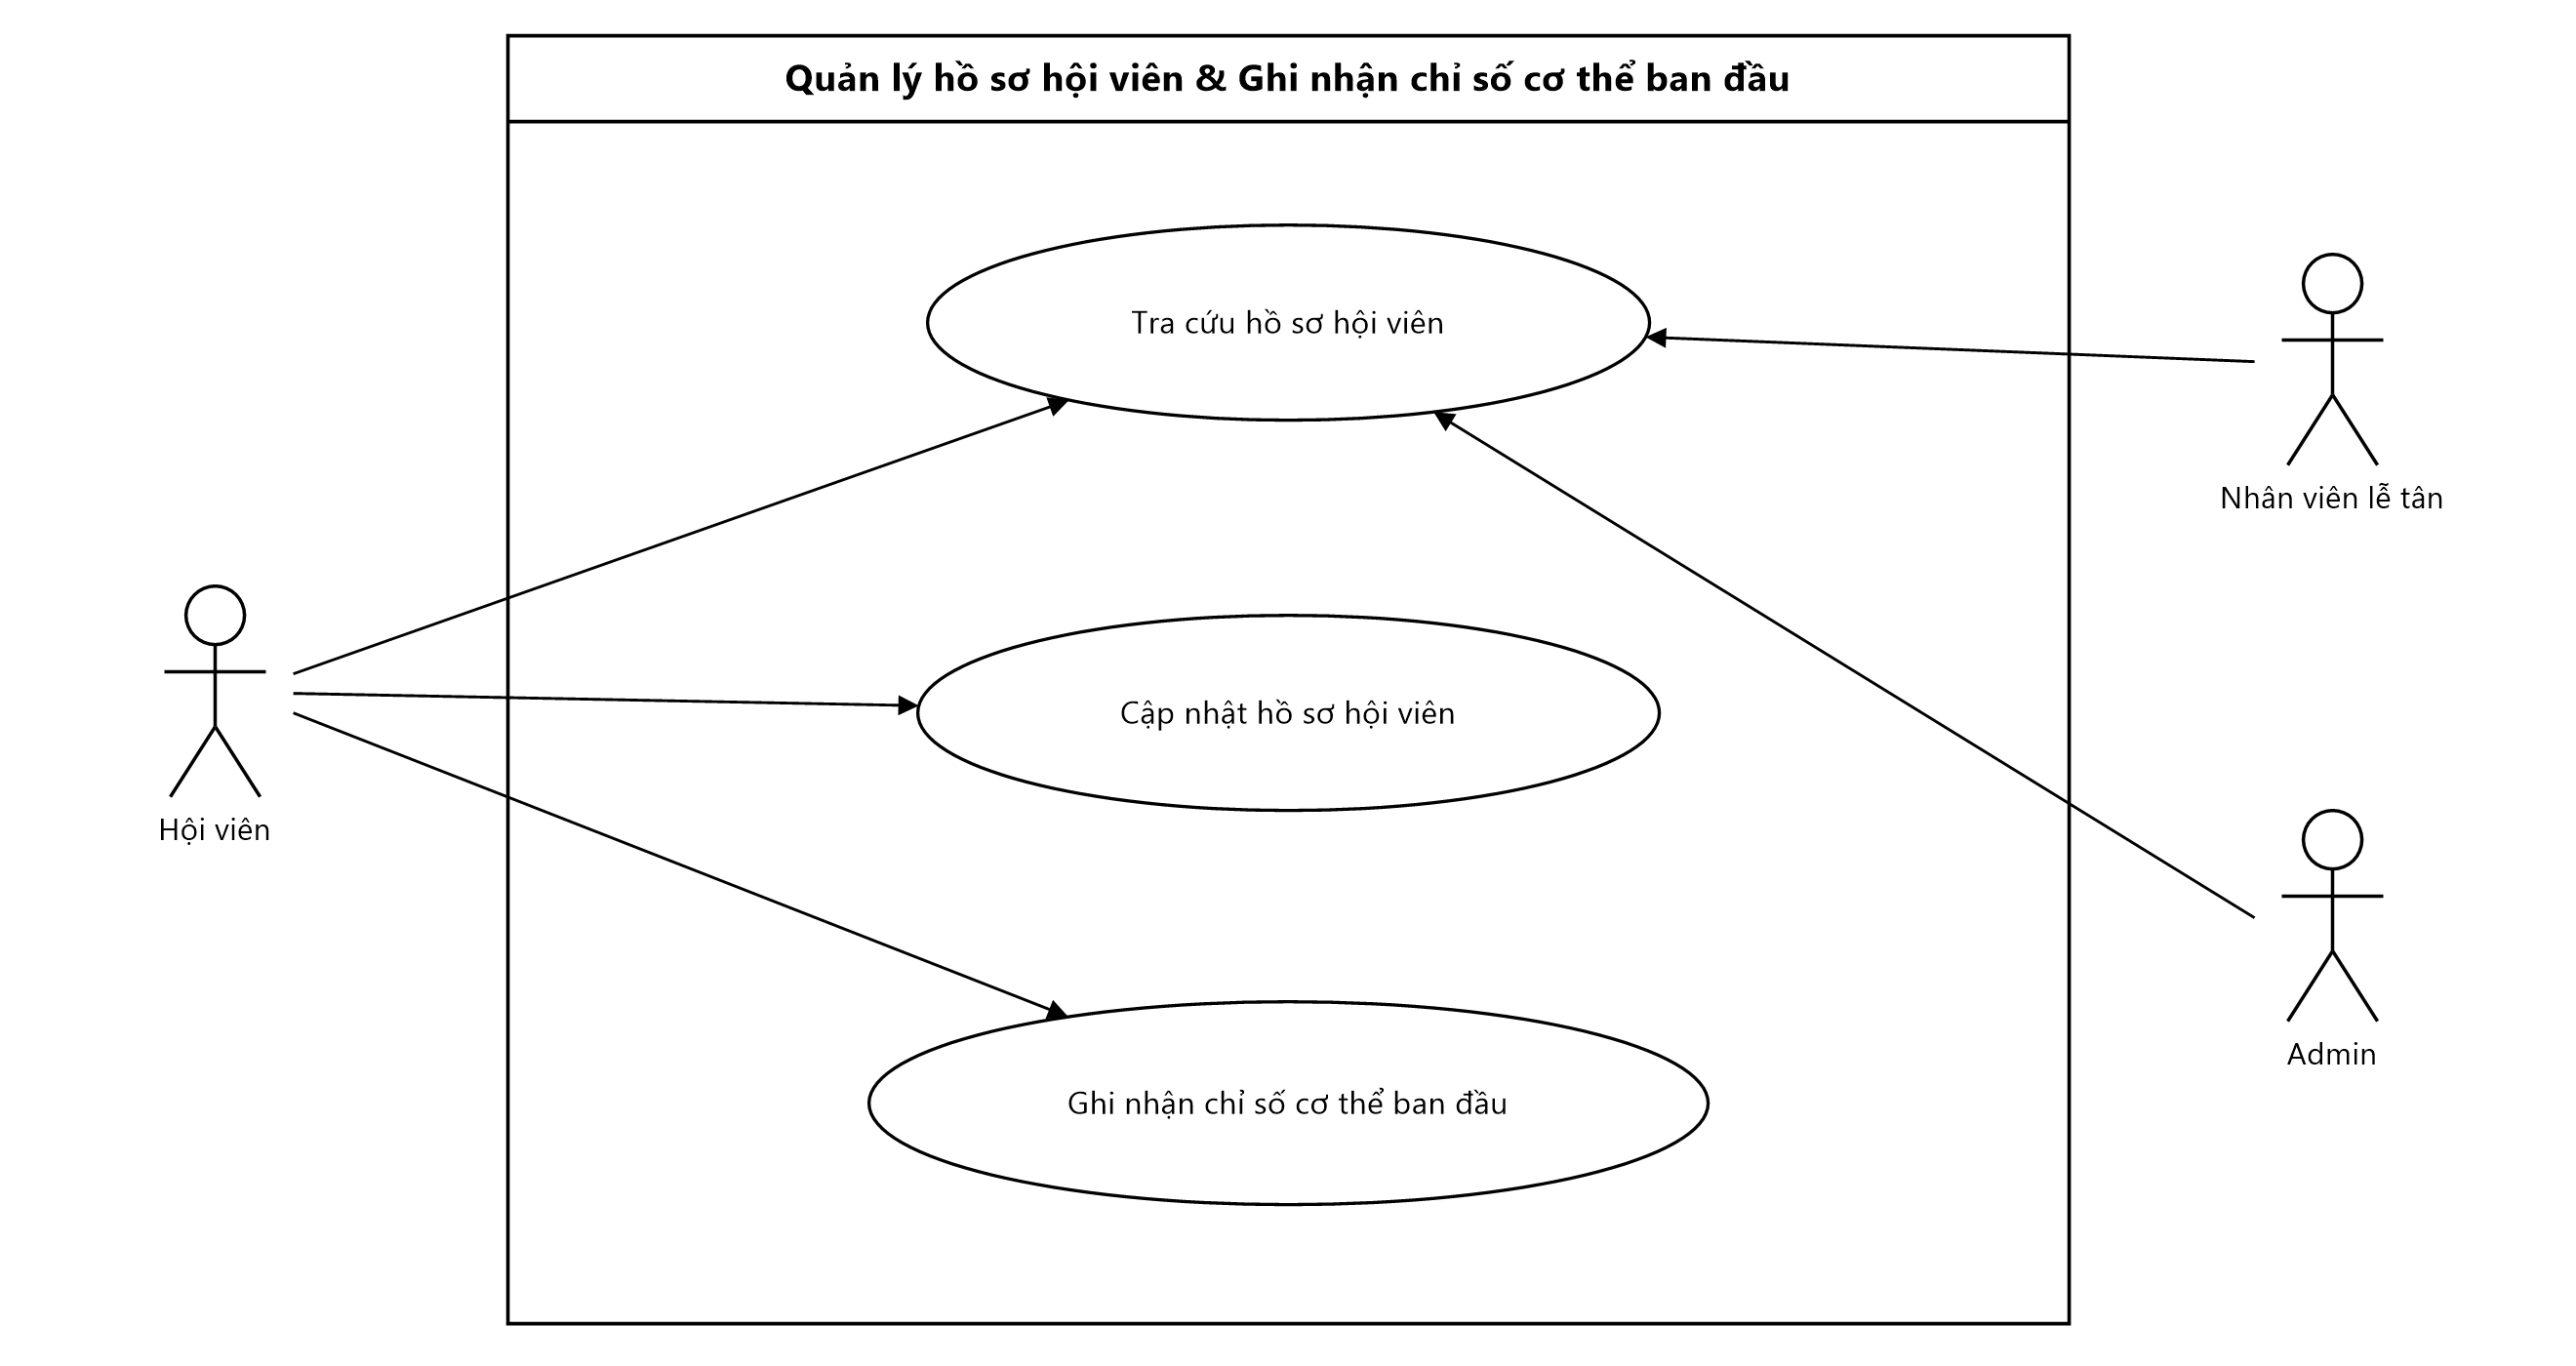
\includegraphics[width=0.88\textwidth, height=0.65\textheight, keepaspectratio]{images/uc_p09_1.png}
\caption{Use-case Quản lý hồ sơ hội viên \& Ghi nhận chỉ số cơ thể ban đầu}
\end{figure}
\begin{table}[H]\centering\footnotesize
\begin{tabularx}{\textwidth}{|L{3.2cm}|Y|}
\hline \textbf{Tóm tắt} & Cho phép Hội viên tra cứu, cập nhật thông tin cá nhân chi tiết và tự ghi nhận các chỉ số đo cơ thể đầu tiên (mốc Baseline) để làm chuẩn theo dõi tiến độ tập luyện; Nhân viên lễ tân và Admin tra cứu hồ sơ hội viên khi cần hỗ trợ. \\ \hline
\textbf{Tiền điều kiện} & Người dùng (Hội viên, Nhân viên lễ tân hoặc Admin) đã đăng nhập thành công vào hệ thống; hồ sơ hội viên đã được khởi tạo tự động khi đăng ký tài khoản. \\ \hline
\textbf{Dòng sự kiện chính} & 1. Hội viên truy cập trang Hồ sơ cá nhân (\texttt{/member/profile}) để xem hoặc cập nhật thông tin mở rộng (Họ tên, SĐT, ngày sinh, giới tính, địa chỉ).\newline 2. Tại phân hệ Theo dõi tiến độ (\texttt{/member/progress}), Hội viên chọn ``Nhập số đo ban đầu'' để khai báo lần đo cơ thể đầu tiên (Chiều cao, cân nặng, BMI, tỷ lệ mỡ, khối lượng cơ).\newline 3. Hệ thống kiểm tra tính hợp lệ của dữ liệu và lưu bản ghi làm mốc ban đầu (Baseline, gắn với tài khoản hội viên và không bị ghi đè bởi các lần đo sau).\newline 4. Nhân viên lễ tân (\texttt{/staff/members}) hoặc Admin (\texttt{/admin/users}) thực hiện tra cứu danh sách và thông tin hồ sơ hội viên khi cần đối chiếu/hỗ trợ nghiệp vụ. \\ \hline
\textbf{Dòng sự kiện phụ} & -- Nếu thông tin chỉ số nhập vào không hợp lệ hoặc ngoài khoảng thực tế, hệ thống báo lỗi và yêu cầu nhập lại.\newline -- Nếu Hội viên chưa ghi nhận số đo ban đầu ngay sau khi đăng ký, hệ thống vẫn cho sử dụng bình thường và hiển thị nút nhắc nhập mốc đo đầu tiên tại trang Tiến độ. \\ \hline
\textbf{Hậu điều kiện} & Thông tin hồ sơ hội viên được cập nhật và mốc chỉ số cơ thể ban đầu (Baseline) của Hội viên được ghi nhận thành công trên hệ thống. \\ \hline
\end{tabularx}
\caption{Bảng đặc tả Use-case 4: Quản lý hồ sơ hội viên \& Ghi nhận chỉ số cơ thể ban đầu}
\end{table}

\paragraph{5. Quản lý hồ sơ huấn luyện viên}
\begin{figure}[H]
\centering
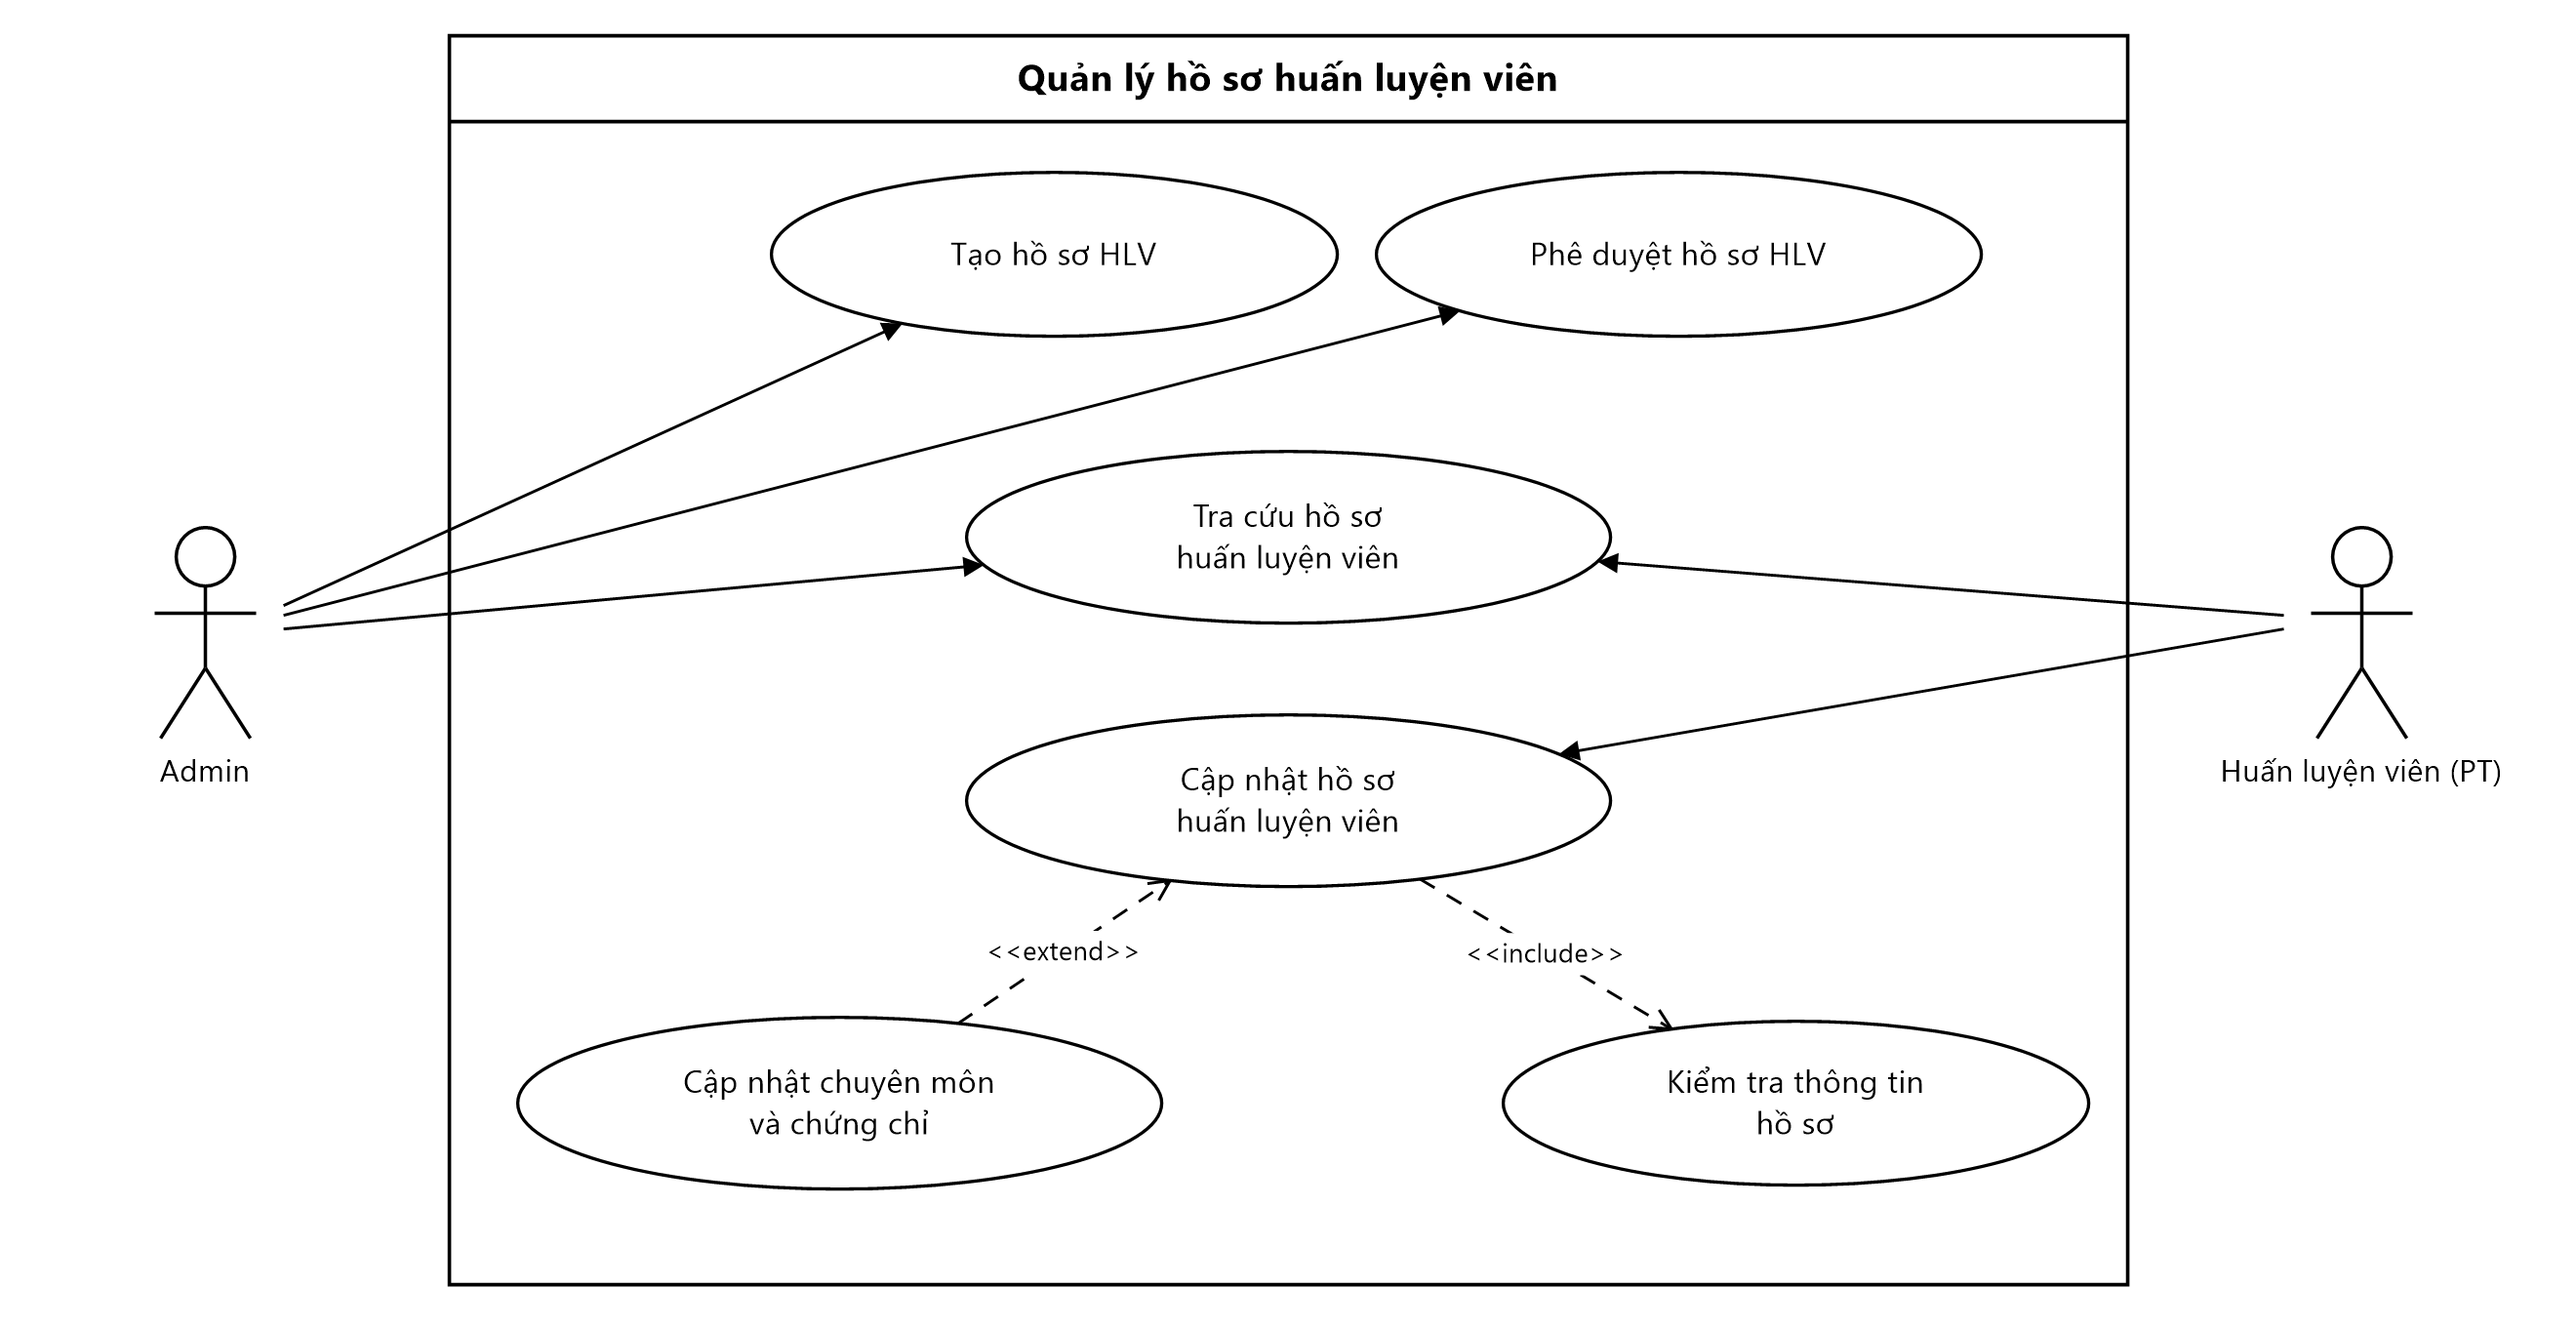
\includegraphics[width=0.88\textwidth, height=0.65\textheight, keepaspectratio]{images/uc_p10_1.png}
\caption{Use-case Quản lý hồ sơ huấn luyện viên}
\end{figure}
\begin{table}[H]\centering\footnotesize
\begin{tabularx}{\textwidth}{|L{3.2cm}|Y|}
\hline \textbf{Tóm tắt} & Cho phép Huấn luyện viên (PT) tra cứu và cập nhật thông tin hồ sơ, chuyên môn, chứng chỉ, chi nhánh giảng dạy; Admin tạo mới, tra cứu và phê duyệt hồ sơ HLV trên hệ thống. \\ \hline
\textbf{Tiền điều kiện} & Người dùng (HLV hoặc Admin) đã đăng nhập thành công với vai trò tương ứng. \\ \hline
\textbf{Dòng sự kiện chính} & 1. Admin hoặc HLV truy cập chức năng quản lý hồ sơ HLV (Admin có thể khởi tạo hoặc tra cứu hồ sơ PT).\newline 2. HLV cập nhật thông tin cá nhân và mở rộng cập nhật chuyên môn, kinh nghiệm, chứng chỉ/bằng cấp, tiểu sử và các chi nhánh giảng dạy.\newline 3. Hệ thống kiểm tra tính đầy đủ, hợp lệ của thông tin hồ sơ.\newline 4. Hệ thống lưu thông tin; đối với hồ sơ mới tạo hoặc thay đổi cần kiểm duyệt, Admin thực hiện phê duyệt để hồ sơ PT sẵn sàng nhận lịch. \\ \hline
\textbf{Dòng sự kiện phụ} & Nếu thông tin bắt buộc bị bỏ trống, số năm kinh nghiệm $< 0$ hoặc chưa chọn ít nhất 1 chi nhánh, hệ thống báo lỗi yêu cầu bổ sung đầy đủ. \\ \hline
\textbf{Hậu điều kiện} & Thông tin hồ sơ chuyên môn của PT được lưu trữ và cập nhật trên hệ thống. \\ \hline
\end{tabularx}
\caption{Bảng đặc tả Use-case 5: Quản lý hồ sơ huấn luyện viên}
\end{table}

\paragraph{6. Tạo \& Gán chi nhánh cho Lễ tân}
\begin{figure}[H]
\centering
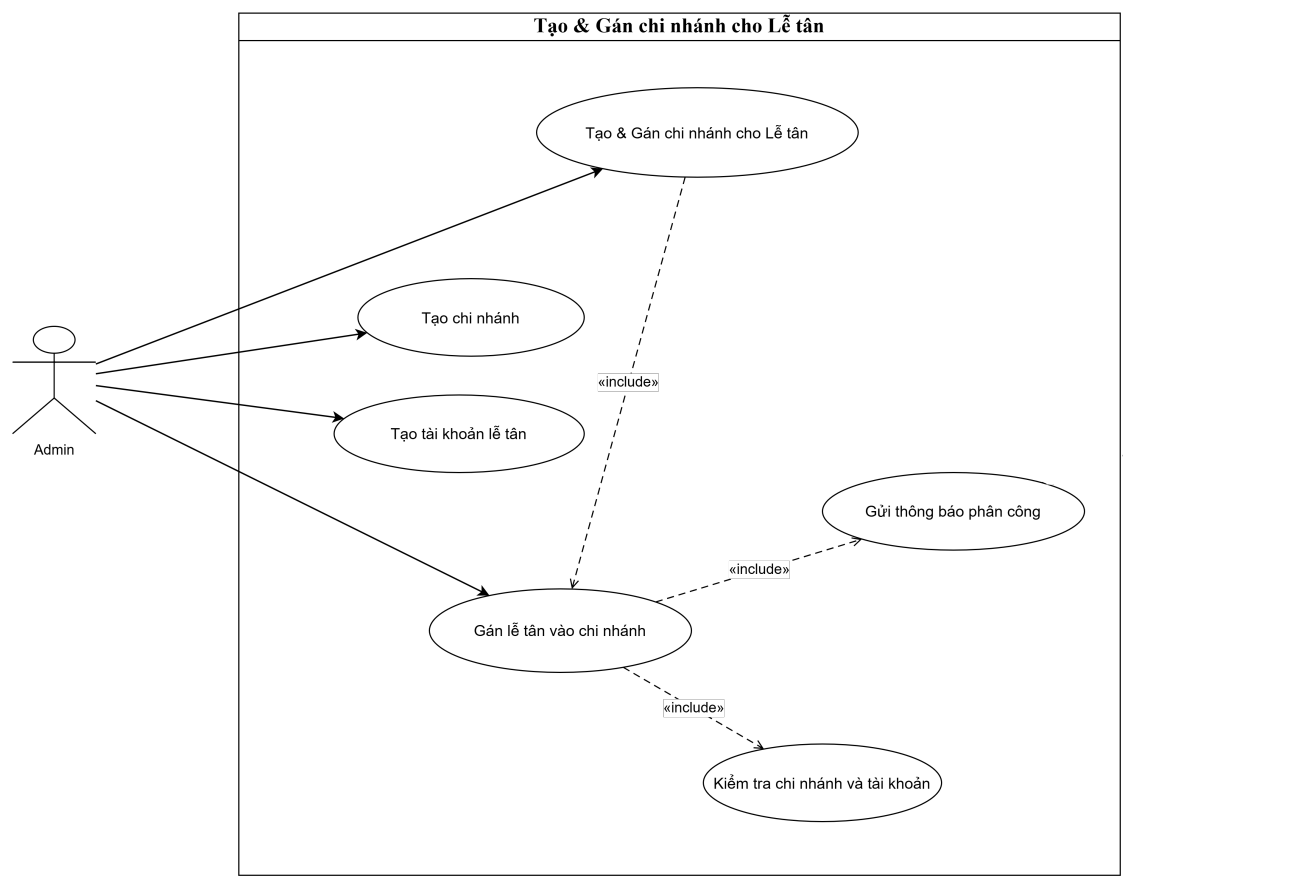
\includegraphics[width=0.88\textwidth, height=0.65\textheight, keepaspectratio]{images/uc_p11_1.png}
\caption{Use-case Tạo \& Gán chi nhánh cho Lễ tân}
\end{figure}
\begin{table}[H]\centering\footnotesize
\begin{tabularx}{\textwidth}{|L{3.2cm}|Y|}
\hline \textbf{Tóm tắt} & Admin khởi tạo tài khoản làm việc cho Nhân viên Lễ tân mới và chỉ định chi nhánh trực thuộc hoạt động. \\ \hline
\textbf{Tiền điều kiện} & Admin đăng nhập bằng tài khoản quản trị và có nhu cầu bổ sung/thay đổi nhân sự lễ tân. \\ \hline
\textbf{Dòng sự kiện chính} & 1. Admin nhập thông tin nhân viên lễ tân mới (Họ tên, Email, Số điện thoại).\newline 2. Admin chọn vai trò \texttt{Staff} (Lễ tân) và chọn Chi nhánh làm việc cụ thể.\newline 3. Hệ thống tạo tài khoản mới và tự động gán quyền làm việc tại chi nhánh đã chọn.\newline 4. Hệ thống gọi Use-case "Gửi thông báo" để gửi thông tin đăng nhập/mật khẩu khởi tạo tới Email của lễ tân. \\ \hline
\textbf{Dòng sự kiện phụ} & Nếu Email/SĐT trùng lặp, hệ thống báo lỗi và hủy quá trình tạo. \\ \hline
\textbf{Hậu điều kiện} & Tài khoản Lễ tân được kích hoạt và gán đúng chi nhánh làm việc. \\ \hline
\end{tabularx}
\caption{Bảng đặc tả Use-case 6: Tạo \& Gán chi nhánh cho Lễ tân}
\end{table}

\paragraph{7. Quản lý phân quyền \& Khóa/Mở khóa tài khoản}
\begin{figure}[H]
\centering
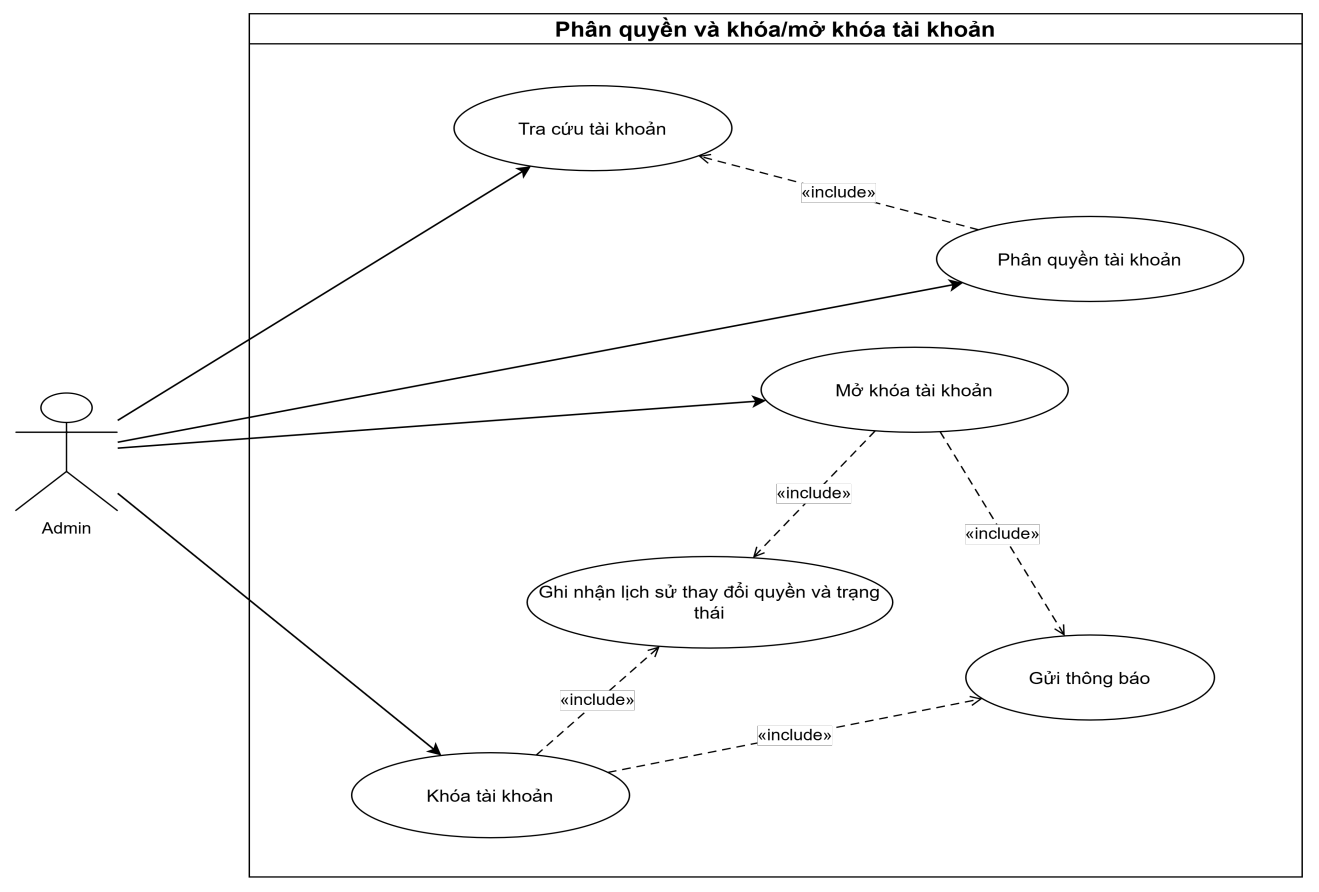
\includegraphics[width=0.88\textwidth, height=0.65\textheight, keepaspectratio]{images/uc_p12_1.png}
\caption{Use-case Quản lý phân quyền \& Khóa/Mở khóa tài khoản}
\end{figure}
\begin{table}[H]\centering\footnotesize
\begin{tabularx}{\textwidth}{|L{3.2cm}|Y|}
\hline \textbf{Tóm tắt} & Admin xem toàn bộ danh sách người dùng, cập nhật/thay đổi vai trò phân quyền hoặc thực hiện khóa/mở khóa tài khoản khi cần thiết. \\ \hline
\textbf{Tiền điều kiện} & Admin đăng nhập vào trang quản trị hệ thống. \\ \hline
\textbf{Dòng sự kiện chính} & 1. Admin xem danh sách tổng hợp tất cả các tài khoản người dùng (Hội viên, PT, Lễ tân).\newline 2. Admin chọn một tài khoản cụ thể để thay đổi vai trò / phân lại quyền hạn, hoặc chuyển trạng thái giữa "Hoạt động" (Active) và "Bị khóa" (Locked).\newline 3. Hệ thống lưu cập nhật vào cơ sở dữ liệu.\newline 4. Hệ thống tự động gọi Use-case "Gửi thông báo" để thông báo cho người dùng. \\ \hline
\textbf{Dòng sự kiện phụ} & Nếu tài khoản bị khóa, các phiên làm việc hiện tại của tài khoản đó lập tức bị hủy và không thể đăng nhập lại cho đến khi được mở khóa. \\ \hline
\textbf{Hậu điều kiện} & Trạng thái tài khoản hoặc phân quyền người dùng được cập nhật chính xác trên toàn hệ thống. \\ \hline
\end{tabularx}
\caption{Bảng đặc tả Use-case 7: Quản lý phân quyền \& Khóa/Mở khóa tài khoản}
\end{table}

\paragraph{8. Mua gói tập}
\begin{figure}[H]
\centering
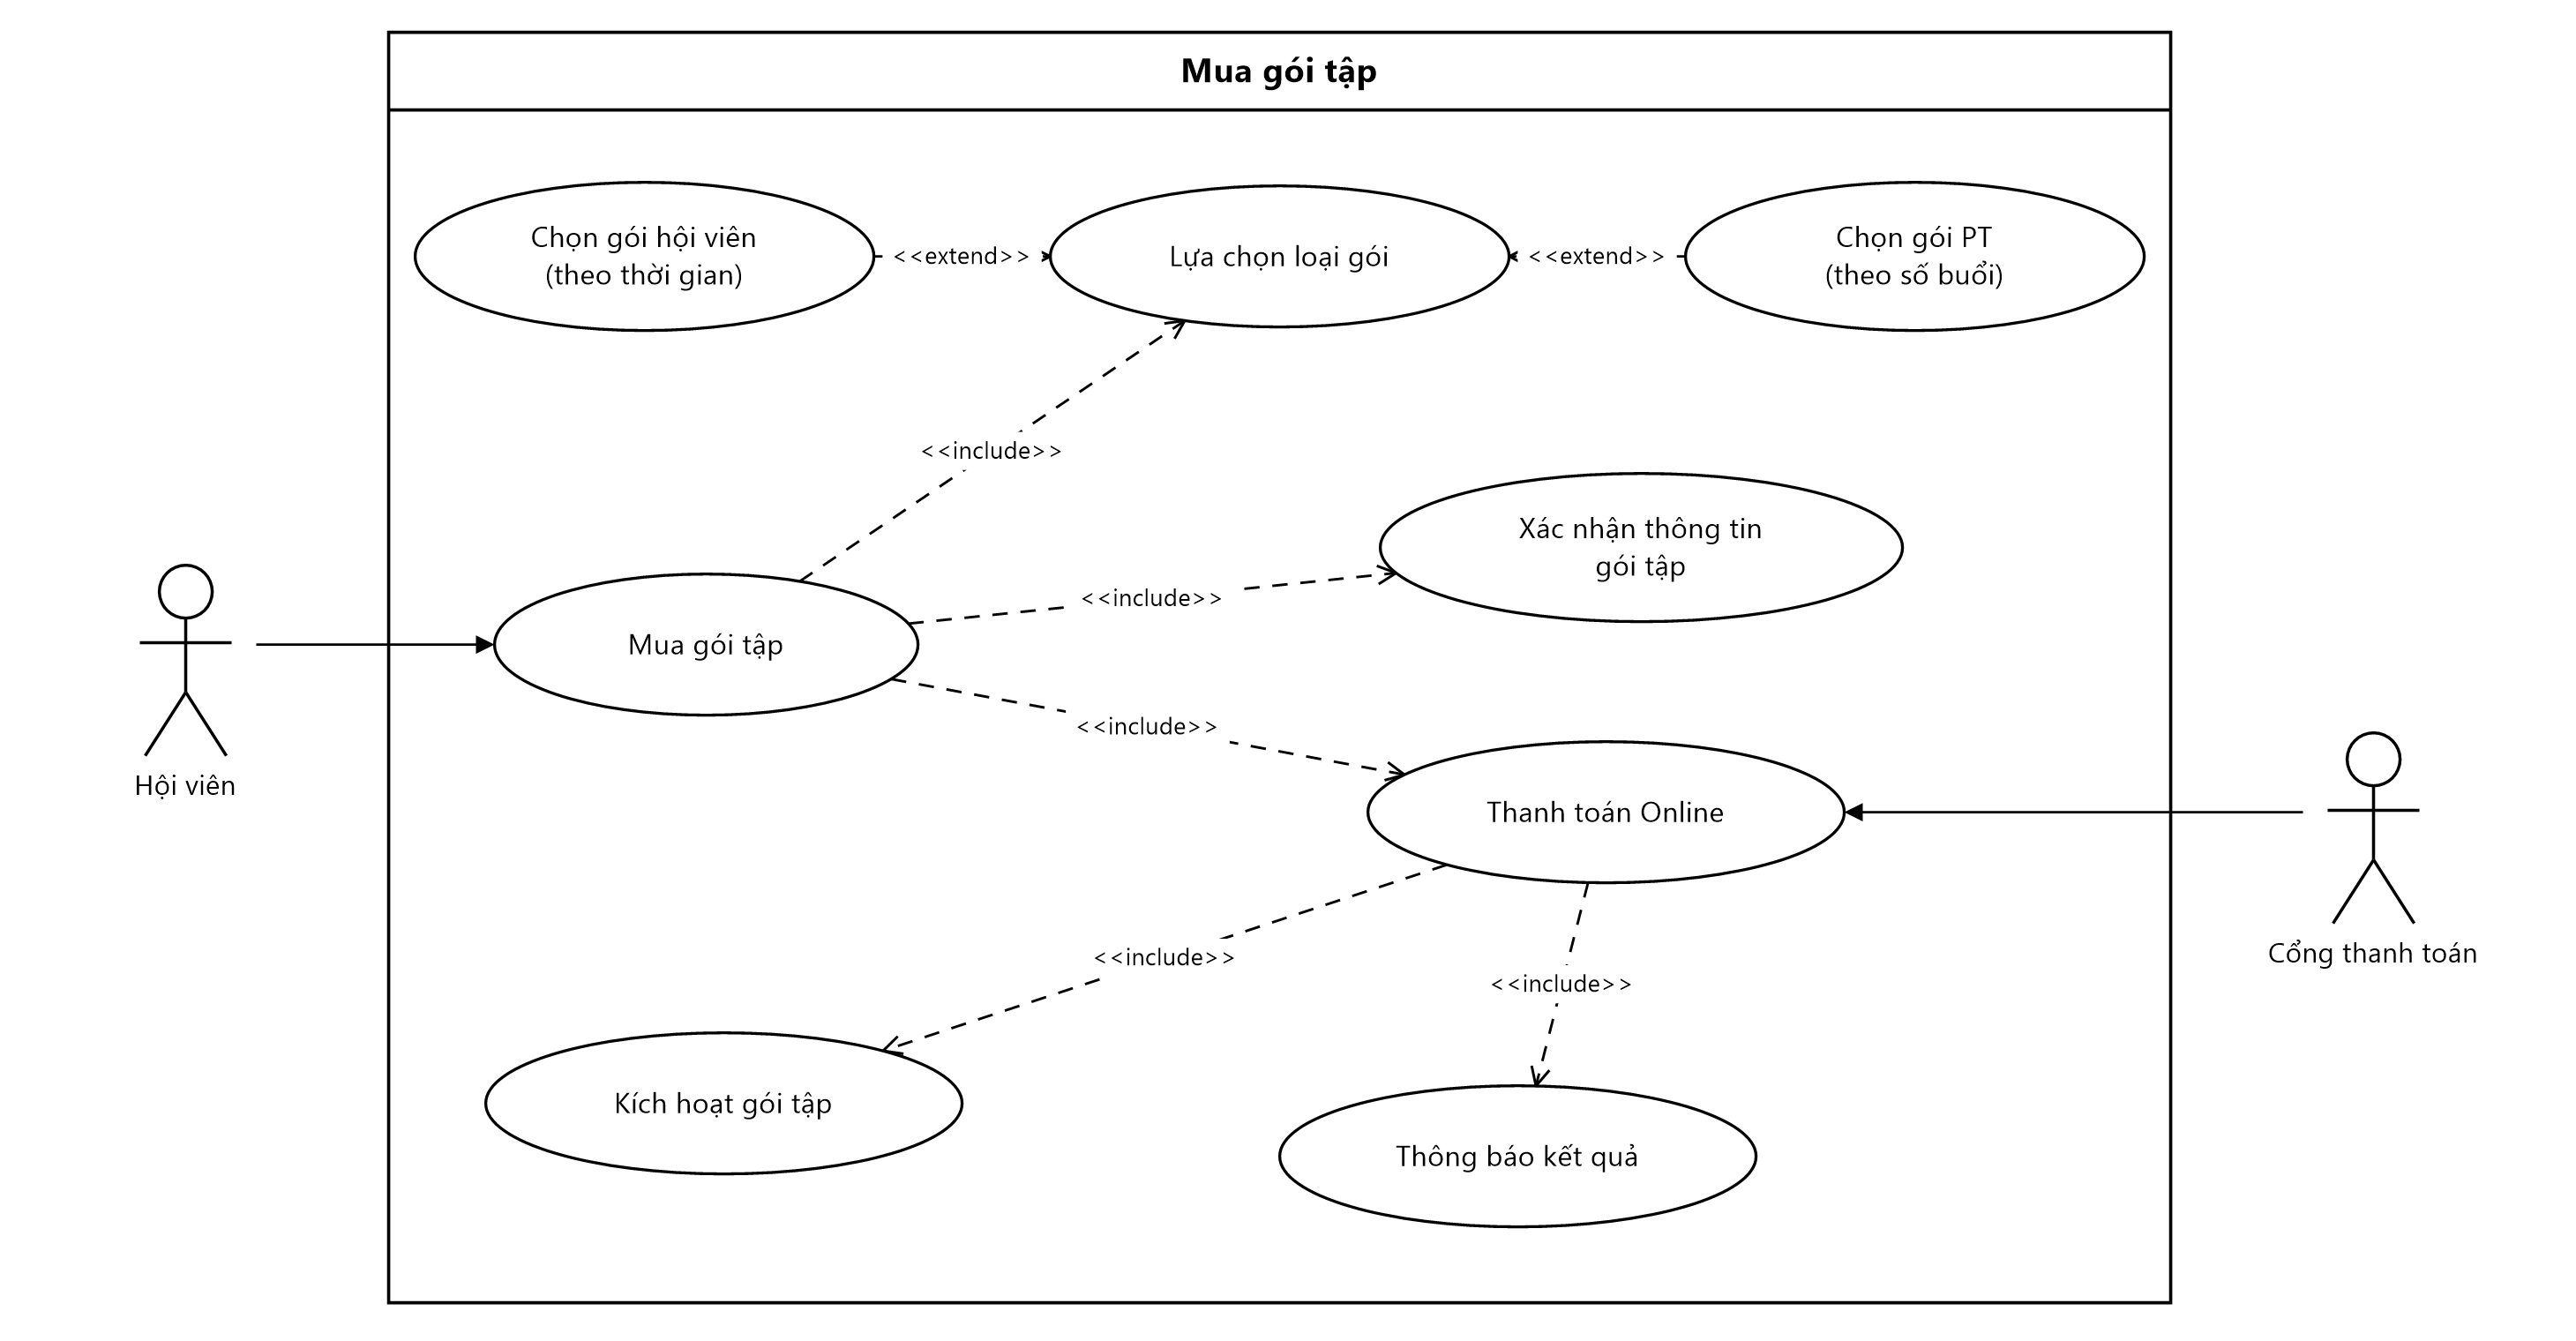
\includegraphics[width=0.88\textwidth, height=0.65\textheight, keepaspectratio]{images/uc_p13_1.png}
\caption{Use-case Mua gói tập}
\end{figure}
\begin{table}[H]\centering\footnotesize
\begin{tabularx}{\textwidth}{|L{3.2cm}|Y|}
\hline \textbf{Tóm tắt} & Hội viên lựa chọn gói hội viên (theo thời hạn) hoặc gói PT (theo số buổi) và thực hiện quy trình mua gói trên hệ thống. \\ \hline
\textbf{Tiền điều kiện} & Hội viên đã đăng ký, đăng nhập thành công và chưa có gói tập phù hợp hoặc muốn mua thêm gói mới. \\ \hline
\textbf{Dòng sự kiện chính} & 1. Hội viên xem danh mục các gói tập (gói thời hạn, gói VIP kèm buổi PT, hoặc gói PT 1-kèm-1).\newline 2. Hội viên chọn gói tập muốn mua và bấm chọn thanh toán.\newline 3. Hệ thống gọi Use-case "Thanh toán Online" kết nối tới tác nhân Cổng thanh toán.\newline 4. Sau khi Cổng thanh toán xác nhận thành công, hệ thống ghi nhận và kích hoạt gói tập mới cho hội viên. \\ \hline
\textbf{Dòng sự kiện phụ} & Để mua được gói PT 1-kèm-1, hội viên phải đang sở hữu một gói hội viên còn hiệu lực. Nếu gói hội viên hết hạn, hệ thống đưa ra cảnh báo và yêu cầu mua/gia hạn gói hội viên trước. \\ \hline
\textbf{Hậu điều kiện} & Thông tin giao dịch được ghi nhận và chuyển tiếp sang kích hoạt gói tập. \\ \hline
\end{tabularx}
\caption{Bảng đặc tả Use-case 8: Mua gói tập}
\end{table}

\paragraph{9. Gia hạn gói tập}
\begin{figure}[H]
\centering
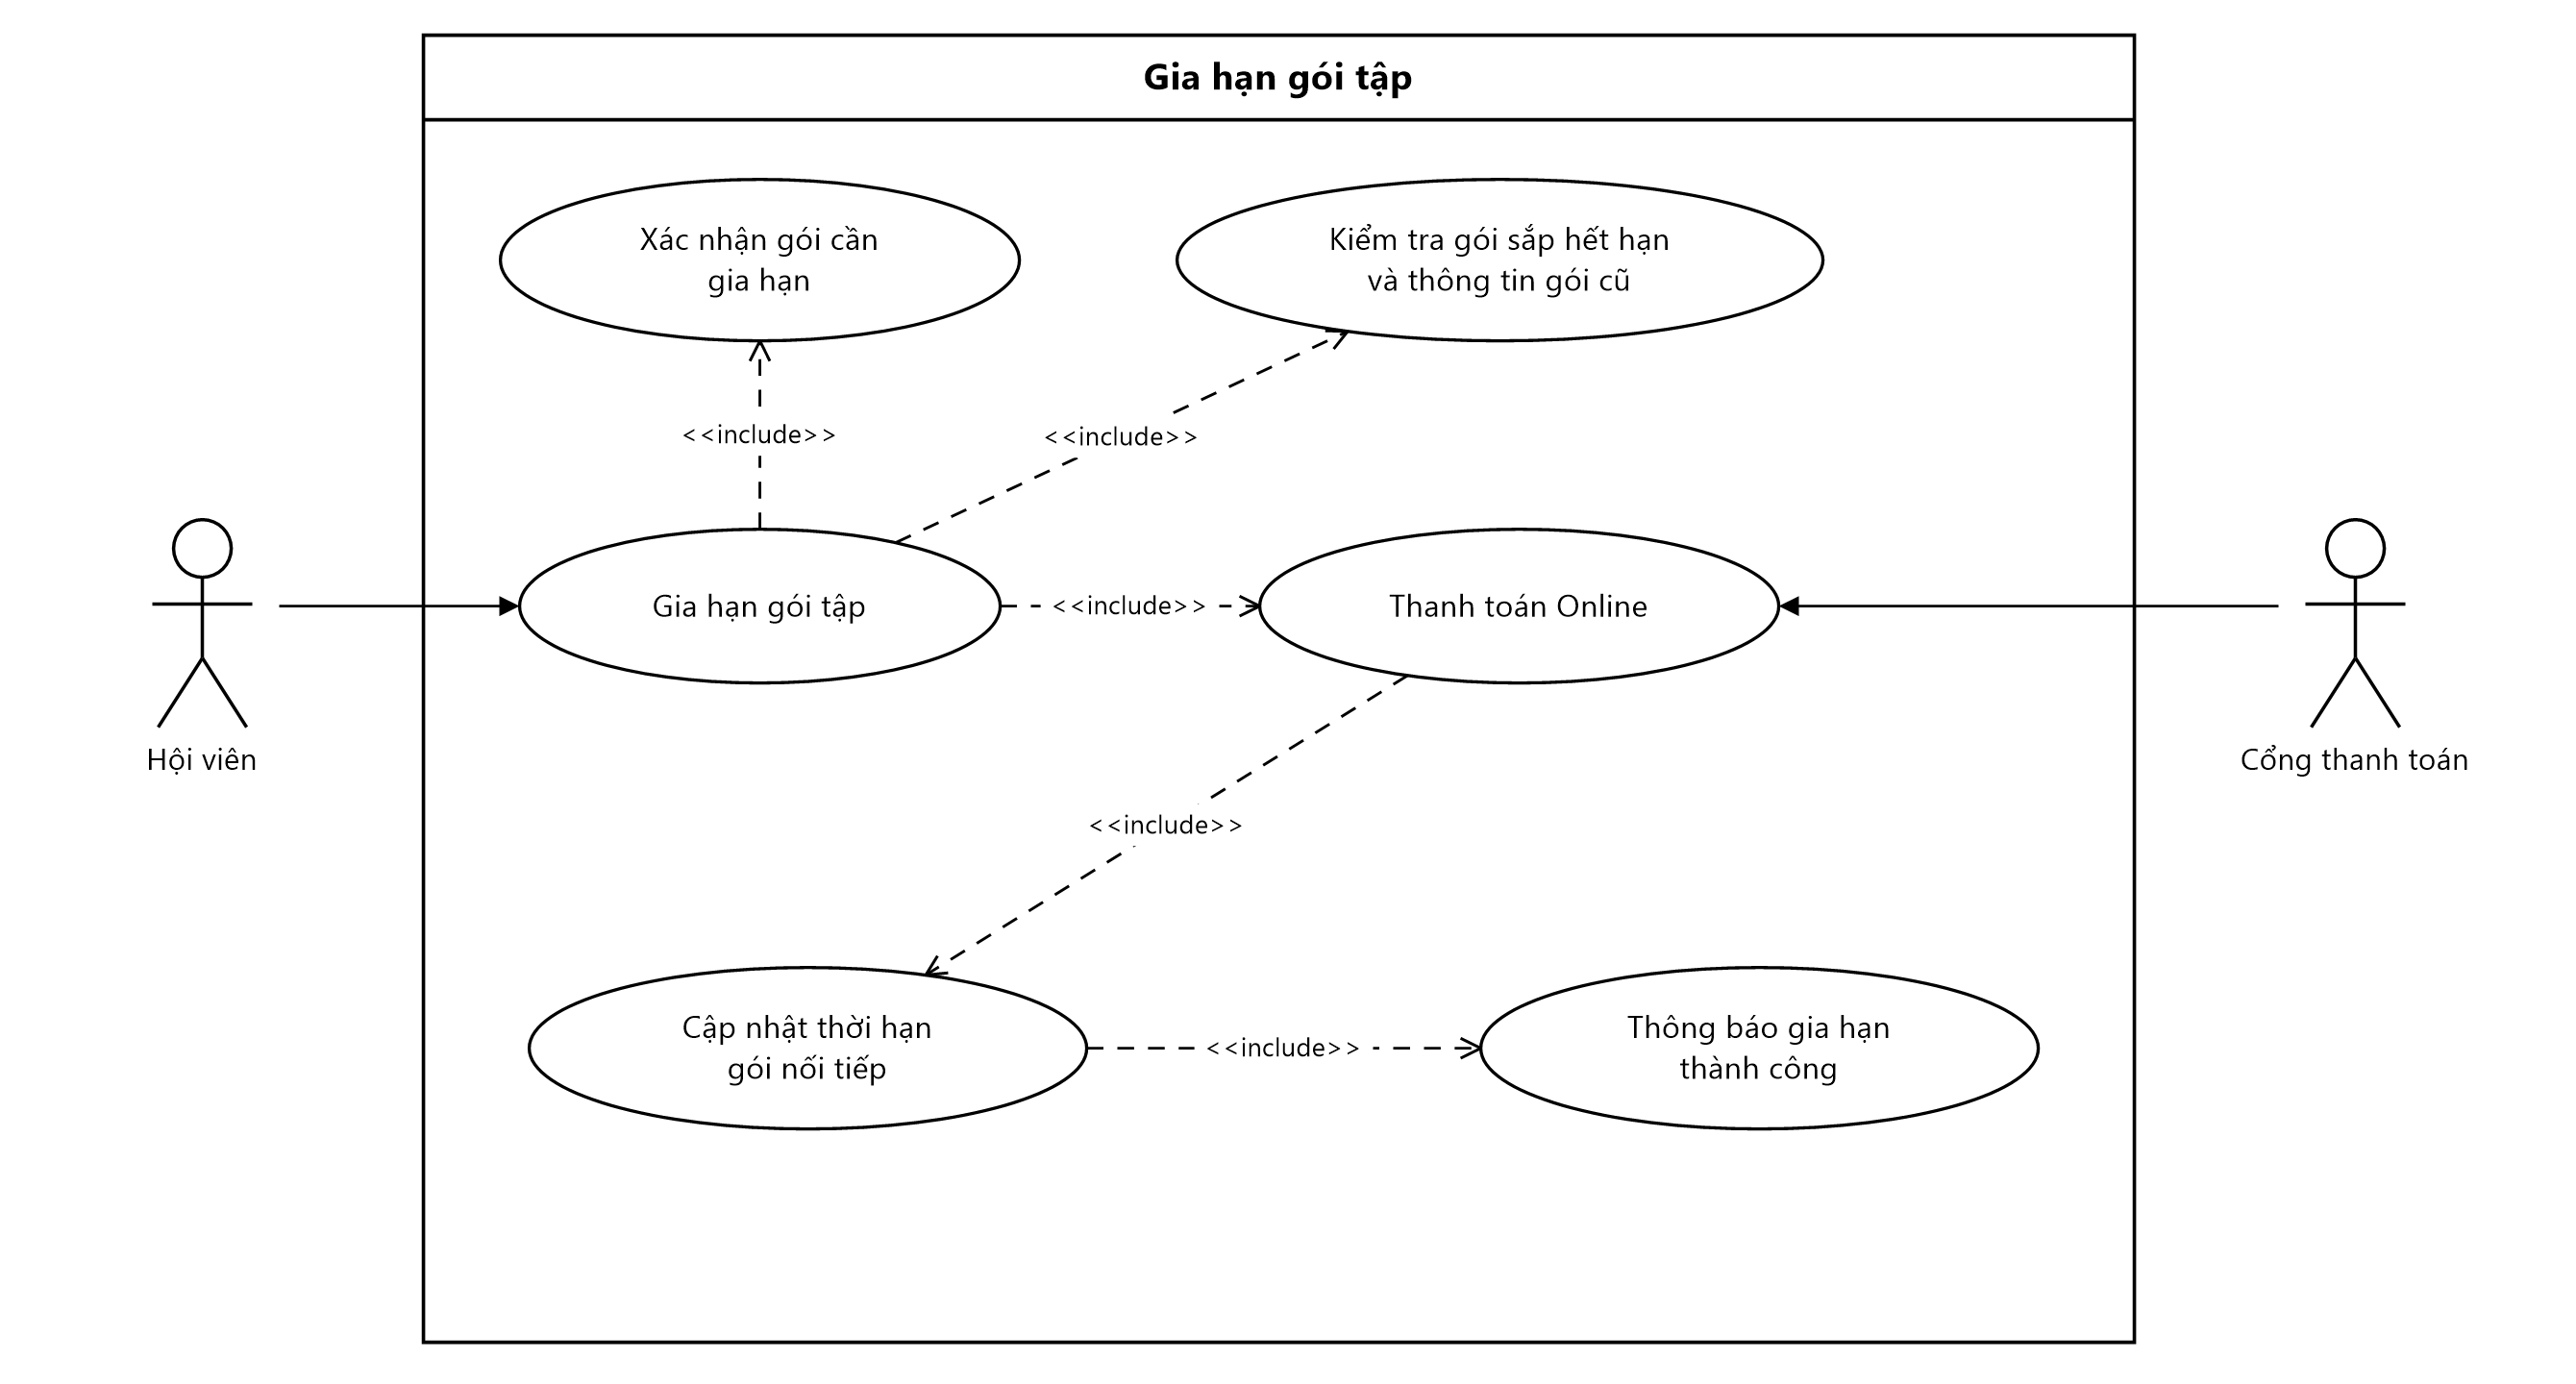
\includegraphics[width=0.88\textwidth, height=0.65\textheight, keepaspectratio]{images/uc_p14_1.png}
\caption{Use-case Gia hạn gói tập}
\end{figure}
\begin{table}[H]\centering\footnotesize
\begin{tabularx}{\textwidth}{|L{3.2cm}|Y|}
\hline \textbf{Tóm tắt} & Hội viên thực hiện gia hạn gói tập khi gói hiện tại gần hết hạn, thời gian sử dụng mới được tự động cộng nối tiếp. \\ \hline
\textbf{Tiền điều kiện} & Hội viên đang sở hữu gói tập đang hoạt động hoặc sắp hết hạn và đủ điều kiện gia hạn. \\ \hline
\textbf{Dòng sự kiện chính} & 1. Hội viên chọn chức năng gia hạn gói tập đang dùng.\newline 2. Hệ thống tính toán thời gian gia hạn: Ngày bắt đầu gói mới được tính nối tiếp từ ngày hết hạn của gói cũ.\newline 3. Hệ thống hiển thị số tiền cần thanh toán và gọi Use-case "Thanh toán Online" kết nối tới tác nhân Cổng thanh toán.\newline 4. Khi Cổng thanh toán phản hồi thành công, hệ thống cập nhật ngày hết hạn mới cho gói tập. \\ \hline
\textbf{Dòng sự kiện phụ} & Nếu hội viên gia hạn khi gói đã hết hạn quá lâu, hệ thống tính ngày kích hoạt gói mới từ thời điểm thanh toán thành công thay vì nối tiếp. \\ \hline
\textbf{Hậu điều kiện} & Hạn sử dụng của gói tập được cập nhật nối tiếp thành công. \\ \hline
\end{tabularx}
\caption{Bảng đặc tả Use-case 9: Gia hạn gói tập}
\end{table}

\paragraph{10. Thanh toán Online}
\begin{figure}[H]
\centering
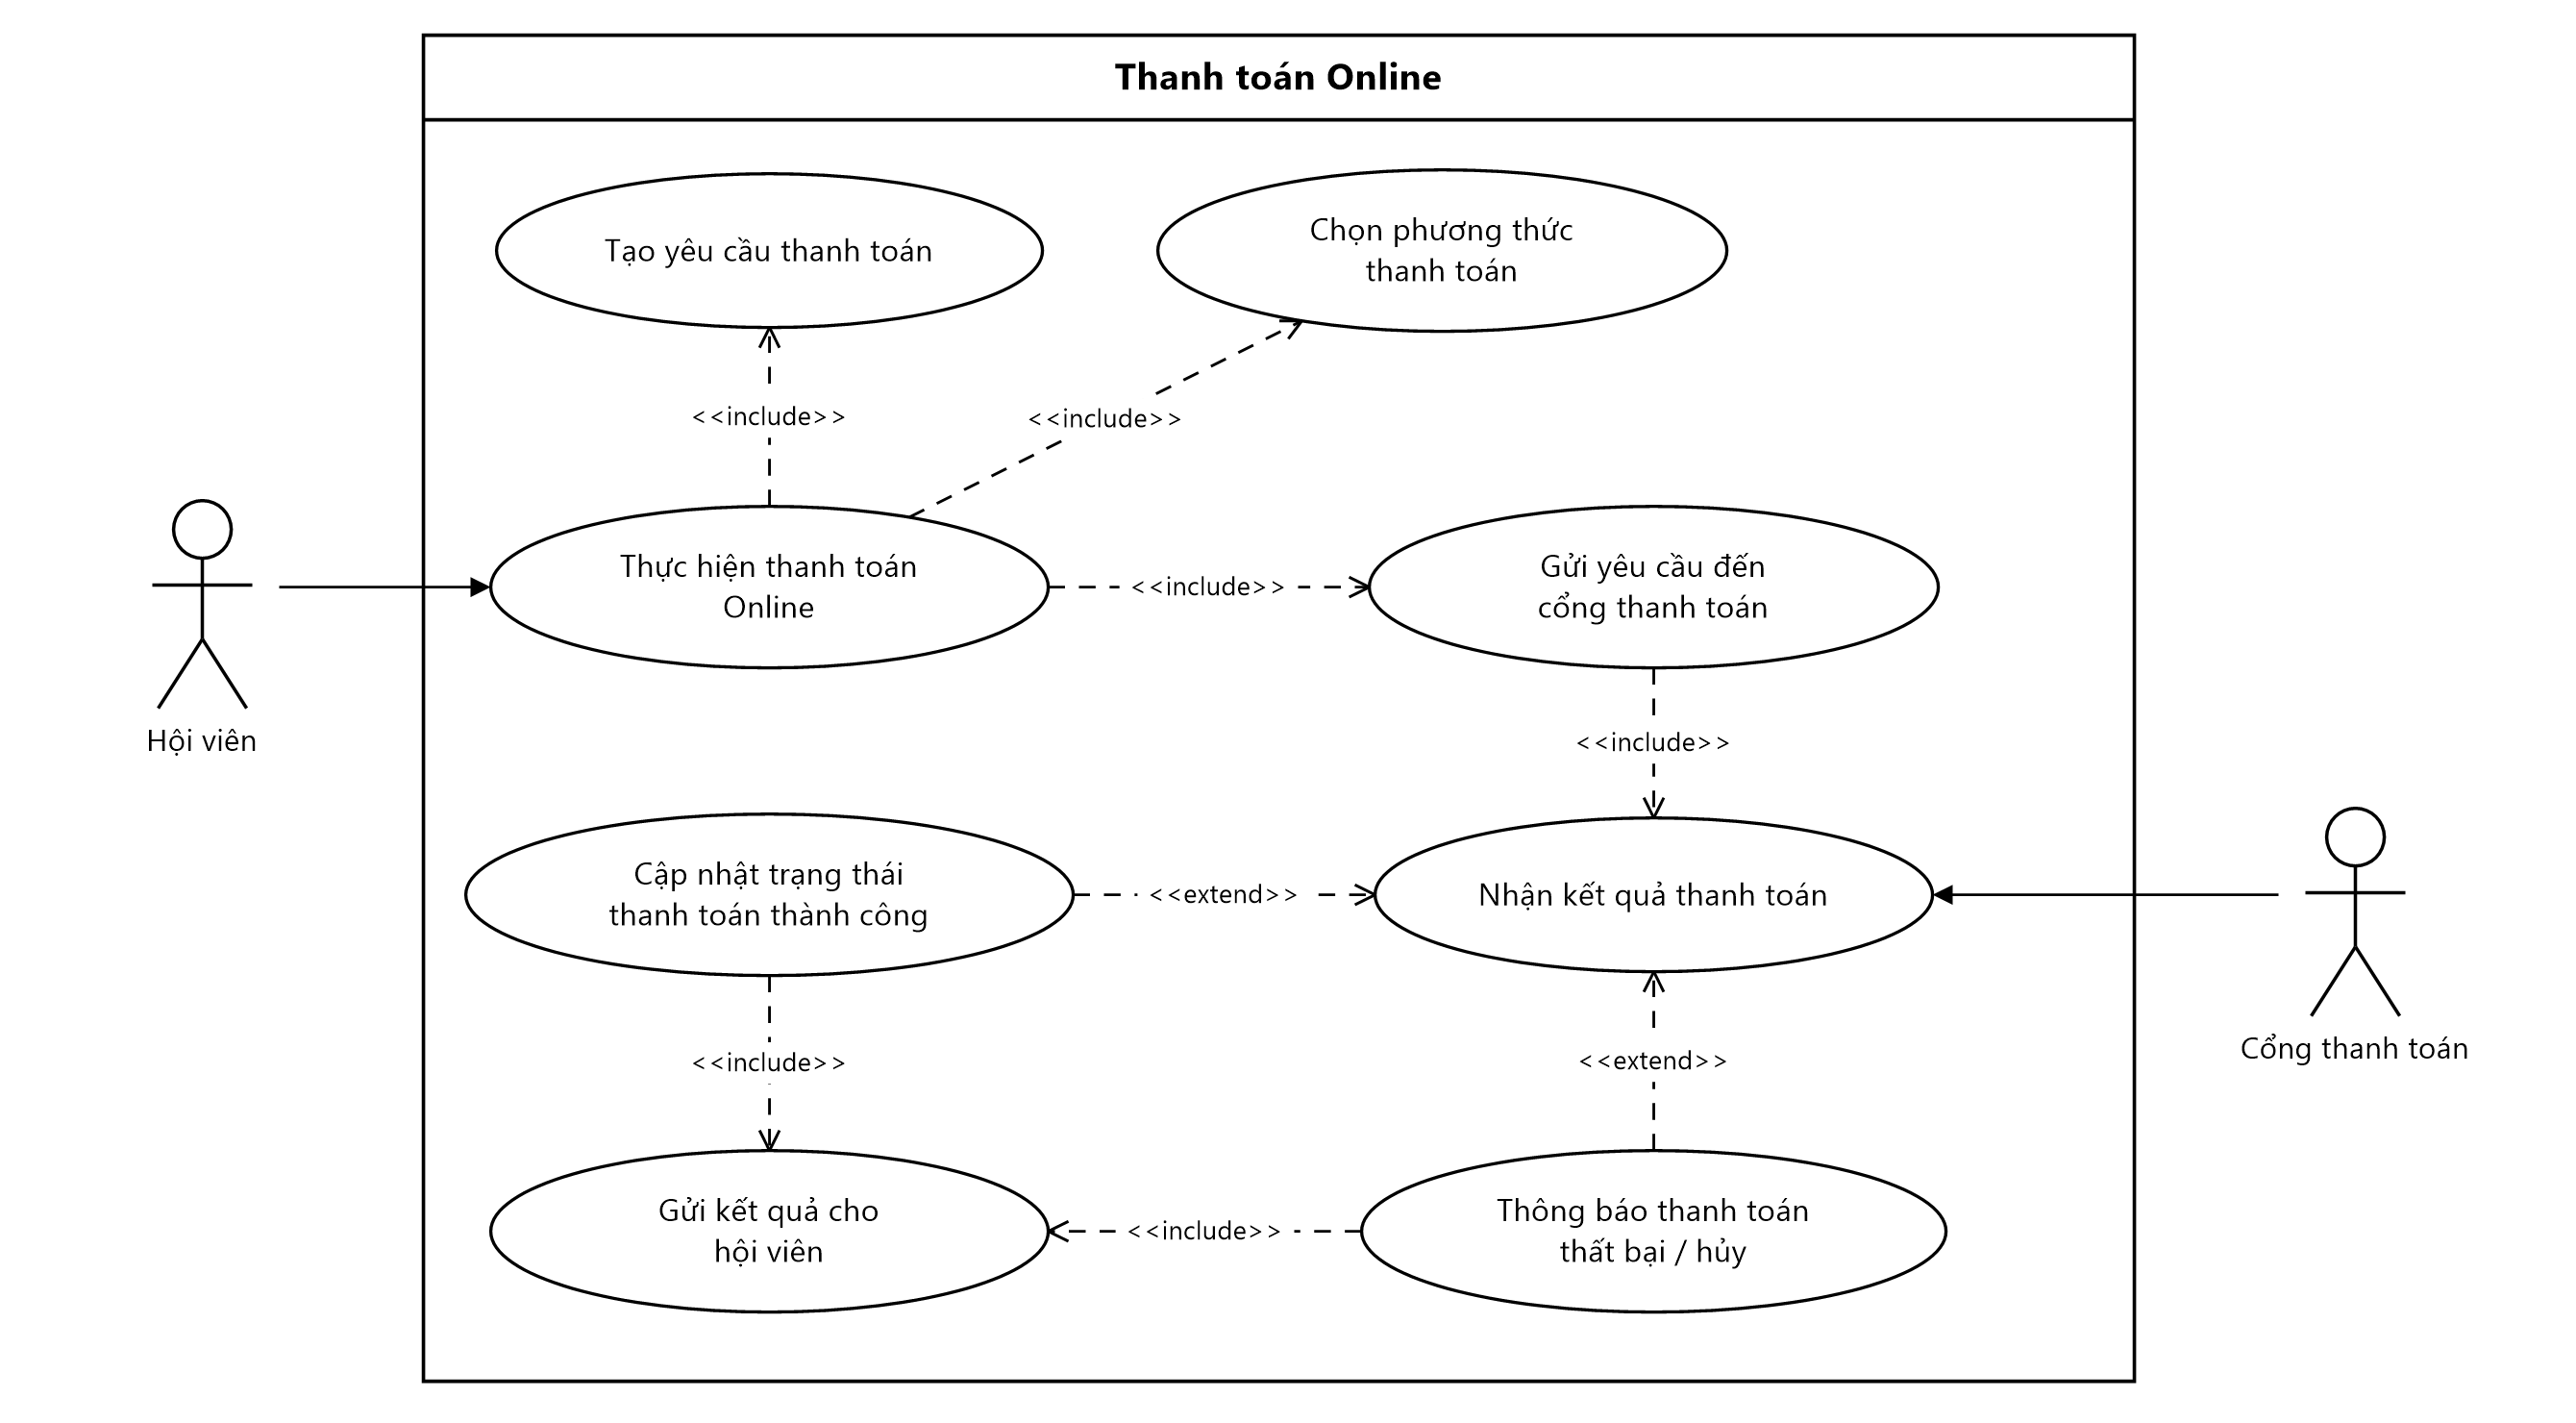
\includegraphics[width=0.88\textwidth, height=0.65\textheight, keepaspectratio]{images/uc_p15_1.png}
\caption{Use-case Thanh toán Online}
\end{figure}
\begin{table}[H]\centering\footnotesize
\begin{tabularx}{\textwidth}{|L{3.2cm}|Y|}
\hline \textbf{Tóm tắt} & Hệ thống phối hợp với tác nhân hệ thống Cổng thanh toán (VNPay / ZaloPay) để xử lý giao dịch tài chính cho việc mua mới hoặc gia hạn gói tập. \\ \hline
\textbf{Tiền điều kiện} & Có yêu cầu thanh toán phát sinh từ Use-case "Mua gói tập" hoặc "Gia hạn gói tập". \\ \hline
\textbf{Dòng sự kiện chính} & 1. Hệ thống tạo đơn hàng, ghi nhận mã giao dịch và chuyển yêu cầu sang giao diện của Cổng thanh toán.\newline 2. Hội viên nhập thông tin và xác thực thanh toán trực tiếp trên Cổng thanh toán.\newline 3. Cổng thanh toán gửi kết quả giao dịch (callback) về cho hệ thống.\newline 4. Nếu giao dịch thành công, hệ thống ghi nhận trạng thái "Thành công" và tự động kích hoạt/gia hạn gói tập. \\ \hline
\textbf{Dòng sự kiện phụ} & Nếu thanh toán thất bại (không đủ số dư, hủy giao dịch, lỗi cổng), hệ thống lưu trạng thái "Thất bại", gọi Use-case "Gửi thông báo" để báo lỗi và cho phép thanh toán lại. \\ \hline
\textbf{Hậu điều kiện} & Kết quả giao dịch (Thành công/Thất bại) được ghi nhận chính xác vào lịch sử giao dịch. \\ \hline
\end{tabularx}
\caption{Bảng đặc tả Use-case 10: Thanh toán Online}
\end{table}

\paragraph{11. Quản lý \& Đặt lịch Lớp học nhóm}
\begin{figure}[H]
\centering
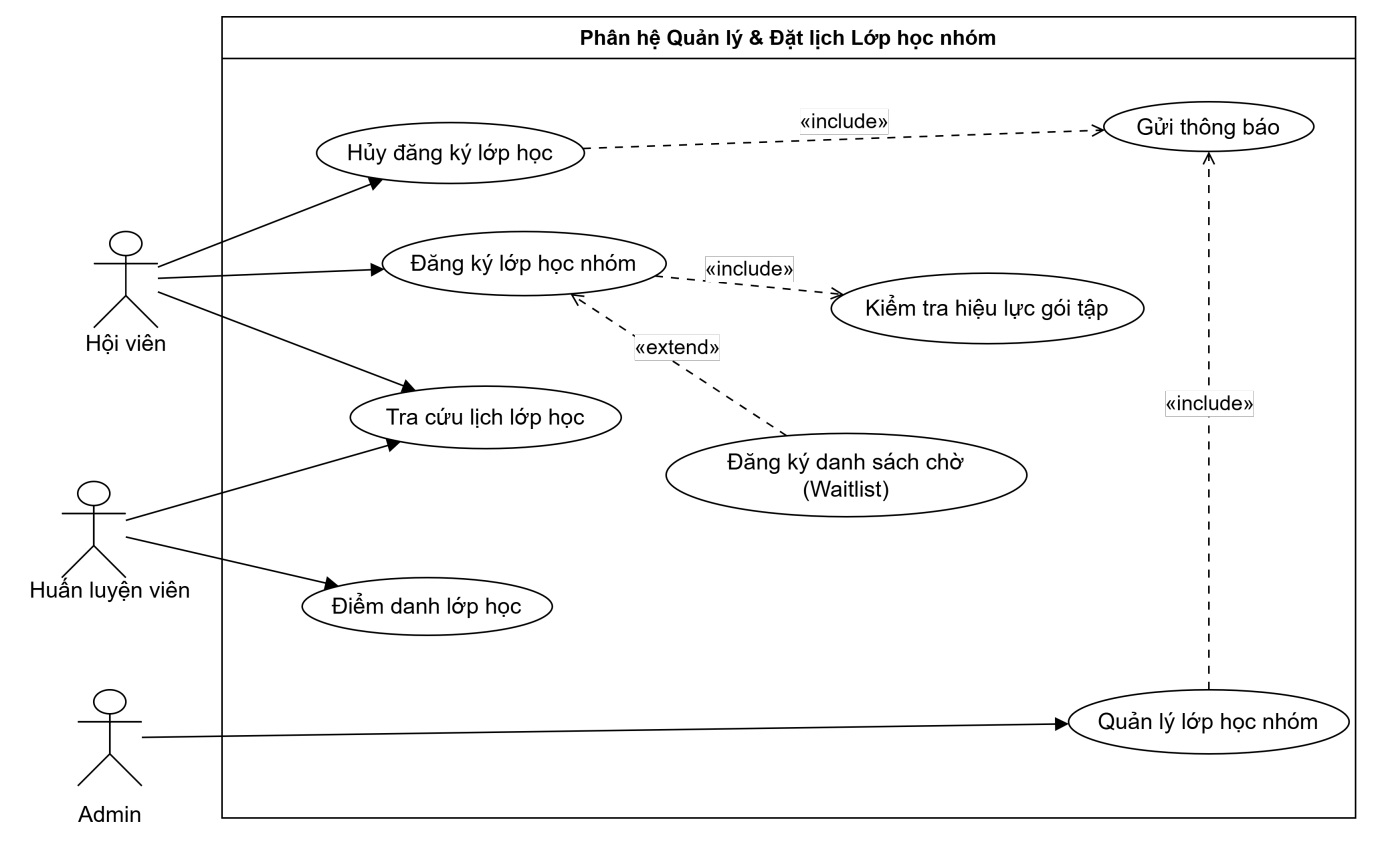
\includegraphics[width=0.88\textwidth, height=0.65\textheight, keepaspectratio]{images/uc_p16_1.png}
\caption{Use-case Quản lý \& Đặt lịch Lớp học nhóm}
\end{figure}

\begin{table}[H]\centering\footnotesize
\begin{tabularx}{\textwidth}{|L{3.2cm}|Y|}
\hline \textbf{Tóm tắt} & Cho phép Admin tạo lớp học mới, phân công HLV, cập nhật thông tin hoặc hủy/đổi lịch một buổi học cụ thể và gửi thông báo cho các bên liên quan. \\ \hline
\textbf{Tiền điều kiện} & Admin đã đăng nhập; dữ liệu về Chi nhánh, Phòng tập và Huấn luyện viên đã có sẵn. \\ \hline
\textbf{Dòng sự kiện chính} & 1. Admin chọn "Quản lý lớp học nhóm" $\rightarrow$ "Tạo lớp mới".\newline 2. Nhập tên lớp, chi nhánh, phòng tập, khung giờ lặp lại, sĩ số tối đa và chọn HLV phụ trách.\newline 3. Hệ thống kiểm tra xung đột lịch phòng tập và lịch dạy của HLV.\newline 4. Lưu thông tin lớp, khởi tạo danh sách buổi học định kỳ và gửi thông báo phân công cho HLV. \\ \hline
\textbf{Dòng sự kiện phụ} & -- Đổi lịch buổi học: cập nhật thời gian/HLV mới và gửi thông báo cho HLV và hội viên.\newline -- Hủy buổi học: chuyển trạng thái "Đã hủy", hoàn lại lượt đặt cho hội viên và gửi thông báo.\newline -- Trùng lịch phòng/HLV: báo lỗi yêu cầu chọn khung giờ hoặc HLV khác. \\ \hline
\textbf{Hậu điều kiện} & Thông tin lớp học nhóm và lịch dạy được cập nhật thành công, sẵn sàng cho hội viên tra cứu và đặt lịch. \\ \hline
\end{tabularx}
\caption{Bảng đặc tả Use-case 11: Quản lý lớp học nhóm}
\end{table}

\begin{table}[H]\centering\footnotesize
\begin{tabularx}{\textwidth}{|L{3.2cm}|Y|}
\hline \textbf{Tóm tắt} & Hội viên chọn đăng ký tham gia một buổi học nhóm; hệ thống kiểm tra hiệu lực gói tập và xếp chỗ chính thức hoặc đưa vào danh sách chờ (Waitlist) nếu lớp đã đầy. \\ \hline
\textbf{Tiền điều kiện} & Hội viên đã đăng nhập; buổi học nhóm đang mở đăng ký (chưa diễn ra và không bị hủy). \\ \hline
\textbf{Dòng sự kiện chính} & 1. Hội viên tra cứu và chọn buổi học nhóm muốn tham gia, nhấn "Đăng ký".\newline 2. Hệ thống kiểm tra gói hội viên (còn hạn, không freeze, đúng chi nhánh, còn lượt đặt).\newline 3. Kiểm tra sĩ số lớp còn chỗ trống và hội viên không bị trùng lịch.\newline 4. Ghi nhận đăng ký trạng thái "Đã xác nhận", trừ 1 lượt đặt và gửi thông báo xác nhận. \\ \hline
\textbf{Dòng sự kiện phụ} & -- Lớp đầy và còn $> 8$ tiếng: đề nghị vào Waitlist theo thứ tự ưu tiên gói tập và thời điểm đăng ký.\newline -- Lớp đầy và còn $< 8$ tiếng: không nhận thêm Waitlist, yêu cầu chọn lớp khác.\newline -- Gói tập không hợp lệ: từ chối đăng ký và thông báo lý do. \\ \hline
\textbf{Hậu điều kiện} & Hội viên được thêm vào danh sách lớp chính thức (hoặc Waitlist), hoặc giữ nguyên trạng thái nếu từ chối. \\ \hline
\end{tabularx}
\caption{Bảng đặc tả Use-case 12: Đăng ký lớp học nhóm}
\end{table}

\begin{table}[H]\centering\footnotesize
\begin{tabularx}{\textwidth}{|L{3.2cm}|Y|}
\hline \textbf{Tóm tắt} & Hội viên hủy buổi học nhóm đã đặt; hệ thống xét hoàn lượt nếu đúng hạn và tự động đôn hội viên từ Waitlist (nếu có) vào lớp. \\ \hline
\textbf{Tiền điều kiện} & Hội viên đã đăng nhập và có lịch đặt lớp nhóm chưa diễn ra. \\ \hline
\textbf{Dòng sự kiện chính} & 1. Hội viên chọn buổi học muốn hủy và nhấn "Hủy đăng ký".\newline 2. Hệ thống kiểm tra thời điểm hủy nằm trước thời hạn quy định và yêu cầu xác nhận.\newline 3. Cập nhật trạng thái "Đã hủy" và hoàn lại 1 lượt đặt lớp.\newline 4. Nếu có Waitlist (và còn $> 8$ tiếng), tự động đôn người ưu tiên cao nhất vào lớp và gửi thông báo. \\ \hline
\textbf{Dòng sự kiện phụ} & -- Hủy quá hạn: cảnh báo mất lượt; nếu tiếp tục hủy thì không hoàn lượt.\newline -- Hủy tự động khi duyệt Freeze: tự động hủy các lịch trong khoảng freeze và hoàn lượt.\newline -- Đóng Waitlist trước 8 tiếng: thông báo cho các hội viên còn chờ chọn lớp khác. \\ \hline
\textbf{Hậu điều kiện} & Lịch đặt bị hủy; sĩ số lớp và danh sách chờ (Waitlist) được cập nhật chính xác. \\ \hline
\end{tabularx}
\caption{Bảng đặc tả Use-case 13: Hủy đăng ký lớp học}
\end{table}

\begin{table}[H]\centering\footnotesize
\begin{tabularx}{\textwidth}{|L{3.2cm}|Y|}
\hline \textbf{Tóm tắt} & HLV điểm danh hội viên tham gia buổi học nhóm; hệ thống đối chiếu cờ đã check-in tại chi nhánh trong ngày để HLV chốt trạng thái tham gia và mở quyền đánh giá. \\ \hline
\textbf{Tiền điều kiện} & HLV đã đăng nhập, được phân công dạy buổi học; buổi học đã bắt đầu hoặc vừa kết thúc. \\ \hline
\textbf{Dòng sự kiện chính} & 1. HLV chọn buổi học và mở chức năng "Điểm danh".\newline 2. Hệ thống hiển thị danh sách học viên đã đăng ký kèm cờ trạng thái đã check-in tại chi nhánh trong ngày.\newline 3. HLV tích xác nhận "Có mặt" (đối với học viên đã check-in hợp lệ) hoặc "Vắng mặt" (\texttt{No\_Show}) và nhấn "Lưu điểm danh".\newline 4. Hệ thống cập nhật trạng thái tham gia và mở quyền đánh giá cho các hội viên được xác nhận có mặt. \\ \hline
\textbf{Dòng sự kiện phụ} & -- Chưa check-in: không cho xác nhận "Có mặt" (hệ thống từ chối hoặc yêu cầu check-in tại quầy trước).\newline -- Vắng mặt: ghi nhận \texttt{No\_Show}, lượt đặt vẫn tính đã sử dụng và không mở quyền đánh giá. \\ \hline
\textbf{Hậu điều kiện} & Dữ liệu điểm danh được lưu trữ để tính hiệu suất lớp/HLV; hội viên tham gia hợp lệ được mở quyền đánh giá. \\ \hline
\end{tabularx}
\caption{Bảng đặc tả Use-case 14: Điểm danh lớp học}
\end{table}

\begin{table}[H]\centering\footnotesize
\begin{tabularx}{\textwidth}{|L{3.2cm}|Y|}
\hline \textbf{Tóm tắt} & Hội viên hoặc HLV xem thời khóa biểu các lớp học nhóm theo bộ lọc chi nhánh, bộ môn, ngày và khung giờ. \\ \hline
\textbf{Tiền điều kiện} & Người dùng đã truy cập vào hệ thống. \\ \hline
\textbf{Dòng sự kiện chính} & 1. Người dùng chọn chức năng "Tra cứu lịch lớp học".\newline 2. Hệ thống hiển thị lịch lớp nhóm trong tuần kèm bộ lọc (Chi nhánh, Bộ môn, Ngày, Khung giờ).\newline 3. Người dùng lọc và xem chi tiết buổi học (tên lớp, HLV, phòng tập, sĩ số). \\ \hline
\textbf{Dòng sự kiện phụ} & Nếu không có lớp học khớp bộ lọc, hệ thống thông báo "Không tìm thấy lớp học trong khung giờ này". \\ \hline
\textbf{Hậu điều kiện} & Hệ thống hiển thị chính xác thông tin lịch lớp học mà không làm thay đổi dữ liệu. \\ \hline
\end{tabularx}
\caption{Bảng đặc tả Use-case 15: Tra cứu lịch lớp học}
\end{table}

\paragraph{12. Đặt và Hủy lịch lớp PT}
\begin{figure}[H]
\centering
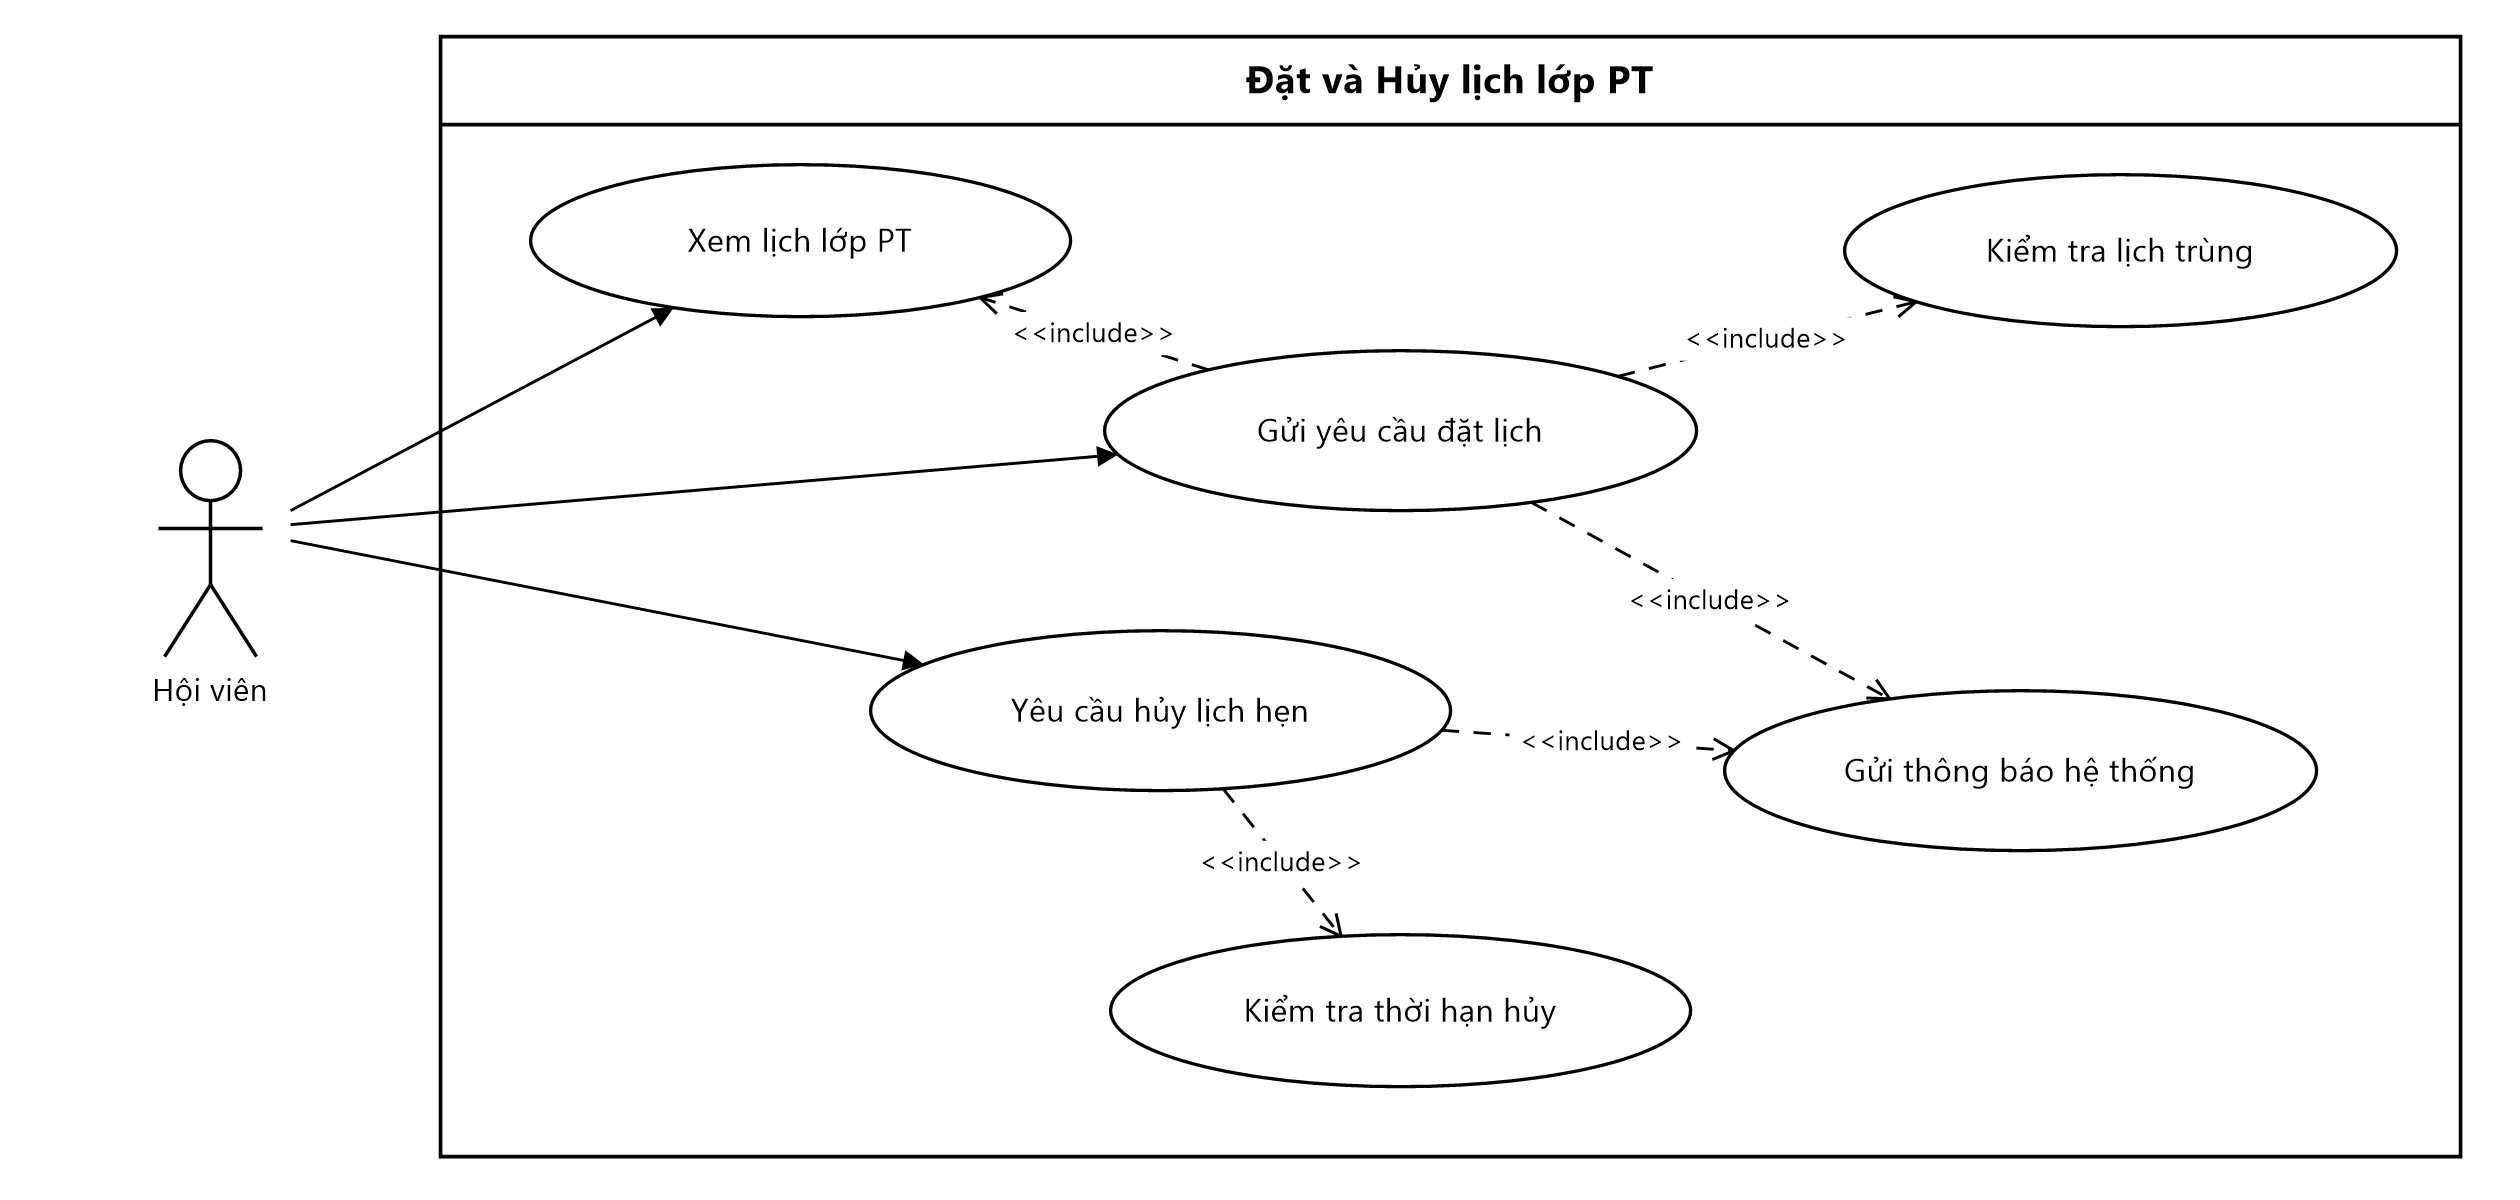
\includegraphics[width=0.88\textwidth, height=0.65\textheight, keepaspectratio]{images/uc_p21_1.png}
\caption{Use-case Đặt và Hủy lịch lớp PT}
\end{figure}

\begin{table}[H]\centering\footnotesize
\begin{tabularx}{\textwidth}{|L{3.2cm}|Y|}
\hline \textbf{Tóm tắt} & Hội viên đặt lịch tập 1-kèm-1 với PT theo khung giờ rảnh của PT; mỗi lần đặt thành công sẽ tạm trừ 1 buổi PT. \\ \hline
\textbf{Tiền điều kiện} & Hội viên đã đăng nhập; gói hội viên (có tặng kèm buổi PT) hoặc gói PT 1-kèm-1 còn hiệu lực và còn ít nhất 1 buổi. \\ \hline
\textbf{Dòng sự kiện chính} & 1. Hội viên xem lịch lớp PT để biết khung giờ trống của PT.\newline 2. Chọn khung giờ phù hợp và nhấn "Gửi yêu cầu đặt lịch".\newline 3. Hệ thống tạo yêu cầu trạng thái "Chờ duyệt" và tạm trừ 1 buổi PT (ưu tiên trừ buổi tặng kèm trước, sau đó mới trừ gói PT đã mua).\newline 4. Gửi thông báo hệ thống đến PT để chờ xác nhận. \\ \hline
\textbf{Dòng sự kiện phụ} & Nếu khung giờ chọn bị trùng với lịch lớp nhóm hoặc lịch hẹn khác của hội viên, hệ thống báo lỗi và yêu cầu chọn khung giờ khác. \\ \hline
\textbf{Hậu điều kiện} & Yêu cầu đặt lịch lưu trạng thái "Chờ duyệt", tạm trừ 1 buổi PT và PT nhận được thông báo. \\ \hline
\end{tabularx}
\caption{Bảng đặc tả Use-case 16: Gửi yêu cầu đặt lịch PT}
\end{table}

\begin{table}[H]\centering\footnotesize
\begin{tabularx}{\textwidth}{|L{3.2cm}|Y|}
\hline \textbf{Tóm tắt} & Hội viên thực hiện hủy một lịch hẹn tập với PT đã đặt trước đó. \\ \hline
\textbf{Tiền điều kiện} & Hội viên đã đăng nhập; tồn tại lịch hẹn ở trạng thái "Chờ duyệt" hoặc "Đã xác nhận". \\ \hline
\textbf{Dòng sự kiện chính} & 1. Hội viên vào danh sách lịch hẹn, chọn lịch PT (\texttt{Chờ duyệt} hoặc \texttt{Đã xác nhận} trước giờ tập) và nhấn "Hủy lịch hẹn".\newline 2. Hệ thống kiểm tra trạng thái và thời hạn hủy (trước giờ tập tối thiểu 8 tiếng đối với lịch đã xác nhận).\newline 3. Nếu hủy ở trạng thái \texttt{Chờ duyệt} hoặc hủy đúng hạn ($\ge 8$ giờ), hệ thống cập nhật trạng thái thành "Đã hủy" (\texttt{Cancelled}) và hoàn trả 1 buổi PT về nguồn đã trừ.\newline 4. Gửi thông báo cho PT và Hội viên biết lịch đã bị hủy. \\ \hline
\textbf{Dòng sự kiện phụ} & -- Hủy quá hạn (dưới 8 tiếng trước giờ tập đối với lịch đã xác nhận): hệ thống cảnh báo mất buổi PT; nếu hội viên vẫn xác nhận hủy, lịch chuyển sang trạng thái \texttt{Late\_Cancelled}, \textbf{không hoàn lại buổi PT} (tính đã sử dụng) và giải phóng khung giờ cho PT.\newline -- Nếu buổi tập đã diễn ra hoặc quá giờ bắt đầu: hệ thống không cho phép hủy. \\ \hline
\textbf{Hậu điều kiện} & Lịch hẹn chuyển sang trạng thái \texttt{Cancelled} hoặc \texttt{Late\_Cancelled}; số buổi PT được hoàn lại hoặc tính đã dùng đúng quy định. \\ \hline
\end{tabularx}
\caption{Bảng đặc tả Use-case 17: Yêu cầu hủy lịch hẹn PT}
\end{table}

\paragraph{13. Xác nhận yêu cầu và cập nhật lịch rảnh}
\begin{figure}[H]
\centering
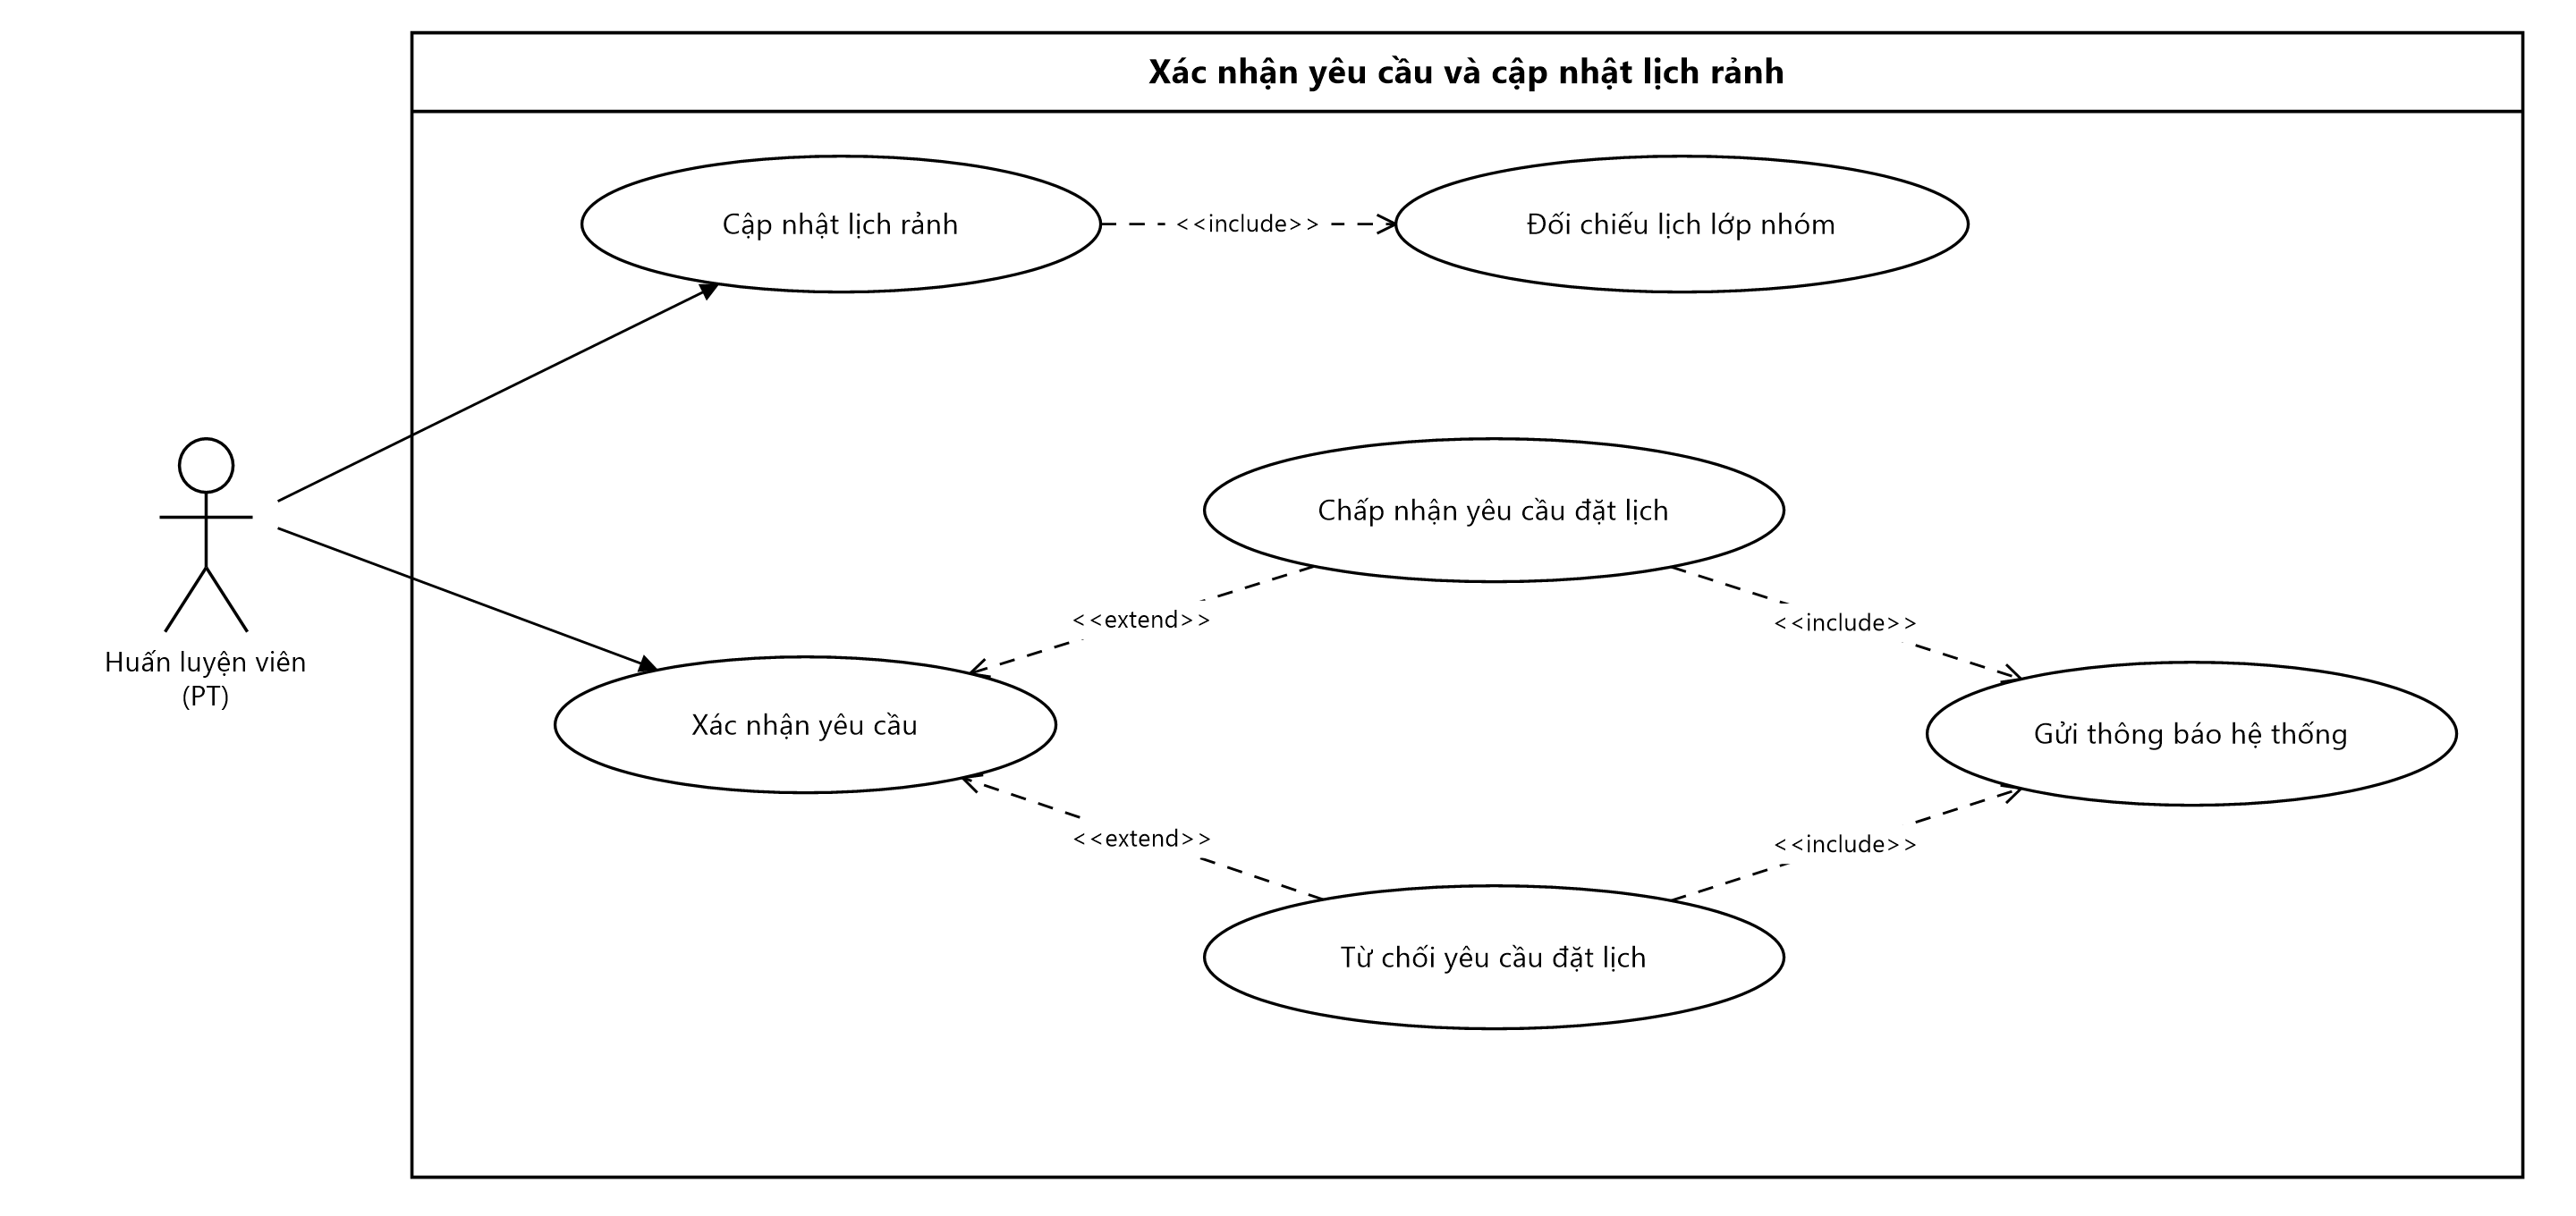
\includegraphics[width=0.88\textwidth, height=0.65\textheight, keepaspectratio]{images/uc_p23_1.png}
\caption{Use-case Xác nhận yêu cầu và cập nhật lịch rảnh}
\end{figure}

\begin{table}[H]\centering\footnotesize
\begin{tabularx}{\textwidth}{|L{3.2cm}|Y|}
\hline \textbf{Tóm tắt} & Huấn luyện viên (PT) thiết lập và cập nhật các khung giờ trống cá nhân trên hệ thống để hội viên xem và đặt lịch. \\ \hline
\textbf{Tiền điều kiện} & PT đã đăng nhập và hồ sơ chuyên môn đã được Admin duyệt. \\ \hline
\textbf{Dòng sự kiện chính} & 1. PT truy cập chức năng quản lý lịch làm việc.\newline 2. Chọn các ngày và khung giờ trống để mở ca nhận khách.\newline 3. Hệ thống tự động đối chiếu lịch lớp nhóm mà PT đang được phân công giảng dạy.\newline 4. Lưu các khung giờ rảnh hợp lệ và hiển thị lên danh sách cho hội viên. \\ \hline
\textbf{Dòng sự kiện phụ} & Nếu khung giờ rảnh trùng với thời gian dạy lớp học nhóm, hệ thống cảnh báo đỏ, không cho lưu và yêu cầu chỉnh sửa lại. \\ \hline
\textbf{Hậu điều kiện} & Lịch rảnh của Huấn luyện viên được cập nhật thành công lên hệ thống. \\ \hline
\end{tabularx}
\caption{Bảng đặc tả Use-case 18: Cập nhật lịch rảnh PT}
\end{table}

\begin{table}[H]\centering\footnotesize
\begin{tabularx}{\textwidth}{|L{3.2cm}|Y|}
\hline \textbf{Tóm tắt} & PT xem danh sách các yêu cầu đặt lịch do hội viên gửi tới và quyết định chấp nhận hoặc từ chối. \\ \hline
\textbf{Tiền điều kiện} & PT đã đăng nhập; tồn tại ít nhất một yêu cầu đặt lịch ở trạng thái "Chờ duyệt". \\ \hline
\textbf{Dòng sự kiện chính} & 1. PT mở danh sách thông báo/yêu cầu và chọn một yêu cầu đặt lịch.\newline 2. PT nhấn "Xác nhận yêu cầu".\newline 3. Hệ thống chuyển trạng thái lịch hẹn thành "Đã xác nhận".\newline 4. Gửi thông báo đến Hội viên báo lịch đã được duyệt. \\ \hline
\textbf{Dòng sự kiện phụ} & Nếu PT bận đột xuất và chọn "Từ chối", hệ thống chuyển trạng thái thành "Đã từ chối", hoàn trả lại 1 buổi PT cho hội viên và gửi thông báo. \\ \hline
\textbf{Hậu điều kiện} & Yêu cầu kết thúc ở trạng thái "Đã xác nhận" hoặc "Đã từ chối"; hội viên nhận được thông báo phản hồi. \\ \hline
\end{tabularx}
\caption{Bảng đặc tả Use-case 19: Xác nhận yêu cầu đặt lịch}
\end{table}

\paragraph{14. Check-in \& Check-out tại Chi nhánh}
\begin{figure}[H]
\centering
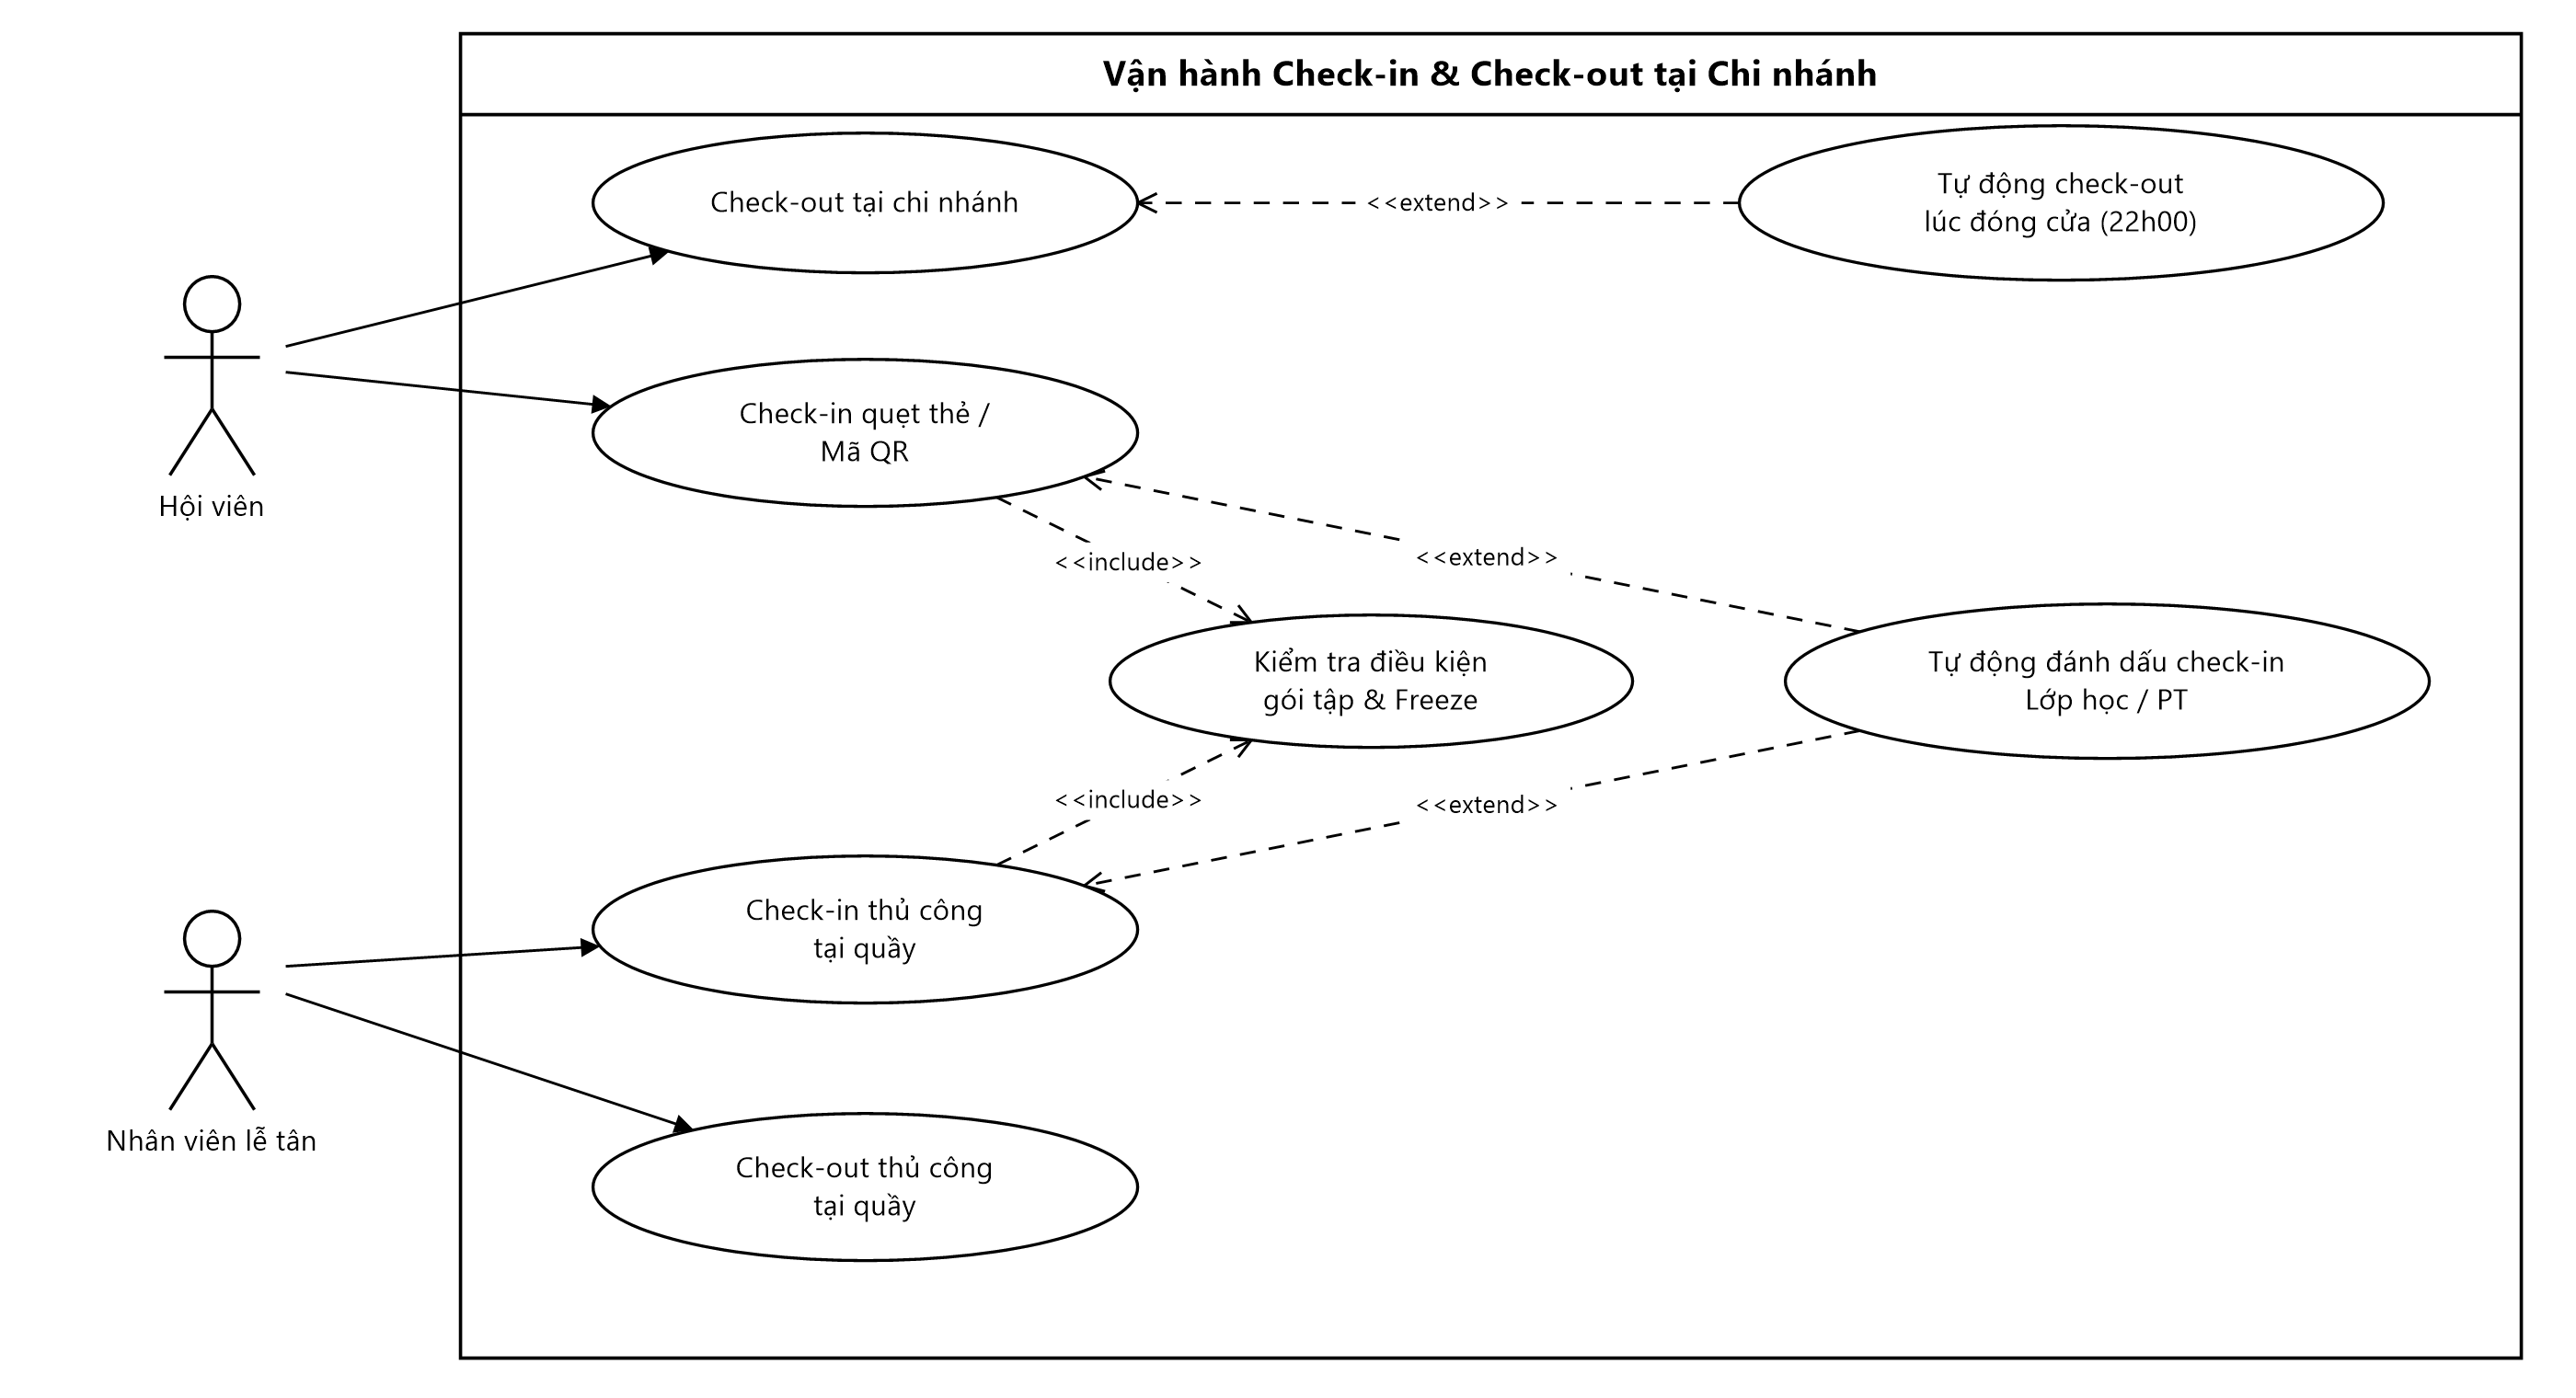
\includegraphics[width=0.88\textwidth, height=0.65\textheight, keepaspectratio]{images/uc_p25_1.png}
\caption{Use-case Check-in \& Check-out tại Chi nhánh}
\end{figure}

\begin{table}[H]\centering\footnotesize
\begin{tabularx}{\textwidth}{|L{3.2cm}|Y|}
\hline \textbf{Tóm tắt} & Hội viên quét thẻ thành viên (RFID hoặc mã QR) tại cổng tự động/Kiosk chi nhánh để xác thực thẻ, kiểm tra điều kiện gói tập và ghi nhận vào phòng tập. \\ \hline
\textbf{Tiền điều kiện} & Hội viên sở hữu thẻ \texttt{MemberCard} ở trạng thái \texttt{Active}; chưa có lượt check-in mở trong ngày. \\ \hline
\textbf{Dòng sự kiện chính} & 1. Hội viên đưa thẻ vật lý hoặc mã QR trên ứng dụng vào đầu đọc tại Kiosk chi nhánh.\newline 2. Hệ thống kiểm tra trạng thái thẻ \texttt{MemberCard} (\texttt{Active}) và tài khoản hội viên không bị khóa.\newline 3. Hệ thống gọi Use-case "Kiểm tra điều kiện gói tập \& Freeze" (bao gồm quyền tập chi nhánh).\newline 4. Nếu hợp lệ, hệ thống mở cổng/hiển thị kết quả thành công, ghi nhận nhật ký check-in và mở rộng sang "Tự động đánh dấu check-in Lớp học / PT". \\ \hline
\textbf{Dòng sự kiện phụ} & -- Thẻ ở trạng thái \texttt{Locked} hoặc \texttt{Lost}: từ chối quét, yêu cầu liên hệ lễ tân để hỗ trợ thủ công hoặc cấp lại thẻ mới.\newline -- Gói hết hạn / đang Freeze / sai chi nhánh / đang ở trong phòng tập chưa check-out: từ chối và hiển thị rõ lý do.\newline -- Lỗi thiết bị quét hoặc quên thẻ: chuyển sang Use-case "Check-in thủ công tại quầy". \\ \hline
\textbf{Hậu điều kiện} & Lượt check-in được ghi nhận vào nhật ký kèm thời gian vào và mã chi nhánh; các lịch lớp/PT trong ngày được gắn cờ đã check-in. \\ \hline
\end{tabularx}
\caption{Bảng đặc tả Use-case 20: Check-in quẹt thẻ / Mã QR}
\end{table}

\begin{table}[H]\centering\footnotesize
\begin{tabularx}{\textwidth}{|L{3.2cm}|Y|}
\hline \textbf{Tóm tắt} & Ghi nhận thời điểm hội viên rời khỏi phòng tập thông qua quét thẻ/QR tại Kiosk hoặc Lễ tân thao tác check-out thủ công tại quầy. \\ \hline
\textbf{Tiền điều kiện} & Hội viên đang có lượt check-in hợp lệ chưa đóng (\texttt{Check\_Out\_At = NULL}) trong ngày tại chi nhánh. \\ \hline
\textbf{Dòng sự kiện chính} & 1. Hội viên quét lại thẻ/QR tại Kiosk khi ra về hoặc báo Lễ tân chọn "Check-out" tại quầy.\newline 2. Hệ thống tìm lượt check-in đang mở trong ngày của hội viên.\newline 3. Hệ thống cập nhật thời gian ra (\texttt{Check\_Out\_At}), phương thức check-out và tính thời lượng buổi tập.\newline 4. Cập nhật giảm số lượng hội viên hiện diện tại chi nhánh. \\ \hline
\textbf{Dòng sự kiện phụ} & Nếu không tìm thấy lượt check-in mở trong ngày, hệ thống thông báo "Hội viên chưa check-in" và không ghi nhận check-out. \\ \hline
\textbf{Hậu điều kiện} & Lượt check-in được đóng lại an toàn kèm thời điểm rời phòng tập. \\ \hline
\end{tabularx}
\caption{Bảng đặc tả Use-case 21: Check-out tại chi nhánh}
\end{table}

\begin{table}[H]\centering\footnotesize
\begin{tabularx}{\textwidth}{|L{3.2cm}|Y|}
\hline \textbf{Tóm tắt} & Tác vụ tự động của hệ thống vào giờ đóng cửa chi nhánh (mặc định 22h00) nhằm đóng toàn bộ các lượt check-in còn mở do hội viên quên check-out. \\ \hline
\textbf{Tiền điều kiện} & Đến giờ đóng cửa chi nhánh (\texttt{Close\_Time}) và tồn tại lượt check-in trong ngày có \texttt{Check\_Out\_At = NULL}. \\ \hline
\textbf{Dòng sự kiện chính} & 1. Bộ lập lịch tự động quét danh sách lượt check-in thành công chưa có giờ check-out khi qua mốc đóng cửa.\newline 2. Với mỗi bản ghi tìm thấy, hệ thống gán \texttt{Check\_Out\_At} bằng giờ đóng cửa chi nhánh và đánh dấu \texttt{Is\_Auto\_Checkout = 1}.\newline 3. Lưu cập nhật nhật ký ra/vào của chi nhánh trong ngày. \\ \hline
\textbf{Dòng sự kiện phụ} & Không có lượt check-in nào còn mở $\rightarrow$ kết thúc chu kỳ quét an toàn. \\ \hline
\textbf{Hậu điều kiện} & Mọi lượt check-in trong ngày đều được đóng lại trước ngày vận hành mới. \\ \hline
\end{tabularx}
\caption{Bảng đặc tả Use-case 22: Tự động check-out lúc đóng cửa (22h00)}
\end{table}

\begin{table}[H]\centering\footnotesize
\begin{tabularx}{\textwidth}{|L{3.2cm}|Y|}
\hline \textbf{Tóm tắt} & Lễ tân tra cứu thông tin và đối chiếu khuôn mặt để thực hiện check-in cho hội viên khi quên thẻ, thẻ hỏng hoặc thiết bị quét lỗi. \\ \hline
\textbf{Tiền điều kiện} & Lễ tân đã đăng nhập hệ thống; hội viên có mặt tại quầy lễ tân chi nhánh. \\ \hline
\textbf{Dòng sự kiện chính} & 1. Lễ tân nhập SĐT hoặc họ tên hội viên vào ô tìm kiếm.\newline 2. Hệ thống hiển thị hồ sơ cá nhân và ảnh đại diện (avatar).\newline 3. Lễ tân đối chiếu khuôn mặt thực tế, chọn "Xác nhận Check-in thủ công" và nhập lý do.\newline 4. Hệ thống gọi Use-case "Kiểm tra điều kiện gói tập \& Freeze"; nếu hợp lệ thì ghi nhận lượt check-in kèm mã nhân viên và lý do. \\ \hline
\textbf{Dòng sự kiện phụ} & Không tìm thấy thông tin hội viên $\rightarrow$ Hệ thống báo lỗi, yêu cầu kiểm tra lại SĐT đã đăng ký. \\ \hline
\textbf{Hậu điều kiện} & Nhật ký check-in thủ công được lưu lại thành công trong hệ thống. \\ \hline
\end{tabularx}
\caption{Bảng đặc tả Use-case 23: Check-in thủ công tại quầy}
\end{table}

\begin{table}[H]\centering\footnotesize
\begin{tabularx}{\textwidth}{|L{3.2cm}|Y|}
\hline \textbf{Tóm tắt} & Hệ thống tự động kiểm tra hiệu lực gói, phạm vi chi nhánh và trạng thái tạm ngưng (freeze) trước khi cho phép check-in. \\ \hline
\textbf{Tiền điều kiện} & Có yêu cầu check-in kích hoạt từ quét thẻ/QR hoặc check-in thủ công tại quầy. \\ \hline
\textbf{Dòng sự kiện chính} & 1. Kiểm tra thời hạn sử dụng của gói tập hội viên.\newline 2. Kiểm tra gói tập có đang nằm trong thời gian tạm ngưng (freeze) hay không.\newline 3. Đối chiếu quyền tập tại chi nhánh hiện tại theo cấu hình gói.\newline 4. Nếu hợp lệ, trả về kết quả "Hợp lệ". \\ \hline
\textbf{Dòng sự kiện phụ} & -- Gói hết hạn: từ chối, cảnh báo hết hạn và nhắc gia hạn.\newline -- Gói đang Freeze: từ chối, thông báo gói đang tạm ngưng.\newline -- Sai chi nhánh: từ chối, thông báo gói không hỗ trợ tập chéo tại chi nhánh này. \\ \hline
\textbf{Hậu điều kiện} & Kết quả kiểm tra (Hợp lệ / Từ chối kèm lý do) được trả về cho Use-case check-in. \\ \hline
\end{tabularx}
\caption{Bảng đặc tả Use-case 24: Kiểm tra điều kiện gói tập \& Freeze}
\end{table}

\begin{table}[H]\centering\footnotesize
\begin{tabularx}{\textwidth}{|L{3.2cm}|Y|}
\hline \textbf{Tóm tắt} & Khi check-in vào chi nhánh thành công, hệ thống tự động nhận diện các lịch học lớp nhóm hoặc lịch hẹn PT trong ngày tại chi nhánh đó để gắn cờ đã check-in. \\ \hline
\textbf{Tiền điều kiện} & Hội viên vừa check-in vào chi nhánh thành công và có lịch đặt lớp nhóm (\texttt{Booked}) hoặc lịch PT (\texttt{Confirmed}) trong ngày tại cùng chi nhánh. \\ \hline
\textbf{Dòng sự kiện chính} & 1. Quét danh sách lịch lớp nhóm và lịch hẹn PT của hội viên trong ngày tại chi nhánh vừa check-in.\newline 2. Gắn cờ trạng thái đã check-in (\texttt{CheckedIn = true}) cho các buổi tập tương ứng.\newline 3. Cung cấp cờ dữ liệu này lên màn hình điểm danh của HLV để xác nhận tham gia thực tế. \\ \hline
\textbf{Dòng sự kiện phụ} & Nếu không có lịch lớp/PT trong ngày tại chi nhánh, hệ thống bỏ qua bước gắn cờ và chỉ ghi nhận lượt tập tự do. \\ \hline
\textbf{Hậu điều kiện} & Cờ đã check-in được cập nhật làm điều kiện bắt buộc để HLV xác nhận có mặt (\texttt{Attended}/\texttt{Completed}) sau buổi tập. \\ \hline
\end{tabularx}
\caption{Bảng đặc tả Use-case 25: Tự động đánh dấu check-in lớp học / PT}
\end{table}

\paragraph{15. Chi nhánh \& Thiết bị}
\begin{figure}[H]
\centering
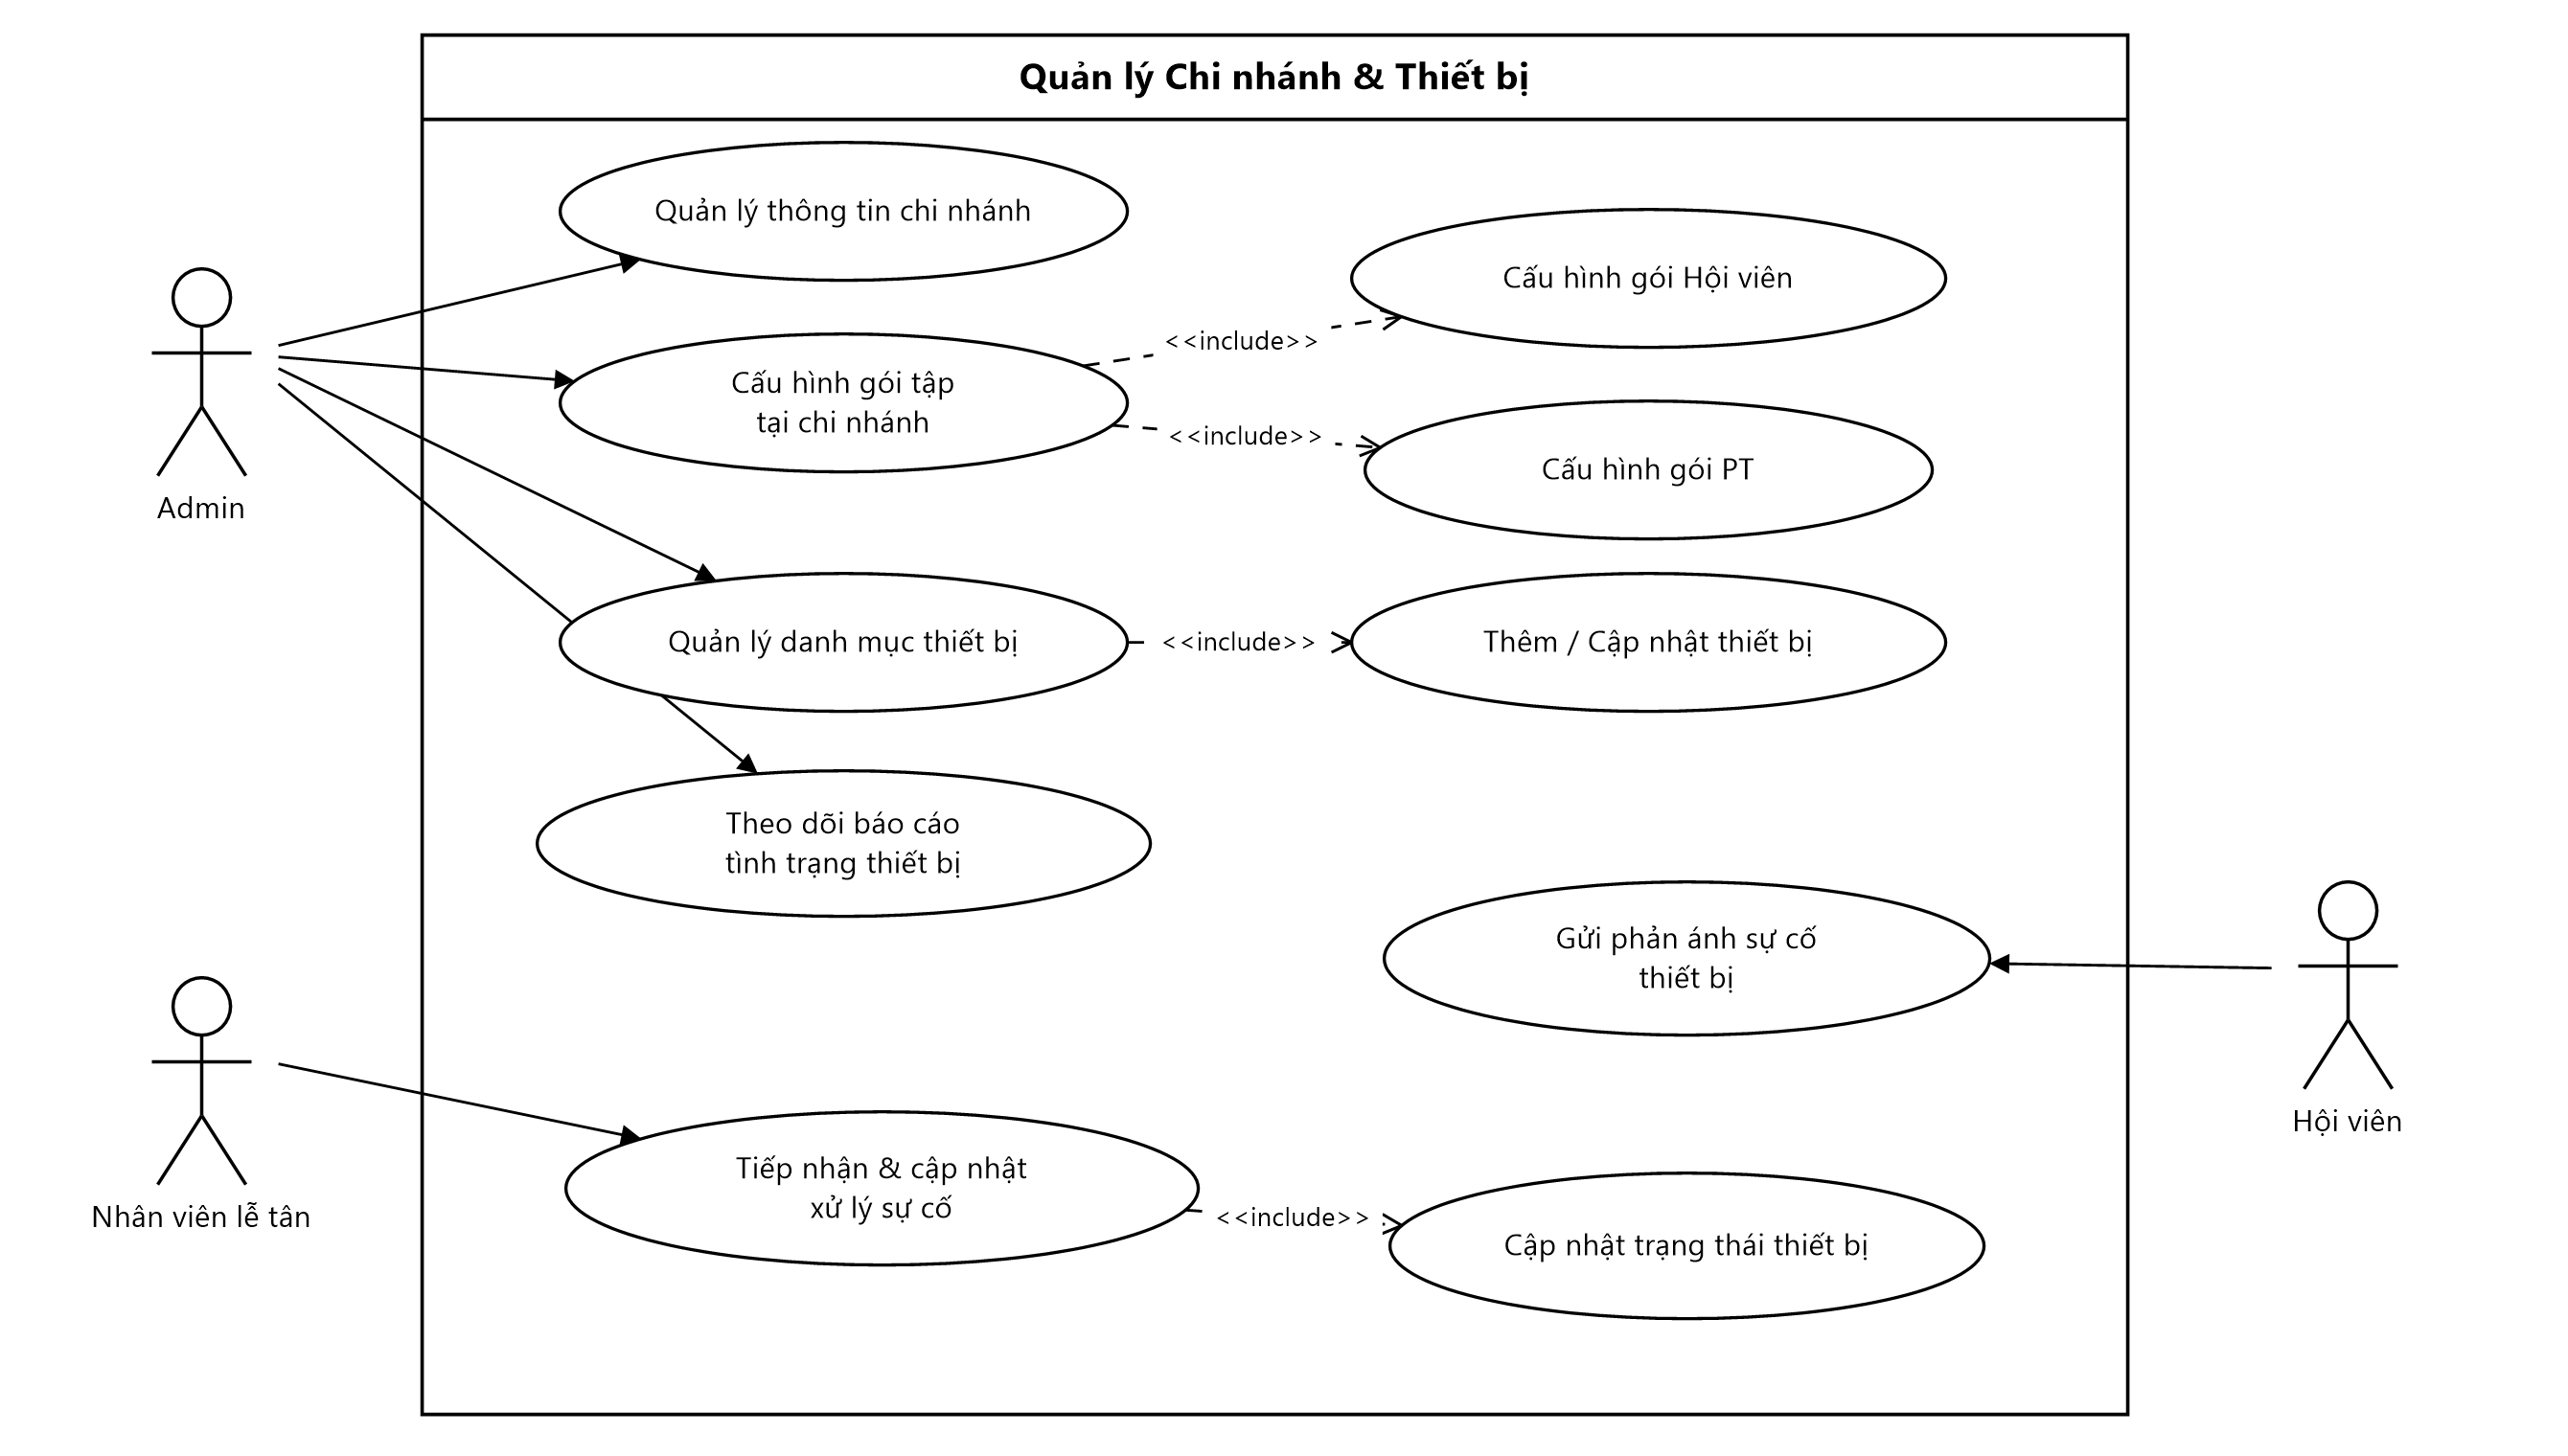
\includegraphics[width=0.88\textwidth, height=0.65\textheight, keepaspectratio]{images/uc_p27_1.png}
\caption{Use-case Chi nhánh \& Thiết bị}
\end{figure}

\begin{table}[H]\centering\footnotesize
\begin{tabularx}{\textwidth}{|L{3.2cm}|Y|}
\hline \textbf{Tóm tắt} & Admin khai báo chi nhánh mới (tên, địa chỉ, thông tin liên hệ) và thiết lập các gói tập được phép áp dụng tại từng chi nhánh. \\ \hline
\textbf{Tiền điều kiện} & Admin đã đăng nhập hệ thống với quyền quản trị. \\ \hline
\textbf{Dòng sự kiện chính} & 1. Admin chọn "Quản lý chi nhánh" $\rightarrow$ "Thêm chi nhánh mới".\newline 2. Nhập thông tin (tên, địa chỉ, SĐT...), hệ thống kiểm tra hợp lệ.\newline 3. Admin chọn các gói tập áp dụng cho chi nhánh.\newline 4. Hệ thống lưu thông tin chi nhánh và cấu hình gói tập. \\ \hline
\textbf{Dòng sự kiện phụ} & Thông tin không hợp lệ (trùng tên, thiếu trường bắt buộc) $\rightarrow$ báo lỗi yêu cầu nhập lại; hỗ trợ chỉnh sửa/xóa chi nhánh hiện có. \\ \hline
\textbf{Hậu điều kiện} & Chi nhánh cùng cấu hình gói tập áp dụng được lưu vào hệ thống. \\ \hline
\end{tabularx}
\caption{Bảng đặc tả Use-case 26: Quản lý thông tin chi nhánh \& Cấu hình gói tập}
\end{table}

\begin{table}[H]\centering\footnotesize
\begin{tabularx}{\textwidth}{|L{3.2cm}|Y|}
\hline \textbf{Tóm tắt} & Tác vụ kiểm tra hệ thống (được gọi trong quy trình check-in ở Nhóm 14) nhằm xác định gói tập của hội viên có áp dụng tại chi nhánh hiện tại hay không (\texttt{Is\_All\_Branches} hoặc \texttt{Plan\_Branches}). \\ \hline
\textbf{Tiền điều kiện} & Phát sinh yêu cầu check-in tại một chi nhánh; hội viên có gói tập \texttt{Active}. \\ \hline
\textbf{Dòng sự kiện chính} & 1. Tiếp nhận mã hội viên và mã chi nhánh từ yêu cầu check-in.\newline 2. Hệ thống truy vấn gói tập hiện tại và danh sách chi nhánh được áp dụng của gói.\newline 3. Đối chiếu chi nhánh hiện tại với cấu hình phạm vi chi nhánh (\texttt{Is\_All\_Branches = 1} hoặc tồn tại trong \texttt{Plan\_Branches}).\newline 4. Trả về kết quả hợp lệ/từ chối cho luồng check-in. \\ \hline
\textbf{Dòng sự kiện phụ} & Gói không cho tập chéo hoặc đã hết hạn $\rightarrow$ từ chối check-in và thông báo lý do. \\ \hline
\textbf{Hậu điều kiện} & Quyền truy cập chi nhánh được xác định (cho phép/từ chối) và ghi nhận vào lịch sử. \\ \hline
\end{tabularx}
\caption{Bảng đặc tả Use-case 27: Kiểm tra quyền tập chéo chi nhánh}
\end{table}

\begin{table}[H]\centering\footnotesize
\begin{tabularx}{\textwidth}{|L{3.2cm}|Y|}
\hline \textbf{Tóm tắt} & Admin thêm mới, cập nhật hoặc xóa thông tin máy tập tại từng chi nhánh. \\ \hline
\textbf{Tiền điều kiện} & Admin đã đăng nhập; chi nhánh cần quản lý thiết bị đã tồn tại. \\ \hline
\textbf{Dòng sự kiện chính} & 1. Admin chọn "Quản lý thiết bị", hệ thống hiển thị danh sách thiết bị theo chi nhánh.\newline 2. Chọn "Thêm thiết bị mới", nhập thông tin (tên, loại, chi nhánh, ngày nhập...).\newline 3. Hệ thống kiểm tra hợp lệ và lưu thiết bị mới. \\ \hline
\textbf{Dòng sự kiện phụ} & Admin có thể sửa/xóa thiết bị hiện có; nếu thông tin không hợp lệ thì báo lỗi yêu cầu nhập lại. \\ \hline
\textbf{Hậu điều kiện} & Danh mục thiết bị của chi nhánh được cập nhật, phản ánh đúng tình trạng hiện tại. \\ \hline
\end{tabularx}
\caption{Bảng đặc tả Use-case 28: Quản lý danh mục thiết bị}
\end{table}

\begin{table}[H]\centering\footnotesize
\begin{tabularx}{\textwidth}{|L{3.2cm}|Y|}
\hline \textbf{Tóm tắt} & Admin xem báo cáo tổng hợp số lượng thiết bị đang hoạt động/đang sửa chữa/ngừng hoạt động trên toàn hệ thống. \\ \hline
\textbf{Tiền điều kiện} & Admin đã đăng nhập; có dữ liệu thiết bị và lịch sử xử lý sự cố. \\ \hline
\textbf{Dòng sự kiện chính} & 1. Admin chọn "Báo cáo tình trạng thiết bị".\newline 2. Hệ thống tổng hợp số liệu theo trạng thái và theo chi nhánh, hiển thị dạng bảng/biểu đồ.\newline 3. Admin lọc theo chi nhánh/thời gian và xuất báo cáo (Excel/PDF) nếu cần. \\ \hline
\textbf{Dòng sự kiện phụ} & Không có dữ liệu khớp bộ lọc $\rightarrow$ thông báo "Không có dữ liệu"; lỗi xuất báo cáo $\rightarrow$ thông báo cho thử lại. \\ \hline
\textbf{Hậu điều kiện} & Admin có cái nhìn tổng quan về tình trạng thiết bị toàn hệ thống để ra quyết định bảo trì/thay thế. \\ \hline
\end{tabularx}
\caption{Bảng đặc tả Use-case 29: Theo dõi báo cáo tình trạng thiết bị}
\end{table}

\begin{table}[H]\centering\footnotesize
\begin{tabularx}{\textwidth}{|L{3.2cm}|Y|}
\hline \textbf{Tóm tắt} & Hội viên phát hiện máy tập bị hỏng, chụp ảnh và gửi báo cáo sự cố qua ứng dụng. \\ \hline
\textbf{Tiền điều kiện} & Hội viên đã đăng nhập; đang ở chi nhánh có thiết bị hỏng. \\ \hline
\textbf{Dòng sự kiện chính} & 1. Hội viên chọn chức năng "Báo sự cố thiết bị".\newline 2. Chọn thiết bị bị hỏng tại chi nhánh hiện tại, chụp ảnh và mô tả sự cố.\newline 3. Gửi phản ánh; hệ thống ghi nhận trạng thái "Chờ xử lý", chuyển đến lễ tân chi nhánh và thông báo thành công. \\ \hline
\textbf{Dòng sự kiện phụ} & Không đính kèm ảnh $\rightarrow$ vẫn cho gửi kèm cảnh báo; mất kết nối $\rightarrow$ lưu nháp cho phép gửi lại sau. \\ \hline
\textbf{Hậu điều kiện} & Phản ánh sự cố được ghi nhận trạng thái chờ xử lý, chuyển đến nhân viên lễ tân phụ trách. \\ \hline
\end{tabularx}
\caption{Bảng đặc tả Use-case 30: Gửi phản ánh sự cố thiết bị}
\end{table}

\begin{table}[H]\centering\footnotesize
\begin{tabularx}{\textwidth}{|L{3.2cm}|Y|}
\hline \textbf{Tóm tắt} & Lễ tân tiếp nhận các phản ánh sự cố thiết bị, ghi nhận tình trạng và cập nhật khi thiết bị đã được sửa xong. \\ \hline
\textbf{Tiền điều kiện} & Có phản ánh sự cố ở trạng thái "Chờ xử lý"; lễ tân đã đăng nhập. \\ \hline
\textbf{Dòng sự kiện chính} & 1. Lễ tân mở danh sách phản ánh sự cố và xem chi tiết (ảnh, mô tả).\newline 2. Cập nhật trạng thái thành "Đang sửa chữa" kèm ghi chú.\newline 3. Khi sửa xong, cập nhật trạng thái thành "Đã sửa xong/Hoạt động"; hệ thống cập nhật trạng thái thiết bị. \\ \hline
\textbf{Dòng sự kiện phụ} & Thiết bị hỏng nặng $\rightarrow$ đánh dấu "Ngừng hoạt động" và báo Admin; phản ánh trùng lặp/sai $\rightarrow$ đánh dấu "Đã hủy" kèm lý do. \\ \hline
\textbf{Hậu điều kiện} & Trạng thái sự cố và trạng thái hoạt động của thiết bị được cập nhật chính xác trong hệ thống. \\ \hline
\end{tabularx}
\caption{Bảng đặc tả Use-case 31: Tiếp nhận \& cập nhật xử lý sự cố thiết bị}
\end{table}

\paragraph{16. Theo dõi Tiến độ \& Đánh giá}
\begin{figure}[H]
\centering
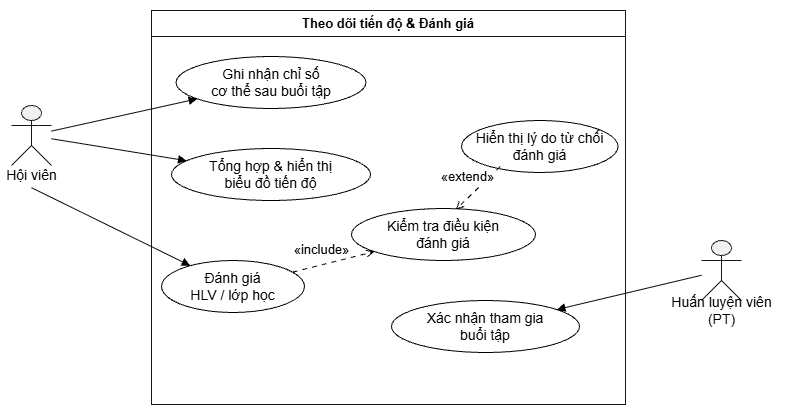
\includegraphics[width=0.88\textwidth, height=0.65\textheight, keepaspectratio]{images/uc_p31_1.png}
\caption{Use-case Theo dõi Tiến độ \& Đánh giá}
\end{figure}

\begin{table}[H]\centering\footnotesize
\begin{tabularx}{\textwidth}{|L{3.2cm}|Y|}
\hline \textbf{Tóm tắt} & Hội viên nhập các chỉ số cơ thể (cân nặng, chiều cao, BMI, tỷ lệ mỡ, khối lượng cơ) sau buổi tập để hệ thống lưu vào lịch sử đo. \\ \hline
\textbf{Tiền điều kiện} & Hội viên đã đăng nhập, có hồ sơ cá nhân và vừa kết thúc buổi tập. \\ \hline
\textbf{Dòng sự kiện chính} & 1. Hội viên chọn chức năng cập nhật chỉ số cơ thể.\newline 2. Hệ thống hiển thị Phiếu chỉ số mới và Lịch sử chỉ số cơ thể.\newline 3. Hội viên nhập các chỉ số đo được và bấm lưu.\newline 4. Hệ thống kiểm tra hợp lệ, ghi nhận kèm thời điểm đo và lưu vào lịch sử đo. \\ \hline
\textbf{Dòng sự kiện phụ} & Chỉ số không hợp lệ $\rightarrow$ từ chối lưu và yêu cầu nhập lại. Nếu chưa có mốc ban đầu $\rightarrow$ lần đo này lưu làm mốc ban đầu; các lần sau lưu thành lịch sử và không ghi đè mốc. \\ \hline
\textbf{Hậu điều kiện} & Lần đo mới được lưu vào Lịch sử chỉ số cơ thể kèm thời điểm đo; mốc ban đầu không bị thay đổi. \\ \hline
\end{tabularx}
\caption{Bảng đặc tả Use-case 32: Ghi nhận chỉ số cơ thể sau buổi tập}
\end{table}

\begin{table}[H]\centering\footnotesize
\begin{tabularx}{\textwidth}{|L{3.2cm}|Y|}
\hline \textbf{Tóm tắt} & Hệ thống tổng hợp lịch sử đo của hội viên và vẽ biểu đồ đường thể hiện sự thay đổi của từng chỉ số so với mốc ban đầu. \\ \hline
\textbf{Tiền điều kiện} & Hội viên đã đăng nhập, yêu cầu xem tiến độ và đã có ít nhất một lần đo trong lịch sử. \\ \hline
\textbf{Dòng sự kiện chính} & 1. Hội viên chọn xem biểu đồ tiến độ và chọn chỉ số muốn theo dõi.\newline 2. Hệ thống lấy Lịch sử chỉ số cơ thể của chính hội viên, sắp xếp theo thời gian.\newline 3. Lấy mốc ban đầu làm điểm so sánh, tổng hợp và hiển thị biểu đồ đường. \\ \hline
\textbf{Dòng sự kiện phụ} & Mới chỉ có mốc ban đầu $\rightarrow$ chỉ hiển thị mốc ban đầu và thông báo cần thêm lần đo để thấy sự thay đổi. \\ \hline
\textbf{Hậu điều kiện} & Biểu đồ tiến độ được hiển thị; dữ liệu lịch sử đo không bị thay đổi. \\ \hline
\end{tabularx}
\caption{Bảng đặc tả Use-case 33: Tổng hợp \& hiển thị biểu đồ tiến độ}
\end{table}

\begin{table}[H]\centering\footnotesize
\begin{tabularx}{\textwidth}{|L{3.2cm}|Y|}
\hline \textbf{Tóm tắt} & PT đối chiếu cờ đã check-in hợp lệ tại chi nhánh trong ngày để xác nhận hội viên thực sự tham gia buổi tập (lớp nhóm hoặc PT 1-kèm-1) và mở quyền đánh giá. \\ \hline
\textbf{Tiền điều kiện} & Buổi tập đã kết thúc và PT là người phụ trách buổi tập đó. \\ \hline
\textbf{Dòng sự kiện chính} & 1. PT chọn buổi tập vừa kết thúc và xem danh sách hội viên.\newline 2. Hệ thống hiển thị Danh sách check-in để PT đối chiếu.\newline 3. PT bấm xác nhận tham gia cho từng hội viên đã thực tập.\newline 4. Hệ thống ghi nhận kết quả tham gia và mở quyền đánh giá cho hội viên. \\ \hline
\textbf{Dòng sự kiện phụ} & Hội viên không có check-in hợp lệ hoặc vắng mặt $\rightarrow$ không cho xác nhận tham gia và không mở quyền đánh giá. \\ \hline
\textbf{Hậu điều kiện} & Kết quả tham gia được ghi nhận và hội viên được mở quyền đánh giá buổi tập tương ứng. \\ \hline
\end{tabularx}
\caption{Bảng đặc tả Use-case 34: Xác nhận tham gia buổi tập}
\end{table}

\begin{table}[H]\centering\footnotesize
\begin{tabularx}{\textwidth}{|L{3.2cm}|Y|}
\hline \textbf{Tóm tắt} & Hội viên chấm điểm và nhận xét về HLV hoặc lớp học sau khi đã được xác nhận tham gia buổi tương ứng. \\ \hline
\textbf{Tiền điều kiện} & Hội viên đã đăng nhập và đã được xác nhận tham gia buổi tập cần đánh giá. \\ \hline
\textbf{Dòng sự kiện chính} & 1. Hội viên chọn buổi tập đã tham gia và đối tượng cần đánh giá (HLV hoặc lớp học).\newline 2. Hệ thống gọi Use-case "Kiểm tra điều kiện đánh giá".\newline 3. Nếu hợp lệ, hiển thị biểu mẫu; hội viên nhập điểm sao và nhận xét rồi bấm gửi.\newline 4. Lưu Phiếu đánh giá gắn với buổi tập, hội viên và đối tượng vào Lịch sử đánh giá. \\ \hline
\textbf{Dòng sự kiện phụ} & Điểm ngoài thang quy định $\rightarrow$ yêu cầu nhập lại. Kết quả kiểm tra từ chối $\rightarrow$ hiển thị lý do từ chối đánh giá. \\ \hline
\textbf{Hậu điều kiện} & Phiếu đánh giá được ghi nhận; buổi tập đó không thể đánh giá lại; làm đầu vào cho Báo cáo \& Thống kê. \\ \hline
\end{tabularx}
\caption{Bảng đặc tả Use-case 35: Đánh giá HLV / lớp học}
\end{table}

\begin{table}[H]\centering\footnotesize
\begin{tabularx}{\textwidth}{|L{3.2cm}|Y|}
\hline \textbf{Tóm tắt} & Hệ thống tự động kiểm tra buổi tập mà hội viên chọn đã được xác nhận tham gia và chưa được đánh giá, rồi cho phép hoặc từ chối. \\ \hline
\textbf{Tiền điều kiện} & Hội viên chọn đánh giá một buổi tập (Use-case "Đánh giá HLV / lớp học" được kích hoạt). \\ \hline
\textbf{Dòng sự kiện chính} & 1. Tiếp nhận thông tin buổi tập và hội viên cần đánh giá.\newline 2. Đối chiếu Danh sách xác nhận tham gia để kiểm tra hội viên đã tham gia buổi đó.\newline 3. Đối chiếu Lịch sử đánh giá để kiểm tra buổi đó chưa được hội viên đánh giá.\newline 4. Nếu đủ điều kiện, trả về kết quả "cho phép". \\ \hline
\textbf{Dòng sự kiện phụ} & Chưa xác nhận tham gia hoặc đã đánh giá $\rightarrow$ ghi kết quả "từ chối" kèm lý do và mở rộng sang Use-case "Hiển thị lý do từ chối đánh giá". \\ \hline
\textbf{Hậu điều kiện} & Kết quả kiểm tra điều kiện (cho phép hoặc từ chối kèm lý do) được ghi nhận để tiếp tục hoặc dừng lại. \\ \hline
\end{tabularx}
\caption{Bảng đặc tả Use-case 36: Kiểm tra điều kiện đánh giá}
\end{table}

\begin{table}[H]\centering\footnotesize
\begin{tabularx}{\textwidth}{|L{3.2cm}|Y|}
\hline \textbf{Tóm tắt} & Khi kết quả kiểm tra điều kiện là từ chối, hệ thống thông báo lý do (chưa tham gia / đã đánh giá) cho hội viên và dừng quy trình. \\ \hline
\textbf{Tiền điều kiện} & Use-case "Kiểm tra điều kiện đánh giá" ghi kết quả "từ chối" kèm lý do. \\ \hline
\textbf{Dòng sự kiện chính} & 1. Nhận kết quả từ chối kèm lý do.\newline 2. Hiển thị lý do từ chối (chưa tham gia / đã đánh giá) cho hội viên.\newline 3. Không hiển thị biểu mẫu đánh giá và kết thúc quy trình. \\ \hline
\textbf{Dòng sự kiện phụ} & Không có. \\ \hline
\textbf{Hậu điều kiện} & Hội viên biết lý do không được đánh giá; không có Phiếu đánh giá nào được tạo. \\ \hline
\end{tabularx}
\caption{Bảng đặc tả Use-case 37: Hiển thị lý do từ chối đánh giá}
\end{table}

\paragraph{17. Báo cáo \& Thống kê}
\begin{figure}[H]
\centering
\includegraphics[page=35, width=0.88\textwidth, trim=2.2cm 4.2cm 2.2cm 12.2cm, clip]{UC-Sequence_NhomBaKhi.pdf}
\caption{Use-case Báo cáo \& Thống kê}
\end{figure}

\begin{table}[H]\centering\footnotesize
\begin{tabularx}{\textwidth}{|L{3.2cm}|Y|}
\hline \textbf{Tóm tắt} & Hệ thống tổng hợp các nguồn thu tài chính từ gói hội viên, gói PT cá nhân và các dịch vụ khác theo kỳ hoặc theo từng chi nhánh. \\ \hline
\textbf{Tiền điều kiện} & Quản trị viên (Admin) đã đăng nhập với quyền quản trị tài chính. \\ \hline
\textbf{Dòng sự kiện chính} & 1. Admin chọn "Thống kê doanh thu", chọn khoảng thời gian và phạm vi chi nhánh.\newline 2. Hệ thống truy vấn lịch sử giao dịch thanh toán thành công.\newline 3. Phân loại doanh thu (gói hội viên, gói PT 1-kèm-1, nguồn thu bổ sung).\newline 4. Hiển thị biểu đồ tăng trưởng doanh thu và bảng số liệu chi tiết. \\ \hline
\textbf{Dòng sự kiện phụ} & Khoảng thời gian hoặc chi nhánh không phát sinh giao dịch $\rightarrow$ hiển thị mức doanh thu bằng 0. \\ \hline
\textbf{Hậu điều kiện} & Báo cáo chi tiết số liệu doanh thu được hiển thị đầy đủ cho Admin. \\ \hline
\end{tabularx}
\caption{Bảng đặc tả Use-case 38: Thống kê doanh thu}
\end{table}

\begin{table}[H]\centering\footnotesize
\begin{tabularx}{\textwidth}{|L{3.2cm}|Y|}
\hline \textbf{Tóm tắt} & Hệ thống tính toán lượng hội viên mới đăng ký, hội viên đang hoạt động (active) và tỷ lệ rời bỏ (churn rate). \\ \hline
\textbf{Tiền điều kiện} & Admin đăng nhập thành công và truy cập phân hệ thống kê hội viên. \\ \hline
\textbf{Dòng sự kiện chính} & 1. Admin chọn "Thống kê hội viên \& Churn rate", thiết lập bộ lọc chi nhánh và thời gian.\newline 2. Hệ thống tổng hợp số tài khoản mới, số gói còn hiệu lực và số gói hết hạn không gia hạn.\newline 3. Tính tỷ lệ rời bỏ ($\text{Churn rate} = \text{Số hội viên rời đi} / \text{Tổng số hội viên ban đầu}$) và vẽ biểu đồ.\newline 4. Hiển thị danh sách phân loại hội viên (mới, trung thành, có nguy cơ rời bỏ). \\ \hline
\textbf{Dòng sự kiện phụ} & Không có biến động hội viên trong kỳ $\rightarrow$ hiển thị thông báo trạng thái hội viên ổn định. \\ \hline
\textbf{Hậu điều kiện} & Biểu đồ xu hướng biến động và tỷ lệ giữ chân/rời bỏ của hội viên được hiển thị trực quan. \\ \hline
\end{tabularx}
\caption{Bảng đặc tả Use-case 39: Thống kê hội viên \& Churn rate}
\end{table}

\begin{table}[H]\centering\footnotesize
\begin{tabularx}{\textwidth}{|L{3.2cm}|Y|}
\hline \textbf{Tóm tắt} & Theo dõi số lượng gói hội viên đang hiệu lực/hết hạn, số gói đang tạm ngưng (freeze) và số buổi PT đã tiêu thụ/còn tồn. \\ \hline
\textbf{Tiền điều kiện} & Admin truy cập mục theo dõi tình trạng gói dịch vụ và lượt tập. \\ \hline
\textbf{Dòng sự kiện chính} & 1. Admin chọn "Thống kê sử dụng gói tập \& lượt PT".\newline 2. Hệ thống truy vấn số gói active, số gói freeze, số buổi PT đã hoàn thành và còn tồn.\newline 3. Hiển thị bảng phân tích chi tiết theo từng loại gói tập và chi nhánh. \\ \hline
\textbf{Dòng sự kiện phụ} & Admin lọc theo một chi nhánh duy nhất $\rightarrow$ hệ thống lọc chính xác dữ liệu của chi nhánh đó. \\ \hline
\textbf{Hậu điều kiện} & Báo cáo hiện trạng sử dụng tài nguyên gói tập và buổi PT được cung cấp cho Admin. \\ \hline
\end{tabularx}
\caption{Bảng đặc tả Use-case 40: Thống kê tình trạng sử dụng gói tập \& lượt PT}
\end{table}

\begin{table}[H]\centering\footnotesize
\begin{tabularx}{\textwidth}{|L{3.2cm}|Y|}
\hline \textbf{Tóm tắt} & Thống kê tỷ lệ lấp đầy chỗ (fill rate) và tỷ lệ tham gia thực tế (attendance rate) của các lớp học nhóm tại từng cơ sở. \\ \hline
\textbf{Tiền điều kiện} & Có dữ liệu các lớp học nhóm đã được tổ chức và lưu trữ trên hệ thống. \\ \hline
\textbf{Dòng sự kiện chính} & 1. Admin chọn "Thống kê hiệu suất lớp học", chọn cơ sở và khoảng thời gian.\newline 2. Tổng hợp số lượt đặt chỗ, số người trong Waitlist và số hội viên đã điểm danh trên sĩ số tối đa.\newline 3. Tính tỷ lệ lấp đầy, tỷ lệ vắng mặt và hiển thị bảng xếp hạng lớp học. \\ \hline
\textbf{Dòng sự kiện phụ} & Buổi học bị hủy trước giờ bắt đầu $\rightarrow$ không đưa vào tính tỷ lệ điểm danh thực tế. \\ \hline
\textbf{Hậu điều kiện} & Báo cáo hiệu suất vận hành và khai thác các lớp học nhóm được hiển thị cho Admin. \\ \hline
\end{tabularx}
\caption{Bảng đặc tả Use-case 41: Thống kê hiệu suất lớp học}
\end{table}

\begin{table}[H]\centering\footnotesize
\begin{tabularx}{\textwidth}{|L{3.2cm}|Y|}
\hline \textbf{Tóm tắt} & Thống kê tổng số buổi dạy, số hội viên phục vụ và điểm đánh giá sao trung bình của từng huấn luyện viên (PT). \\ \hline
\textbf{Tiền điều kiện} & Admin truy cập vào mục quản lý nhân sự và chất lượng dịch vụ. \\ \hline
\textbf{Dòng sự kiện chính} & 1. Admin chọn "Thống kê hiệu suất Huấn luyện viên".\newline 2. Tổng hợp số buổi 1-kèm-1 đã dạy và số lớp học nhóm đã đứng lớp của từng HLV.\newline 3. Tổng hợp điểm số từ phiếu đánh giá để tính điểm sao trung bình và hiển thị bảng xếp hạng HLV. \\ \hline
\textbf{Dòng sự kiện phụ} & HLV mới chưa có buổi dạy hoặc chưa nhận đánh giá $\rightarrow$ hiển thị "Chưa có dữ liệu đánh giá". \\ \hline
\textbf{Hậu điều kiện} & Dữ liệu hiệu suất làm việc và mức độ hài lòng của khách hàng đối với đội ngũ PT được hiển thị chi tiết. \\ \hline
\end{tabularx}
\caption{Bảng đặc tả Use-case 42: Thống kê hiệu suất HLV}
\end{table}

\begin{table}[H]\centering\footnotesize
\begin{tabularx}{\textwidth}{|L{3.2cm}|Y|}
\hline \textbf{Tóm tắt} & Đóng gói toàn bộ các chỉ số về doanh thu, hội viên, gói tập, lớp học và HLV thành dashboard tổng hợp phục vụ ban quản trị. \\ \hline
\textbf{Tiền điều kiện} & Dữ liệu hoạt động toàn hệ thống DFGymCenter đã được ghi nhận đầy đủ. \\ \hline
\textbf{Dòng sự kiện chính} & 1. Admin chọn "Lập báo cáo tổng hợp đa chiều", chọn kỳ báo cáo (tháng, quý, năm) và so sánh chi nhánh.\newline 2. Hệ thống liên kết dữ liệu từ các nguồn báo cáo thành phần.\newline 3. Trình bày dashboard tổng thể và mở rộng chức năng "Xuất báo cáo (Excel / PDF)". \\ \hline
\textbf{Dòng sự kiện phụ} & Quá trình tải dữ liệu quá tải $\rightarrow$ hiển thị thanh tiến trình và thông báo chờ. \\ \hline
\textbf{Hậu điều kiện} & Báo cáo tổng thể toàn diện được tạo và trình bày trực quan trên màn hình quản trị. \\ \hline
\end{tabularx}
\caption{Bảng đặc tả Use-case 43: Lập báo cáo tổng hợp đa chiều}
\end{table}

\begin{table}[H]\centering\footnotesize
\begin{tabularx}{\textwidth}{|L{3.2cm}|Y|}
\hline \textbf{Tóm tắt} & Kết xuất dữ liệu báo cáo thống kê ra các tệp tin định dạng Excel (\texttt{.xlsx}) hoặc PDF (\texttt{.pdf}) phục vụ lưu trữ hoặc in ấn. \\ \hline
\textbf{Tiền điều kiện} & Admin đang ở giao diện xem báo cáo thống kê ("Lập báo cáo tổng hợp đa chiều"). \\ \hline
\textbf{Dòng sự kiện chính} & 1. Admin nhấn nút "Xuất báo cáo" và chọn định dạng mong muốn (\texttt{.xlsx} hoặc \texttt{.pdf}).\newline 2. Hệ thống định dạng số liệu, biểu đồ kèm tiêu đề, thời gian xuất và logo DFGymCenter.\newline 3. Tạo file và tự động tải tệp tin về thiết bị của Admin. \\ \hline
\textbf{Dòng sự kiện phụ} & Quá trình tạo file gặp sự cố $\rightarrow$ hiển thị cảnh báo lỗi xuất file và cho phép thử lại. \\ \hline
\textbf{Hậu điều kiện} & Tệp tin báo cáo được tải về thiết bị thành công. \\ \hline
\end{tabularx}
\caption{Bảng đặc tả Use-case 44: Xuất báo cáo (Excel / PDF)}
\end{table}

\paragraph{18. Xem danh sách thông báo}
\begin{figure}[H]
\centering
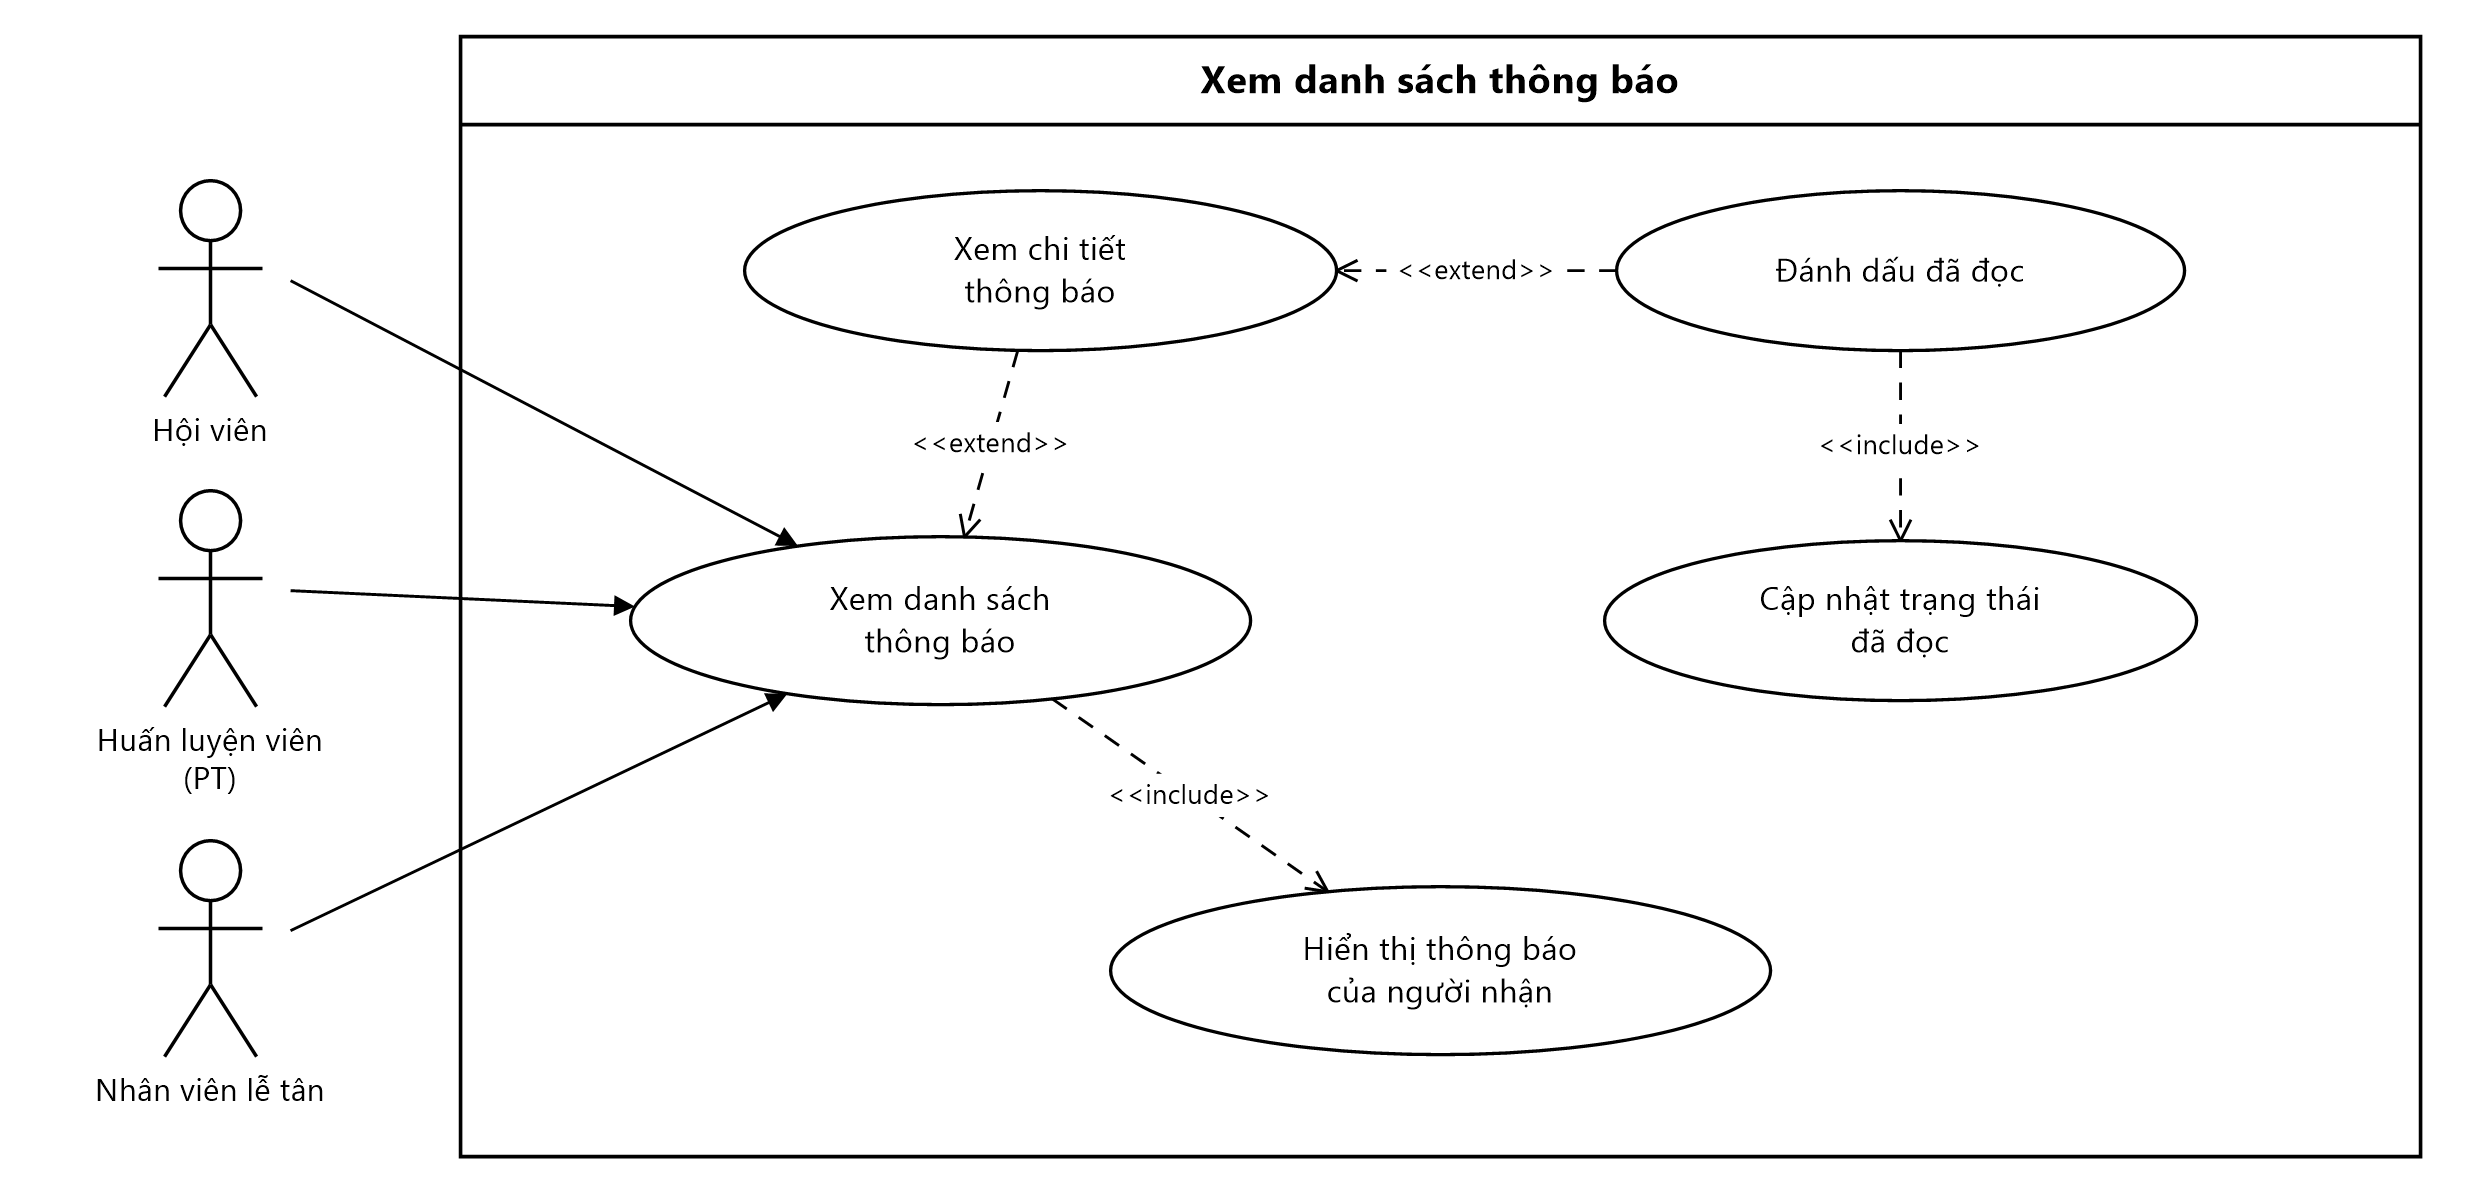
\includegraphics[width=0.88\textwidth, height=0.65\textheight, keepaspectratio]{images/uc_p40_1.png}
\caption{Use-case Xem danh sách thông báo}
\end{figure}

\begin{table}[H]\centering\footnotesize
\begin{tabularx}{\textwidth}{|L{3.2cm}|Y|}
\hline \textbf{Tóm tắt} & Hội viên, HLV hoặc Lễ tân xem lại lịch sử thông báo của mình, phân biệt đã đọc và chưa đọc. \\ \hline
\textbf{Tiền điều kiện} & Người dùng đã đăng nhập với vai trò Hội viên, Huấn luyện viên hoặc Nhân viên lễ tân. \\ \hline
\textbf{Dòng sự kiện chính} & 1. Người dùng chọn chức năng "Thông báo".\newline 2. Hệ thống hiển thị danh sách thông báo của người dùng, phân biệt đã đọc và chưa đọc.\newline 3. Người dùng chọn một thông báo để xem chi tiết; hệ thống ghi nhận trạng thái "đã đọc". \\ \hline
\textbf{Dòng sự kiện phụ} & -- Chưa có thông báo: hiển thị "Bạn chưa có thông báo nào".\newline -- Đánh dấu đã đọc từ danh sách: chọn "Đánh dấu đã đọc" ngay trên danh sách mà không mở chi tiết. \\ \hline
\textbf{Hậu điều kiện} & Chỉ hiển thị thông báo thuộc người nhận; trạng thái "đã đọc" được cập nhật chính xác. \\ \hline
\end{tabularx}
\caption{Bảng đặc tả Use-case 45: Xem danh sách thông báo}
\end{table}

\begin{table}[H]\centering\footnotesize
\begin{tabularx}{\textwidth}{|L{3.2cm}|Y|}
\hline \textbf{Tóm tắt} & Người dùng chọn một thông báo trong danh sách để xem nội dung đầy đủ của thông báo đó. \\ \hline
\textbf{Tiền điều kiện} & Người dùng đã đăng nhập; danh sách thông báo có ít nhất một thông báo. \\ \hline
\textbf{Dòng sự kiện chính} & 1. Người dùng chọn một thông báo trong danh sách.\newline 2. Hệ thống kiểm tra thông báo thuộc về người dùng hiện tại.\newline 3. Hiển thị nội dung chi tiết (loại, nội dung, thời gian gửi) và ghi nhận trạng thái "đã đọc". \\ \hline
\textbf{Dòng sự kiện phụ} & -- Thông báo không thuộc người dùng hoặc không tồn tại: không hiển thị và báo lỗi.\newline -- Đã đọc trước đó: chỉ hiển thị nội dung, không thay đổi trạng thái. \\ \hline
\textbf{Hậu điều kiện} & Hiển thị đúng nội dung thông báo và cập nhật trạng thái "đã đọc". \\ \hline
\end{tabularx}
\caption{Bảng đặc tả Use-case 46: Xem chi tiết thông báo}
\end{table}

\begin{table}[H]\centering\footnotesize
\begin{tabularx}{\textwidth}{|L{3.2cm}|Y|}
\hline \textbf{Tóm tắt} & Use-case mở rộng khi người dùng chủ động đánh dấu một thông báo là đã đọc. \\ \hline
\textbf{Tiền điều kiện} & Người dùng đã đăng nhập; thông báo thuộc về người dùng và đang ở trạng thái chưa đọc. \\ \hline
\textbf{Dòng sự kiện chính} & 1. Người dùng chọn "Đánh dấu đã đọc" trên thông báo chưa đọc.\newline 2. Hệ thống cập nhật trạng thái thành "đã đọc" và cập nhật hiển thị danh sách. \\ \hline
\textbf{Dòng sự kiện phụ} & Thông báo đã ở trạng thái đã đọc: hệ thống không thực hiện thay đổi nào. \\ \hline
\textbf{Hậu điều kiện} & Trạng thái "đã đọc" được lưu; các thông báo khác và nội dung không bị ảnh hưởng. \\ \hline
\end{tabularx}
\caption{Bảng đặc tả Use-case 47: Đánh dấu đã đọc}
\end{table}

\paragraph{19. Gửi thông báo tự động}
\begin{figure}[H]
\centering
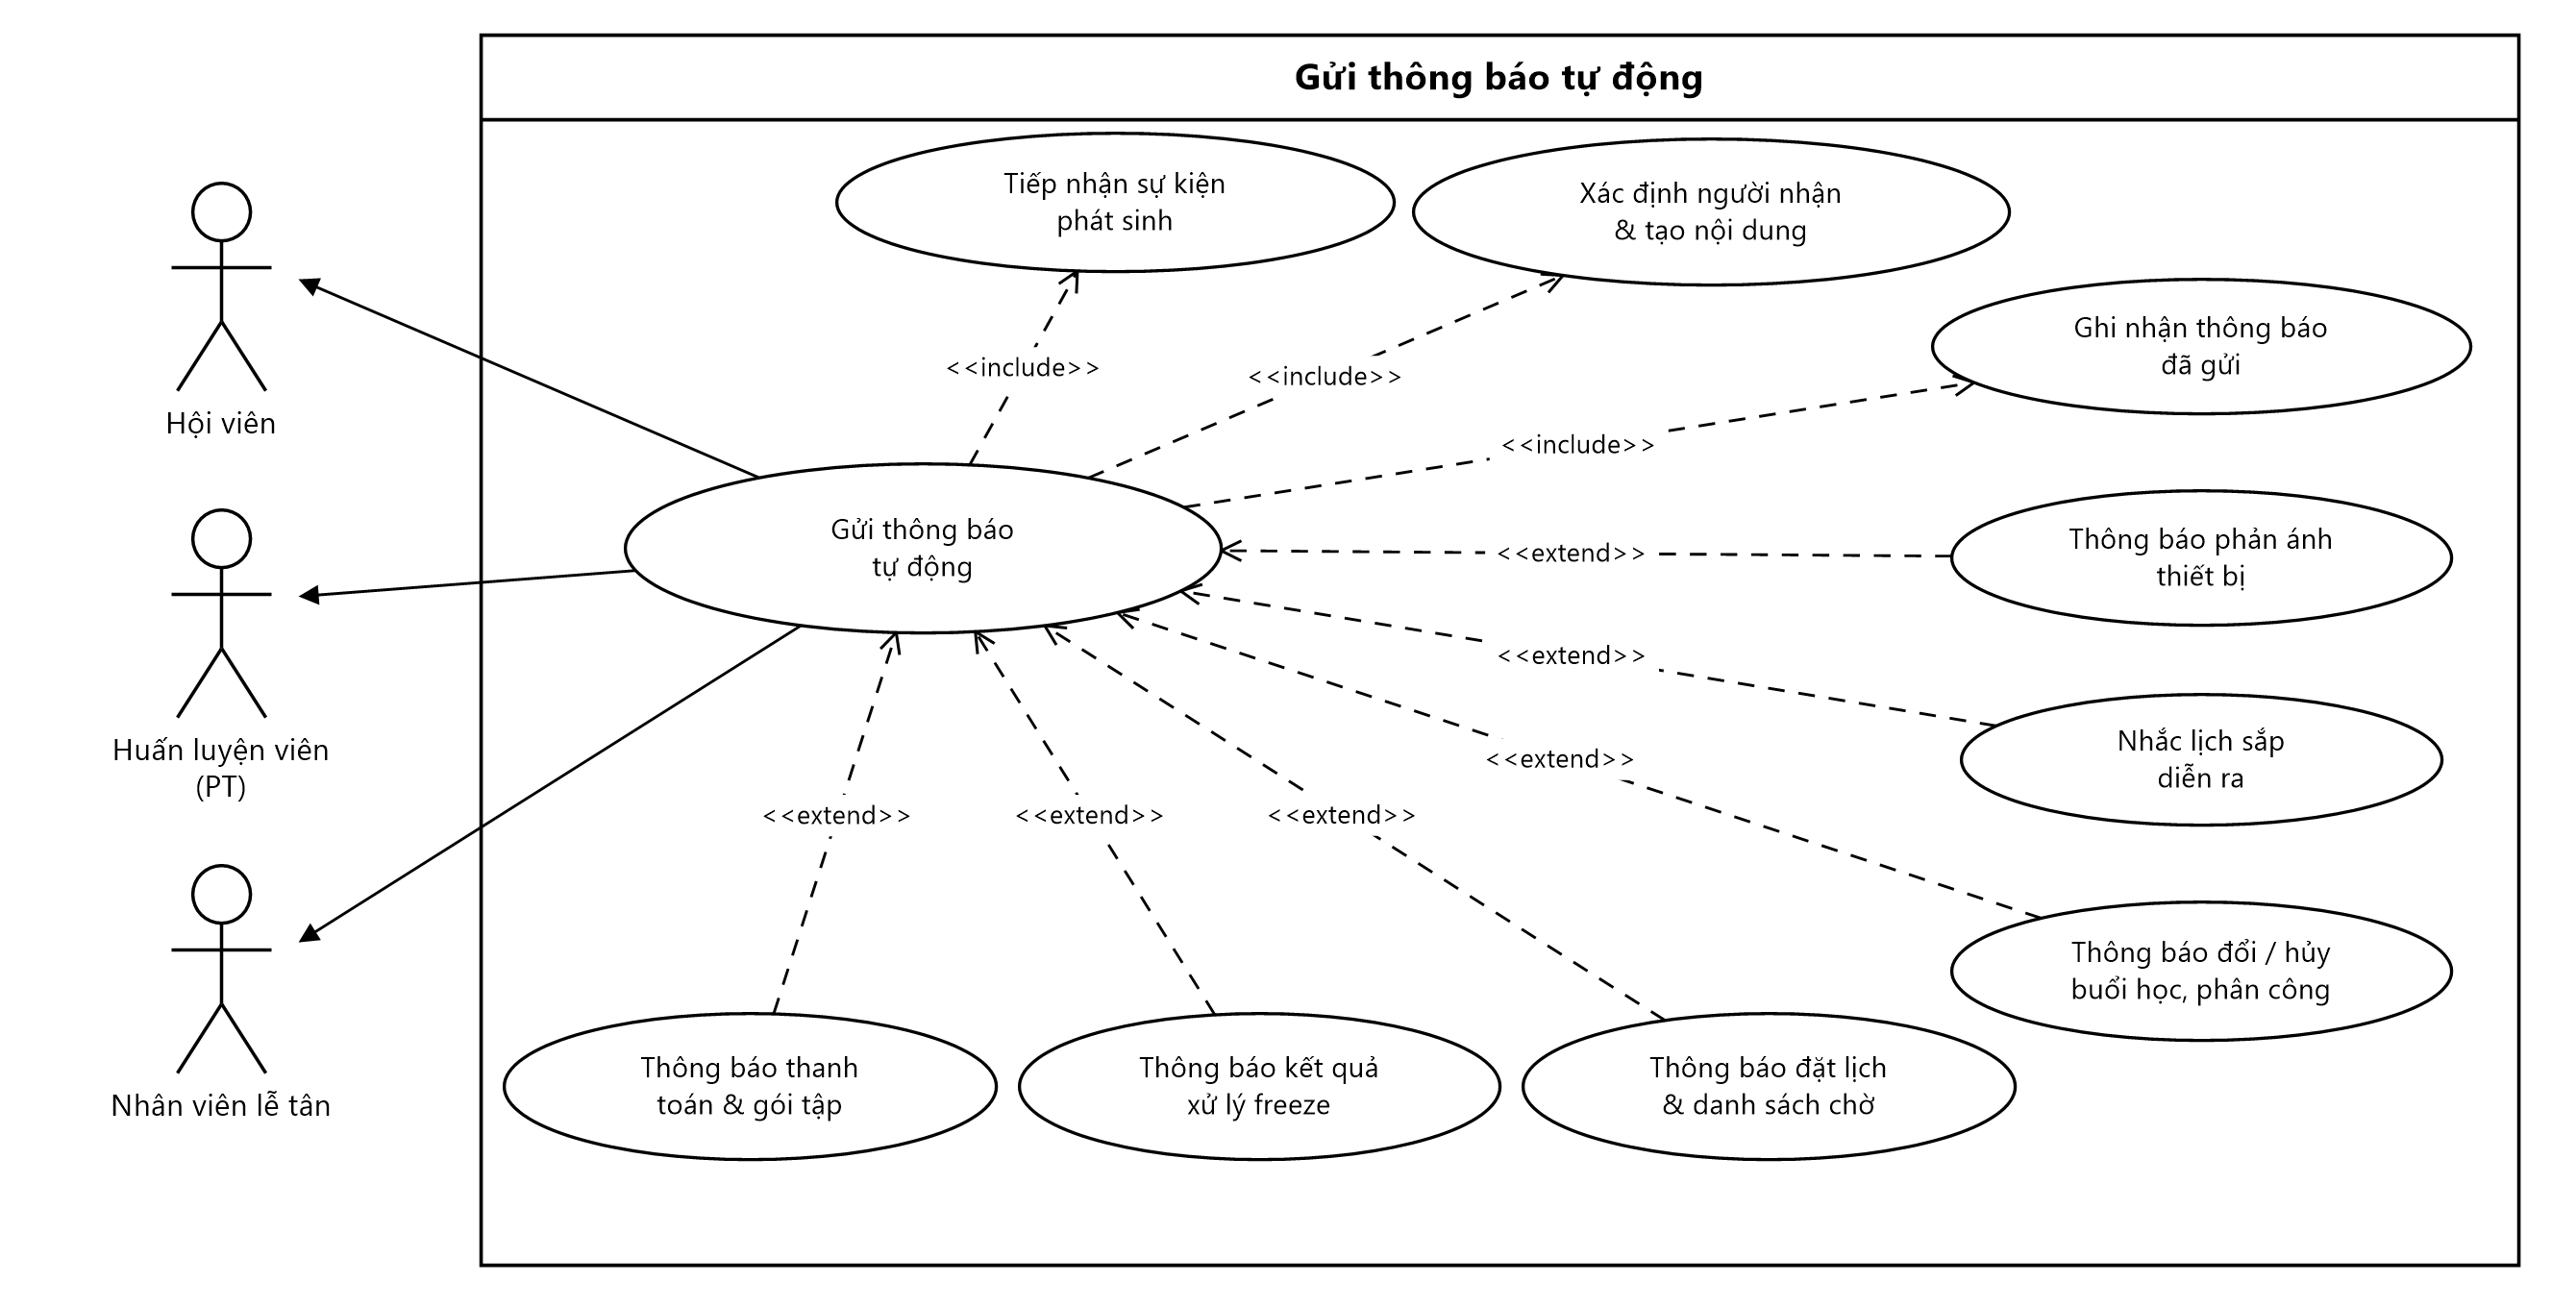
\includegraphics[width=0.88\textwidth, height=0.65\textheight, keepaspectratio]{images/uc_p43_1.png}
\caption{Use-case Gửi thông báo tự động}
\end{figure}

\begin{table}[H]\centering\footnotesize
\begin{tabularx}{\textwidth}{|L{3.2cm}|Y|}
\hline \textbf{Tóm tắt} & Khi phát sinh sự kiện (thanh toán, freeze, đặt lịch, sự cố thiết bị...) hoặc đến mốc nhắc lịch, hệ thống tự động tạo và gửi thông báo đến người nhận phù hợp. \\ \hline
\textbf{Tiền điều kiện} & Có sự kiện phát sinh cần thông báo hoặc đến thời điểm nhắc lịch; người nhận có tài khoản hợp lệ. \\ \hline
\textbf{Dòng sự kiện chính} & 1. Tiếp nhận sự kiện phát sinh cùng thông tin cần thiết.\newline 2. Xác định loại thông báo và đối tượng nhận (Hội viên, HLV, Lễ tân) theo quy tắc.\newline 3. Tạo nội dung phù hợp, gửi thông báo và ghi nhận vào lịch sử thông báo. \\ \hline
\textbf{Dòng sự kiện phụ} & -- Thiếu thông tin sự kiện: không tạo thông báo.\newline -- Nhắc lịch sắp diễn ra: tự phát sinh trước giờ học (mặc định 2 giờ).\newline -- Sự kiện nhiều người nhận (hủy/đổi lớp): gửi đến từng HLV và Hội viên liên quan. \\ \hline
\textbf{Hậu điều kiện} & Thông báo được gửi đúng người nhận và lưu lại trong danh sách thông báo. \\ \hline
\end{tabularx}
\caption{Bảng đặc tả Use-case 48: Gửi thông báo tự động}
\end{table}

\begin{table}[H]\centering\footnotesize
\begin{tabularx}{\textwidth}{|L{3.2cm}|Y|}
\hline \textbf{Tóm tắt} & Use-case mở rộng thông báo cho Hội viên về kết quả thanh toán, gói tập sắp hết hạn hoặc gói PT sắp hết buổi. \\ \hline
\textbf{Tiền điều kiện} & Hội viên đã thực hiện thanh toán hoặc đang sở hữu gói tập còn hiệu lực. \\ \hline
\textbf{Dòng sự kiện chính} & 1. Tiếp nhận sự kiện thanh toán (thành công/thất bại) hoặc cảnh báo sắp hết hạn/hết buổi.\newline 2. Xác định Hội viên sở hữu giao dịch/gói tập là người nhận.\newline 3. Tạo nội dung tương ứng (kết quả, thời hạn/số buổi còn lại), gửi và lưu thông báo. \\ \hline
\textbf{Dòng sự kiện phụ} & Thanh toán thất bại: thông báo cho biết gói chưa kích hoạt và có thể thanh toán lại. \\ \hline
\textbf{Hậu điều kiện} & Hội viên nhận được thông báo đúng với kết quả thanh toán hoặc tình trạng gói tập. \\ \hline
\end{tabularx}
\caption{Bảng đặc tả Use-case 49: Thông báo thanh toán \& gói tập}
\end{table}

\begin{table}[H]\centering\footnotesize
\begin{tabularx}{\textwidth}{|L{3.2cm}|Y|}
\hline \textbf{Tóm tắt} & Thông báo cho Nhân viên lễ tân khi có yêu cầu freeze mới, và thông báo cho Hội viên kết quả duyệt/từ chối cùng các lịch bị hủy do freeze. \\ \hline
\textbf{Tiền điều kiện} & Hội viên đã gửi yêu cầu freeze hoặc yêu cầu freeze đã được Lễ tân xử lý. \\ \hline
\textbf{Dòng sự kiện chính} & 1. Tiếp nhận sự kiện freeze (yêu cầu mới, duyệt/từ chối, hủy lịch tự động).\newline 2. Xác định người nhận (Lễ tân khi có yêu cầu mới; Hội viên khi có kết quả).\newline 3. Tạo nội dung, gửi và ghi nhận thông báo. \\ \hline
\textbf{Dòng sự kiện phụ} & -- Yêu cầu bị từ chối: nêu rõ yêu cầu không được chấp thuận.\newline -- Có lịch trùng khoảng freeze: gửi thêm thông báo các lịch bị hủy và lượt hoàn lại. \\ \hline
\textbf{Hậu điều kiện} & Lễ tân biết có yêu cầu cần xử lý; Hội viên nhận được kết quả xử lý freeze. \\ \hline
\end{tabularx}
\caption{Bảng đặc tả Use-case 50: Thông báo kết quả xử lý freeze}
\end{table}

\begin{table}[H]\centering\footnotesize
\begin{tabularx}{\textwidth}{|L{3.2cm}|Y|}
\hline \textbf{Tóm tắt} & Thông báo cho Hội viên khi lịch được xác nhận, đôn từ Waitlist vào lớp hoặc lớp đầy, và thông báo cho HLV khi có yêu cầu đặt lịch riêng. \\ \hline
\textbf{Tiền điều kiện} & Hội viên đã đặt lớp nhóm, đang trong Waitlist hoặc đã gửi yêu cầu đặt lịch PT 1-kèm-1. \\ \hline
\textbf{Dòng sự kiện chính} & 1. Tiếp nhận sự kiện đặt lịch (xác nhận, đôn Waitlist, lớp đầy, đặt lịch PT).\newline 2. Xác định người nhận (Hội viên đặt lịch hoặc HLV được đặt).\newline 3. Tạo nội dung, gửi và ghi nhận thông báo. \\ \hline
\textbf{Dòng sự kiện phụ} & Lớp đã đầy ở mốc $T-8h$: thông báo cho hội viên trong Waitlist chọn lịch khác. \\ \hline
\textbf{Hậu điều kiện} & Hội viên hoặc HLV nhận được thông báo đúng với trạng thái đặt lịch. \\ \hline
\end{tabularx}
\caption{Bảng đặc tả Use-case 51: Thông báo đặt lịch \& danh sách chờ}
\end{table}

\begin{table}[H]\centering\footnotesize
\begin{tabularx}{\textwidth}{|L{3.2cm}|Y|}
\hline \textbf{Tóm tắt} & Thông báo cho HLV và Hội viên liên quan khi Admin phân công lớp hoặc khi buổi học, lịch hẹn 1-kèm-1 bị đổi/hủy. \\ \hline
\textbf{Tiền điều kiện} & Lớp học đã được phân công hoặc buổi học, lịch hẹn đã được đổi hoặc hủy trên hệ thống. \\ \hline
\textbf{Dòng sự kiện chính} & 1. Tiếp nhận sự kiện phân công HLV hoặc đổi/hủy buổi học, lịch hẹn.\newline 2. Xác định người nhận (HLV phụ trách và các Hội viên đã đăng ký).\newline 3. Tạo nội dung nêu rõ buổi học và thay đổi, gửi và ghi nhận thông báo. \\ \hline
\textbf{Dòng sự kiện phụ} & Phân công lớp mới: thông báo chỉ gửi đến HLV được phân công. \\ \hline
\textbf{Hậu điều kiện} & HLV và Hội viên liên quan nhận được thông báo về thay đổi trong danh sách thông báo. \\ \hline
\end{tabularx}
\caption{Bảng đặc tả Use-case 52: Thông báo đổi / hủy buổi học, phân công}
\end{table}

\begin{table}[H]\centering\footnotesize
\begin{tabularx}{\textwidth}{|L{3.2cm}|Y|}
\hline \textbf{Tóm tắt} & Tự động nhắc Hội viên và HLV về buổi học hoặc lịch hẹn sắp diễn ra trước giờ bắt đầu theo khoảng thời gian cấu hình. \\ \hline
\textbf{Tiền điều kiện} & Hội viên có lịch đặt lớp nhóm hoặc PT đã xác nhận; đã cấu hình khoảng thời gian nhắc lịch. \\ \hline
\textbf{Dòng sự kiện chính} & 1. Hệ thống phát hiện buổi học/lịch hẹn đến mốc nhắc lịch (mặc định 2 giờ trước giờ bắt đầu).\newline 2. Xác định người nhận (Hội viên có lịch đặt và HLV phụ trách).\newline 3. Tạo nội dung nhắc lịch (loại buổi, thời gian, chi nhánh), gửi và lưu thông báo. \\ \hline
\textbf{Dòng sự kiện phụ} & Lịch đã bị hủy hoặc thay đổi trước mốc nhắc: hệ thống không gửi nhắc lịch cũ. \\ \hline
\textbf{Hậu điều kiện} & Hội viên và HLV nhận được thông báo nhắc lịch đúng khoảng thời gian cấu hình. \\ \hline
\end{tabularx}
\caption{Bảng đặc tả Use-case 53: Nhắc lịch sắp diễn ra}
\end{table}

\begin{table}[H]\centering\footnotesize
\begin{tabularx}{\textwidth}{|L{3.2cm}|Y|}
\hline \textbf{Tóm tắt} & Tự động thông báo cho Nhân viên lễ tân khi có phản ánh thiết bị hỏng cần tiếp nhận và xử lý. \\ \hline
\textbf{Tiền điều kiện} & Có phản ánh thiết bị hỏng được ghi nhận trên hệ thống. \\ \hline
\textbf{Dòng sự kiện chính} & 1. Tiếp nhận sự kiện có phản ánh thiết bị cần xử lý.\newline 2. Xác định Nhân viên phụ trách chi nhánh có thiết bị được phản ánh.\newline 3. Tạo nội dung nêu thiết bị và chi nhánh liên quan, gửi và lưu thông báo. \\ \hline
\textbf{Dòng sự kiện phụ} & Thông tin thiết bị không đầy đủ: hệ thống không tạo thông báo. \\ \hline
\textbf{Hậu điều kiện} & Nhân viên nhận được thông báo về thiết bị cần xử lý trong danh sách thông báo. \\ \hline
\end{tabularx}
\caption{Bảng đặc tả Use-case 54: Thông báo phản ánh thiết bị}
\end{table}

\paragraph{20. Bảo lưu / Tạm ngưng gói tập (Freeze)}
\begin{figure}[H]
\centering
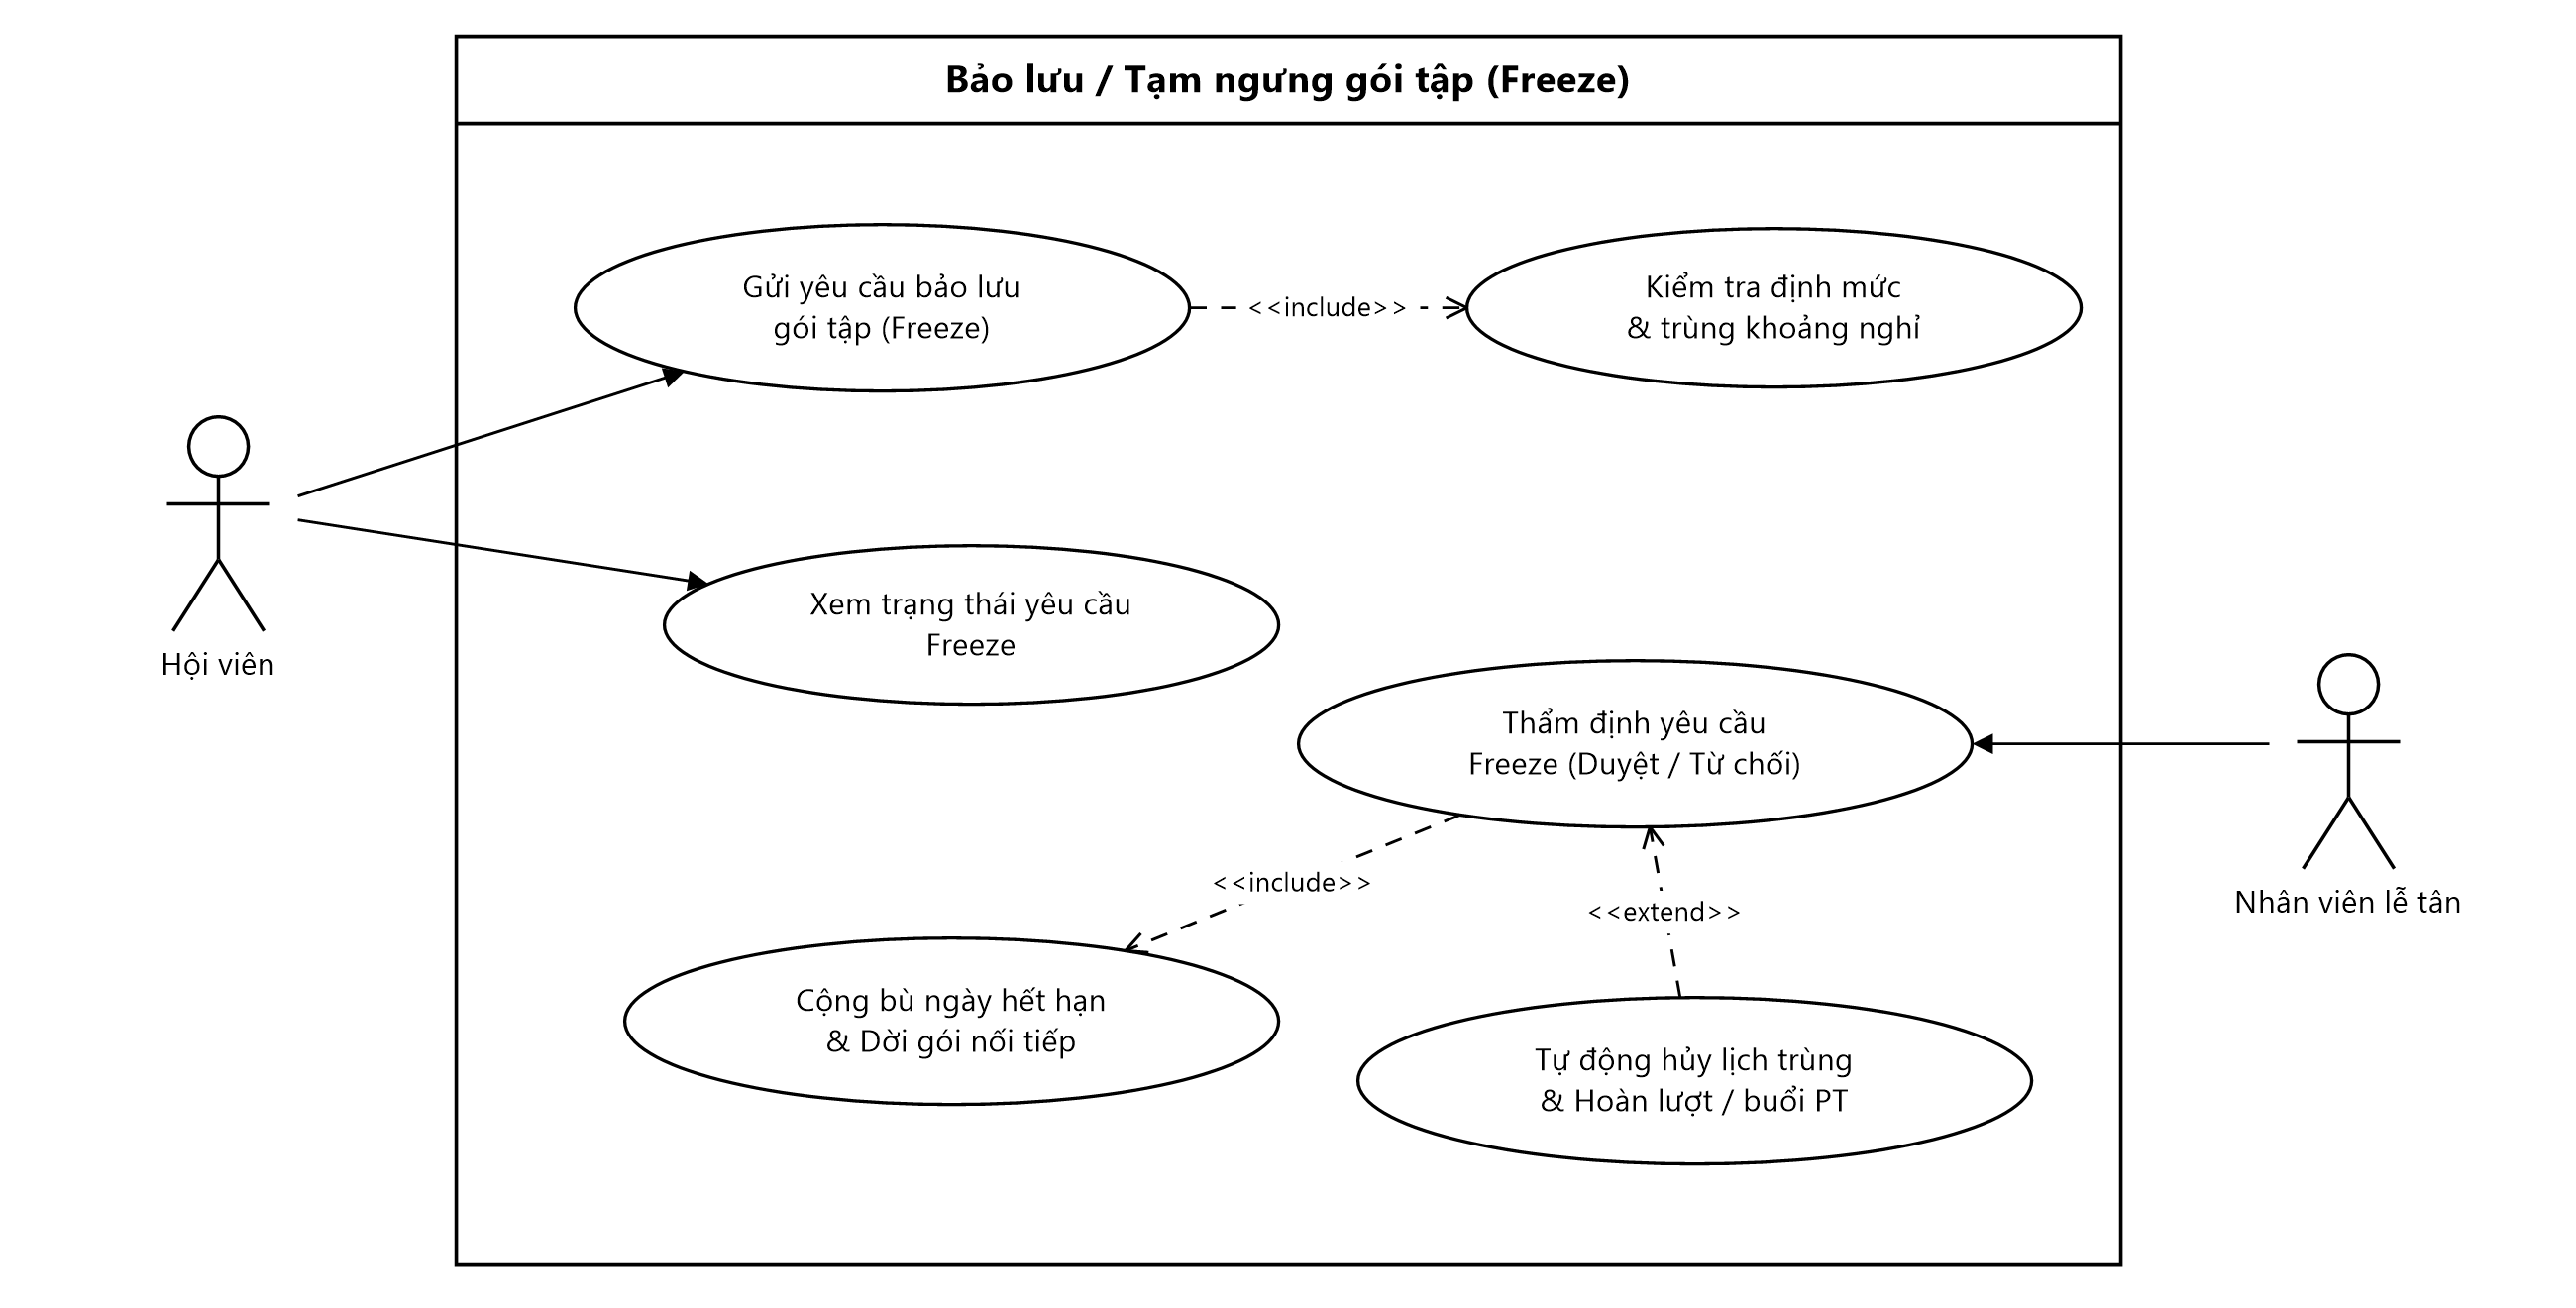
\includegraphics[width=0.88\textwidth, height=0.65\textheight, keepaspectratio]{images/uc_freeze.png}
\caption{Use-case Bảo lưu / Tạm ngưng gói tập (Freeze)}
\end{figure}

\begin{table}[H]\centering\footnotesize
\begin{tabularx}{\textwidth}{|L{3.2cm}|Y|}
\hline \textbf{Tóm tắt} & Hội viên gửi đơn đề nghị tạm ngưng gói hội viên đang hiệu lực trong khoảng thời gian xác định theo định mức của gói. \\ \hline
\textbf{Tiền điều kiện} & Hội viên đã đăng nhập; đang sở hữu gói hội viên (\texttt{MEMBERSHIP}) hiệu lực có hỗ trợ Freeze (\texttt{Max\_Freeze\_Times} $> 0$) và chưa có yêu cầu \texttt{Pending}. \\ \hline
\textbf{Dòng sự kiện chính} & 1. Hội viên truy cập mục bảo lưu gói tập (\texttt{/member/freeze}), chọn gói đang sử dụng.\newline 2. Nhập ngày bắt đầu tạm ngưng (sau ngày hiện tại), số ngày tạm ngưng và lý do.\newline 3. Hệ thống kiểm tra giới hạn số lần (\texttt{Max\_Freeze\_Times}), tổng số ngày (\texttt{Max\_Freeze\_Days}) và không trùng với đợt Freeze đã duyệt trước đó.\newline 4. Lưu yêu cầu trạng thái \texttt{Pending} và gửi thông báo đến Nhân viên lễ tân chờ thẩm định. \\ \hline
\textbf{Dòng sự kiện phụ} & -- Vượt quá số lần hoặc số ngày bảo lưu còn lại, ngày bắt đầu không hợp lệ hoặc trùng lịch Freeze đã duyệt $\rightarrow$ hệ thống từ chối và hiển thị thông báo lỗi.\newline -- Gói PT 1-kèm-1 không áp dụng cơ chế Freeze. \\ \hline
\textbf{Hậu điều kiện} & Yêu cầu Freeze được ghi nhận ở trạng thái \texttt{Pending} và thông báo được gửi tới quầy lễ tân. \\ \hline
\end{tabularx}
\caption{Bảng đặc tả Use-case 55: Gửi yêu cầu bảo lưu gói tập (Freeze)}
\end{table}

\begin{table}[H]\centering\footnotesize
\begin{tabularx}{\textwidth}{|L{3.2cm}|Y|}
\hline \textbf{Tóm tắt} & Nhân viên lễ tân xem xét hồ sơ yêu cầu bảo lưu đang chờ duyệt và quyết định Chấp thuận (Approved) hoặc Từ chối (Rejected). \\ \hline
\textbf{Tiền điều kiện} & Nhân viên lễ tân đã đăng nhập; tồn tại ít nhất một yêu cầu Freeze ở trạng thái \texttt{Pending}. \\ \hline
\textbf{Dòng sự kiện chính} & 1. Lễ tân mở danh sách yêu cầu bảo lưu (\texttt{/staff/freeze}) tại tab \textit{Chờ duyệt}.\newline 2. Kiểm tra thông tin hội viên, khoảng ngày bảo lưu và lý do.\newline 3. Chọn "Duyệt yêu cầu"; hệ thống chuyển trạng thái sang \texttt{Approved}, tự động cộng bù số ngày vào \texttt{End\_Date} gói hiện tại và dời ngày các gói nối tiếp.\newline 4. Hệ thống tự động hủy các lịch lớp nhóm/PT trùng trong khoảng Freeze, hoàn lượt/buổi PT (đôn Waitlist nếu còn chỗ trống lớp nhóm) và gửi thông báo kết quả cho Hội viên. \\ \hline
\textbf{Dòng sự kiện phụ} & Nếu Lễ tân chọn "Từ chối" kèm ghi chú lý do: yêu cầu chuyển sang \texttt{Rejected}, không cộng bù hạn gói và gửi thông báo lý do từ chối cho Hội viên. \\ \hline
\textbf{Hậu điều kiện} & Yêu cầu Freeze chuyển sang \texttt{Approved} hoặc \texttt{Rejected}; thời hạn gói và các lịch đặt liên quan được cập nhật nhất quán. \\ \hline
\end{tabularx}
\caption{Bảng đặc tả Use-case 56: Thẩm định yêu cầu bảo lưu gói tập (Freeze)}
\end{table}

\paragraph{21. Quản lý Thẻ hội viên (MemberCard)}
\begin{figure}[H]
\centering
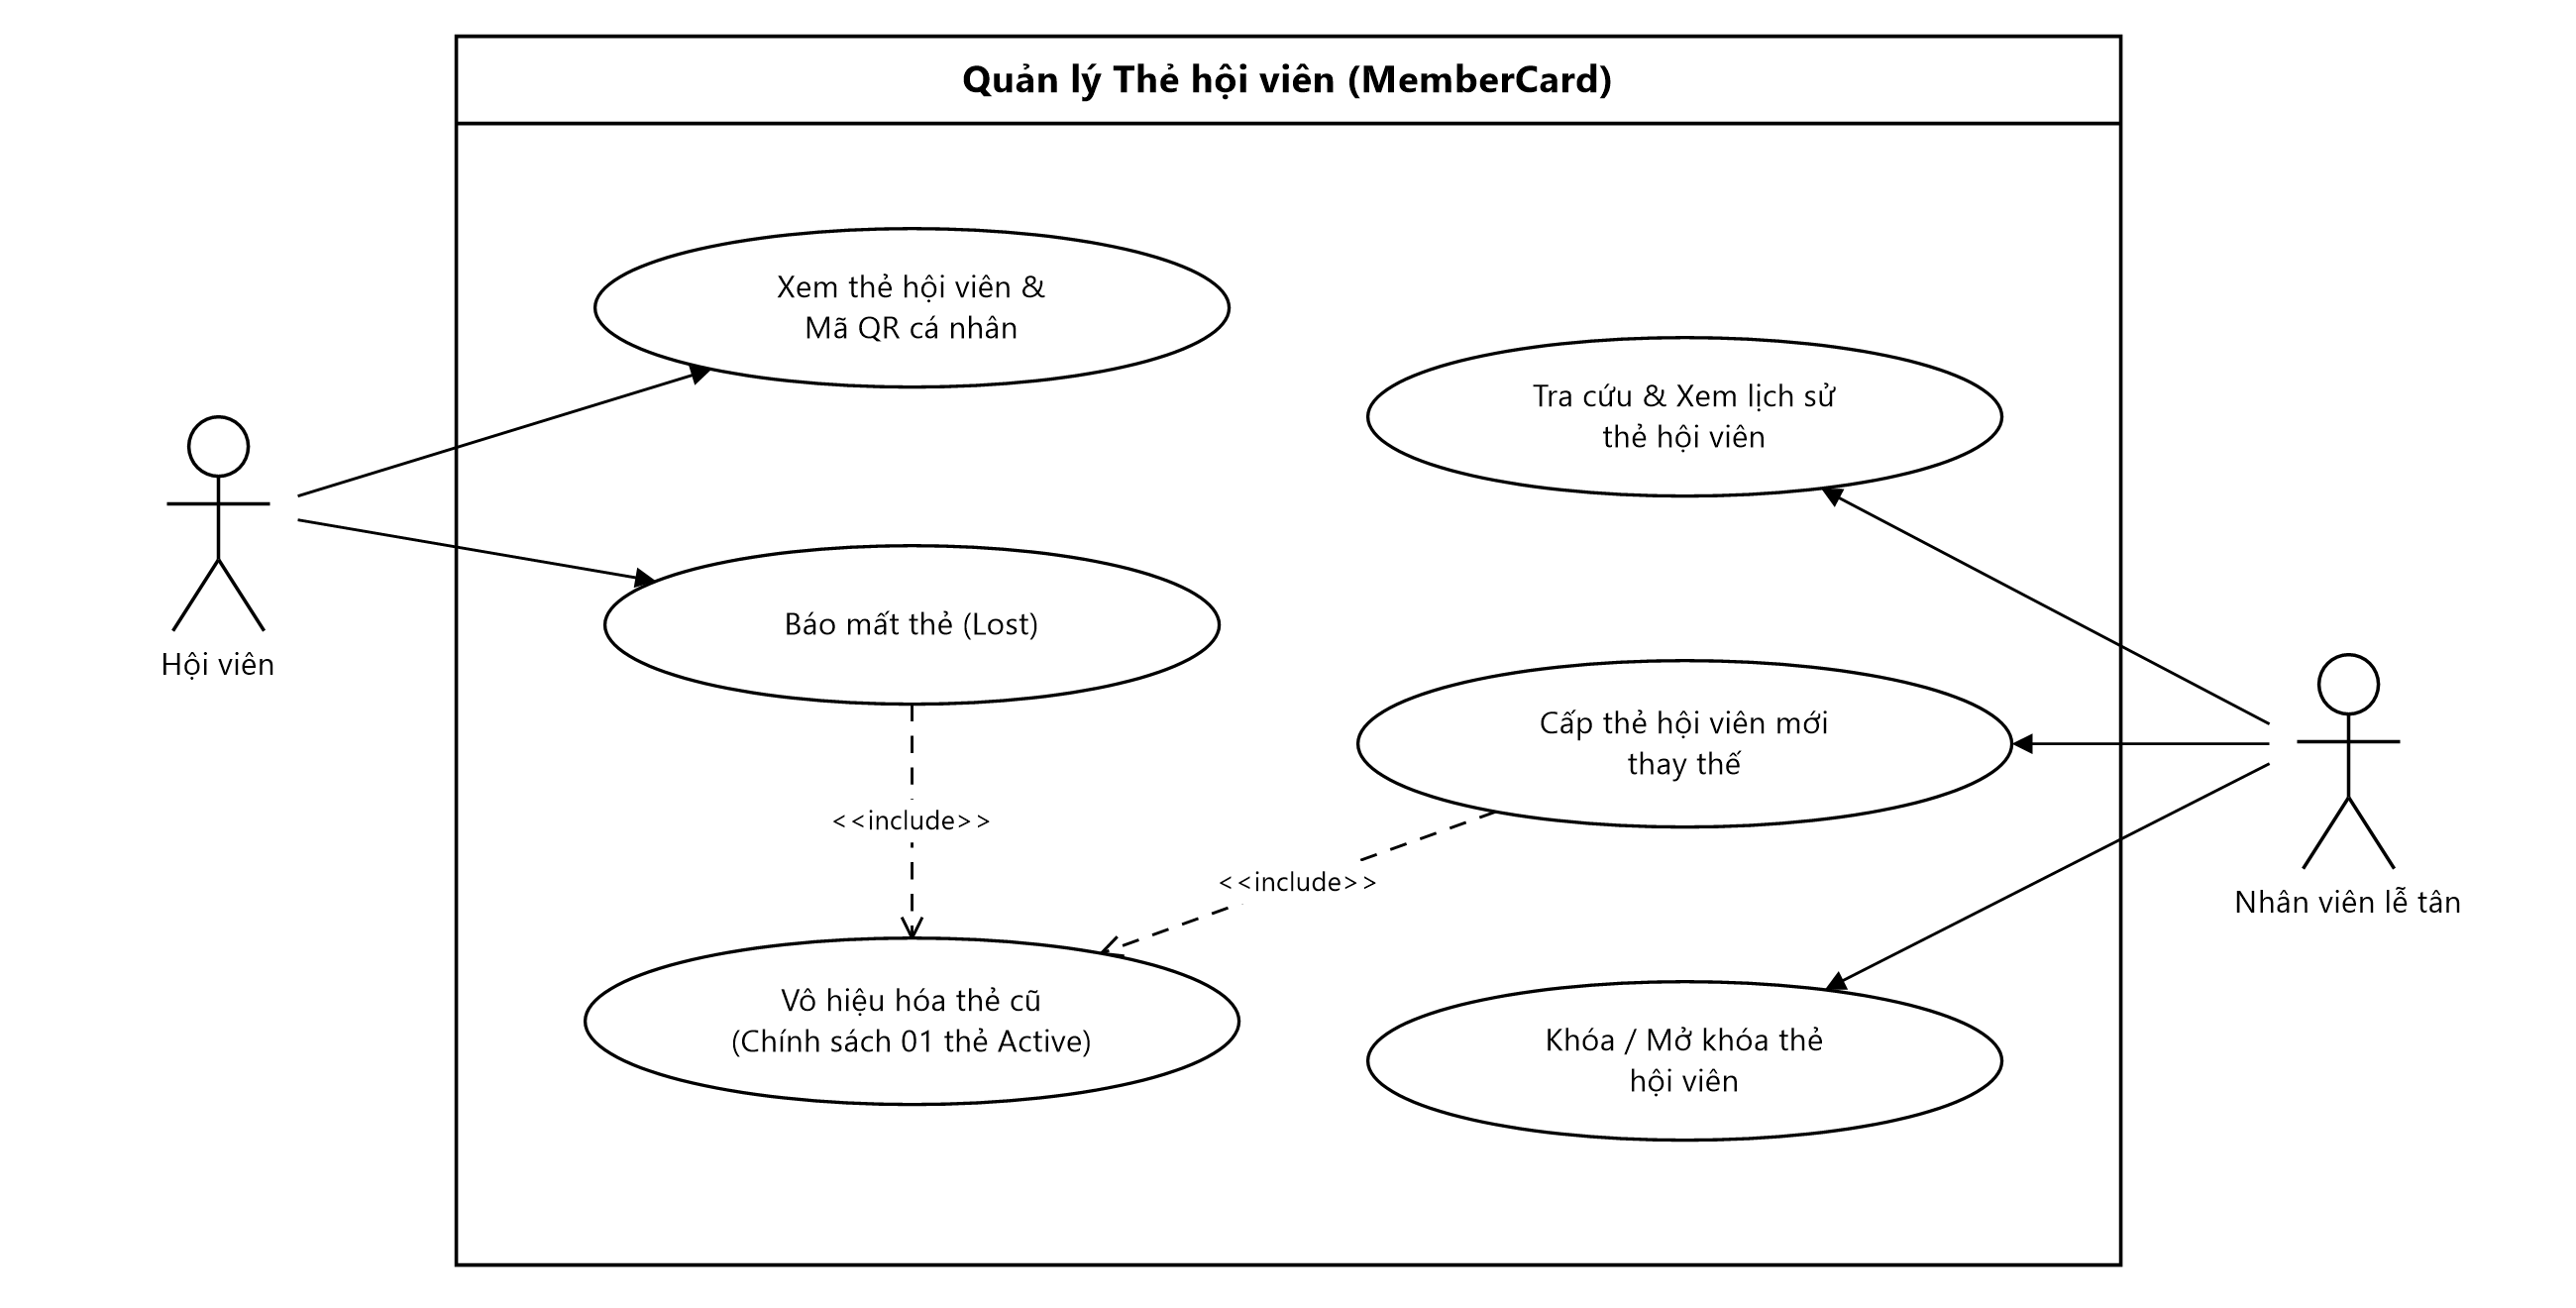
\includegraphics[width=0.88\textwidth, height=0.65\textheight, keepaspectratio]{images/uc_member_card.png}
\caption{Use-case Quản lý Thẻ hội viên (MemberCard)}
\end{figure}

\begin{table}[H]\centering\footnotesize
\begin{tabularx}{\textwidth}{|L{3.2cm}|Y|}
\hline \textbf{Tóm tắt} & Hội viên xem mã thẻ và mã QR cá nhân phục vụ check-in hoặc chủ động báo mất thẻ khi bị thất lạc để vô hiệu hóa thẻ ngay lập tức. \\ \hline
\textbf{Tiền điều kiện} & Hội viên đã đăng nhập; tài khoản đã được cấp thẻ thành viên. \\ \hline
\textbf{Dòng sự kiện chính} & 1. Hội viên mở trang Thẻ hội viên \& Mã QR (\texttt{/member/card} hoặc \texttt{/member/profile}) để xem mã thẻ, mã QR và lịch sử thẻ.\newline 2. Khi thất lạc thẻ, Hội viên nhấn "Báo mất thẻ" và xác nhận thao tác.\newline 3. Hệ thống chuyển trạng thái thẻ thành \texttt{Lost} (vô hiệu hóa vĩnh viễn tại mọi cổng kiểm soát).\newline 4. Hệ thống gửi thông báo cho Hội viên và cảnh báo cho Nhân viên lễ tân tiếp nhận cấp thẻ mới. \\ \hline
\textbf{Dòng sự kiện phụ} & Thẻ đã ở trạng thái \texttt{Lost} thì không thể mở khóa lại mà phải chờ Lễ tân cấp thẻ mới thay thế. \\ \hline
\textbf{Hậu điều kiện} & Mã thẻ cũ bị vô hiệu hóa hoàn toàn; Nhân viên lễ tân nhận được thông báo để cấp lại thẻ mới. \\ \hline
\end{tabularx}
\caption{Bảng đặc tả Use-case 57: Xem thẻ QR \& Báo mất thẻ hội viên}
\end{table}

\begin{table}[H]\centering\footnotesize
\begin{tabularx}{\textwidth}{|L{3.2cm}|Y|}
\hline \textbf{Tóm tắt} & Nhân viên lễ tân tra cứu lịch sử thẻ và thực hiện khóa, mở khóa hoặc cấp thẻ mới thay thế cho hội viên theo chính sách tối đa 01 thẻ \texttt{Active}. \\ \hline
\textbf{Tiền điều kiện} & Nhân viên lễ tân đã đăng nhập; tài khoản hội viên tồn tại trên hệ thống. \\ \hline
\textbf{Dòng sự kiện chính} & 1. Lễ tân truy cập trang Quản lý thẻ hội viên (\texttt{/staff/member-cards}), tìm kiếm theo tên/SĐT/mã thẻ.\newline 2. Chọn thao tác phù hợp: Khóa tạm thời (\texttt{Locked}), Mở khóa lại thẻ đang \texttt{Locked} thành \texttt{Active}, hoặc Cấp thẻ mới thay thế.\newline 3. Khi cấp thẻ mới, hệ thống tự động vô hiệu hóa toàn bộ thẻ \texttt{Active} trước đó (chuyển \texttt{Locked}/\texttt{Lost}) và sinh mã thẻ ngẫu nhiên mới ở trạng thái \texttt{Active}.\newline 4. Gửi thông báo cập nhật trạng thái/mã thẻ mới cho Hội viên. \\ \hline
\textbf{Dòng sự kiện phụ} & Nếu Lễ tân cố mở khóa một thẻ đã ở trạng thái \texttt{Lost}, hệ thống từ chối và yêu cầu thực hiện chức năng "Cấp thẻ mới". \\ \hline
\textbf{Hậu điều kiện} & Mỗi hội viên chỉ có duy nhất 01 thẻ ở trạng thái \texttt{Active}; lịch sử thay đổi thẻ được lưu đầy đủ. \\ \hline
\end{tabularx}
\caption{Bảng đặc tả Use-case 58: Cấp mới / Khóa / Mở khóa thẻ hội viên}
\end{table}

\subsection{Sơ đồ tuần tự (Sequence Diagram)}
Hệ thống được mô hình hóa tương tác theo thời gian giữa các đối tượng biên (Boundary), điều khiển (Control) và thực thể (Entity) qua \textbf{26 Sequence Diagram} cho các luồng nghiệp vụ trọng tâm:

\subsubsection{Nhóm luồng Lớp học nhóm \& Điểm danh}

\begin{figure}[H]
\centering
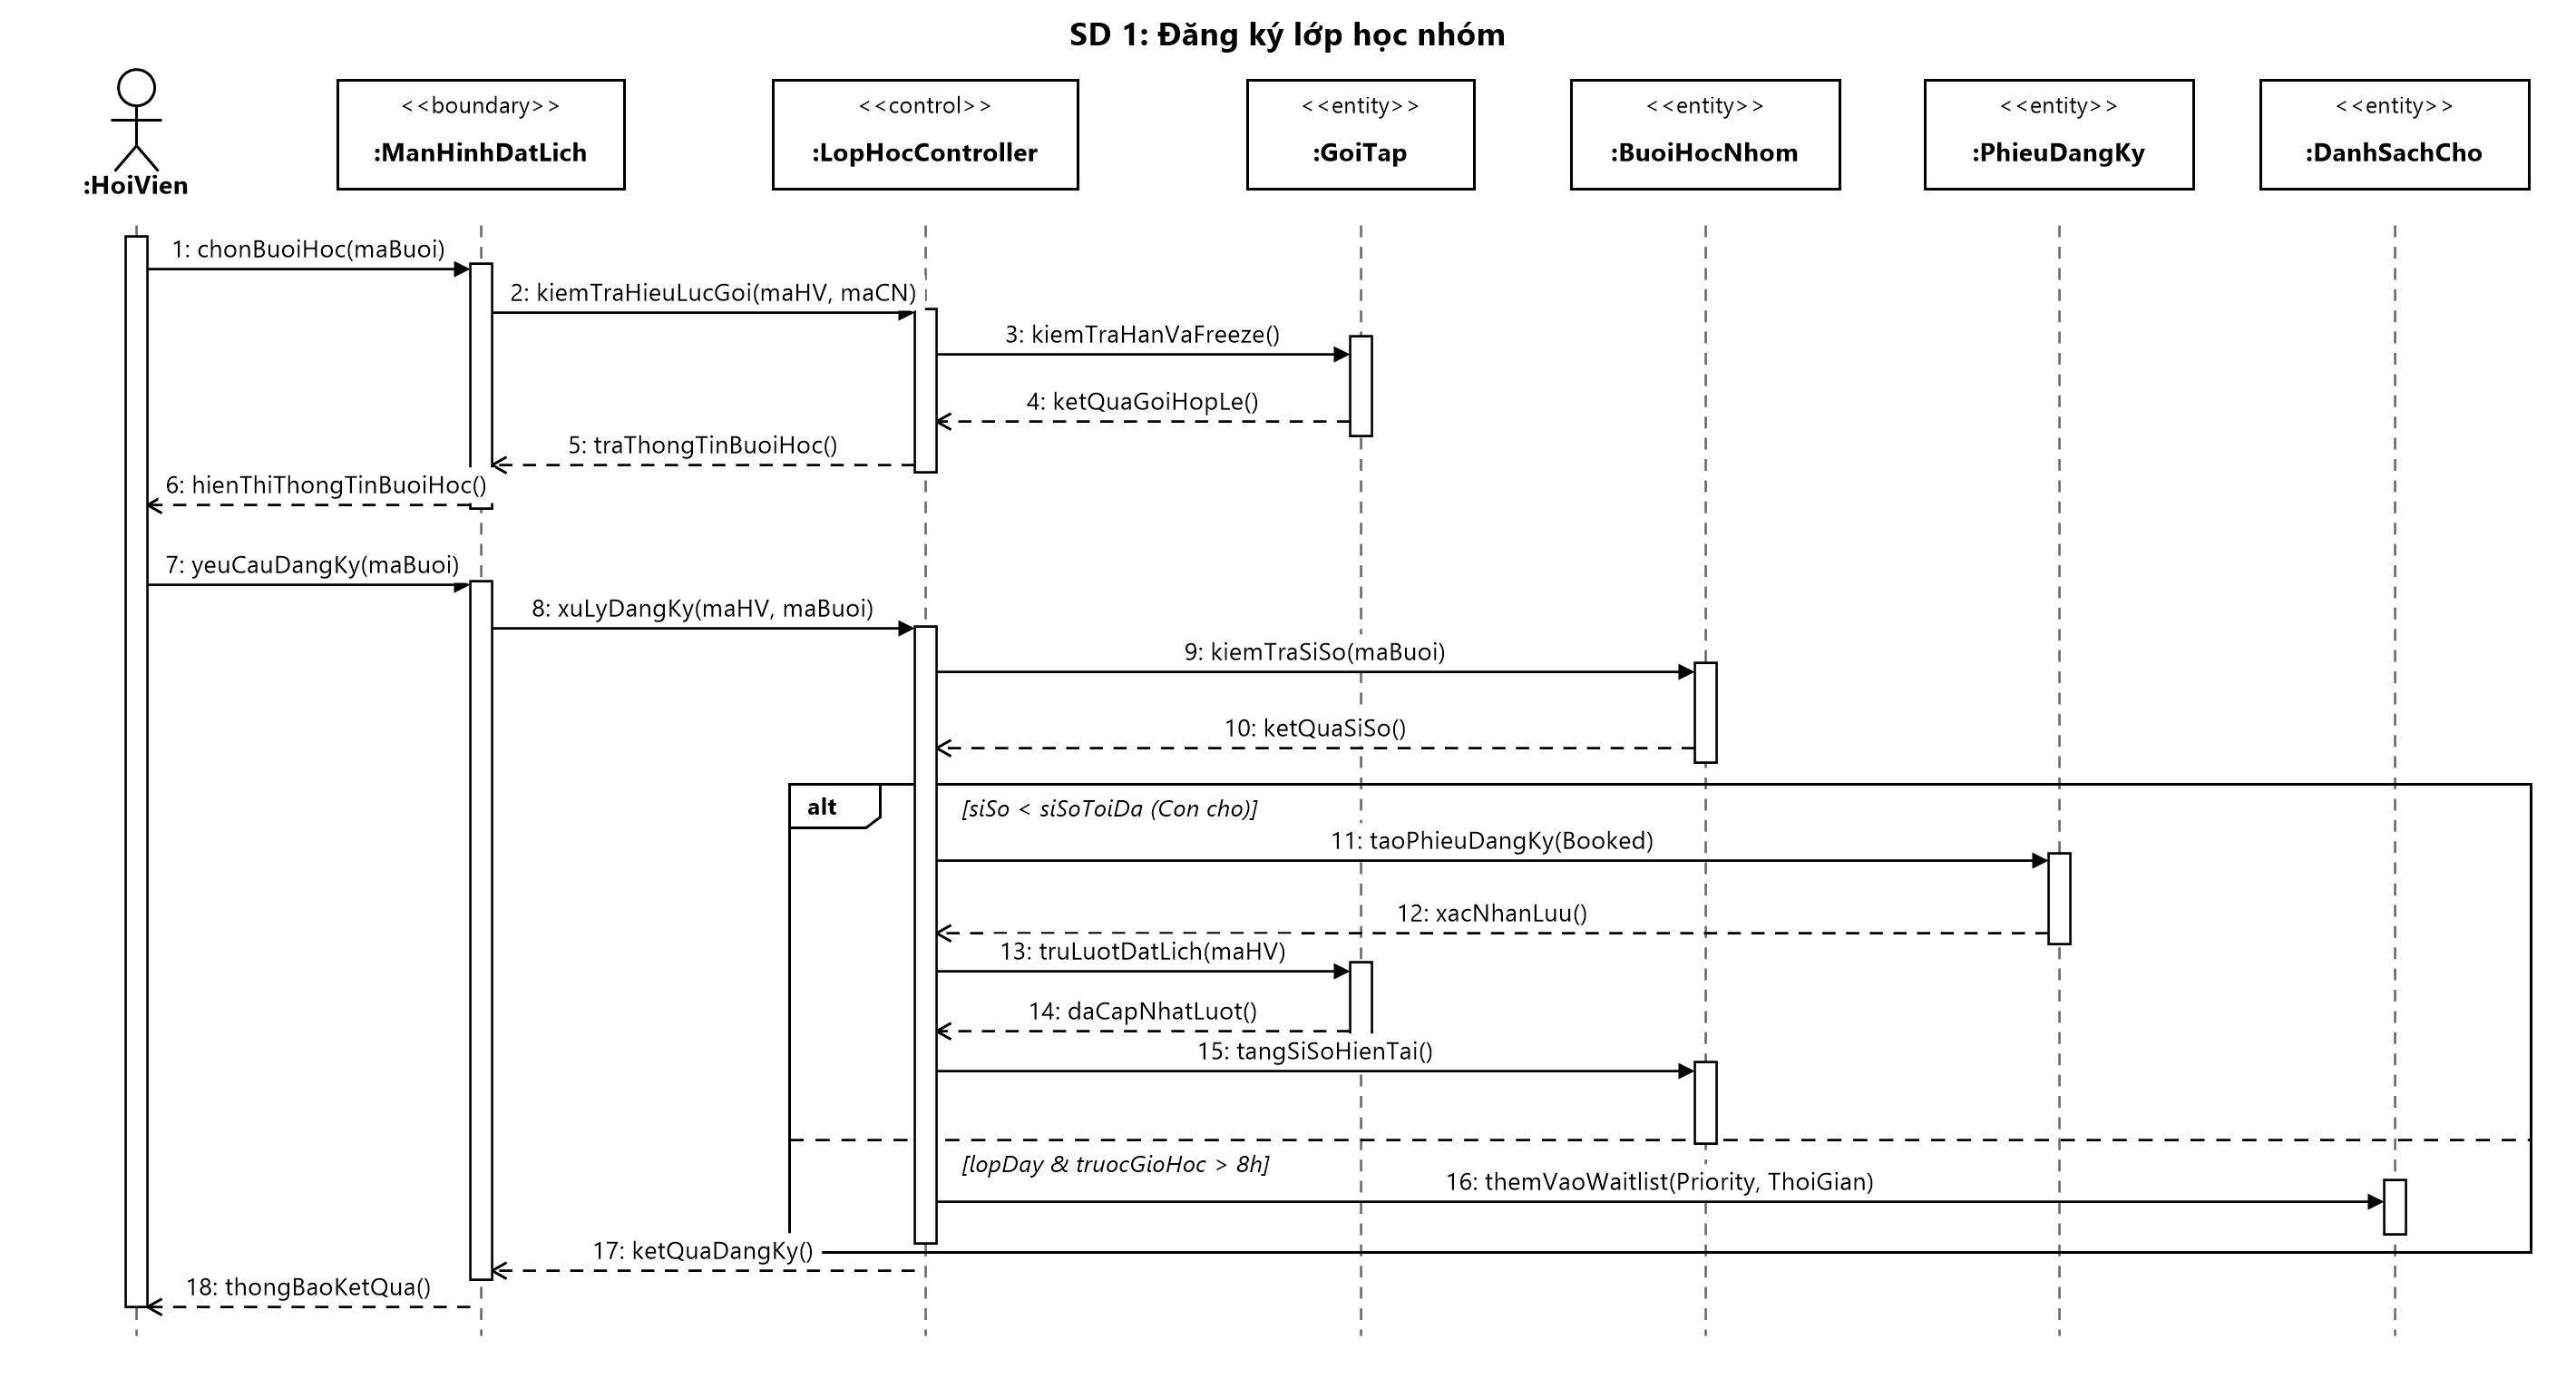
\includegraphics[width=0.95\textwidth, height=0.78\textheight, keepaspectratio]{images/sd_p50_1.png}
\caption{Sequence Diagram 1: Đăng ký lớp học nhóm}
\end{figure}

\begin{figure}[H]
\centering
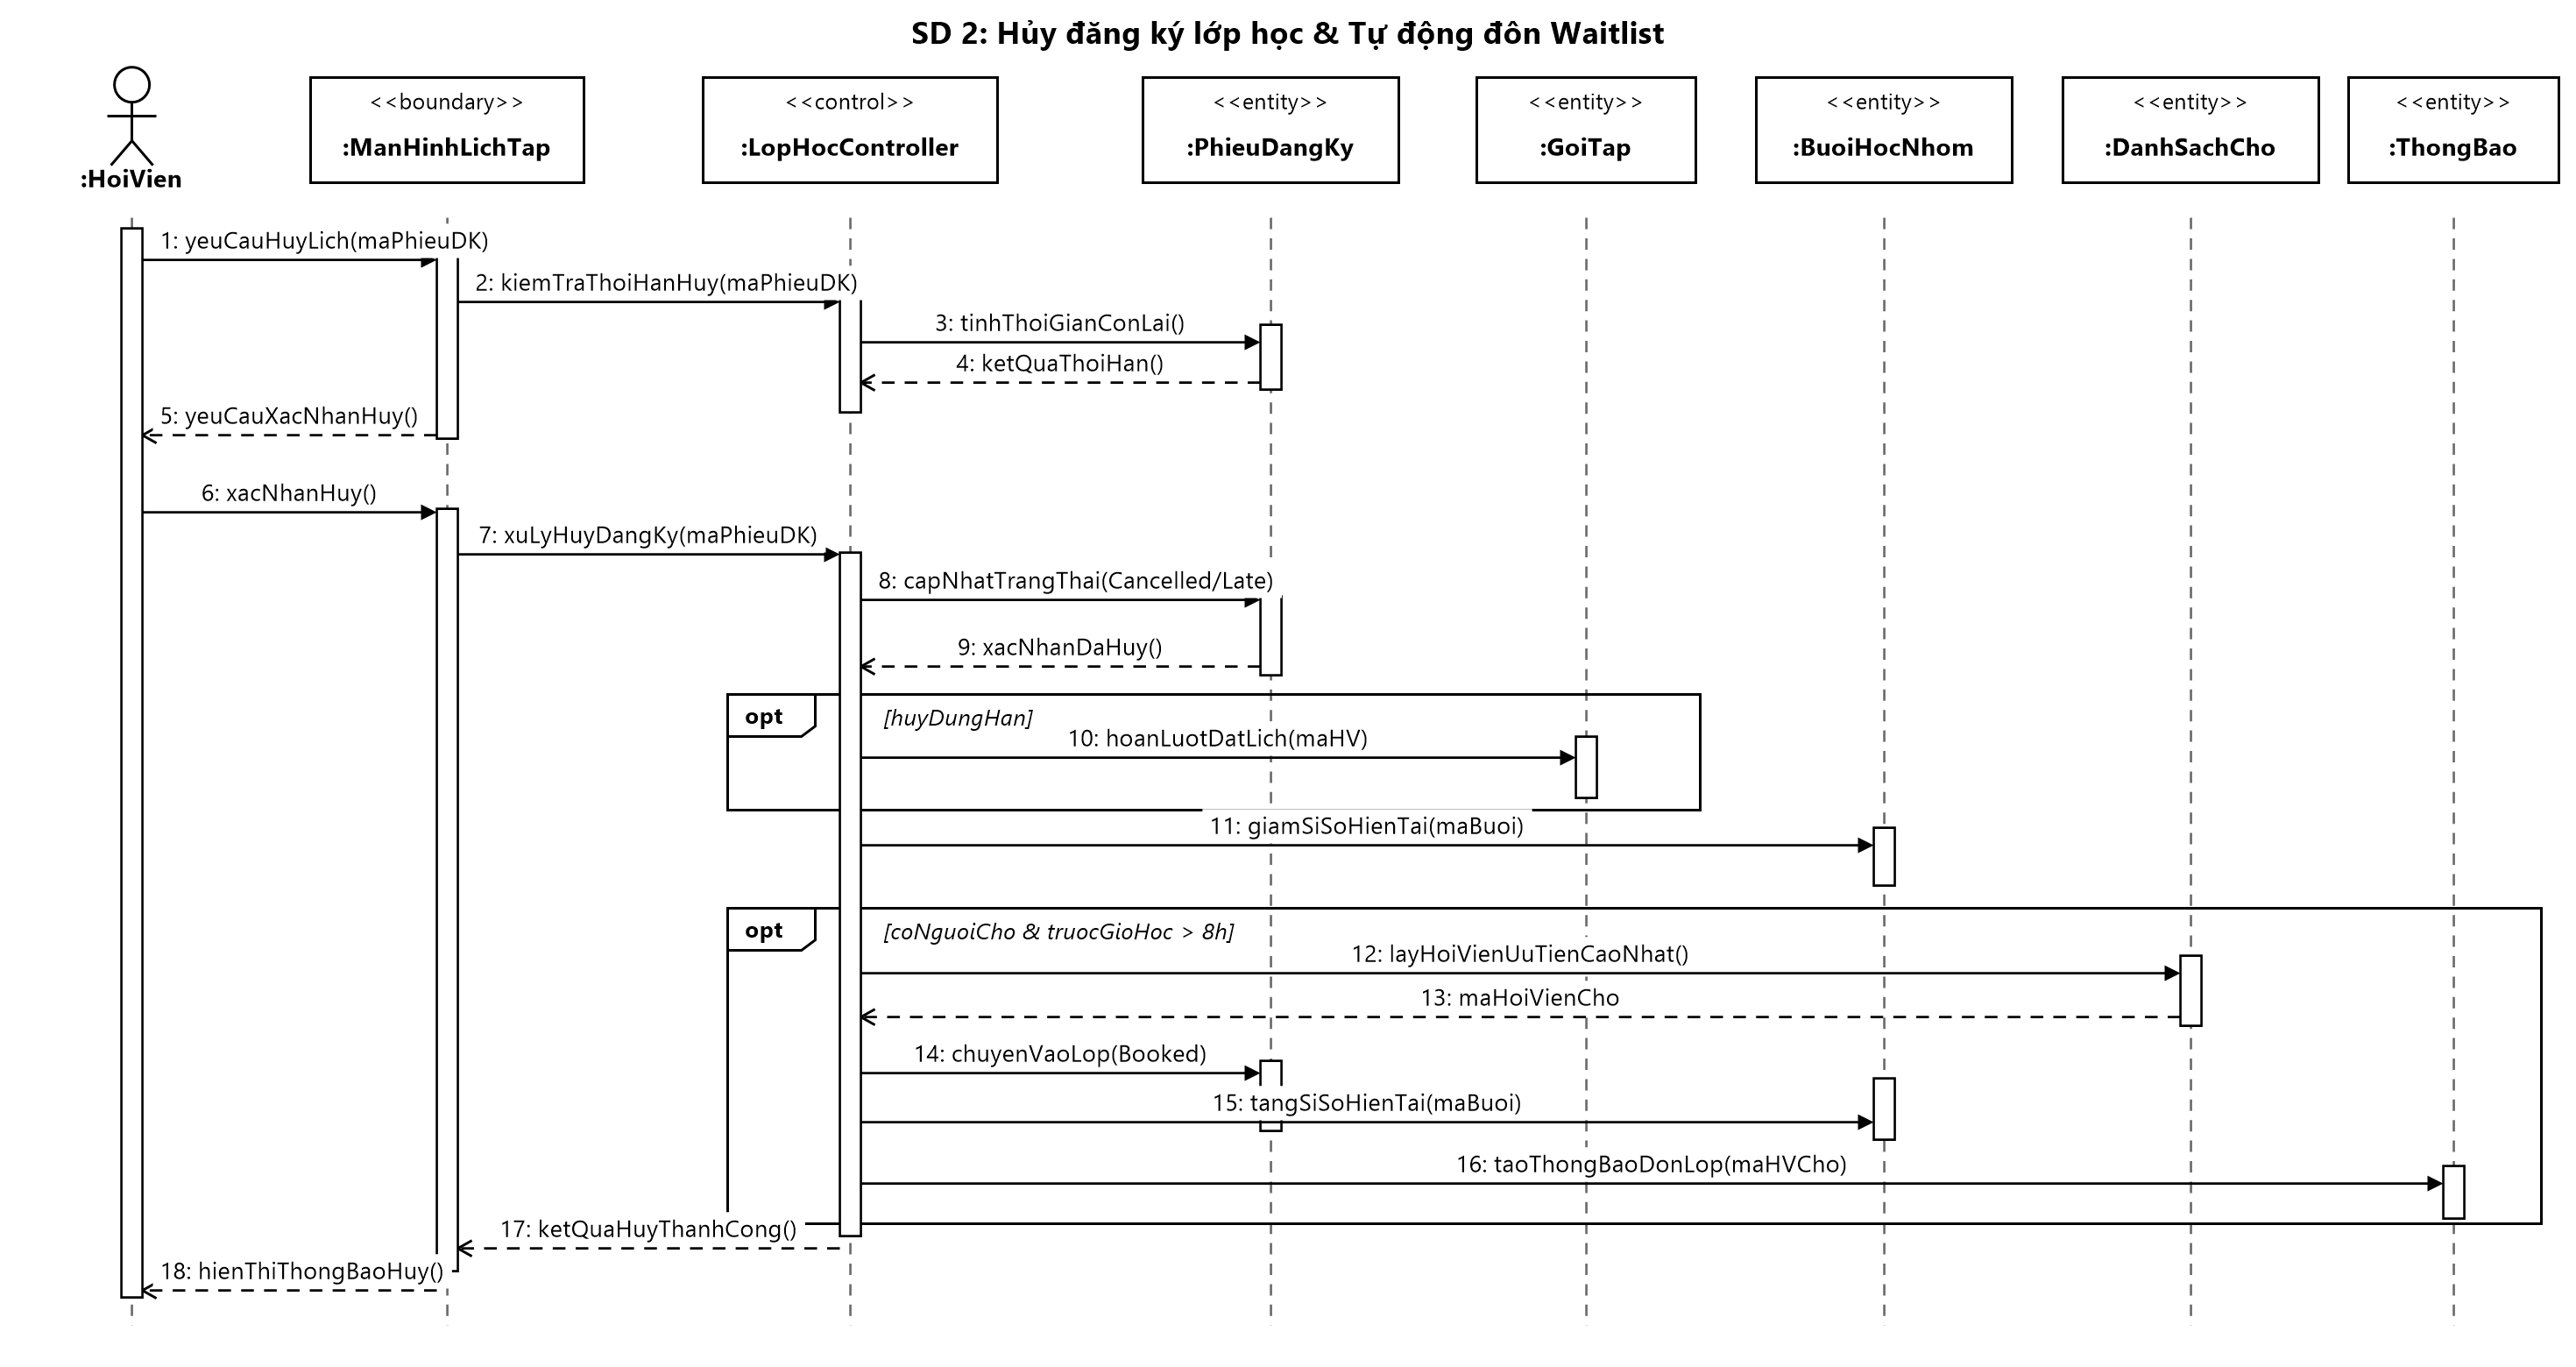
\includegraphics[width=0.95\textwidth, height=0.78\textheight, keepaspectratio]{images/sd_p50_2.png}
\caption{Sequence Diagram 2: Hủy đăng ký lớp học và Tự động đôn người từ Waitlist}
\end{figure}

\begin{figure}[H]
\centering
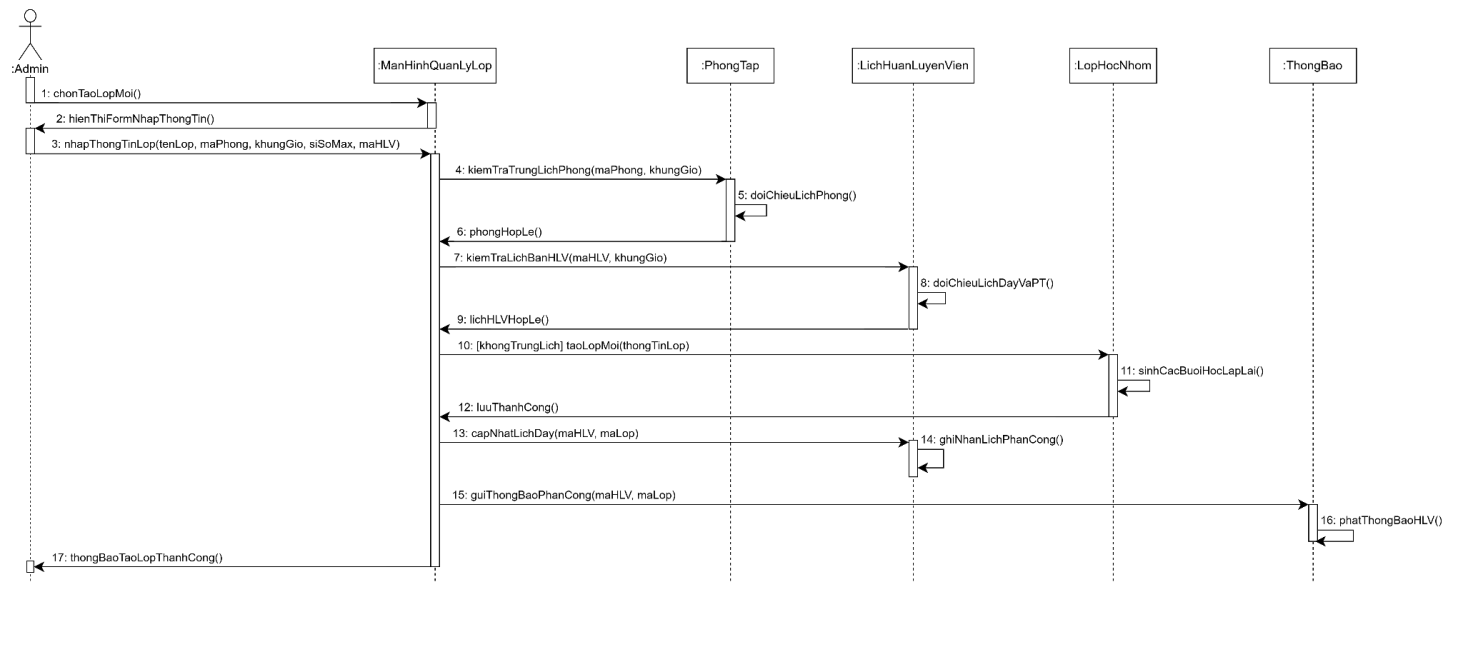
\includegraphics[width=0.95\textwidth, height=0.78\textheight, keepaspectratio]{images/sd_p51_1.png}
\caption{Sequence Diagram 3: Quản lý lớp học nhóm (Tạo lớp \& Phân công HLV)}
\end{figure}

\begin{figure}[H]
\centering
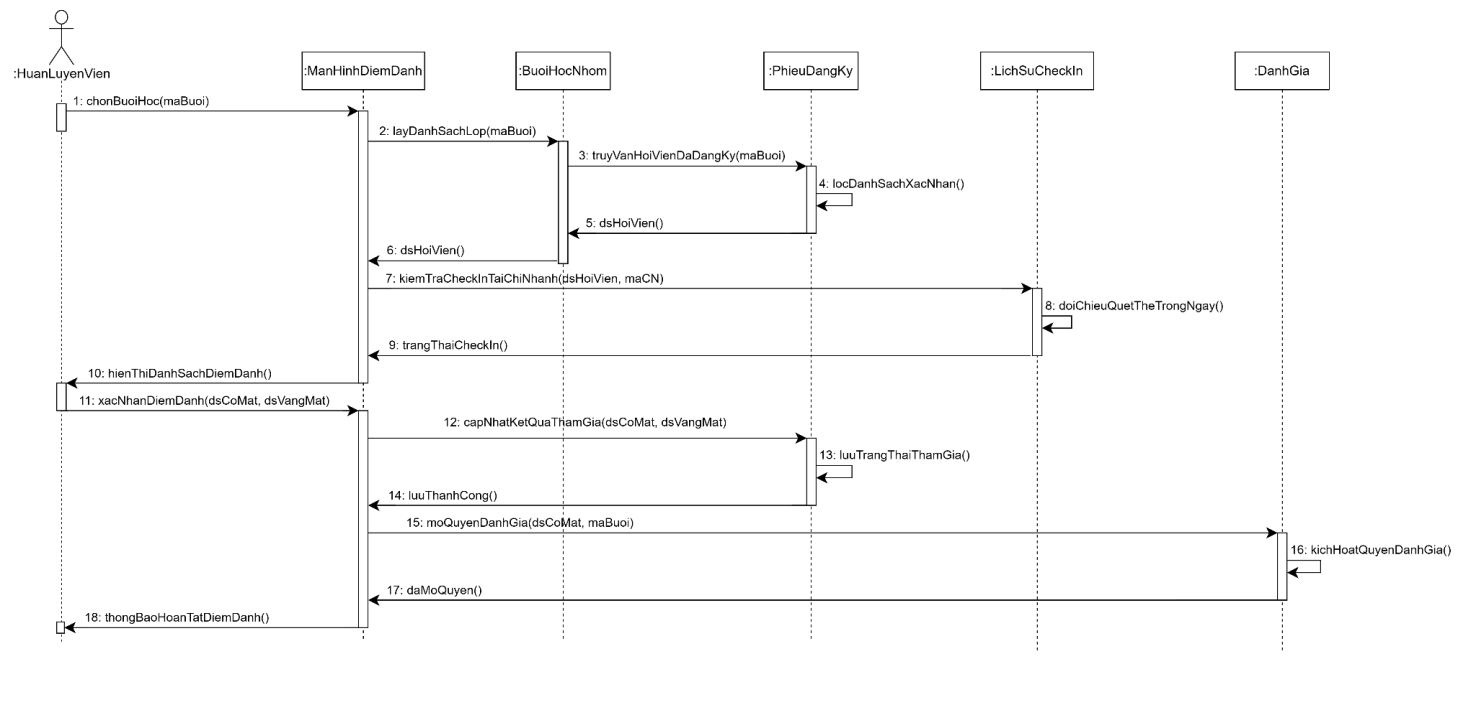
\includegraphics[width=0.95\textwidth, height=0.78\textheight, keepaspectratio]{images/sd_p51_2.png}
\caption{Sequence Diagram 4: Điểm danh lớp học nhóm}
\end{figure}

\subsubsection{Nhóm luồng Đặt lịch PT 1-kèm-1 \& Lịch rảnh}

\begin{figure}[H]
\centering
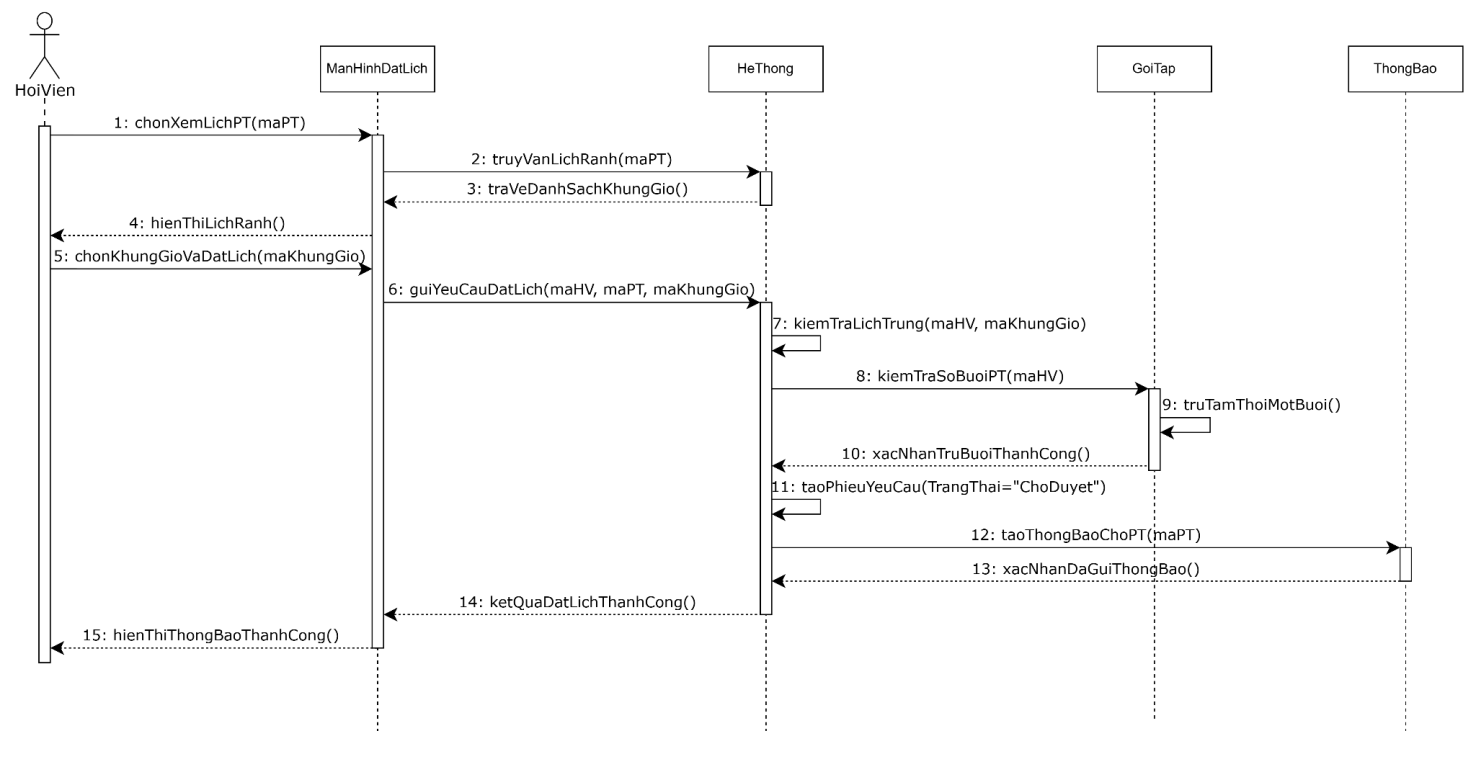
\includegraphics[width=0.95\textwidth, height=0.78\textheight, keepaspectratio]{images/sd_p52_1.png}
\caption{Sequence Diagram 5: Đặt lịch lớp PT}
\end{figure}

\begin{figure}[H]
\centering
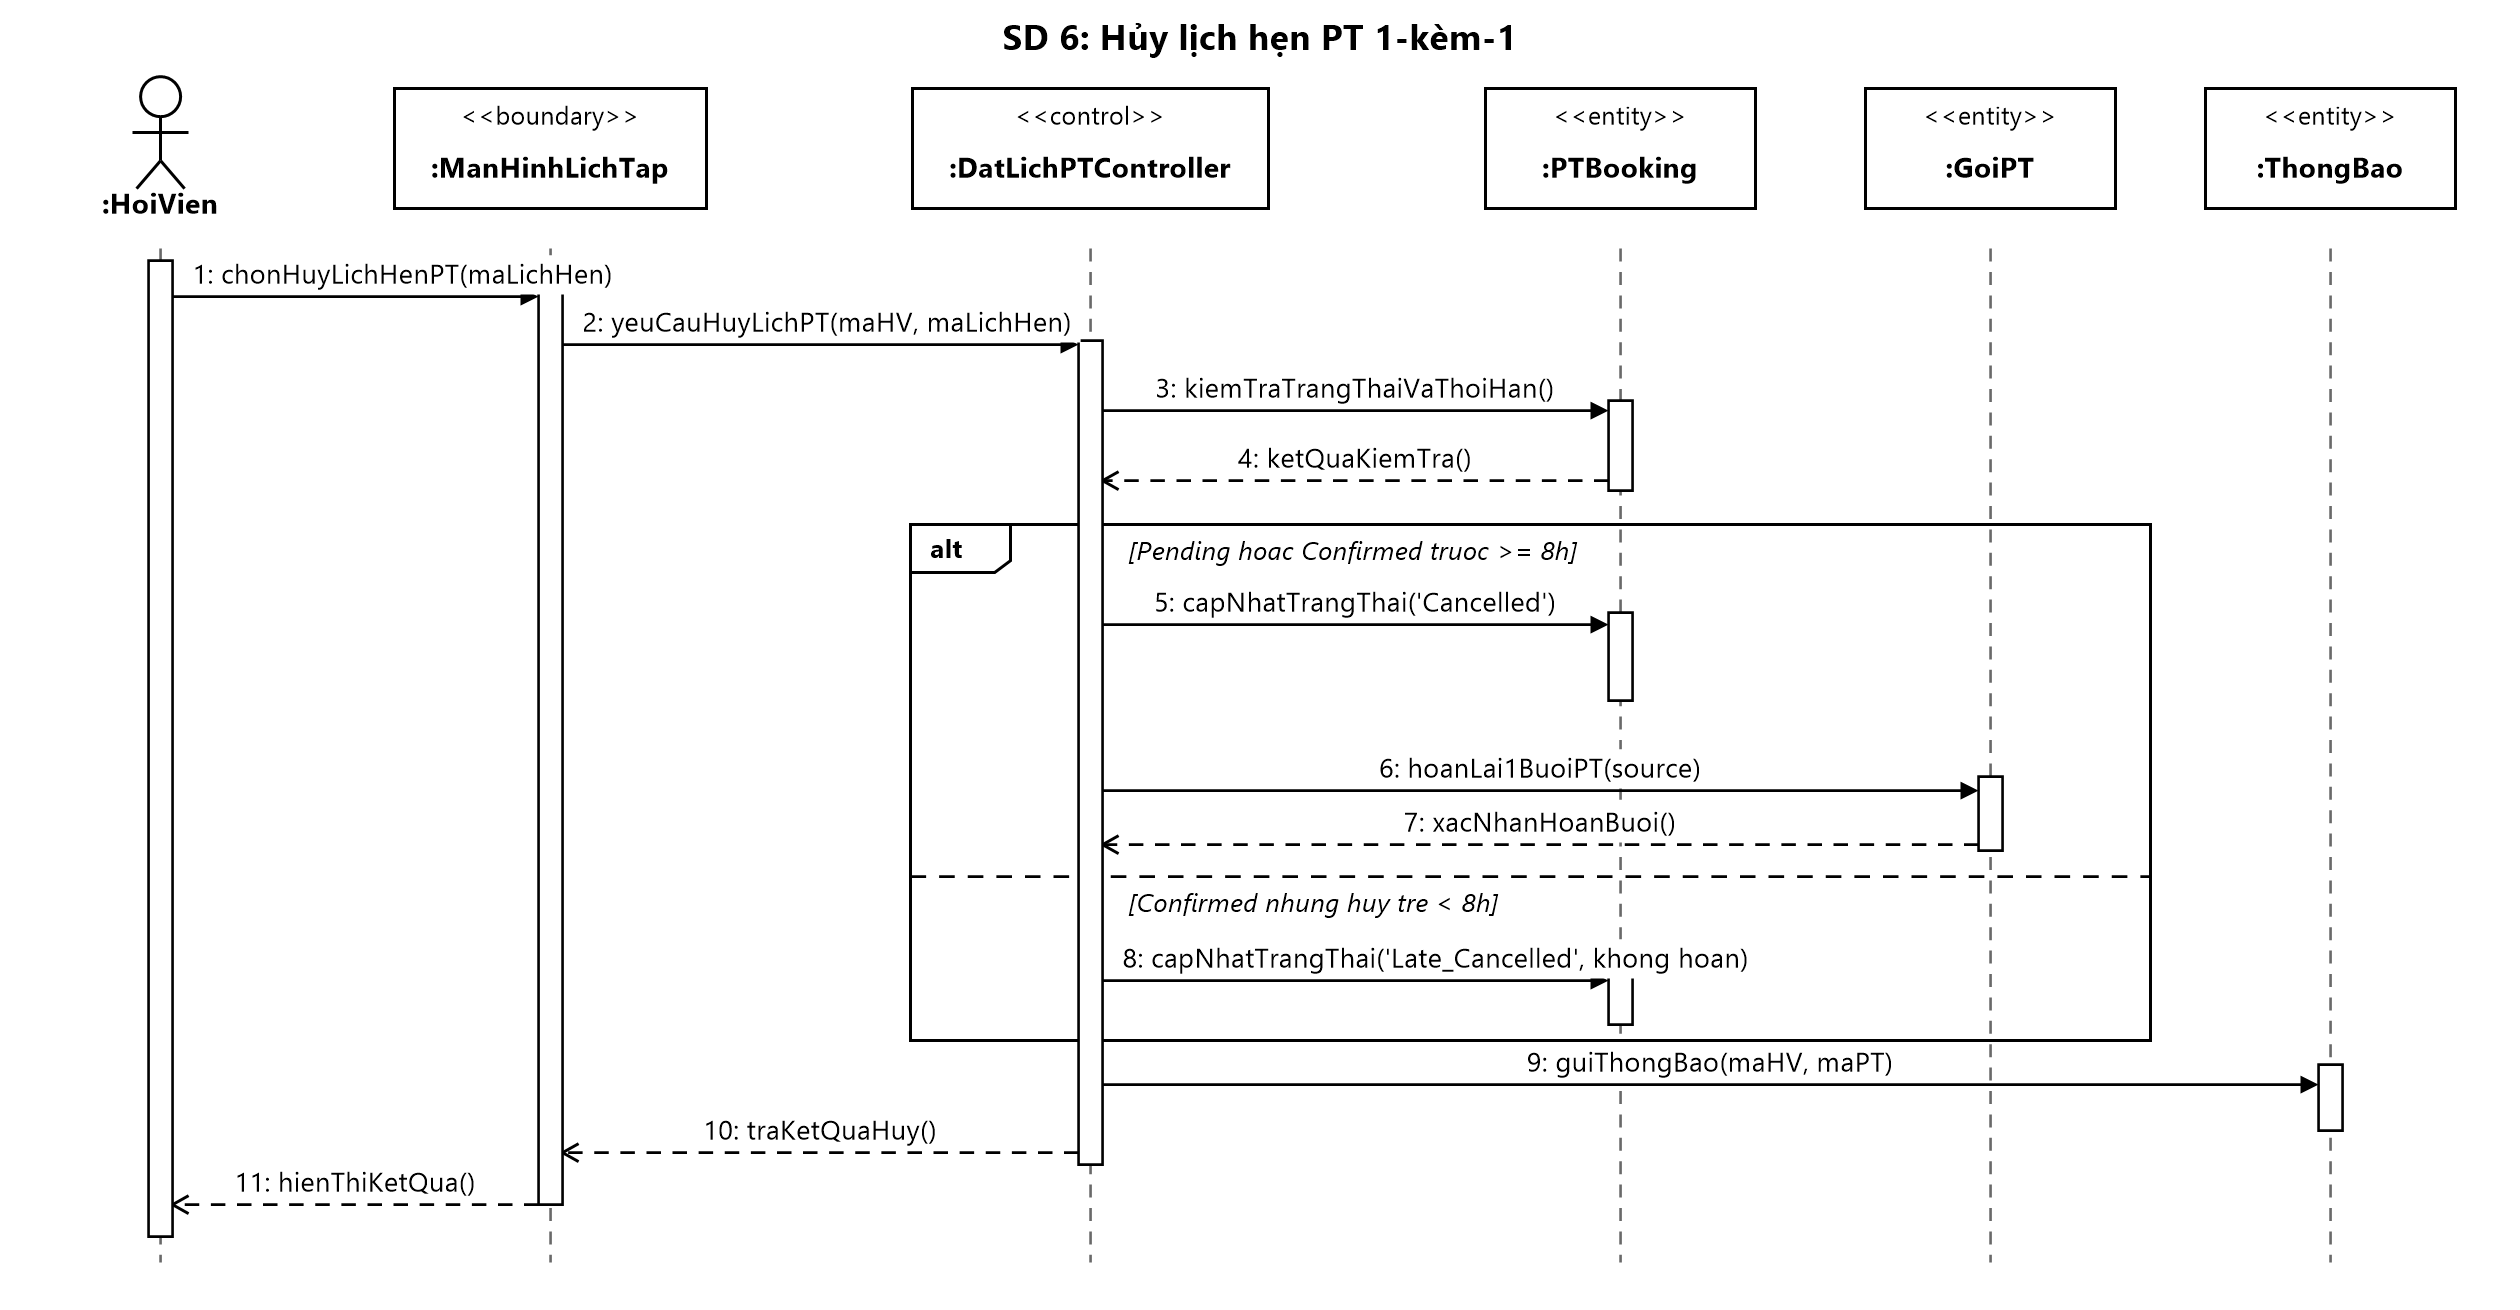
\includegraphics[width=0.95\textwidth, height=0.78\textheight, keepaspectratio]{images/sd_p52_2.png}
\caption{Sequence Diagram 6: Hủy lịch lớp PT}
\end{figure}

\begin{figure}[H]
\centering
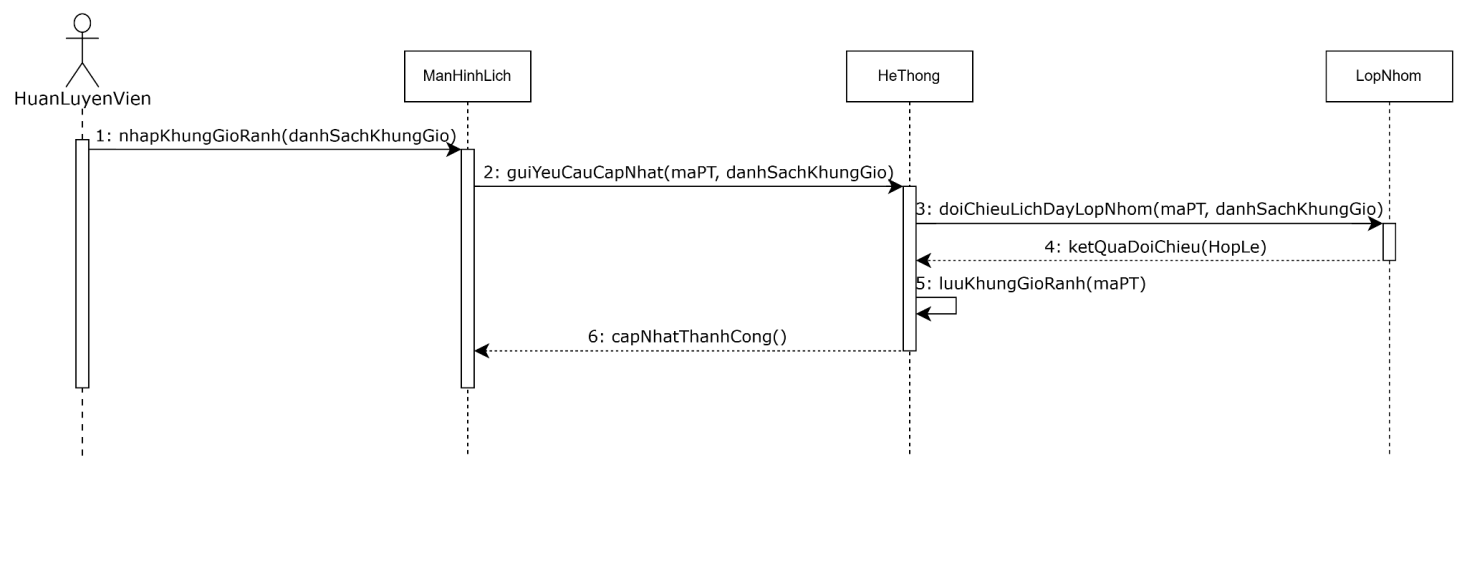
\includegraphics[width=0.95\textwidth, height=0.78\textheight, keepaspectratio]{images/sd_p53_1.png}
\caption{Sequence Diagram 7: Cập nhật khung giờ rảnh của PT}
\end{figure}

\begin{figure}[H]
\centering
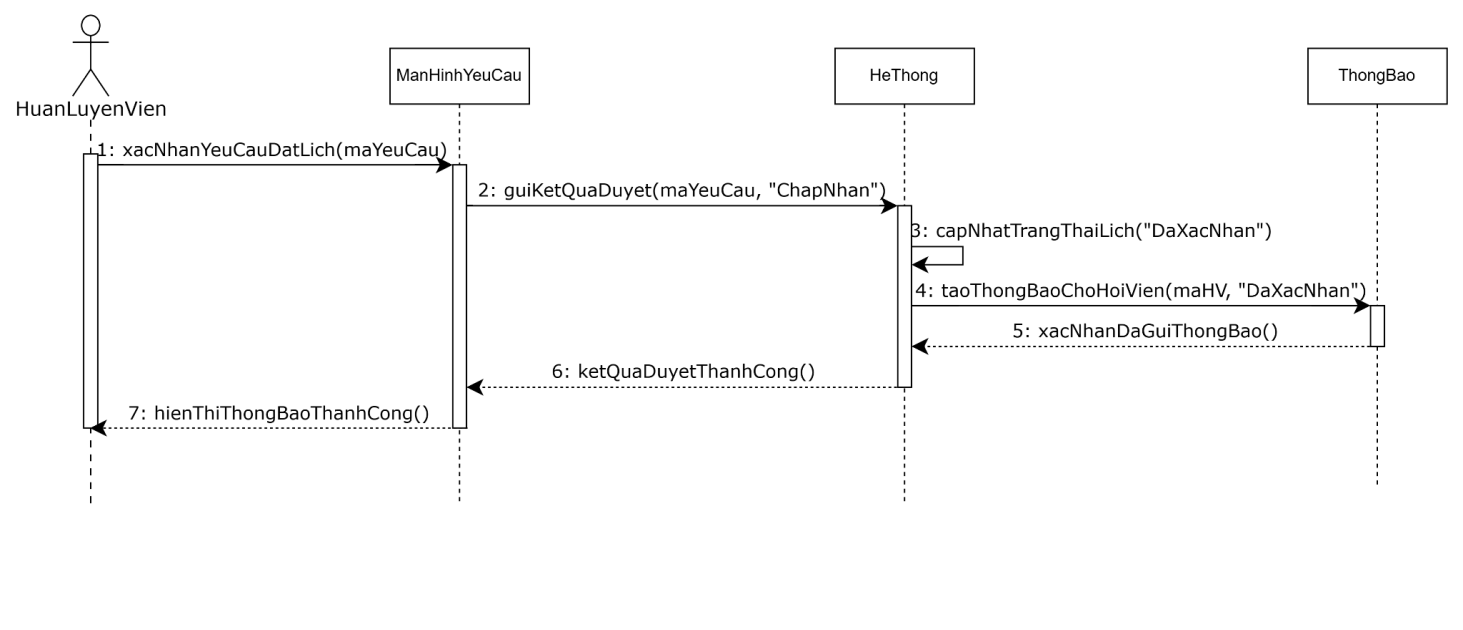
\includegraphics[width=0.95\textwidth, height=0.78\textheight, keepaspectratio]{images/sd_p53_2.png}
\caption{Sequence Diagram 8: Xác nhận yêu cầu đặt lịch}
\end{figure}

\subsubsection{Nhóm luồng Check-in, Tiến độ, Báo cáo \& Thông báo}

\begin{figure}[H]
\centering
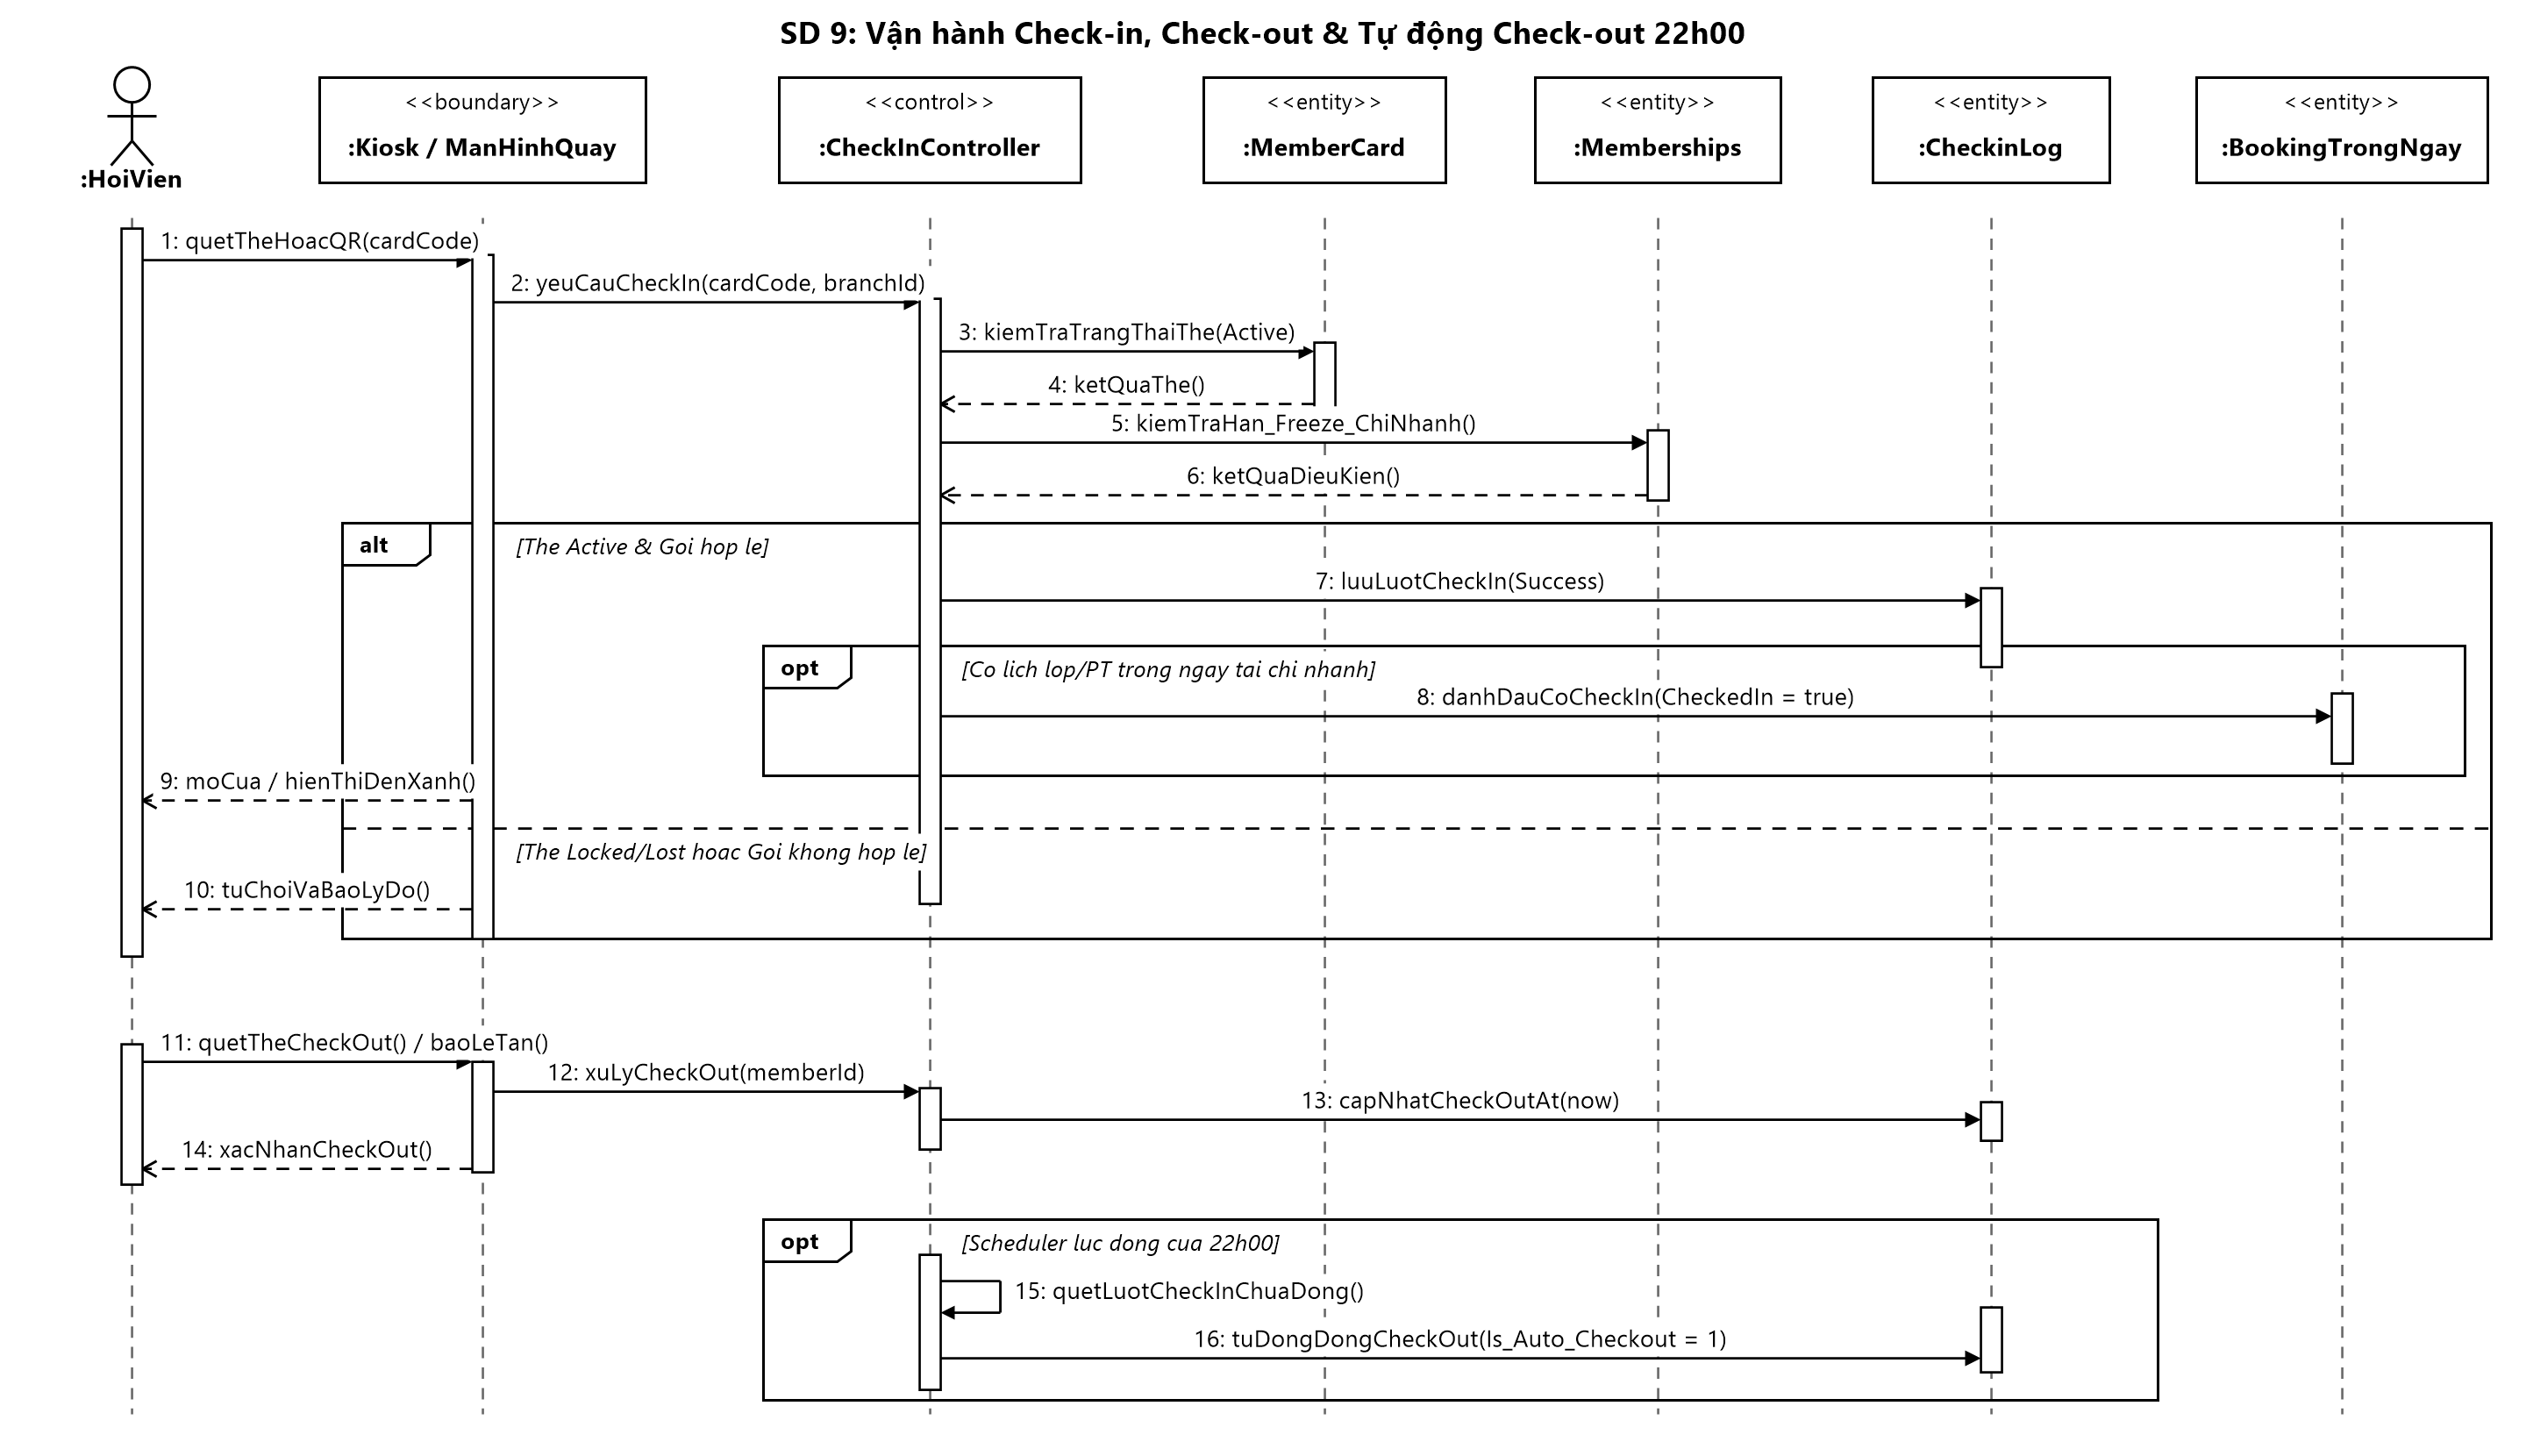
\includegraphics[width=0.95\textwidth, height=0.78\textheight, keepaspectratio]{images/sd_p54_1.png}
\caption{Sequence Diagram 9: Check-in và Check-out}
\end{figure}

\begin{figure}[H]
\centering
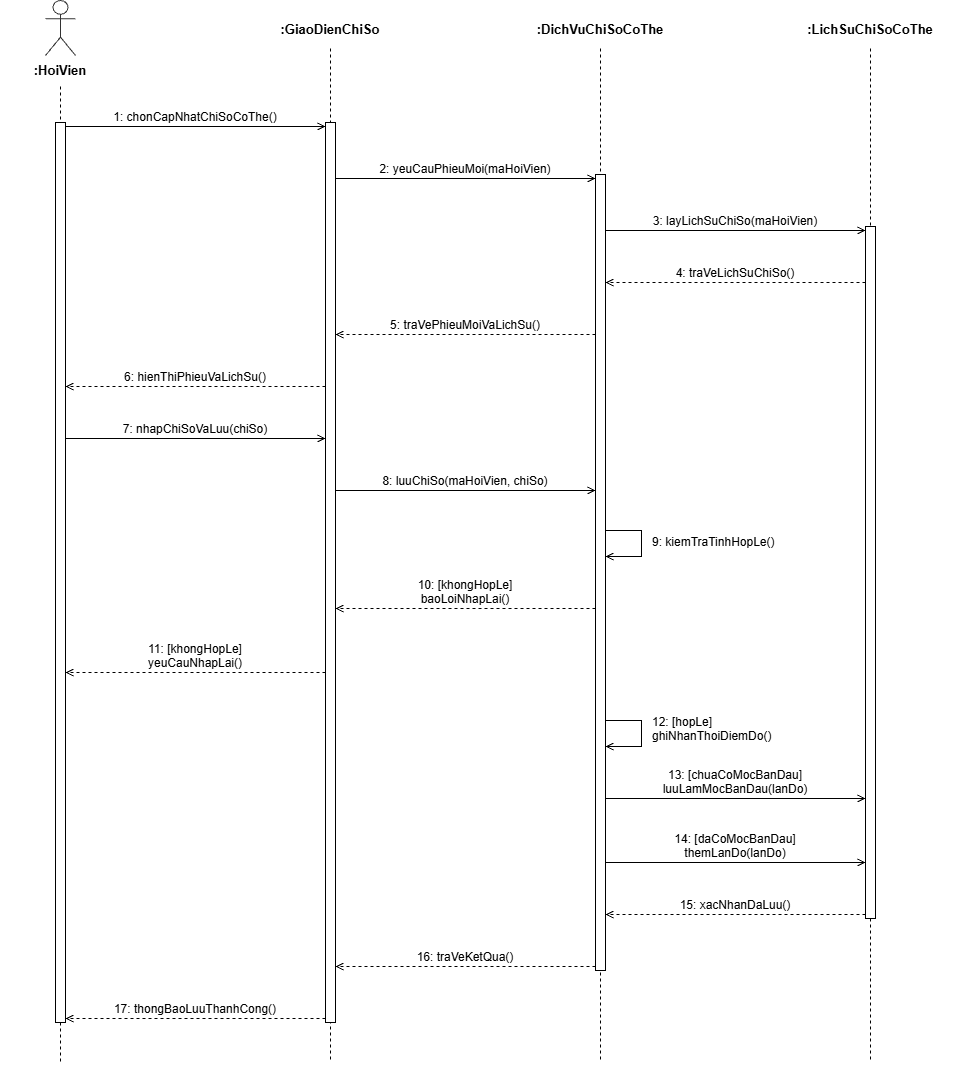
\includegraphics[width=0.95\textwidth, height=0.78\textheight, keepaspectratio]{images/sd_p55_1.png}
\caption{Sequence Diagram 10: Cập nhật tiến độ chỉ số cơ thể}
\end{figure}

\begin{figure}[H]
\centering
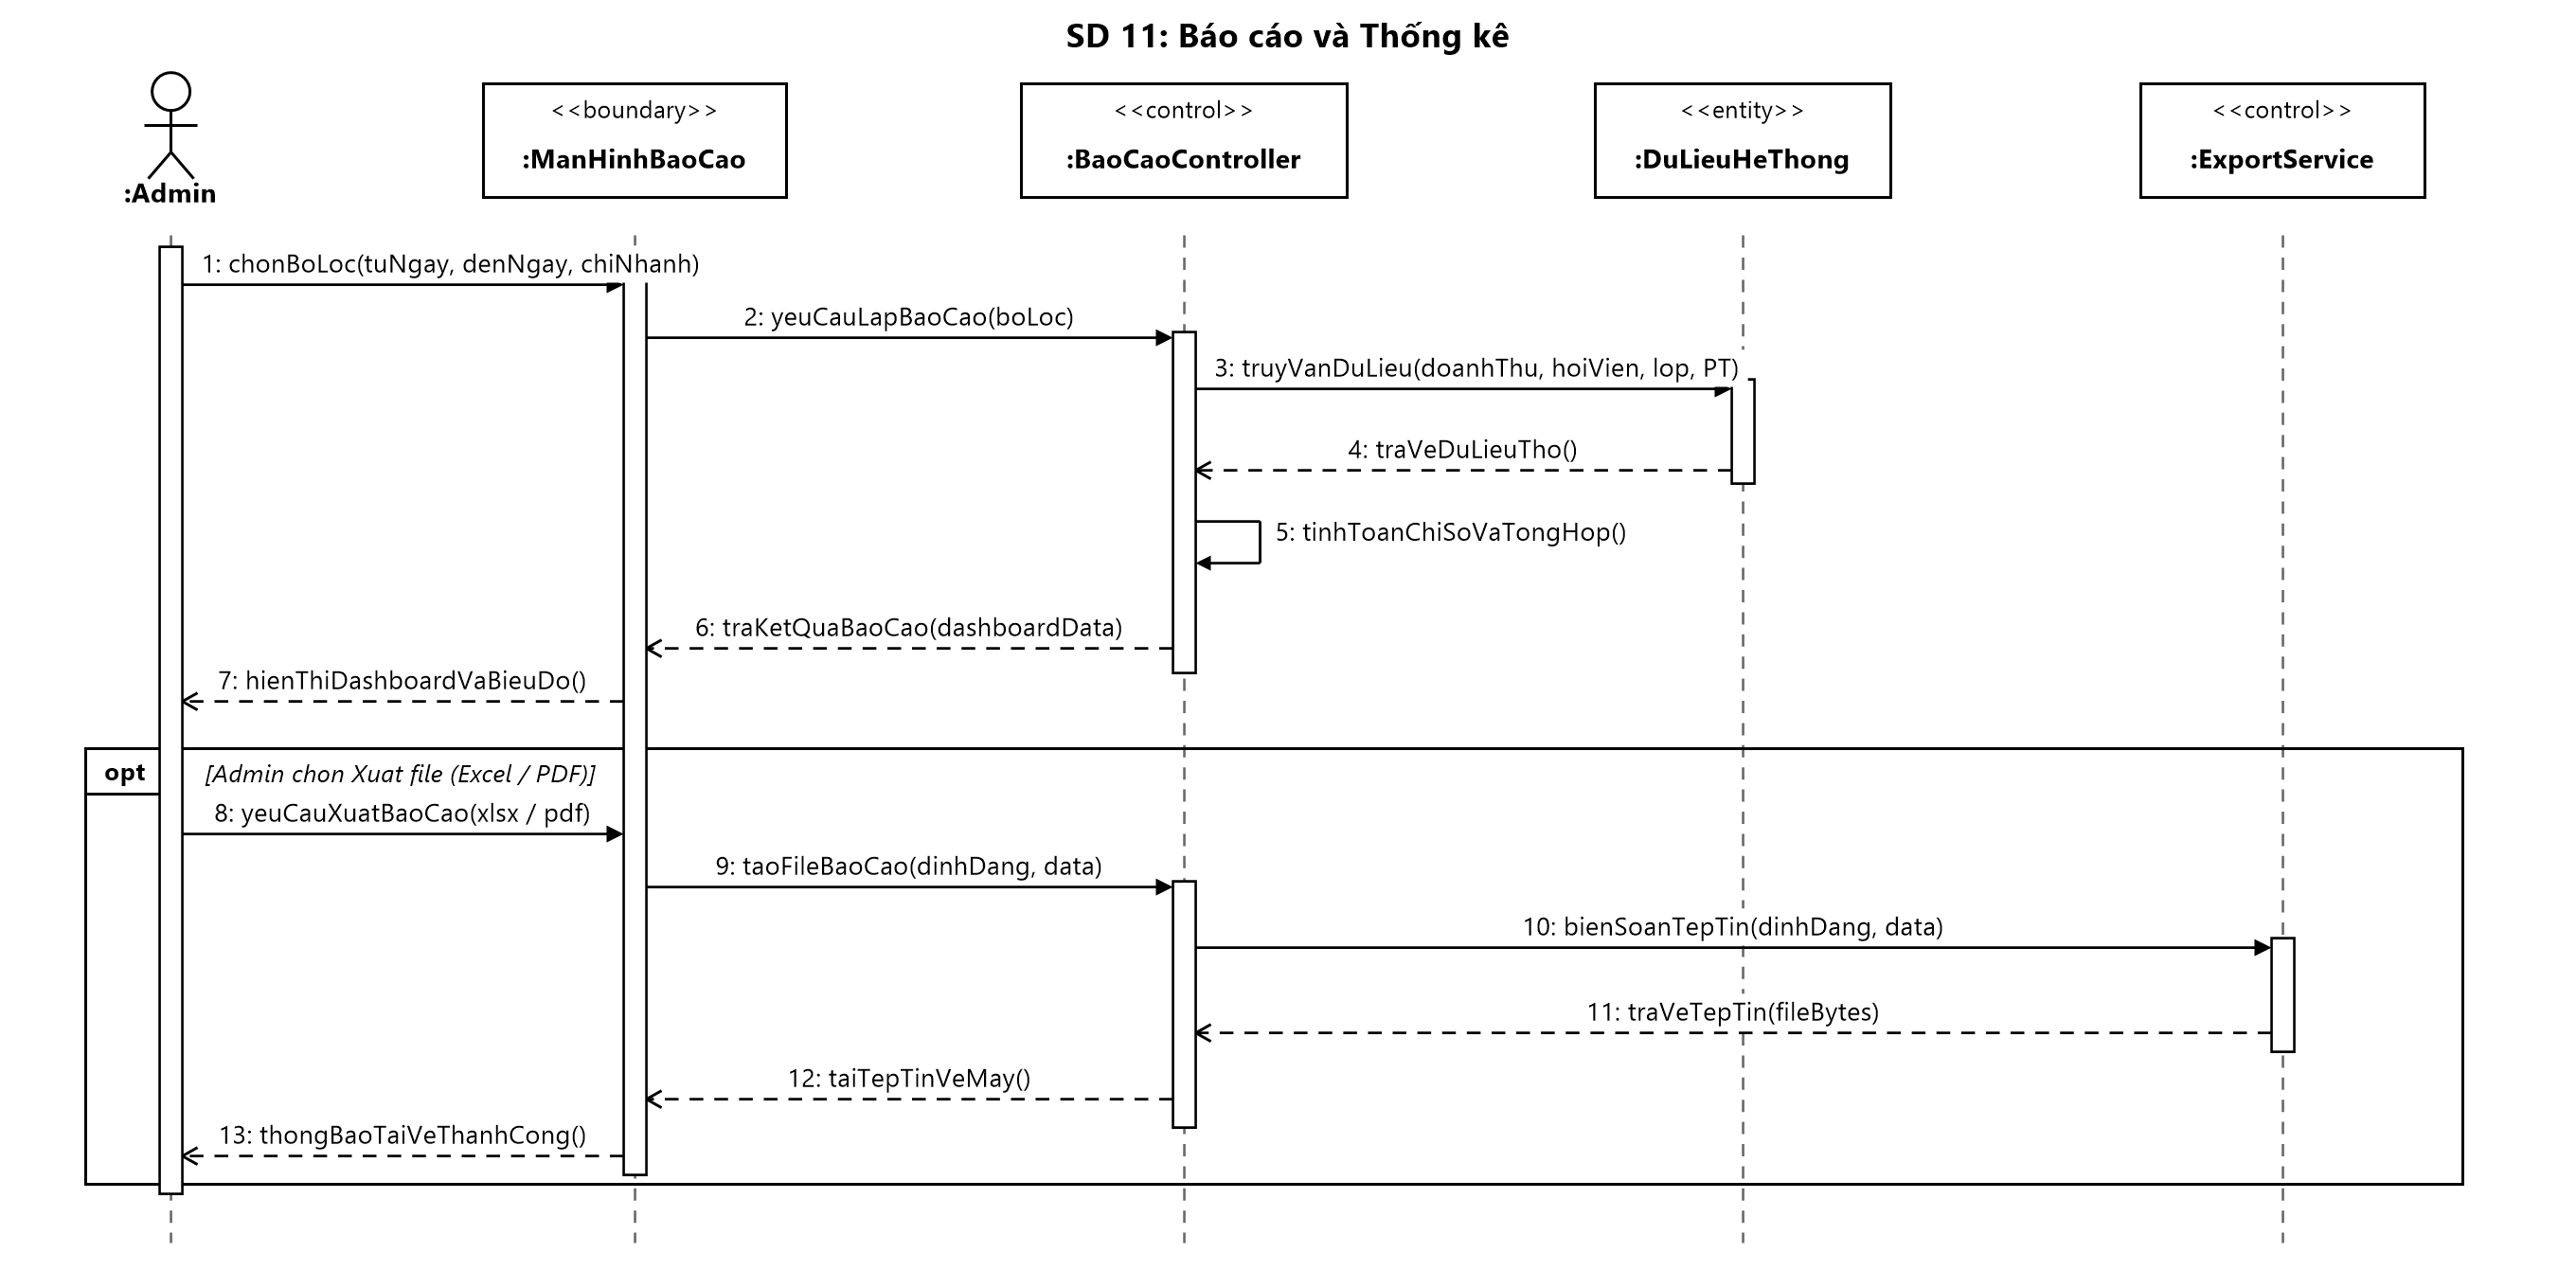
\includegraphics[width=0.95\textwidth, height=0.78\textheight, keepaspectratio]{images/sd_p56_1.png}
\caption{Sequence Diagram 11: Báo cáo và Thống kê}
\end{figure}

\begin{figure}[H]
\centering
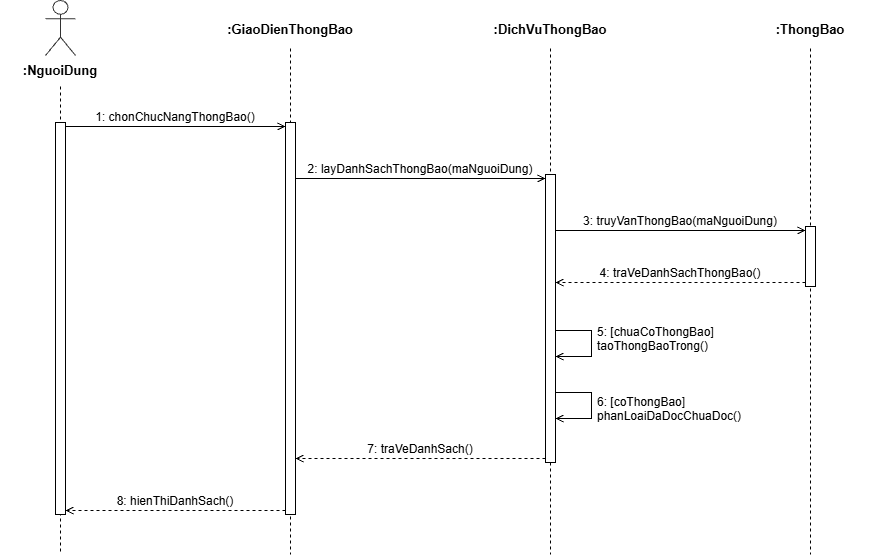
\includegraphics[width=0.95\textwidth, height=0.78\textheight, keepaspectratio]{images/sd_p57_1.png}
\caption{Sequence Diagram 12: Xem thông báo}
\end{figure}

\begin{figure}[H]
\centering
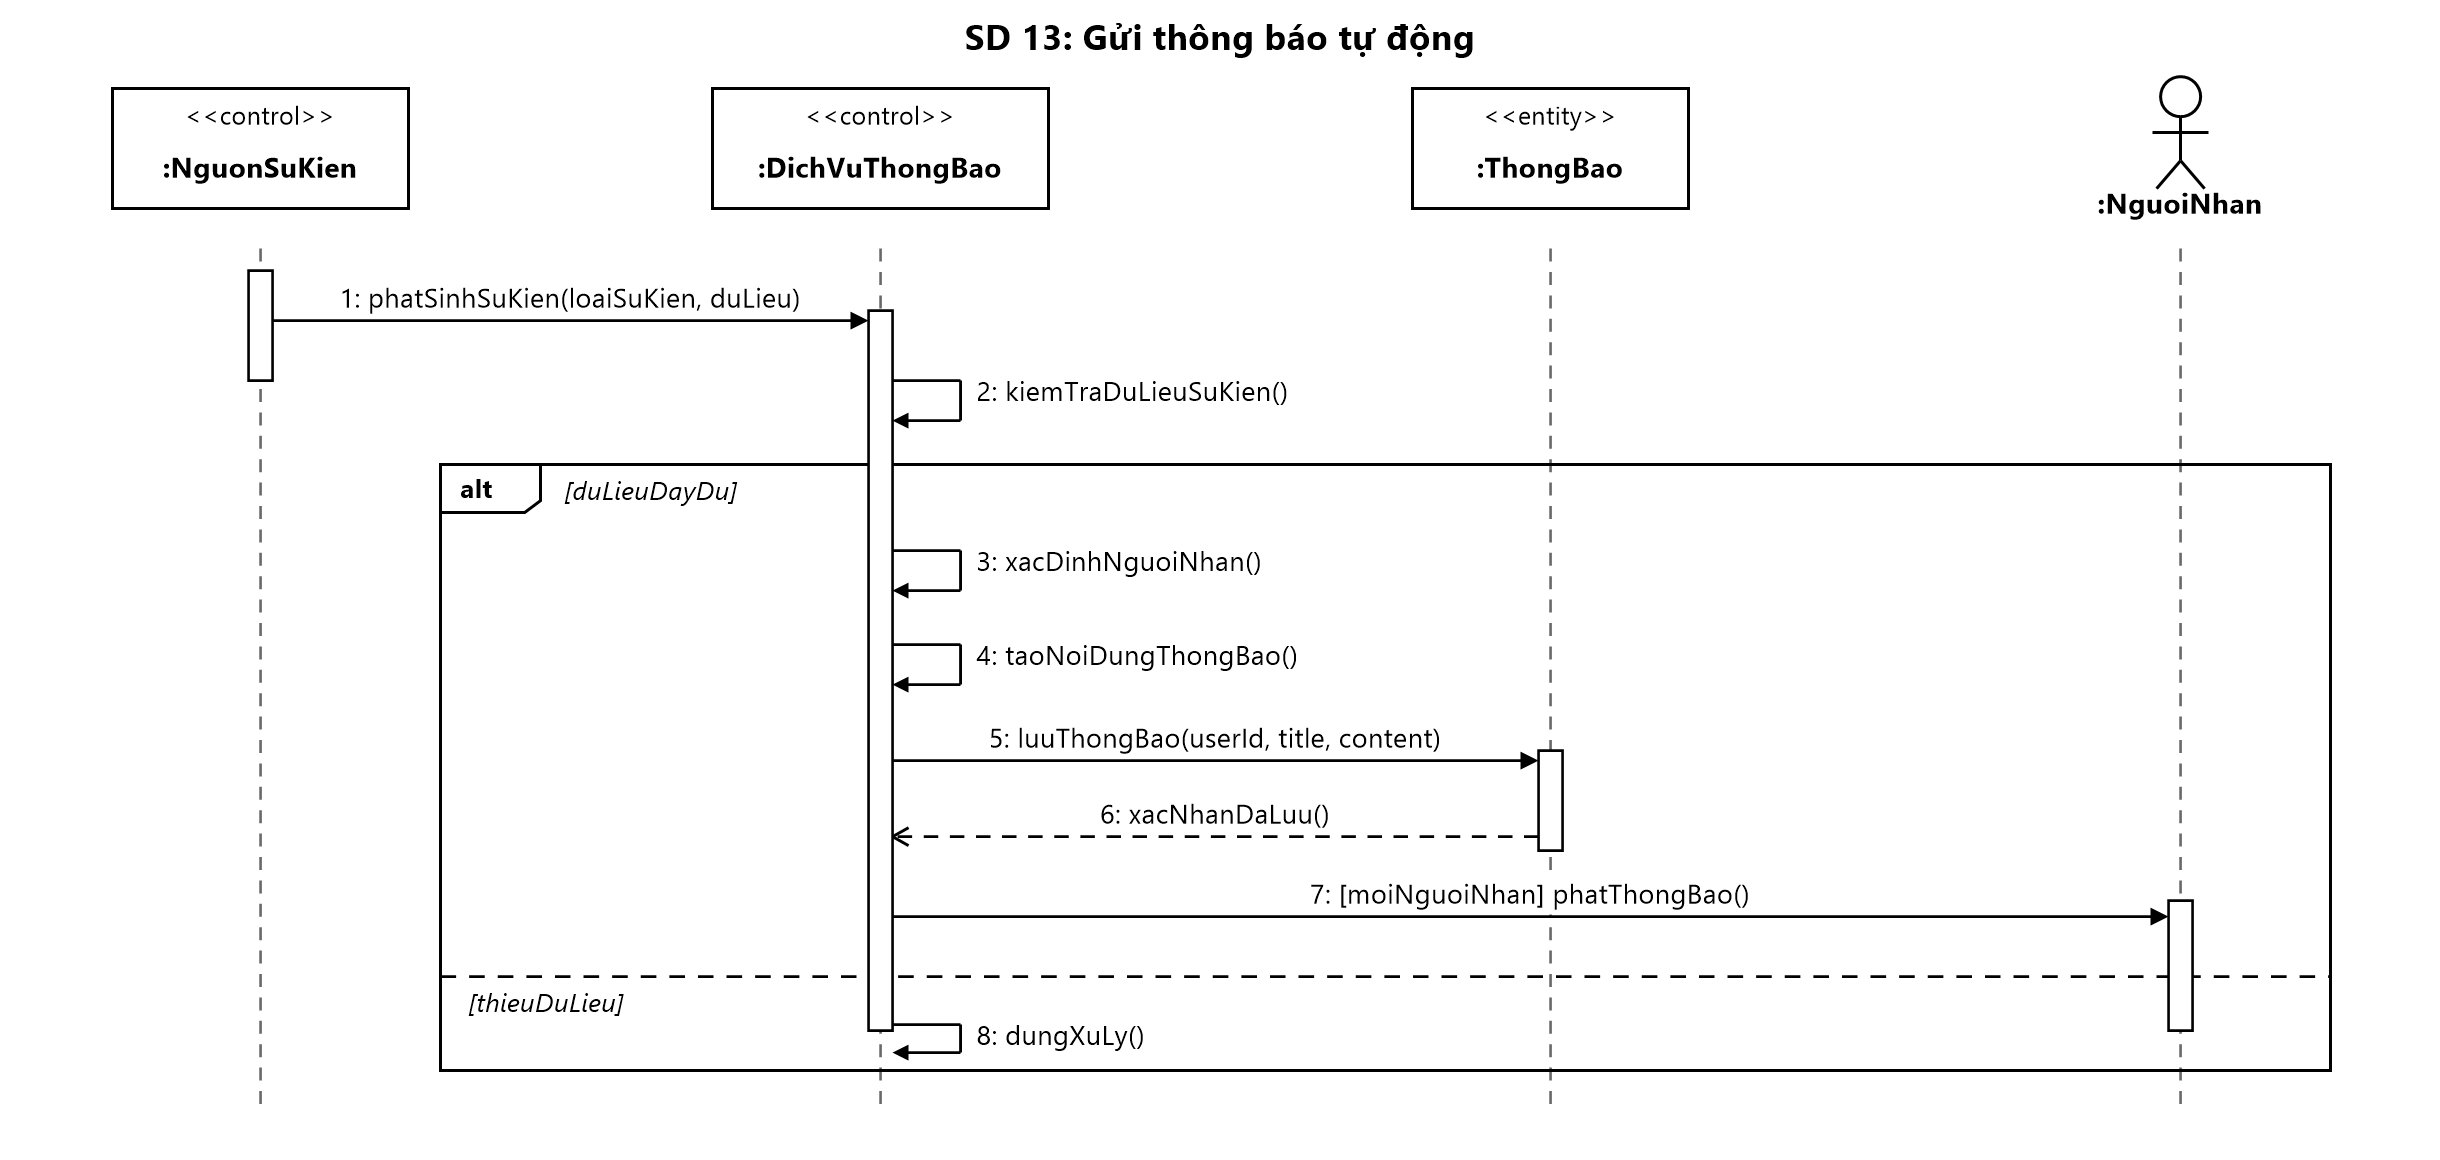
\includegraphics[width=0.95\textwidth, height=0.78\textheight, keepaspectratio]{images/sd_p58_1.png}
\caption{Sequence Diagram 13: Gửi thông báo tự động}
\end{figure}

\subsubsection{Nhóm luồng Gói tập \& Thanh toán Online}

\begin{figure}[H]
\centering
\includegraphics[page=59, width=0.95\textwidth, trim=2.2cm 14.8cm 1.5cm 2.4cm, clip]{UC-Sequence_NhomBaKhi.pdf}
\caption{Sequence Diagram 14: Thanh toán Online}
\end{figure}

\begin{figure}[H]
\centering
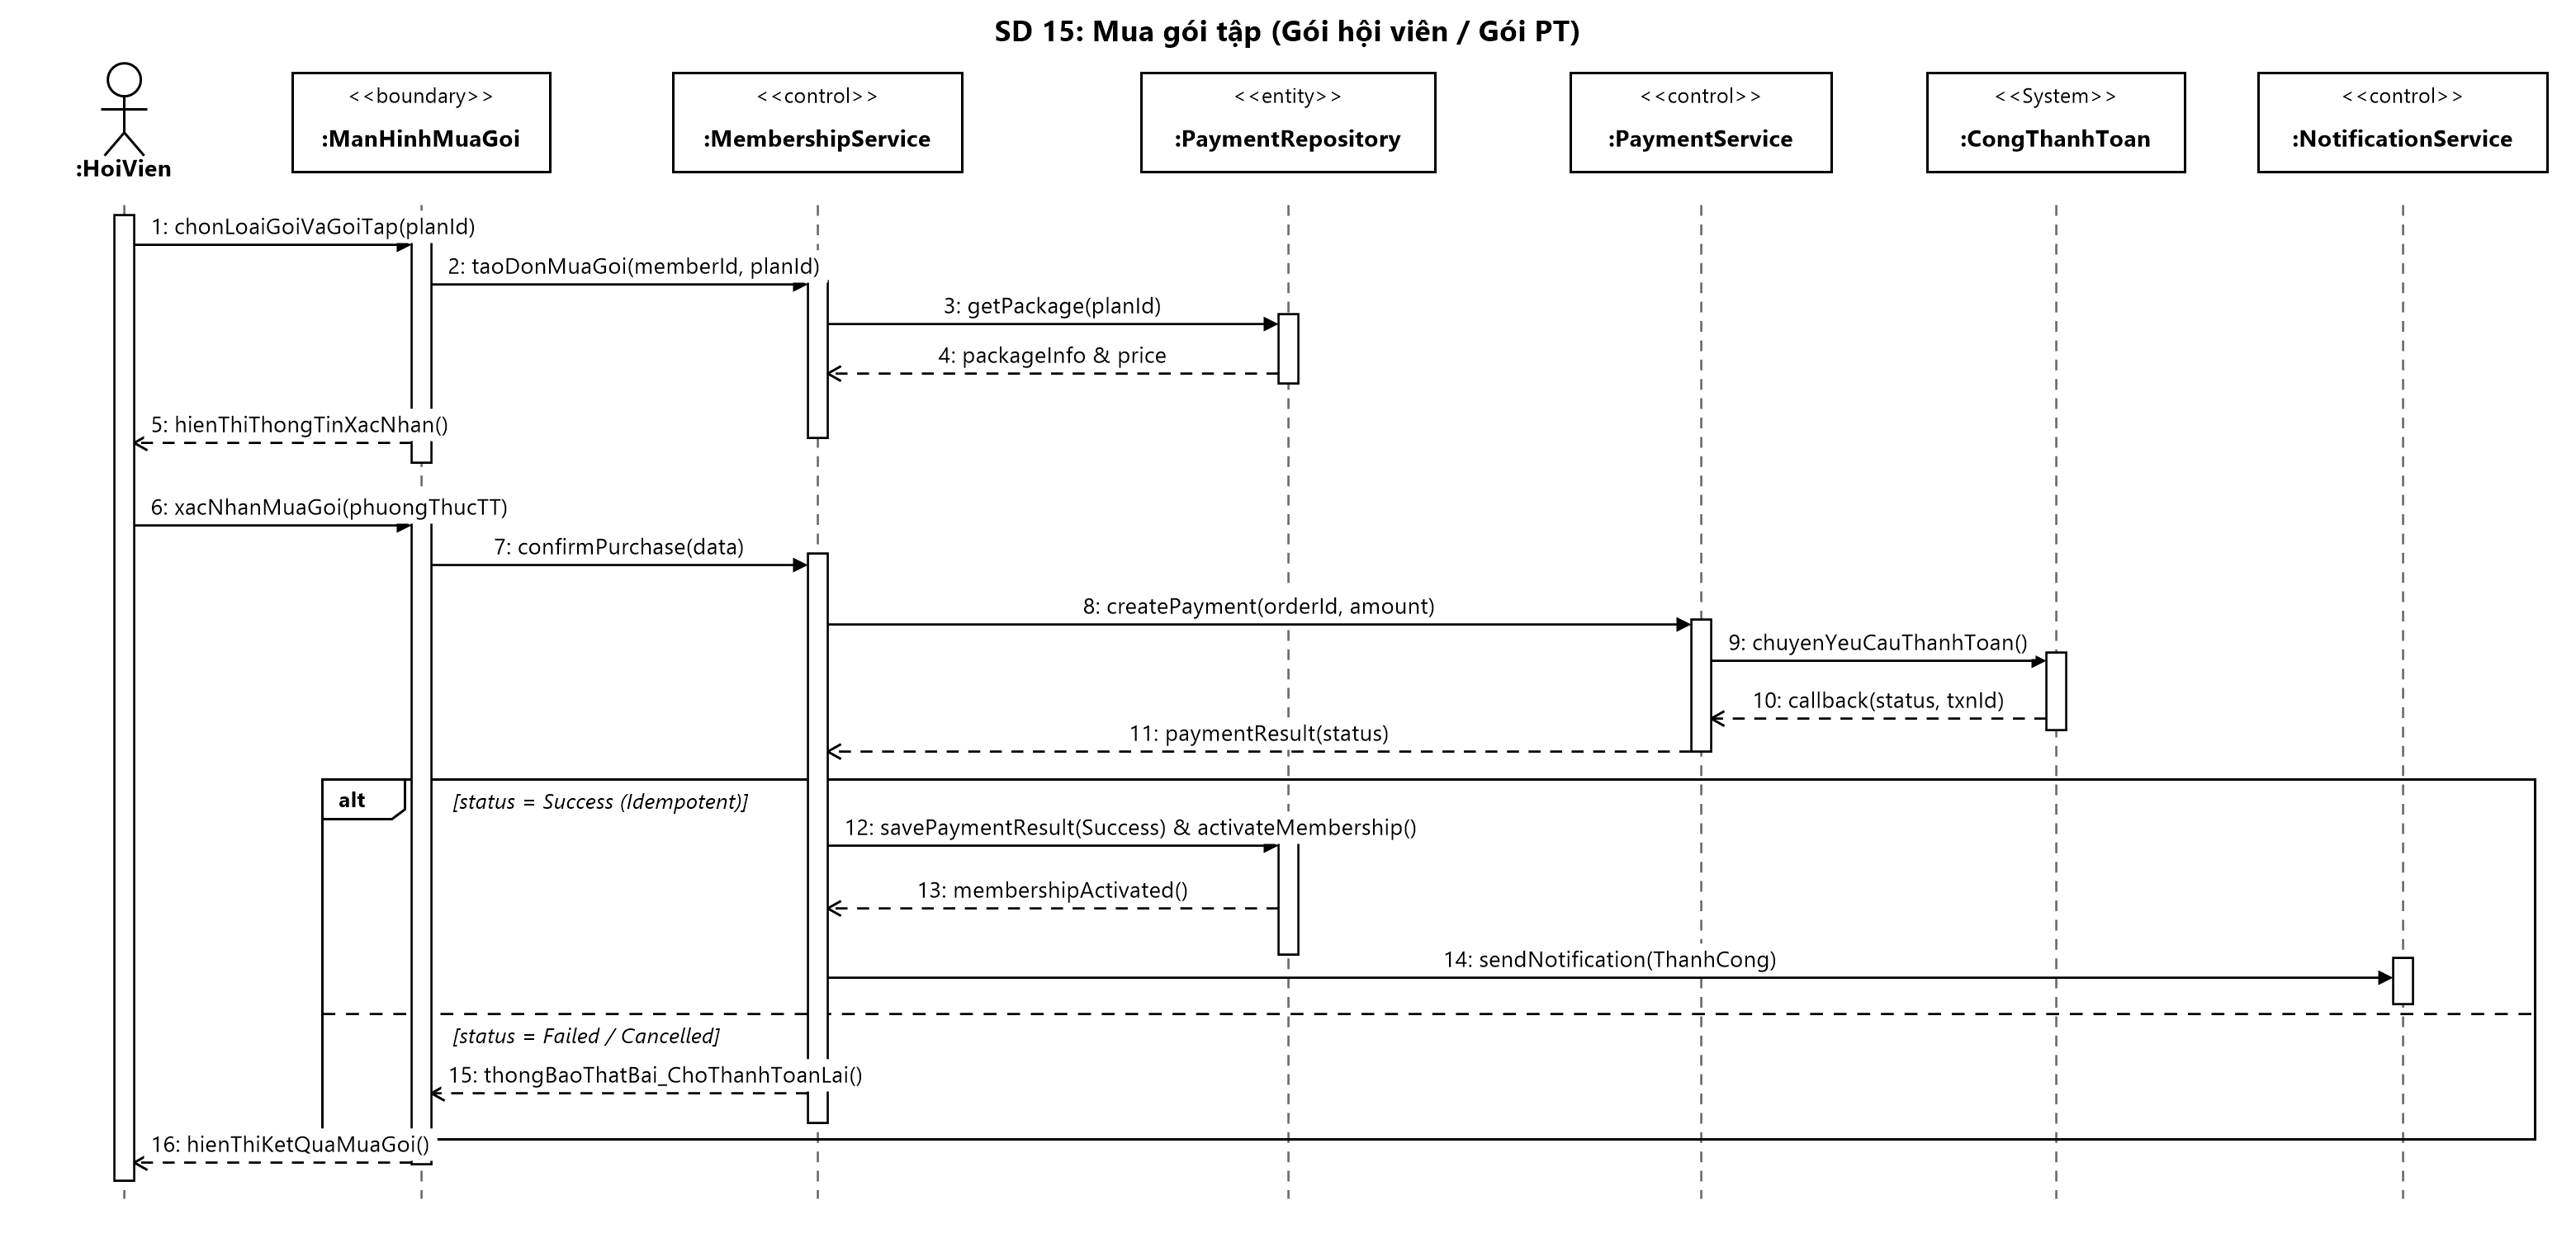
\includegraphics[width=0.95\textwidth, height=0.78\textheight, keepaspectratio]{images/sd_p59_2.png}
\caption{Sequence Diagram 15: Mua gói tập}
\end{figure}

\begin{figure}[H]
\centering
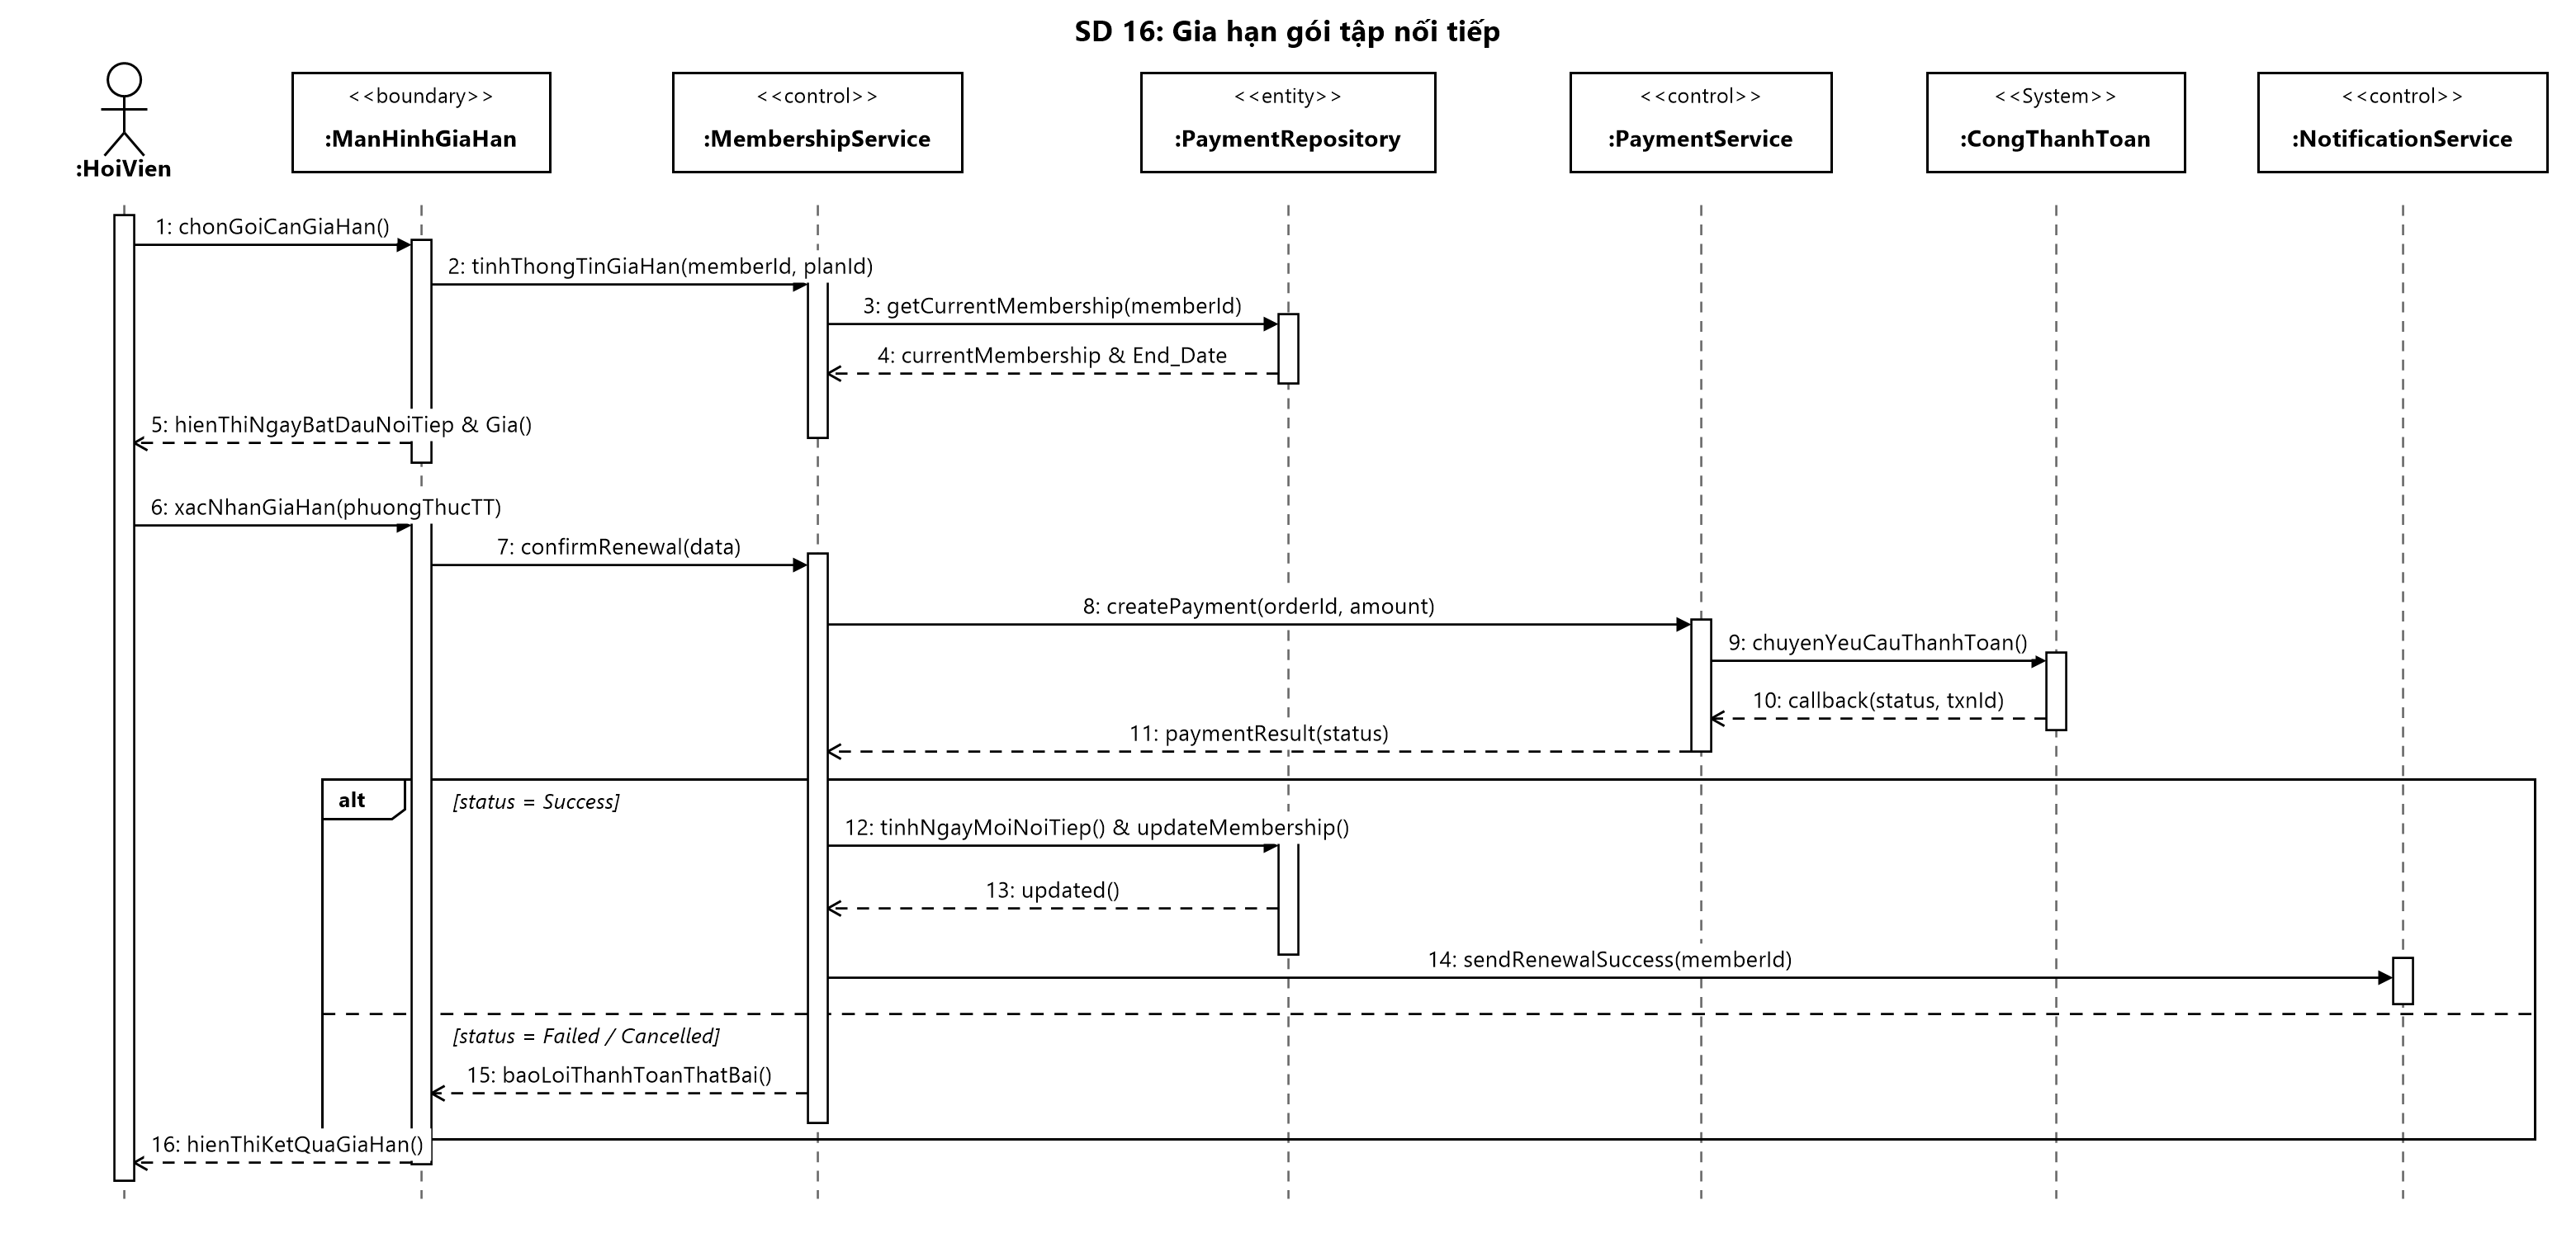
\includegraphics[width=0.95\textwidth, height=0.78\textheight, keepaspectratio]{images/sd_p60_1.png}
\caption{Sequence Diagram 16: Gia hạn gói tập}
\end{figure}

\subsubsection{Nhóm luồng Chi nhánh, Thiết bị \& Xử lý sự cố}

\begin{figure}[H]
\centering
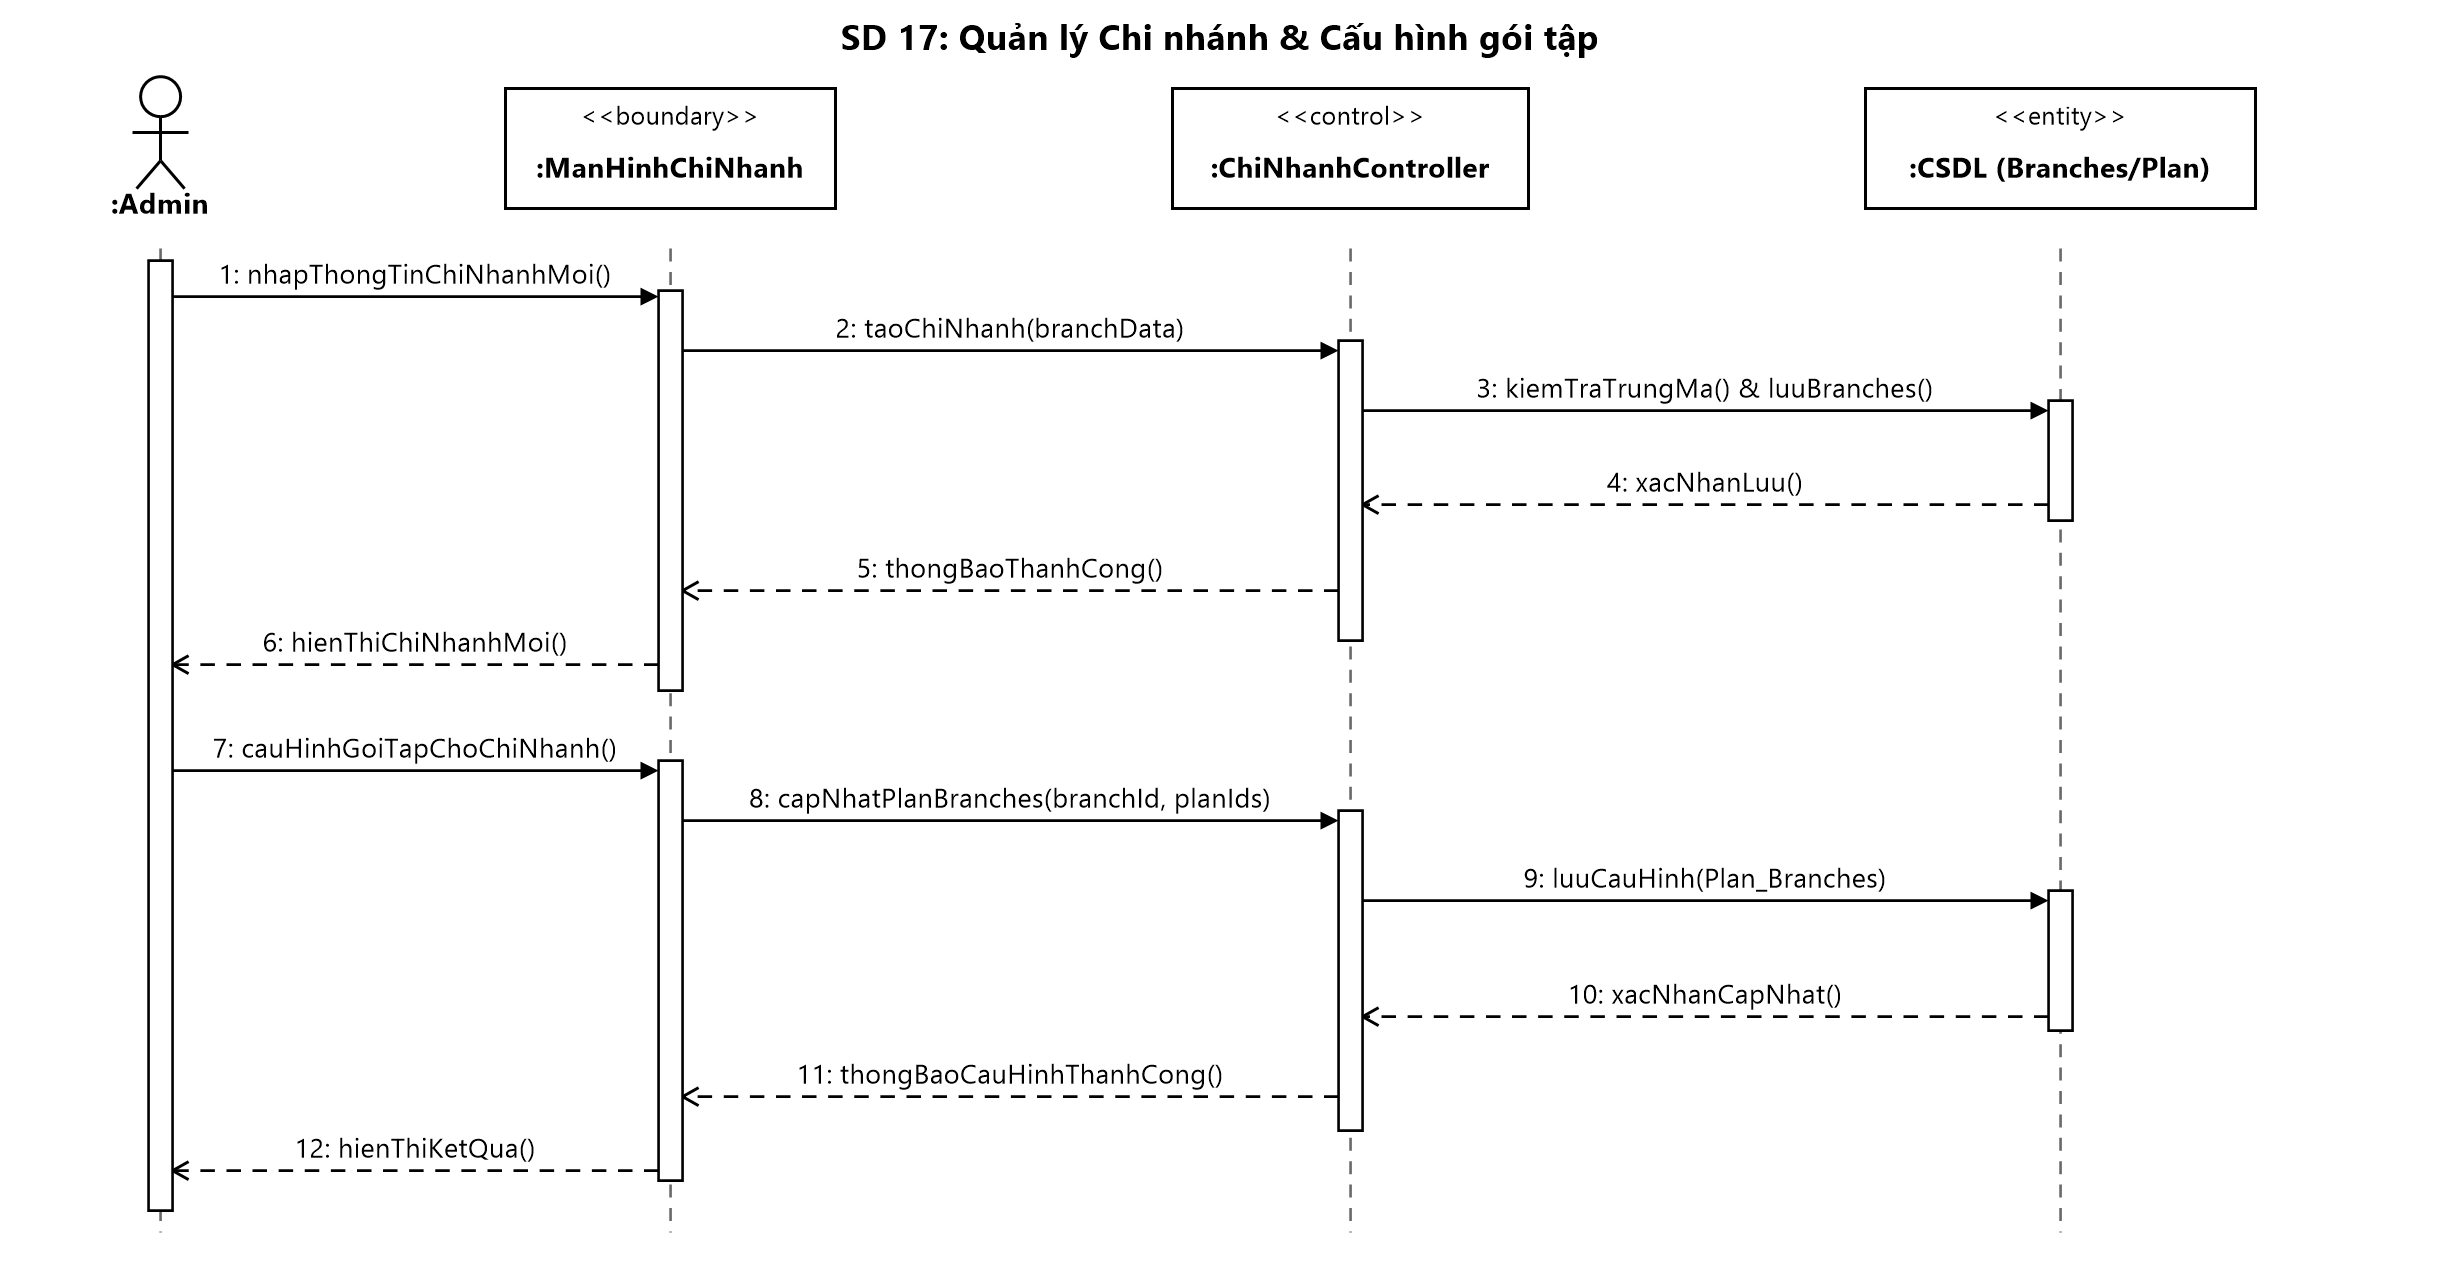
\includegraphics[width=0.95\textwidth, height=0.78\textheight, keepaspectratio]{images/sd_p61_1.png}
\caption{Sequence Diagram 17: Quản lý chi nhánh \& Cấu hình gói tập}
\end{figure}

\begin{figure}[H]
\centering
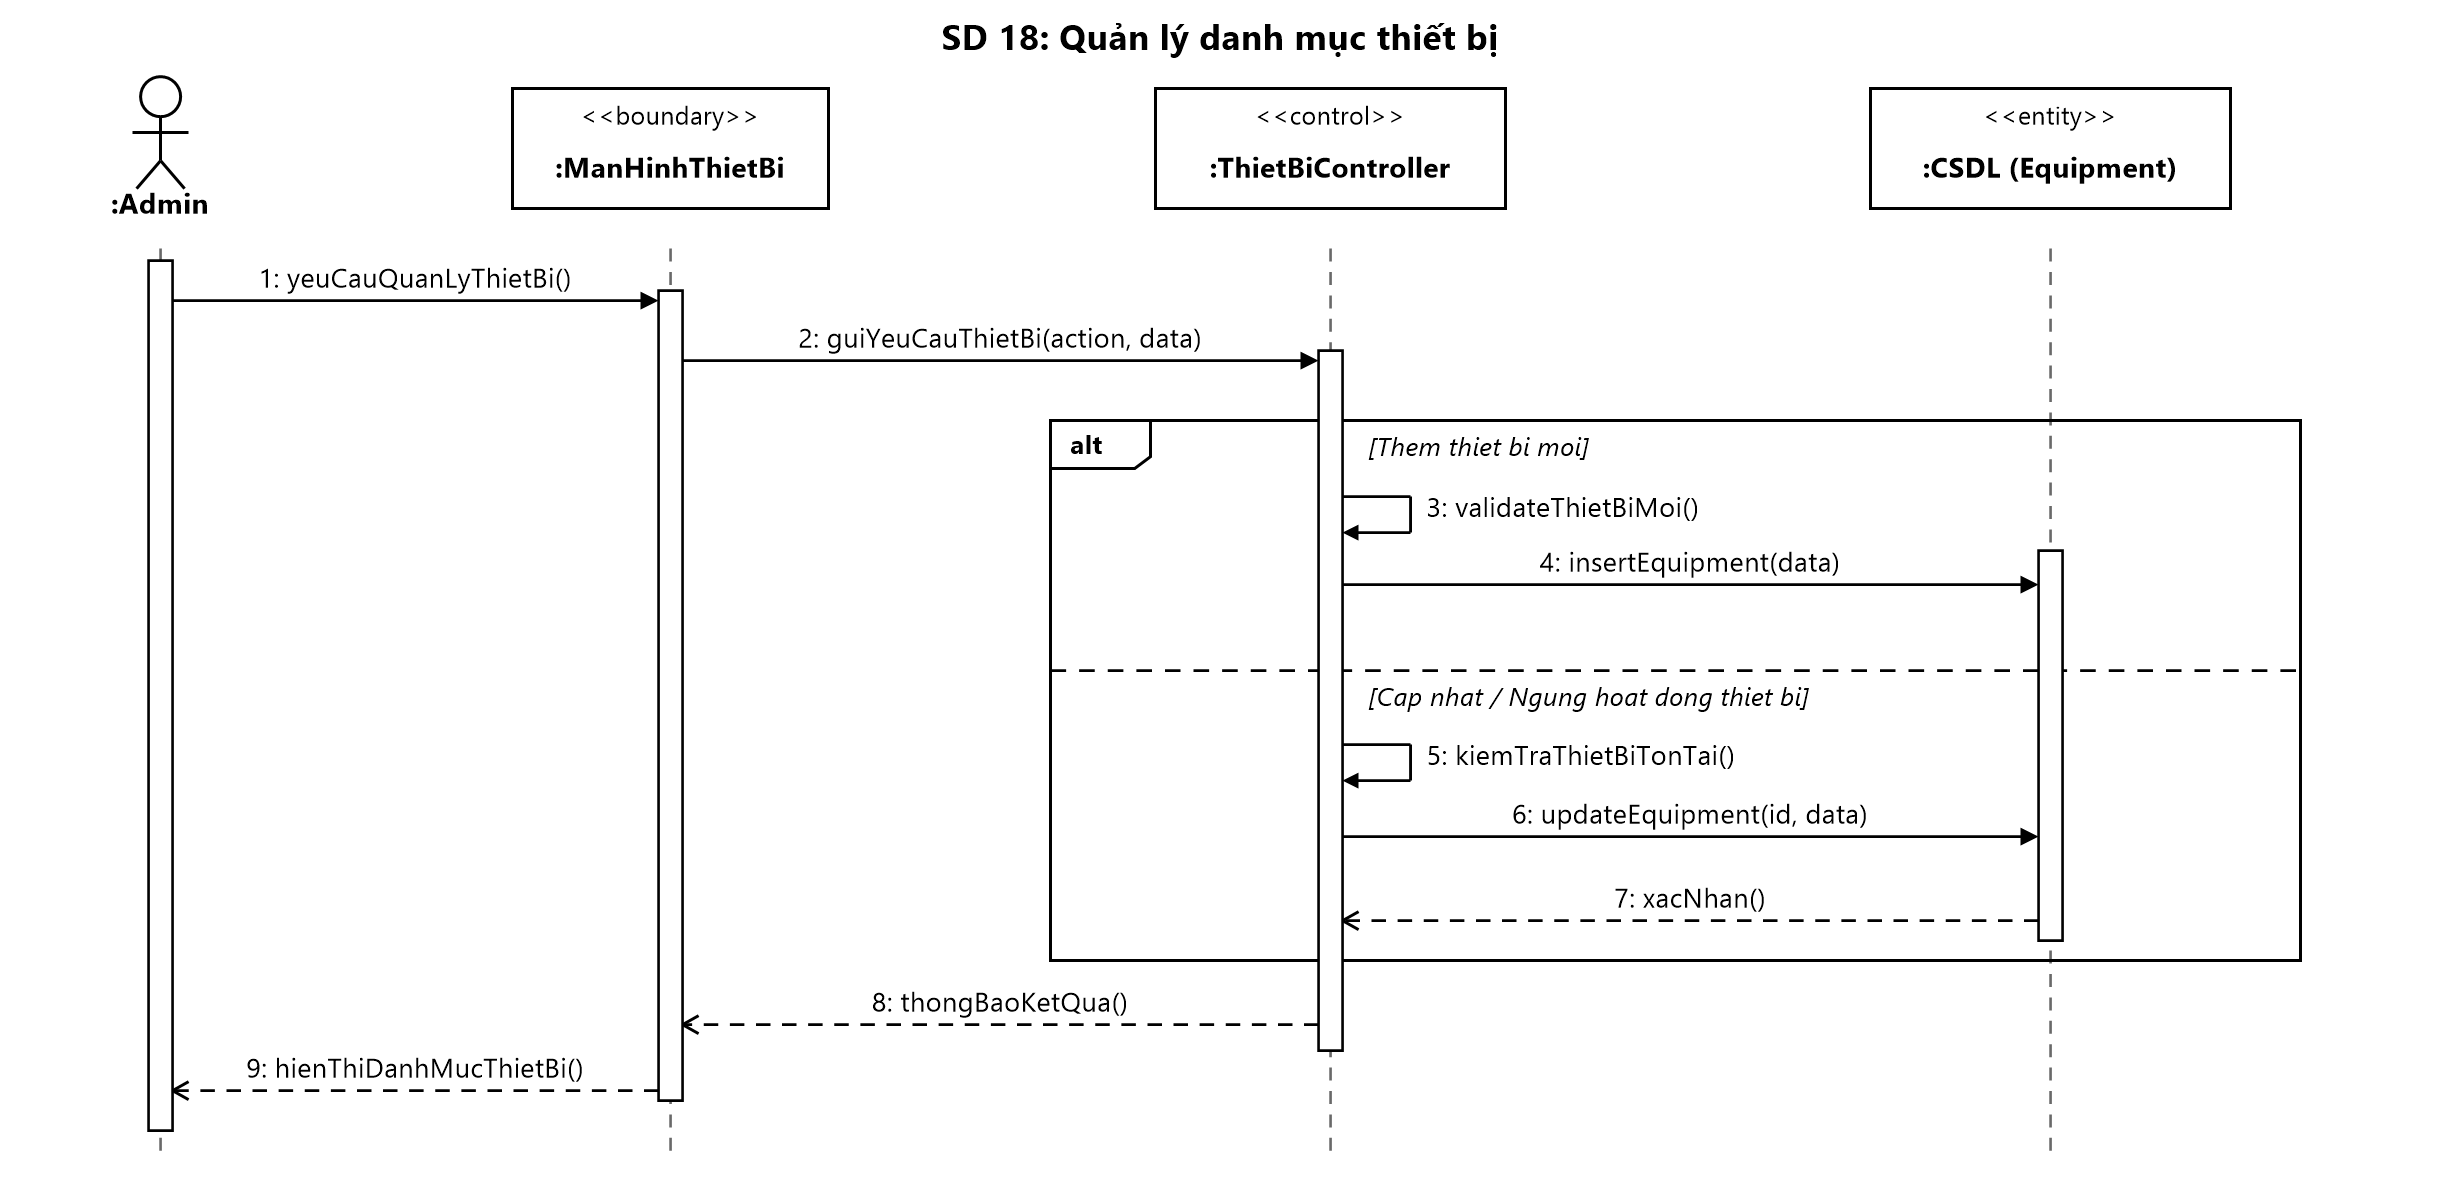
\includegraphics[width=0.95\textwidth, height=0.78\textheight, keepaspectratio]{images/sd_p62_1.png}
\caption{Sequence Diagram 18: Quản lý danh mục thiết bị}
\end{figure}

\begin{figure}[H]
\centering
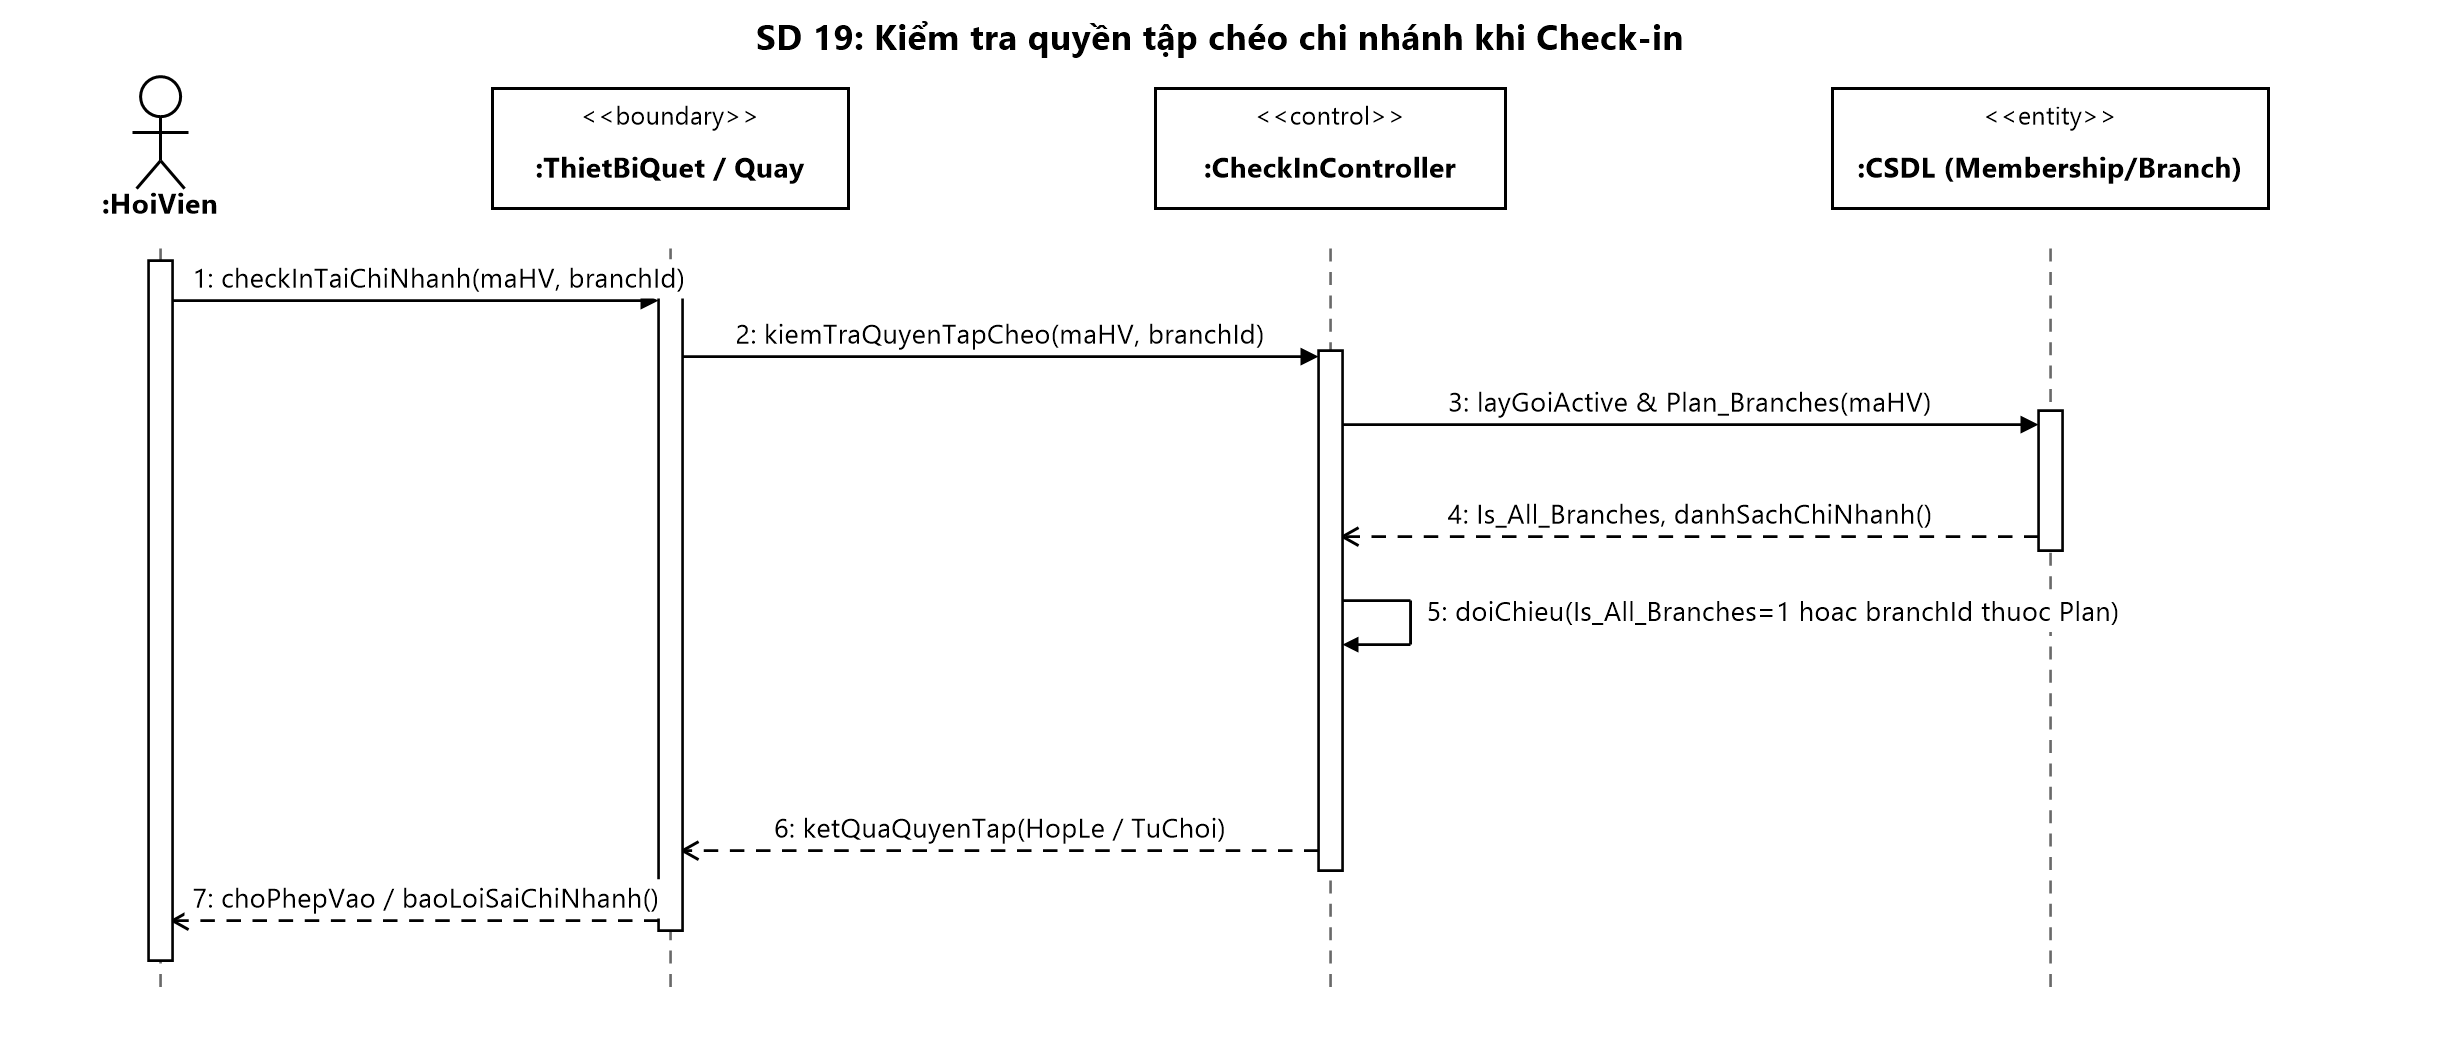
\includegraphics[width=0.95\textwidth, height=0.78\textheight, keepaspectratio]{images/sd_p62_2.png}
\caption{Sequence Diagram 19: Kiểm tra quyền tập chéo chi nhánh}
\end{figure}

\begin{figure}[H]
\centering
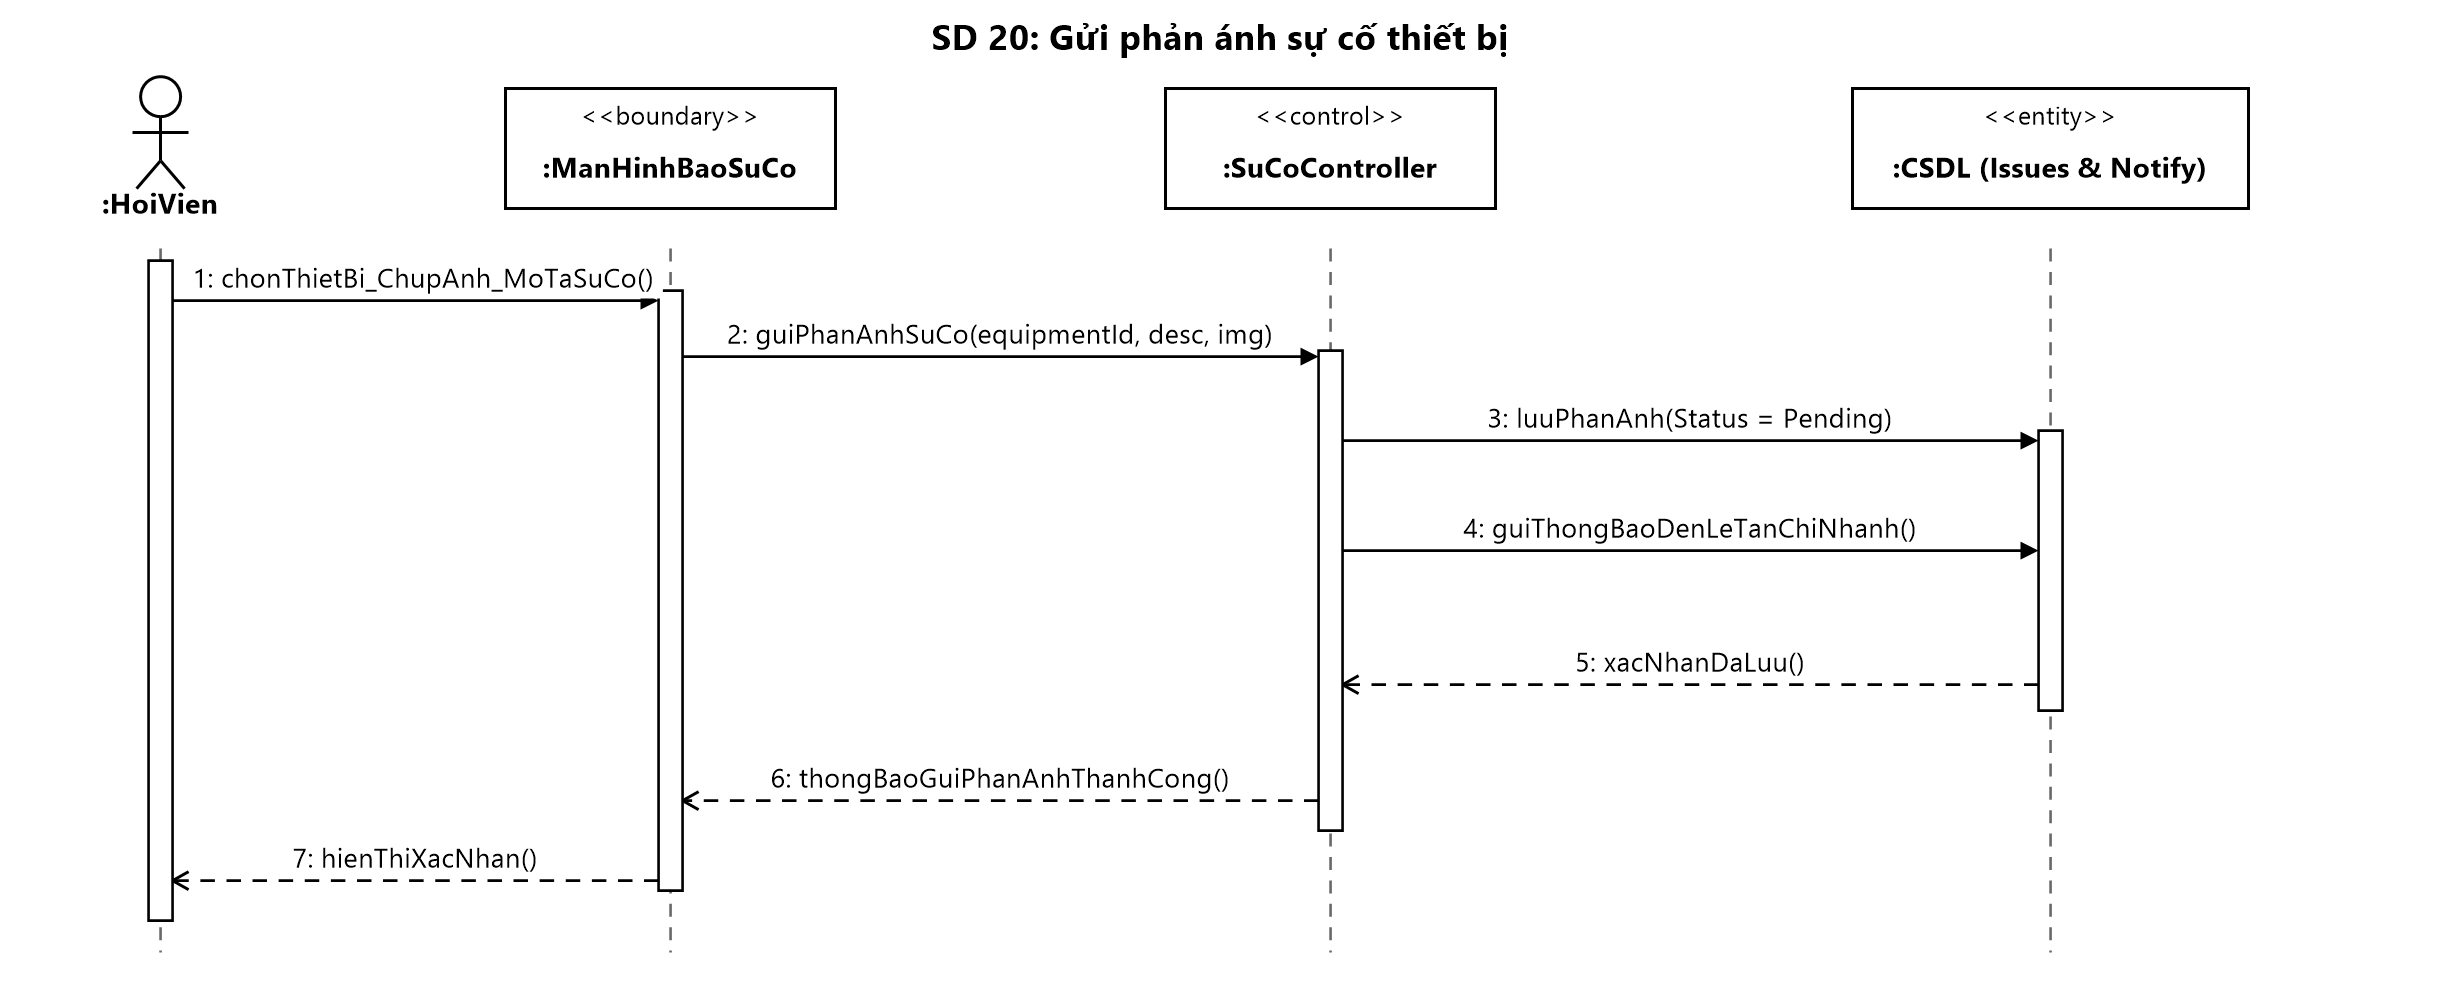
\includegraphics[width=0.95\textwidth, height=0.78\textheight, keepaspectratio]{images/sd_p63_1.png}
\caption{Sequence Diagram 20: Gửi phản ánh sự cố thiết bị}
\end{figure}

\begin{figure}[H]
\centering
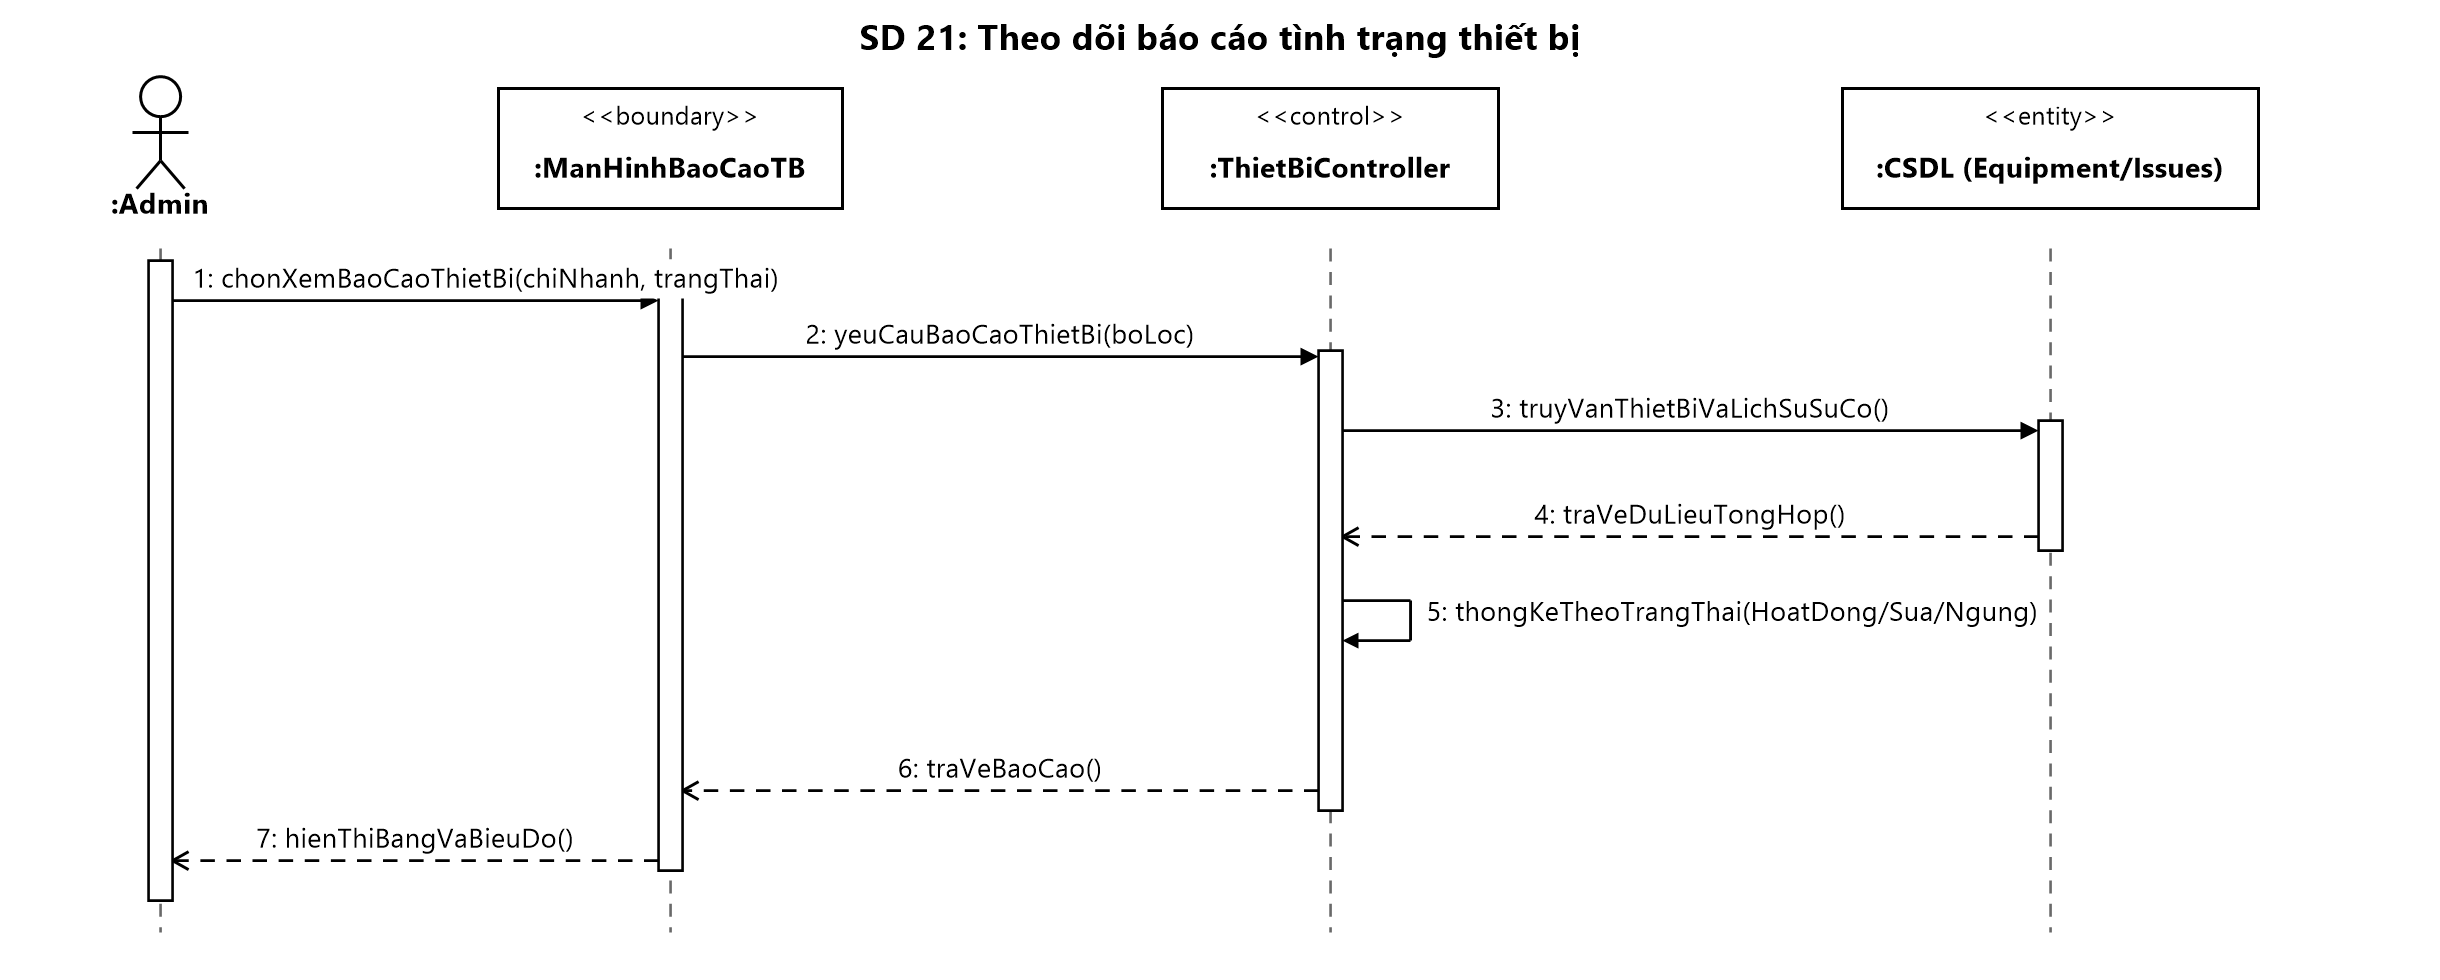
\includegraphics[width=0.95\textwidth, height=0.78\textheight, keepaspectratio]{images/sd_p63_2.png}
\caption{Sequence Diagram 21: Báo cáo tình trạng thiết bị}
\end{figure}

\begin{figure}[H]
\centering
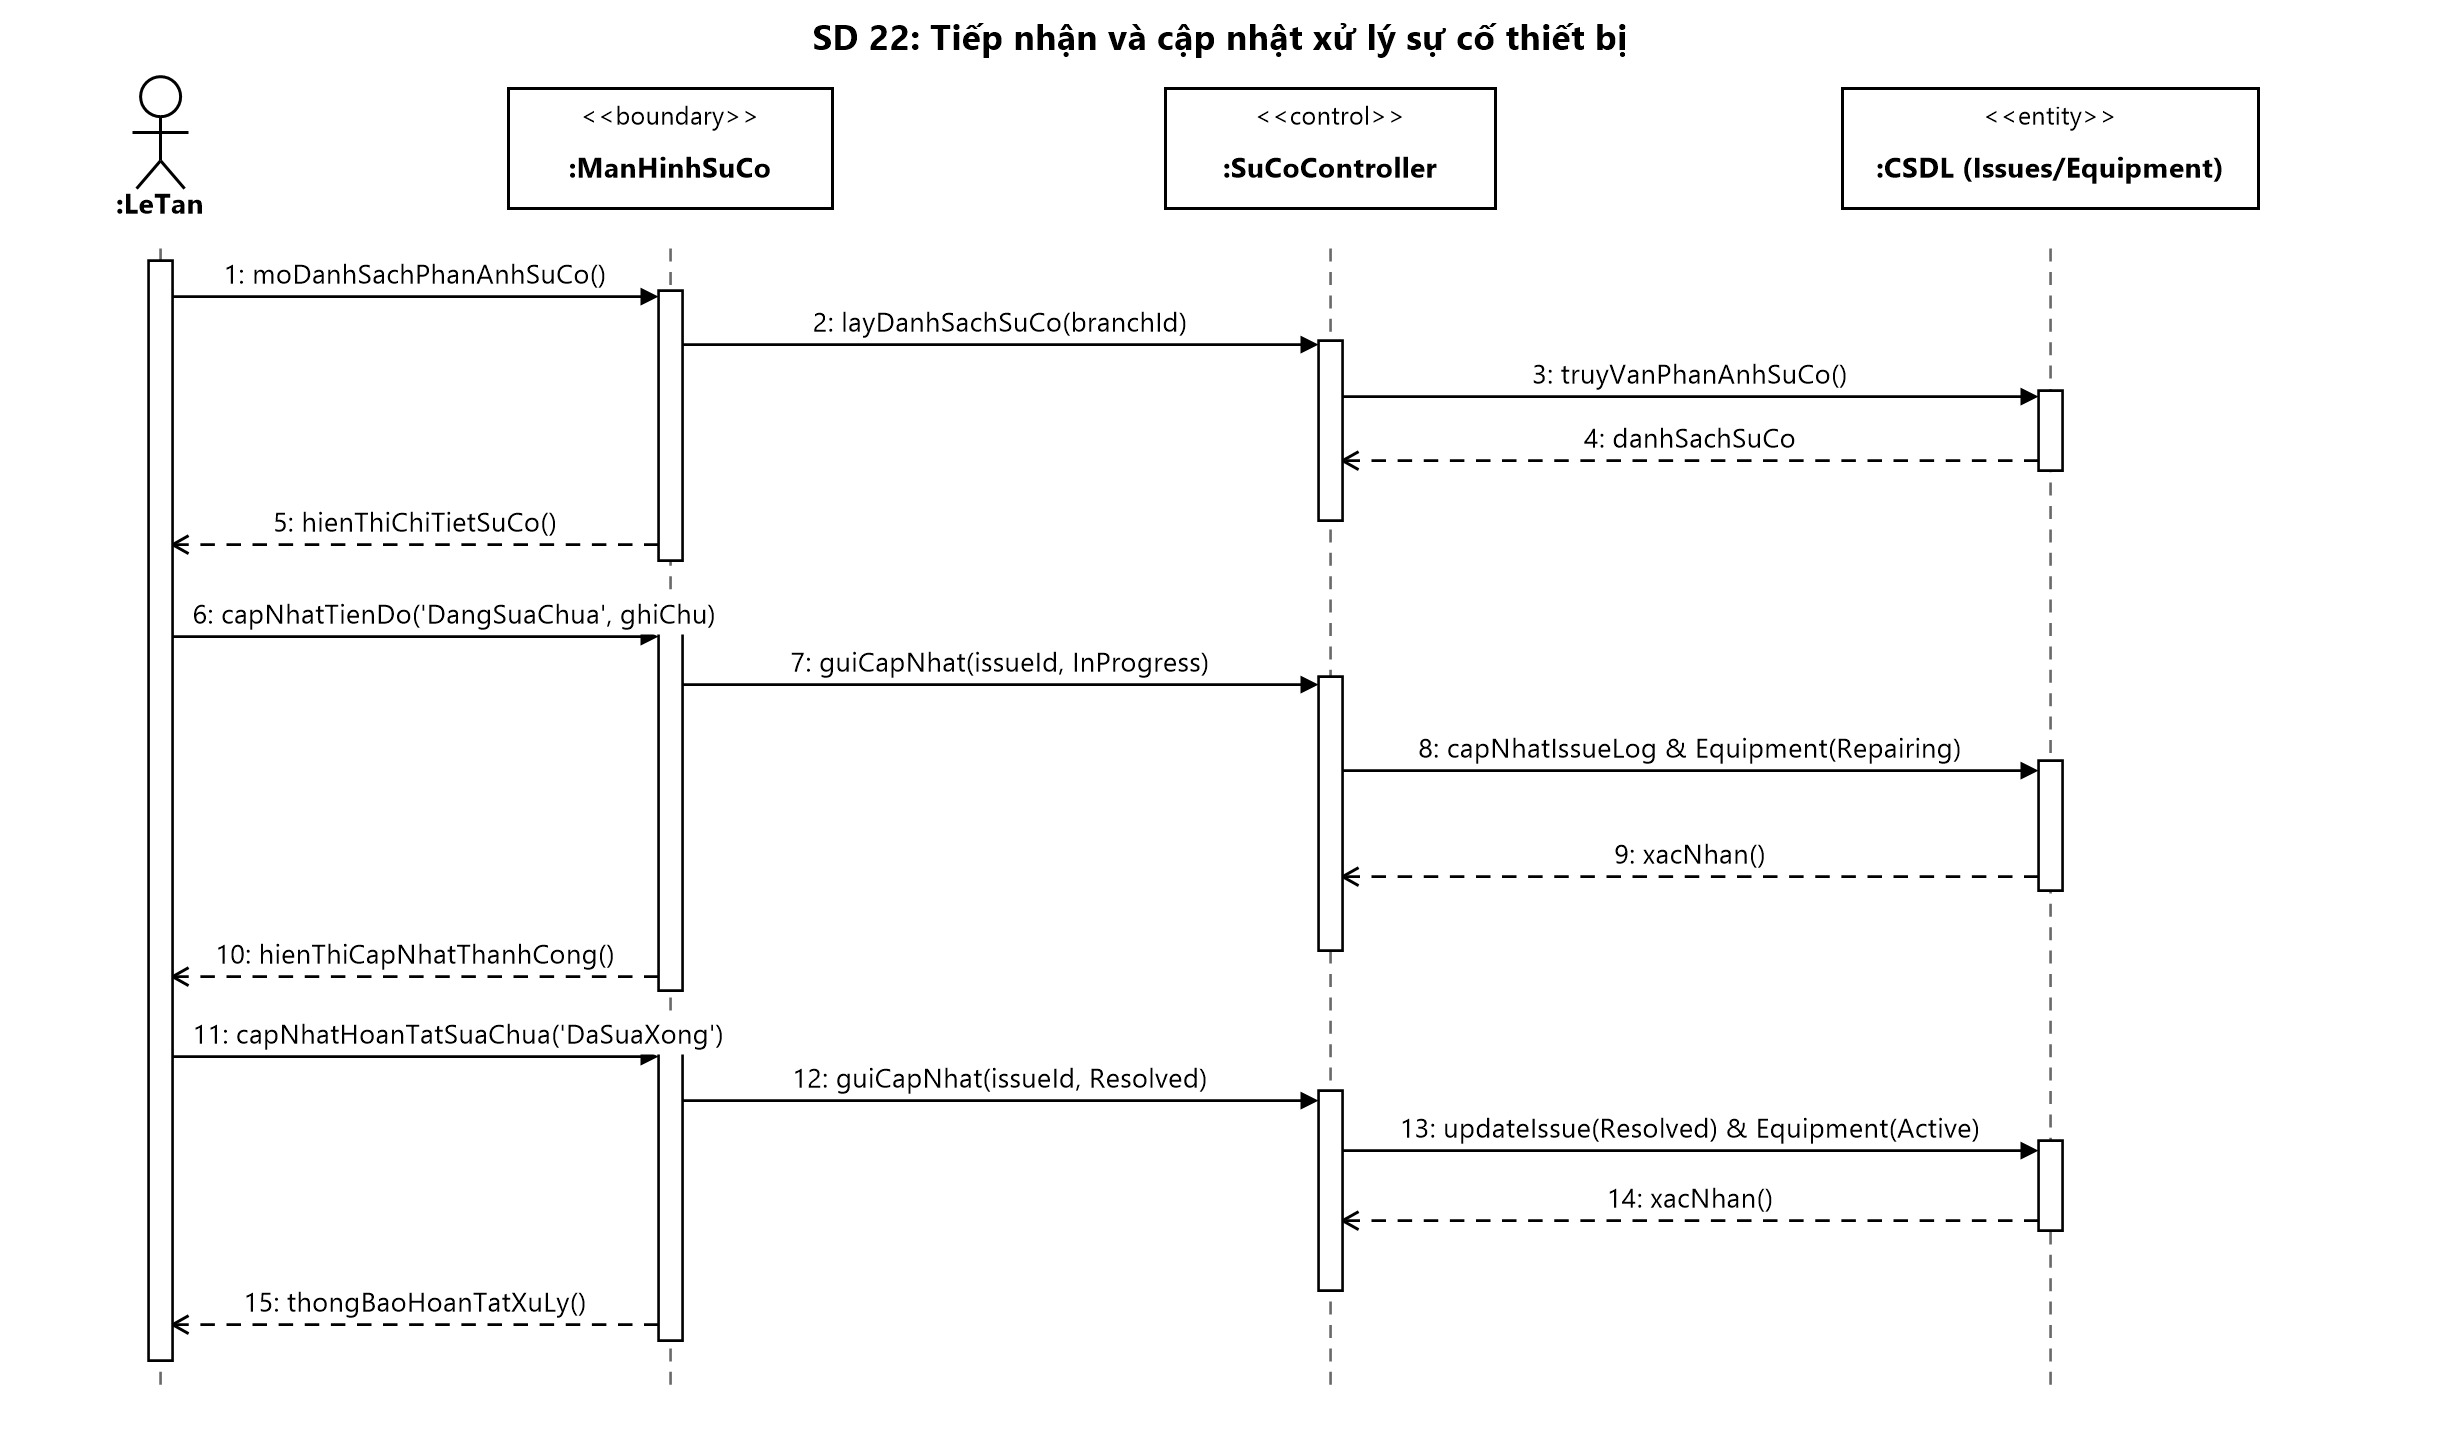
\includegraphics[width=0.95\textwidth, height=0.78\textheight, keepaspectratio]{images/sd_p64_1.png}
\caption{Sequence Diagram 22: Tiếp nhận và cập nhật xử lý sự cố}
\end{figure}

\subsubsection{Nhóm luồng Tài khoản, Bảo lưu (Freeze), Thẻ hội viên \& Đánh giá}

\begin{figure}[H]
\centering
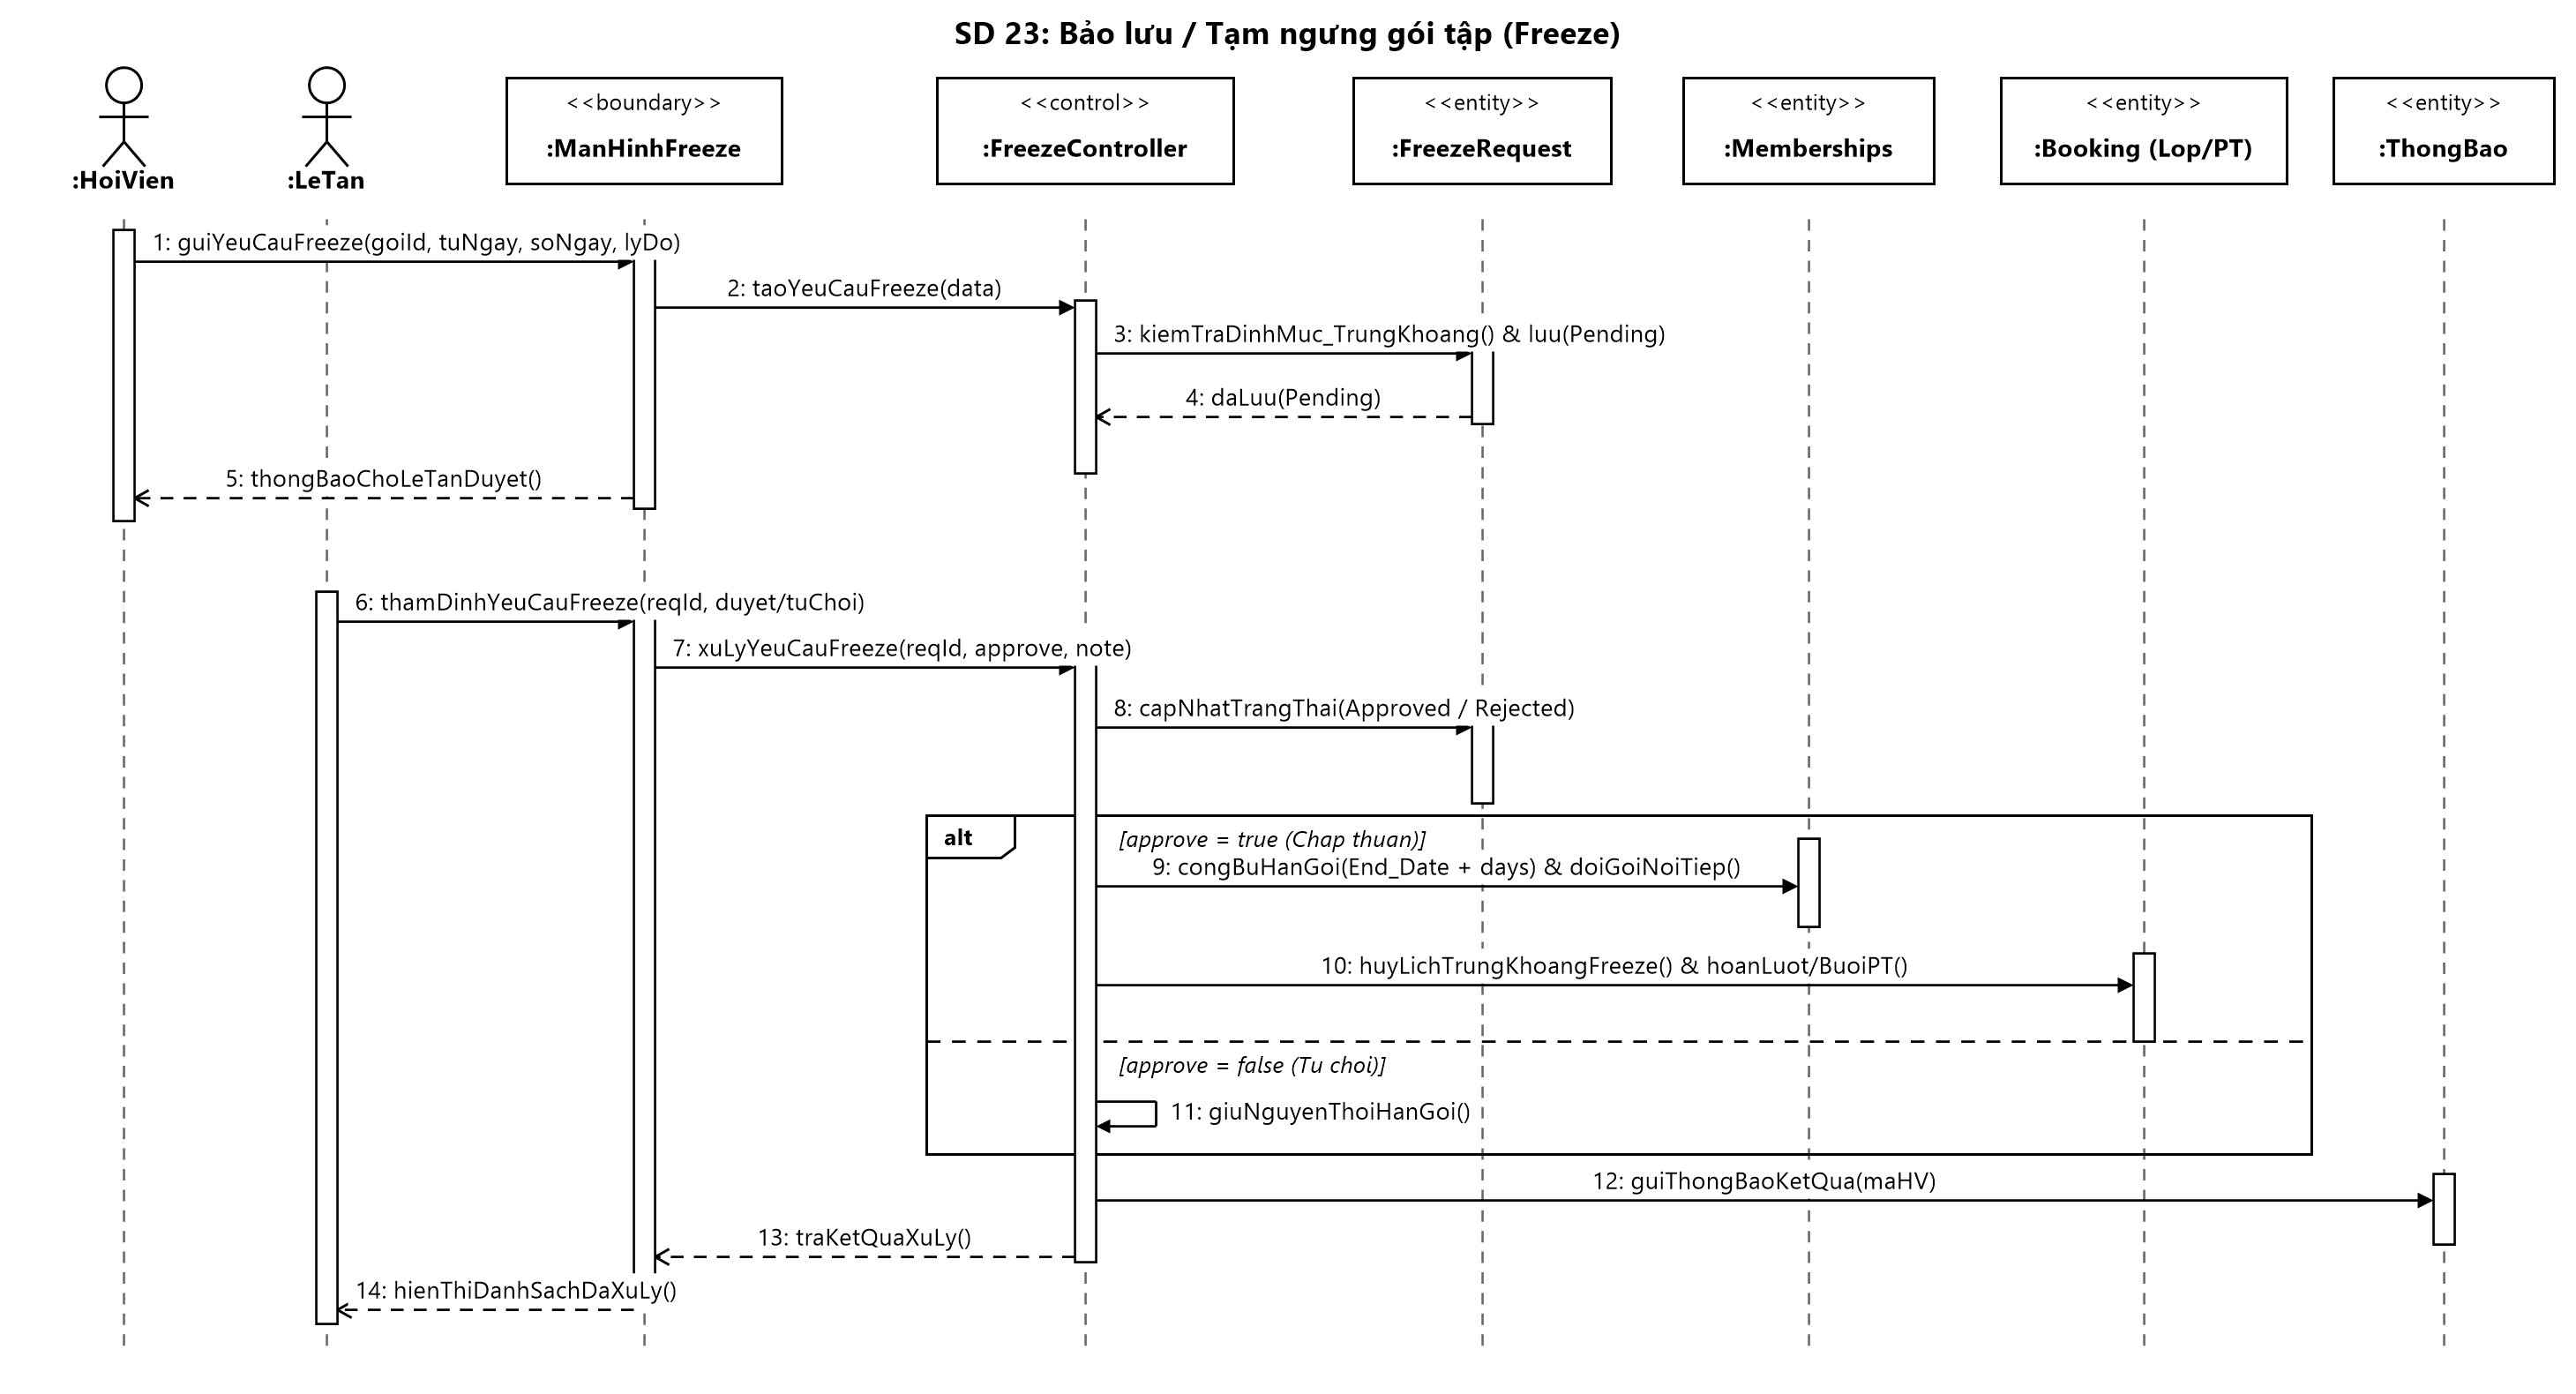
\includegraphics[width=0.95\textwidth, height=0.78\textheight, keepaspectratio]{images/sd_freeze.png}
\caption{Sequence Diagram 23: Bảo lưu / Tạm ngưng gói tập (Freeze)}
\end{figure}

\begin{figure}[H]
\centering
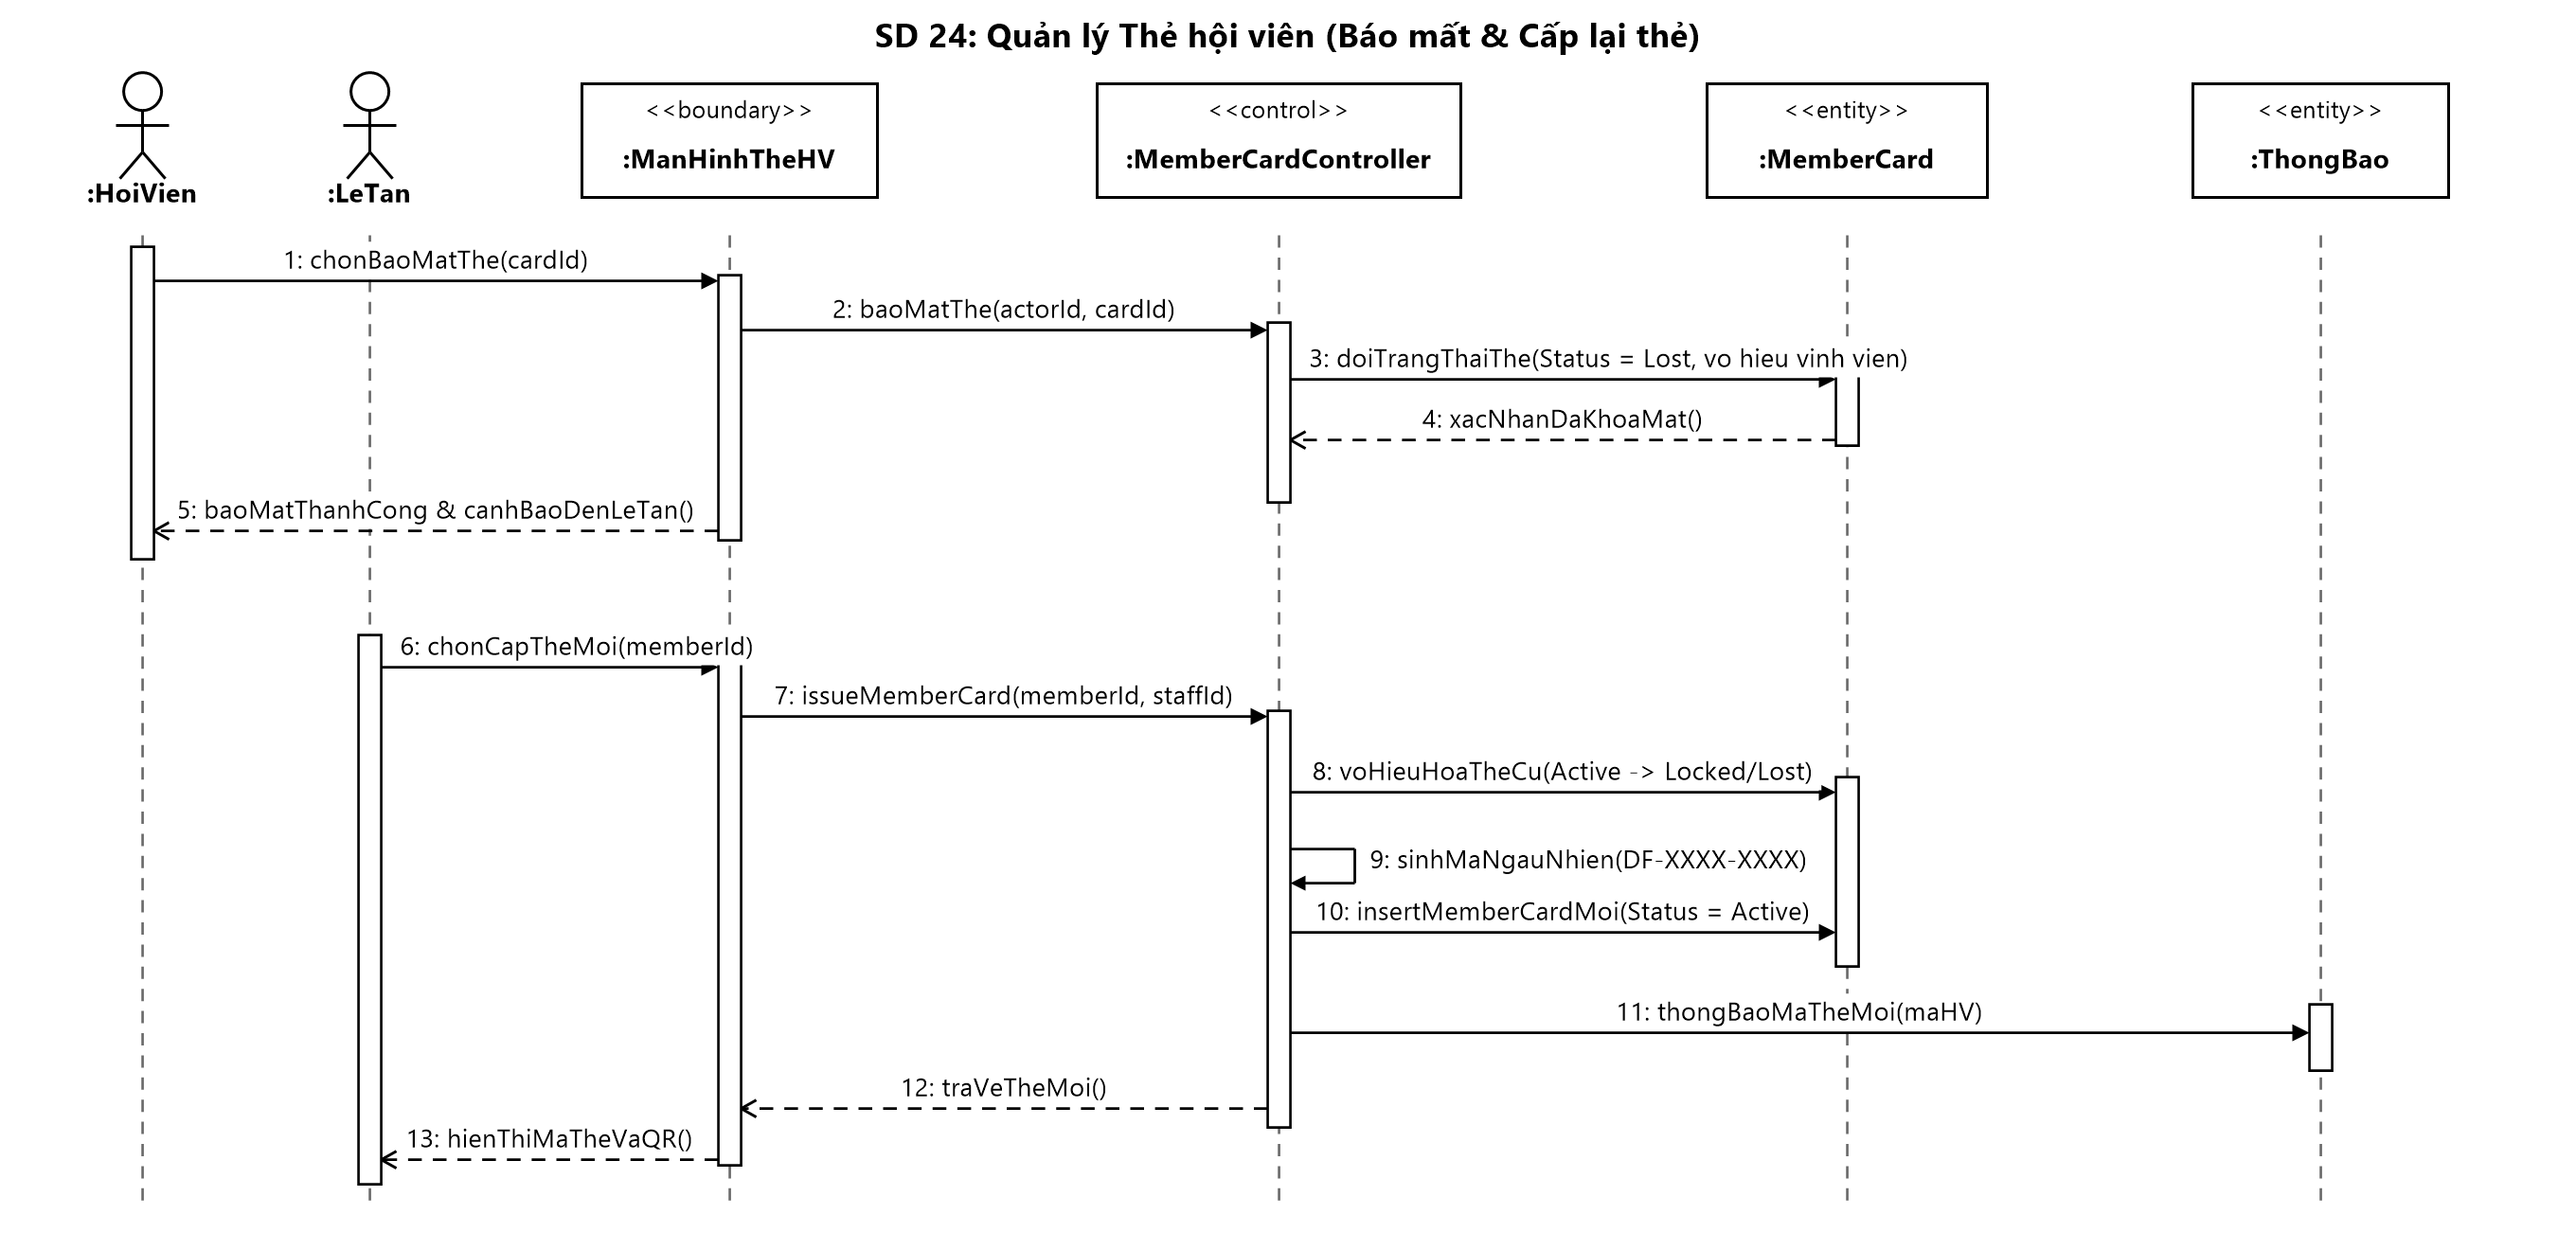
\includegraphics[width=0.95\textwidth, height=0.78\textheight, keepaspectratio]{images/sd_member_card.png}
\caption{Sequence Diagram 24: Quản lý Thẻ hội viên (Báo mất \& Cấp lại thẻ)}
\end{figure}

\begin{figure}[H]
\centering
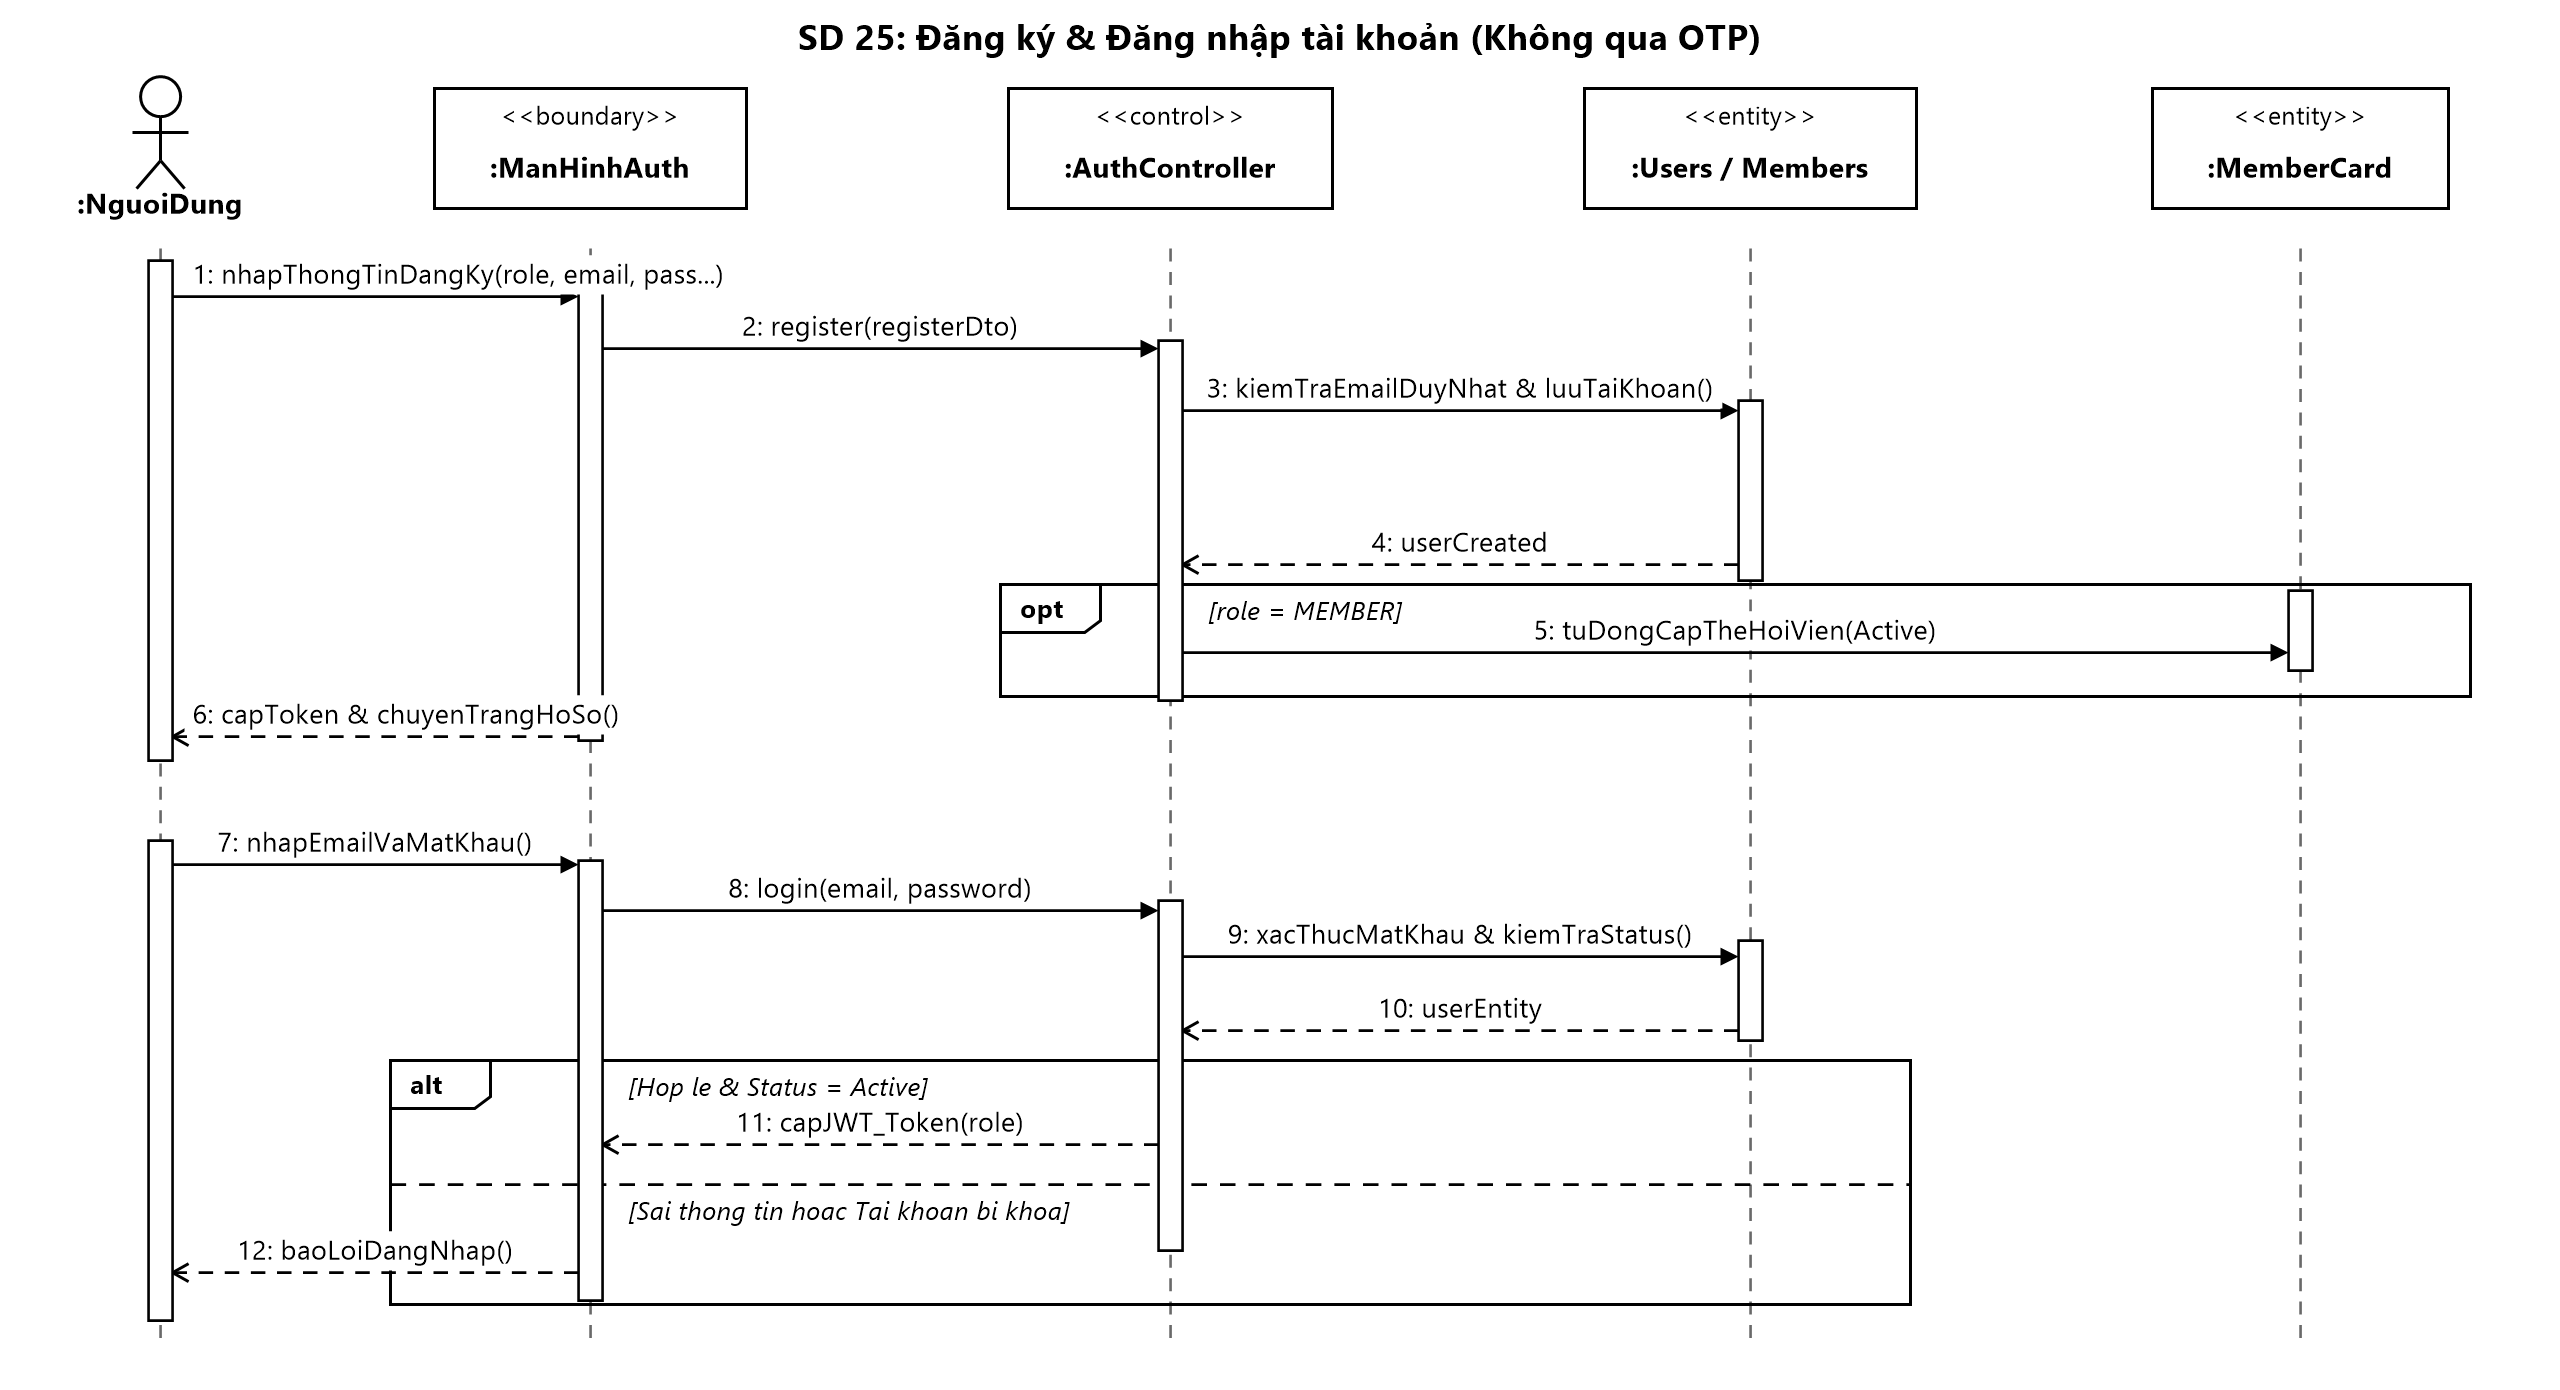
\includegraphics[width=0.95\textwidth, height=0.78\textheight, keepaspectratio]{images/sd_auth.png}
\caption{Sequence Diagram 25: Đăng ký \& Đăng nhập tài khoản}
\end{figure}

\begin{figure}[H]
\centering
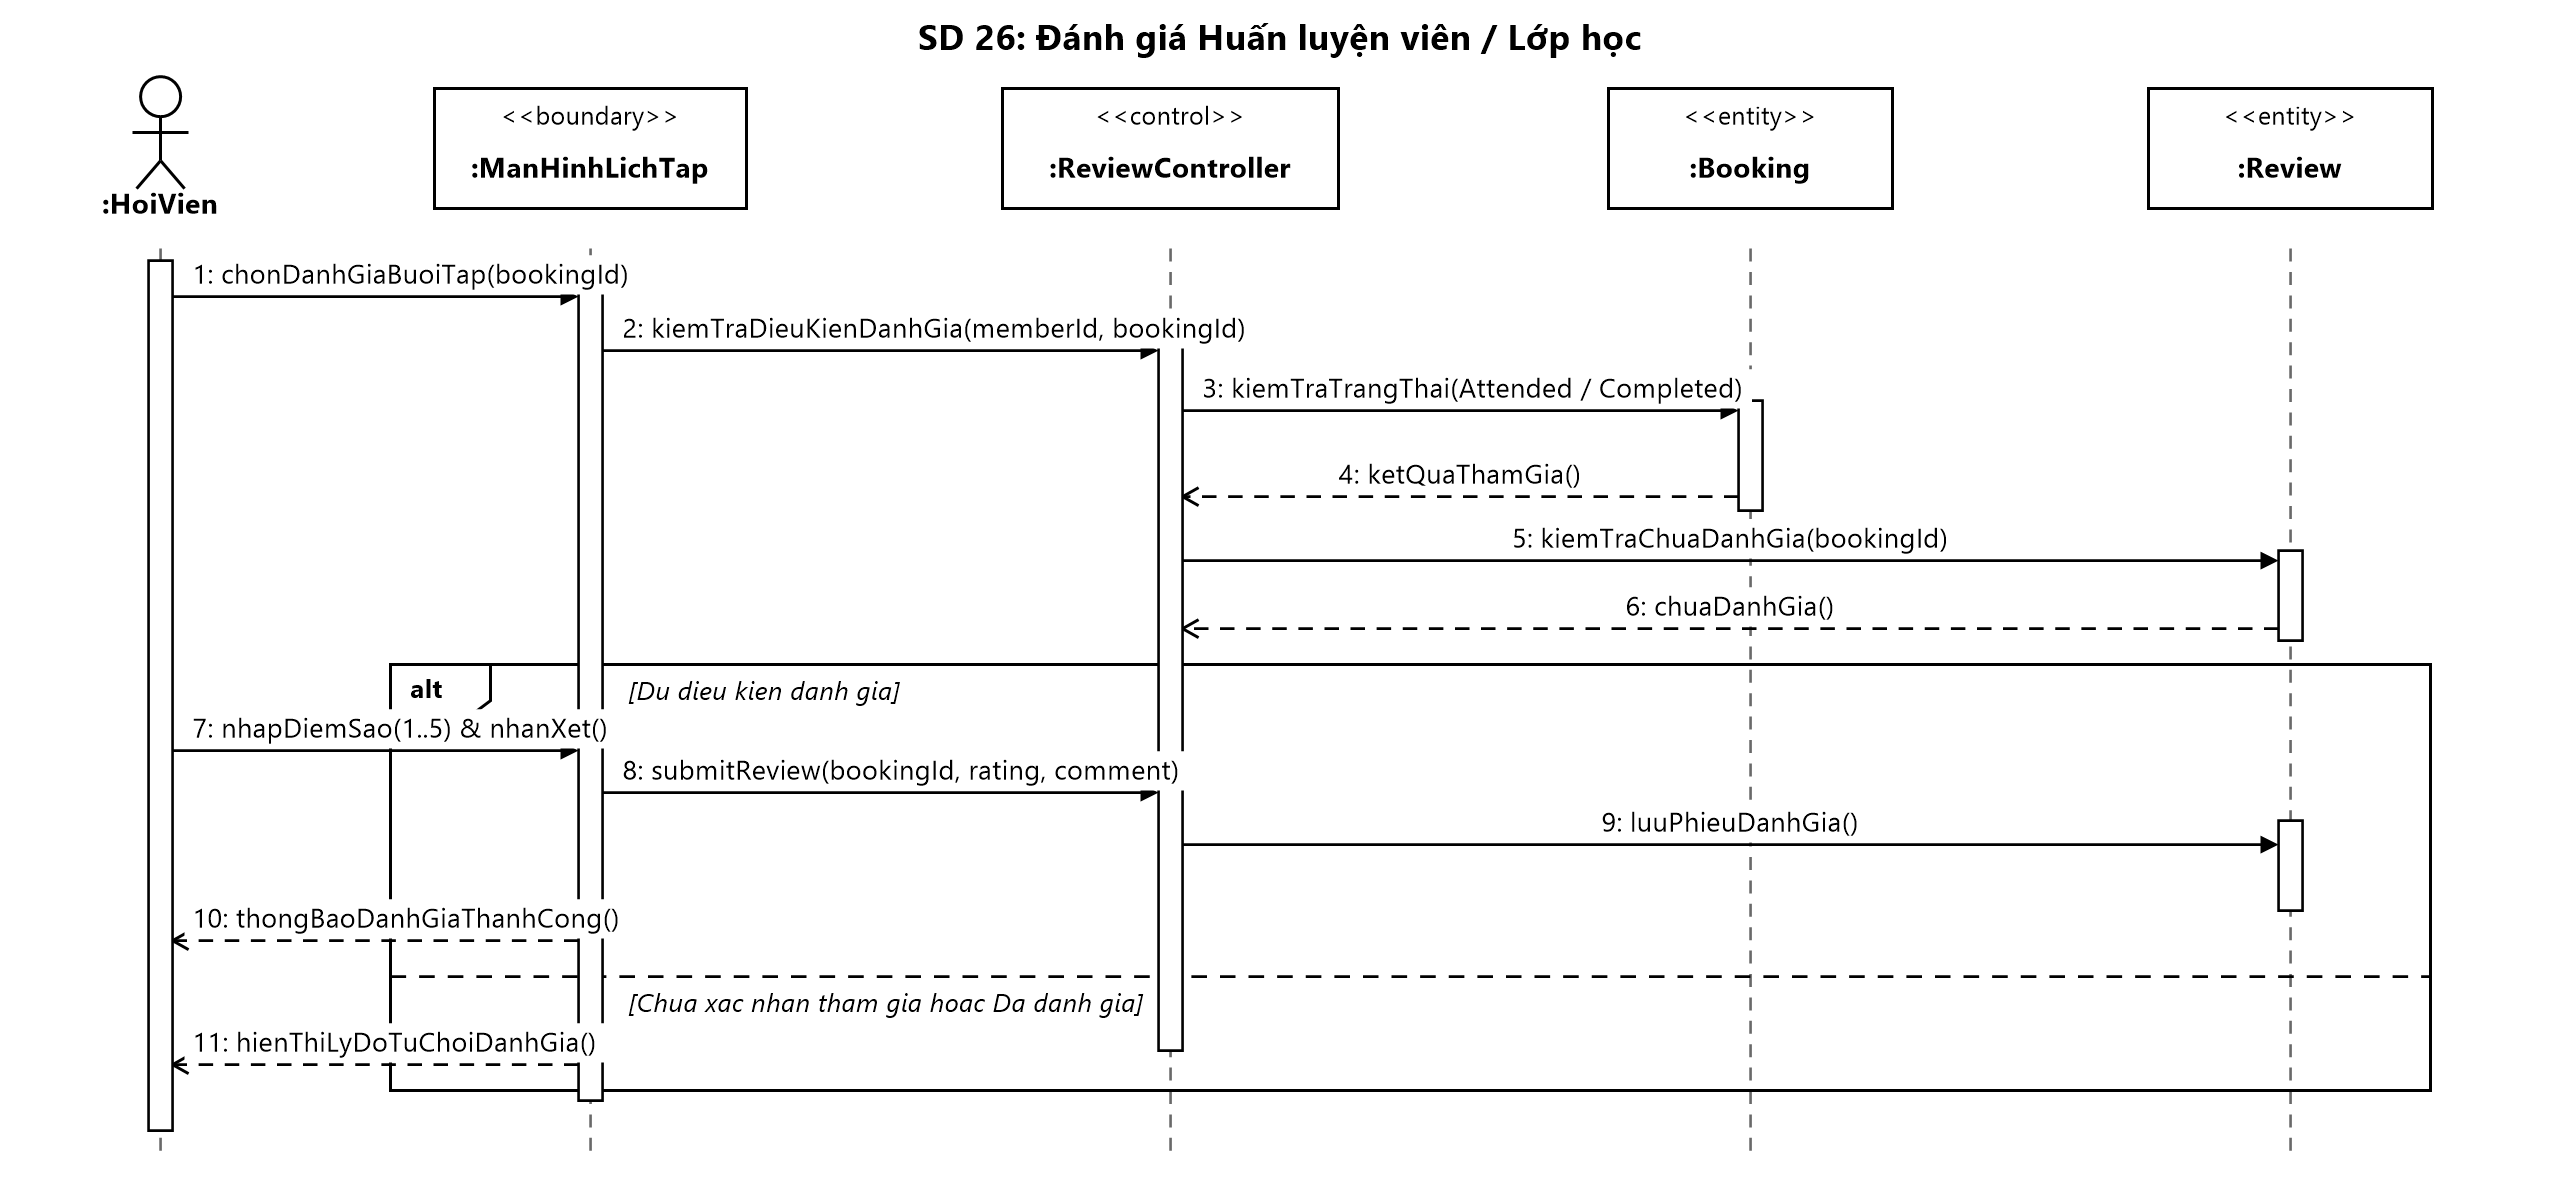
\includegraphics[width=0.95\textwidth, height=0.78\textheight, keepaspectratio]{images/sd_review.png}
\caption{Sequence Diagram 26: Đánh giá Huấn luyện viên / Lớp học}
\end{figure}

% ==============================================================================
% 3. PHÂN TÍCH
% ==============================================================================
\newpage
\section{Phân tích}

\subsection{Sơ đồ lớp (Class Diagram)}

\subsubsection{Sơ đồ lớp mức phân tích}
Sơ đồ lớp mức phân tích của hệ thống \textbf{DFGymCenter} mô tả cấu trúc tĩnh gồm \textbf{24 lớp đối tượng} (bao gồm lớp \texttt{MemberCard} quản lý thẻ hội viên) và \textbf{35 mối quan hệ} giữa các lớp.

\begin{figure}[H]
\centering
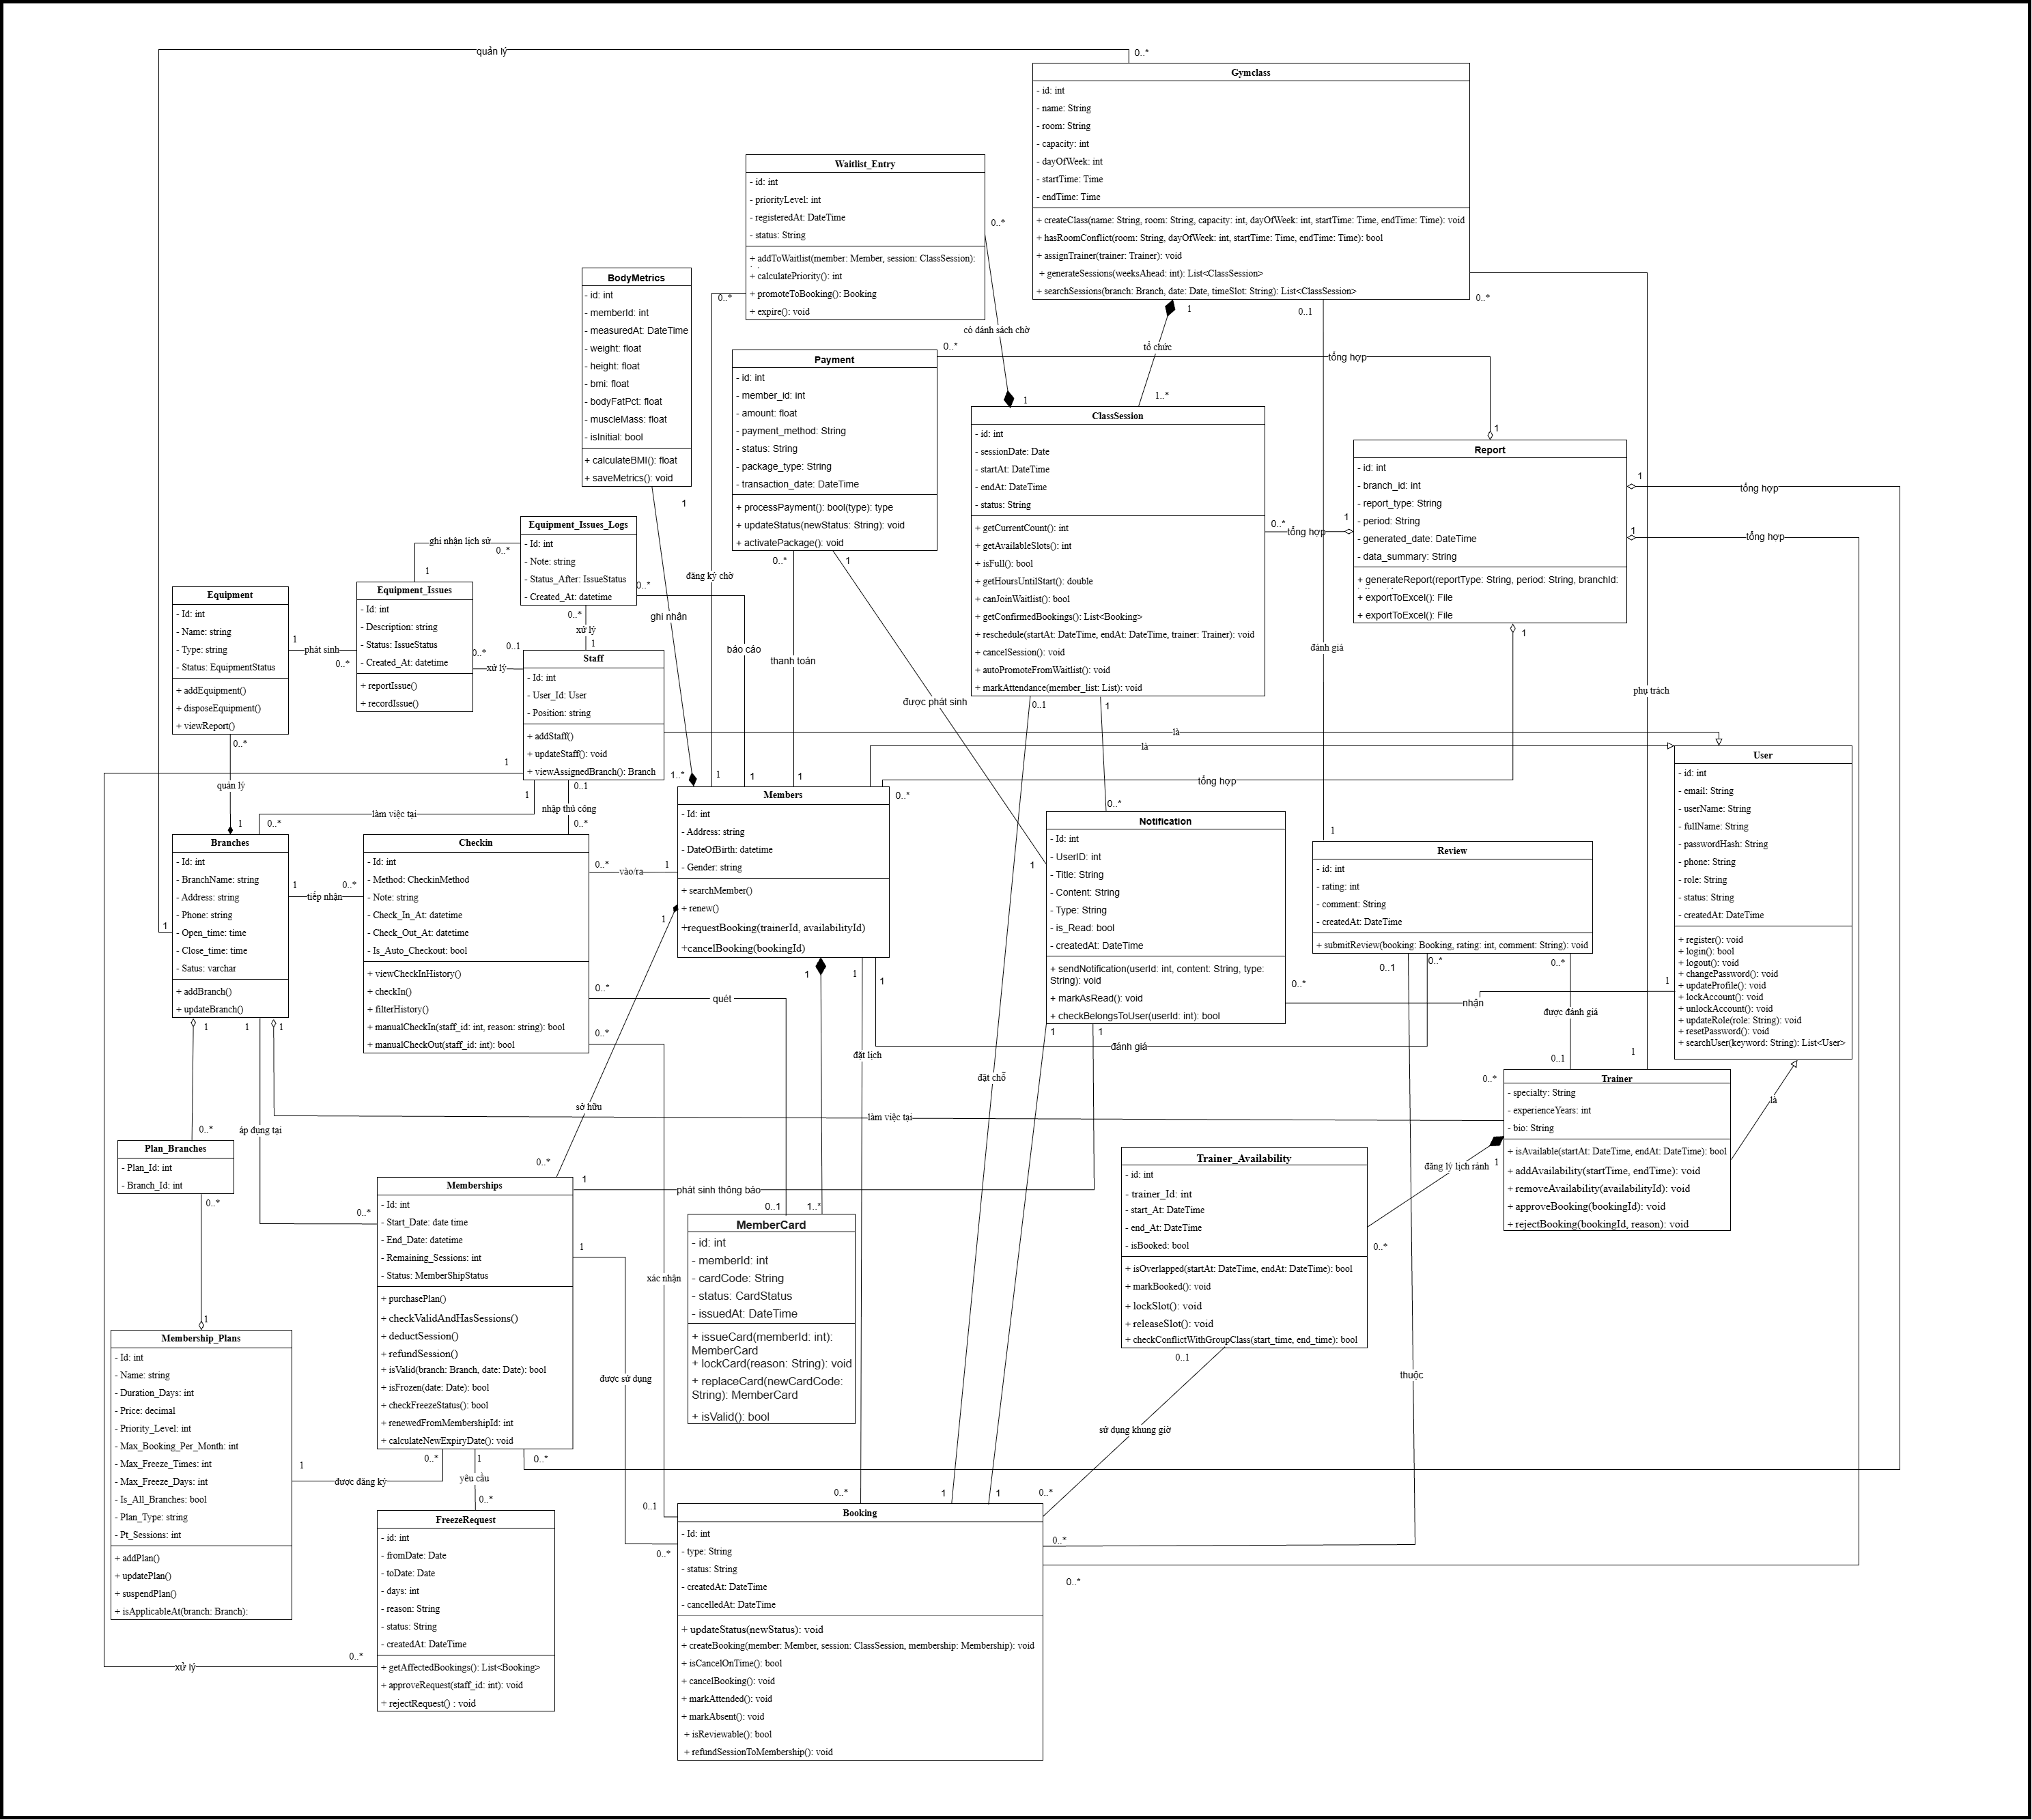
\includegraphics[width=\textwidth, height=0.80\textheight, keepaspectratio]{images/class_p03_1.png}
\caption{Sơ đồ lớp mức phân tích hệ thống DFGymCenter}
\end{figure}

\subsubsection{Danh sách các lớp đối tượng và quan hệ}

{\small
\setlength{\tabcolsep}{4pt}
\begin{longtable}{|c|L{3.7cm}|L{2.7cm}|L{8.2cm}|}
\hline
\textbf{STT} & \textbf{Tên lớp} & \textbf{Loại} & \textbf{Ý nghĩa / Ghi chú} \\ \hline
\endfirsthead
\hline
\textbf{STT} & \textbf{Tên lớp} & \textbf{Loại} & \textbf{Ý nghĩa / Ghi chú} \\ \hline
\endhead
\hline
\endfoot
\hline
\caption{Danh sách các lớp đối tượng trong hệ thống DFGymCenter} \\
\endlastfoot
1 & \texttt{User} & Lớp đối tượng & Đại diện tài khoản/người dùng chung của hệ thống. \\ \hline
2 & \texttt{Members} & Lớp đối tượng & Đại diện hội viên sử dụng dịch vụ phòng Gym; kế thừa \texttt{User}. \\ \hline
3 & \texttt{Trainer} & Lớp đối tượng & Đại diện huấn luyện viên; kế thừa \texttt{User}. \\ \hline
4 & \texttt{Staff} & Lớp đối tượng & Đại diện nhân viên phòng Gym; kế thừa \texttt{User}. \\ \hline
5 & \texttt{Branches} & Lớp đối tượng & Thông tin chi nhánh phòng Gym. \\ \hline
6 & \texttt{Equipment} & Lớp đối tượng & Thông tin thiết bị tại chi nhánh. \\ \hline
7 & \texttt{Equipment\_Issues} & Lớp đối tượng & Thông tin sự cố/báo hỏng thiết bị. \\ \hline
8 & \texttt{Equipment\_Issues\_Logs} & Lớp đối tượng & Lịch sử cập nhật trạng thái xử lý sự cố thiết bị. \\ \hline
9 & \texttt{BodyMetrics} & Lớp đối tượng & Các chỉ số cơ thể được ghi nhận của hội viên. \\ \hline
10 & \texttt{Payment} & Lớp đối tượng & Giao dịch thanh toán liên quan đến gói tập. \\ \hline
11 & \texttt{Notification} & Lớp đối tượng & Thông báo gửi đến người dùng. \\ \hline
12 & \texttt{Report} & Lớp đối tượng & Báo cáo tổng hợp động theo chi nhánh và kỳ báo cáo (Read Model kết xuất Excel/PDF tức thời, không lưu thành bảng hay lưu file vào CSDL để tránh nặng hệ thống). \\ \hline
13 & \texttt{GymClass} & Lớp đối tượng & Thông tin lớp tập nhóm được tổ chức tại chi nhánh. \\ \hline
14 & \texttt{ClassSession} & Lớp đối tượng & Một buổi học cụ thể thuộc lớp \texttt{GymClass}. \\ \hline
15 & \texttt{Waitlist\_Entry} & Lớp đối tượng & Thông tin hội viên đăng ký danh sách chờ buổi tập. \\ \hline
16 & \texttt{Trainer\_Availability} & Lớp đối tượng & Khung thời gian rảnh của huấn luyện viên. \\ \hline
17 & \texttt{Booking} & Lớp đối tượng & Thông tin đặt lịch tập của hội viên (lớp nhóm hoặc PT). \\ \hline
18 & \texttt{Checkin} & Lớp đối tượng & Ghi nhận lượt check-in/check-out của hội viên. \\ \hline
19 & \texttt{Memberships} & Lớp đối tượng & Gói tập mà hội viên đã đăng ký và đang sử dụng. \\ \hline
20 & \texttt{Membership\_Plans} & Lớp đối tượng & Danh mục các loại gói tập do phòng Gym cung cấp. \\ \hline
21 & \texttt{Plan\_Branches} & Lớp liên kết & Liên kết gói tập với các chi nhánh được áp dụng. \\ \hline
22 & \texttt{FreezeRequest} & Lớp đối tượng & Yêu cầu đóng băng/tạm dừng thời hạn gói tập. \\ \hline
23 & \texttt{Review} & Lớp đối tượng & Đánh giá của hội viên về buổi đặt lịch, HLV hoặc lớp tập. \\* \hline
24 & \texttt{MemberCard} & Lớp đối tượng & Đại diện thẻ thành viên (RFID hoặc mã QR) cấp cho hội viên để kiểm soát ra/vào và điểm danh tại các chi nhánh. \\ \hline
\end{longtable}
}

\begin{longtable}{|c|L{4.8cm}|L{2.6cm}|p{7.6cm}|}
\hline
\textbf{STT} & \textbf{Quan hệ} & \textbf{Loại} & \textbf{Ý nghĩa / Ghi chú} \\ \hline
\endfirsthead
\hline
\textbf{STT} & \textbf{Quan hệ} & \textbf{Loại} & \textbf{Ý nghĩa / Ghi chú} \\ \hline
\endhead
\hline
\endfoot
\hline
\caption{Danh sách các mối quan hệ giữa các lớp đối tượng} \\
\endlastfoot
1 & \texttt{User -- Members} & Generalization & \texttt{Members} là một loại \texttt{User}; thừa hưởng thông tin và hành vi chung. \\ \hline
2 & \texttt{User -- Trainer} & Generalization & \texttt{Trainer} là một loại \texttt{User}; bổ sung chuyên môn và lịch rảnh. \\ \hline
3 & \texttt{User -- Staff} & Generalization & \texttt{Staff} là một loại \texttt{User}; bổ sung vị trí công việc và chi nhánh. \\ \hline
4 & \texttt{Members -- BodyMetrics} & Composition & Hội viên có nhiều bản ghi chỉ số cơ thể theo thời gian. \\ \hline
5 & \texttt{Members -- Memberships} & Composition & Hội viên đăng ký và sở hữu các gói tập. \\ \hline
6 & \texttt{Members -- Booking} & Association & Hội viên thực hiện các lượt đặt lịch. \\ \hline
7 & \texttt{Members -- Checkin} & Association & Hội viên có lịch sử check-in/check-out. \\ \hline
8 & \texttt{Members -- Waitlist\_Entry} & Association & Hội viên đăng ký vào danh sách chờ. \\ \hline
9 & \texttt{Members -- Review} & Association & Hội viên viết đánh giá. \\ \hline
10 & \texttt{Members -- Payment} & Association & Hội viên phát sinh giao dịch thanh toán. \\ \hline
11 & \texttt{User -- Notification} & Association & Người dùng nhận các thông báo hệ thống. \\ \hline
12 & \texttt{Staff -- Branches} & Association & Nhân viên làm việc tại chi nhánh được phân công. \\ \hline
13 & \texttt{Trainer -- Branches} & Aggregation & Huấn luyện viên làm việc tại chi nhánh. \\ \hline
14 & \texttt{Trainer -- Trainer\_Availability} & Composition & Huấn luyện viên đăng ký các khung giờ rảnh. \\ \hline
15 & \texttt{Trainer -- GymClass} & Association & Huấn luyện viên phụ trách lớp tập nhóm. \\ \hline
16 & \texttt{Branches -- GymClass} & Association & Chi nhánh quản lý/tổ chức các lớp tập. \\ \hline
17 & \texttt{GymClass -- ClassSession} & Composition & Một lớp tập bao gồm các buổi tập cụ thể. \\ \hline
18 & \texttt{ClassSession -- Waitlist\_Entry} & Composition & Buổi tập có danh sách hội viên chờ. \\ \hline
19 & \texttt{ClassSession -- Booking} & Association & Booking được tạo cho một buổi tập nhóm. \\ \hline
20 & \texttt{Trainer\_Availability -- Booking} & Association & Booking sử dụng một khung giờ rảnh của HLV. \\ \hline
21 & \texttt{Booking -- Checkin} & Association & Check-in ghi nhận việc hội viên thực tế đến tham gia lịch đã đặt. \\ \hline
22 & \texttt{Membership\_Plans -- Memberships} & Association & \texttt{Memberships} được tạo từ một loại gói tập. \\ \hline
23 & \texttt{Membership\_Plans -- Plan\_Branches -- Branches} & Aggregation & Thể hiện gói tập được áp dụng tại những chi nhánh nào. \\ \hline
24 & \texttt{Memberships -- Payment} & Association & Gói tập phát sinh các giao dịch thanh toán. \\ \hline
25 & \texttt{Memberships -- FreezeRequest} & Association & Hội viên gửi yêu cầu đóng băng cho gói tập. \\ \hline
26 & \texttt{Staff -- FreezeRequest} & Association & Nhân viên tiếp nhận và xử lý yêu cầu đóng băng. \\ \hline
27 & \texttt{Equipment -- Branches} & Composition & Thiết bị thuộc một chi nhánh. \\ \hline
28 & \texttt{Equipment -- Equipment\_Issues} & Association & Thiết bị có thể phát sinh các sự cố. \\ \hline
29 & \texttt{Equipment\_Issues -- Equipment\_Issues\_Logs} & Association & Sự cố có các bản ghi lịch sử xử lý. \\ \hline
30 & \texttt{Staff -- Equipment\_Issues} & Association & Nhân viên tiếp nhận hoặc xử lý sự cố thiết bị. \\ \hline
31 & \texttt{Branches -- Report} & Association & Báo cáo được lập theo chi nhánh. \\ \hline
32 & \texttt{GymClass -- Report} & Association & Dữ liệu lớp tập được tổng hợp vào báo cáo. \\ \hline
33 & \texttt{Review -- Booking/Trainer/GymClass} & Aggregation & Đánh giá liên quan đến lịch đặt, HLV hoặc lớp tập. \\ \hline
34 & \texttt{Members -- MemberCard} & Composition & Hội viên sở hữu thẻ (bản số \texttt{1 -- 0..*}); tại một thời điểm tối đa 1 thẻ \texttt{Active}. \\ \hline
35 & \texttt{MemberCard -- Checkin} & Association & Lượt check-in ghi nhận mã thẻ quét (bản số \texttt{0..1 -- 0..*}; \texttt{0..1} do có check-in thủ công). \\ \hline
36 & \texttt{Memberships -- Booking} & Association & Lượt đặt lịch áp dụng từ gói tập hợp lệ của hội viên. \\ \hline
37 & \texttt{Branches -- Checkin} & Association & Chi nhánh tiếp nhận lượt check-in/check-out tại quầy hoặc cổng Kiosk. \\ \hline
38 & \texttt{Staff -- Checkin} & Association & Nhân viên lễ tân thực hiện check-in/check-out thủ công khi hội viên quên thẻ. \\ \hline
39 & \texttt{Members -- Equipment\_Issues} & Association & Hội viên gửi phiếu phản ánh sự cố máy móc thiết bị tại chi nhánh. \\ \hline
\end{longtable}

\subsubsection{Mô tả chi tiết các lớp đối tượng chính}

{\small
\setlength{\tabcolsep}{4pt}
\begin{longtable}{|L{3.4cm}|L{5.3cm}|L{6.5cm}|}
\hline
\textbf{Tên lớp} & \textbf{Thuộc tính chính} & \textbf{Phương thức / Trách nhiệm chính} \\ \hline
\endfirsthead
\hline
\textbf{Tên lớp} & \textbf{Thuộc tính chính} & \textbf{Phương thức / Trách nhiệm chính} \\ \hline
\endhead
\hline
\endfoot
\hline
\caption{Tóm tắt thuộc tính và phương thức chính của 24 lớp đối tượng} \\
\endlastfoot
\texttt{User} & \texttt{id, email, userName, fullName, passwordHash, phone, role, status, createdAt} & \texttt{register(), login(), logout(), changePassword(), updateProfile(), lockAccount(), unlockAccount(), updateRole(), resetPassword(), searchUser()} \\ \hline
\texttt{Members} \textit{(kế thừa User)} & \texttt{id, Address, DateOfBirth, Gender} & \texttt{searchMember(), renew(), requestBooking(), cancelBooking(), submitReview(), reportLostCard()} \\ \hline
\texttt{Trainer} \textit{(kế thừa User)} & \texttt{specialty, experienceYears, bio} & \texttt{isAvailable(), addAvailability(), removeAvailability(), approveBooking(), rejectBooking()} \\ \hline
\texttt{Staff} \textit{(kế thừa User)} & \texttt{id, Position} & \texttt{addStaff(), updateStaff(), viewAssignedBranch()} \\ \hline
\texttt{Branches} & \texttt{id, BranchName, Address, Phone, Open\_time, Close\_time, Status} & \texttt{addBranch(), updateBranch()} \\ \hline
\texttt{Equipment} & \texttt{id, Name, Type, Status} & \texttt{addEquipment(), disposeEquipment(), viewReport()} \\ \hline
\texttt{Equipment\_Issues} & \texttt{id, Description, Status, Created\_At} & \texttt{reportIssue(), recordIssue()} \\ \hline
\texttt{Equipment\_Issues\_Logs} & \texttt{id, Note, Status\_After, Created\_At} & Lưu lịch sử thay đổi trạng thái và ghi chú xử lý sự cố thiết bị. \\ \hline
\texttt{BodyMetrics} & \texttt{id, memberId, measuredAt, weight, height, bmi, bodyFatPct, muscleMass, isInitial} & \texttt{calculateBMI(), saveMetrics()} \\ \hline
\texttt{Payment} & \texttt{id, member\_id, amount, payment\_method, status, package\_type, transaction\_date} & \texttt{processPayment(), updateStatus(), activatePackage()} \\ \hline
\texttt{Notification} & \texttt{id, UserID, Title, Content, Type, is\_Read, createdAt} & \texttt{sendNotification(), markAsRead(), checkBelongsToUser()} \\ \hline
\texttt{Report} & \texttt{id, branch\_id, report\_type, period, generated\_date, data\_summary} & \texttt{generateReport(), exportToExcel(), exportToPDF()} \\ \hline
\texttt{GymClass} & \texttt{id, name, room, capacity, dayOfWeek, startTime, endTime} & \texttt{createClass(), hasRoomConflict(), assignTrainer(), generateSessions(), searchSessions()} \\ \hline
\texttt{ClassSession} & \texttt{id, sessionDate, startAt, endAt, status} & \texttt{getCurrentCount(), getAvailableSlots(), isFull(), getHoursUntilStart(), canJoinWaitlist(), getConfirmedBookings(), reschedule(), cancelSession(), autoPromoteFromWaitlist(), markAttendance()} \\ \hline
\texttt{Waitlist\_Entry} & \texttt{id, priorityLevel, registeredAt, status} & \texttt{addToWaitlist(), calculatePriority(), promoteToBooking(), expire()} \\ \hline
\texttt{Trainer\_Availability} & \texttt{id, trainer\_Id, start\_At, end\_At, isBooked} & \texttt{isOverlapped(), markBooked(), checkConflictWithGroupClass(), lockSlot(), releaseSlot()} \\ \hline
\texttt{Booking} & \texttt{id, type, status, createdAt, cancelledAt} & \texttt{updateStatus(), createBooking(), isCancelOnTime(), cancelBooking(), markAttended(), markAbsent(), isReviewable(), refundSessionToMembership()} \\ \hline
\texttt{Checkin} & \texttt{id, cardId, Method, Note, Check\_In\_At, Check\_Out\_At, Is\_Auto\_Checkout} & \texttt{viewCheckinHistory(), checkIn(), filterHistory(), manualCheckIn(), manualCheckOut()} \\ \hline
\texttt{Memberships} & \texttt{id, Start\_Date, End\_Date, Remaining\_Sessions, Status, renewedFromMembershipId} & \texttt{purchasePlan(), checkValidAndHasSessions(), deductSession(), refundSession(), isValid(), isFrozen(), checkFreezeStatus(), renewMembership(), calculateNewExpiryDate()} \\ \hline
\texttt{Membership\_Plans} & \texttt{id, Name, Duration\_Days, Price, Priority\_Level, Max\_Bookings\_Per\_Month, Max\_Freeze\_Times, Max\_Freeze\_Days, Is\_All\_Branches, Plan\_Type, Pt\_Sessions} & \texttt{addPlan(), updatePlan(), suspendPlan(), isApplicableAt()} \\ \hline
\texttt{Plan\_Branches} & \texttt{Plan\_Id, Branch\_Id} & Lớp liên kết biểu diễn quan hệ nhiều-nhiều giữa \texttt{Membership\_Plans} và \texttt{Branches}. \\ \hline
\texttt{FreezeRequest} & \texttt{id, fromDate, toDate, days, reason, status, createdAt} & \texttt{getAffectedBookings(), approveRequest(), rejectRequest()} \\ \hline
\texttt{Review} & \texttt{id, rating, comment, createdAt} & \texttt{submitReview()} \\* \hline
\texttt{MemberCard} & \texttt{id, memberId, cardCode, status, issuedAt} & \texttt{issueCard(), lockCard(), unlockCard(), reportLost(), replaceCard(), isValid()} \\ \hline
\end{longtable}
}

\subsection{Sơ đồ trạng thái (State Diagram)}
Hệ thống \textbf{DFGymCenter} mô hình hóa vòng đời của \textbf{18 thực thể nghiệp vụ} thông qua các Sơ đồ trạng thái (State Diagram):

\subsubsection{Sơ đồ trạng thái User}
\begin{figure}[H]
\centering
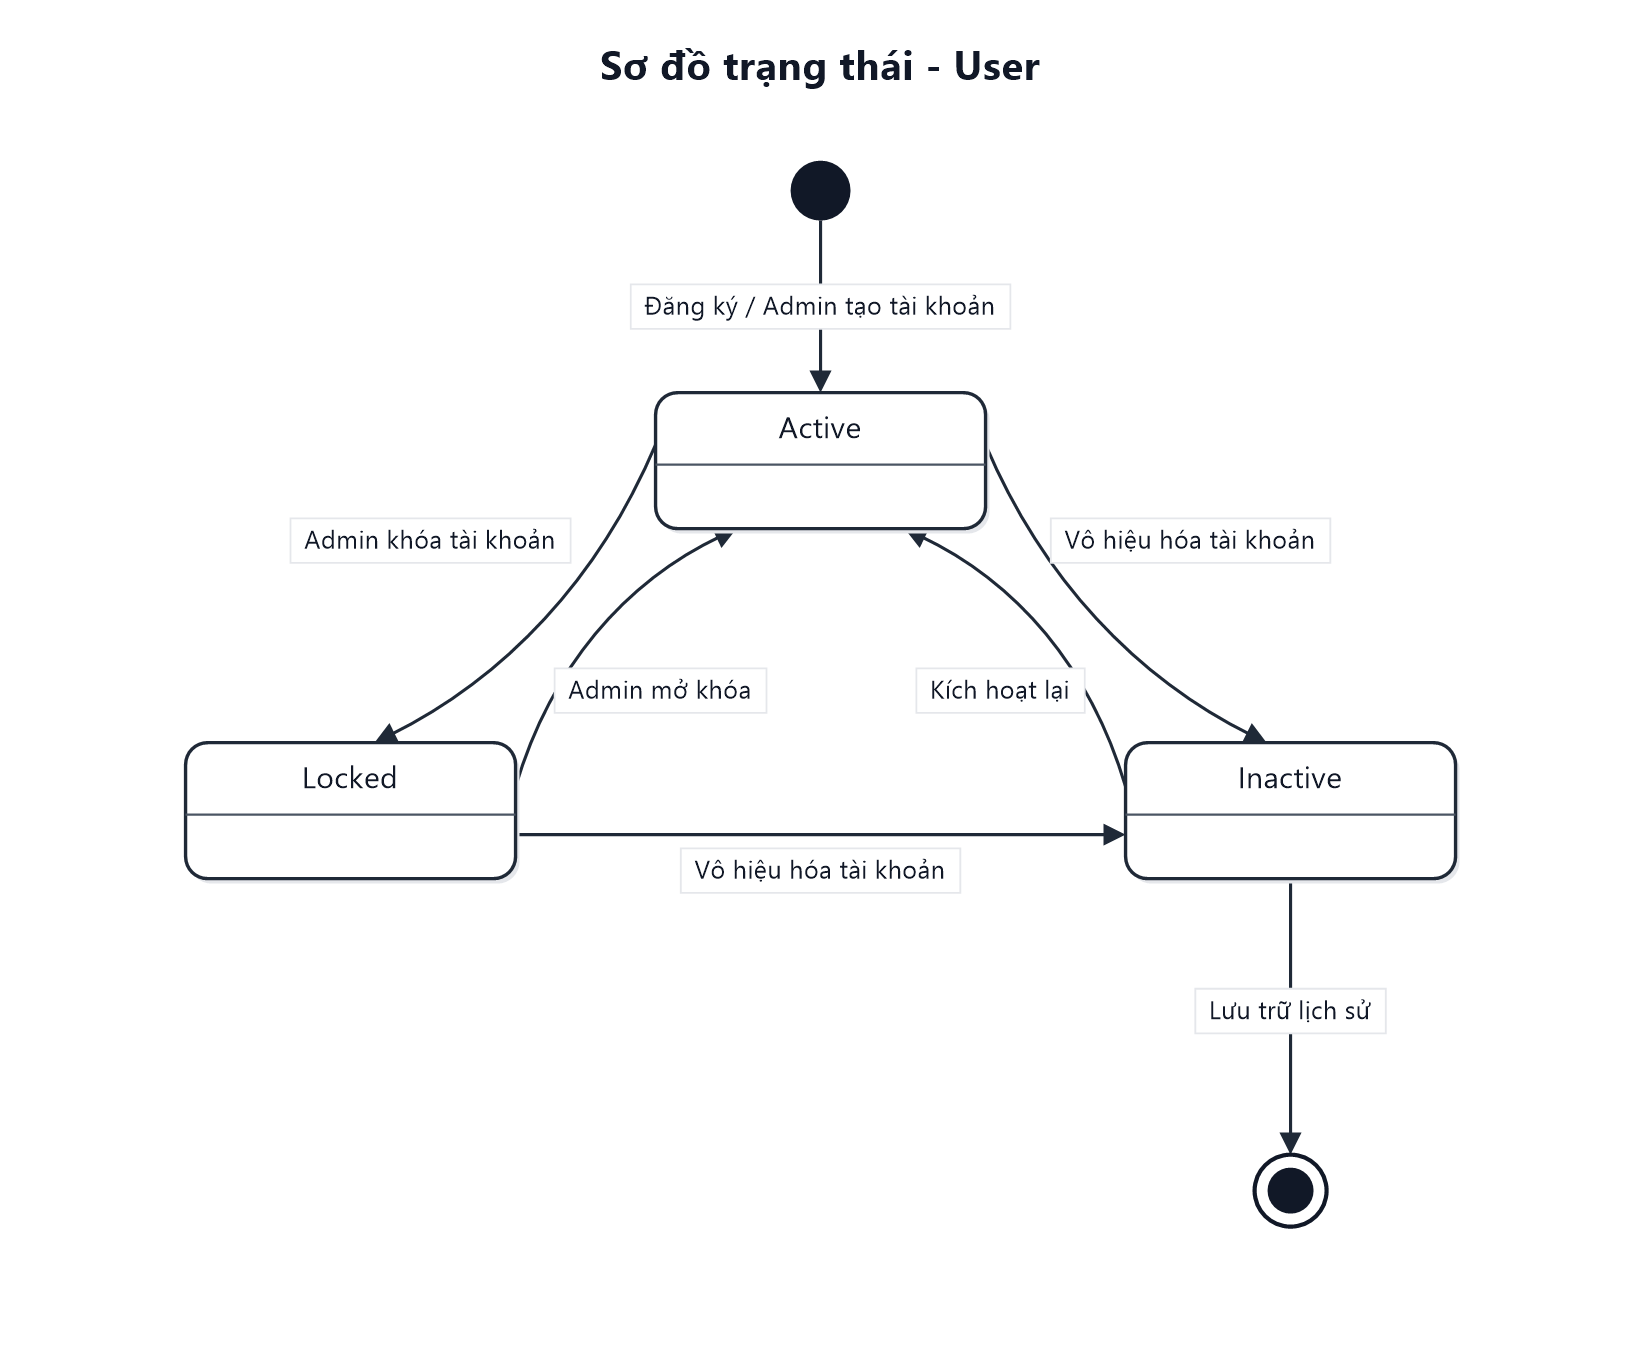
\includegraphics[width=0.82\textwidth, height=0.68\textheight, keepaspectratio]{images/state_p22_1.png}
\caption{Sơ đồ trạng thái thực thể User}
\end{figure}
\begin{itemize}
    \item \textbf{Các trạng thái:} \texttt{Active} (hoạt động bình thường ngay sau khi đăng ký hoặc được Admin tạo, \texttt{Users.Status = Active}), \texttt{Locked} (bị Admin khóa, chặn đăng nhập và token đang dùng), \texttt{Inactive} (vô hiệu hóa, có thể kích hoạt lại hoặc lưu trữ lịch sử).
    \item \textbf{Chuyển trạng thái chính:} Đăng ký / Admin tạo tài khoản $\rightarrow$ \texttt{Active}; Admin khóa/mở khóa ($\texttt{Active} \leftrightarrow \texttt{Locked}$); Vô hiệu hóa/Kích hoạt lại ($\texttt{Active/Locked} \rightarrow \texttt{Inactive} \rightarrow \texttt{Active}$).
\end{itemize}

\subsubsection{Sơ đồ trạng thái Memberships}
\begin{figure}[H]
\centering
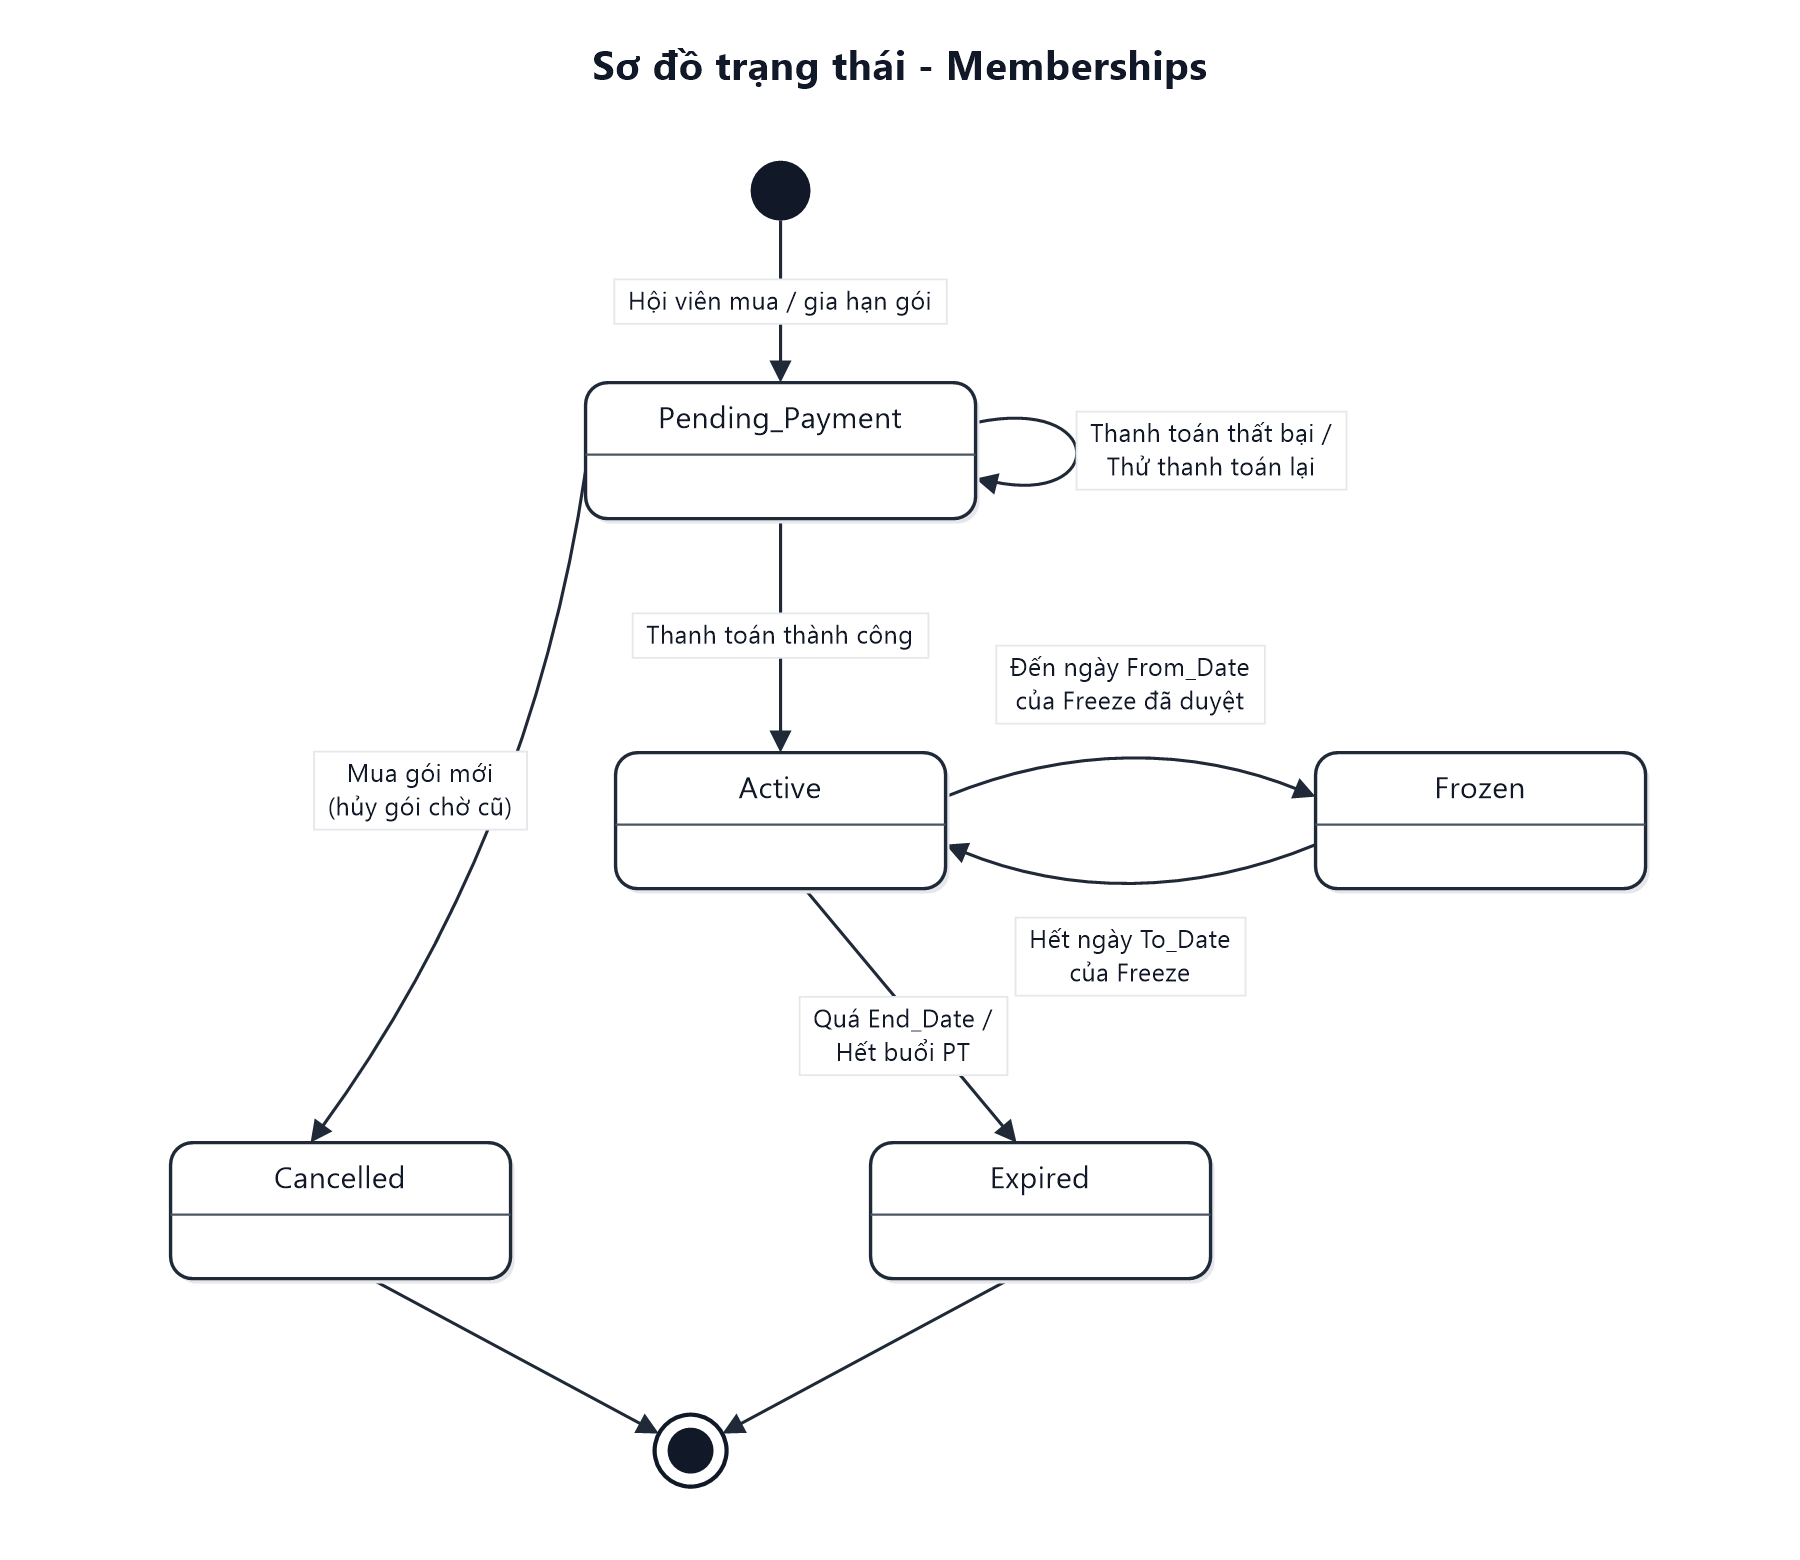
\includegraphics[width=0.82\textwidth, height=0.68\textheight, keepaspectratio]{images/state_p25_1.png}
\caption{Sơ đồ trạng thái thực thể Memberships}
\end{figure}
\begin{itemize}
    \item \textbf{Các trạng thái:} \texttt{Pending\_Payment} (chờ thanh toán), \texttt{Active} (đang hiệu lực), \texttt{Frozen} (tạm ngưng trong khoảng thời gian Freeze đã duyệt), \texttt{Expired} (hết hạn do quá \texttt{End\_Date} hoặc hết buổi PT), \texttt{Cancelled} (gói chờ cũ bị hủy khi mua lại gói mới).
    \item \textbf{Chuyển trạng thái chính:} Mua/gia hạn gói $\rightarrow$ \texttt{Pending\_Payment}; Thanh toán thành công (idempotent) $\rightarrow$ \texttt{Active}; Đến ngày \texttt{From\_Date} của Freeze đã duyệt $\rightarrow$ \texttt{Frozen} và khi hết \texttt{To\_Date} trở lại \texttt{Active}; Quá \texttt{End\_Date} hoặc hết buổi PT $\rightarrow$ \texttt{Expired}.
\end{itemize}

\subsubsection{Sơ đồ trạng thái MemberCard}
\begin{figure}[H]
\centering
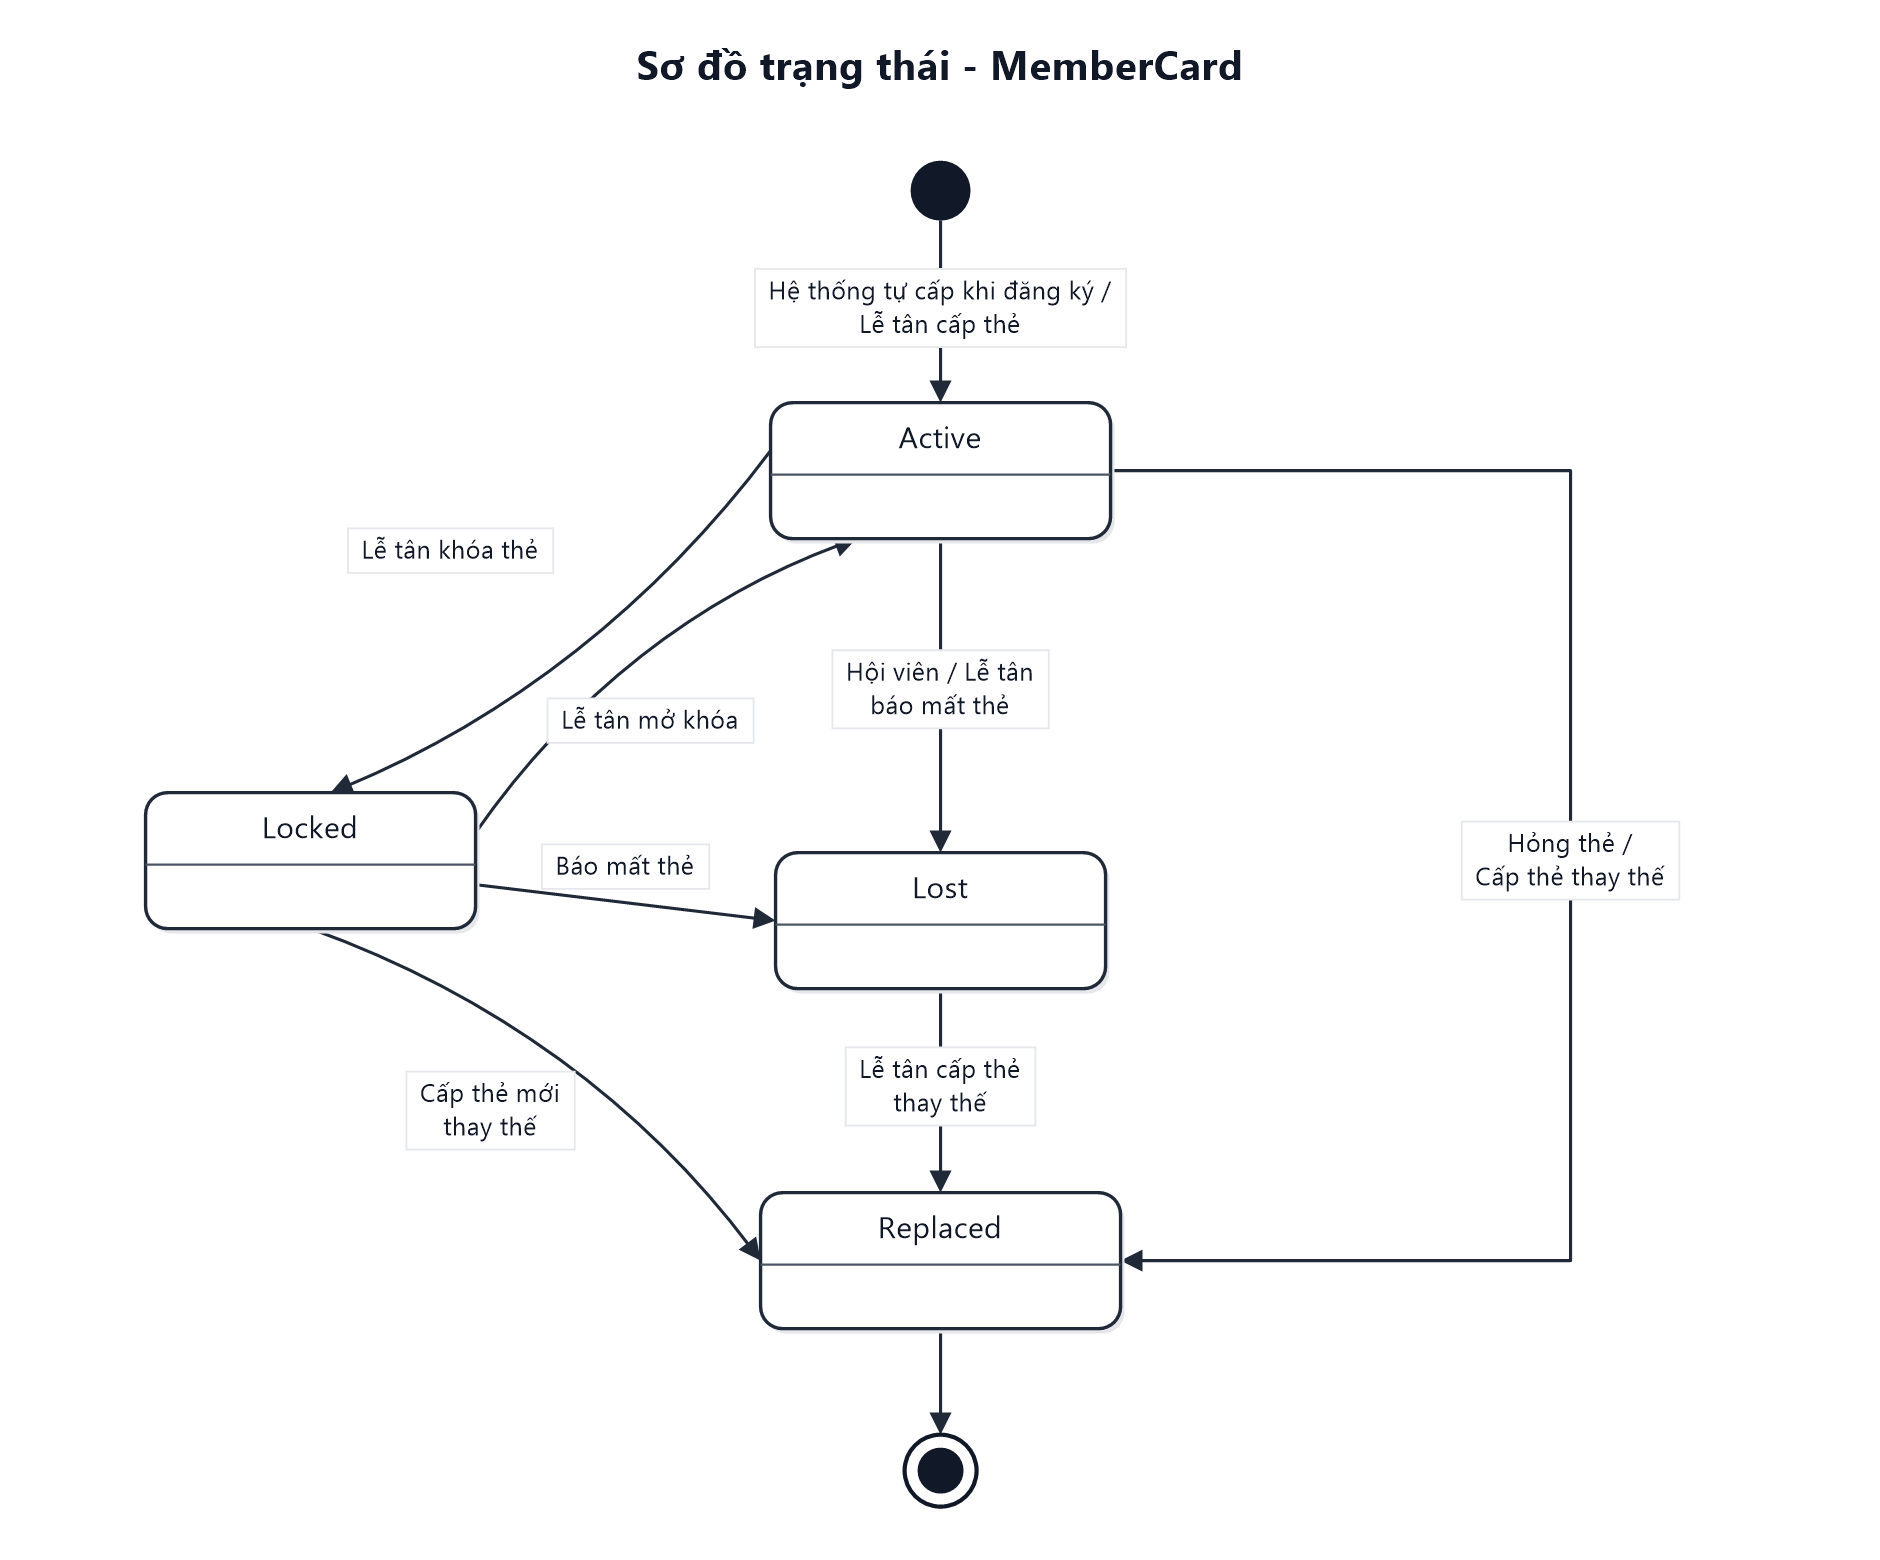
\includegraphics[width=0.82\textwidth, height=0.68\textheight, keepaspectratio]{images/state_p28_1.png}
\caption{Sơ đồ trạng thái thực thể MemberCard}
\end{figure}
\begin{itemize}
    \item \textbf{Các trạng thái:} \texttt{Active} (thẻ hợp lệ -- hệ thống tự cấp khi hội viên đăng ký hoặc Lễ tân cấp mới), \texttt{Locked} (thẻ tạm khóa, quét QR bị từ chối nhưng có thể được Lễ tân mở khóa lại về \texttt{Active}), \texttt{Lost} (thẻ đã báo mất -- vô hiệu hóa vĩnh viễn không thể mở khóa lại, chỉ hỗ trợ check-in thủ công và chờ cấp thẻ mới), \texttt{Replaced} (thẻ cũ đã được thay thế bằng thẻ mới).
\end{itemize}

\subsubsection{Sơ đồ trạng thái Booking}
\begin{figure}[H]
\centering
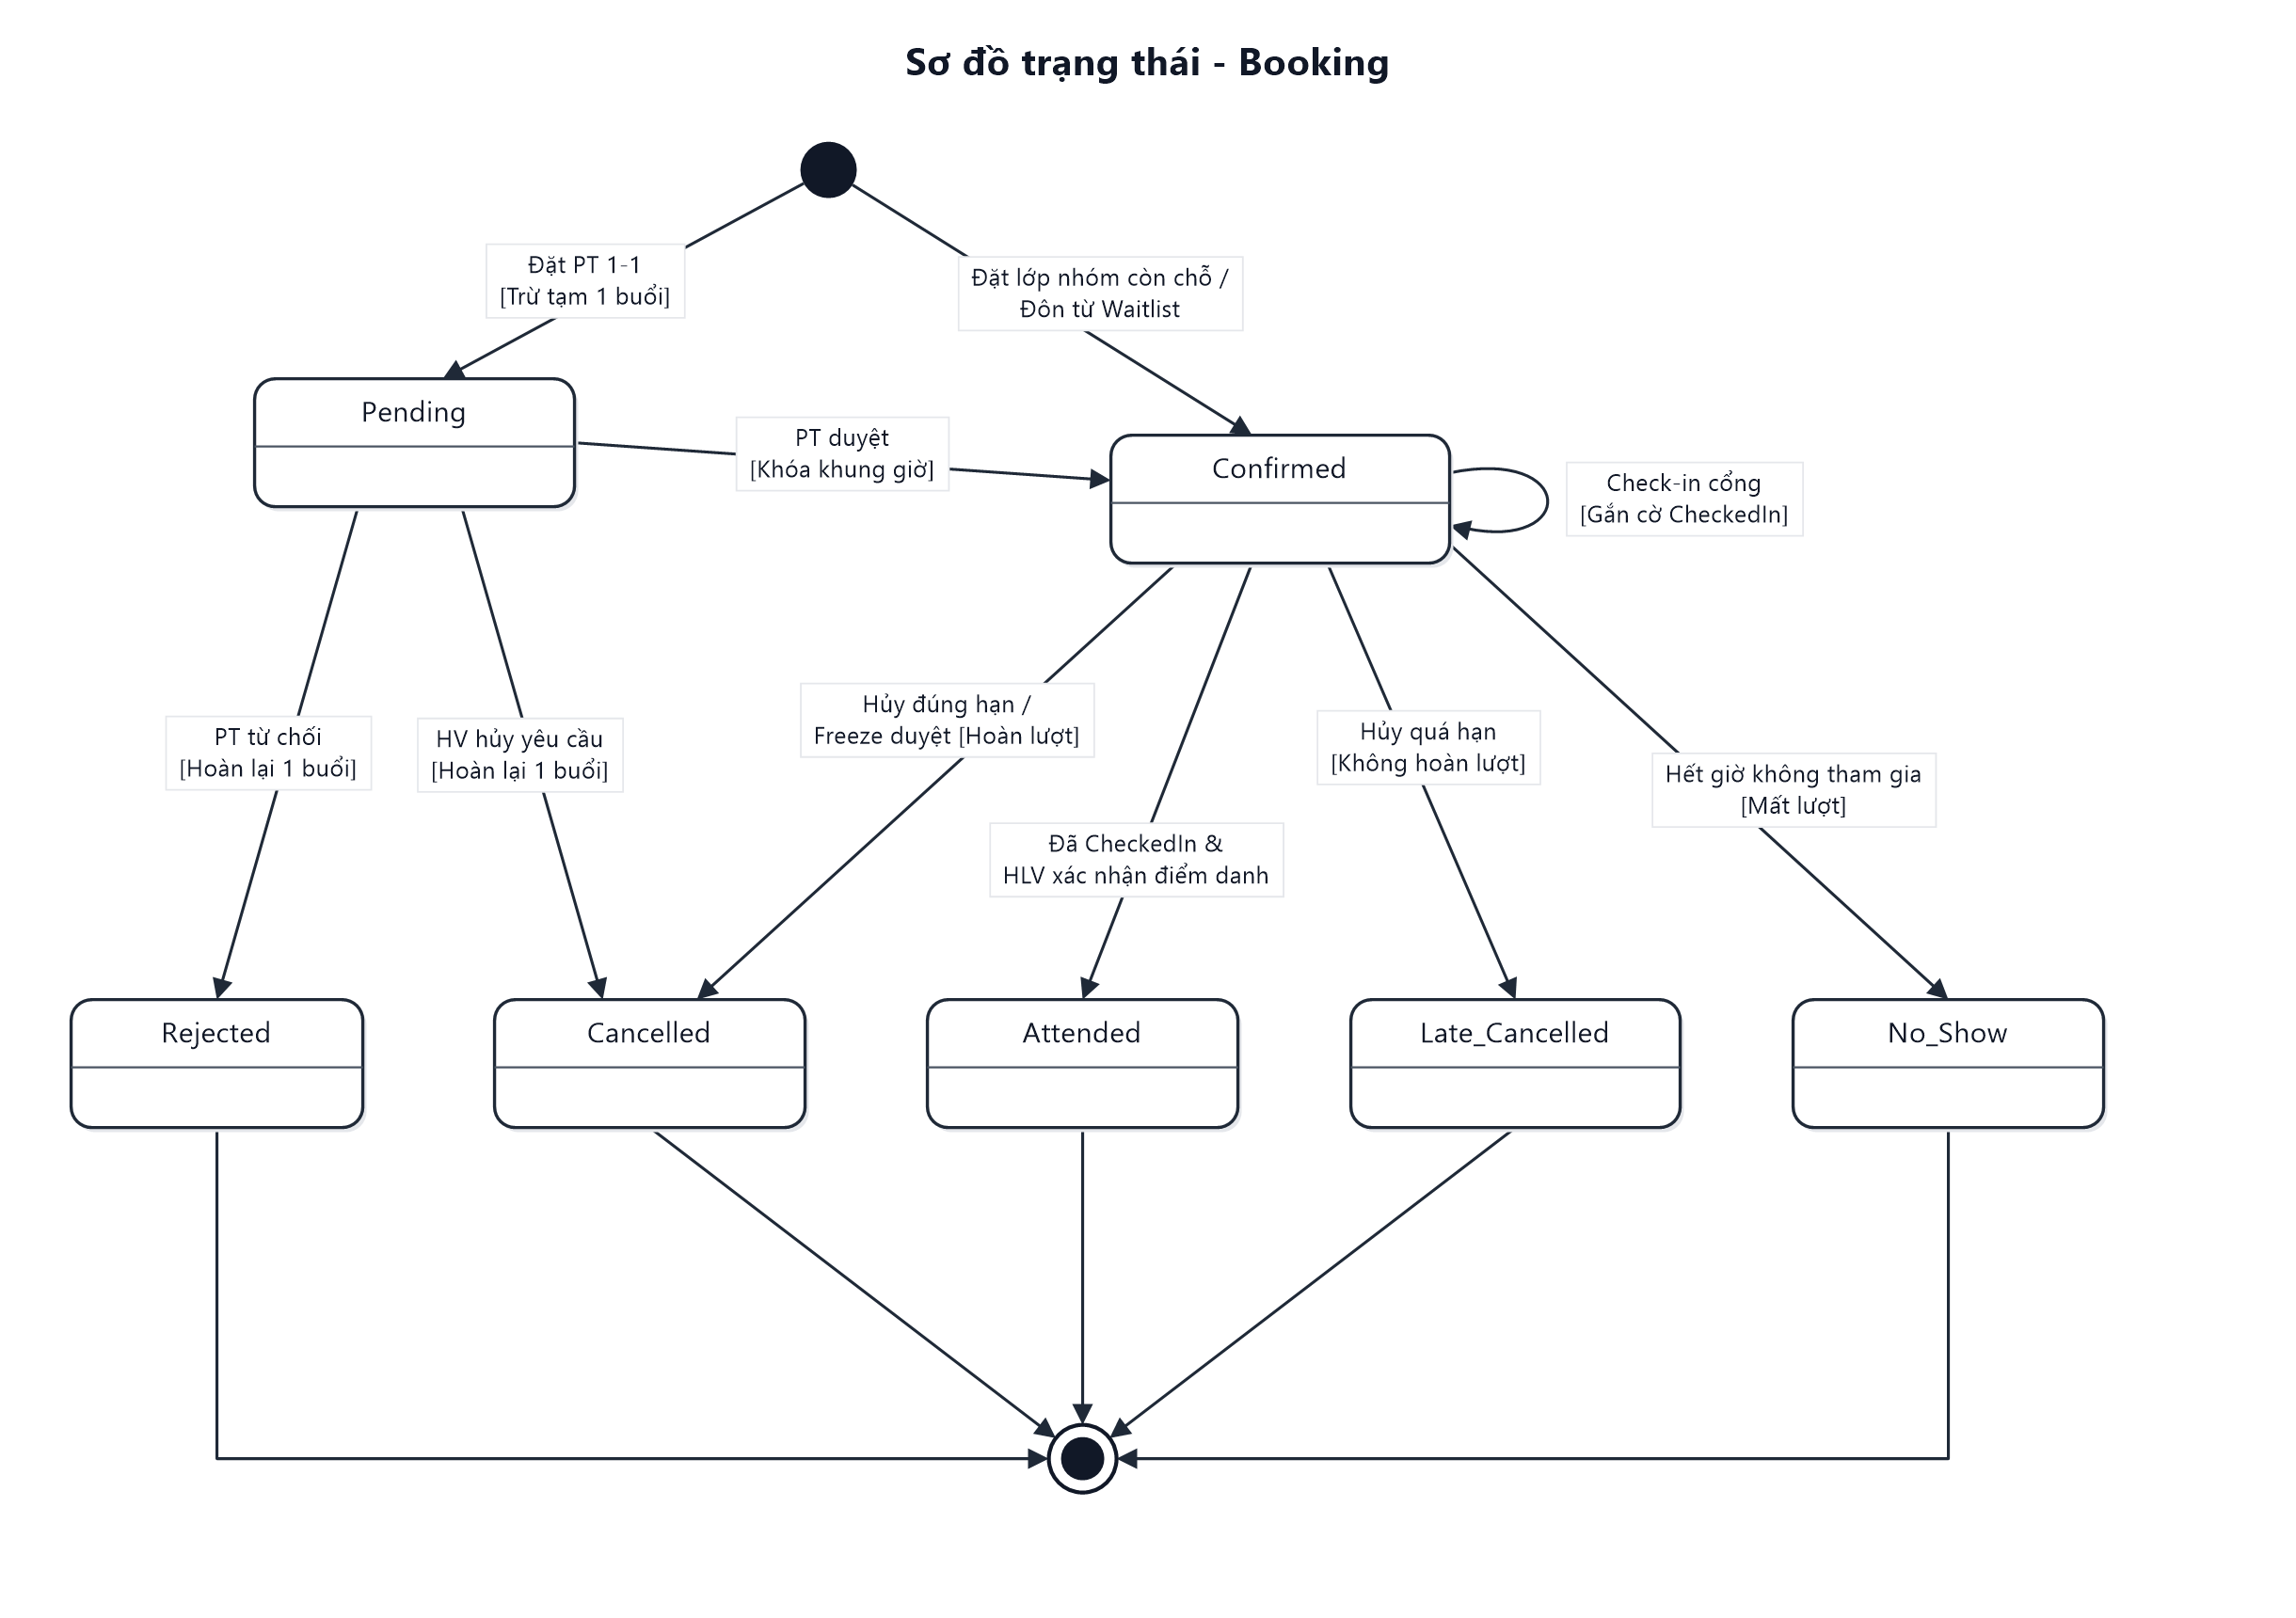
\includegraphics[width=0.82\textwidth, height=0.68\textheight, keepaspectratio]{images/state_p30_1.png}
\caption{Sơ đồ trạng thái thực thể Booking}
\end{figure}
\begin{itemize}
    \item \textbf{Các trạng thái:} \texttt{Pending} (chờ PT duyệt đối với lịch PT 1-kèm-1, hệ thống trừ tạm 1 buổi ngay khi gửi yêu cầu), \texttt{Confirmed} (đã xác nhận đối với lớp nhóm còn chỗ, đôn từ hàng chờ \texttt{Waitlist\_Entry} hoặc PT đã duyệt và khóa khung giờ; khi hội viên check-in cổng, hệ thống gắn cờ \texttt{CheckedIn}), \texttt{Attended} (đã check-in tại chi nhánh và được HLV xác nhận điểm danh / hoàn thành buổi tập), \texttt{Cancelled} (hủy đúng hạn, HV hủy yêu cầu chờ duyệt hoặc tự hủy khi Freeze duyệt -- hoàn lại lượt), \texttt{Late\_Cancelled} (hủy quá hạn -- không hoàn lượt), \texttt{Rejected} (PT từ chối -- hoàn lại 1 buổi tạm giữ), \texttt{No\_Show} (hết giờ không tham gia -- mất lượt). Riêng trạng thái hàng chờ lớp được tách quản lý độc lập ở thực thể \texttt{Waitlist\_Entry}.
\end{itemize}

\subsubsection{Sơ đồ trạng thái Waitlist\_Entry}
\begin{figure}[H]
\centering
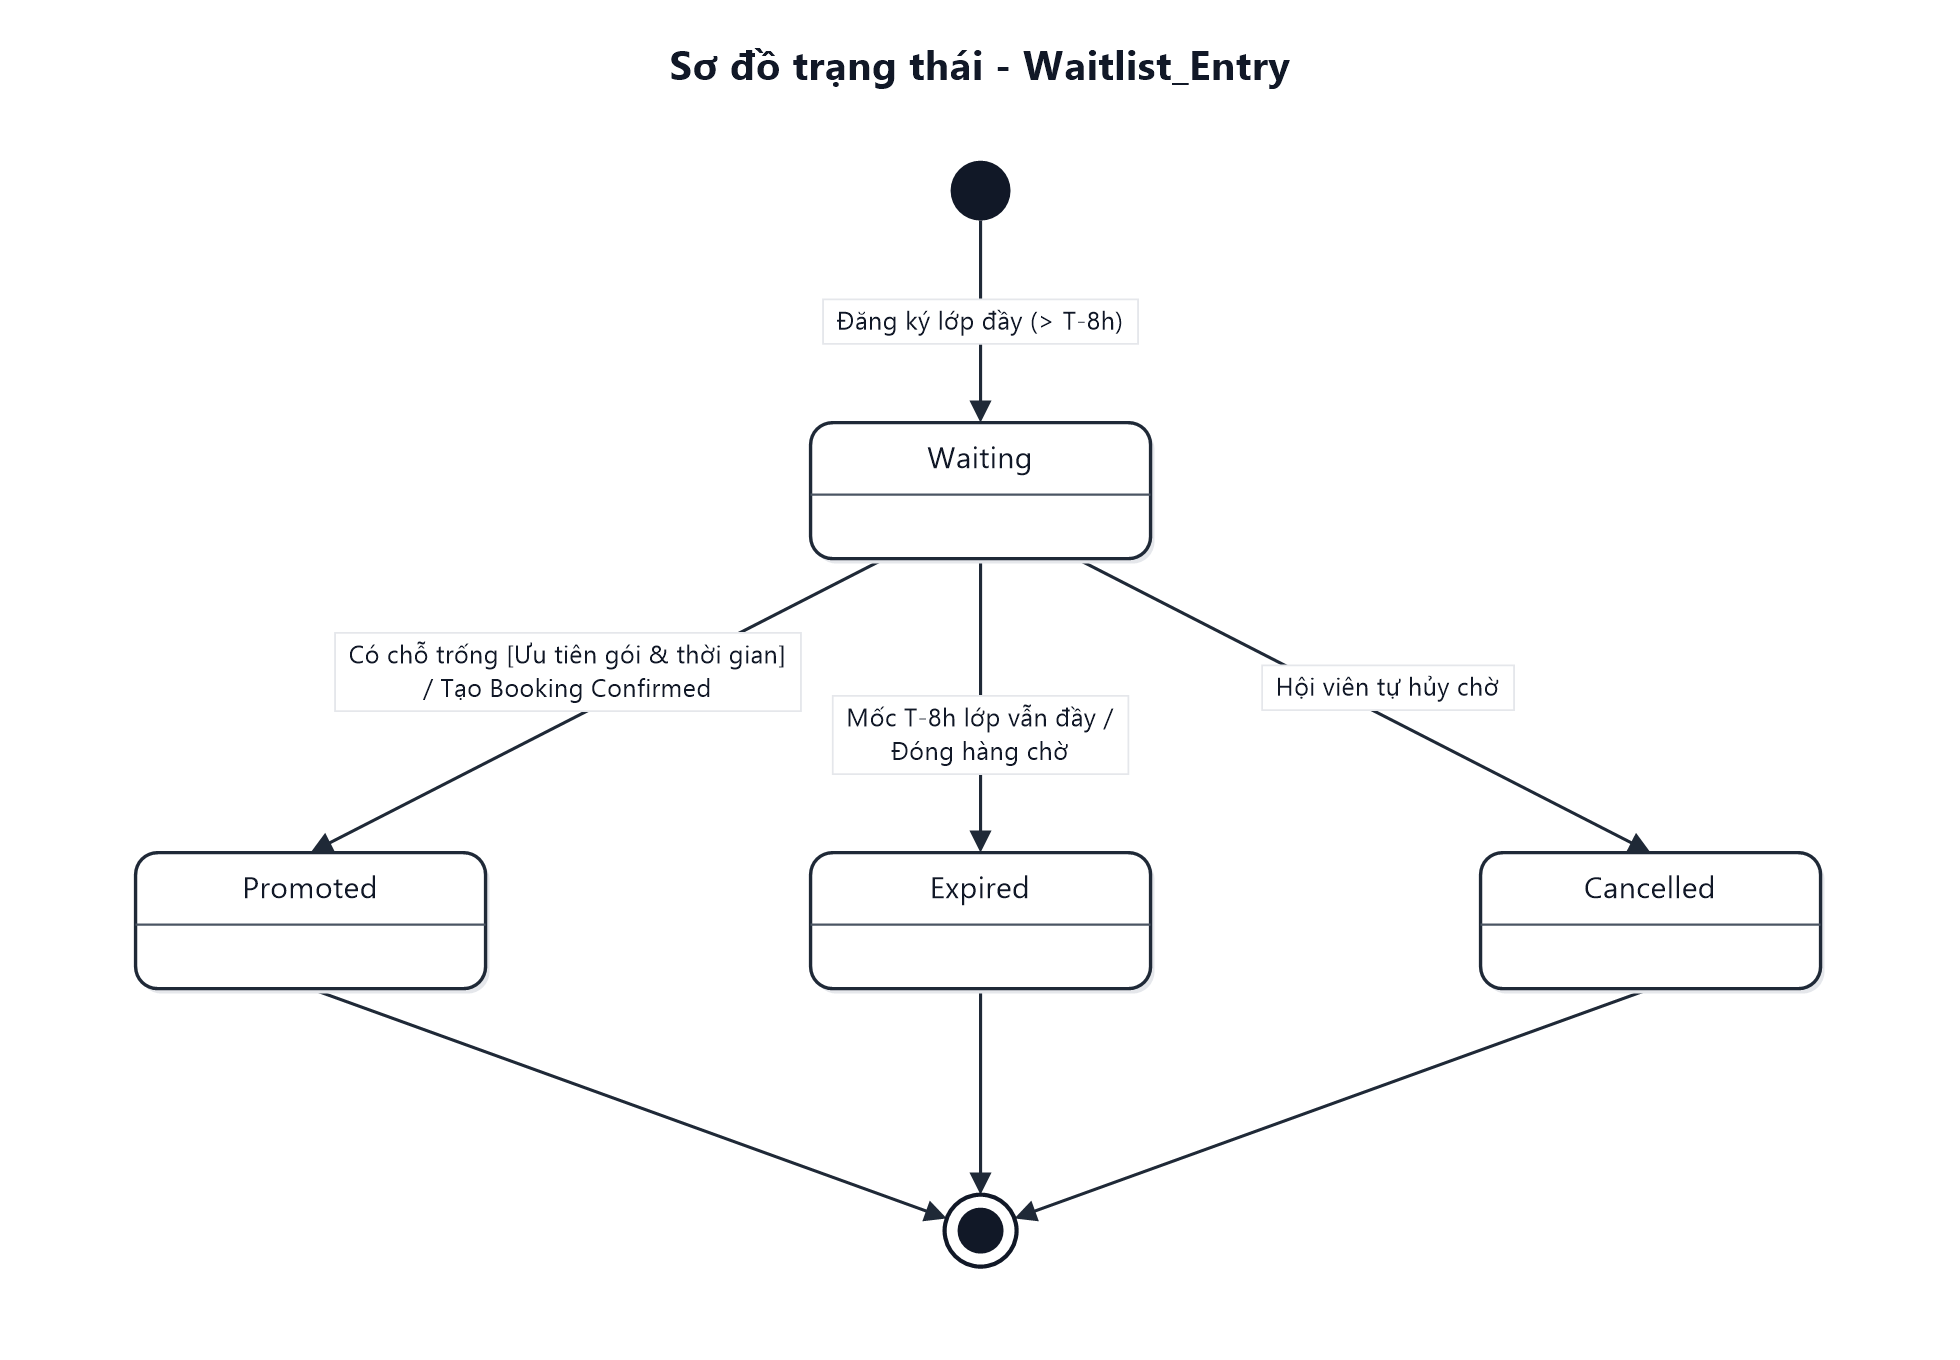
\includegraphics[width=0.82\textwidth, height=0.68\textheight, keepaspectratio]{images/state_p33_1.png}
\caption{Sơ đồ trạng thái thực thể Waitlist\_Entry}
\end{figure}
\begin{itemize}
    \item \textbf{Các trạng thái:} \texttt{Waiting} (đang chờ xếp theo \texttt{Priority\_Level} và thời gian đăng ký), \texttt{Promoted} (được đôn lên \texttt{Confirmed} khi có chỗ trống), \texttt{Expired} (tự động đóng tại mốc $T-8h$ nếu lớp vẫn đầy), \texttt{Cancelled} (hội viên tự hủy chờ).
\end{itemize}

\subsubsection{Sơ đồ trạng thái FreezeRequest}
\begin{figure}[H]
\centering
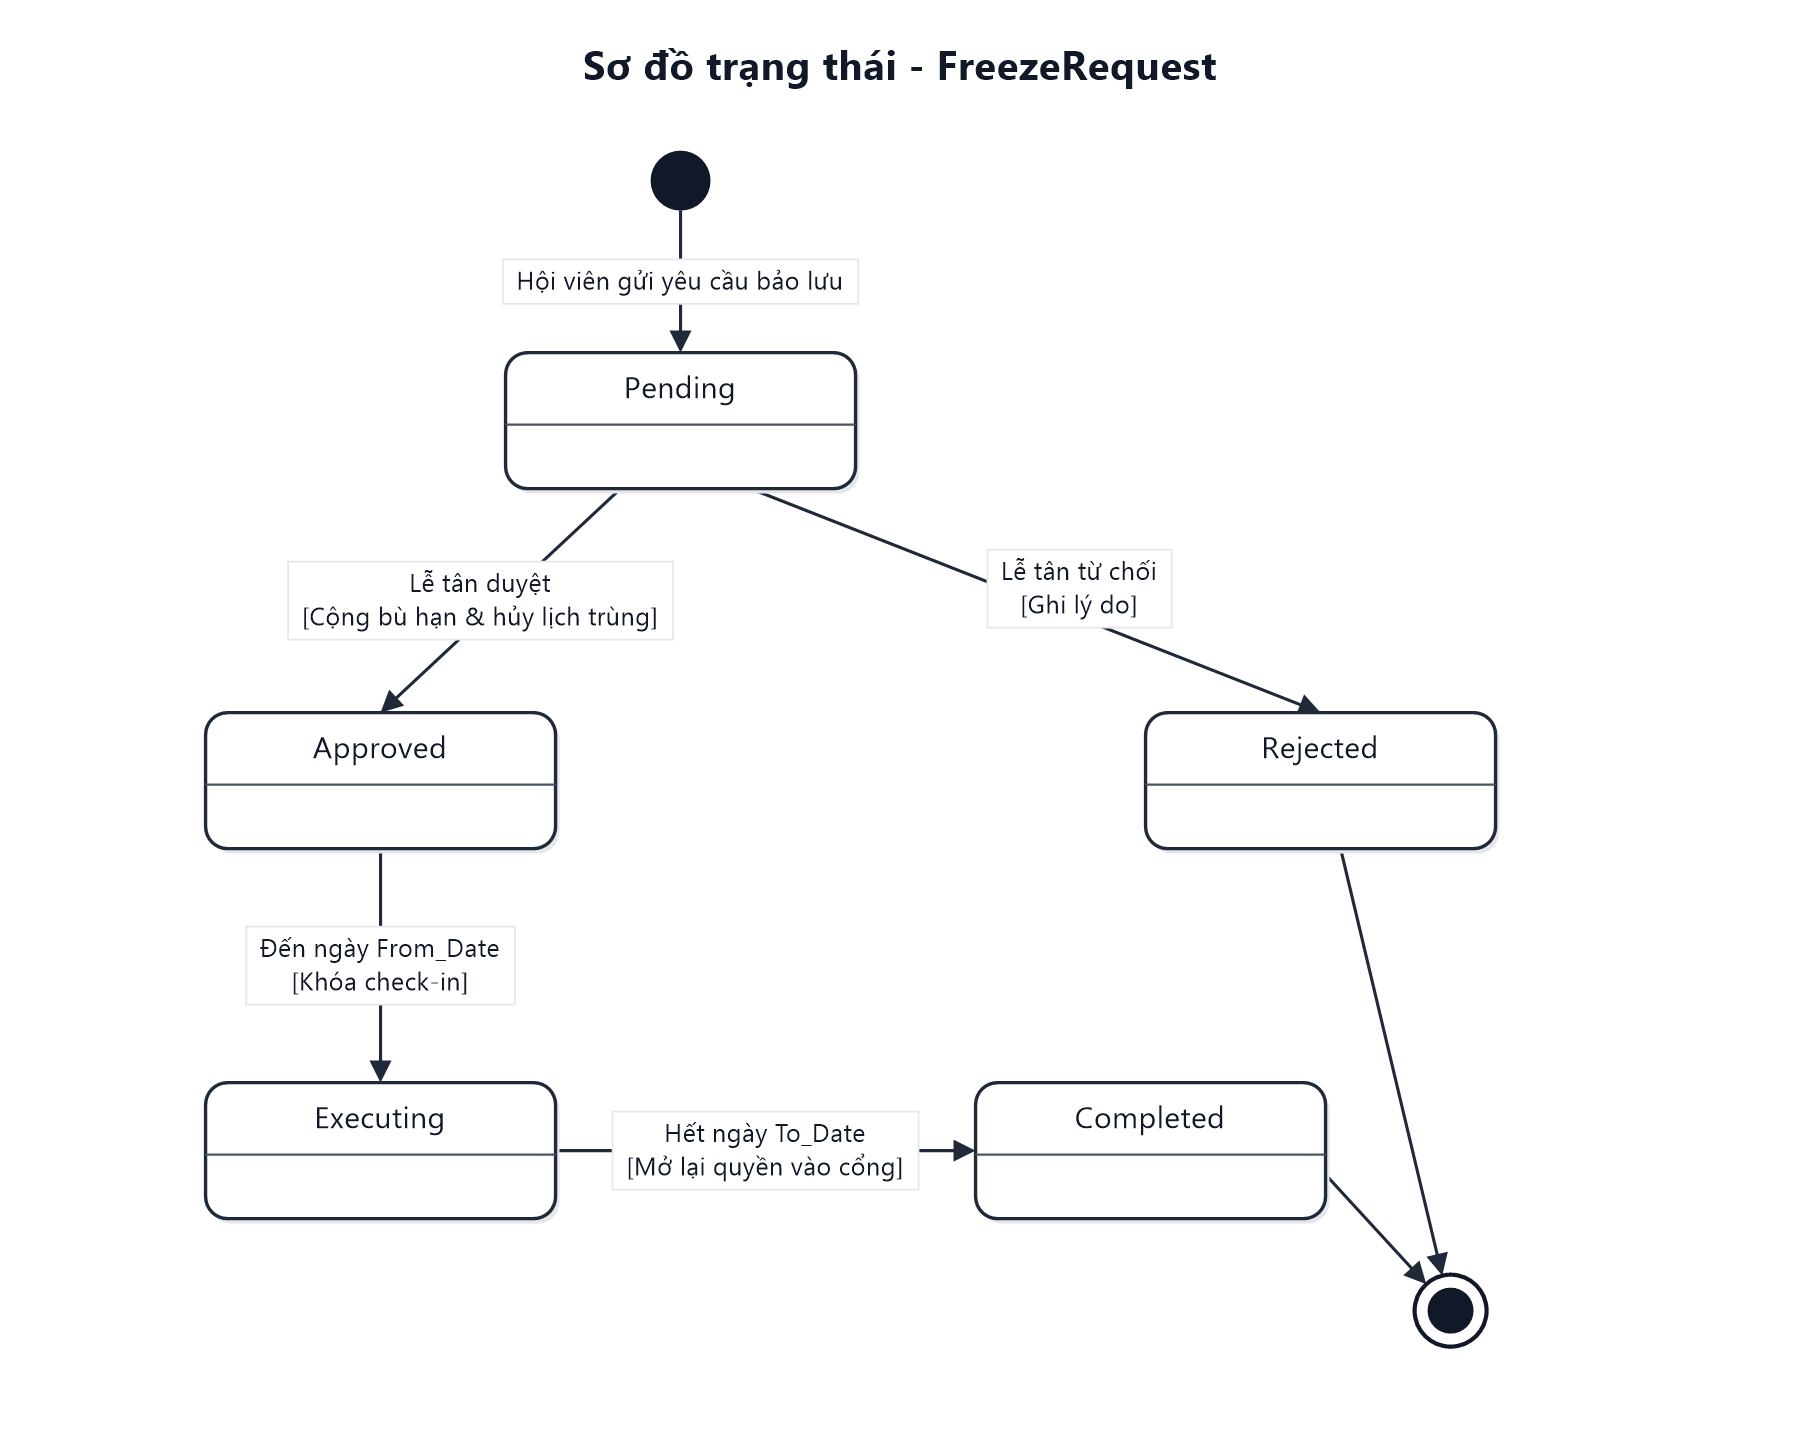
\includegraphics[width=0.82\textwidth, height=0.68\textheight, keepaspectratio]{images/state_p35_1.png}
\caption{Sơ đồ trạng thái thực thể FreezeRequest}
\end{figure}
\begin{itemize}
    \item \textbf{Các trạng thái:} \texttt{Pending} (chờ Lễ tân xét duyệt), \texttt{Approved} (Lễ tân duyệt -- hệ thống cộng bù \texttt{End\_Date}, dời gói gia hạn nối tiếp và tự động hủy các lịch tập trùng trong khoảng bảo lưu), \texttt{Rejected} (Lễ tân từ chối kèm lý do), \texttt{Executing} (đến ngày \texttt{From\_Date}, khóa quyền check-in tại cổng), \texttt{Completed} (hết ngày \texttt{To\_Date}, mở lại quyền vào cổng).
\end{itemize}

\subsubsection{Sơ đồ trạng thái ClassSession}
\begin{figure}[H]
\centering
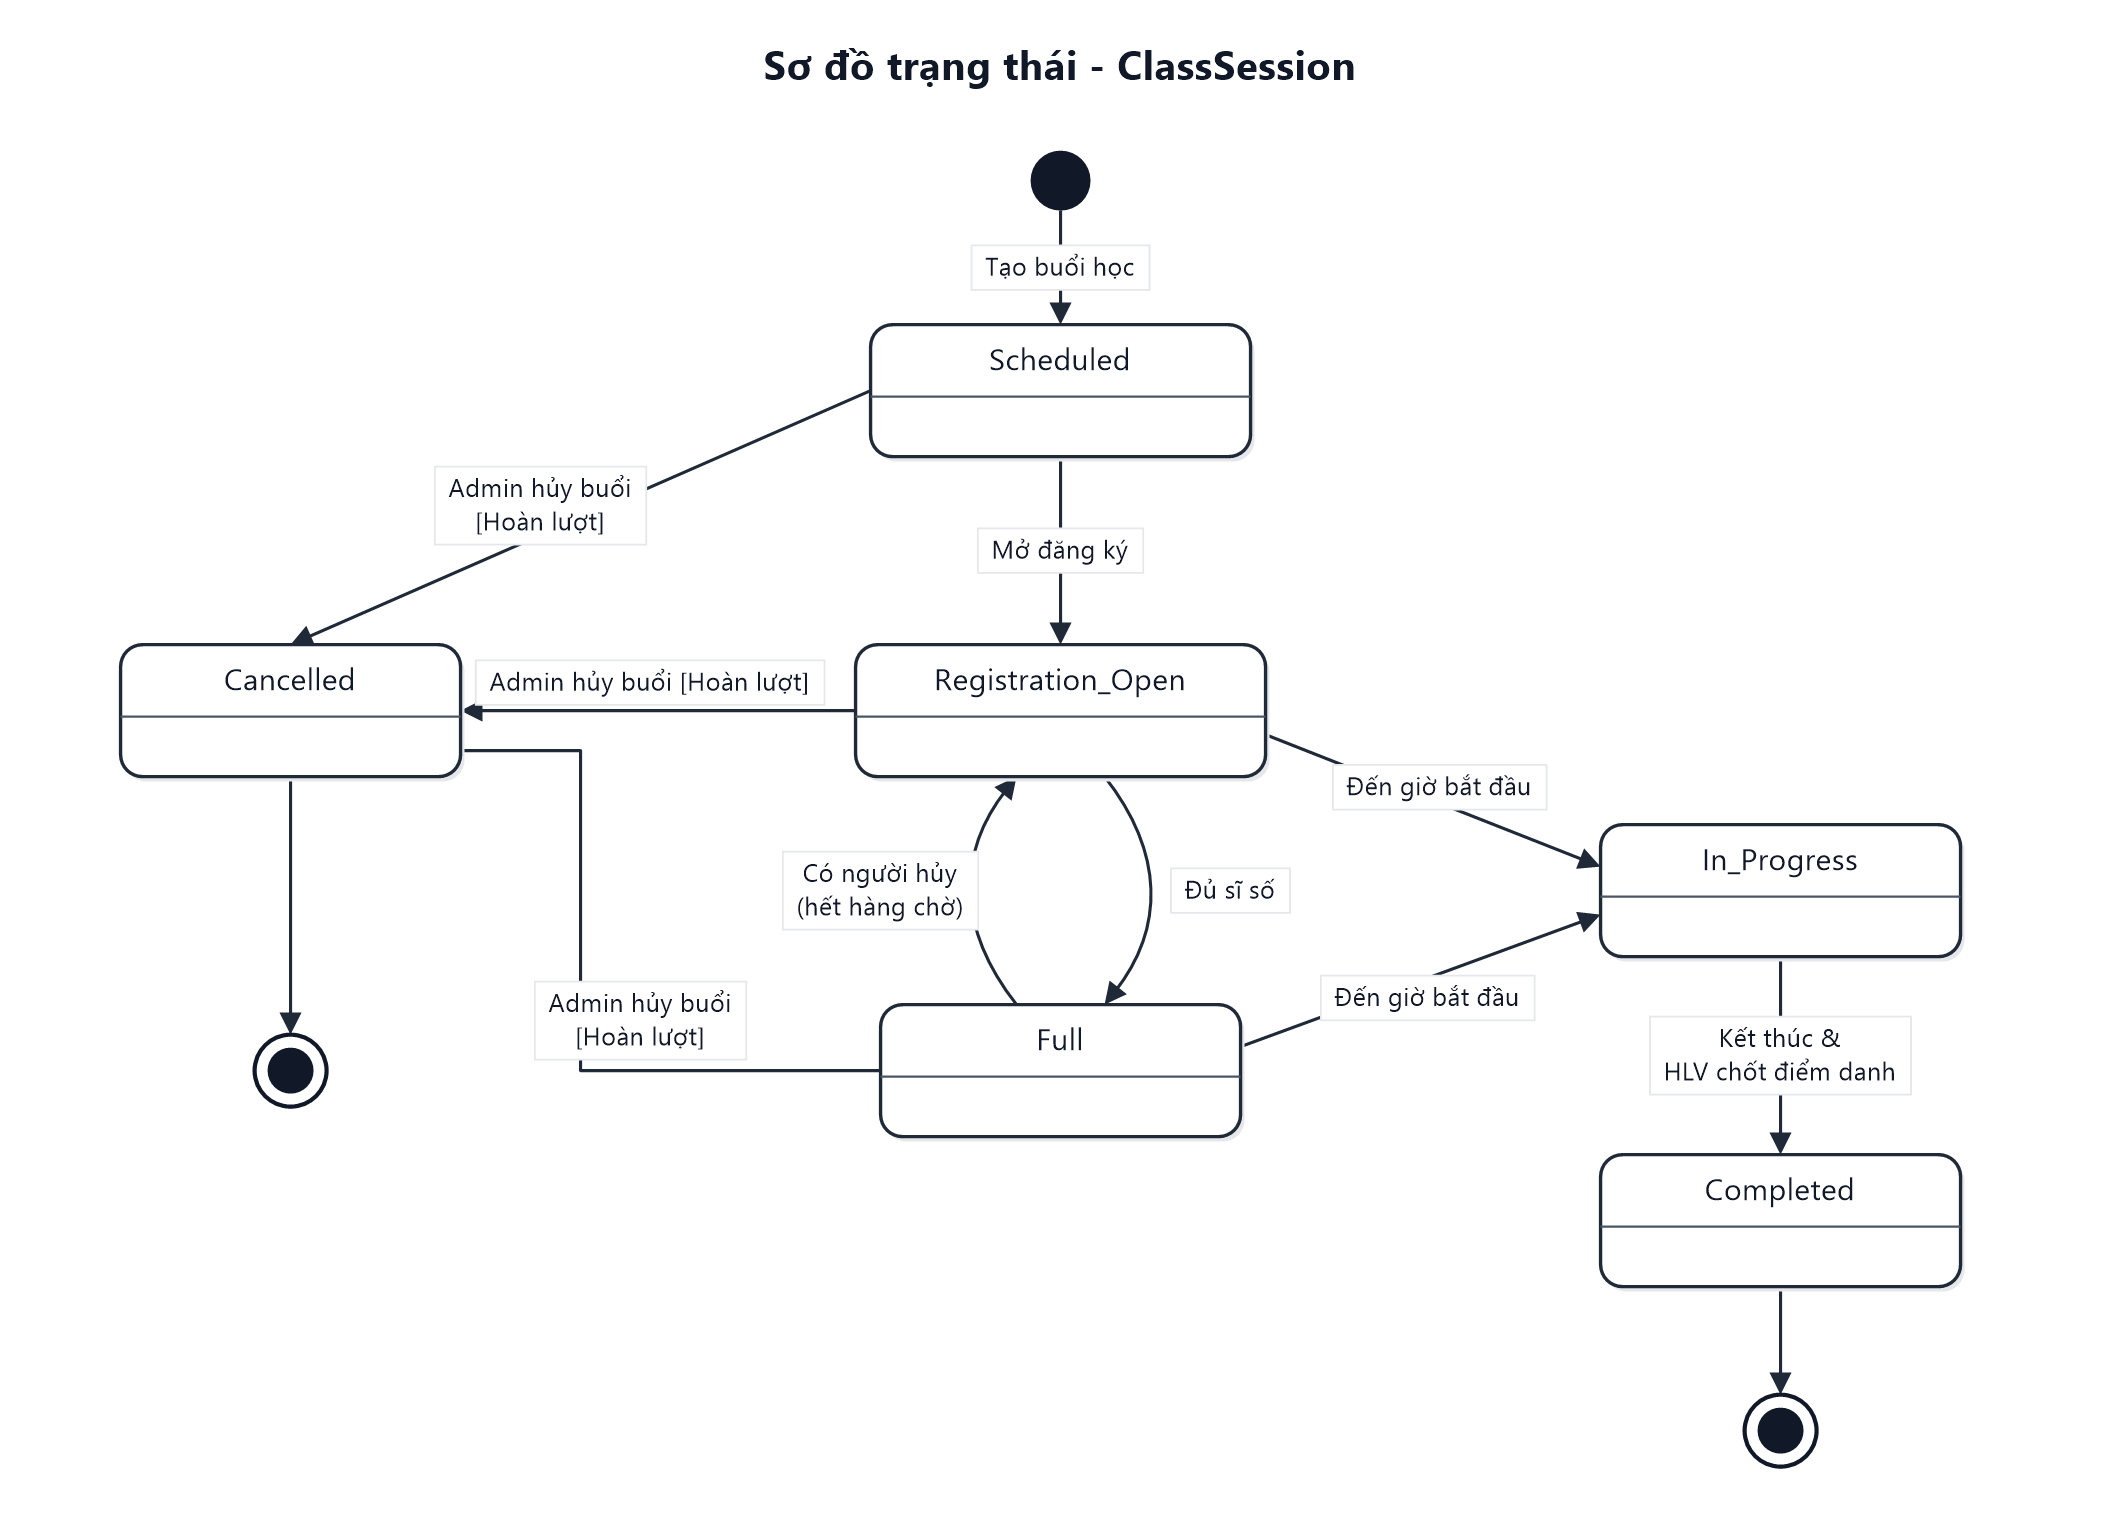
\includegraphics[width=0.82\textwidth, height=0.68\textheight, keepaspectratio]{images/state_p37_1.png}
\caption{Sơ đồ trạng thái thực thể ClassSession}
\end{figure}
\begin{itemize}
    \item \textbf{Các trạng thái:} \texttt{Scheduled} (đã lên lịch), \texttt{Registration\_Open} (đang mở đăng ký), \texttt{Full} (đủ sĩ số, chuyển về \texttt{Registration\_Open} nếu có người hủy), \texttt{In\_Progress} (đang diễn ra, cho phép điểm danh), \texttt{Completed} (hoàn tất, mở quyền đánh giá), \texttt{Cancelled} (Admin hủy buổi, hoàn lượt cho hội viên).
\end{itemize}

\subsubsection{Sơ đồ trạng thái GymClass}
\begin{figure}[H]
\centering
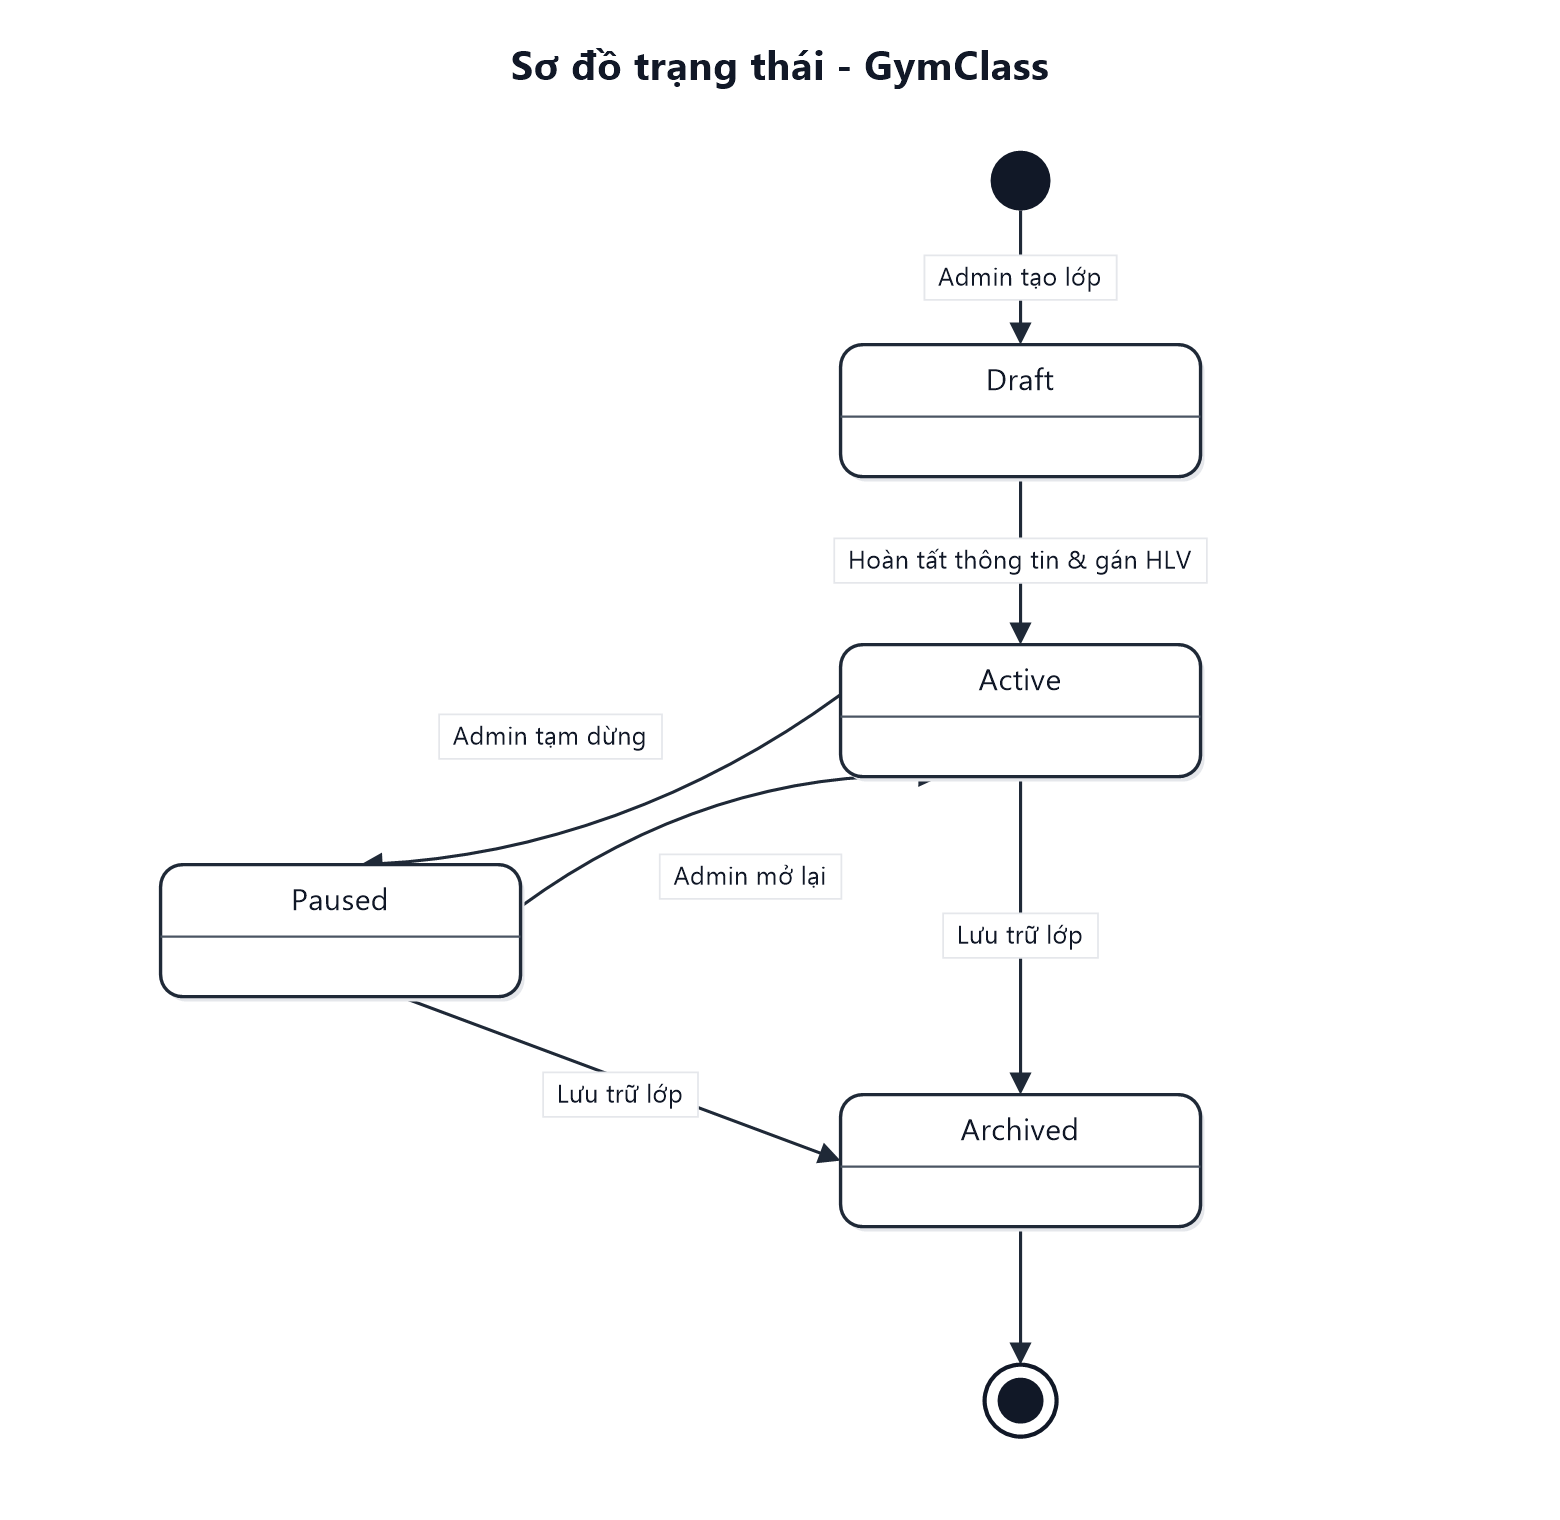
\includegraphics[width=0.82\textwidth, height=0.68\textheight, keepaspectratio]{images/state_p39_1.png}
\caption{Sơ đồ trạng thái thực thể GymClass}
\end{figure}
\begin{itemize}
    \item \textbf{Các trạng thái:} \texttt{Draft} (bản nháp đang soạn), \texttt{Active} (đã gán HLV, cho phép sinh buổi học và đăng ký), \texttt{Paused} (tạm dừng mở lớp mới, có thể mở lại), \texttt{Archived} (đã lưu trữ, chỉ tra cứu lịch sử).
\end{itemize}

\subsubsection{Sơ đồ trạng thái Checkin}
\begin{figure}[H]
\centering
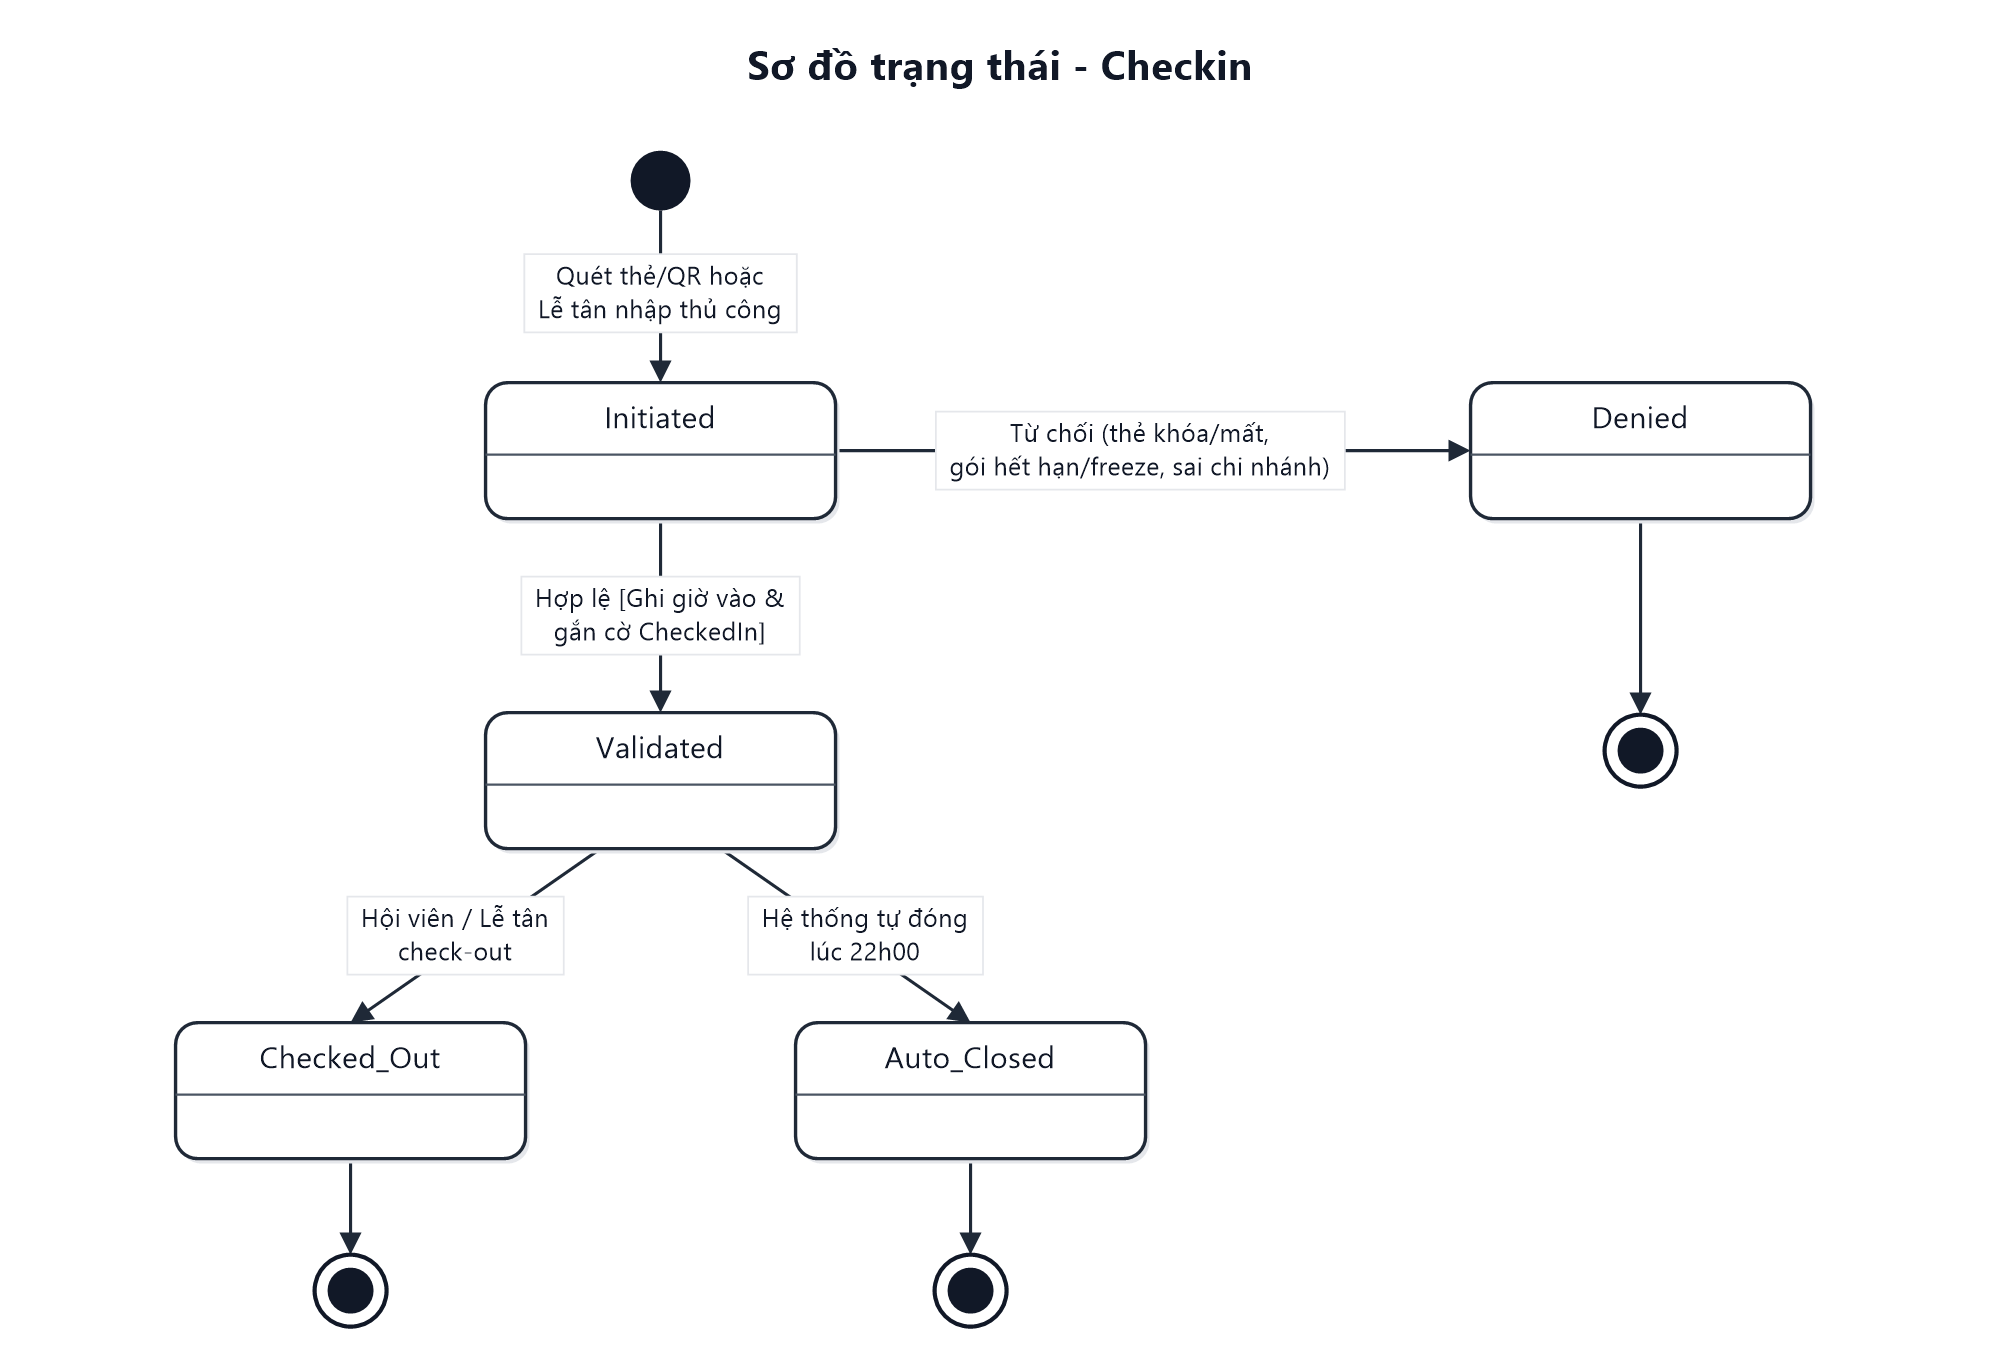
\includegraphics[width=0.82\textwidth, height=0.68\textheight, keepaspectratio]{images/state_p41_1.png}
\caption{Sơ đồ trạng thái thực thể Checkin}
\end{figure}
\begin{itemize}
    \item \textbf{Các trạng thái:} \texttt{Initiated} (bắt đầu quét thẻ/QR hoặc Lễ tân nhập thủ công để kiểm tra điều kiện), \texttt{Denied} (từ chối vào cổng do thẻ \texttt{Locked/Lost}, gói hết hạn/freeze hoặc sai chi nhánh và lưu nhật ký lý do), \texttt{Validated} (kiểm tra hợp lệ, mở cổng, ghi giờ vào và tự động gắn cờ \texttt{CheckedIn} cho các lịch lớp/PT trong ngày), \texttt{Checked\_Out} (hội viên hoặc Lễ tân check-out), \texttt{Auto\_Closed} (hệ thống tự động check-out lúc 22h00 đóng cửa).
\end{itemize}

\subsubsection{Sơ đồ trạng thái Payment}
\begin{figure}[H]
\centering
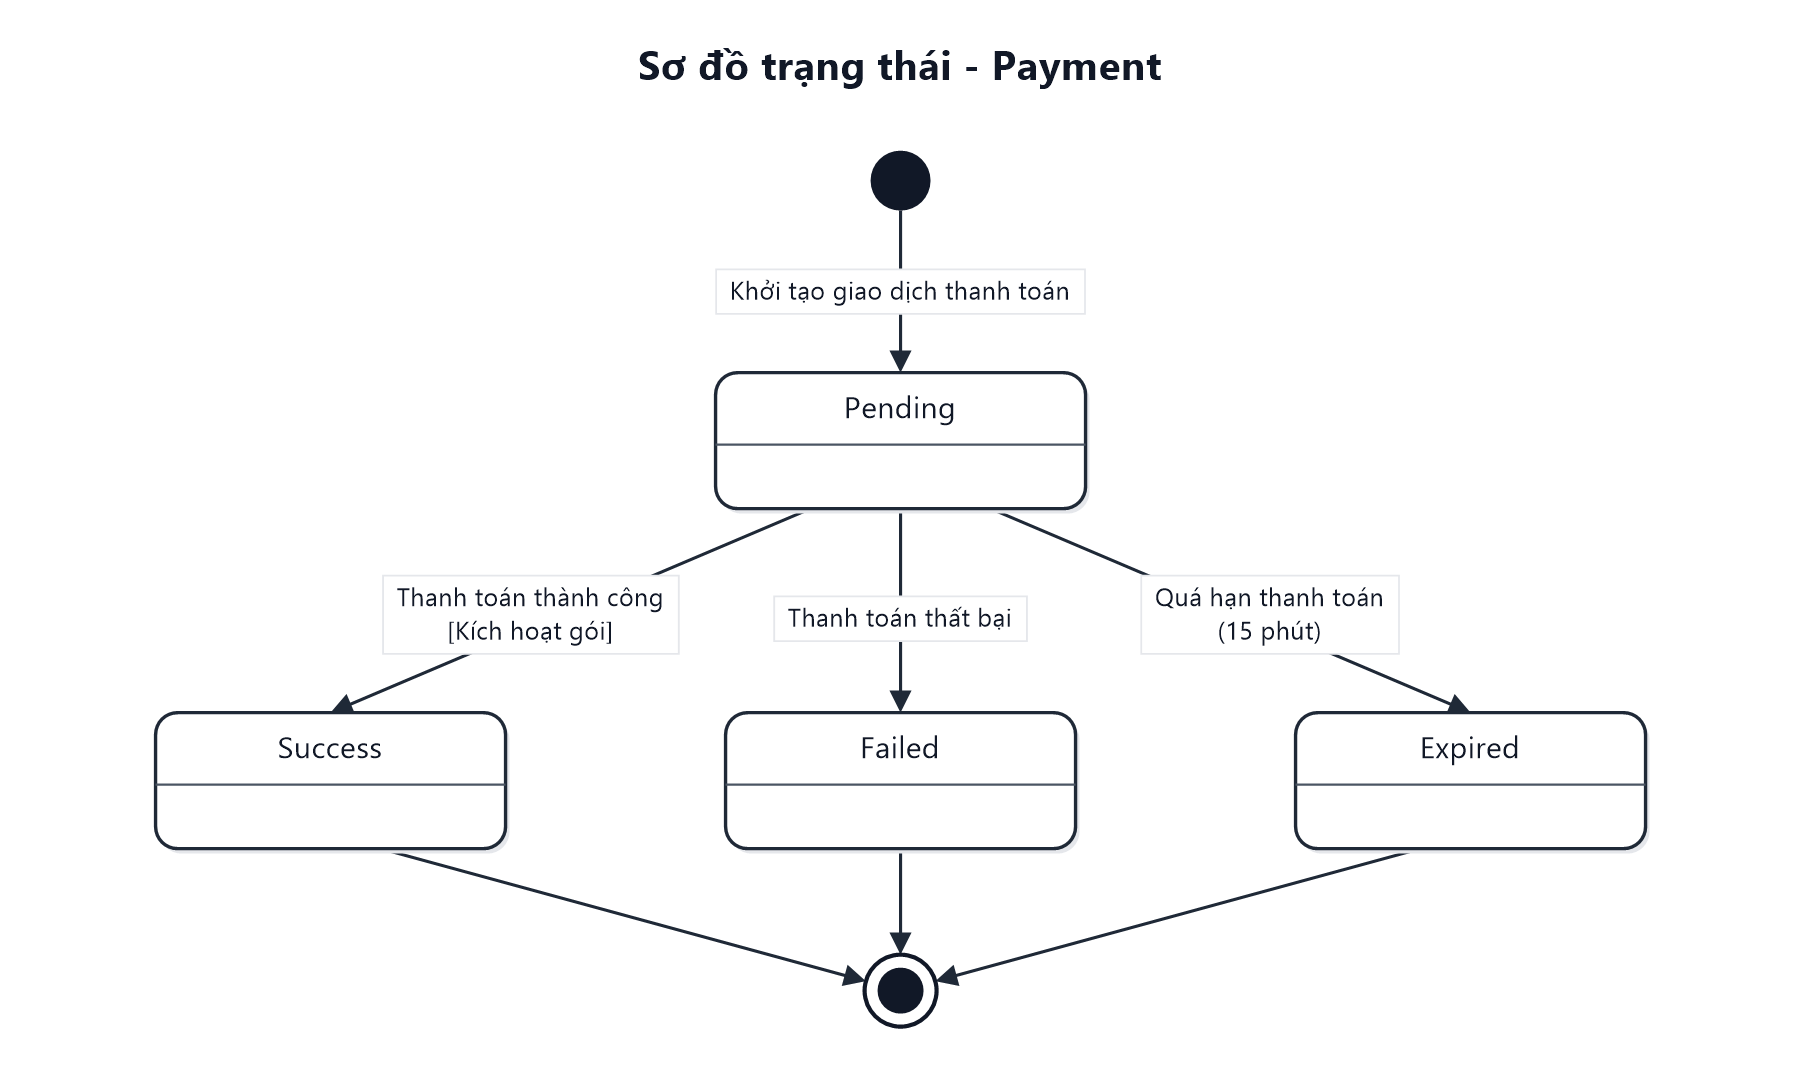
\includegraphics[width=0.82\textwidth, height=0.68\textheight, keepaspectratio]{images/state_p43_1.png}
\caption{Sơ đồ trạng thái thực thể Payment}
\end{figure}
\begin{itemize}
    \item \textbf{Các trạng thái:} \texttt{Pending} (chờ thanh toán), \texttt{Success} (thanh toán thành công, kích hoạt gói và kết thúc giao dịch), \texttt{Failed} (thanh toán thất bại), \texttt{Expired} (quá hạn 15 phút).
\end{itemize}

\subsubsection{Sơ đồ trạng thái Notification}
\begin{figure}[H]
\centering
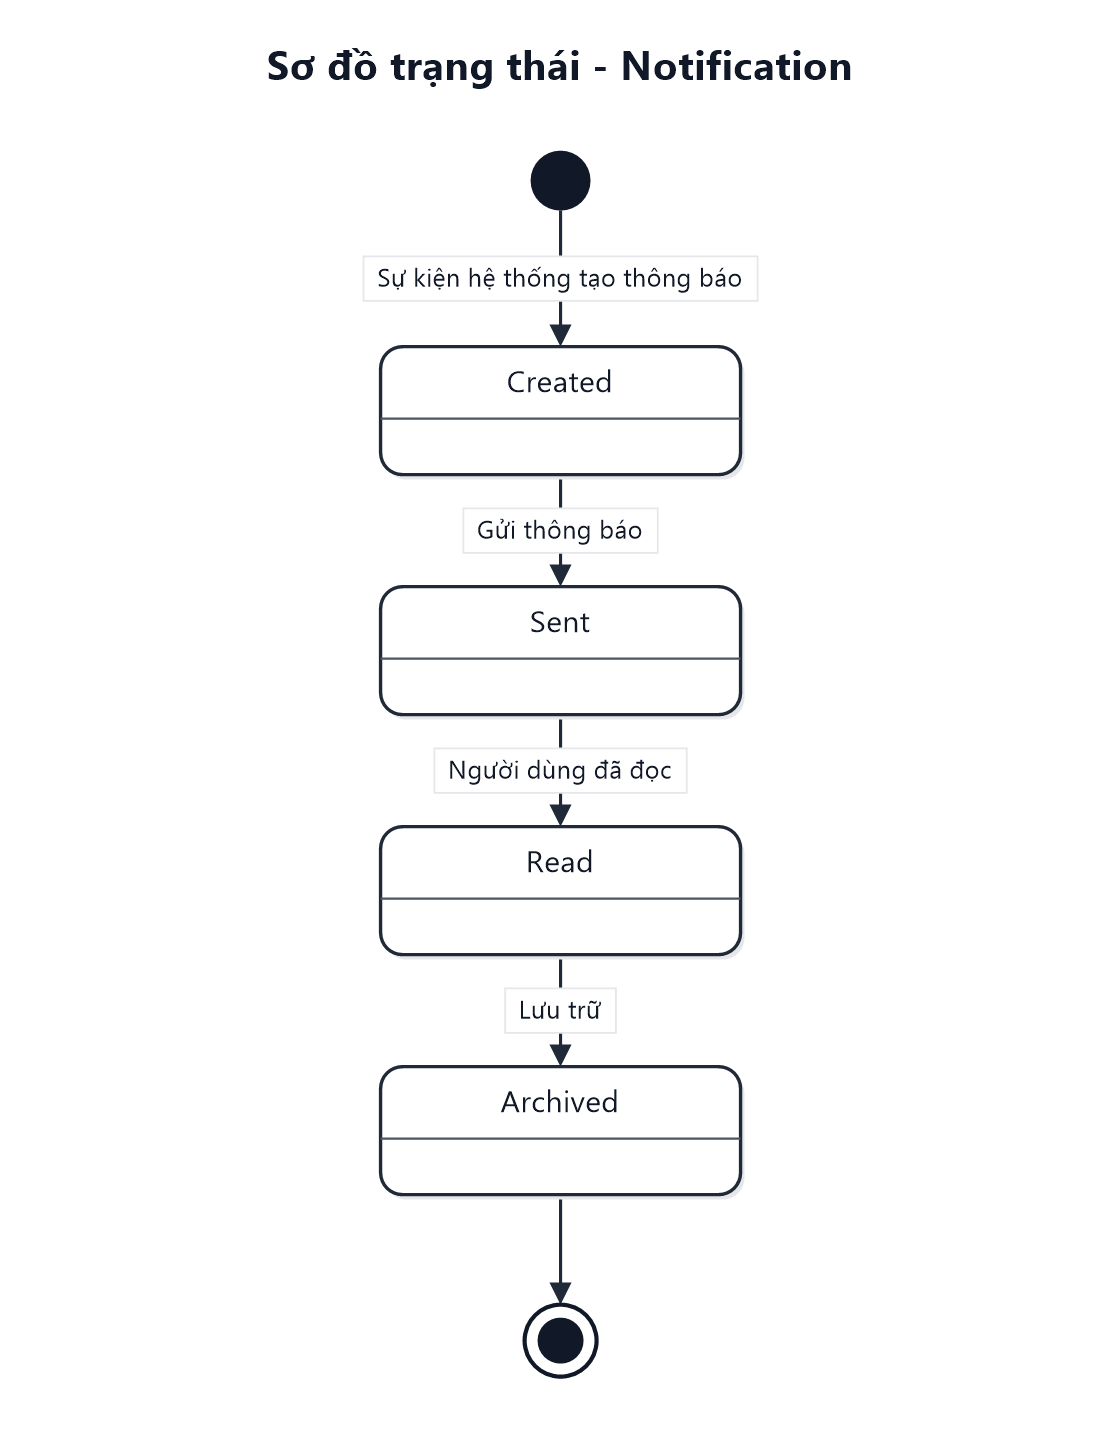
\includegraphics[width=0.82\textwidth, height=0.68\textheight, keepaspectratio]{images/state_p45_1.png}
\caption{Sơ đồ trạng thái thực thể Notification}
\end{figure}
\begin{itemize}
    \item \textbf{Các trạng thái:} \texttt{Created} (được tạo từ sự kiện) $\rightarrow$ \texttt{Sent} (đã gửi qua kênh thông báo) $\rightarrow$ \texttt{Read} (người dùng đã đọc) $\rightarrow$ \texttt{Archived} (lưu trữ tra cứu). Khi ánh xạ xuống bảng dữ liệu gọn nhẹ \texttt{Notifications}, trạng thái đã đọc/chưa đọc được lưu trực tiếp qua cờ \texttt{Is\_Read}.
\end{itemize}

\subsubsection{Sơ đồ trạng thái Membership\_Plans}
\begin{figure}[H]
\centering
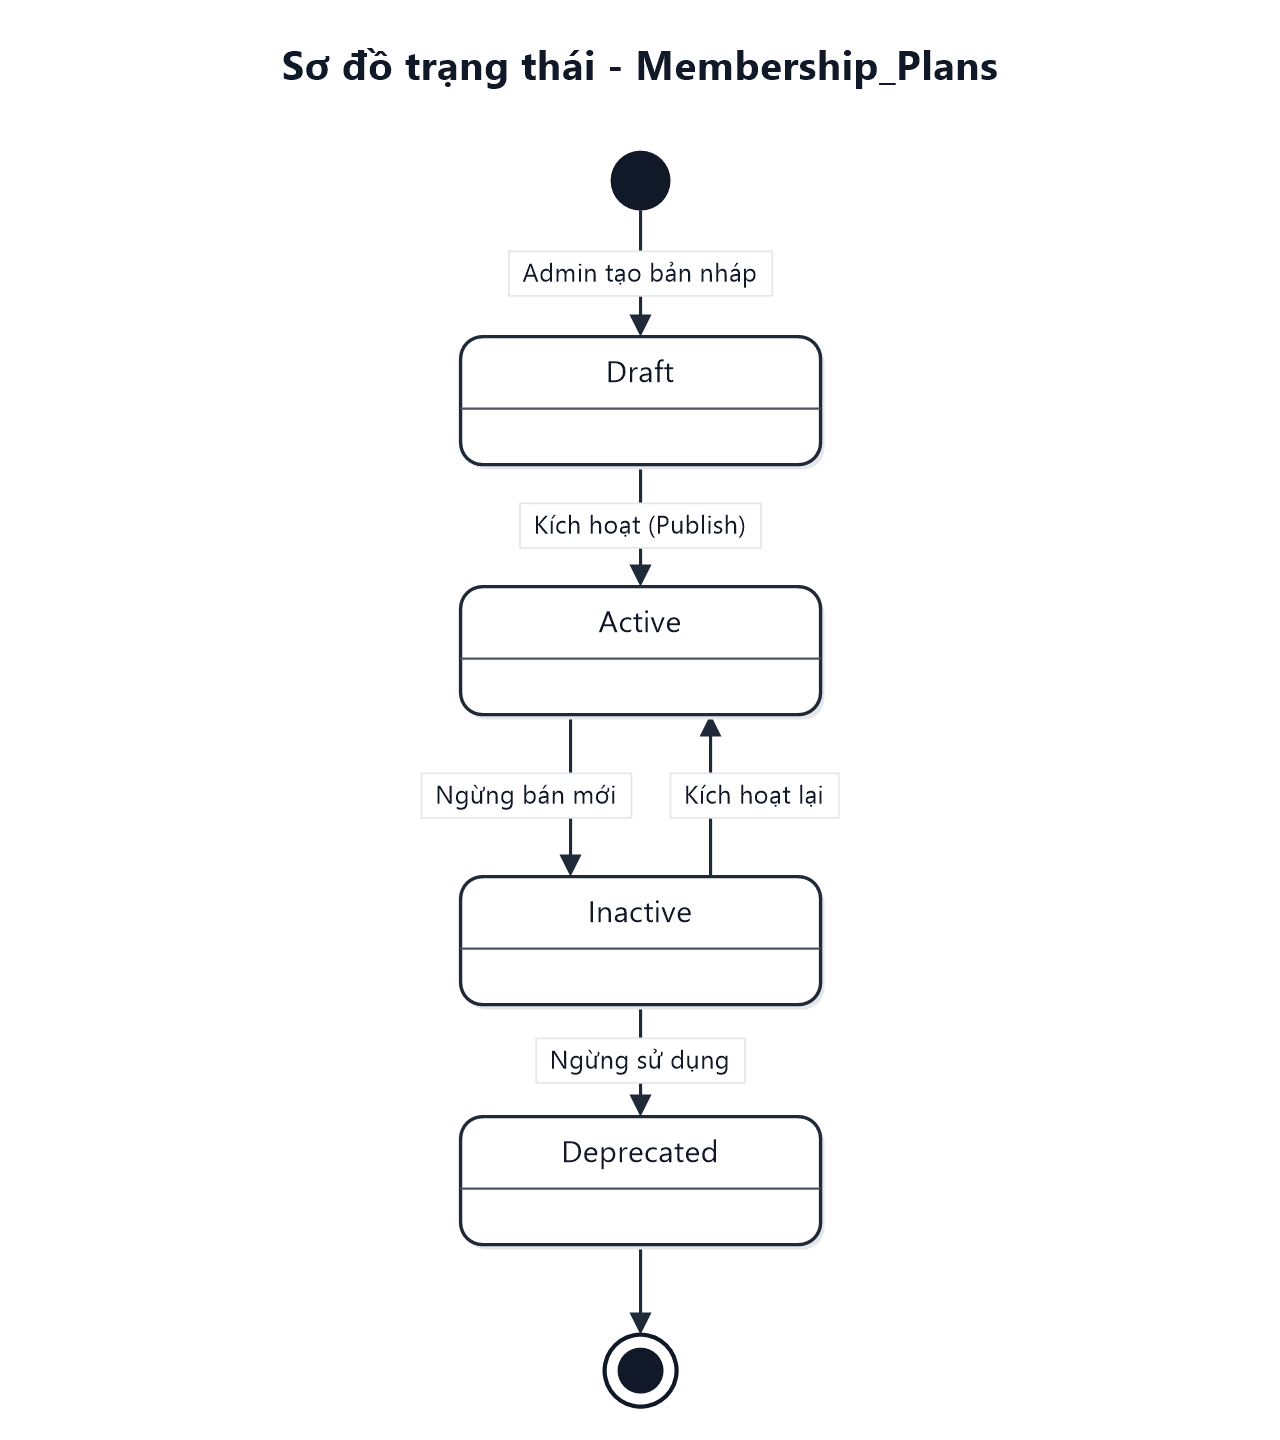
\includegraphics[width=0.82\textwidth, height=0.68\textheight, keepaspectratio]{images/state_p47_1.png}
\caption{Sơ đồ trạng thái thực thể Membership\_Plans}
\end{figure}
\begin{itemize}
    \item \textbf{Các trạng thái:} \texttt{Draft} (bản nháp) $\rightarrow$ \texttt{Active} (hiển thị cho hội viên đăng ký) $\leftrightarrow$ \texttt{Inactive} (ngừng bán mới) $\rightarrow$ \texttt{Deprecated} (ngừng sử dụng, chỉ lưu lịch sử).
\end{itemize}

\subsubsection{Sơ đồ trạng thái Equipment}
\begin{figure}[H]
\centering
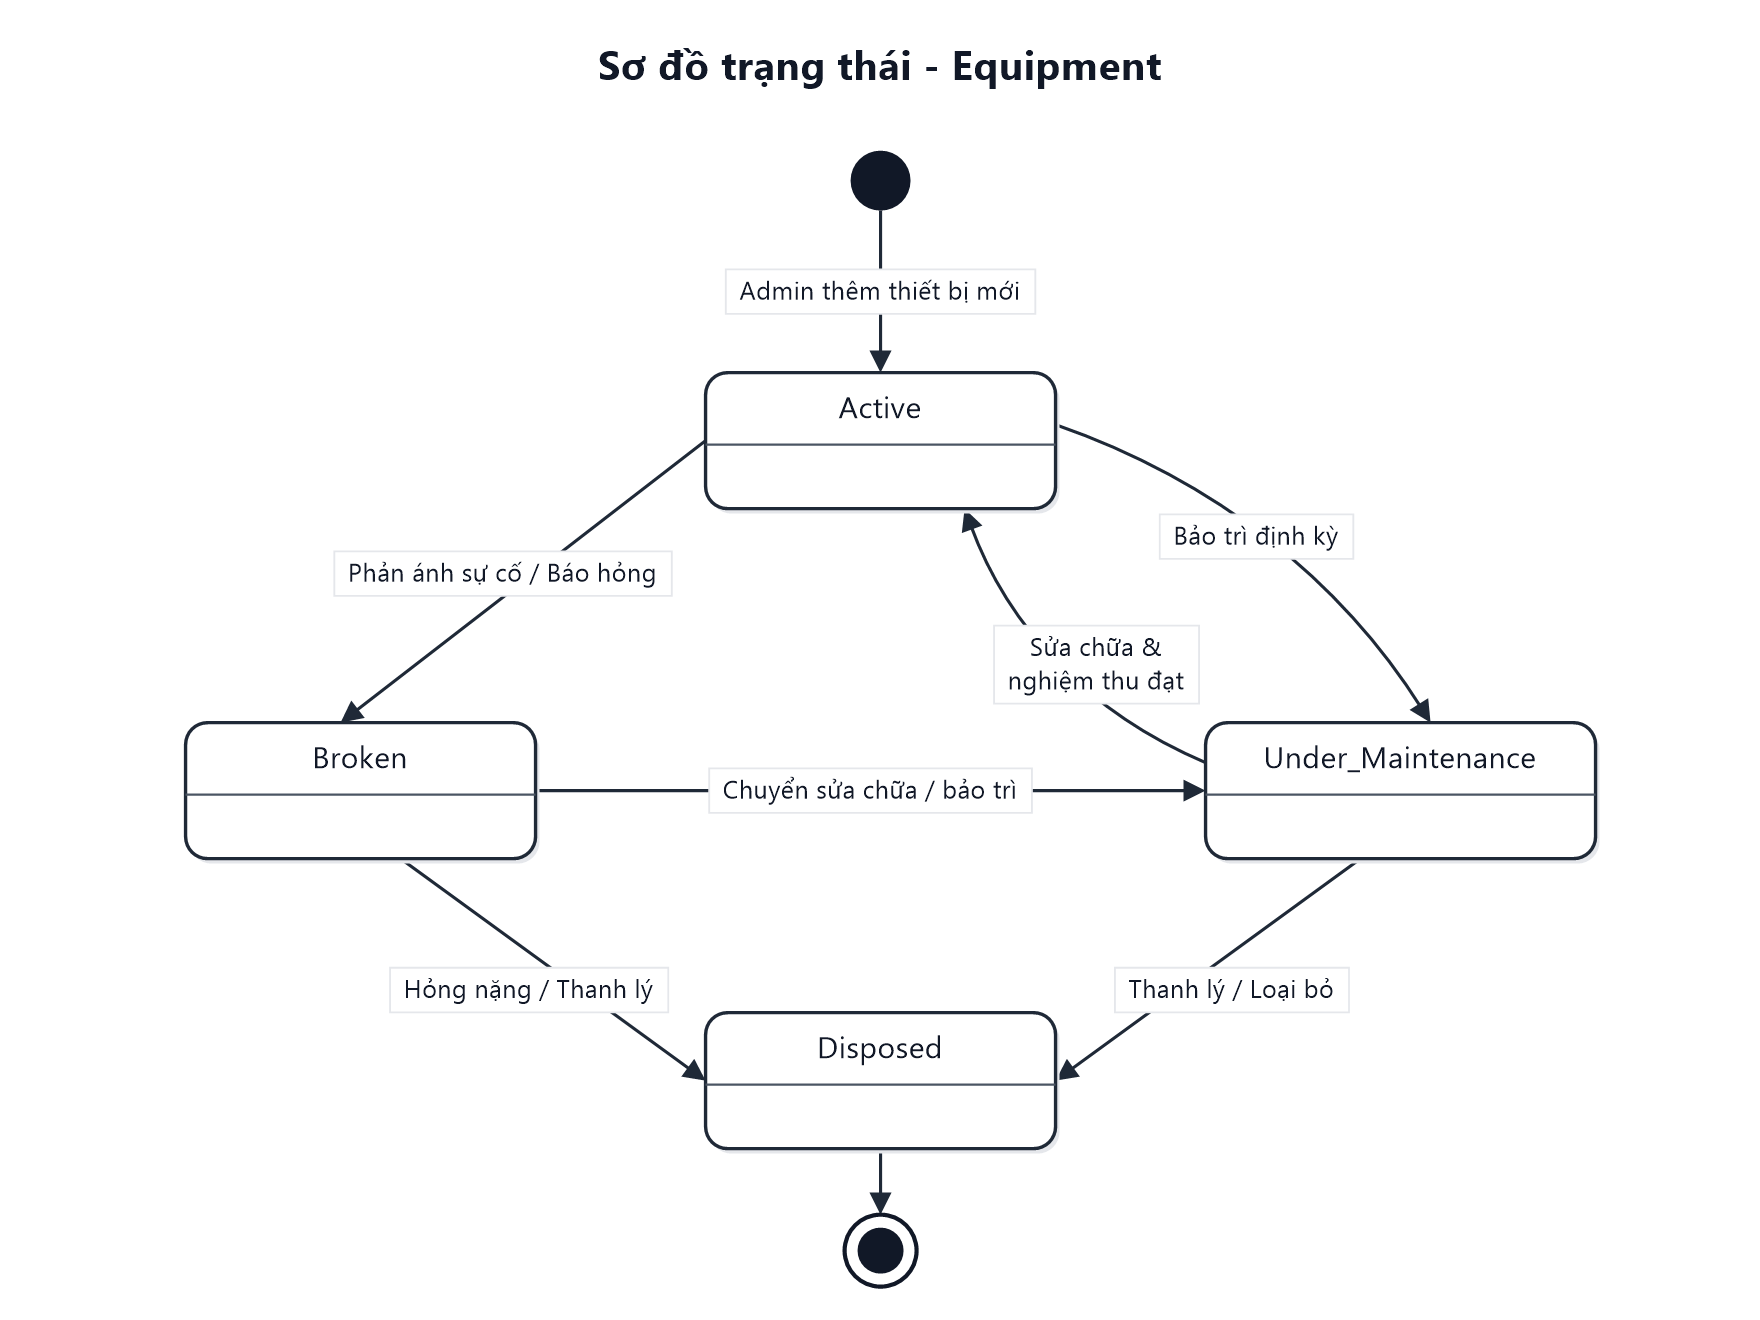
\includegraphics[width=0.82\textwidth, height=0.68\textheight, keepaspectratio]{images/state_p49_1.png}
\caption{Sơ đồ trạng thái thực thể Equipment}
\end{figure}
\begin{itemize}
    \item \textbf{Các trạng thái:} \texttt{Active} (thiết bị mới thêm, hoạt động bình thường) $\rightarrow$ \texttt{Broken} (phản ánh sự cố / báo hỏng) $\leftrightarrow$ \texttt{Under\_Maintenance} (đang bảo trì / sửa chữa; nghiệm thu đạt quay lại \texttt{Active}) $\rightarrow$ \texttt{Disposed} (hỏng nặng / thanh lý).
\end{itemize}

\subsubsection{Sơ đồ trạng thái Equipment\_Issues}
\begin{figure}[H]
\centering
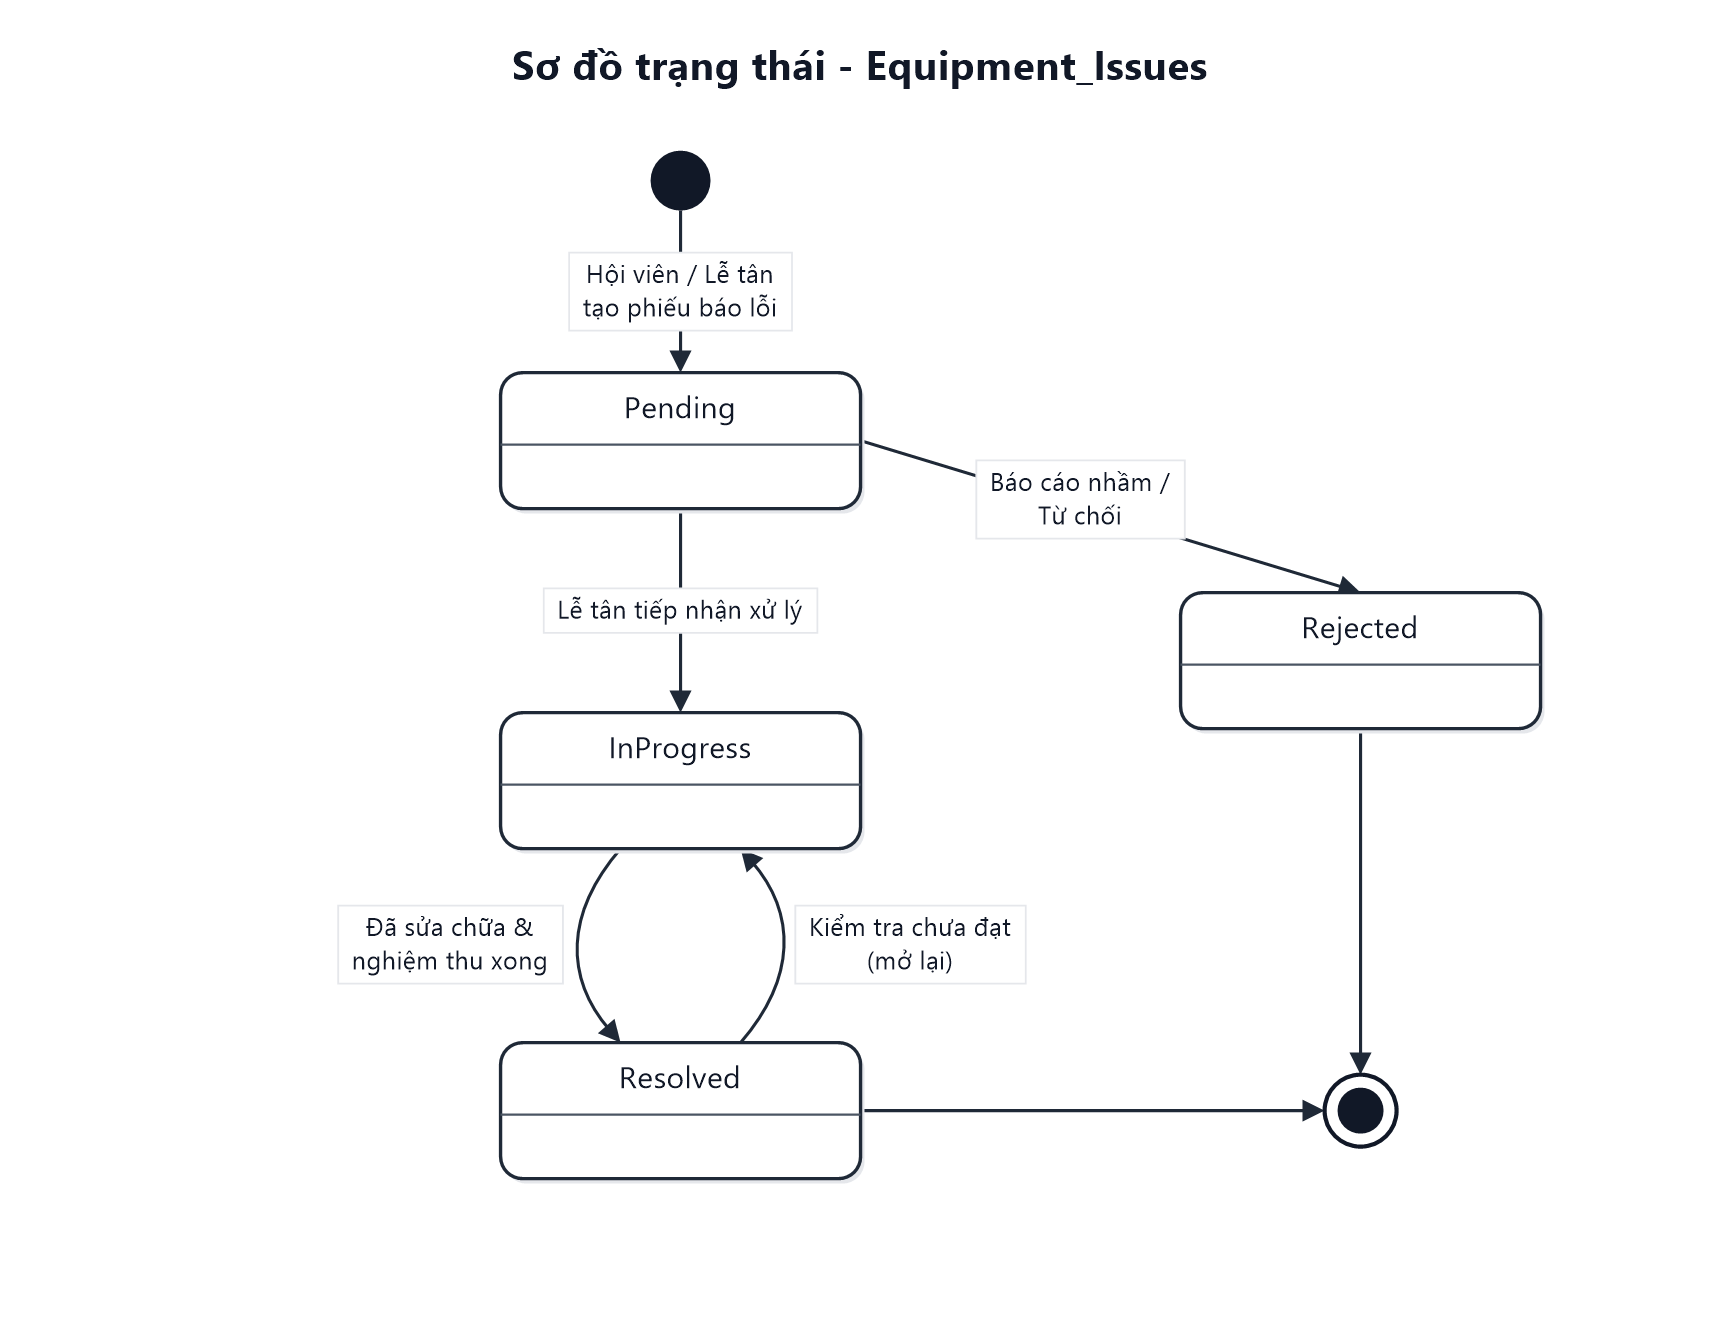
\includegraphics[width=0.82\textwidth, height=0.68\textheight, keepaspectratio]{images/state_p51_1.png}
\caption{Sơ đồ trạng thái thực thể Equipment\_Issues}
\end{figure}
\begin{itemize}
    \item \textbf{Các trạng thái:} \texttt{Pending} (phiếu báo lỗi mới do Hội viên hoặc Lễ tân tạo) $\rightarrow$ \texttt{InProgress} (Lễ tân tiếp nhận, kỹ thuật đang xử lý) $\leftrightarrow$ \texttt{Resolved} (đã sửa chữa xong và nghiệm thu; mở lại \texttt{InProgress} nếu kiểm tra chưa đạt), hoặc \texttt{Rejected} (từ chối / hủy phiếu do báo cáo nhầm).
\end{itemize}

\subsubsection{Sơ đồ trạng thái Trainer\_Availability}
\begin{figure}[H]
\centering
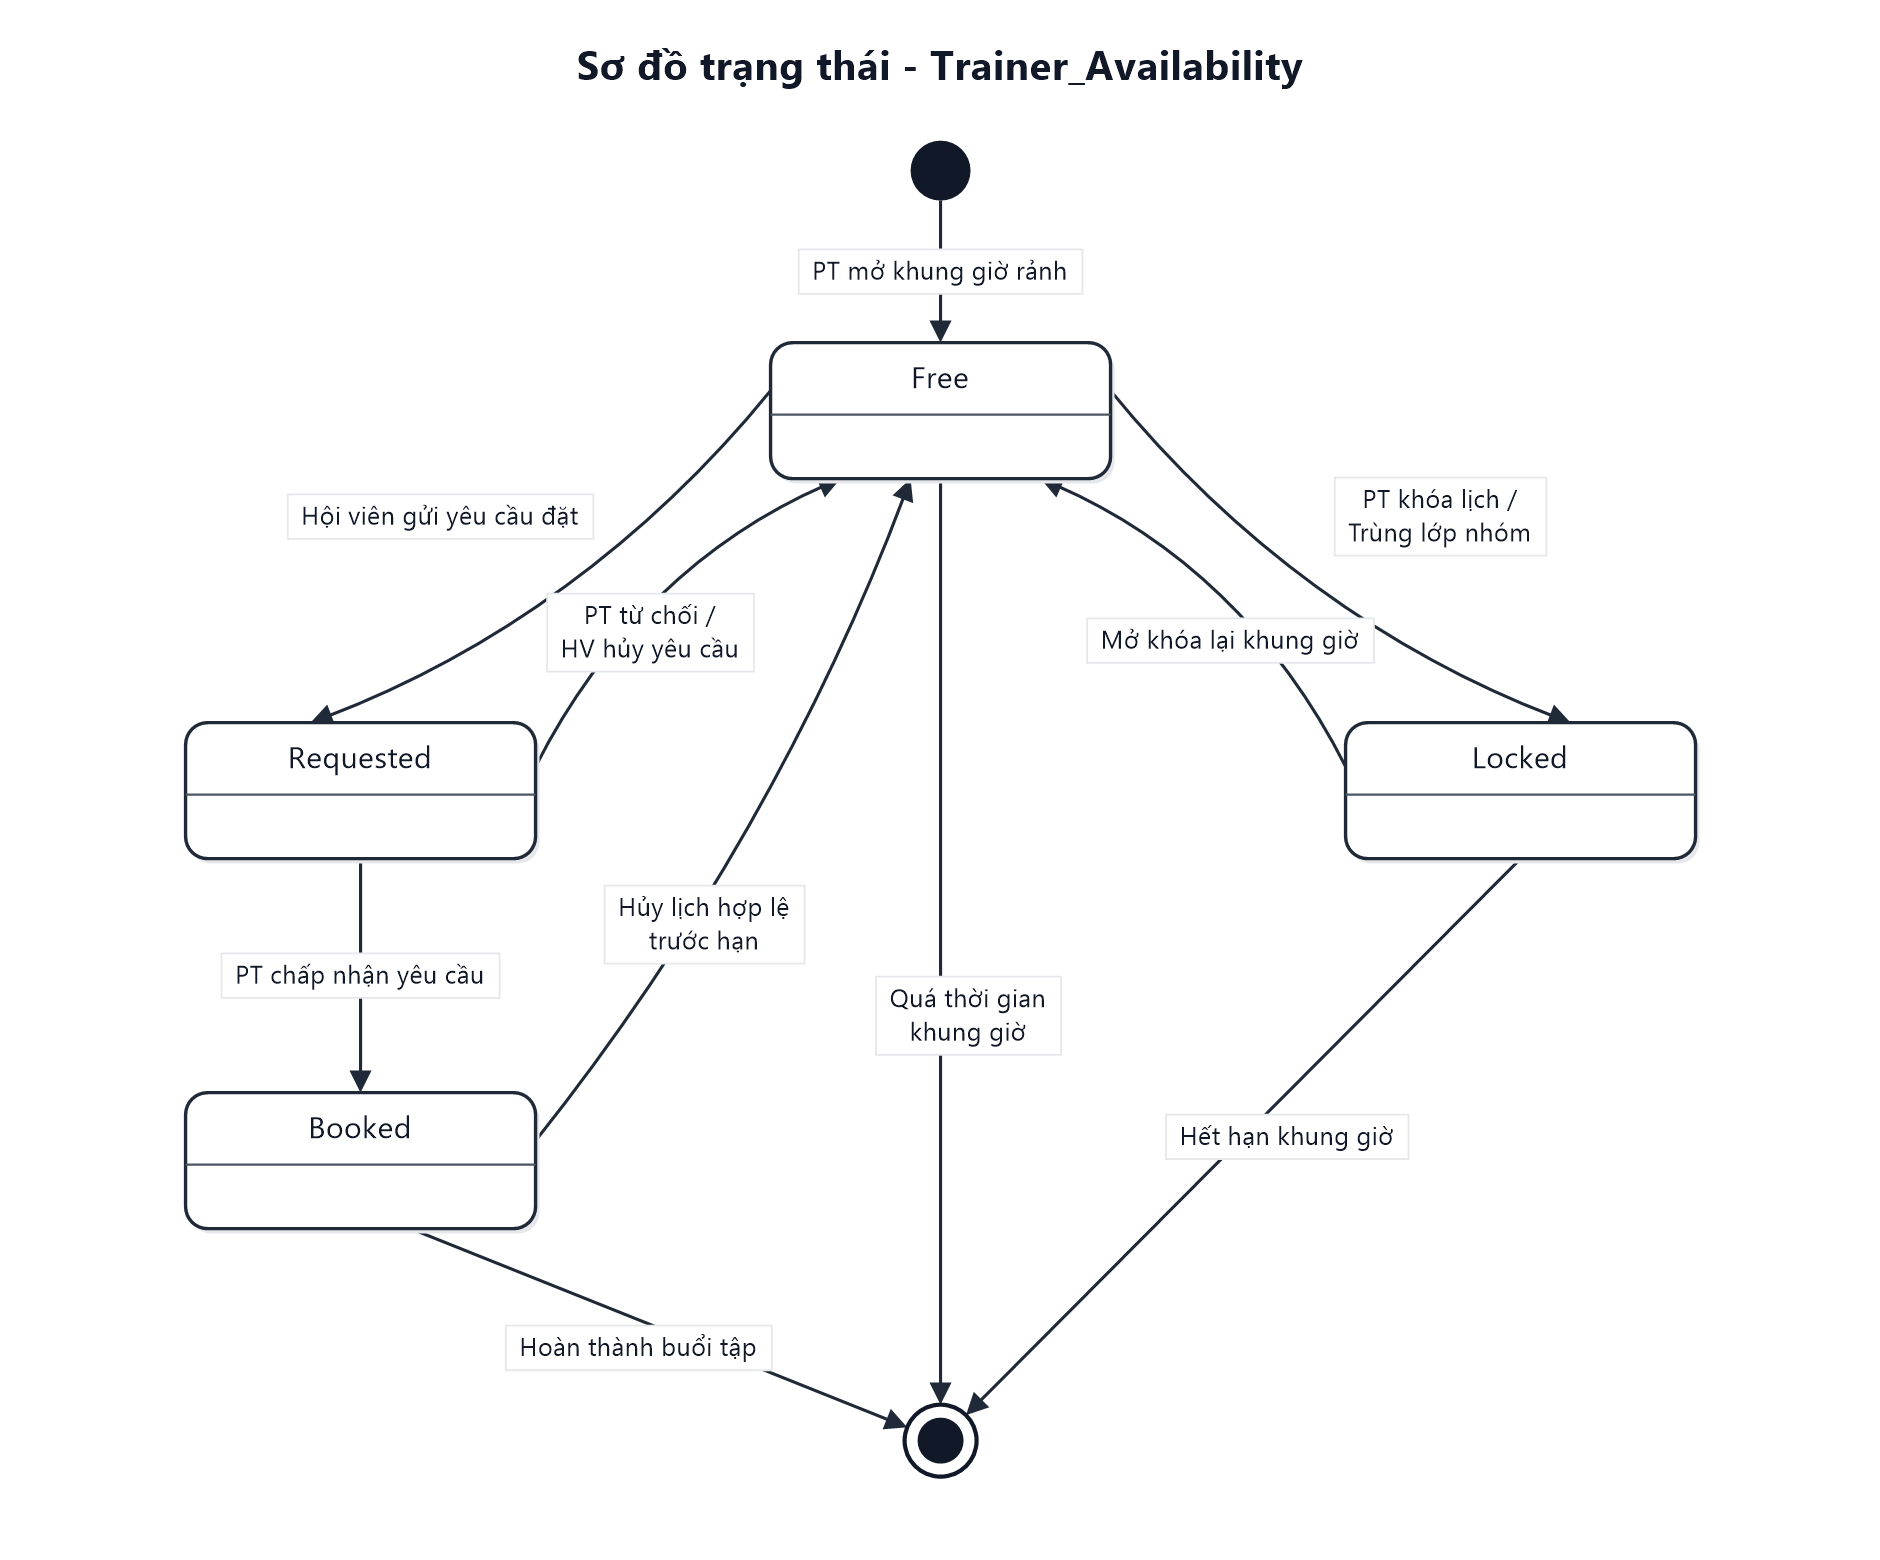
\includegraphics[width=0.82\textwidth, height=0.68\textheight, keepaspectratio]{images/state_p53_1.png}
\caption{Sơ đồ trạng thái thực thể Trainer\_Availability}
\end{figure}
\begin{itemize}
    \item \textbf{Các trạng thái:} \texttt{Free} (khung giờ rảnh mở đặt) $\leftrightarrow$ \texttt{Requested} (hội viên gửi yêu cầu đặt) $\rightarrow$ \texttt{Booked} (PT chấp nhận, có thể về \texttt{Free} nếu hủy hợp lệ trước hạn), và \texttt{Locked} (PT khóa lịch hoặc trùng lớp nhóm). Các khung giờ \texttt{Free/Locked} tự kết thúc khi quá thời gian hiệu lực; dưới mức lưu trữ \texttt{Trainer\_Availabilities}, trạng thái trống/đã đặt lưu gọn qua cờ \texttt{Is\_Booked} kết hợp đối chiếu với \texttt{Bookings} và \texttt{Class\_Sessions}.
\end{itemize}

\subsubsection{Sơ đồ trạng thái Trainer}
\begin{figure}[H]
\centering
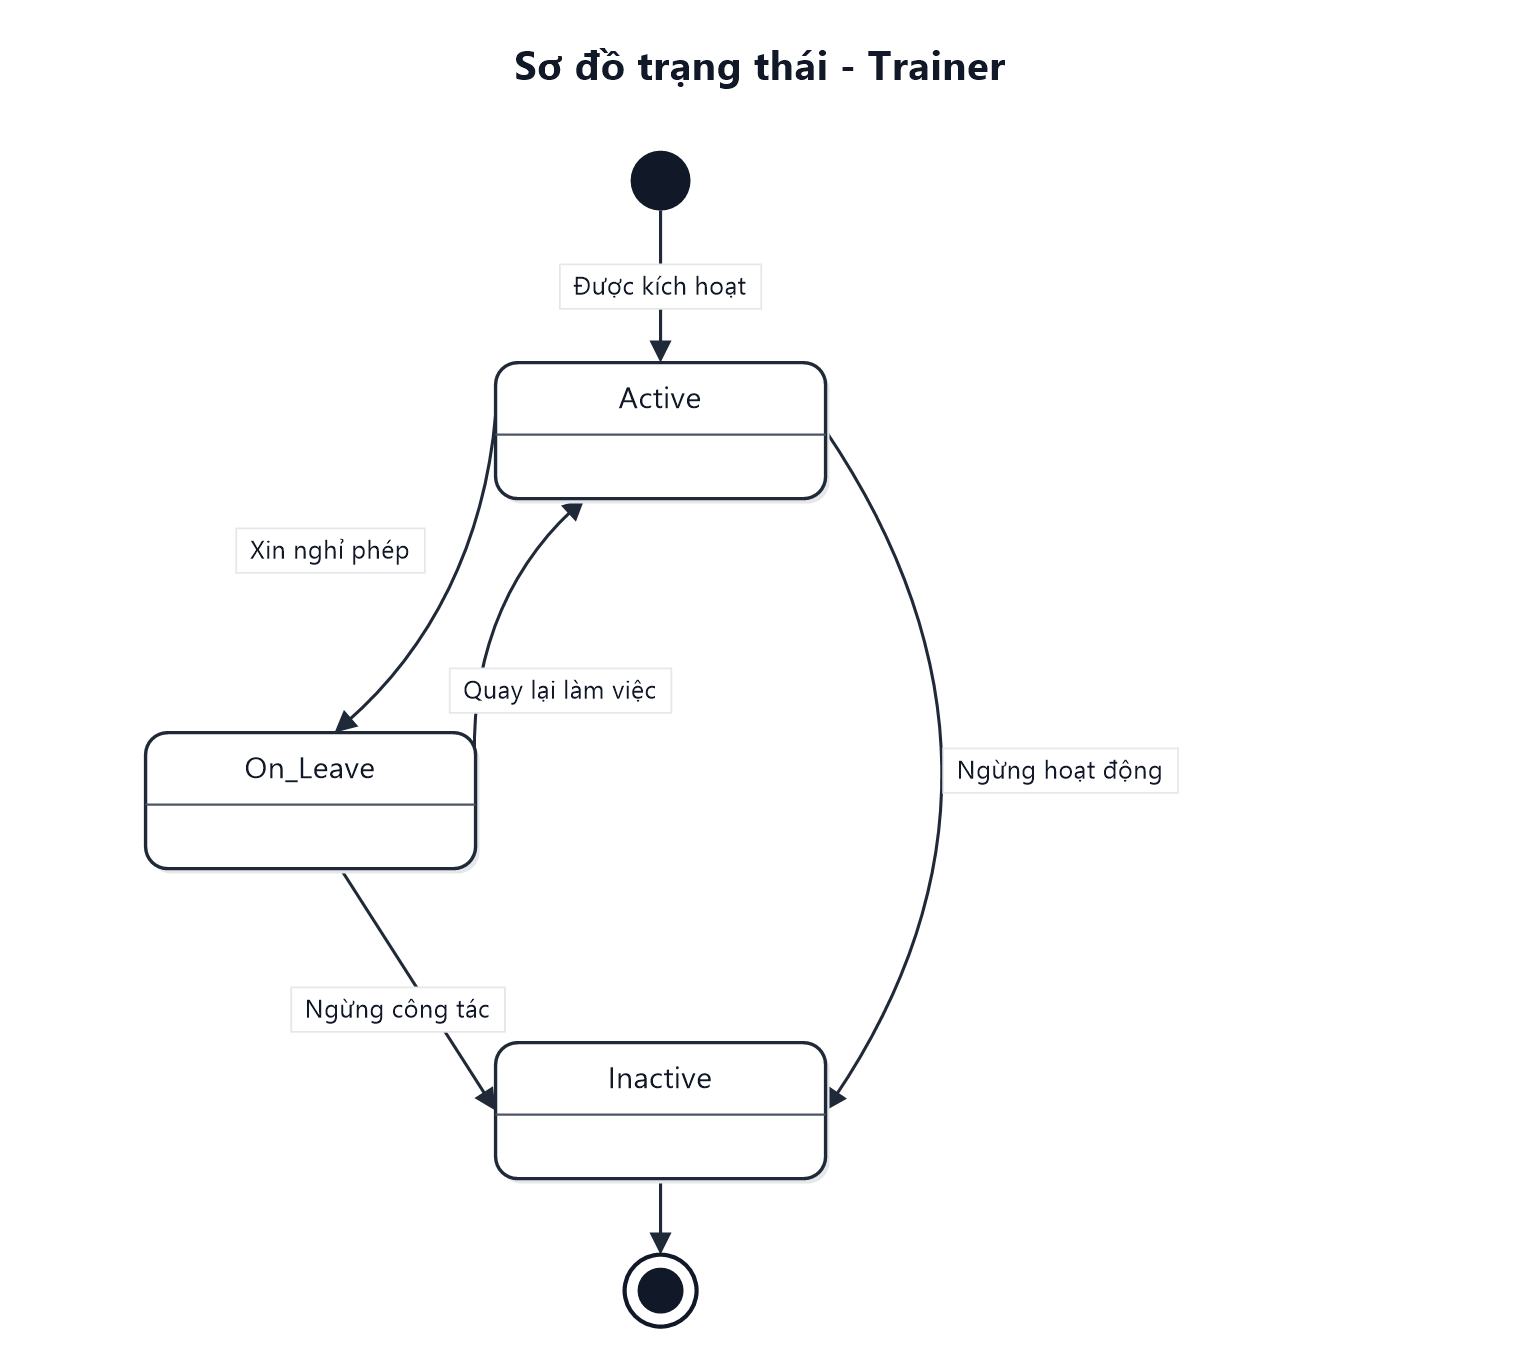
\includegraphics[width=0.82\textwidth, height=0.68\textheight, keepaspectratio]{images/state_p55_1.png}
\caption{Sơ đồ trạng thái thực thể Trainer}
\end{figure}
\begin{itemize}
    \item \textbf{Các trạng thái:} \texttt{Active} (đang giảng dạy) $\leftrightarrow$ \texttt{On\_Leave} (đang nghỉ phép, tạm ngừng nhận lịch mới) $\rightarrow$ \texttt{Inactive} (ngừng công tác).
\end{itemize}

\subsubsection{Sơ đồ trạng thái Staff}
\begin{figure}[H]
\centering
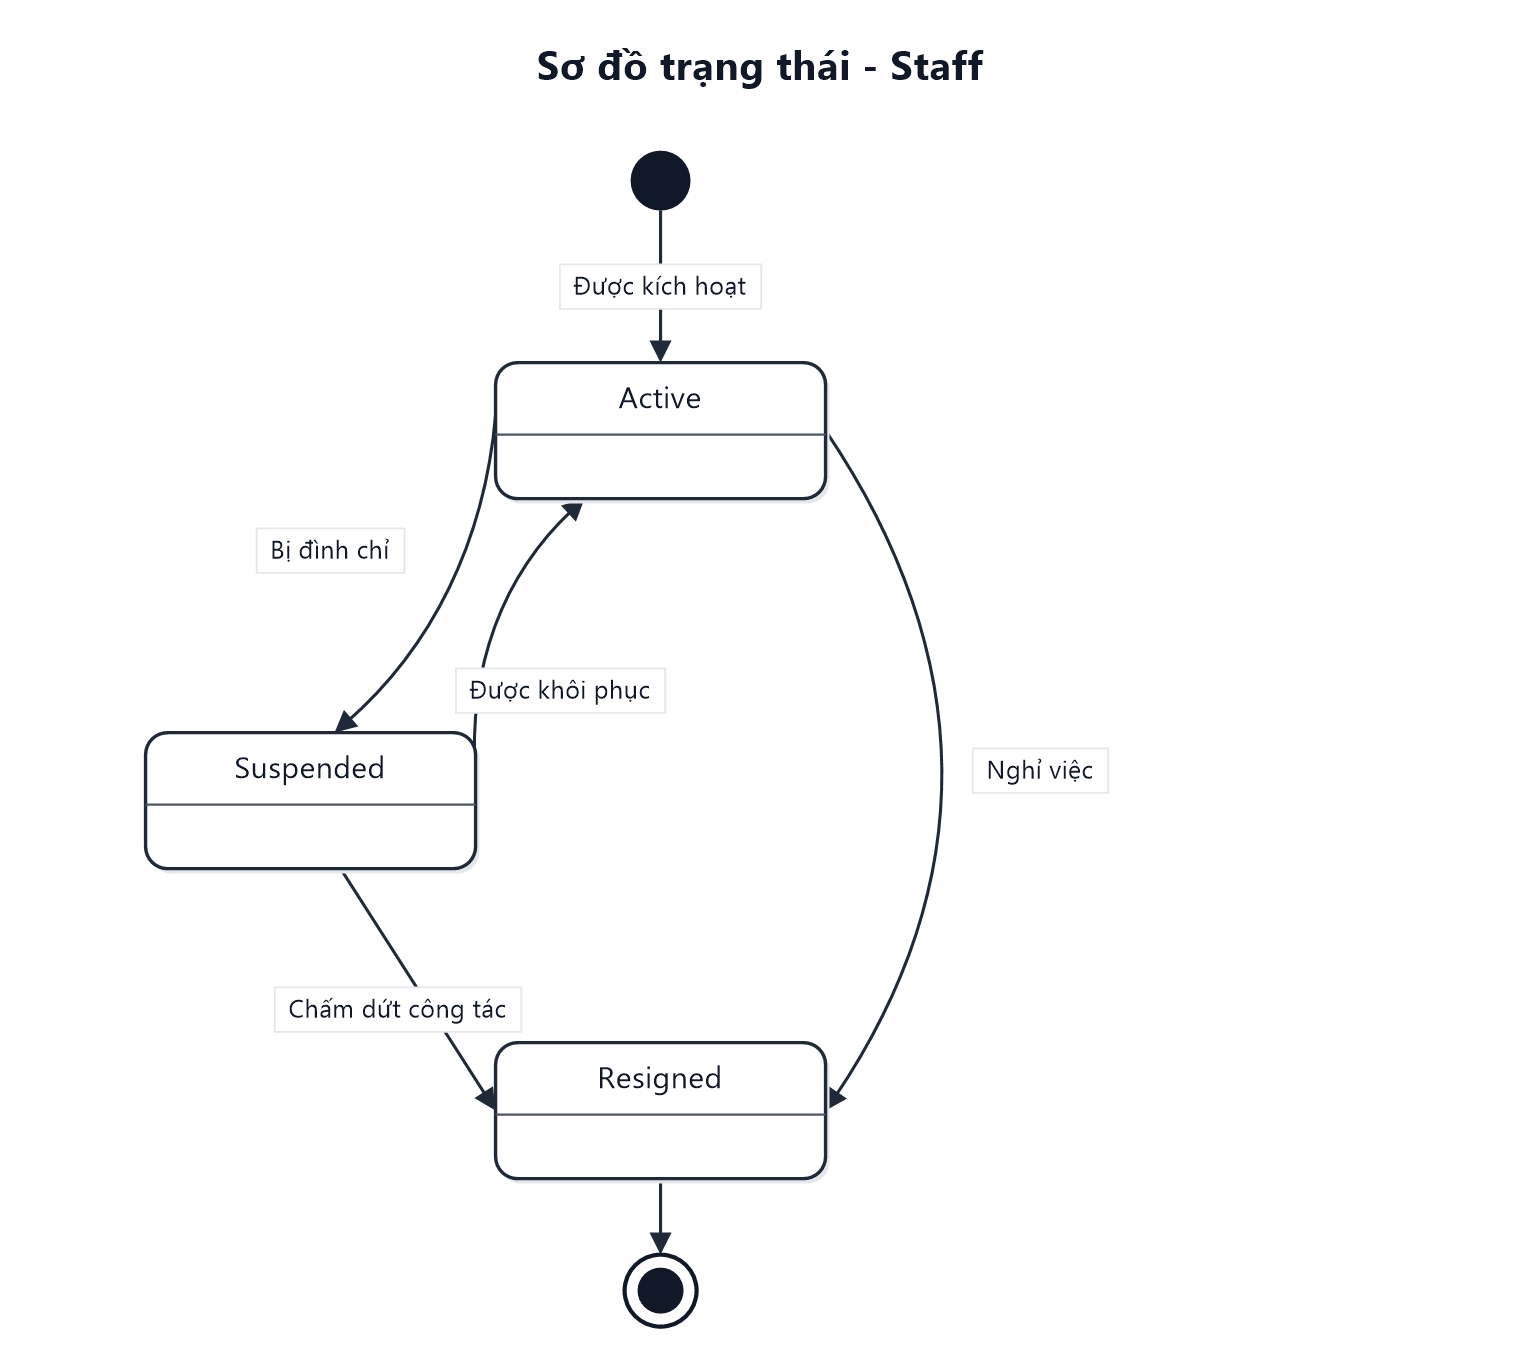
\includegraphics[width=0.82\textwidth, height=0.68\textheight, keepaspectratio]{images/state_p57_1.png}
\caption{Sơ đồ trạng thái thực thể Staff}
\end{figure}
\begin{itemize}
    \item \textbf{Các trạng thái:} \texttt{Active} (đang làm việc theo chi nhánh) $\leftrightarrow$ \texttt{Suspended} (tạm đình chỉ) $\rightarrow$ \texttt{Resigned} (nghỉ việc, thu hồi quyền truy cập).
\end{itemize}

\subsubsection{Sơ đồ trạng thái Branches}
\begin{figure}[H]
\centering
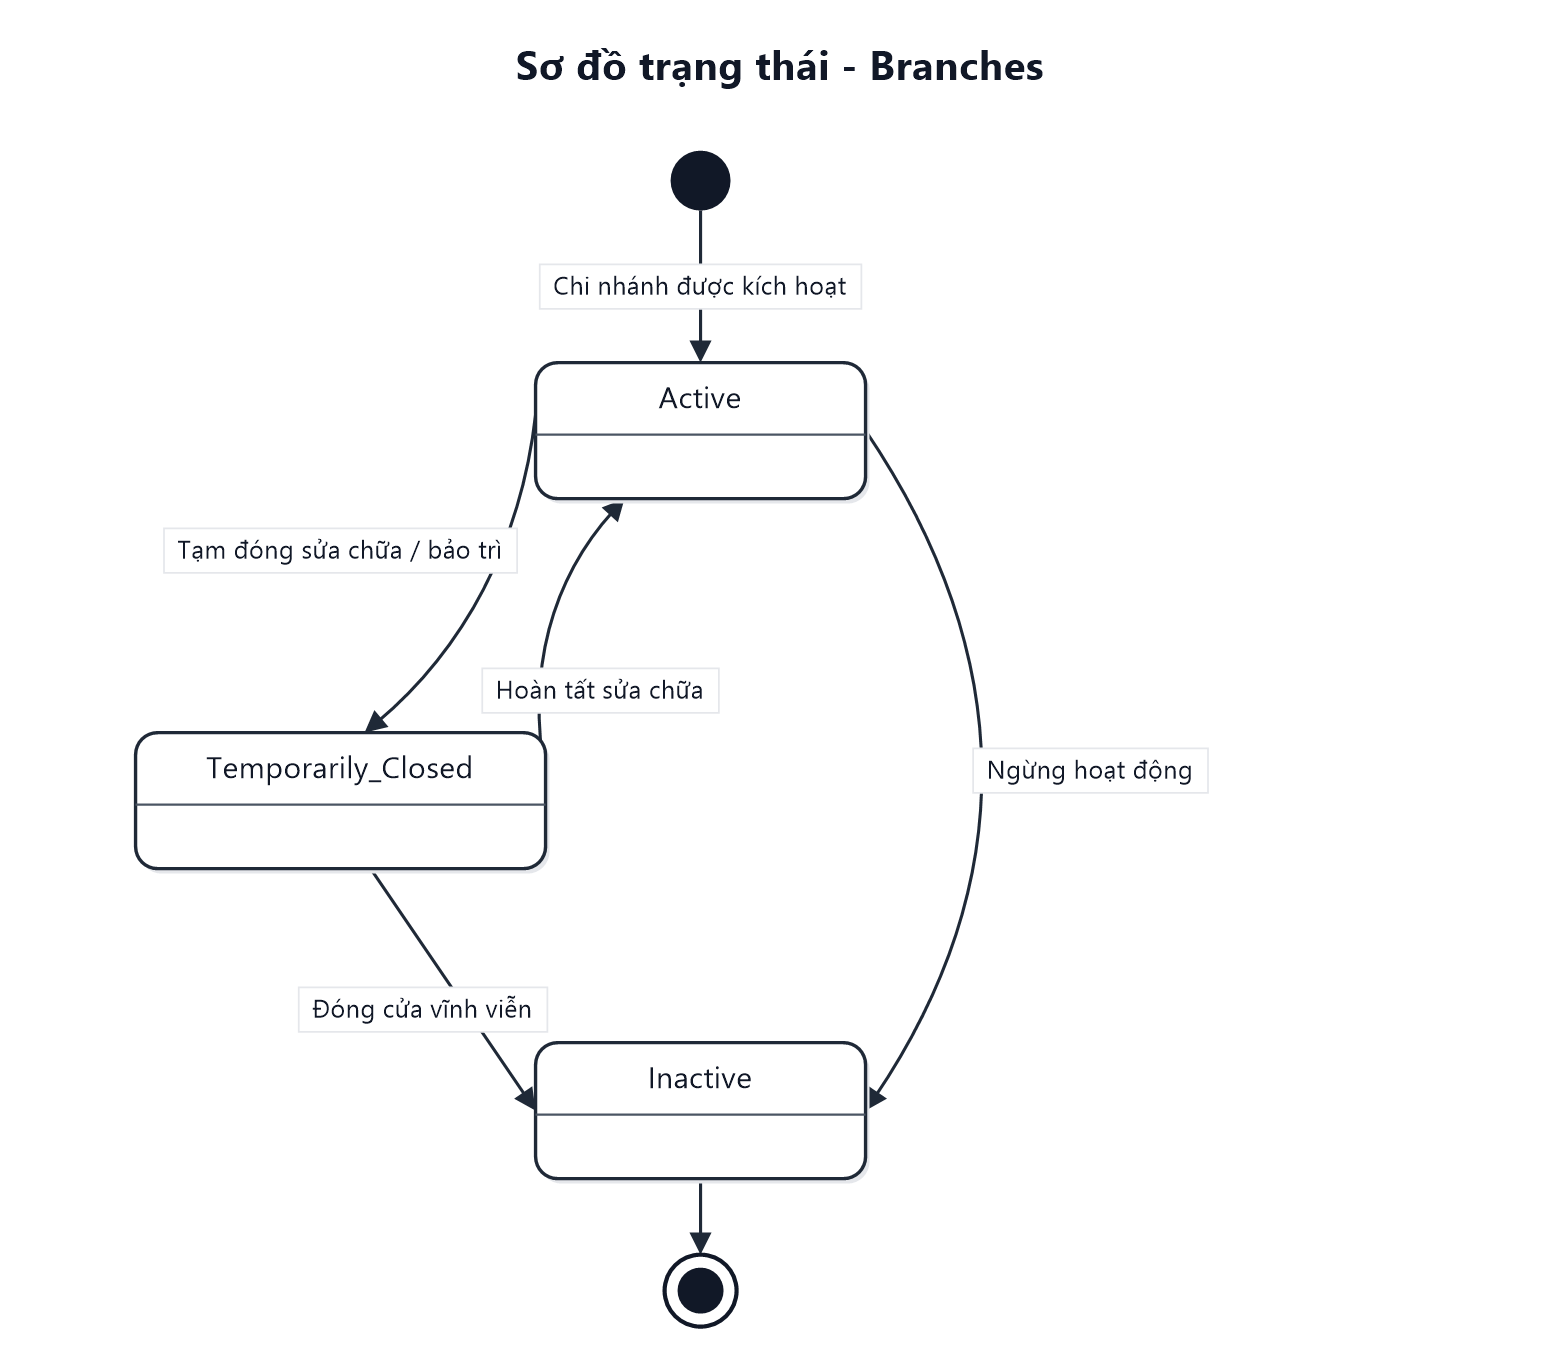
\includegraphics[width=0.82\textwidth, height=0.68\textheight, keepaspectratio]{images/state_p59_1.png}
\caption{Sơ đồ trạng thái thực thể Branches}
\end{figure}
\begin{itemize}
    \item \textbf{Các trạng thái:} \texttt{Active} (hoạt động bình thường) $\leftrightarrow$ \texttt{Temporarily\_Closed} (tạm đóng cửa sửa chữa/bảo trì) $\rightarrow$ \texttt{Inactive} (đóng cửa vĩnh viễn, xử lý các lớp tồn đọng và lưu lịch sử).
\end{itemize}

% ==============================================================================
% 4. THIẾT KẾ DỮ LIỆU
% ==============================================================================
\newpage
\section{Thiết kế dữ liệu}

\subsection{Sơ đồ logic cơ sở dữ liệu}
Sơ đồ logic (Logical Database Schema) dưới đây thể hiện toàn bộ \textbf{23 bảng dữ liệu} cùng khóa chính (PK), khóa ngoại (FK) và mối quan hệ liên kết trong hệ thống \textbf{DFGymCenter}.

\begin{figure}[H]
\centering
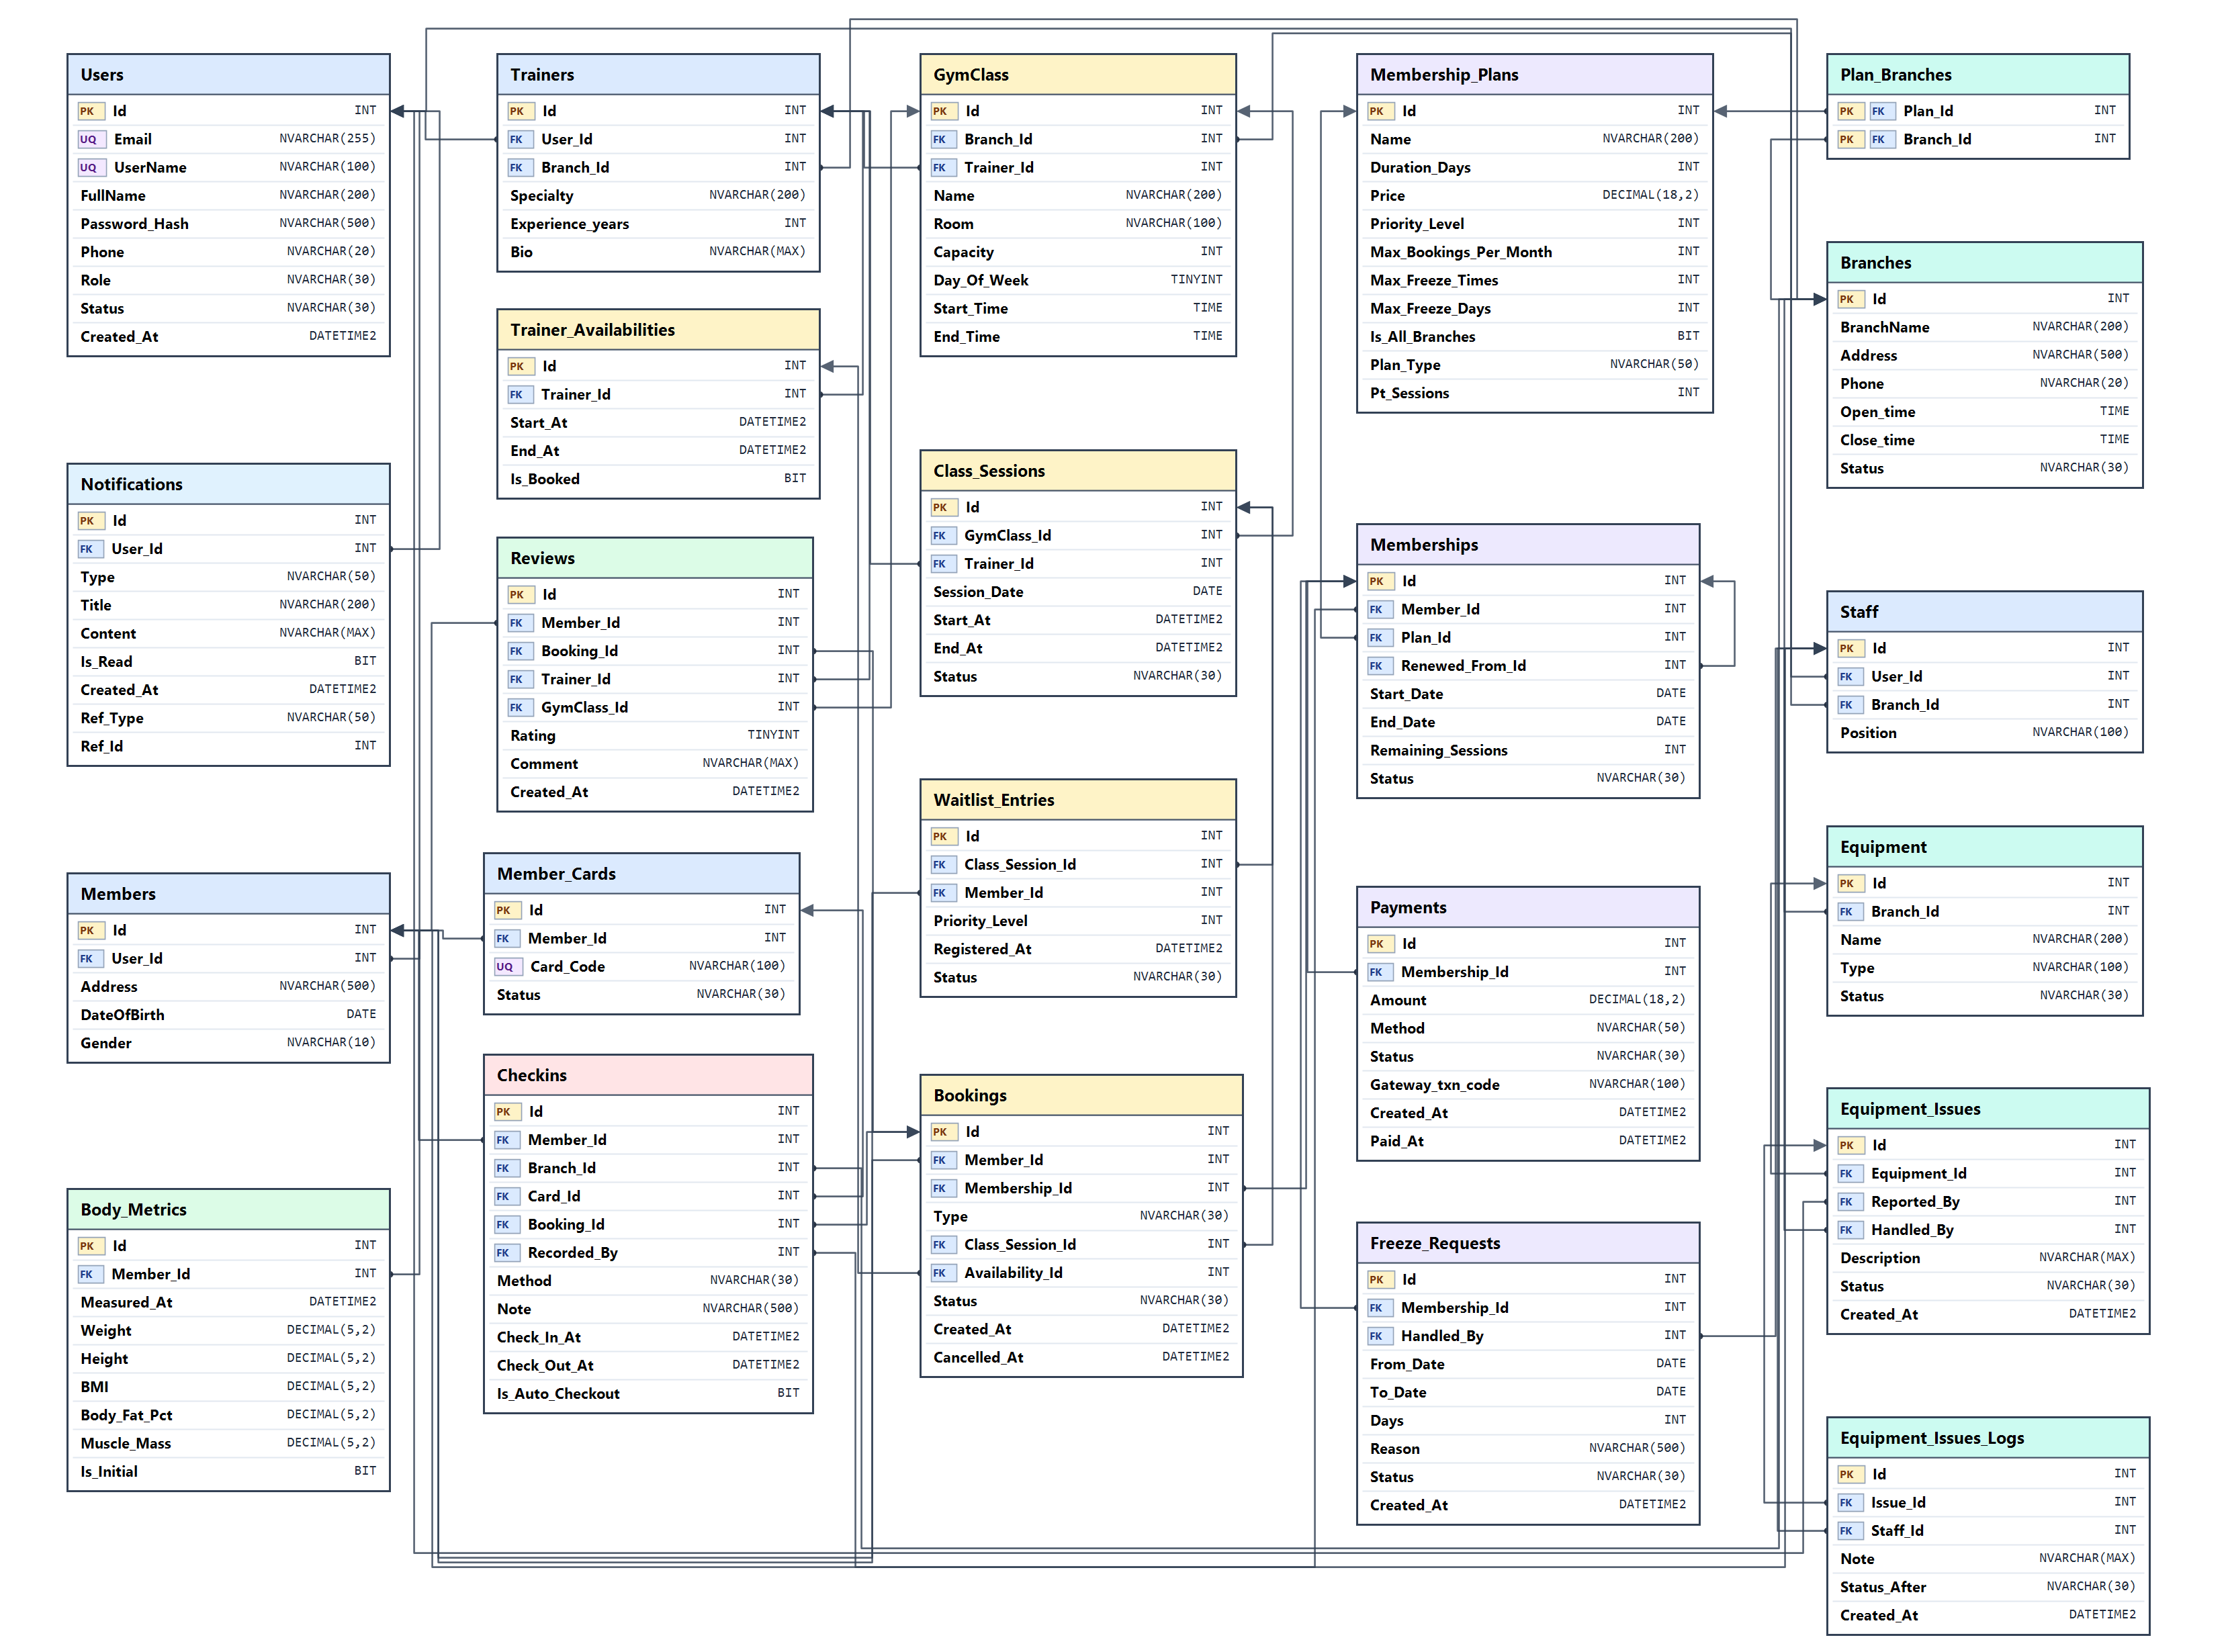
\includegraphics[width=\textwidth, height=0.80\textheight, keepaspectratio]{images/csdl_p03_1.png}
\caption{Sơ đồ logic cơ sở dữ liệu hệ thống DFGymCenter}
\end{figure}

\subsection{Mô tả chi tiết các bảng dữ liệu}
Dưới đây là đặc tả chi tiết 23 bảng dữ liệu trong sơ đồ logic (kiểu dữ liệu, ràng buộc và ý nghĩa):

\subsubsection{Users -- Người dùng hệ thống}
\begin{figure}[H]
\centering
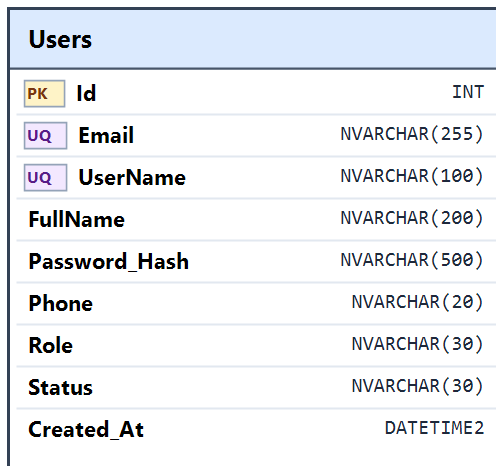
\includegraphics[width=0.34\textwidth]{images/tbl_Users.png}
\end{figure}
\begin{table}[H]\centering\footnotesize
\begin{tabularx}{\textwidth}{|c|L{3.0cm}|L{2.8cm}|L{3.2cm}|Y|}
\hline \textbf{STT} & \textbf{Tên thuộc tính} & \textbf{Kiểu} & \textbf{Ràng buộc} & \textbf{Ý nghĩa / Ghi chú} \\ \hline
1 & \texttt{Id} & \texttt{INT} & PK, NN, tự tăng & Mã người dùng \\ \hline
2 & \texttt{Email} & \texttt{NVARCHAR(255)} & NN, UQ & Email đăng nhập/liên hệ \\ \hline
3 & \texttt{UserName} & \texttt{NVARCHAR(100)} & NN, UQ & Tên đăng nhập \\ \hline
4 & \texttt{FullName} & \texttt{NVARCHAR(200)} & NN & Họ và tên \\ \hline
5 & \texttt{Password\_Hash} & \texttt{NVARCHAR(500)} & NN & Mật khẩu đã băm \\ \hline
6 & \texttt{Phone} & \texttt{NVARCHAR(20)} & & Số điện thoại \\ \hline
7 & \texttt{Role} & \texttt{NVARCHAR(30)} & NN & Vai trò: Admin / Staff / Trainer / Member \\ \hline
8 & \texttt{Status} & \texttt{NVARCHAR(30)} & NN, DF \texttt{'Active'} & Trạng thái tài khoản \\ \hline
9 & \texttt{Created\_At} & \texttt{DATETIME2} & NN, DF hiện tại & Thời điểm tạo tài khoản \\ \hline
\end{tabularx}
\end{table}

\subsubsection{Branches -- Chi nhánh}
\begin{figure}[H]
\centering
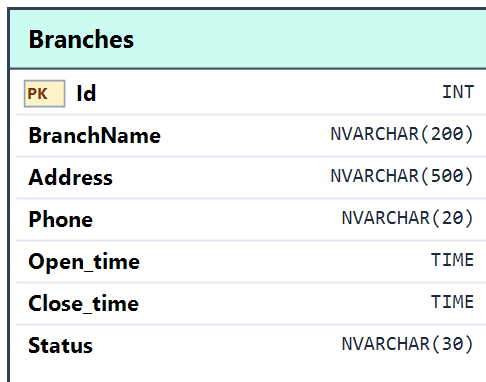
\includegraphics[width=0.34\textwidth]{images/tbl_Branches.png}
\end{figure}
\begin{table}[H]\centering\footnotesize
\begin{tabularx}{\textwidth}{|c|L{3.0cm}|L{2.8cm}|L{3.2cm}|Y|}
\hline \textbf{STT} & \textbf{Tên thuộc tính} & \textbf{Kiểu} & \textbf{Ràng buộc} & \textbf{Ý nghĩa / Ghi chú} \\ \hline
1 & \texttt{Id} & \texttt{INT} & PK, NN, tự tăng & Mã chi nhánh \\ \hline
2 & \texttt{BranchName} & \texttt{NVARCHAR(200)} & NN & Tên chi nhánh \\ \hline
3 & \texttt{Address} & \texttt{NVARCHAR(500)} & & Địa chỉ \\ \hline
4 & \texttt{Phone} & \texttt{NVARCHAR(20)} & & Số điện thoại chi nhánh \\ \hline
5 & \texttt{Open\_time} & \texttt{TIME} & & Giờ mở cửa \\ \hline
6 & \texttt{Close\_time} & \texttt{TIME} & & Giờ đóng cửa \\ \hline
7 & \texttt{Status} & \texttt{NVARCHAR(30)} & NN, DF \texttt{'Active'} & Trạng thái hoạt động \\ \hline
\end{tabularx}
\end{table}

\subsubsection{Staff -- Nhân viên}
\begin{figure}[H]
\centering
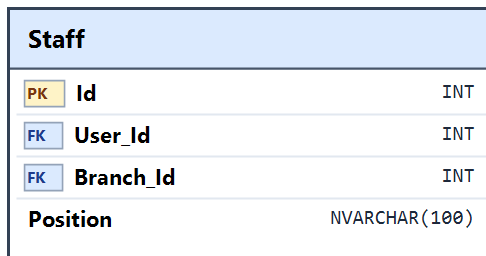
\includegraphics[width=0.34\textwidth]{images/tbl_Staff.png}
\end{figure}
\begin{table}[H]\centering\footnotesize
\begin{tabularx}{\textwidth}{|c|L{3.0cm}|L{2.8cm}|L{3.8cm}|Y|}
\hline \textbf{STT} & \textbf{Tên thuộc tính} & \textbf{Kiểu} & \textbf{Ràng buộc} & \textbf{Ý nghĩa / Ghi chú} \\ \hline
1 & \texttt{Id} & \texttt{INT} & PK, NN, tự tăng & Mã nhân viên \\ \hline
2 & \texttt{User\_Id} & \texttt{INT} & FK $\rightarrow$ \texttt{Users(Id)}, NN, UQ & Tài khoản nhân viên (1--0..1) \\ \hline
3 & \texttt{Branch\_Id} & \texttt{INT} & FK $\rightarrow$ \texttt{Branches(Id)}, NN & Chi nhánh làm việc \\ \hline
4 & \texttt{Position} & \texttt{NVARCHAR(100)} & & Chức vụ \\ \hline
\end{tabularx}
\end{table}

\subsubsection{Trainers -- Huấn luyện viên}
\begin{figure}[H]
\centering
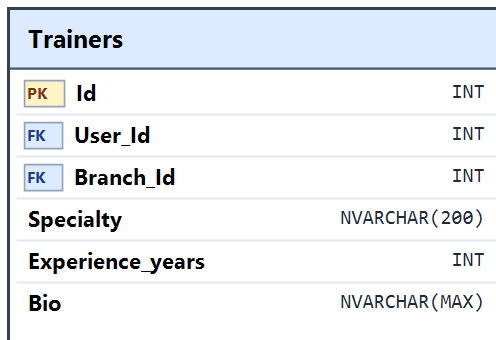
\includegraphics[width=0.34\textwidth]{images/tbl_Trainers.png}
\end{figure}
\begin{table}[H]\centering\footnotesize
\begin{tabularx}{\textwidth}{|c|L{3.0cm}|L{2.8cm}|L{3.8cm}|Y|}
\hline \textbf{STT} & \textbf{Tên thuộc tính} & \textbf{Kiểu} & \textbf{Ràng buộc} & \textbf{Ý nghĩa / Ghi chú} \\ \hline
1 & \texttt{Id} & \texttt{INT} & PK, NN, tự tăng & Mã huấn luyện viên \\ \hline
2 & \texttt{User\_Id} & \texttt{INT} & FK $\rightarrow$ \texttt{Users(Id)}, NN, UQ & Tài khoản HLV (1--0..1) \\ \hline
3 & \texttt{Branch\_Id} & \texttt{INT} & FK $\rightarrow$ \texttt{Branches(Id)}, NN & Chi nhánh trực thuộc \\ \hline
4 & \texttt{Specialty} & \texttt{NVARCHAR(200)} & & Chuyên môn \\ \hline
5 & \texttt{Experience\_years} & \texttt{INT} & CHECK $\ge 0$ & Số năm kinh nghiệm \\ \hline
6 & \texttt{Bio} & \texttt{NVARCHAR(MAX)} & & Giới thiệu bản thân \\ \hline
\end{tabularx}
\end{table}

\subsubsection{Members -- Hội viên}
\begin{figure}[H]
\centering
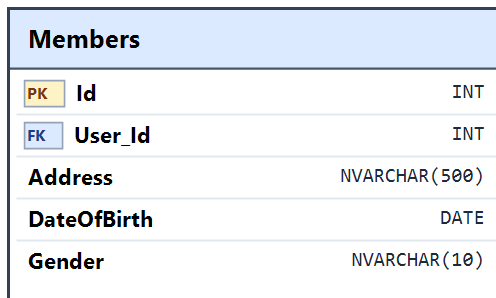
\includegraphics[width=0.34\textwidth]{images/tbl_Members.png}
\end{figure}
\begin{table}[H]\centering\footnotesize
\begin{tabularx}{\textwidth}{|c|L{3.0cm}|L{2.8cm}|L{3.8cm}|Y|}
\hline \textbf{STT} & \textbf{Tên thuộc tính} & \textbf{Kiểu} & \textbf{Ràng buộc} & \textbf{Ý nghĩa / Ghi chú} \\ \hline
1 & \texttt{Id} & \texttt{INT} & PK, NN, tự tăng & Mã hội viên \\ \hline
2 & \texttt{User\_Id} & \texttt{INT} & FK $\rightarrow$ \texttt{Users(Id)}, NN, UQ & Tài khoản hội viên (1--0..1) \\ \hline
3 & \texttt{Address} & \texttt{NVARCHAR(500)} & & Địa chỉ \\ \hline
4 & \texttt{DateOfBirth} & \texttt{DATE} & & Ngày sinh \\ \hline
5 & \texttt{Gender} & \texttt{NVARCHAR(10)} & & Giới tính \\ \hline
\end{tabularx}
\end{table}

\subsubsection{Member\_Cards -- Thẻ hội viên}
\begin{figure}[H]
\centering
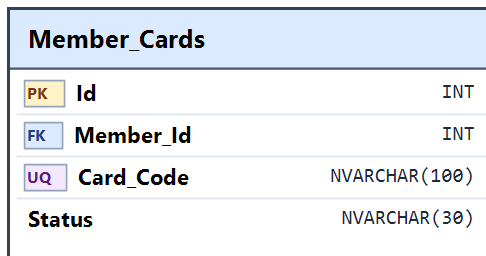
\includegraphics[width=0.34\textwidth]{images/tbl_Member_Cards.png}
\end{figure}
\begin{table}[H]\centering\footnotesize
\begin{tabularx}{\textwidth}{|c|L{3.0cm}|L{2.8cm}|L{3.8cm}|Y|}
\hline \textbf{STT} & \textbf{Tên thuộc tính} & \textbf{Kiểu} & \textbf{Ràng buộc} & \textbf{Ý nghĩa / Ghi chú} \\ \hline
1 & \texttt{Id} & \texttt{INT} & PK, NN, tự tăng & Mã thẻ \\ \hline
2 & \texttt{Member\_Id} & \texttt{INT} & FK $\rightarrow$ \texttt{Members(Id)}, NN & Hội viên sở hữu thẻ \\ \hline
3 & \texttt{Card\_Code} & \texttt{NVARCHAR(100)} & NN, UQ & Mã thẻ (QR/RFID) dùng khi check-in \\ \hline
4 & \texttt{Status} & \texttt{NVARCHAR(30)} & NN, DF \texttt{'Active'} & Trạng thái thẻ (\texttt{Active}, \texttt{Locked}, \texttt{Lost}, \texttt{Replaced}; riêng \texttt{Lost} vô hiệu vĩnh viễn không mở khóa lại) \\ \hline
\end{tabularx}
\end{table}

\subsubsection{Body\_Metrics -- Chỉ số cơ thể}
\begin{figure}[H]
\centering
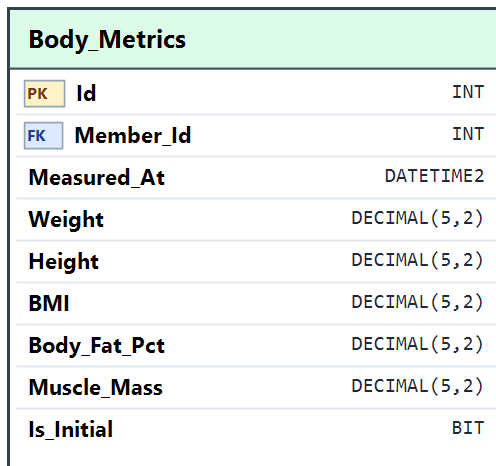
\includegraphics[width=0.34\textwidth]{images/tbl_Body_Metrics.png}
\end{figure}
\begin{table}[H]\centering\footnotesize
\begin{tabularx}{\textwidth}{|c|L{3.0cm}|L{2.8cm}|L{3.8cm}|Y|}
\hline \textbf{STT} & \textbf{Tên thuộc tính} & \textbf{Kiểu} & \textbf{Ràng buộc} & \textbf{Ý nghĩa / Ghi chú} \\ \hline
1 & \texttt{Id} & \texttt{INT} & PK, NN, tự tăng & Mã bản ghi chỉ số \\ \hline
2 & \texttt{Member\_Id} & \texttt{INT} & FK $\rightarrow$ \texttt{Members(Id)}, NN & Hội viên được đo \\ \hline
3 & \texttt{Measured\_At} & \texttt{DATETIME2} & NN, DF hiện tại & Thời điểm đo \\ \hline
4 & \texttt{Weight} & \texttt{DECIMAL(5,2)} & & Cân nặng (kg) \\ \hline
5 & \texttt{Height} & \texttt{DECIMAL(5,2)} & & Chiều cao (cm) \\ \hline
6 & \texttt{BMI} & \texttt{DECIMAL(5,2)} & & Chỉ số khối cơ thể \\ \hline
7 & \texttt{Body\_Fat\_Pct} & \texttt{DECIMAL(5,2)} & & Tỷ lệ mỡ cơ thể (\%) \\ \hline
8 & \texttt{Muscle\_Mass} & \texttt{DECIMAL(5,2)} & & Khối lượng cơ (kg) \\ \hline
9 & \texttt{Is\_Initial} & \texttt{BIT} & NN, DF \texttt{0} & Đánh dấu lần đo ban đầu (1 = lần đầu) \\ \hline
\end{tabularx}
\end{table}

\subsubsection{Equipment -- Thiết bị}
\begin{figure}[H]
\centering
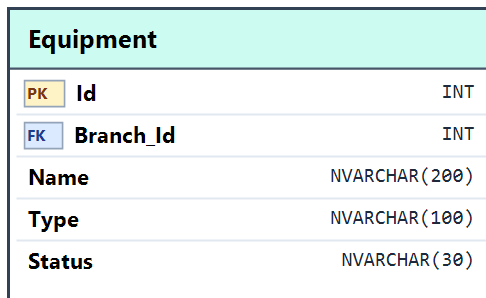
\includegraphics[width=0.34\textwidth]{images/tbl_Equipment.png}
\end{figure}
\begin{table}[H]\centering\footnotesize
\begin{tabularx}{\textwidth}{|c|L{3.0cm}|L{2.8cm}|L{3.8cm}|Y|}
\hline \textbf{STT} & \textbf{Tên thuộc tính} & \textbf{Kiểu} & \textbf{Ràng buộc} & \textbf{Ý nghĩa / Ghi chú} \\ \hline
1 & \texttt{Id} & \texttt{INT} & PK, NN, tự tăng & Mã thiết bị \\ \hline
2 & \texttt{Branch\_Id} & \texttt{INT} & FK $\rightarrow$ \texttt{Branches(Id)}, NN & Chi nhánh đặt thiết bị \\ \hline
3 & \texttt{Name} & \texttt{NVARCHAR(200)} & NN & Tên thiết bị \\ \hline
4 & \texttt{Type} & \texttt{NVARCHAR(100)} & & Loại thiết bị \\ \hline
5 & \texttt{Status} & \texttt{NVARCHAR(30)} & NN, DF \texttt{'Active'} & Trạng thái (\texttt{Active}, \texttt{Broken}, \texttt{Under\_\hspace{0pt}Maintenance}, \texttt{Disposed}) \\ \hline
\end{tabularx}
\end{table}

\subsubsection{Equipment\_Issues -- Sự cố thiết bị}
\begin{figure}[H]
\centering
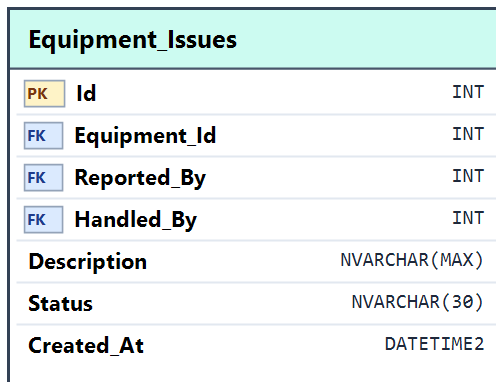
\includegraphics[width=0.34\textwidth]{images/tbl_Equipment_Issues.png}
\end{figure}
\begin{table}[H]\centering\footnotesize
\begin{tabularx}{\textwidth}{|c|L{3.0cm}|L{2.8cm}|L{3.8cm}|Y|}
\hline \textbf{STT} & \textbf{Tên thuộc tính} & \textbf{Kiểu} & \textbf{Ràng buộc} & \textbf{Ý nghĩa / Ghi chú} \\ \hline
1 & \texttt{Id} & \texttt{INT} & PK, NN, tự tăng & Mã sự cố \\ \hline
2 & \texttt{Equipment\_Id} & \texttt{INT} & FK $\rightarrow$ \texttt{Equipment(Id)}, NN & Thiết bị gặp sự cố \\ \hline
3 & \texttt{Reported\_By} & \texttt{INT} & FK $\rightarrow$ \texttt{Users(Id)}, NN & Người báo cáo sự cố \\ \hline
4 & \texttt{Handled\_By} & \texttt{INT} & FK $\rightarrow$ \texttt{Staff(Id)} & Nhân viên xử lý (NULL nếu chưa nhận) \\ \hline
5 & \texttt{Description} & \texttt{NVARCHAR(MAX)} & & Mô tả sự cố \\ \hline
6 & \texttt{Status} & \texttt{NVARCHAR(30)} & NN, DF \texttt{'Pending'} & Trạng thái xử lý (\texttt{Pending}, \texttt{InProgress}, \texttt{Resolved}, \texttt{Rejected}) \\ \hline
7 & \texttt{Created\_At} & \texttt{DATETIME2} & NN, DF hiện tại & Thời điểm báo cáo \\ \hline
\end{tabularx}
\end{table}

\subsubsection{Equipment\_Issues\_Logs -- Nhật ký xử lý sự cố}
\begin{figure}[H]
\centering
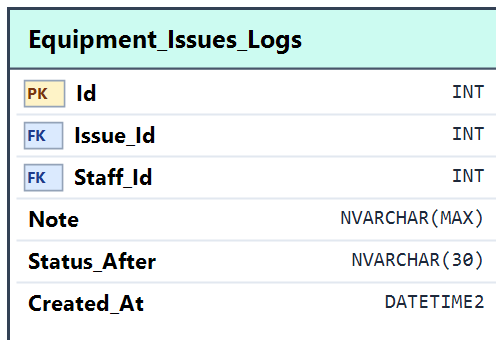
\includegraphics[width=0.34\textwidth]{images/tbl_Equipment_Issues_Logs.png}
\end{figure}
\begin{table}[H]\centering\footnotesize
\begin{tabularx}{\textwidth}{|c|L{3.0cm}|L{2.8cm}|L{4.2cm}|Y|}
\hline \textbf{STT} & \textbf{Tên thuộc tính} & \textbf{Kiểu} & \textbf{Ràng buộc} & \textbf{Ý nghĩa / Ghi chú} \\ \hline
1 & \texttt{Id} & \texttt{INT} & PK, NN, tự tăng & Mã nhật ký \\ \hline
2 & \texttt{Issue\_Id} & \texttt{INT} & FK $\rightarrow$ \texttt{Equipment\_Issues(Id)}, NN & Sự cố liên quan \\ \hline
3 & \texttt{Staff\_Id} & \texttt{INT} & FK $\rightarrow$ \texttt{Staff(Id)}, NN & Nhân viên ghi nhật ký \\ \hline
4 & \texttt{Note} & \texttt{NVARCHAR(MAX)} & & Nội dung ghi chú \\ \hline
5 & \texttt{Status\_After} & \texttt{NVARCHAR(30)} & & Trạng thái sự cố sau cập nhật \\ \hline
6 & \texttt{Created\_At} & \texttt{DATETIME2} & NN, DF hiện tại & Thời điểm ghi nhật ký \\ \hline
\end{tabularx}
\end{table}

\subsubsection{GymClass -- Lớp tập}
\begin{figure}[H]
\centering
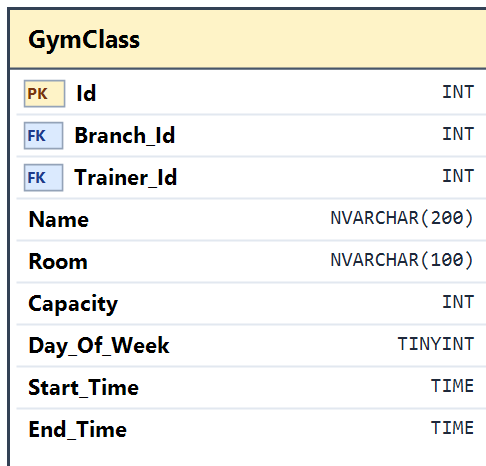
\includegraphics[width=0.34\textwidth]{images/tbl_GymClass.png}
\end{figure}
\begin{table}[H]\centering\footnotesize
\begin{tabularx}{\textwidth}{|c|L{3.0cm}|L{2.8cm}|L{3.8cm}|Y|}
\hline \textbf{STT} & \textbf{Tên thuộc tính} & \textbf{Kiểu} & \textbf{Ràng buộc} & \textbf{Ý nghĩa / Ghi chú} \\ \hline
1 & \texttt{Id} & \texttt{INT} & PK, NN, tự tăng & Mã lớp \\ \hline
2 & \texttt{Branch\_Id} & \texttt{INT} & FK $\rightarrow$ \texttt{Branches(Id)}, NN & Chi nhánh tổ chức lớp \\ \hline
3 & \texttt{Trainer\_Id} & \texttt{INT} & FK $\rightarrow$ \texttt{Trainers(Id)}, NN & HLV phụ trách \\ \hline
4 & \texttt{Name} & \texttt{NVARCHAR(200)} & NN & Tên lớp \\ \hline
5 & \texttt{Room} & \texttt{NVARCHAR(100)} & & Phòng tập \\ \hline
6 & \texttt{Capacity} & \texttt{INT} & NN, CHECK $> 0$ & Sức chứa tối đa \\ \hline
7 & \texttt{Day\_Of\_Week} & \texttt{TINYINT} & CHECK 1--7 & Thứ trong tuần của lịch lặp \\ \hline
8 & \texttt{Start\_Time} & \texttt{TIME} & & Giờ bắt đầu \\ \hline
9 & \texttt{End\_Time} & \texttt{TIME} & & Giờ kết thúc \\ \hline
\end{tabularx}
\end{table}

\subsubsection{Trainer\_Availabilities -- Lịch rảnh của HLV}
\begin{figure}[H]
\centering
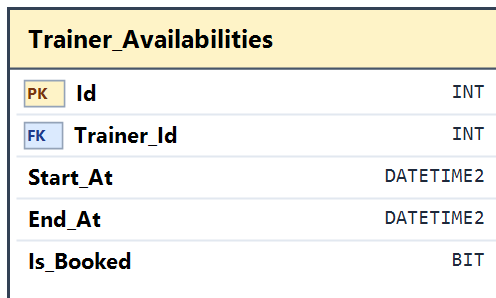
\includegraphics[width=0.34\textwidth]{images/tbl_Trainer_Availabilities.png}
\end{figure}
\begin{table}[H]\centering\footnotesize
\begin{tabularx}{\textwidth}{|c|L{3.0cm}|L{2.8cm}|L{3.8cm}|Y|}
\hline \textbf{STT} & \textbf{Tên thuộc tính} & \textbf{Kiểu} & \textbf{Ràng buộc} & \textbf{Ý nghĩa / Ghi chú} \\ \hline
1 & \texttt{Id} & \texttt{INT} & PK, NN, tự tăng & Mã khung giờ rảnh \\ \hline
2 & \texttt{Trainer\_Id} & \texttt{INT} & FK $\rightarrow$ \texttt{Trainers(Id)}, NN & HLV \\ \hline
3 & \texttt{Start\_At} & \texttt{DATETIME2} & NN & Thời điểm bắt đầu \\ \hline
4 & \texttt{End\_At} & \texttt{DATETIME2} & NN, CHECK $>$ \texttt{Start\_At} & Thời điểm kết thúc \\ \hline
5 & \texttt{Is\_Booked} & \texttt{BIT} & NN, DF \texttt{0} & Đã có người đặt hay chưa \\ \hline
\end{tabularx}
\end{table}

\subsubsection{Class\_Sessions -- Buổi học cụ thể}
\begin{figure}[H]
\centering
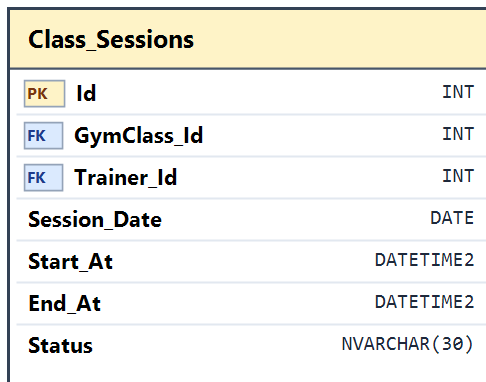
\includegraphics[width=0.34\textwidth]{images/tbl_Class_Sessions.png}
\end{figure}
\begin{table}[H]\centering\footnotesize
\begin{tabularx}{\textwidth}{|c|L{3.0cm}|L{2.8cm}|L{3.8cm}|Y|}
\hline \textbf{STT} & \textbf{Tên thuộc tính} & \textbf{Kiểu} & \textbf{Ràng buộc} & \textbf{Ý nghĩa / Ghi chú} \\ \hline
1 & \texttt{Id} & \texttt{INT} & PK, NN, tự tăng & Mã buổi học \\ \hline
2 & \texttt{GymClass\_Id} & \texttt{INT} & FK $\rightarrow$ \texttt{GymClass(Id)}, NN & Lớp tập mà buổi học thuộc về \\ \hline
3 & \texttt{Trainer\_Id} & \texttt{INT} & FK $\rightarrow$ \texttt{Trainers(Id)}, NN & HLV dạy buổi này \\ \hline
4 & \texttt{Session\_Date} & \texttt{DATE} & NN & Ngày diễn ra \\ \hline
5 & \texttt{Start\_At} & \texttt{DATETIME2} & NN & Thời điểm bắt đầu \\ \hline
6 & \texttt{End\_At} & \texttt{DATETIME2} & NN, CHECK $>$ \texttt{Start\_At} & Thời điểm kết thúc \\ \hline
7 & \texttt{Status} & \texttt{NVARCHAR(30)} & NN, DF \texttt{'Scheduled'} & Trạng thái buổi học \\ \hline
\end{tabularx}
\end{table}

\subsubsection{Notifications -- Thông báo}
\begin{figure}[H]
\centering
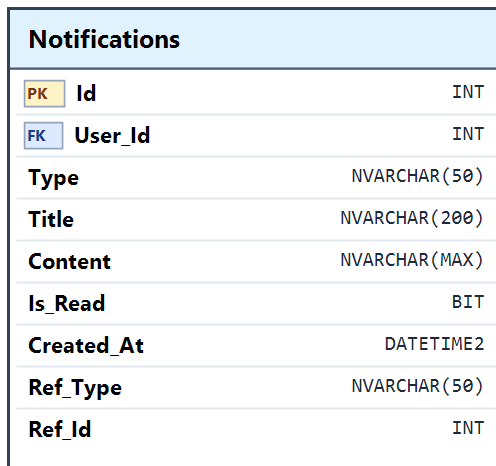
\includegraphics[width=0.34\textwidth]{images/tbl_Notifications.png}
\end{figure}
\begin{table}[H]\centering\footnotesize
\begin{tabularx}{\textwidth}{|c|L{3.0cm}|L{2.8cm}|L{3.8cm}|Y|}
\hline \textbf{STT} & \textbf{Tên thuộc tính} & \textbf{Kiểu} & \textbf{Ràng buộc} & \textbf{Ý nghĩa / Ghi chú} \\ \hline
1 & \texttt{Id} & \texttt{INT} & PK, NN, tự tăng & Mã thông báo \\ \hline
2 & \texttt{User\_Id} & \texttt{INT} & FK $\rightarrow$ \texttt{Users(Id)}, NN & Người nhận \\ \hline
3 & \texttt{Type} & \texttt{NVARCHAR(50)} & & Loại thông báo \\ \hline
4 & \texttt{Title} & \texttt{NVARCHAR(200)} & & Tiêu đề \\ \hline
5 & \texttt{Content} & \texttt{NVARCHAR(MAX)} & & Nội dung \\ \hline
6 & \texttt{Is\_Read} & \texttt{BIT} & NN, DF \texttt{0} & Đã đọc hay chưa \\ \hline
7 & \texttt{Created\_At} & \texttt{DATETIME2} & NN, DF hiện tại & Thời điểm tạo \\ \hline
8 & \texttt{Ref\_Type} & \texttt{NVARCHAR(50)} & & Loại đối tượng liên quan (Booking, Payment) \\ \hline
9 & \texttt{Ref\_Id} & \texttt{INT} & & Mã đối tượng liên quan (đa hình) \\ \hline
\end{tabularx}
\end{table}

\subsubsection{Membership\_Plans -- Gói tập}
\begin{figure}[H]
\centering
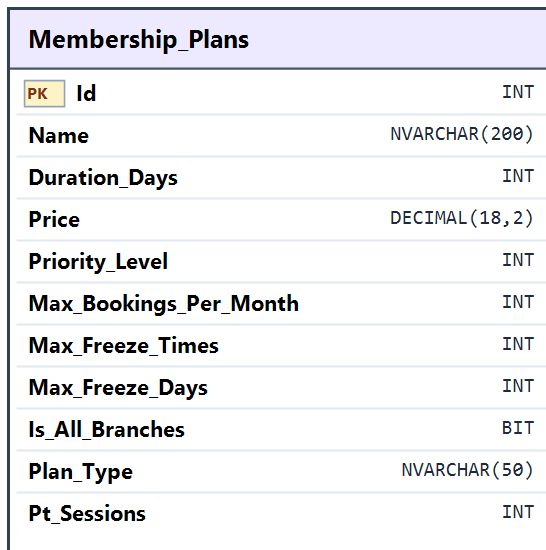
\includegraphics[width=0.34\textwidth]{images/tbl_Membership_Plans.png}
\end{figure}
\begin{table}[H]\centering\footnotesize
\begin{tabularx}{\textwidth}{|c|L{3.6cm}|L{2.6cm}|L{3.0cm}|Y|}
\hline \textbf{STT} & \textbf{Tên thuộc tính} & \textbf{Kiểu} & \textbf{Ràng buộc} & \textbf{Ý nghĩa / Ghi chú} \\ \hline
1 & \texttt{Id} & \texttt{INT} & PK, NN, tự tăng & Mã gói \\ \hline
2 & \texttt{Name} & \texttt{NVARCHAR(200)} & NN & Tên gói \\ \hline
3 & \texttt{Duration\_Days} & \texttt{INT} & NN, CHECK $> 0$ & Thời hạn (ngày) \\ \hline
4 & \texttt{Price} & \texttt{DECIMAL(18,2)} & NN, CHECK $\ge 0$ & Giá gói \\ \hline
5 & \texttt{Priority\_Level} & \texttt{INT} & NN, DF \texttt{0} & Mức ưu tiên (dùng cho hàng chờ) \\ \hline
6 & \texttt{Max\_Bookings\_Per\_Month} & \texttt{INT} & & Số lượt đặt lịch tối đa mỗi tháng \\ \hline
7 & \texttt{Max\_Freeze\_Times} & \texttt{INT} & NN, DF \texttt{0} & Số lần bảo lưu tối đa \\ \hline
8 & \texttt{Max\_Freeze\_Days} & \texttt{INT} & NN, DF \texttt{0} & Số ngày bảo lưu tối đa \\ \hline
9 & \texttt{Is\_All\_Branches} & \texttt{BIT} & NN, DF \texttt{0} & 1 = dùng được ở mọi chi nhánh \\ \hline
10 & \texttt{Plan\_Type} & \texttt{NVARCHAR(50)} & & Loại gói (thường / PT / ...) \\ \hline
11 & \texttt{Pt\_Sessions} & \texttt{INT} & NN, DF \texttt{0} & Số buổi PT kèm theo gói \\ \hline
\end{tabularx}
\end{table}

\subsubsection{Plan\_Branches -- Gói tập áp dụng tại chi nhánh}
\begin{figure}[H]
\centering
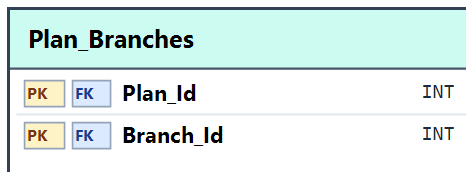
\includegraphics[width=0.34\textwidth]{images/tbl_Plan_Branches.png}
\end{figure}
\begin{table}[H]\centering\footnotesize
\begin{tabularx}{\textwidth}{|c|L{3.0cm}|L{2.2cm}|L{4.8cm}|Y|}
\hline \textbf{STT} & \textbf{Tên thuộc tính} & \textbf{Kiểu} & \textbf{Ràng buộc} & \textbf{Ý nghĩa / Ghi chú} \\ \hline
1 & \texttt{Plan\_Id} & \texttt{INT} & PK, FK $\rightarrow$ \texttt{Membership\_Plans(Id)}, NN & Gói tập \\ \hline
2 & \texttt{Branch\_Id} & \texttt{INT} & PK, FK $\rightarrow$ \texttt{Branches(Id)}, NN & Chi nhánh áp dụng (khóa chính kép) \\ \hline
\end{tabularx}
\end{table}

\subsubsection{Memberships -- Gói tập đã đăng ký của hội viên}
\begin{figure}[H]
\centering
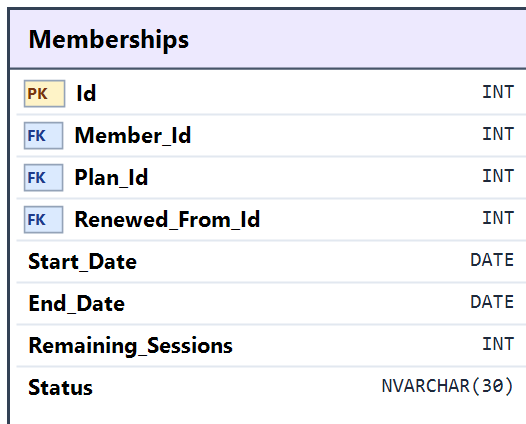
\includegraphics[width=0.34\textwidth]{images/tbl_Memberships.png}
\end{figure}
\begin{table}[H]\centering\footnotesize
\begin{tabularx}{\textwidth}{|c|L{3.2cm}|L{2.5cm}|L{4.2cm}|Y|}
\hline \textbf{STT} & \textbf{Tên thuộc tính} & \textbf{Kiểu} & \textbf{Ràng buộc} & \textbf{Ý nghĩa / Ghi chú} \\ \hline
1 & \texttt{Id} & \texttt{INT} & PK, NN, tự tăng & Mã đăng ký \\ \hline
2 & \texttt{Member\_Id} & \texttt{INT} & FK $\rightarrow$ \texttt{Members(Id)}, NN & Hội viên sở hữu \\ \hline
3 & \texttt{Plan\_Id} & \texttt{INT} & FK $\rightarrow$ \texttt{Membership\_Plans(Id)}, NN & Gói đã đăng ký \\ \hline
4 & \texttt{Renewed\_From\_Id} & \texttt{INT} & FK $\rightarrow$ \texttt{Memberships(Id)} & Gói cũ được gia hạn (NULL nếu mới) \\ \hline
5 & \texttt{Start\_Date} & \texttt{DATE} & NN & Ngày bắt đầu \\ \hline
6 & \texttt{End\_Date} & \texttt{DATE} & NN, CHECK $\ge$ \texttt{Start\_Date} & Ngày kết thúc \\ \hline
7 & \texttt{Remaining\_Sessions} & \texttt{INT} & NN, DF \texttt{0} & Số buổi PT còn lại \\ \hline
8 & \texttt{Status} & \texttt{NVARCHAR(30)} & NN, DF \texttt{'Pending\_\hspace{0pt}Payment'} & Trạng thái (\texttt{Pending\_\hspace{0pt}Payment}, \texttt{Active}, \texttt{Frozen}, \texttt{Expired}, \texttt{Cancelled}) \\ \hline
\end{tabularx}
\end{table}

\subsubsection{Payments -- Thanh toán}
\begin{figure}[H]
\centering
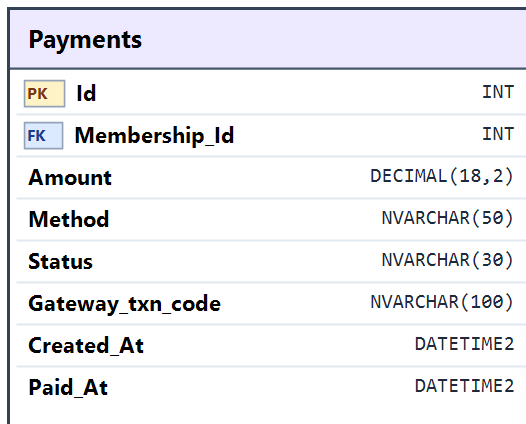
\includegraphics[width=0.34\textwidth]{images/tbl_Payments.png}
\end{figure}
\begin{table}[H]\centering\footnotesize
\begin{tabularx}{\textwidth}{|c|L{3.2cm}|L{2.6cm}|L{4.0cm}|Y|}
\hline \textbf{STT} & \textbf{Tên thuộc tính} & \textbf{Kiểu} & \textbf{Ràng buộc} & \textbf{Ý nghĩa / Ghi chú} \\ \hline
1 & \texttt{Id} & \texttt{INT} & PK, NN, tự tăng & Mã thanh toán \\ \hline
2 & \texttt{Membership\_Id} & \texttt{INT} & FK $\rightarrow$ \texttt{Memberships(Id)}, NN & Gói tập được thanh toán \\ \hline
3 & \texttt{Amount} & \texttt{DECIMAL(18,2)} & NN, CHECK $\ge 0$ & Số tiền \\ \hline
4 & \texttt{Method} & \texttt{NVARCHAR(50)} & & Phương thức thanh toán \\ \hline
5 & \texttt{Status} & \texttt{NVARCHAR(30)} & NN, DF \texttt{'Pending'} & Trạng thái giao dịch \\ \hline
6 & \texttt{Gateway\_txn\_code} & \texttt{NVARCHAR(100)} & & Mã giao dịch từ cổng thanh toán \\ \hline
7 & \texttt{Created\_At} & \texttt{DATETIME2} & NN, DF hiện tại & Thời điểm tạo giao dịch \\ \hline
8 & \texttt{Paid\_At} & \texttt{DATETIME2} & & Thời điểm thanh toán thành công \\ \hline
\end{tabularx}
\end{table}

\subsubsection{Bookings -- Đặt lịch}
\begin{figure}[H]
\centering
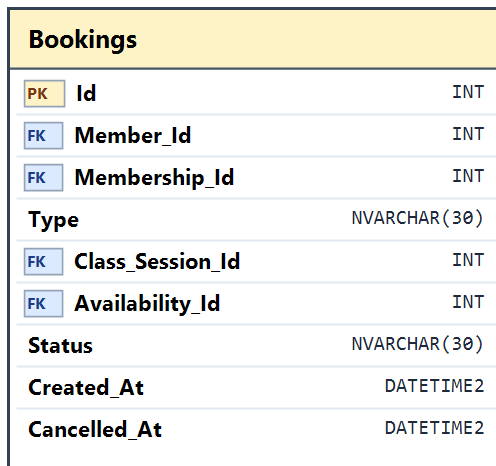
\includegraphics[width=0.34\textwidth]{images/tbl_Bookings.png}
\end{figure}
\begin{table}[H]\centering\footnotesize
\begin{tabularx}{\textwidth}{|c|L{3.2cm}|L{2.6cm}|L{4.2cm}|Y|}
\hline \textbf{STT} & \textbf{Tên thuộc tính} & \textbf{Kiểu} & \textbf{Ràng buộc} & \textbf{Ý nghĩa / Ghi chú} \\ \hline
1 & \texttt{Id} & \texttt{INT} & PK, NN, tự tăng & Mã đặt lịch \\ \hline
2 & \texttt{Member\_Id} & \texttt{INT} & FK $\rightarrow$ \texttt{Members(Id)}, NN & Hội viên đặt \\ \hline
3 & \texttt{Membership\_Id} & \texttt{INT} & FK $\rightarrow$ \texttt{Memberships(Id)}, NN & Gói tập được áp dụng \\ \hline
4 & \texttt{Type} & \texttt{NVARCHAR(30)} & NN & Loại đặt lịch: Class / PT \\ \hline
5 & \texttt{Class\_Session\_Id} & \texttt{INT} & FK $\rightarrow$ \texttt{Class\_Sessions(Id)} & Buổi lớp (khi Type = Class) \\ \hline
6 & \texttt{Availability\_Id} & \texttt{INT} & FK $\rightarrow$ \texttt{Trainer\_\hspace{0pt}Availabilities(Id)} & Khung giờ HLV (khi Type = PT) \\ \hline
7 & \texttt{Status} & \texttt{NVARCHAR(30)} & NN, DF \texttt{'Confirmed'} & Trạng thái (\texttt{Pending}, \texttt{Confirmed}, \texttt{Attended}, \texttt{Cancelled}, \texttt{Late\_\hspace{0pt}Cancelled}, \texttt{Rejected}, \texttt{No\_Show}) \\ \hline
8 & \texttt{Created\_At} & \texttt{DATETIME2} & NN, DF hiện tại & Thời điểm đặt \\ \hline
9 & \texttt{Cancelled\_At} & \texttt{DATETIME2} & & Thời điểm hủy (NULL nếu không hủy) \\ \hline
\end{tabularx}
\end{table}

\subsubsection{Checkins -- Lượt check-in}
\begin{figure}[H]
\centering
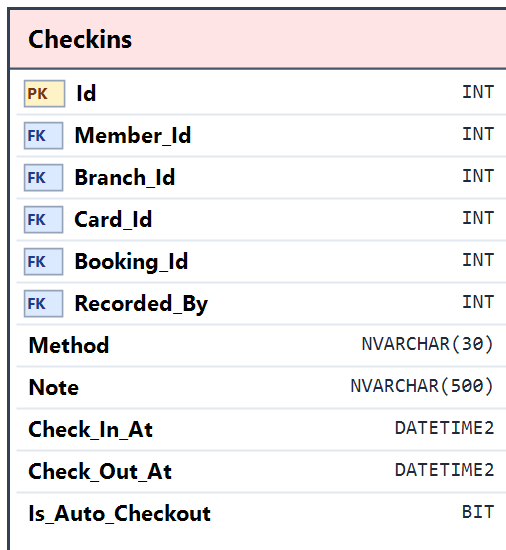
\includegraphics[width=0.34\textwidth]{images/tbl_Checkins.png}
\end{figure}
\begin{table}[H]\centering\footnotesize
\begin{tabularx}{\textwidth}{|c|L{3.2cm}|L{2.6cm}|L{4.0cm}|Y|}
\hline \textbf{STT} & \textbf{Tên thuộc tính} & \textbf{Kiểu} & \textbf{Ràng buộc} & \textbf{Ý nghĩa / Ghi chú} \\ \hline
1 & \texttt{Id} & \texttt{INT} & PK, NN, tự tăng & Mã lượt check-in \\ \hline
2 & \texttt{Member\_Id} & \texttt{INT} & FK $\rightarrow$ \texttt{Members(Id)}, NN & Hội viên check-in \\ \hline
3 & \texttt{Branch\_Id} & \texttt{INT} & FK $\rightarrow$ \texttt{Branches(Id)}, NN & Chi nhánh check-in \\ \hline
4 & \texttt{Card\_Id} & \texttt{INT} & FK $\rightarrow$ \texttt{Member\_Cards(Id)} & Thẻ sử dụng (NULL nếu nhập thủ công) \\ \hline
5 & \texttt{Booking\_Id} & \texttt{INT} & FK $\rightarrow$ \texttt{Bookings(Id)} & Lượt đặt lịch liên quan (nếu có) \\ \hline
6 & \texttt{Recorded\_By} & \texttt{INT} & FK $\rightarrow$ \texttt{Staff(Id)} & Nhân viên nhập thủ công \\ \hline
7 & \texttt{Method} & \texttt{NVARCHAR(30)} & & Hình thức check-in (thẻ/thủ công/...) \\ \hline
8 & \texttt{Note} & \texttt{NVARCHAR(500)} & & Ghi chú (lý do nhập thủ công hoặc lý do từ chối check-in) \\ \hline
9 & \texttt{Check\_In\_At} & \texttt{DATETIME2} & NN, DF hiện tại & Thời điểm vào \\ \hline
10 & \texttt{Check\_Out\_At} & \texttt{DATETIME2} & & Thời điểm ra \\ \hline
11 & \texttt{Is\_Auto\_Checkout} & \texttt{BIT} & NN, DF \texttt{0} & 1 = hệ thống tự check-out \\ \hline
\end{tabularx}
\end{table}

\subsubsection{Waitlist\_Entries -- Hàng chờ lớp}
\begin{figure}[H]
\centering
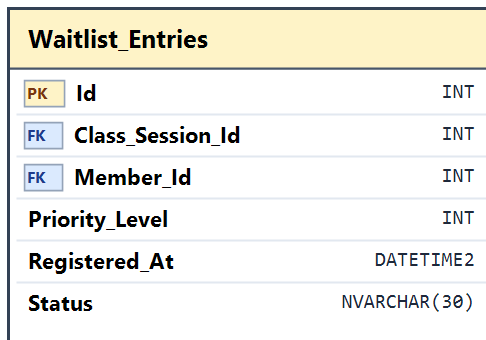
\includegraphics[width=0.34\textwidth]{images/tbl_Waitlist_Entries.png}
\end{figure}
\begin{table}[H]\centering\footnotesize
\begin{tabularx}{\textwidth}{|c|L{3.2cm}|L{2.6cm}|L{4.2cm}|Y|}
\hline \textbf{STT} & \textbf{Tên thuộc tính} & \textbf{Kiểu} & \textbf{Ràng buộc} & \textbf{Ý nghĩa / Ghi chú} \\ \hline
1 & \texttt{Id} & \texttt{INT} & PK, NN, tự tăng & Mã bản ghi hàng chờ \\ \hline
2 & \texttt{Class\_Session\_Id} & \texttt{INT} & FK $\rightarrow$ \texttt{Class\_Sessions(Id)}, NN & Buổi học đang chờ chỗ \\ \hline
3 & \texttt{Member\_Id} & \texttt{INT} & FK $\rightarrow$ \texttt{Members(Id)}, NN & Hội viên tham gia hàng chờ \\ \hline
4 & \texttt{Priority\_Level} & \texttt{INT} & NN, DF \texttt{0} & Mức ưu tiên (lấy từ gói tập) \\ \hline
5 & \texttt{Registered\_At} & \texttt{DATETIME2} & NN, DF hiện tại & Thời điểm đăng ký chờ \\ \hline
6 & \texttt{Status} & \texttt{NVARCHAR(30)} & NN, DF \texttt{'Waiting'} & Trạng thái (đang chờ/đã xếp chỗ/hủy) \\ \hline
\end{tabularx}
\end{table}

\subsubsection{Reviews -- Đánh giá}
\begin{figure}[H]
\centering
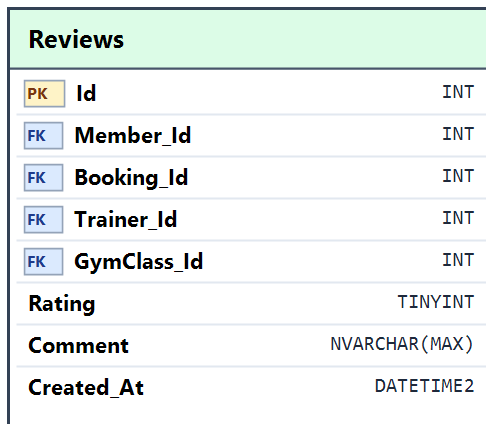
\includegraphics[width=0.34\textwidth]{images/tbl_Reviews.png}
\end{figure}
\begin{table}[H]\centering\footnotesize
\begin{tabularx}{\textwidth}{|c|L{3.0cm}|L{2.6cm}|L{4.0cm}|Y|}
\hline \textbf{STT} & \textbf{Tên thuộc tính} & \textbf{Kiểu} & \textbf{Ràng buộc} & \textbf{Ý nghĩa / Ghi chú} \\ \hline
1 & \texttt{Id} & \texttt{INT} & PK, NN, tự tăng & Mã đánh giá \\ \hline
2 & \texttt{Member\_Id} & \texttt{INT} & FK $\rightarrow$ \texttt{Members(Id)}, NN & Hội viên viết đánh giá \\ \hline
3 & \texttt{Booking\_Id} & \texttt{INT} & FK $\rightarrow$ \texttt{Bookings(Id)} & Lượt đặt lịch được đánh giá \\ \hline
4 & \texttt{Trainer\_Id} & \texttt{INT} & FK $\rightarrow$ \texttt{Trainers(Id)} & HLV được đánh giá \\ \hline
5 & \texttt{GymClass\_Id} & \texttt{INT} & FK $\rightarrow$ \texttt{GymClass(Id)} & Lớp được đánh giá \\ \hline
6 & \texttt{Rating} & \texttt{TINYINT} & NN, CHECK 1--5 & Số sao \\ \hline
7 & \texttt{Comment} & \texttt{NVARCHAR(MAX)} & & Nhận xét \\ \hline
8 & \texttt{Created\_At} & \texttt{DATETIME2} & NN, DF hiện tại & Thời điểm đánh giá \\ \hline
\end{tabularx}
\end{table}

\subsubsection{Freeze\_Requests -- Yêu cầu bảo lưu}
\begin{figure}[H]
\centering
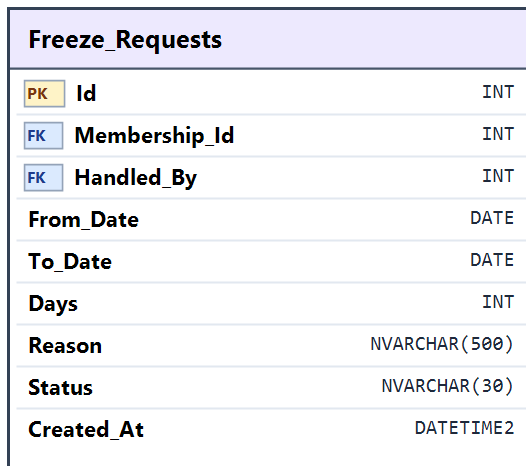
\includegraphics[width=0.34\textwidth]{images/tbl_Freeze_Requests.png}
\end{figure}
\begin{table}[H]\centering\footnotesize
\begin{tabularx}{\textwidth}{|c|L{3.2cm}|L{2.6cm}|L{4.2cm}|Y|}
\hline \textbf{STT} & \textbf{Tên thuộc tính} & \textbf{Kiểu} & \textbf{Ràng buộc} & \textbf{Ý nghĩa / Ghi chú} \\ \hline
1 & \texttt{Id} & \texttt{INT} & PK, NN, tự tăng & Mã yêu cầu \\ \hline
2 & \texttt{Membership\_Id} & \texttt{INT} & FK $\rightarrow$ \texttt{Memberships(Id)}, NN & Gói tập cần bảo lưu \\ \hline
3 & \texttt{Handled\_By} & \texttt{INT} & FK $\rightarrow$ \texttt{Staff(Id)} & Nhân viên xử lý (NULL nếu chưa duyệt) \\ \hline
4 & \texttt{From\_Date} & \texttt{DATE} & NN & Ngày bắt đầu bảo lưu \\ \hline
5 & \texttt{To\_Date} & \texttt{DATE} & NN, CHECK $\ge$ \texttt{From\_Date} & Ngày kết thúc bảo lưu \\ \hline
6 & \texttt{Days} & \texttt{INT} & NN, CHECK $> 0$ & Số ngày bảo lưu \\ \hline
7 & \texttt{Reason} & \texttt{NVARCHAR(500)} & & Lý do \\ \hline
8 & \texttt{Status} & \texttt{NVARCHAR(30)} & NN, DF \texttt{'Pending'} & Trạng thái (chờ duyệt/chấp nhận/từ chối) \\ \hline
9 & \texttt{Created\_At} & \texttt{DATETIME2} & NN, DF hiện tại & Thời điểm gửi yêu cầu \\ \hline
\end{tabularx}
\end{table}

% ==============================================================================
% 5. THIẾT KẾ KIẾN TRÚC
% ==============================================================================
\newpage
\section{Thiết kế kiến trúc}

\subsection{Architecture Drivers}
Architecture Drivers là các yêu cầu và ràng buộc quan trọng nhất có ảnh hưởng trực tiếp đến việc lựa chọn kiến trúc của hệ thống.

\begin{table}[H]
\centering
\begin{tabularx}{\textwidth}{|L{4.2cm}|Y|}
\hline
\textbf{Architecture Driver} & \textbf{Yêu cầu cụ thể của hệ thống} \\ \hline
\textbf{Chức năng chính} & Membership và freeze, waitlist theo ưu tiên hạng gói, trừ buổi PT theo nguồn (tặng kèm trừ trước, gói PT mua trừ sau), check-in kiểm tra hiệu lực gói và quyền tập chéo chi nhánh. \\ \hline
\textbf{Performance (Hiệu năng)} & Check-in phản hồi dưới 1 giây; tra cứu lịch lớp và khung giờ rảnh PT dưới 500ms. \\ \hline
\textbf{Scalability (Khả năng mở rộng)} & Mở rộng thêm nhiều chi nhánh mới; chịu tải đột biến vào khung giờ cao điểm đặt lớp (12h00, 18h00). \\ \hline
\textbf{Security (Bảo mật)} & 4 vai trò (RBAC); khóa tài khoản chặn ngay cả JWT token đang sử dụng; bảo mật toàn vẹn dữ liệu thanh toán. \\ \hline
\textbf{Availability (Độ sẵn sàng)} & Check-in tại quầy không được gián đoạn; có luồng check-in thủ công dự phòng cho lễ tân; background job chạy đúng hạn. \\ \hline
\textbf{Maintainability (Khả năng bảo trì)} & Quy tắc nghiệp vụ nhiều và hay thay đổi (mốc $T-8h$, hạn hủy lịch, giới hạn freeze, độ ưu tiên waitlist), cần cô lập khỏi framework và hạ tầng. \\ \hline
\textbf{Nền tảng công nghệ} & \textbf{Backend:} C\# (.NET 10 Web API, Modular Monolith).\newline \textbf{Frontend:} React 19 + TypeScript + Vite.\newline \textbf{Database:} Microsoft SQL Server (EF Core SqlServer). \\ \hline
\textbf{Nhân sự / Thời gian} & Nhóm 6 thành viên, phát triển song song theo từng phân hệ (module), thời gian thực hiện đồ án có hạn. \\ \hline
\textbf{Chi phí} & Sử dụng các công nghệ, framework và thư viện mã nguồn mở / miễn phí phục vụ phát triển và vận hành nội bộ. \\ \hline
\end{tabularx}
\caption{Bảng tổng hợp Architecture Drivers của hệ thống DFGymCenter}
\end{table}

\textbf{Ba Architecture Drivers quan trọng nhất:}
\begin{enumerate}
    \item \textbf{Maintainability / Modifiability:} Nghiệp vụ phức tạp và hay thay đổi, cần cô lập quy tắc nghiệp vụ khỏi framework và hạ tầng, đồng thời chia ranh giới module rõ ràng để dễ bảo trì.
    \item \textbf{Tính đúng đắn dữ liệu và bảo mật:} Thanh toán idempotent, đảm bảo ACID transaction trên SQL Server để không đặt vượt sĩ số khi nhiều người đặt cùng lúc, phân quyền chặt chẽ theo 4 vai trò.
    \item \textbf{Nhân sự / Thời gian / Chi phí:} Cần kiến trúc đủ gọn nhẹ để một nhóm nhỏ hoàn thành và vận hành đồng bộ, do đó không chọn Microservices.
\end{enumerate}

\subsection{Lựa chọn kiến trúc}
\textbf{Kiến trúc được lựa chọn (đánh dấu và mô tả):}
\begin{itemize}
    \item [$\square$] Layered / N-tier \qquad [$\boxtimes$] \textbf{Modular Monolith} \qquad [$\square$] Client-Server
    \item [$\square$] Microservices \qquad [$\square$] Event-Driven \qquad [$\square$] Serverless
    \item [$\boxtimes$] \textbf{Kết hợp bổ sung:} Áp dụng \textbf{Clean Architecture} bên trong từng module và dùng Domain Event nội bộ (MediatR).
\end{itemize}

\textbf{Mô tả ngắn kiến trúc:}
Hệ thống được đóng gói thành một khối thống nhất (\textbf{Modular Monolith}) gồm \textbf{8 module nghiệp vụ độc lập} (Bounded Contexts) được nạp vào cùng một ứng dụng host (\texttt{DFGymCenter.API}). Bên trong mỗi module, mã nguồn được tổ chức theo nguyên lý \textbf{Clean Architecture} gồm 4 tầng:
\begin{itemize}
    \item \textbf{Domain:} Chứa Entities, Value Objects, Enums và quy tắc nghiệp vụ cốt lõi của riêng module đó. Không phụ thuộc bất kỳ tầng hay module nào khác.
    \item \textbf{Application:} Chứa Use Cases (Commands/Queries qua MediatR), Validators, Interfaces và DTOs. Chỉ phụ thuộc vào Domain nội bộ và project \texttt{Contracts} công khai.
    \item \textbf{Infrastructure:} Cài đặt Repositories, DbContext riêng theo schema của module trên \textbf{Microsoft SQL Server}, cổng thanh toán và dịch vụ ngoài.
    \item \textbf{Presentation:} Tiếp nhận HTTP REST API (Controllers), xác thực JWT và chuyển yêu cầu vào Application của module tương ứng.
\end{itemize}
Các module giao tiếp với nhau thông qua \textbf{project Contracts công khai} (interfaces/DTOs) hoặc \textbf{Domain Event nội bộ}, tuyệt đối không truy cập trực tiếp vào bảng dữ liệu hoặc repository nội bộ của module khác.

\textbf{Lý do lựa chọn:}
\begin{enumerate}
    \item \textbf{Bảo vệ nghiệp vụ phức tạp:} Nghiệp vụ là phần giá trị nhất (waitlist ưu tiên, mốc $T-8h$, freeze, trừ buổi PT theo nguồn). Clean Architecture trong từng module đặt các quy tắc này ở Domain/Application, dễ viết Unit Test độc lập không cần DB hay web server.
    \item \textbf{Dễ thay thế hạ tầng:} Có thể đổi cổng thanh toán (VNPay sang ZaloPay), nhà cung cấp email hay nơi lưu trữ ảnh mà không sửa mã nguồn Use Case.
    \item \textbf{Phù hợp làm việc nhóm và bảo trì:} Ranh giới 8 module rõ ràng giúp 6 thành viên làm song song theo phân hệ không xung đột code, trong khi cấu trúc đóng gói thống nhất gọn nhẹ giúp dễ vận hành, kiểm thử và có thể nâng cấp lên Microservices trong tương lai.
\end{enumerate}

\textbf{Các hạn chế / Trade-offs:}
\begin{enumerate}
    \item Nhiều lớp và file trung gian (Contracts, DTO, Handler, Repository, Interface) nên boilerplate nhiều, đòi hỏi thời gian làm quen cao hơn Layered thông thường.
    \item Đối với các chức năng CRUD đơn giản dễ bị over-engineering nếu chia ranh giới quá nhỏ.
    \item Monolith phải scale theo cả khối; đòi hỏi kỷ luật giữ ranh giới module (kiểm tra tự động bằng \texttt{NetArchTest} trong CI).
\end{enumerate}

\subsection{Thiết kế Layer (Bên trong mỗi Module)}
Áp dụng cấu trúc 4 tầng của Clean Architecture nhất quán trong từng module của hệ thống Modular Monolith:

\begin{table}[H]
\centering
\begin{tabularx}{\textwidth}{|L{4.2cm}|Y|}
\hline
\textbf{Layer} & \textbf{Mô tả trách nhiệm \& Các thành phần chính} \\ \hline
\textbf{Presentation Layer} & Tiếp nhận HTTP Request, xác thực token, kiểm tra định dạng đầu vào cơ bản và trả kết quả JSON; tuyệt đối không chứa logic nghiệp vụ.\newline \textit{Thành phần chính:} React 19 SPA, REST Controllers (\texttt{AuthController}, \texttt{ClassesController}, \texttt{BookingsController}...), Request/Response DTOs, Middleware JWT, Exception Handling Middleware, Swagger/OpenAPI. \\ \hline
\textbf{Application Layer} & Điều phối Use Cases, xử lý validation nghiệp vụ bằng bộ tham số quy tắc (\texttt{BusinessRuleOptions} nạp từ \texttt{appsettings.json} thay vì lưu bảng CSDL riêng), quản lý transaction và phát Domain Events.\newline \textit{Thành phần chính:} Command/Query Handlers qua MediatR (\texttt{RegisterClassHandler}, \texttt{CancelBookingHandler}, \texttt{ApproveFreezeHandler}...), FluentValidation, \texttt{IOptions<BusinessRuleOptions>}, Interfaces (\texttt{IBookingRepository}, \texttt{IPaymentGateway}), Module Contracts. \\ \hline
\textbf{Domain Layer} & Nắm giữ thực thể cốt lõi, trạng thái và các quy tắc bất biến (Business Invariants) của module.\newline \textit{Thành phần chính:} Entities (\texttt{Membership}, \texttt{Booking}, \texttt{ClassSession}, \texttt{WaitlistEntry}...), Enums, Domain Events (\texttt{BookingConfirmedEvent}, \texttt{FreezeApprovedEvent}), Domain Exceptions. \\ \hline
\textbf{Infrastructure Layer} & Kết nối CSDL Microsoft SQL Server, thực thi truy vấn, mapping dữ liệu và tích hợp dịch vụ hạ tầng bên ngoài.\newline \textit{Thành phần chính:} EF Core \texttt{DbContext} theo schema riêng của từng module, Repository Implementations, Unit of Work, Payment Gateway Client, Email/SMTP Sender, Cloudinary Client, Hangfire Jobs (\texttt{Hangfire.SqlServer}). \\ \hline
\end{tabularx}
\caption{Mô tả trách nhiệm 4 tầng Clean Architecture trong mỗi Module}
\end{table}

\textbf{Quy tắc phụ thuộc (Dependency Rule) giữa các tầng và module:}
\begin{itemize}
    \item Tầng \textbf{Domain} không tham chiếu bất kỳ tầng hay module nào khác.
    \item Tầng \textbf{Application} chỉ tham chiếu tầng \textbf{Domain} của module đó và các \textbf{Module Contracts} công khai.
    \item Tầng \textbf{Infrastructure} tham chiếu \textbf{Application} và \textbf{Domain} để cài đặt các interface đã định nghĩa.
    \item Project khởi chạy \textbf{DFGymCenter.API} (Composition Root) tham chiếu các module để đăng ký Dependency Injection, cấu hình middleware và cung cấp Endpoint thống nhất.
\end{itemize}

\subsection{Phân chia Module / Subsystem}
9 nhóm chức năng nghiệp vụ ở Phần 1 được tổ chức thành \textbf{8 module theo nghiệp vụ} (Bounded Context, trong đó chức năng Lớp học nhóm và Lịch PT 1-kèm-1 được gộp chung vào module \textit{Scheduling}), không chia theo vai trò người dùng; mỗi module làm chủ hoàn toàn schema/bảng dữ liệu của mình trên SQL Server.

\begin{table}[H]
\centering
\begin{tabularx}{\textwidth}{|L{4.2cm}|Y|L{4.2cm}|}
\hline
\textbf{Module / Subsystem} & \textbf{Trách nhiệm chính} & \textbf{Dữ liệu sở hữu (Tables)} \\ \hline
\textbf{Identity \& Account} & Đăng ký, đăng nhập, cấp JWT, phân quyền RBAC, khóa/mở khóa tài khoản, hồ sơ hội viên/HLV/lễ tân, thẻ hội viên. & \texttt{Users}, \texttt{Members}, \texttt{Trainers}, \texttt{Staff}, \texttt{Member\_Cards} \\ \hline
\textbf{Membership \& Payment} & Danh mục gói, phạm vi chi nhánh áp dụng của gói (tập chéo), mua/gia hạn gói hội viên và gói PT, duyệt freeze, quản lý buổi PT tặng kèm, thanh toán online, lịch sử giao dịch. & \texttt{Membership\_Plans}, \texttt{Plan\_Branches}, \texttt{Memberships}, \texttt{Freeze\_Requests}, \texttt{Payments} \\ \hline
\textbf{Branch \& Equipment} & Quản lý thông tin chi nhánh và giờ mở/đóng cửa, danh mục máy tập, tiếp nhận và xử lý sự cố thiết bị. & \texttt{Branches}, \texttt{Equipment}, \texttt{Equipment\_Issues}, \texttt{Equipment\_Issues\_Logs} \\ \hline
\textbf{Scheduling (Class \& PT)} & Quản lý lớp nhóm, buổi học cụ thể, đăng ký/hủy lịch, danh sách chờ waitlist, lịch rảnh PT, đặt lịch PT 1-kèm-1, điểm danh. & \texttt{GymClass}, \texttt{Class\_Sessions}, \texttt{Bookings}, \texttt{Waitlist\_Entries}, \texttt{Trainer\_Availabilities} \\ \hline
\textbf{Access Control (Check-in)} & Check-in/check-out bằng thẻ/QR hoặc thủ công, đối soát hiệu lực gói và chi nhánh, tự check-out lúc đóng cửa. & \texttt{Checkins} \\ \hline
\textbf{Progress \& Review} & Lưu trữ chỉ số cơ thể, lịch sử đo theo mốc thời gian, biểu đồ tiến độ, đánh giá PT và lớp học. & \texttt{Body\_Metrics}, \texttt{Reviews} \\ \hline
\textbf{Notification} & Tạo, gửi, đánh dấu đã đọc thông báo hệ thống, gửi nhắc lịch học và cảnh báo sắp hết hạn gói. & \texttt{Notifications} \\ \hline
\textbf{Analytics \& Reporting} & Thống kê doanh thu theo chi nhánh, tỷ lệ churn, hiệu suất lớp học và PT, kết xuất báo cáo Excel/PDF động tức thời. & Read Models / Views tổng hợp (không lưu bảng hay file báo cáo trong CSDL để tránh nặng máy) \\ \hline
\end{tabularx}
\caption{Phân chia 8 Module nghiệp vụ của hệ thống DFGymCenter}
\end{table}

\textbf{Nguyên tắc thiết kế Module:}
\begin{itemize}
    \item \textbf{High Cohesion:} Các chức năng và thực thể cùng một miền nghiệp vụ nằm gọn trong một module.
    \item \textbf{Low Coupling:} Các module chỉ giao tiếp thông qua \texttt{Contracts} (Interface, DTO, Integration Event), tuyệt đối không join bảng trực tiếp chéo schema hoặc gọi thẳng Repository của module khác.
    \item \textbf{Tránh Circular Dependency:} \textit{Scheduling} gọi \textit{Membership \& Payment} qua interface để kiểm tra/trừ buổi; ngược lại khi freeze được duyệt, \textit{Membership \& Payment} phát Domain Event \texttt{FreezeApprovedEvent} để \textit{Scheduling} tự động hủy lịch mà không tham chiếu ngược.
\end{itemize}

\subsection{Giao tiếp giữa các Module}
Giao tiếp đồng bộ dùng lời gọi Interface trong cùng process (\texttt{Contracts}); giao tiếp bất đồng bộ dùng Domain Event nội bộ (\textbf{MediatR}) và job nền (\textbf{Hangfire.SqlServer}).

\begin{table}[H]
\centering
\footnotesize
\begin{tabularx}{\textwidth}{|L{2.5cm}|L{2.5cm}|L{2.8cm}|Y|L{2.8cm}|}
\hline
\textbf{Module nguồn} & \textbf{Module đích} & \textbf{Dữ liệu quản lý} & \textbf{Nội dung trao đổi} & \textbf{Hình thức} \\ \hline
Access Control (Check-in) & Identity \& Account & \texttt{CardCode}, \texttt{UserId}, \texttt{UserStatus} & Tra cứu thông tin chủ thẻ từ mã QR/thẻ từ và kiểm tra tài khoản không bị khóa khi check-in. & \textbf{Đồng bộ}\newline Contract Interface (\texttt{IIdentityContract}) \\ \hline
Access Control (Check-in) & Membership \& Payment & \texttt{MemberId}, \texttt{MembershipStatus}, \texttt{EndDate}, \texttt{PlanBranches} & Kiểm tra gói hội viên còn hiệu lực, không đang freeze và kiểm tra quyền tập chéo tại chi nhánh hiện tại (\texttt{Plan\_Branches}). & \textbf{Đồng bộ}\newline Contract Interface (\texttt{IMembershipContract}) \\ \hline
Access Control (Check-in) & Branch \& Equipment & \texttt{BranchId}, \texttt{BranchStatus}, \texttt{OpenCloseTime} & Kiểm tra chi nhánh hiện tại đang hoạt động (\texttt{Active}) và trong khung giờ mở cửa hợp lệ khi check-in. & \textbf{Đồng bộ}\newline Contract Interface (\texttt{IBranchContract}) \\ \hline
Scheduling (Class \& PT) & Membership \& Payment & \texttt{MembershipId}, \texttt{RemainingSessions} & Kiểm tra gói còn hạn, đúng chi nhánh, còn buổi PT khả dụng; thực hiện trừ hoặc hoàn lại buổi tập. & \textbf{Đồng bộ}\newline Contract Interface (\texttt{IMembershipContract}) \\ \hline
Membership \& Payment & Cổng thanh toán (VNPay / ZaloPay) & \texttt{OrderId}, \texttt{Amount}, \texttt{TransactionId}, \texttt{Signature} & Tạo URL giao dịch thanh toán online; tiếp nhận callback IPN kiểm tra chữ ký và kích hoạt gói. & \textbf{Bất đồng bộ}\newline HTTP Redirect \& Webhook IPN \\ \hline
Membership \& Payment & Scheduling (Class \& PT) & \texttt{MemberId}, \texttt{FreezeStartDate}, \texttt{FreezeEndDate} & Phát event \texttt{FreezeApprovedEvent} để Scheduling tự động hủy lịch tập trong khoảng freeze và hoàn buổi. & \textbf{Bất đồng bộ}\newline MediatR Domain Event \\ \hline
Scheduling (Class \& PT) & Scheduling (Xử lý nội bộ) & \texttt{ClassSessionId}, \texttt{WaitlistEntryId}, \texttt{Priority} & Phát event nội bộ \texttt{BookingCancelledEvent} để đôn người đứng đầu waitlist lên đặt chỗ chính thức. & \textbf{Bất đồng bộ}\newline Internal Domain Event \\ \hline
Access Control (Check-in) & Scheduling (Class \& PT) & \texttt{MemberId}, \texttt{BranchId}, \texttt{CheckinTime} & Phát event \texttt{CheckinValidatedEvent} để tự động gắn cờ đã check-in (\texttt{CheckedIn}) cho các lịch lớp/PT trong ngày làm cơ sở để HLV xác nhận điểm danh (\texttt{Attended}/\texttt{Completed}). & \textbf{Bất đồng bộ}\newline MediatR Domain Event \\ \hline
Scheduling (Class \& PT) & Progress \& Review & \texttt{BookingId}, \texttt{MemberId}, \texttt{TrainerId} & Phát event \texttt{SessionCompletedEvent} sau khi PT xác nhận hoàn thành buổi tập để mở quyền đánh giá. & \textbf{Bất đồng bộ}\newline MediatR Domain Event \\ \hline
Hầu hết các Module & Notification & \texttt{UserId}, \texttt{Title}, \texttt{Content}, \texttt{Type} & Lắng nghe các event thanh toán, duyệt freeze, đặt/hủy lịch, sự cố thiết bị để tạo và gửi thông báo. & \textbf{Bất đồng bộ}\newline Event Handler / Hangfire Job \\ \hline
Analytics \& Reporting & Tất cả Module nghiệp vụ & \texttt{Revenue}, \texttt{CheckinStats}, \texttt{FillRate} & Truy vấn tổng hợp (Read-only DTO/View) phục vụ báo cáo doanh thu, tỷ lệ lấp đầy và hiệu suất HLV. & \textbf{Đồng bộ}\newline Read-only Query Contract \\ \hline
\end{tabularx}
\caption{Bảng chi tiết giao tiếp giữa các Module}
\end{table}

\textbf{Job nền (Hangfire với SQL Server -- đọc ngưỡng tham số từ \texttt{BusinessRuleOptions} trong \texttt{appsettings.json}):}
\begin{itemize}
    \item Đóng danh sách chờ (waitlist) ở mốc $T-8h$ trước giờ lớp học bắt đầu.
    \item Tự động check-out toàn bộ hội viên còn trong phòng tập lúc đóng cửa chi nhánh (22h00).
    \item Nhắc lịch tập tự động trước giờ học (mặc định 2 giờ theo \texttt{BusinessRuleOptions}).
    \item Quét chuyển trạng thái gói sang \texttt{Expired}/\texttt{Frozen} và gửi cảnh báo gói sắp hết hạn.
\end{itemize}

\subsection{Thiết kế dữ liệu}
\textbf{Hệ quản trị CSDL sử dụng:}
\begin{itemize}
    \item [$\square$] PostgreSQL \qquad [$\square$] MySQL \qquad [$\boxtimes$] \textbf{SQL Server (Microsoft SQL Server / LocalDB)} \qquad [$\square$] Khác: ..........................
\end{itemize}

\textbf{Tổ chức dữ liệu theo Module trên SQL Server:}
Dữ liệu được lưu trữ tập trung trên một database instance \texttt{DFGymCenterDb} để đảm bảo giao dịch ACID, nhưng phân tách logic theo từng schema/nhóm bảng thuộc quyền sở hữu của từng module:
\begin{itemize}
    \item \textbf{Identity \& Account:} \texttt{Users}, \texttt{Members}, \texttt{Trainers}, \texttt{Staff}, \texttt{Member\_Cards}.
    \item \textbf{Membership \& Payment:} \texttt{Membership\_Plans}, \texttt{Plan\_Branches}, \texttt{Memberships}, \texttt{Freeze\_Requests}, \texttt{Payments}.
    \item \textbf{Branch \& Equipment:} \texttt{Branches}, \texttt{Equipment}, \texttt{Equipment\_Issues}, \texttt{Equipment\_Issues\_Logs}.
    \item \textbf{Scheduling (Class \& PT):} \texttt{GymClass}, \texttt{Class\_Sessions}, \texttt{Bookings}, \texttt{Waitlist\_Entries}, \texttt{Trainer\_Availabilities}.
    \item \textbf{Access Control:} \texttt{Checkins}.
    \item \textbf{Progress \& Review:} \texttt{Body\_Metrics} (giữ mốc ban đầu \texttt{Is\_Initial = 1}, không ghi đè), \texttt{Reviews}.
    \item \textbf{Notification:} \texttt{Notifications}.
\end{itemize}

\subsection{Hệ thống / Dịch vụ bên ngoài}

\begin{table}[H]
\centering
\begin{tabularx}{\textwidth}{|L{4.2cm}|L{4.5cm}|Y|}
\hline
\textbf{External System} & \textbf{Mục đích} & \textbf{Cách tích hợp} \\ \hline
\textbf{Cổng thanh toán (VNPay / ZaloPay)} & Thanh toán online khi mua hoặc gia hạn gói tập. & Redirect sang cổng thanh toán; tiếp nhận callback/IPN, kiểm tra chữ ký HMAC-SHA512, xử lý idempotent. \\ \hline
\textbf{Email / SMS / Push Service (SendGrid / SMTP)} & Gửi thông tin đăng nhập, mã OTP khôi phục mật khẩu, thông báo nhắc lịch. & Tích hợp qua REST API hoặc SMTP thông qua interface \texttt{INotificationSender} / \texttt{IEmailService}. \\ \hline
\textbf{Đầu đọc thẻ / Camera QR tại cổng} & Quét mã thẻ hoặc QR hội viên khi check-in/check-out. & Gửi chuỗi mã thẻ tới REST API endpoint \texttt{/api/checkins}. \\ \hline
\textbf{Cloudinary (Cloud Storage -- tùy chọn mở rộng)} & Lưu trữ tệp ảnh đại diện (avatar) hoặc ảnh sự cố thiết bị tách khỏi CSDL quan hệ chính để tránh nặng bảng lõi. & Tích hợp SDK/REST API khi bật lưu trữ đa phương tiện ngoài luồng giao dịch chính. \\ \hline
\textbf{Microsoft SQL Server} & CSDL chính lưu trữ toàn bộ dữ liệu giao dịch và nghiệp vụ. & Kết nối qua giao thức TDS / ADO.NET bằng Entity Framework Core SqlServer Provider. \\ \hline
\end{tabularx}
\caption{Bảng tích hợp hệ thống và dịch vụ bên ngoài}
\end{table}

\subsection{Sơ đồ kiến trúc tổng thể}

\begin{figure}[H]
\centering
\resizebox{\textwidth}{!}{
\begin{tikzpicture}[
    node distance=0.8cm and 0.8cm,
    box/.style={rectangle, draw=navyblue, fill=white, rounded corners=3pt, thick, align=center, font=\small, inner sep=5pt},
    mod/.style={rectangle, draw=navyblue!80, fill=blue!4, rounded corners=2pt, align=center, font=\scriptsize, minimum width=3.1cm, minimum height=0.9cm},
    arrow/.style={-{Stealth[scale=0.9]}, thick, navyblue}
]

\node[box, fill=navyblue!10, minimum width=12cm] (users) at (0, 0) {\textbf{Người dùng hệ thống:} Hội viên $\cdot$ Huấn luyện viên (PT) $\cdot$ Nhân viên lễ tân $\cdot$ Admin};
\node[box, fill=blue!5, minimum width=12cm, below=0.7cm of users] (client) {\textbf{Client Layer (Frontend)}: React 19 SPA (Web 4 vai trò) \quad $\mid$ \quad Đầu đọc thẻ / Kiosk QR tại cổng};
\node[box, fill=green!5, minimum width=13.5cm, below=0.8cm of client] (pres) {\textbf{Host Entry Point (DFGymCenter.API -- Presentation Layer)}\\REST Controllers $\cdot$ JWT Auth Middleware $\cdot$ Validation $\cdot$ Swagger/OpenAPI};

\node[mod, below=0.8cm of pres, xshift=-5.1cm] (m1) {\textbf{Identity \& Account}\\(Clean Arch 4 tầng)};
\node[mod, right=0.25cm of m1] (m2) {\textbf{Membership \& Payment}\\(Clean Arch 4 tầng)};
\node[mod, right=0.25cm of m2] (m3) {\textbf{Branch \& Equipment}\\(Clean Arch 4 tầng)};
\node[mod, right=0.25cm of m3] (m4) {\textbf{Scheduling (Class \& PT)}\\(Clean Arch 4 tầng)};

\node[mod, below=0.35cm of m1] (m5) {\textbf{Access Control}\\(Clean Arch 4 tầng)};
\node[mod, right=0.25cm of m5] (m6) {\textbf{Progress \& Review}\\(Clean Arch 4 tầng)};
\node[mod, right=0.25cm of m6] (m7) {\textbf{Notification}\\(Clean Arch 4 tầng)};
\node[mod, right=0.25cm of m7] (m8) {\textbf{Analytics \& Reporting}\\(Read-only Queries)};

\node[below=0.2cm of m6, xshift=1.7cm, font=\scriptsize\itshape, text=navyblue] (comm) {Giao tiếp đồng bộ qua \textbf{Contracts} \& bất đồng bộ qua \textbf{Domain Events (MediatR)} + \textbf{Hangfire Jobs}};

\begin{scope}[on background layer]
    \node[rectangle, draw=gray!80, fill=yellow!5, dashed, rounded corners=5pt, inner sep=8pt, fit=(m1)(m4)(m5)(m8)(comm)] (monolith_box) {};
\end{scope}

\node[box, fill=purple!6, minimum width=13.5cm, below=0.7cm of monolith_box] (infra) {\textbf{Data Access \& Integration (Module Infrastructure)}\\EF Core SqlServer (Schema riêng từng module) $\cdot$ Hangfire.SqlServer $\cdot$ Payment/Email/Storage Clients};
\node[box, fill=red!10, minimum width=6.4cm, below=0.9cm of infra, xshift=-3.5cm] (db) {\textbf{Database: Microsoft SQL Server}\\Database \texttt{DFGymCenterDb} (ACID Transactions)};
\node[box, fill=cyan!6, minimum width=6.4cm, below=0.9cm of infra, xshift=3.5cm] (ext) {\textbf{Dịch vụ bên ngoài}\\VNPay/ZaloPay $\cdot$ Email (SMTP)};

\draw[arrow] (users) -- node[right, font=\scriptsize] {Tương tác} (client);
\draw[arrow] (client) -- node[right, font=\scriptsize] {HTTPS / JSON + JWT Bearer} (pres);
\draw[arrow] (pres) -- node[right, font=\scriptsize] {Dispatch Command/Query (MediatR)} (monolith_box);
\draw[arrow] (monolith_box) -- node[right, font=\scriptsize] {Implements Interfaces} (infra);
\draw[arrow] (infra.south -| db.north) -- node[left, font=\scriptsize] {ADO.NET / TDS} (db.north);
\draw[arrow] (infra.south -| ext.north) -- node[right, font=\scriptsize] {REST API / Webhook} (ext.north);

\end{tikzpicture}
}
\caption{Sơ đồ kiến trúc tổng thể Modular Monolith kết hợp Clean Architecture}
\end{figure}

\subsection{Luồng xử lý minh họa}
\textbf{Use Case được chọn:} \textbf{Hội viên đăng ký lớp học nhóm (có waitlist và kiểm tra mốc $T-8h$)}, vì luồng này đi xuyên qua nhiều tầng Clean Architecture và nhiều module.

\begin{enumerate}
    \item Hội viên bấm nút \textbf{"Đăng ký"} trên React; ứng dụng gửi request \texttt{POST /api/class-sessions/\{id\}/register} kèm JWT Bearer Token.
    \item \texttt{ClassesController} (tầng Presentation thuộc module \textit{Scheduling}) xác thực JWT token, kiểm tra định dạng cơ bản, khởi tạo \texttt{RegisterClassCommand} và gửi qua MediatR.
    \item \texttt{RegisterClassHandler} (tầng Application của \textit{Scheduling}) gọi sang module \textit{Membership \& Payment} thông qua interface \texttt{IMembershipContract} để kiểm tra: gói tập còn hạn, không bị freeze, đúng chi nhánh (hoặc có quyền tập chéo), và còn lượt đặt.
    \item Handler tải thực thể \texttt{ClassSession} từ \texttt{ISessionRepository} (sử dụng khóa bản ghi mức giao dịch trong SQL Server Transaction để chống tranh chấp đồng thời) và gọi hàm \texttt{session.Register()} trong tầng Domain của \textit{Scheduling}: kiểm tra sĩ số, kiểm tra trùng lịch và đối soát mốc thời gian $T-8h$.
    \item \textbf{Xử lý kết quả trong SQL Server Transaction:}
    \begin{itemize}
        \item \textit{Còn chỗ:} Tạo bản ghi \texttt{Booking} (trạng thái \texttt{Confirmed}) và tăng số lượng học viên đã đăng ký trong cùng một transaction.
        \item \textit{Hết chỗ và còn hơn 8 giờ ($> T-8h$):} Tạo bản ghi \texttt{WaitlistEntry} theo thứ tự ưu tiên hạng gói.
        \item \textit{Hết chỗ và dưới 8 giờ ($< T-8h$):} Từ chối đăng ký vì danh sách chờ đã đóng, thông báo chọn buổi học khác.
    \end{itemize}
    \item Handler phát Domain Event \texttt{BookingConfirmedEvent} hoặc \texttt{WaitlistJoinedEvent}; module \textit{Notification} lắng nghe bất đồng bộ để gửi thông báo xác nhận, Controller trả kết quả \texttt{200 OK} về React cập nhật giao diện.
\end{enumerate}

\subsection{Bảo mật}
\begin{itemize}
    \item \textbf{Authentication (Xác thực):} Đăng nhập bằng Email/SĐT và mật khẩu (băm bằng BCrypt hoặc PBKDF2); backend cấp phát JWT chứa \texttt{UserId}, \texttt{Role} (và \texttt{BranchId} đối với tài khoản Lễ tân trực thuộc chi nhánh). Middleware kiểm tra trạng thái tài khoản \texttt{Users.Status} ở mỗi request (kết hợp cache ngắn bằng \texttt{IMemoryCache}), đảm bảo tài khoản bị khóa bị chặn ngay cả khi token vẫn còn hạn. Hỗ trợ giới hạn số lần đăng nhập sai và quên mật khẩu qua OTP/link đặt lại.
    \item \textbf{Authorization (Phân quyền):} Phân quyền theo vai trò \textbf{RBAC (Role-Based Access Control)} với 4 vai trò:
\end{itemize}

\begin{table}[H]
\centering
\begin{tabularx}{\textwidth}{|L{3.5cm}|Y|}
\hline
\textbf{Vai trò (Role)} & \textbf{Quyền hạn chính trên hệ thống} \\ \hline
\textbf{Hội viên (Member)} & Quản lý hồ sơ và chỉ số cơ thể; mua/gia hạn gói tập, gửi yêu cầu freeze; đặt/hủy lớp nhóm và lịch PT 1-kèm-1; check-in bằng mã QR và tự báo mất thẻ; đánh giá PT/lớp học; phản ánh sự cố thiết bị; xem thông báo. \\ \hline
\textbf{Huấn luyện viên (Trainer / PT)} & Quản lý hồ sơ chuyên môn và khung giờ rảnh; xác nhận hoặc từ chối lịch hẹn 1-kèm-1; xem lịch giảng dạy; điểm danh lớp nhóm và xác nhận hoàn thành buổi PT. \\ \hline
\textbf{Lễ tân (Staff)} & Duyệt yêu cầu freeze; thực hiện check-in/check-out thủ công; cấp phát, khóa, mở khóa, báo mất và cấp lại thẻ thành viên; tra cứu hội viên và xem lịch sử check-in; tiếp nhận và cập nhật trạng thái sự cố thiết bị (trong phạm vi chi nhánh được gán). \\ \hline
\textbf{Quản trị viên (Admin)} & Toàn quyền quản trị hệ thống: quản lý tài khoản, phân quyền, khóa/mở khóa tài khoản; quản lý chi nhánh, thiết bị, gói tập, lớp học và phân công HLV; xem thống kê và xuất báo cáo doanh thu. \\ \hline
\end{tabularx}
\caption{Bảng phân quyền chi tiết theo 4 vai trò (RBAC)}
\end{table}

\begin{itemize}
    \item \textbf{Bảo vệ dữ liệu:}
    \begin{itemize}
        \item Cấu hình \textbf{CORS} chỉ cho phép origin của Frontend React (\texttt{localhost:5173}) truy cập API; khi vận hành thực tế ép buộc sử dụng \textbf{HTTPS} cho toàn bộ giao tiếp client-server.
        \item Toàn bộ khóa bí mật (JWT Secret, SQL Connection String, Payment Hash Secret) lưu trong biến môi trường hoặc tệp cấu hình bảo mật, không commit lên Git.
        \item Không lưu thông tin thẻ thanh toán trên CSDL; chỉ lưu mã giao dịch và kiểm tra chữ ký số HMAC trên toàn bộ callback/IPN thanh toán.
        \item Client (React) tuyệt đối không kết nối trực tiếp CSDL; mọi truy vấn đi qua lớp API có kiểm soát phân quyền và ghi nhật ký check-in thủ công kèm mã nhân viên thao tác.
    \end{itemize}
\end{itemize}

\subsection{Công nghệ sử dụng}

\begin{table}[H]
\centering
\begin{tabularx}{\textwidth}{|L{3.8cm}|Y|}
\hline
\textbf{Thành phần} & \textbf{Công nghệ / Thư viện sử dụng} \\ \hline
\textbf{Frontend} & React 19 + TypeScript, Vite, React Router DOM 7, Recharts, Lucide Icons. \\ \hline
\textbf{Backend} & ASP.NET Core 10 (.NET 10), Modular Monolith + Clean Architecture, MediatR, FluentValidation, EF Core SqlServer 10. \\ \hline
\textbf{Database} & Microsoft SQL Server (SQL Server / LocalDB). \\ \hline
\textbf{API} & RESTful API + Swagger / OpenAPI / Scalar. \\ \hline
\textbf{Authentication} & JWT Bearer Authentication, mật khẩu băm PBKDF2 / BCrypt. \\ \hline
\textbf{Công cụ khác} & Hangfire.SqlServer (Background Jobs), Serilog, SignalR, xUnit, NetArchTest.Rules. \\ \hline
\end{tabularx}
\caption{Bảng danh mục công nghệ sử dụng cho hệ thống DFGymCenter}
\end{table}

\subsection{Đánh giá kiến trúc}
Kiến trúc \textbf{Modular Monolith} kết hợp \textbf{Clean Architecture} bên trong từng module bảo vệ tốt phần nghiệp vụ phức tạp và phù hợp với nhóm sinh viên; đổi lại cần tuân thủ kỷ luật ranh giới module và chấp nhận lượng boilerplate ban đầu.

\subsubsection{Ưu điểm}
\begin{enumerate}
    \item Nghiệp vụ cốt lõi nằm hoàn toàn trong Domain/Application của từng module, test độc lập không cần DB hay framework.
    \item Dễ dàng thay thế hạ tầng (cổng thanh toán, dịch vụ email) mà không ảnh hưởng đến Use Case.
    \item Ranh giới module rõ ràng giúp 6 thành viên phát triển song song không giẫm chân lên nhau; đóng gói thống nhất giúp cài đặt và chạy kiểm thử nhanh gọn.
    \item Đảm bảo tính nhất quán dữ liệu tuyệt đối (ACID Transaction, Row Lock) nhờ dùng Microsoft SQL Server làm CSDL tập trung.
\end{enumerate}

\subsubsection{Hạn chế}
\begin{enumerate}
    \item Nhiều lớp và boilerplate code (Contracts, DTO, Mapper, Handler, Interface); cần kỷ luật giữ ranh giới module thông qua kiểm tra tự động bằng \texttt{NetArchTest}.
    \item \textbf{Khả năng mở rộng theo module riêng lẻ:} Do đóng gói chung một tiến trình host (\texttt{DFGymCenter.API}), toàn bộ các module sẽ mở rộng cùng nhau khi tải tăng cao thay vì scale độc lập từng dịch vụ như Microservices.
    \item \textbf{Phụ thuộc kết nối CSDL tập trung:} Toàn bộ module dùng chung một instance SQL Server, đòi hỏi tối ưu chỉ số truy vấn (index) và transaction ngắn để tránh nghẽn cổ chai dữ liệu.
\end{enumerate}

\subsubsection{Khả năng mở rộng trong tương lai}
\begin{enumerate}
    \item Tích hợp thêm bộ nhớ đệm \textbf{Redis Cache} cho các truy vấn tra cứu lịch lớp và check-in mật độ cao; nâng cấp scale nhiều instance kèm SignalR backplane.
    \item Tách các module chịu tải hoặc có đặc thù xử lý riêng (như \textit{Notification} hoặc \textit{Analytics}) thành Microservice độc lập thông qua Message Broker (RabbitMQ) và Outbox Pattern nhờ ranh giới \texttt{Contracts} đã chuẩn bị sẵn.
    \item Phát triển thêm ứng dụng di động (React Native / Flutter) tái sử dụng toàn bộ hệ thống REST API hiện có.
\end{enumerate}

% ==============================================================================
% 6. THIẾT KẾ GIAO DIỆN
% ==============================================================================
\newpage
\section{Thiết kế giao diện}

\subsection{Tổng quan và Nguyên tắc thiết kế giao diện}
Giao diện người dùng (User Interface -- UI) của hệ thống quản lý chuỗi phòng gym \textbf{DFGymCenter} được thiết kế theo kiến trúc Modular Monolith kết hợp Clean Architecture (Presentation -- Application -- Domain -- Infrastructure) tương ứng với mô hình tách biệt ranh giới (\textit{Boundary -- Control -- Entity}), bảo đảm tính trực quan, nhất quán và tối ưu trải nghiệm thao tác cho 4 nhóm vai trò: \textbf{Hội viên}, \textbf{Huấn luyện viên (PT)}, \textbf{Nhân viên Lễ tân} và \textbf{Quản trị viên}.

\subsubsection{Mục tiêu thiết kế}
Hệ thống giao diện được xây dựng nhằm đáp ứng đồng bộ 4 mục tiêu thiết kế cốt lõi được tổng hợp trong bảng dưới đây:

\begin{table}[H]
\centering
{\footnotesize
\setlength{\tabcolsep}{4pt}
\begin{tabularx}{\textwidth}{|c|L{4.5cm}|Y|}
\hline
\textbf{STT} & \textbf{Mục tiêu thiết kế} & \textbf{Nội dung áp dụng trong hệ thống DFGymCenter} \\ \hline
1 & Tính trực quan và dễ sử dụng (\textit{Usability}) & Bố cục màn hình rõ ràng, sử dụng thẻ thông tin, bảng biểu và nhãn trạng thái quen thuộc giúp người dùng thao tác nhanh chóng mà không cần đào tạo phức tạp. \\ \hline
2 & Tính nhất quán (\textit{Consistency}) & Thống nhất về quy chuẩn \textit{Look \& Feel}, hệ thống màu sắc chủ đạo, kiểu chữ, kích thước nút bấm, biểu mẫu nhập liệu và thông báo phản hồi trên toàn bộ các phân hệ. \\ \hline
3 & Tính công thái học (\textit{Ergonomics}) & Giảm thiểu số lần nhấp chuột, bố trí luồng nhập liệu logic từ trên xuống dưới, từ trái qua phải; hỗ trợ phím tắt \texttt{Enter} tại cổng Kiosk và thao tác 1 chạm cho Lễ tân, HLV. \\ \hline
4 & Phân quyền theo vai trò (\textit{Role-based UI}) & Mỗi nhóm người dùng (Khách/Hội viên, Huấn luyện viên, Lễ tân, Quản trị viên) sở hữu không gian làm việc riêng biệt, chỉ hiển thị các chức năng đúng thẩm quyền. \\ \hline
\end{tabularx}
}
\caption{Tổng hợp các mục tiêu thiết kế giao diện hệ thống DFGymCenter}
\end{table}

\subsubsection{Quy chuẩn giao diện (Look \& Feel)}
Toàn bộ các màn hình của hệ thống DFGymCenter tuân thủ bộ quy chuẩn trực quan thống nhất (Design Tokens) nhằm bảo đảm khả năng nhận diện và phản hồi trạng thái rõ ràng:

\begin{table}[H]
\centering
{\footnotesize
\setlength{\tabcolsep}{4pt}
\begin{tabularx}{\textwidth}{|c|L{3.4cm}|L{4.5cm}|Y|}
\hline
\textbf{STT} & \textbf{Hạng mục quy chuẩn} & \textbf{Giá trị / Quy ước} & \textbf{Ý nghĩa áp dụng} \\ \hline
1 & Chế độ hiển thị & Sáng dịu (\textit{Light Mode}) và Tối hiện đại (\textit{Dark Mode}) & Hỗ trợ chuyển đổi tức thì trên thanh tiêu đề, giúp giảm mỏi mắt cho nhân viên lễ tân làm việc trong ca trực dài. \\ \hline
2 & Màu nhấn thương hiệu & \texttt{\#ec4899} (Pink Accent) và \texttt{\#7c5cff} (Purple Gradient) & Dùng cho nút hành động chính (Primary Button), tab đang chọn, tiêu đề nổi bật và định danh thương hiệu DFGymCenter. \\ \hline
3 & Màu trạng thái thành công & \texttt{\#2ed47a} (Xanh lá) & Hiển thị kết quả check-in hợp lệ, gói tập đang hiệu lực, yêu cầu được duyệt hoặc thông báo lưu dữ liệu thành công. \\ \hline
4 & Màu trạng thái cảnh báo & \texttt{\#ffb020} (Vàng hổ phách) & Đánh dấu các yêu cầu chờ duyệt (PT, Freeze), lớp sắp kín chỗ, danh sách chờ Waitlist hoặc cảnh báo hủy lịch. \\ \hline
5 & Màu trạng thái lỗi / từ chối & \texttt{\#ff4d6d} (Đỏ) & Cảnh báo lỗi nhập liệu, từ chối check-in, khóa thẻ/mất thẻ, thanh toán thất bại hoặc nút thao tác hủy. \\ \hline
6 & Màu thông tin \& Hộp thoại & \texttt{\#3fa9ff} (Xanh dương); Toast Notification \& Modal Dialog & Dùng cho nhãn thông tin hướng dẫn; phản hồi tức thì qua thông báo đẩy góc màn hình và xác nhận các tác vụ quan trọng qua hộp thoại nổi. \\ \hline
\end{tabularx}
}
\caption{Quy chuẩn giao diện (Look \& Feel) của hệ thống DFGymCenter}
\end{table}

\subsubsection{Cấu trúc hệ thống thực đơn điều hướng (Menu Hierarchy)}
Hệ thống sử dụng thanh điều hướng bên (\textit{Sidebar Navigation}) phân theo vai trò kết hợp thanh tiêu đề trên (\textit{Topbar}) chứa nút chuyển giao diện Sáng/Tối, chuông thông báo và thông tin tài khoản đăng nhập:

\begin{table}[H]
\centering
{\footnotesize
\setlength{\tabcolsep}{4pt}
\begin{tabularx}{\textwidth}{|c|L{3.0cm}|Y|L{4.2cm}|}
\hline
\textbf{STT} & \textbf{Vai trò (Actor)} & \textbf{Luồng điều hướng chính (Sidebar)} & \textbf{Đường dẫn tiêu biểu} \\ \hline
1 & Hội viên (\textit{Member}) & \textbf{Tổng quan:} Trang chủ, Thẻ hội viên $\rightarrow$ \textbf{Tập luyện:} Lớp học nhóm, Đặt lịch PT, Lịch của tôi, Tiến độ \& chỉ số $\rightarrow$ \textbf{Tài khoản:} Gói tập, Lịch sử giao dịch, Hồ sơ cá nhân. & \texttt{/member}, \texttt{/member/classes}, \texttt{/member/pt}, \texttt{/member/bookings}, \texttt{/member/progress}, \texttt{/member/memberships}, \texttt{/member/profile} \\ \hline
2 & Huấn luyện viên (\textit{Trainer}) & \textbf{Tổng quan:} Trang chủ $\rightarrow$ \textbf{Công việc:} Lịch hẹn 1-kèm-1, Lịch rảnh, Lớp dạy \& điểm danh, Đánh giá của tôi $\rightarrow$ \textbf{Tài khoản:} Hồ sơ chuyên môn. & \texttt{/trainer}, \texttt{/trainer/requests}, \texttt{/trainer/availability}, \texttt{/trainer/classes}, \texttt{/trainer/reviews}, \texttt{/trainer/profile} \\ \hline
3 & Nhân viên Lễ tân (\textit{Staff}) & \textbf{Tổng quan:} Trang chủ $\rightarrow$ \textbf{Vận hành:} Check-in / Check-out, Cấp / Khóa thẻ hội viên, Lịch sử check-in, Yêu cầu freeze, Thiết bị \& sự cố, Tra cứu hội viên $\rightarrow$ \textbf{Tài khoản:} Tài khoản. & \texttt{/staff}, \texttt{/staff/checkin}, \texttt{/staff/member-cards}, \texttt{/staff/history}, \texttt{/staff/freeze}, \texttt{/staff/equipment}, \texttt{/staff/members} \\ \hline
4 & Quản trị viên (\textit{Admin}) & \textbf{Tổng quan:} Dashboard, Báo cáo \& thống kê $\rightarrow$ \textbf{Quản lý:} Danh mục gói tập, Lớp học nhóm, Thiết bị, Lịch sử check-in $\rightarrow$ \textbf{Tài khoản:} Tài khoản. & \texttt{/admin}, \texttt{/admin/reports}, \texttt{/admin/plans}, \texttt{/admin/classes}, \texttt{/admin/equipment}, \texttt{/account} \\ \hline
\end{tabularx}
}
\caption{Cấu trúc thực đơn điều hướng (Menu Hierarchy) theo vai trò người dùng}
\end{table}

\newpage
\subsection{Phân hệ Xác thực, Tài khoản \& Hồ sơ}

% ==========================================
% 6.2.1 MÀN HÌNH ĐĂNG NHẬP
% ==========================================
\subsubsection{Màn hình Đăng nhập (Khách / Mọi vai trò)}
Màn hình \textbf{Đăng nhập} (đường dẫn \texttt{/login}) cho phép \textbf{toàn bộ người dùng} (Khách, Hội viên, Huấn luyện viên, Nhân viên Lễ tân và Quản trị viên) xác thực danh tính bằng Email và Mật khẩu, đồng thời tự động điều hướng về không gian làm việc tương ứng với vai trò sau khi đăng nhập thành công hoặc mở nhanh cổng Kiosk check-in.

\begin{figure}[H]
\centering
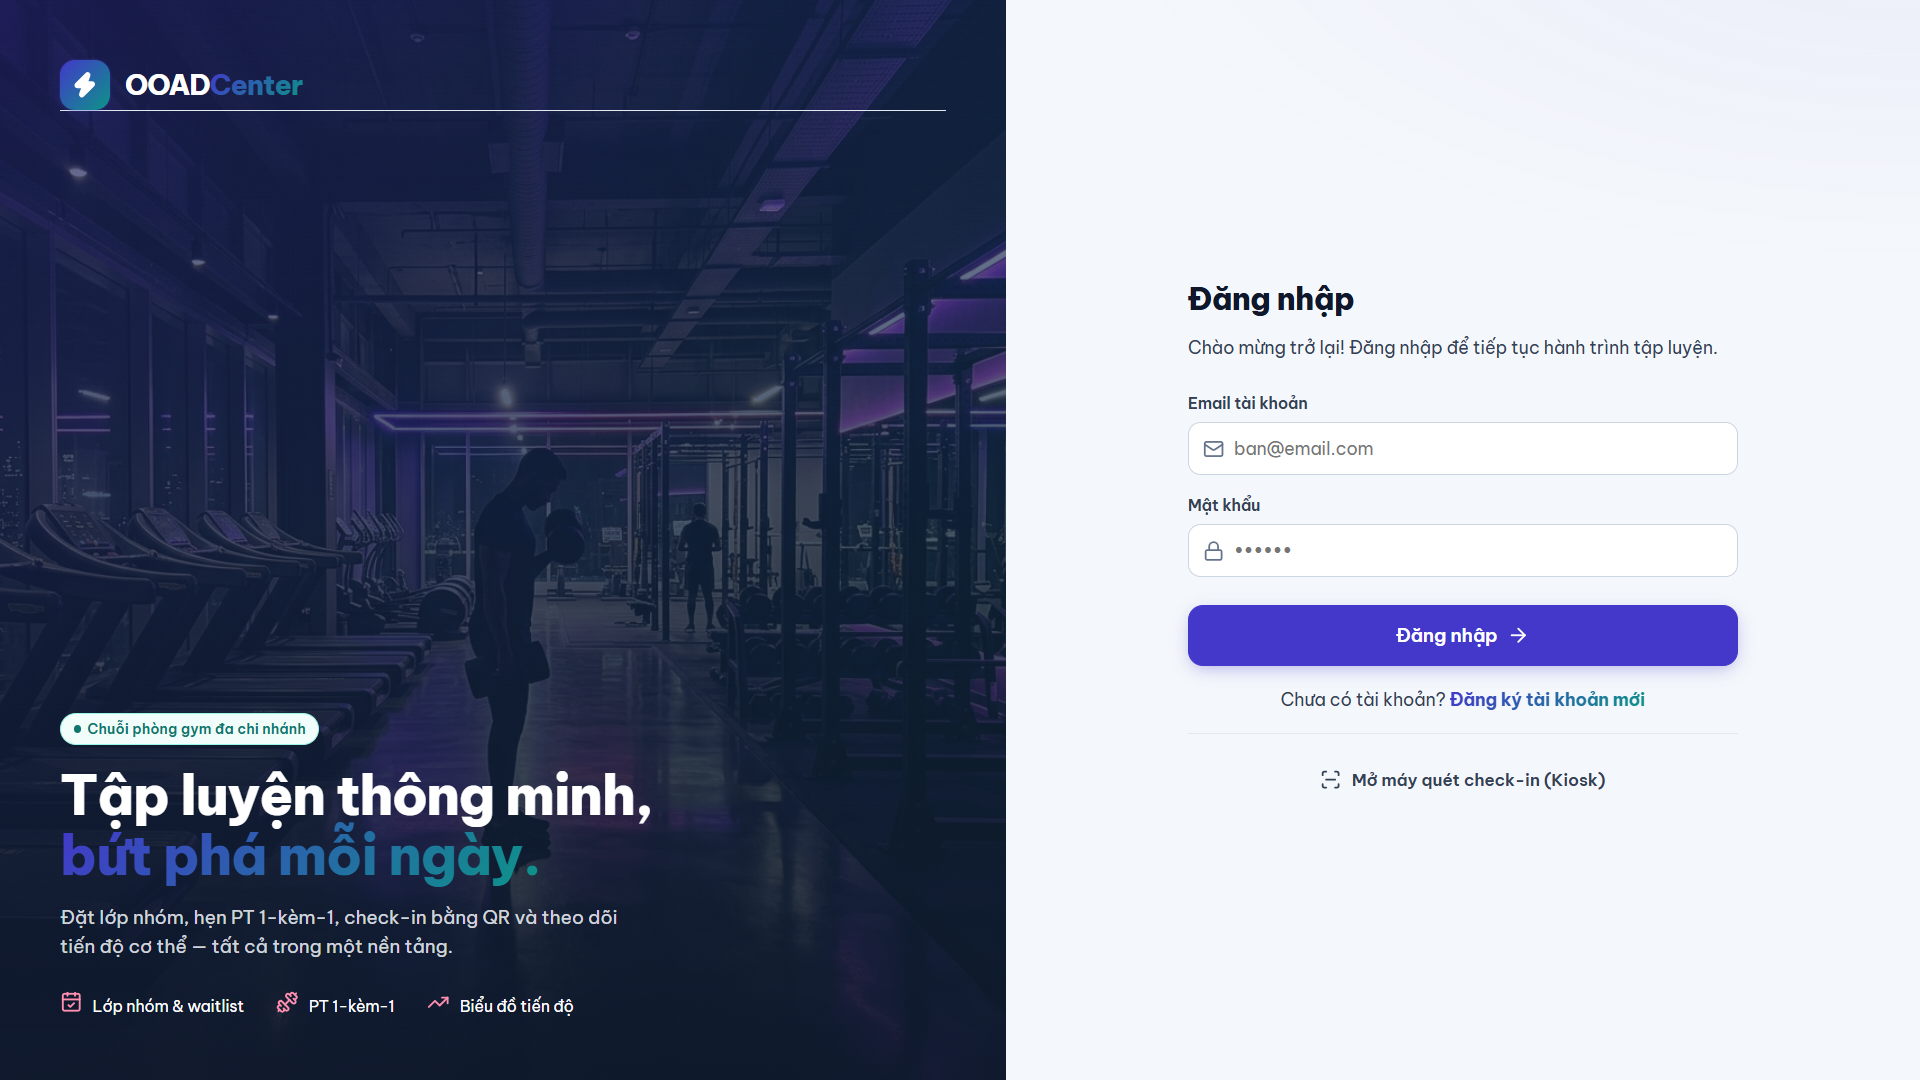
\includegraphics[width=0.92\textwidth]{images/ui_vinh/mh01_login.png}
\caption{Giao diện màn hình Đăng nhập}
\label{fig:mh01_login}
\end{figure}

\par\medskip\noindent\textbf{Danh sách các thành phần giao diện}\par\smallskip
{\footnotesize
\setlength{\tabcolsep}{2.5pt}
\begin{longtable}{|c|L{2.95cm}|L{1.85cm}|L{2.95cm}|L{2.75cm}|L{1.90cm}|L{2.05cm}|}
\hline
\textbf{STT} & \textbf{Tên} & \textbf{Kiểu} & \textbf{Ý nghĩa} & \textbf{Miền giá trị} & \textbf{Giá trị mặc định} & \textbf{Ghi chú} \\
\hline
\endfirsthead
\hline
\textbf{STT} & \textbf{Tên} & \textbf{Kiểu} & \textbf{Ý nghĩa} & \textbf{Miền giá trị} & \textbf{Giá trị mặc định} & \textbf{Ghi chú} \\
\hline
\endhead
\hline
\endfoot
\hline
\caption{Danh sách các thành phần giao diện -- Màn hình Đăng nhập} \\
\endlastfoot
1 & \texttt{Txt\_Email} & Textbox & Nhập địa chỉ email đã đăng ký tài khoản & Chuỗi đúng định dạng email & Rỗng & Bắt buộc nhập \\ \hline
2 & \texttt{Txt\_MatKhau} & Textbox & Nhập mật khẩu bảo mật của tài khoản (che ký tự) & Chuỗi ký tự bất kỳ & Rỗng & Bắt buộc nhập \\ \hline
3 & \texttt{Btn\_DangNhap} & Button & Gửi thông tin xác thực lên hệ thống máy chủ & Kích hoạt / Đang xử lý & \texttt{"Đăng nhập"} & Nút hành động chính \\ \hline
4 & \texttt{Lnk\_DangKy} & Hyperlink & Điều hướng sang màn hình tạo tài khoản mới (\texttt{/register}) & Kích hoạt & \texttt{"Đăng ký"} & Dành cho khách mới \\* \hline
5 & \texttt{Btn\_MoKiosk} & Button & Mở nhanh màn hình Kiosk tự động check-in tại quầy (\texttt{/kiosk}) & Kích hoạt & \texttt{"Mở Kiosk"} & Không cần đăng nhập \\ \hline
\end{longtable}
}

\par\medskip\noindent\textbf{Danh sách các biến cố}\par\smallskip
{\footnotesize
\setlength{\tabcolsep}{4pt}
\begin{longtable}{|c|L{3.5cm}|L{7.8cm}|L{3.5cm}|}
\hline
\textbf{STT} & \textbf{Điều kiện kích hoạt} & \textbf{Xử lý} & \textbf{Ghi chú} \\
\hline
\endfirsthead
\hline
\textbf{STT} & \textbf{Điều kiện kích hoạt} & \textbf{Xử lý} & \textbf{Ghi chú} \\
\hline
\endhead
\hline
\endfoot
\hline
\caption{Danh sách các biến cố -- Màn hình Đăng nhập} \\
\endlastfoot
0 & Khởi động màn hình (\texttt{/login}) & Khởi tạo biểu mẫu trống; kiểm tra phiên đăng nhập hiện có trong trình duyệt, nếu người dùng đã đăng nhập hợp lệ thì tự động chuyển hướng về trang chủ theo vai trò. & Đảm bảo không phải đăng nhập lại khi còn phiên. \\ \hline
1 & Nhấn \texttt{Btn\_DangNhap} khi thiếu trường bắt buộc & Kiểm tra ràng buộc phía giao diện (Boundary); chặn gửi yêu cầu lên máy chủ và hiển thị thông báo yêu cầu nhập đầy đủ Email và Mật khẩu. & Phản hồi tức thì tại trình duyệt. \\ \hline
2 & Nhấn \texttt{Btn\_DangNhap} với thông tin sai & Gửi \texttt{POST /api/auth/login}; máy chủ đối chiếu không khớp và trả về mã lỗi 400; giao diện hiển thị Toast lỗi \textit{``Email hoặc mật khẩu không chính xác''}. & Không tiết lộ trường nào bị sai để bảo mật. \\ \hline
3 & Nhấn \texttt{Btn\_DangNhap} với tài khoản đang bị khóa & Hệ thống kiểm tra trạng thái tài khoản là \texttt{LOCKED}, từ chối cấp phiên làm việc và hiển thị Toast cảnh báo \textit{``Tài khoản đã bị khóa. Vui lòng liên hệ quản trị viên.''}. & Ngăn truy cập trái phép. \\ \hline
4 & Nhấn \texttt{Btn\_DangNhap} với thông tin hợp lệ & Xác thực mật khẩu BCrypt khớp trên máy chủ, sinh JWT token; lưu token phiên làm việc, hiển thị Toast chào mừng và chuyển hướng về Dashboard đúng vai trò. & Hỗ trợ 4 vai trò Member, Trainer, Staff, Admin. \\* \hline
5 & Nhấn \texttt{Lnk\_DangKy} hoặc \texttt{Btn\_MoKiosk} & Điều hướng người dùng sang trang đăng ký tài khoản (\texttt{/register}) hoặc chế độ Kiosk check-in tại quầy (\texttt{/kiosk}). & Không làm thay đổi dữ liệu phiên hiện tại. \\ \hline
\end{longtable}
}

% ==========================================
% 6.2.2 MÀN HÌNH ĐĂNG KÝ HỘI VIÊN
% ==========================================
\subsubsection{Màn hình Đăng ký Hội viên (Khách)}
Màn hình \textbf{Đăng ký Hội viên} (đường dẫn \texttt{/register}, mặc định tab Hội viên) cho phép \textbf{Khách hàng mới} tự tạo tài khoản hội viên cá nhân trên hệ thống \textbf{DFGymCenter}, khai báo thông tin liên hệ, giới tính, ngày sinh và tự động cấp mã thẻ thành viên khởi tạo.

\begin{figure}[H]
\centering
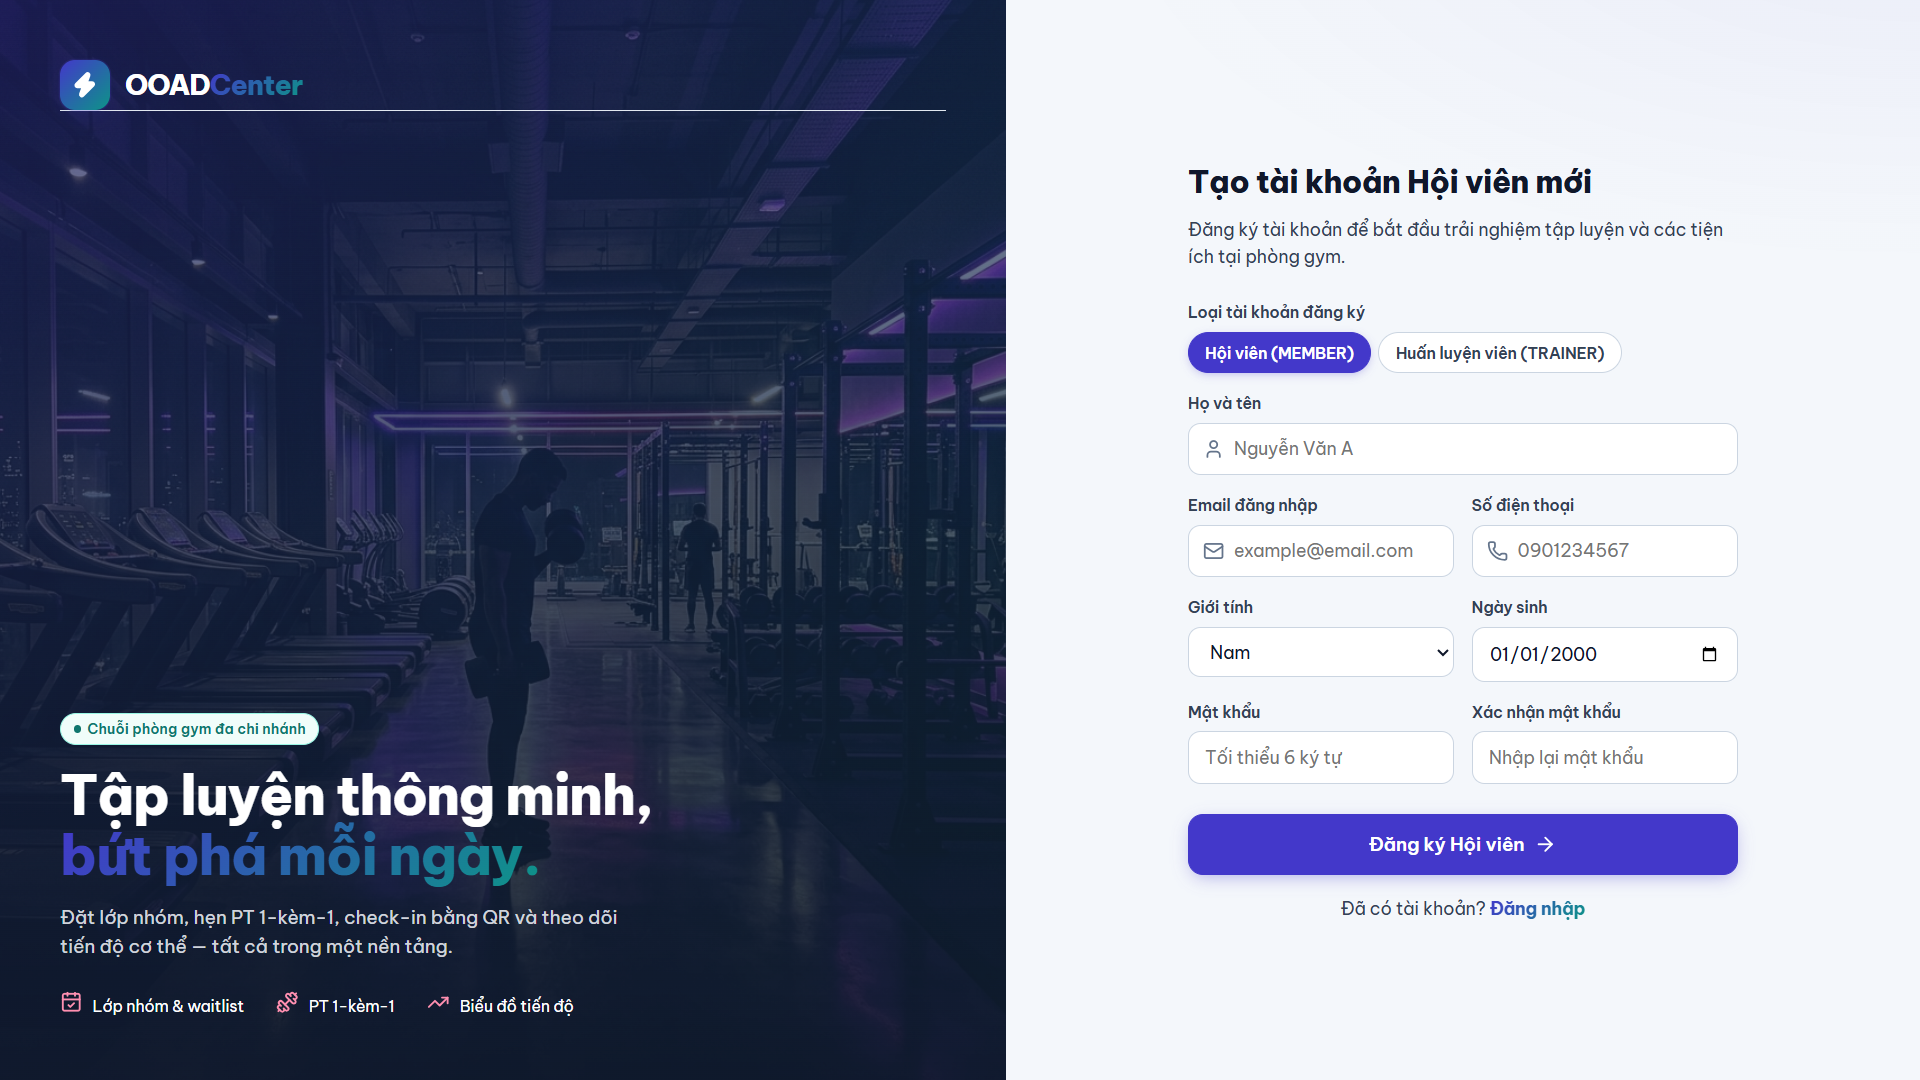
\includegraphics[width=0.92\textwidth]{images/ui_vinh/mh02_register_member.png}
\caption{Giao diện màn hình Đăng ký Hội viên}
\label{fig:mh02_register_member}
\end{figure}

\par\medskip\noindent\textbf{Danh sách các thành phần giao diện}\par\smallskip
{\footnotesize
\setlength{\tabcolsep}{2.5pt}
\begin{longtable}{|c|L{2.95cm}|L{1.85cm}|L{2.95cm}|L{2.75cm}|L{1.90cm}|L{2.05cm}|}
\hline
\textbf{STT} & \textbf{Tên} & \textbf{Kiểu} & \textbf{Ý nghĩa} & \textbf{Miền giá trị} & \textbf{Giá trị mặc định} & \textbf{Ghi chú} \\
\hline
\endfirsthead
\hline
\textbf{STT} & \textbf{Tên} & \textbf{Kiểu} & \textbf{Ý nghĩa} & \textbf{Miền giá trị} & \textbf{Giá trị mặc định} & \textbf{Ghi chú} \\
\hline
\endhead
\hline
\endfoot
\hline
\caption{Danh sách các thành phần giao diện -- Màn hình Đăng ký Hội viên} \\
\endlastfoot
1 & \texttt{Chip\_VaiTroHV} & Chip Button & Chọn loại tài khoản đăng ký là Hội viên & Chọn / Không chọn & Đang chọn (Active) & Mặc định khi mở \texttt{/register} \\ \hline
2 & \texttt{Txt\_HoTen} & Textbox & Nhập họ và tên đầy đủ của hội viên & Chuỗi ký tự không rỗng & Rỗng & Bắt buộc \\ \hline
3 & \texttt{Txt\_EmailDK} & Textbox & Địa chỉ email liên hệ kiêm tên đăng nhập & Chuỗi email duy nhất & Rỗng & Bắt buộc, không trùng \\ \hline
4 & \texttt{Txt\_SoDienThoai} & Textbox & Số điện thoại liên lạc cá nhân & Chuỗi 10 chữ số (bắt đầu bằng 0) & Rỗng & Bắt buộc \\ \hline
5 & \texttt{Cbo\_GioiTinh} & ComboBox & Lựa chọn giới tính hội viên & \{\texttt{"Nam"}, \texttt{"Nữ"}, \texttt{"Khác"}\} & \texttt{"Nam"} & Phục vụ tính chỉ số thể hình \\ \hline
6 & \texttt{Dt\_NgaySinh} & DatePicker & Chọn ngày tháng năm sinh của hội viên & Định dạng \texttt{YYYY-MM-DD} & \texttt{1998-01-01} & Phục vụ theo dõi thể trạng theo độ tuổi \\ \hline
7 & \texttt{Txt\_MatKhauDK} & Textbox & Thiết lập mật khẩu đăng nhập mới (che ký tự) & Chuỗi tối thiểu 6 ký tự & Rỗng & Bắt buộc \\ \hline
8 & \texttt{Txt\_XacNhanMK} & Textbox & Nhập lại mật khẩu để kiểm tra khớp chính xác & Phải khớp \texttt{Txt\_MatKhauDK} & Rỗng & Chặn gửi nếu không khớp \\* \hline
9 & \texttt{Btn\_GuiDangKy} & Button & Gửi biểu mẫu đăng ký tài khoản hội viên mới & Kích hoạt / Đang xử lý & \texttt{"Đăng ký"} & Nút hành động chính \\ \hline
\end{longtable}
}

\par\medskip\noindent\textbf{Danh sách các biến cố}\par\smallskip
{\footnotesize
\setlength{\tabcolsep}{4pt}
\begin{longtable}{|c|L{3.5cm}|L{7.8cm}|L{3.5cm}|}
\hline
\textbf{STT} & \textbf{Điều kiện kích hoạt} & \textbf{Xử lý} & \textbf{Ghi chú} \\
\hline
\endfirsthead
\hline
\textbf{STT} & \textbf{Điều kiện kích hoạt} & \textbf{Xử lý} & \textbf{Ghi chú} \\
\hline
\endhead
\hline
\endfoot
\hline
\caption{Danh sách các biến cố -- Màn hình Đăng ký Hội viên} \\
\endlastfoot
0 & Khởi động màn hình (\texttt{/register}) & Nạp danh sách chi nhánh phục vụ chuyển đổi tab; đặt chip vai trò mặc định là \textit{Hội viên} (\texttt{Chip\_VaiTroHV}) và khởi tạo các trường nhập liệu trống. & Sẵn sàng thu nhận thông tin đăng ký. \\ \hline
1 & Nhấn \texttt{Btn\_GuiDangKy} khi mật khẩu xác nhận không khớp & Kiểm tra đối chiếu giá trị \texttt{Txt\_MatKhauDK} và \texttt{Txt\_XacNhanMK} ngay tại giao diện; báo lỗi \textit{``Mật khẩu xác nhận không khớp''} và giữ nguyên dữ liệu đã nhập. & Ngăn gửi yêu cầu lỗi lên máy chủ. \\ \hline
2 & Nhấn \texttt{Btn\_GuiDangKy} khi Email đã tồn tại & Gửi yêu cầu đăng ký; \texttt{AuthService} kiểm tra trùng lặp trong CSDL và trả về lỗi; hiển thị thông báo \textit{``Email đã được sử dụng bởi tài khoản khác''}. & Bảo đảm tính duy nhất của định danh. \\* \hline
3 & Nhấn \texttt{Btn\_GuiDangKy} với dữ liệu hợp lệ & Tạo bản ghi \texttt{Users} (\texttt{Role = Member}), khởi tạo thẻ hội viên điện tử mặc định trạng thái \texttt{ACTIVE}, cấp token đăng nhập, hiển thị Toast \textit{``Đăng ký thành công!''} và chuyển đến \texttt{/member/profile}. & Tự động đăng nhập ngay sau khi tạo tài khoản. \\ \hline
\end{longtable}
}

% ==========================================
% 6.2.3 MÀN HÌNH ĐĂNG KÝ HUẤN LUYỆN VIÊN
% ==========================================
\subsubsection{Màn hình Đăng ký Huấn luyện viên (Huấn luyện viên)}
Màn hình \textbf{Đăng ký Huấn luyện viên} (đường dẫn \texttt{/register}, chọn vai trò \textit{Huấn luyện viên}) cho phép \textbf{Huấn luyện viên mới} ứng tuyển và khởi tạo tài khoản chuyên môn trên hệ thống, thu thập đầy đủ chi nhánh công tác chính, chuyên môn giảng dạy và số năm kinh nghiệm.

\begin{figure}[H]
\centering
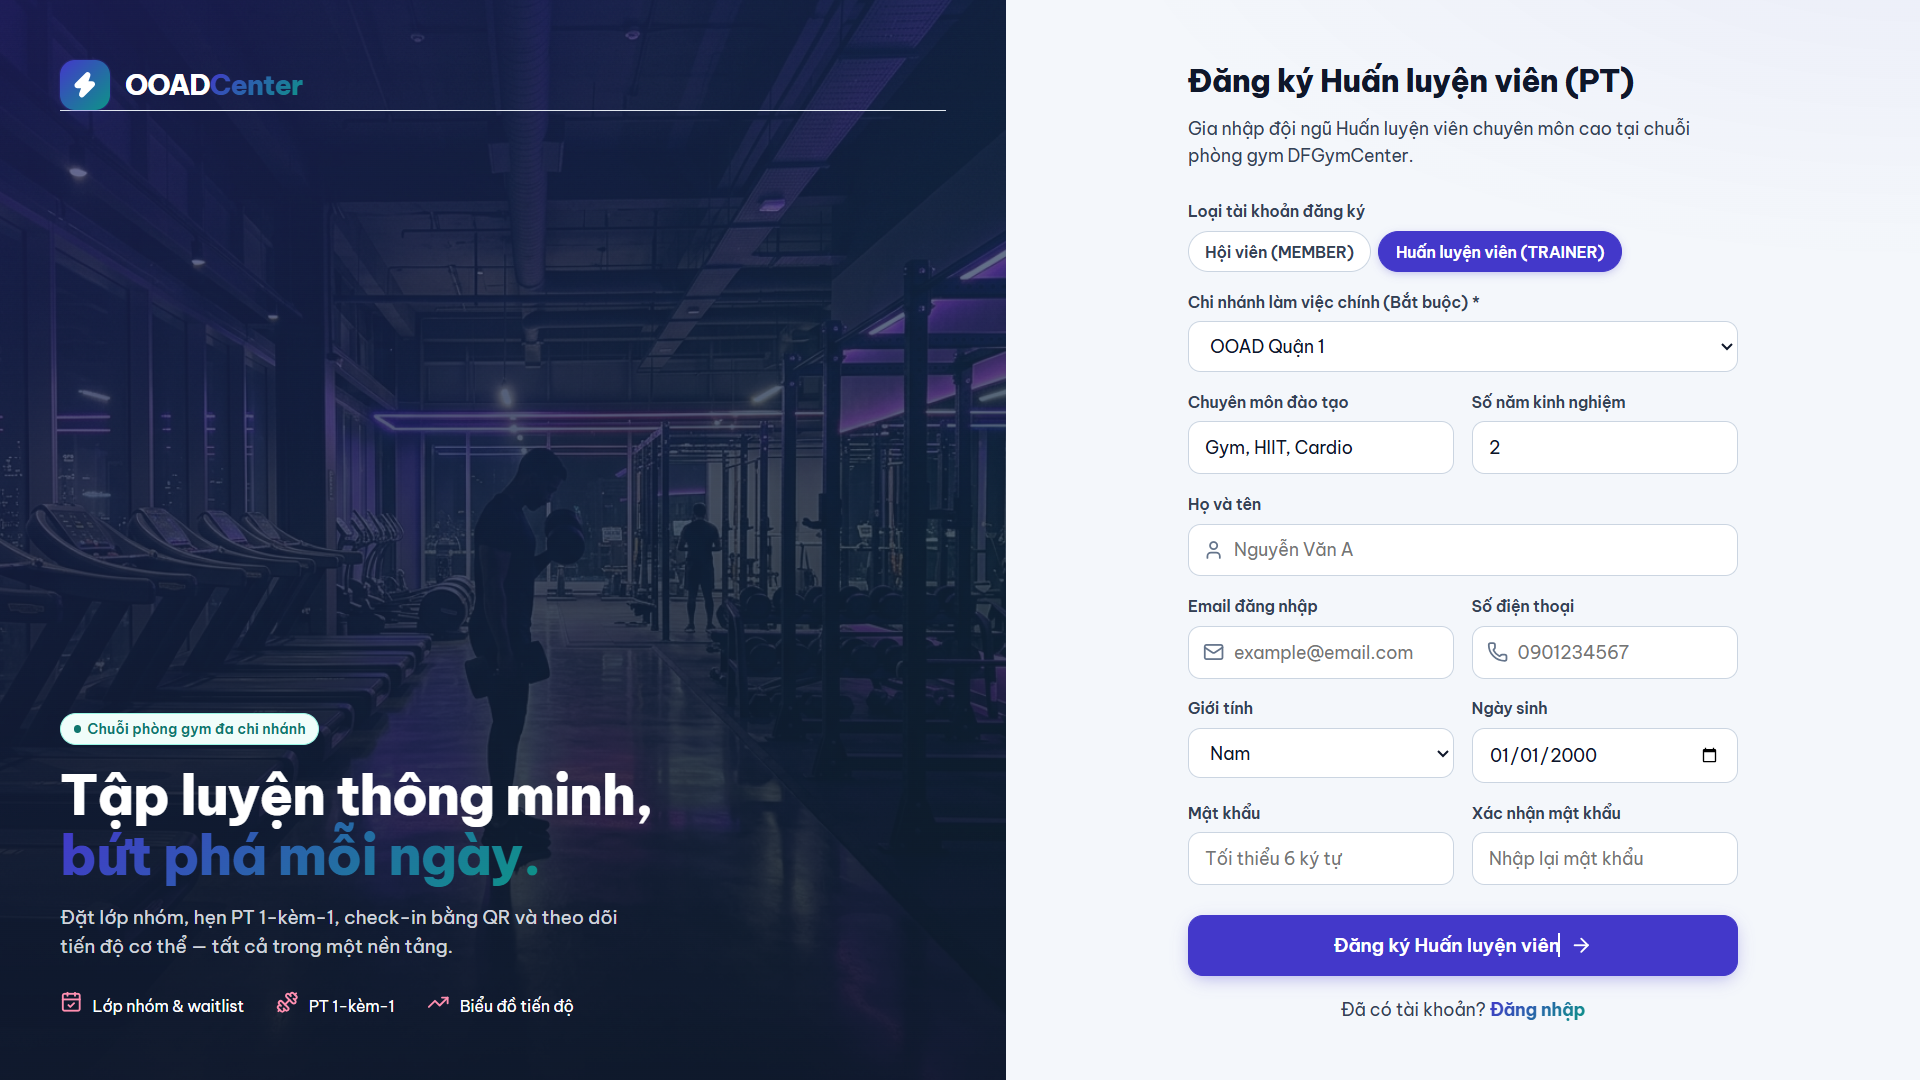
\includegraphics[width=0.92\textwidth]{images/ui_vinh/mh03_register_trainer.png}
\caption{Giao diện màn hình Đăng ký Huấn luyện viên}
\label{fig:mh03_register_trainer}
\end{figure}

\par\medskip\noindent\textbf{Danh sách các thành phần giao diện}\par\smallskip
{\footnotesize
\setlength{\tabcolsep}{2.5pt}
\begin{longtable}{|c|L{2.95cm}|L{1.85cm}|L{2.95cm}|L{2.75cm}|L{1.90cm}|L{2.05cm}|}
\hline
\textbf{STT} & \textbf{Tên} & \textbf{Kiểu} & \textbf{Ý nghĩa} & \textbf{Miền giá trị} & \textbf{Giá trị mặc định} & \textbf{Ghi chú} \\
\hline
\endfirsthead
\hline
\textbf{STT} & \textbf{Tên} & \textbf{Kiểu} & \textbf{Ý nghĩa} & \textbf{Miền giá trị} & \textbf{Giá trị mặc định} & \textbf{Ghi chú} \\
\hline
\endhead
\hline
\endfoot
\hline
\caption{Danh sách các thành phần giao diện -- Màn hình Đăng ký Huấn luyện viên} \\
\endlastfoot
1 & \texttt{Chip\_VaiTroHLV} & Chip Button & Kích hoạt biểu mẫu đăng ký dành riêng cho Huấn luyện viên & Chọn / Không chọn & Đang chọn (Active) & Mở rộng thêm các trường PT \\ \hline
2 & \texttt{Cbo\_ChiNhanhPT} & ComboBox & Chọn chi nhánh làm việc chính của Huấn luyện viên & Danh sách chi nhánh từ \texttt{Branches} & Rỗng (chưa chọn) & Bắt buộc chọn 1 chi nhánh \\ \hline
3 & \texttt{Txt\_ChuyenMonPT} & Textbox & Khai báo các bộ môn huấn luyện chuyên sâu & Chuỗi phân tách dấu phẩy (\texttt{Gym, Yoga, HIIT...}) & Rỗng & Phục vụ lọc PT khi đặt lịch \\ \hline
4 & \texttt{Num\_KinhNghiem} & NumberInput & Nhập số năm kinh nghiệm giảng dạy thể hình & Số nguyên $\ge 0$ & $0$ & Hiển thị trên hồ sơ công khai \\ \hline
5 & \texttt{Grp\_ThongTinChung} & Form Group & Nhóm trường thông tin cá nhân: Họ tên, Email, SĐT, Giới tính, Ngày sinh, Mật khẩu & Giống màn hình Đăng ký Hội viên & Rỗng & Dùng chung quy tắc kiểm tra \\* \hline
6 & \texttt{Btn\_DangKyHLV} & Button & Gửi hồ sơ đăng ký tài khoản Huấn luyện viên lên hệ thống & Kích hoạt / Đang xử lý & \texttt{"Đăng ký"} & Nút hành động chính \\ \hline
\end{longtable}
}

\par\medskip\noindent\textbf{Danh sách các biến cố}\par\smallskip
{\footnotesize
\setlength{\tabcolsep}{4pt}
\begin{longtable}{|c|L{3.5cm}|L{7.8cm}|L{3.5cm}|}
\hline
\textbf{STT} & \textbf{Điều kiện kích hoạt} & \textbf{Xử lý} & \textbf{Ghi chú} \\
\hline
\endfirsthead
\hline
\textbf{STT} & \textbf{Điều kiện kích hoạt} & \textbf{Xử lý} & \textbf{Ghi chú} \\
\hline
\endhead
\hline
\endfoot
\hline
\caption{Danh sách các biến cố -- Màn hình Đăng ký Huấn luyện viên} \\
\endlastfoot
0 & Khởi động màn hình (\texttt{/register}, chọn chip \textit{Huấn luyện viên}) & Tải danh sách chi nhánh đang hoạt động từ API vào \texttt{Cbo\_ChiNhanhPT}; kích hoạt trạng thái \texttt{Chip\_VaiTroHLV} và hiển thị nhóm trường chuyên môn PT. & Cho phép chuyển qua lại với tab Hội viên. \\ \hline
1 & Nhấn chọn \texttt{Chip\_VaiTroHLV} từ tab Hội viên & Giao diện Boundary mở rộng biểu mẫu, bổ sung các ô \texttt{Cbo\_ChiNhanhPT}, \texttt{Txt\_ChuyenMonPT} và \texttt{Num\_KinhNghiem}. & Giữ lại thông tin cá nhân đã nhập. \\ \hline
2 & Nhấn \texttt{Btn\_DangKyHLV} khi chưa chọn chi nhánh & Kiểm tra \texttt{BranchId} bị rỗng; chặn gửi và hiển thị Toast cảnh báo \textit{``Huấn luyện viên bắt buộc phải chọn Chi nhánh!''}. & Đảm bảo HLV luôn gắn với ít nhất 1 cơ sở. \\* \hline
3 & Nhấn \texttt{Btn\_DangKyHLV} với dữ liệu hợp lệ & Tạo tài khoản \texttt{Users} (\texttt{Role = Trainer}) và hồ sơ chuyên môn \texttt{Trainers}; hiển thị Toast \textit{``Đăng ký thành công!''} và chuyển hướng về \texttt{/trainer/profile}. & Sẵn sàng bổ sung chứng chỉ và giới thiệu. \\ \hline
\end{longtable}
}

% ==========================================
% 6.2.4 MÀN HÌNH HỒ SƠ HỘI VIÊN
% ==========================================
\subsubsection{Màn hình Hồ sơ Hội viên (Hội viên)}
Màn hình \textbf{Hồ sơ Hội viên} (đường dẫn \texttt{/member/profile}) cho phép \textbf{Hội viên} cập nhật thông tin cá nhân, thay đổi mật khẩu bảo mật và xuất trình thẻ hội viên điện tử kèm mã QR động hoặc báo mất thẻ khẩn cấp ngay tại trang hồ sơ.

\begin{figure}[H]
\centering
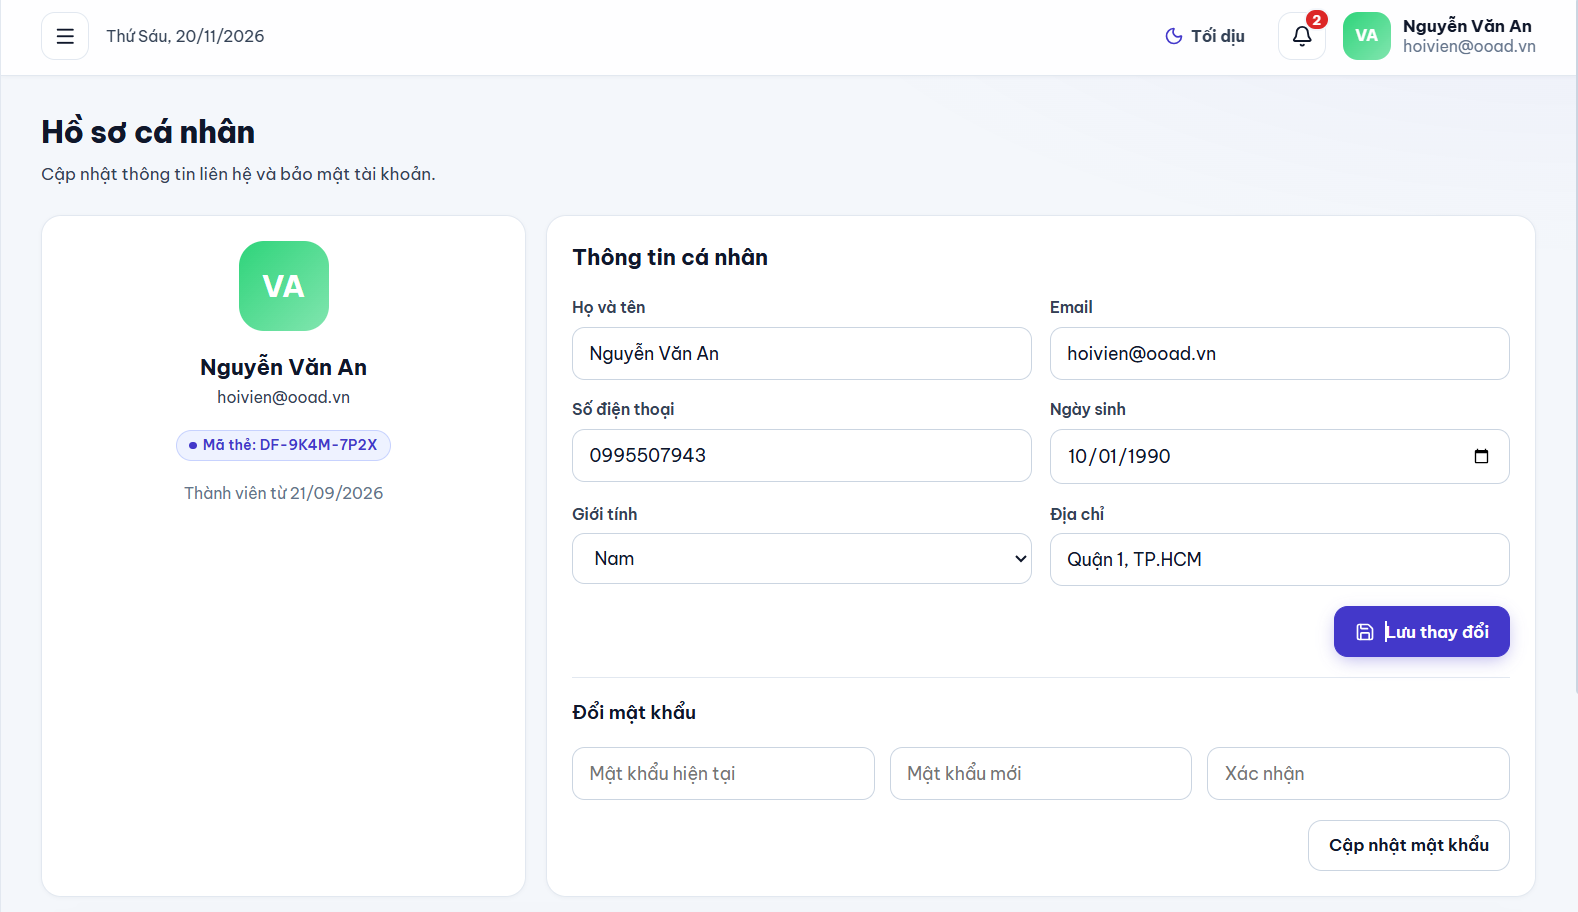
\includegraphics[width=0.92\textwidth]{images/ui_vinh/mh04_profile_member.png}
\caption{Giao diện màn hình Hồ sơ Hội viên}
\label{fig:mh04_profile_member}
\end{figure}

\par\medskip\noindent\textbf{Danh sách các thành phần giao diện}\par\smallskip
{\footnotesize
\setlength{\tabcolsep}{2.5pt}
\begin{longtable}{|c|L{2.95cm}|L{1.85cm}|L{2.95cm}|L{2.75cm}|L{1.90cm}|L{2.05cm}|}
\hline
\textbf{STT} & \textbf{Tên} & \textbf{Kiểu} & \textbf{Ý nghĩa} & \textbf{Miền giá trị} & \textbf{Giá trị mặc định} & \textbf{Ghi chú} \\
\hline
\endfirsthead
\hline
\textbf{STT} & \textbf{Tên} & \textbf{Kiểu} & \textbf{Ý nghĩa} & \textbf{Miền giá trị} & \textbf{Giá trị mặc định} & \textbf{Ghi chú} \\
\hline
\endhead
\hline
\endfoot
\hline
\caption{Danh sách các thành phần giao diện -- Màn hình Hồ sơ Hội viên} \\
\endlastfoot
1 & \texttt{Card\_TomTatHV} & Card Panel & Hiển thị Avatar, Họ tên, Email, Mã thẻ từ và ngày tham gia hệ thống & Thông tin tổng hợp từ \texttt{Users} và \texttt{Member\_Cards} & Theo người dùng đăng nhập & Chỉ đọc \\ \hline
2 & \texttt{Txt\_HoTenHV} & Textbox & Chỉnh sửa họ và tên hiển thị của hội viên & Chuỗi ký tự không rỗng & Giá trị hiện tại & Bắt buộc \\ \hline
3 & \texttt{Txt\_SoDienThoaiHV} & Textbox & Cập nhật số điện thoại liên lạc & Chuỗi 10 chữ số & Giá trị hiện tại & Bắt buộc \\ \hline
4 & \texttt{Btn\_LuuHoSoHV} & Button & Lưu các thay đổi thông tin cá nhân vào CSDL & Kích hoạt & \texttt{"Lưu thay đổi"} & Nút hành động chính \\ \hline
5 & \texttt{Grp\_DoiMatKhau} & Form Group & Nhóm 3 ô nhập Mật khẩu hiện tại, Mật khẩu mới, Xác nhận và nút \texttt{Cập nhật mật khẩu} & Tối thiểu 6 ký tự & Rỗng & Kiểm tra khớp mật khẩu mới \\* \hline
6 & \texttt{Wgt\_TheHoiVien} & Component & Thành phần \texttt{MemberCardWidget} hiển thị thẻ điện tử, mã QR động check-in và nút báo mất thẻ & Trạng thái \texttt{ACTIVE} / \texttt{LOCKED} / \texttt{LOST} & Theo thẻ hiện hành & Dùng chung với \texttt{/member/card} \\ \hline
\end{longtable}
}

\par\medskip\noindent\textbf{Danh sách các biến cố}\par\smallskip
{\footnotesize
\setlength{\tabcolsep}{4pt}
\begin{longtable}{|c|L{3.5cm}|L{7.8cm}|L{3.5cm}|}
\hline
\textbf{STT} & \textbf{Điều kiện kích hoạt} & \textbf{Xử lý} & \textbf{Ghi chú} \\
\hline
\endfirsthead
\hline
\textbf{STT} & \textbf{Điều kiện kích hoạt} & \textbf{Xử lý} & \textbf{Ghi chú} \\
\hline
\endhead
\hline
\endfoot
\hline
\caption{Danh sách các biến cố -- Màn hình Hồ sơ Hội viên} \\
\endlastfoot
0 & Khởi động màn hình (\texttt{/member/profile}) & Nạp thông tin cá nhân từ phiên người dùng hiện tại vào biểu mẫu; tải dữ liệu thẻ hội viên và lịch sử cấp thẻ vào \texttt{Wgt\_TheHoiVien}. & Trường Email bị khóa chỉ đọc để giữ định danh. \\ \hline
1 & Nhấn \texttt{Btn\_LuuHoSoHV} khi Họ tên bị rỗng & Kiểm tra hợp lệ tại Boundary UI; chặn gửi và hiển thị thông báo lỗi \textit{``Họ tên không được để trống''}. & Giữ nguyên trạng thái biểu mẫu để sửa. \\ \hline
2 & Nhấn \texttt{Btn\_LuuHoSoHV} với dữ liệu hợp lệ & Gửi \texttt{PUT /api/users/me} cập nhật thực thể \texttt{Users} vào CSDL; hiển thị Toast \textit{``Đã lưu hồ sơ thành công''}. & Cập nhật ngay tên hiển thị trên thanh tiêu đề. \\ \hline
3 & Thực hiện đổi mật khẩu khi nhập sai mật khẩu cũ & Đối chiếu mật khẩu hiện tại không khớp; trả lỗi \textit{``Mật khẩu hiện tại không đúng''} và không cập nhật. & Bảo vệ an toàn tài khoản. \\ \hline
4 & Đổi mật khẩu khi dữ liệu khớp và đạt chuẩn ($\ge 6$ ký tự) & Băm (hash) mật khẩu mới, lưu vào CSDL; hiển thị Toast \textit{``Đổi mật khẩu thành công''} và làm trống 3 ô trong \texttt{Grp\_DoiMatKhau}. & Duy trì phiên làm việc hiện tại. \\* \hline
5 & Nhấn \textit{``Báo mất thẻ''} trên \texttt{Wgt\_TheHoiVien} & Xác nhận và chuyển trạng thái thẻ từ \texttt{ACTIVE} sang \texttt{LOST}; hiển thị cảnh báo thẻ đã bị khóa vĩnh viễn và hướng dẫn liên hệ lễ tân cấp thẻ mới. & Vô hiệu hóa quét QR của thẻ cũ tức thời. \\ \hline
\end{longtable}
}

% ==========================================
% 6.2.5 MÀN HÌNH HỒ SƠ HUẤN LUYỆN VIÊN
% ==========================================
\subsubsection{Màn hình Hồ sơ Huấn luyện viên (Huấn luyện viên)}
Màn hình \textbf{Hồ sơ Huấn luyện viên} (đường dẫn \texttt{/trainer/profile}) cho phép \textbf{Huấn luyện viên (PT)} quản lý và công khai hồ sơ năng lực chuyên môn, bao gồm chuyên môn giảng dạy, thâm niên, chứng chỉ quốc tế, lời giới thiệu và các chi nhánh nhận lịch dạy 1-kèm-1.

\begin{figure}[H]
\centering
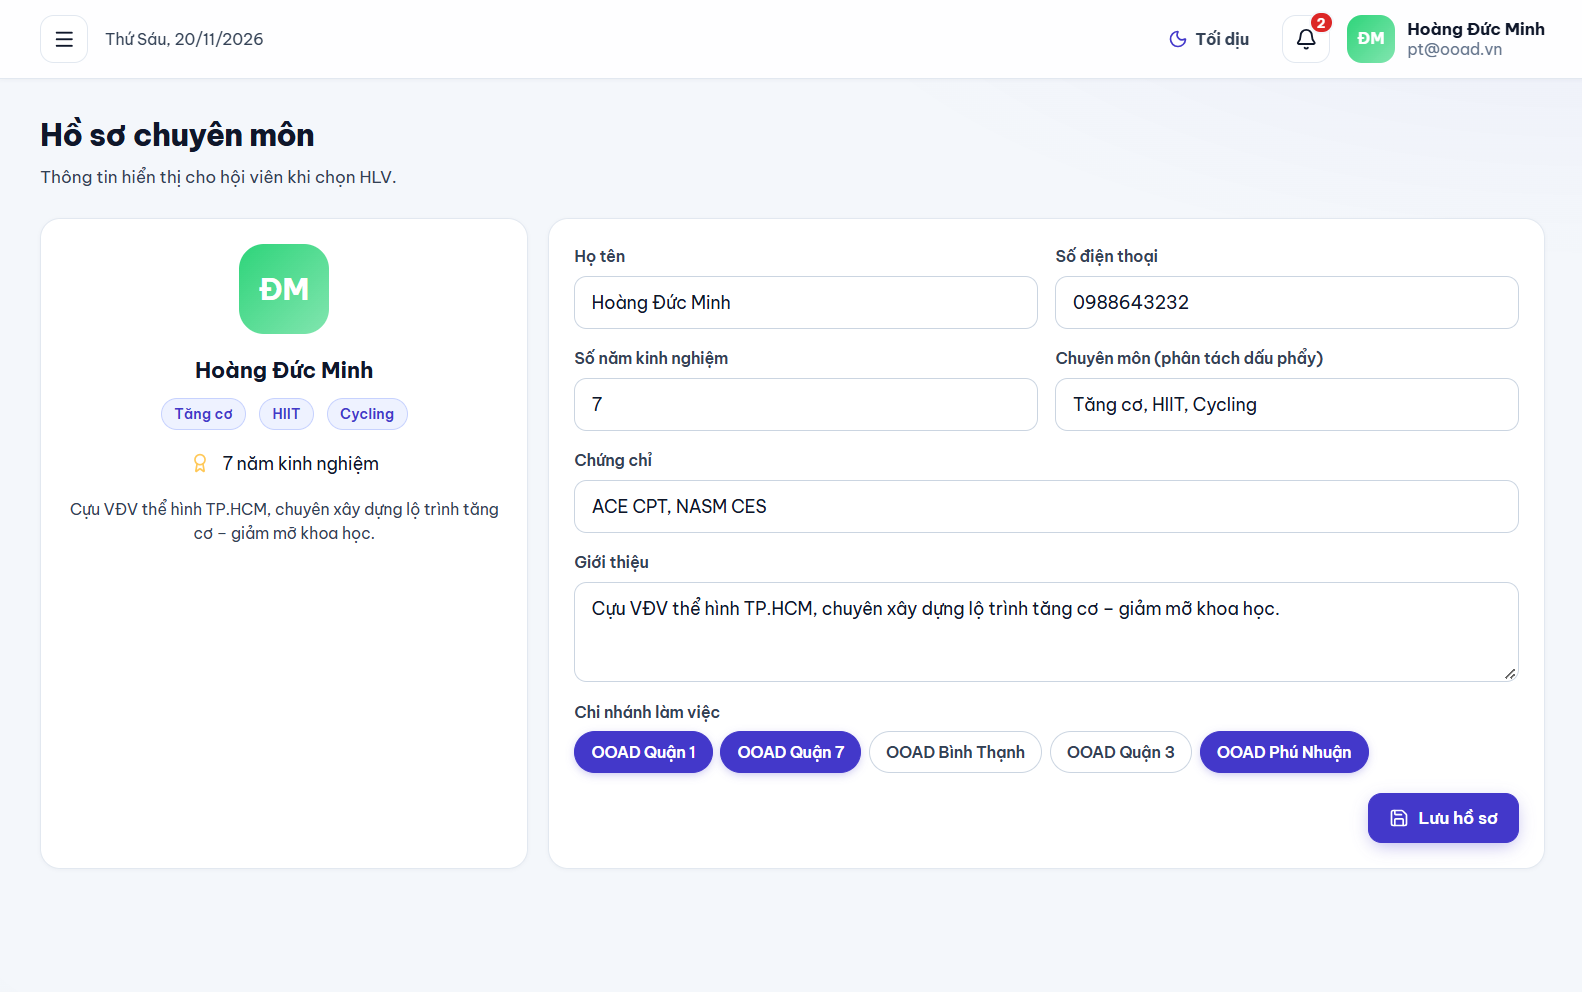
\includegraphics[width=0.92\textwidth]{images/ui_vinh/mh05_profile_trainer.png}
\caption{Giao diện màn hình Hồ sơ Huấn luyện viên}
\label{fig:mh05_profile_trainer}
\end{figure}

\par\medskip\noindent\textbf{Danh sách các thành phần giao diện}\par\smallskip
{\footnotesize
\setlength{\tabcolsep}{2.5pt}
\begin{longtable}{|c|L{2.95cm}|L{1.85cm}|L{2.95cm}|L{2.75cm}|L{1.90cm}|L{2.05cm}|}
\hline
\textbf{STT} & \textbf{Tên} & \textbf{Kiểu} & \textbf{Ý nghĩa} & \textbf{Miền giá trị} & \textbf{Giá trị mặc định} & \textbf{Ghi chú} \\
\hline
\endfirsthead
\hline
\textbf{STT} & \textbf{Tên} & \textbf{Kiểu} & \textbf{Ý nghĩa} & \textbf{Miền giá trị} & \textbf{Giá trị mặc định} & \textbf{Ghi chú} \\
\hline
\endhead
\hline
\endfoot
\hline
\caption{Danh sách các thành phần giao diện -- Màn hình Hồ sơ Huấn luyện viên} \\
\endlastfoot
1 & \texttt{Card\_NangLucPT} & Card Panel & Khối xem trước hồ sơ công khai: badge chuyên môn, điểm sao đánh giá và thâm niên & Dữ liệu từ \texttt{Trainers} và \texttt{Reviews} & Theo hồ sơ HLV hiện tại & Chỉ đọc (Preview) \\ \hline
2 & \texttt{Txt\_HoTenPT} & Textbox & Họ và tên hiển thị công khai của Huấn luyện viên & Chuỗi ký tự không rỗng & Giá trị hiện tại & Bắt buộc \\ \hline
3 & \texttt{Txt\_SoDienThoaiPT} & Textbox & Số điện thoại liên hệ của Huấn luyện viên & Chuỗi 10 chữ số & Giá trị hiện tại & Bắt buộc \\ \hline
4 & \texttt{Num\_KinhNghiemPT} & NumberInput & Số năm kinh nghiệm giảng dạy thể hình & Số nguyên $\ge 0$ & Giá trị hiện tại & Hiển thị trên trang đặt PT \\ \hline
5 & \texttt{Txt\_ChuyenMon} & Textbox & Danh mục chuyên môn giảng dạy (phân tách bởi dấu phẩy) & Chuỗi ký tự (\texttt{Yoga, Gym, HIIT...}) & Giá trị hiện tại & Tách thành các nhãn badge \\ \hline
6 & \texttt{Txt\_ChungChi} & Textbox & Khai báo các chứng chỉ chuyên ngành (ACE, NASM, ISSA...) & Chuỗi ký tự & Giá trị hiện tại & Hiển thị cho hội viên tham khảo \\ \hline
7 & \texttt{Txt\_GioiThieuBio} & TextArea & Đoạn văn mô tả phong cách huấn luyện và thành tích cá nhân & Văn bản nhiều dòng & Đoạn bio hiện tại & Tùy chọn nhập \\ \hline
8 & \texttt{Chip\_ChiNhanhPT} & Chip Button & Nhóm nút bật/tắt chọn các chi nhánh HLV có thể nhận dạy & Chọn $\ge 1$ chi nhánh từ \texttt{Branches} & Các chi nhánh đã gán & Bắt buộc chọn ít nhất 1 \\* \hline
9 & \texttt{Btn\_LuuHoSoPT} & Button & Lưu cập nhật hồ sơ chuyên môn HLV vào hệ thống & Kích hoạt & \texttt{"Lưu hồ sơ"} & Nút hành động chính \\ \hline
\end{longtable}
}

\par\medskip\noindent\textbf{Danh sách các biến cố}\par\smallskip
{\footnotesize
\setlength{\tabcolsep}{4pt}
\begin{longtable}{|c|L{3.5cm}|L{7.8cm}|L{3.5cm}|}
\hline
\textbf{STT} & \textbf{Điều kiện kích hoạt} & \textbf{Xử lý} & \textbf{Ghi chú} \\
\hline
\endfirsthead
\hline
\textbf{STT} & \textbf{Điều kiện kích hoạt} & \textbf{Xử lý} & \textbf{Ghi chú} \\
\hline
\endhead
\hline
\endfoot
\hline
\caption{Danh sách các biến cố -- Màn hình Hồ sơ Huấn luyện viên} \\
\endlastfoot
0 & Khởi động màn hình (\texttt{/trainer/profile}) & Gọi API \texttt{GET /api/trainers/me} nạp họ tên, số điện thoại, thâm niên, chuyên môn, chứng chỉ, lời giới thiệu và danh sách chi nhánh đang nhận dạy lên biểu mẫu và thẻ xem trước \texttt{Card\_NangLucPT}. & Cập nhật xem trước tức thời khi sửa. \\ \hline
1 & Nhấn chọn hoặc bỏ chọn một chip trên \texttt{Chip\_ChiNhanhPT} & Thêm hoặc xóa mã chi nhánh (\texttt{BranchId}) khỏi mảng chi nhánh làm việc của HLV và đổi trạng thái màu sắc của chip tương ứng. & Hỗ trợ HLV dạy liên chi nhánh. \\ \hline
2 & Nhấn \texttt{Btn\_LuuHoSoPT} khi bỏ chọn toàn bộ chi nhánh & Kiểm tra danh sách chi nhánh rỗng; chặn lưu và hiển thị thông báo lỗi \textit{``Chọn ít nhất một chi nhánh làm việc''}. & Tránh HLV không xuất hiện trên bộ lọc đặt lịch. \\* \hline
3 & Nhấn \texttt{Btn\_LuuHoSoPT} với dữ liệu hợp lệ & Kiểm tra họ tên không rỗng, số điện thoại hợp lệ, số năm kinh nghiệm $\ge 0$ và chọn ít nhất 1 chi nhánh; gửi \texttt{PUT /api/trainers/me} cập nhật thực thể \texttt{Users} và \texttt{Trainers} vào CSDL; hiển thị Toast \textit{``Đã cập nhật hồ sơ chuyên môn''} và đồng bộ dữ liệu lên trang tra cứu PT của hội viên. & Thay đổi áp dụng ngay lập tức. \\ \hline
\end{longtable}
}

% ==========================================
% 6.2.6 MÀN HÌNH HỒ SƠ NHÂN VIÊN LỄ TÂN
% ==========================================
\subsubsection{Màn hình Hồ sơ Nhân viên Lễ tân (Nhân viên Lễ tân)}
Màn hình \textbf{Hồ sơ Nhân viên Lễ tân} (đường dẫn \texttt{/account}) cho phép \textbf{Nhân viên Lễ tân} xem thông tin định danh công tác, chi nhánh được phân công trực và cập nhật thông tin liên hệ hoặc đổi mật khẩu bảo mật ca trực.

\begin{figure}[H]
\centering
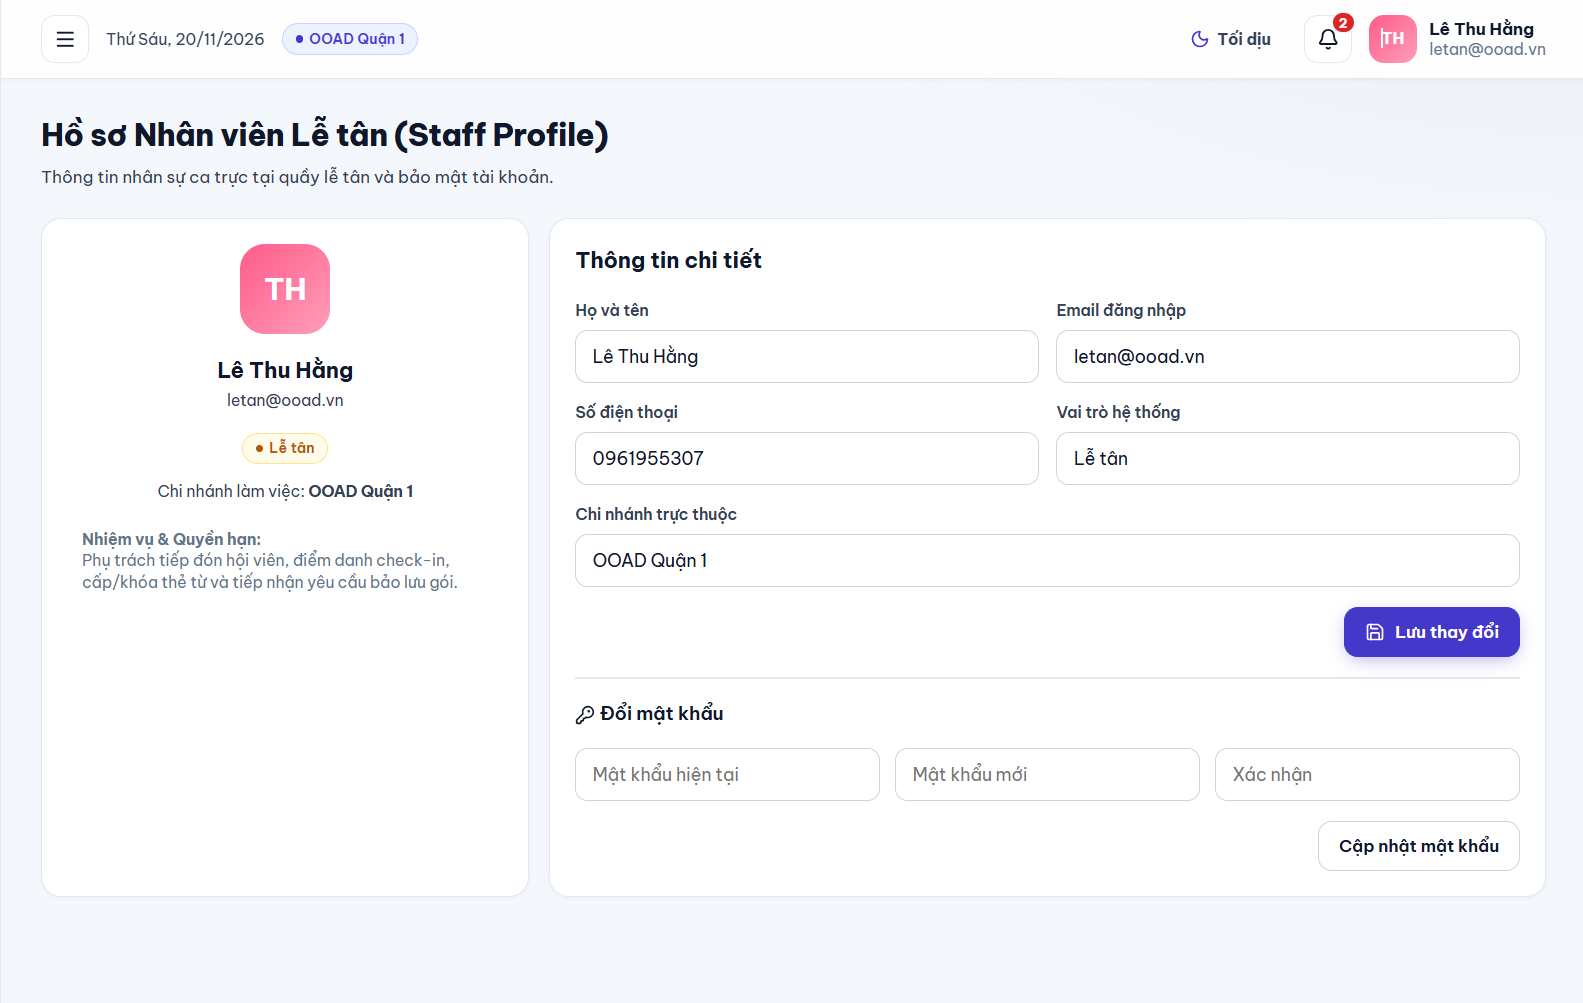
\includegraphics[width=0.92\textwidth]{images/ui_vinh/mh06_profile_staff.png}
\caption{Giao diện màn hình Hồ sơ Nhân viên Lễ tân}
\label{fig:mh06_profile_staff}
\end{figure}

\par\medskip\noindent\textbf{Danh sách các thành phần giao diện}\par\smallskip
{\footnotesize
\setlength{\tabcolsep}{2.5pt}
\begin{longtable}{|c|L{2.95cm}|L{1.85cm}|L{2.95cm}|L{2.75cm}|L{1.90cm}|L{2.05cm}|}
\hline
\textbf{STT} & \textbf{Tên} & \textbf{Kiểu} & \textbf{Ý nghĩa} & \textbf{Miền giá trị} & \textbf{Giá trị mặc định} & \textbf{Ghi chú} \\
\hline
\endfirsthead
\hline
\textbf{STT} & \textbf{Tên} & \textbf{Kiểu} & \textbf{Ý nghĩa} & \textbf{Miền giá trị} & \textbf{Giá trị mặc định} & \textbf{Ghi chú} \\
\hline
\endhead
\hline
\endfoot
\hline
\caption{Danh sách các thành phần giao diện -- Màn hình Hồ sơ Nhân viên Lễ tân} \\
\endlastfoot
1 & \texttt{Card\_NhanSuLT} & Card Panel & Hiển thị Avatar, chức vụ \textit{``Lễ tân''}, chi nhánh công tác và mô tả nhiệm vụ ca trực & Thông tin từ \texttt{Users} và \texttt{Staff} & Theo tài khoản đăng nhập & Chỉ đọc \\ \hline
2 & \texttt{Txt\_HoTenLT} & Textbox & Chỉnh sửa họ và tên hiển thị của nhân viên lễ tân & Chuỗi ký tự không rỗng & Giá trị hiện tại & Bắt buộc \\ \hline
3 & \texttt{Txt\_EmailLT} & Textbox & Email đăng nhập nội bộ được cấp phát & Chuỗi email & Email nhân viên & Chỉ đọc (Vô hiệu hóa sửa) \\ \hline
4 & \texttt{Txt\_SoDienThoaiLT} & Textbox & Cập nhật số điện thoại liên lạc nội bộ & Chuỗi 10 chữ số & Giá trị hiện tại & Bắt buộc \\ \hline
5 & \texttt{Txt\_ChiNhanhLT} & Textbox & Chi nhánh phòng tập mà nhân viên phụ trách ca trực & Tên chi nhánh từ \texttt{Branches} & Chi nhánh được gán & Chỉ đọc (Do Admin gán) \\* \hline
6 & \texttt{Grp\_DoiMKCaTruc} & Form Group & Biểu mẫu nhập mật khẩu cũ/mới để đổi mật khẩu định kỳ bảo vệ quầy giao dịch & Tối thiểu 6 ký tự & Rỗng & Có kiểm tra mật khẩu cũ \\ \hline
\end{longtable}
}

\par\medskip\noindent\textbf{Danh sách các biến cố}\par\smallskip
{\footnotesize
\setlength{\tabcolsep}{4pt}
\begin{longtable}{|c|L{3.5cm}|L{7.8cm}|L{3.5cm}|}
\hline
\textbf{STT} & \textbf{Điều kiện kích hoạt} & \textbf{Xử lý} & \textbf{Ghi chú} \\
\hline
\endfirsthead
\hline
\textbf{STT} & \textbf{Điều kiện kích hoạt} & \textbf{Xử lý} & \textbf{Ghi chú} \\
\hline
\endhead
\hline
\endfoot
\hline
\caption{Danh sách các biến cố -- Màn hình Hồ sơ Nhân viên Lễ tân} \\
\endlastfoot
0 & Khởi động màn hình (\texttt{/account}) & Nạp thông tin nhân viên lễ tân, tên chi nhánh phụ trách từ CSDL lên các thẻ và biểu mẫu; khóa các trường định danh chỉ đọc (\texttt{Txt\_EmailLT}, \texttt{Txt\_ChiNhanhLT}). & Đảm bảo nhân viên không tự đổi chi nhánh. \\ \hline
1 & Nhấn lưu cập nhật thông tin cá nhân & Kiểm tra Họ tên và SĐT hợp lệ; gửi \texttt{PUT /api/users/me} để lưu thông tin nhân viên và hiển thị thông báo cập nhật thành công. & Đồng bộ tên lễ tân trên nhật ký xử lý. \\ \hline
2 & Đổi mật khẩu khi nhập sai mật khẩu hiện tại & Hệ thống đối chiếu xác thực mật khẩu cũ thất bại; hiển thị thông báo lỗi \textit{``Mật khẩu hiện tại không đúng''}. & Giữ nguyên mật khẩu cũ. \\* \hline
3 & Đổi mật khẩu thành công & Mã hóa (hash) và lưu mật khẩu mới vào CSDL; hiển thị Toast \textit{``Đổi mật khẩu thành công''} và ghi nhận nhật ký bảo mật. & Bảo vệ an toàn tài khoản quầy trực. \\ \hline
\end{longtable}
}

% ==========================================
% 6.2.7 MÀN HÌNH HỒ SƠ QUẢN TRỊ VIÊN
% ==========================================
\subsubsection{Màn hình Hồ sơ Quản trị viên (Quản trị viên)}
Màn hình \textbf{Hồ sơ Quản trị viên} (đường dẫn \texttt{/account}) cho phép \textbf{Quản trị viên (Admin)} xem định danh quản trị toàn hệ thống, cập nhật thông tin liên hệ và thực hiện đổi mật khẩu bảo vệ tài khoản quản trị cao nhất.

\begin{figure}[H]
\centering
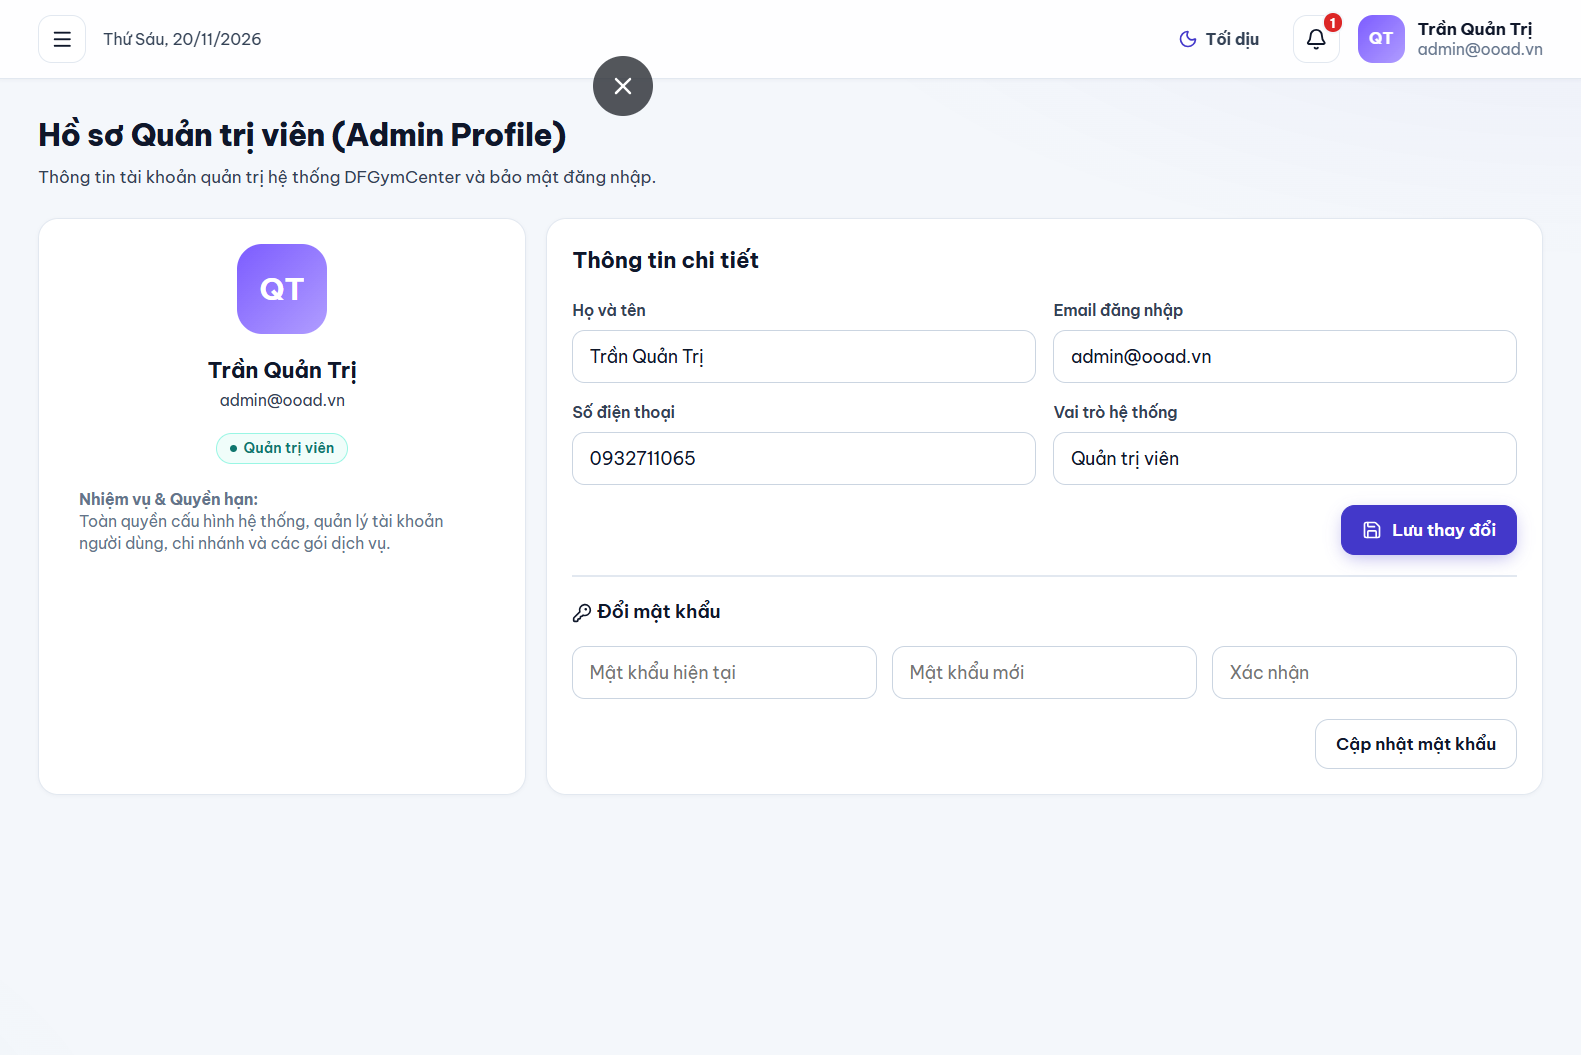
\includegraphics[width=0.92\textwidth]{images/ui_vinh/mh07_profile_admin.png}
\caption{Giao diện màn hình Hồ sơ Quản trị viên}
\label{fig:mh07_profile_admin}
\end{figure}

\par\medskip\noindent\textbf{Danh sách các thành phần giao diện}\par\smallskip
{\footnotesize
\setlength{\tabcolsep}{2.5pt}
\begin{longtable}{|c|L{2.95cm}|L{1.85cm}|L{2.95cm}|L{2.75cm}|L{1.90cm}|L{2.05cm}|}
\hline
\textbf{STT} & \textbf{Tên} & \textbf{Kiểu} & \textbf{Ý nghĩa} & \textbf{Miền giá trị} & \textbf{Giá trị mặc định} & \textbf{Ghi chú} \\
\hline
\endfirsthead
\hline
\textbf{STT} & \textbf{Tên} & \textbf{Kiểu} & \textbf{Ý nghĩa} & \textbf{Miền giá trị} & \textbf{Giá trị mặc định} & \textbf{Ghi chú} \\
\hline
\endhead
\hline
\endfoot
\hline
\caption{Danh sách các thành phần giao diện -- Màn hình Hồ sơ Quản trị viên} \\
\endlastfoot
1 & \texttt{Card\_QuanTriVien} & Card Panel & Hiển thị badge \textit{``Quản trị viên''} và thông tin thẩm quyền toàn chuỗi DFGymCenter & Thông tin tài khoản Admin & Theo tài khoản đăng nhập & Chỉ đọc \\ \hline
2 & \texttt{Txt\_HoTenAdmin} & Textbox & Nhập hoặc chỉnh sửa họ tên đầy đủ của quản trị viên & Chuỗi ký tự không rỗng & Giá trị hiện tại & Bắt buộc \\ \hline
3 & \texttt{Txt\_EmailAdmin} & Textbox & Địa chỉ email sở hữu quyền quản trị hệ thống & Chuỗi email & Email quản trị & Chỉ đọc \\ \hline
4 & \texttt{Txt\_VaiTroAdmin} & Textbox & Hiển thị vai trò thẩm quyền trên hệ thống & Cố định \texttt{"Quản trị viên (Admin)"} & \texttt{"Quản trị viên"} & Chỉ đọc \\* \hline
5 & \texttt{Grp\_DoiMKAdmin} & Form Group & Nhóm ô nhập mật khẩu cũ, mật khẩu mới và xác nhận để bảo vệ tài khoản root & Tối thiểu 6 ký tự & Rỗng & Áp dụng quy chuẩn bảo mật cao \\ \hline
\end{longtable}
}

\par\medskip\noindent\textbf{Danh sách các biến cố}\par\smallskip
{\footnotesize
\setlength{\tabcolsep}{4pt}
\begin{longtable}{|c|L{3.5cm}|L{7.8cm}|L{3.5cm}|}
\hline
\textbf{STT} & \textbf{Điều kiện kích hoạt} & \textbf{Xử lý} & \textbf{Ghi chú} \\
\hline
\endfirsthead
\hline
\textbf{STT} & \textbf{Điều kiện kích hoạt} & \textbf{Xử lý} & \textbf{Ghi chú} \\
\hline
\endhead
\hline
\endfoot
\hline
\caption{Danh sách các biến cố -- Màn hình Hồ sơ Quản trị viên} \\
\endlastfoot
0 & Khởi động màn hình (\texttt{/account}) & Nạp thông tin hồ sơ quản trị viên từ phiên đăng nhập; hiển thị nhãn thẩm quyền toàn hệ thống và khóa các trường định danh cố định. & Sẵn sàng cập nhật thông tin hoặc mật khẩu. \\ \hline
1 & Cập nhật họ tên / số điện thoại hợp lệ & Kiểm tra trường bắt buộc; gọi API cập nhật thông tin tài khoản Admin vào CSDL và hiển thị Toast xác nhận lưu thành công. & Không làm gián đoạn phiên quản trị. \\* \hline
2 & Đổi mật khẩu bảo vệ đạt chuẩn an toàn & \texttt{AuthService} xác thực mật khẩu hiện tại, mã hóa mật khẩu mới và cập nhật vào bảng \texttt{Users}; duy trì phiên làm việc Admin. & Cảnh báo nếu mật khẩu cũ không khớp. \\ \hline
\end{longtable}
}


\newpage
\subsection{Phân hệ Gói tập, Thanh toán \& Bảo lưu (Freeze)}
Phân hệ \textbf{Gói tập, Thanh toán \& Bảo lưu (Freeze)} bao gồm nhóm màn hình tự phục vụ cho \textbf{Hội viên} (theo dõi gói hiệu lực, mua mới/gia hạn nối tiếp, mua gói PT, thanh toán trực tuyến, tra cứu lịch sử giao dịch và gửi yêu cầu tạm ngưng), màn hình thẩm định của \textbf{Nhân viên Lễ tân} và bộ màn hình cấu hình danh mục gói cho \textbf{Quản trị viên}.

% --- 6.3.1 TỔNG QUAN GÓI TẬP CỦA TÔI ---
\subsubsection{Màn hình Tổng quan Gói tập của tôi (Hội viên)}
Màn hình \textbf{Tổng quan Gói tập của tôi} (đường dẫn \texttt{/member/memberships}, tab \textit{Gói của tôi}) là bảng điều khiển trung tâm giúp \textbf{Hội viên} theo dõi tổng số buổi PT khả dụng (tách rõ buổi tặng kèm dùng trước và buổi gói PT đã mua), thời hạn gói hội viên hiện tại (bao gồm gói nối tiếp), danh sách gói hội viên kèm hạn mức bảo lưu (\textit{Freeze}) và các gói PT đang sở hữu.

\begin{figure}[H]
\centering
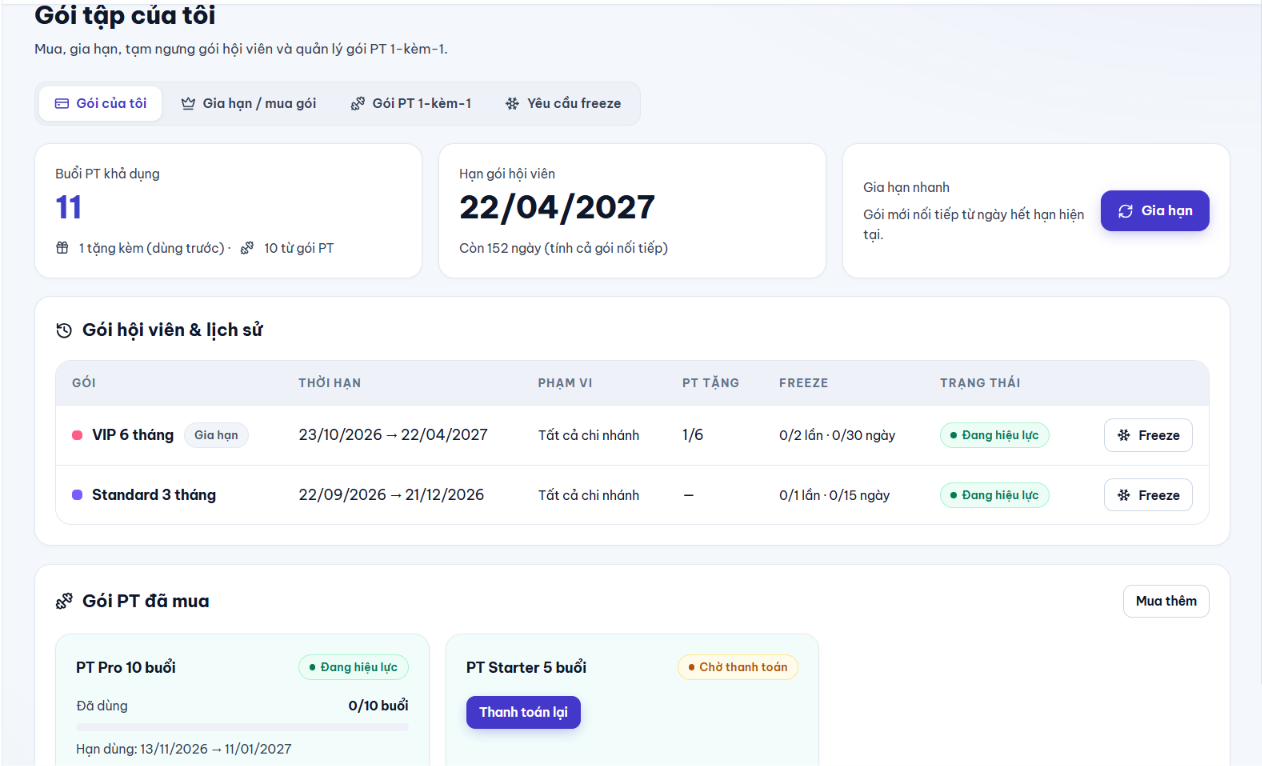
\includegraphics[width=0.92\textwidth]{images/ui_ktpm/membership.png}
\caption{Giao diện màn hình Tổng quan Gói tập của tôi dành cho Hội viên}
\label{fig:membership}
\end{figure}

\par\medskip\noindent\textbf{Danh sách các thành phần giao diện}\par\smallskip
{\footnotesize
\setlength{\tabcolsep}{2.5pt}
\begin{longtable}{|c|L{2.95cm}|L{1.85cm}|L{2.95cm}|L{2.75cm}|L{1.90cm}|L{2.05cm}|}
\hline
\textbf{STT} & \textbf{Tên} & \textbf{Kiểu} & \textbf{Ý nghĩa} & \textbf{Miền giá trị} & \textbf{Giá trị mặc định} & \textbf{Ghi chú} \\
\hline
\endfirsthead
\hline
\textbf{STT} & \textbf{Tên} & \textbf{Kiểu} & \textbf{Ý nghĩa} & \textbf{Miền giá trị} & \textbf{Giá trị mặc định} & \textbf{Ghi chú} \\
\hline
\endhead
\hline
\endfoot
\hline
\caption{Danh sách các thành phần giao diện -- Màn hình Tổng quan Gói tập của tôi} \\
\endlastfoot
1 & \texttt{Tab\_MenuGoiTap} & Tab Group & Chuyển đổi giữa 4 phân mục quản lý gói tập & \{\texttt{"Gói của tôi"}, \texttt{"Gia hạn / mua gói"}, \texttt{"Gói PT 1-kèm-1"}, \texttt{"Yêu cầu freeze"}\} & \texttt{"Gói của tôi"} & Tab \textit{Yêu cầu freeze} kèm số đơn chờ \\ \hline
2 & \texttt{Card\_BuoiPT} & Card Panel & Hiển thị tổng số buổi PT 1-kèm-1 khả dụng (tặng kèm và gói PT) & Số nguyên $\ge 0$ & Theo số dư hiện tại & Ưu tiên trừ buổi tặng kèm trước \\ \hline
3 & \texttt{Card\_HanHoiVien} & Card Panel & Hiển thị ngày hết hạn xa nhất và số ngày còn lại của gói hội viên & Ngày hợp lệ (\texttt{dd/MM/yyyy}) & Theo gói đã thanh toán & Tính gộp các gói nối tiếp \\ \hline
4 & \texttt{Btn\_GiaHanNhanh} & Button & Điều hướng nhanh sang tab danh mục gia hạn gói tập & Kích hoạt & \texttt{"Gia hạn"} & Nút hành động chính \\ \hline
5 & \texttt{Grd\_GoiHoiVien} & DataGrid & Bảng danh sách gói hội viên đã mua (thời hạn, phạm vi, PT tặng, quota Freeze, trạng thái) & Bản ghi từ \texttt{Memberships} & Sắp giảm dần theo ngày bắt đầu & Có cột nút thao tác cuối dòng \\ \hline
6 & \texttt{Btn\_FreezeGoi} & Button & Mở hộp thoại gửi yêu cầu tạm ngưng (\textit{Freeze}) cho gói tương ứng & Kích hoạt khi gói còn hạn và còn quota & \texttt{"Freeze"} & Ẩn với gói không hỗ trợ Freeze \\ \hline
7 & \texttt{Card\_GoiPTDaMua} & Card Group & Nhóm thẻ hiển thị tiến độ sử dụng và thời hạn các gói PT đã mua & Danh sách các gói PT từ \texttt{Memberships} & Theo hội viên đăng nhập & Kèm thanh tiến độ số buổi \\* \hline
8 & \texttt{Btn\_ThanhToanLai} & Button & Mở lại hộp thoại thanh toán cho các gói đang ở trạng thái \textit{Chờ thanh toán} & Kích hoạt khi \texttt{pending\_payment} & \texttt{"Thanh toán lại"} & Tái kích hoạt đơn hàng treo \\ \hline
\end{longtable}
}

\par\medskip\noindent\textbf{Danh sách các biến cố}\par\smallskip
{\footnotesize
\setlength{\tabcolsep}{4pt}
\begin{longtable}{|c|L{3.5cm}|L{7.8cm}|L{3.5cm}|}
\hline
\textbf{STT} & \textbf{Điều kiện kích hoạt} & \textbf{Xử lý} & \textbf{Ghi chú} \\
\hline
\endfirsthead
\hline
\textbf{STT} & \textbf{Điều kiện kích hoạt} & \textbf{Xử lý} & \textbf{Ghi chú} \\
\hline
\endhead
\hline
\endfoot
\hline
\caption{Danh sách các biến cố -- Màn hình Tổng quan Gói tập của tôi} \\
\endlastfoot
0 & Khởi động màn hình (\texttt{/member/memberships}) & Truy vấn danh sách gói hội viên từ \texttt{Memberships}, gói PT đã mua và yêu cầu Freeze của người dùng; tính tổng số buổi PT khả dụng lên \texttt{Card\_BuoiPT}, ngày hết hạn nối tiếp xa nhất lên \texttt{Card\_HanHoiVien} và kết xuất \texttt{Grd\_GoiHoiVien}, \texttt{Card\_GoiPTDaMua}. & Tự động tính trạng thái hiệu lực từng gói. \\ \hline
1 & Nhấn nút \texttt{Btn\_GiaHanNhanh} (\textit{Gia hạn}) & Chuyển tab hiện hành trên \texttt{Tab\_MenuGoiTap} sang \textit{Gia hạn / mua gói} để hiển thị danh sách gói hội viên đang mở bán. & Rút ngắn thao tác mua nối tiếp. \\ \hline
2 & Nhấn nút \texttt{Btn\_FreezeGoi} (\textit{Freeze}) tại một dòng gói tập & Kiểm tra hạn mức số lần và số ngày Freeze còn lại của gói; nếu đủ điều kiện, mở hộp thoại nhập ngày bắt đầu, số ngày tạm ngưng và lý do để gửi yêu cầu cho Lễ tân duyệt. & Cảnh báo các lịch tập bị hủy tự động nếu trùng khoảng Freeze. \\ \hline
3 & Nhấn nút \texttt{Btn\_ThanhToanLai} (\textit{Thanh toán lại}) & Khôi phục thông tin đơn hàng chưa hoàn tất và mở lại \textit{Hộp thoại Thanh toán Trực tuyến} để hội viên thực hiện thanh toán tiếp. & Áp dụng cho cả gói hội viên và gói PT. \\* \hline
4 & Chuyển tab trên \texttt{Tab\_MenuGoiTap} hoặc nhấn \textit{Mua thêm} & Cập nhật giao diện nội dung tương ứng theo tab được chọn (\textit{Gia hạn / mua gói}, \textit{Gói PT 1-kèm-1}, hoặc \textit{Yêu cầu freeze}). & Giữ nguyên dữ liệu đã tải. \\ \hline
\end{longtable}
}

% --- 6.3.2 DANH MỤC GIA HẠN / MUA GÓI HỘI VIÊN ---
\subsubsection{Màn hình Danh mục Gia hạn / Mua gói Hội viên (Hội viên)}
Màn hình \textbf{Danh mục Gia hạn / Mua gói Hội viên} (đường dẫn \texttt{/member/memberships}, tab \textit{Gia hạn / mua gói}) cho phép \textbf{Hội viên} duyệt các gói tập đang phát hành kèm đơn giá quy đổi theo tháng, phạm vi chi nhánh, quyền lợi lớp nhóm/PT tặng kèm và tự động tính ngày hiệu lực nối tiếp sau ngày hết hạn của gói hiện tại.

\begin{figure}[H]
\centering
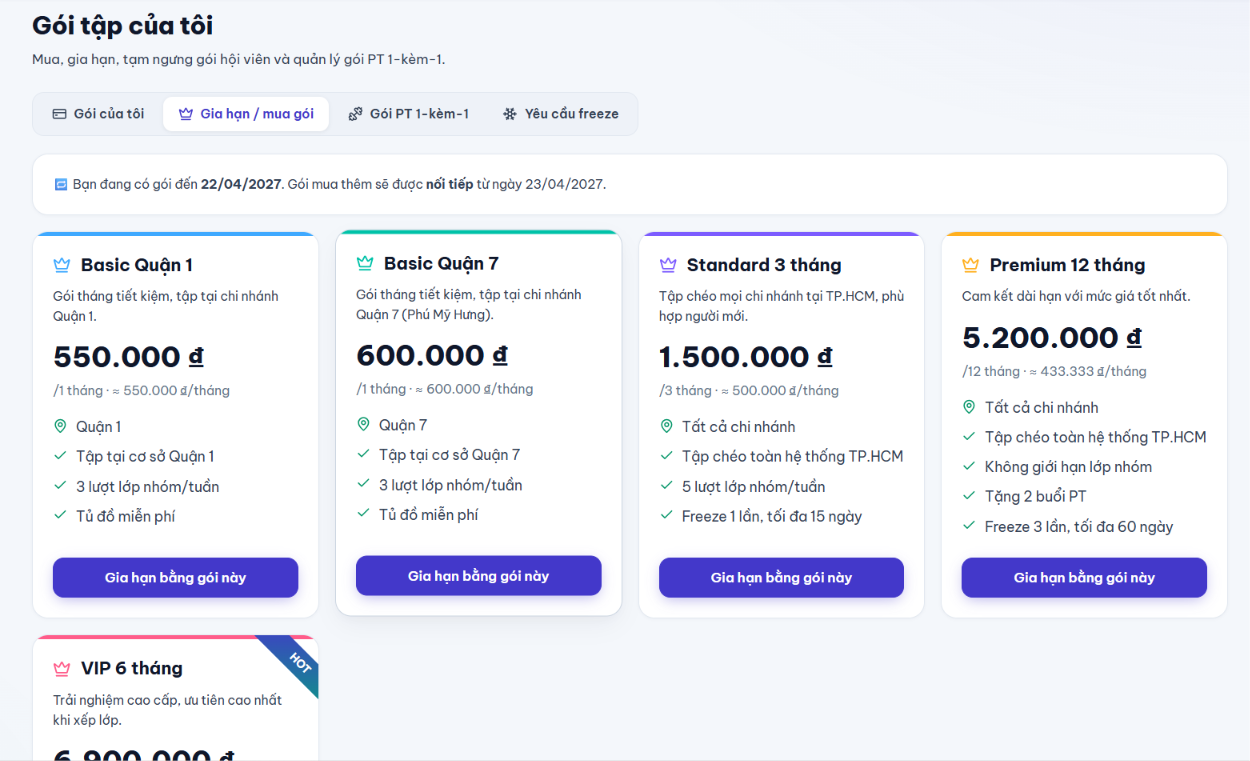
\includegraphics[width=0.92\textwidth]{images/ui_ktpm/giahangoimua.png}
\caption{Giao diện màn hình Danh mục Gia hạn / Mua gói Hội viên}
\label{fig:giahangoimua}
\end{figure}

\par\medskip\noindent\textbf{Danh sách các thành phần giao diện}\par\smallskip
{\footnotesize
\setlength{\tabcolsep}{2.5pt}
\begin{longtable}{|c|L{2.95cm}|L{1.85cm}|L{2.95cm}|L{2.75cm}|L{1.90cm}|L{2.05cm}|}
\hline
\textbf{STT} & \textbf{Tên} & \textbf{Kiểu} & \textbf{Ý nghĩa} & \textbf{Miền giá trị} & \textbf{Giá trị mặc định} & \textbf{Ghi chú} \\
\hline
\endfirsthead
\hline
\textbf{STT} & \textbf{Tên} & \textbf{Kiểu} & \textbf{Ý nghĩa} & \textbf{Miền giá trị} & \textbf{Giá trị mặc định} & \textbf{Ghi chú} \\
\hline
\endhead
\hline
\endfoot
\hline
\caption{Danh sách các thành phần giao diện -- Màn hình Danh mục Gia hạn / Mua gói Hội viên} \\
\endlastfoot
1 & \texttt{Pnl\_NgayNoiTiep} & Alert Panel & Thông báo ngày hết hạn hiện tại và thời điểm bắt đầu hiệu lực nối tiếp (\texttt{endDate + 1}) & Hiển thị khi hội viên đã có gói hiệu lực & Tự động tính từ gói gần nhất & Tránh mất ngày tập khi gia hạn sớm \\ \hline
2 & \texttt{Card\_GoiHoiVien} & Card Grid & Lưới thẻ các gói hội viên đang mở bán (giá, thời hạn, phạm vi, quyền lợi, dải màu) & Bản ghi từ \texttt{Membership\_Plans} (\texttt{active}) & Tất cả gói đang hoạt động & Gắn nhãn \texttt{HOT} cho gói ưu tiên cấp 3 \\ \hline
3 & \texttt{Lbl\_\hspace{0pt}GiaQuyDoi} & Label & Hiển thị thời hạn tháng và đơn giá quy đổi trung bình mỗi tháng & Chuỗi tiền tệ (VNĐ/tháng) & \texttt{price /\hspace{0pt} duration\hspace{0pt}Months} & Hỗ trợ hội viên so sánh chi phí \\* \hline
4 & \texttt{Btn\_ChonGoiHV} & Button & Chọn gói hội viên để chọn chi nhánh (nếu đa chi nhánh) và mở hộp thoại thanh toán & \{\texttt{"Gia hạn bằng gói này"}, \texttt{"Mua ngay"}\} & Theo trạng thái gói hiện có & Nút hành động chính trên từng thẻ \\ \hline
\end{longtable}
}

\par\medskip\noindent\textbf{Danh sách các biến cố}\par\smallskip
{\footnotesize
\setlength{\tabcolsep}{4pt}
\begin{longtable}{|c|L{3.5cm}|L{7.8cm}|L{3.5cm}|}
\hline
\textbf{STT} & \textbf{Điều kiện kích hoạt} & \textbf{Xử lý} & \textbf{Ghi chú} \\
\hline
\endfirsthead
\hline
\textbf{STT} & \textbf{Điều kiện kích hoạt} & \textbf{Xử lý} & \textbf{Ghi chú} \\
\hline
\endhead
\hline
\endfoot
\hline
\caption{Danh sách các biến cố -- Màn hình Danh mục Gia hạn / Mua gói Hội viên} \\
\endlastfoot
0 & Khởi động / Chọn tab \textit{Gia hạn / mua gói} & Truy vấn ngày hết hạn xa nhất của hội viên để tính ngày hiệu lực nối tiếp (\texttt{Ngày cũ + 1}) lên \texttt{Pnl\_NgayNoiTiep}; lọc các gói trong \texttt{Membership\_Plans} có trạng thái hoạt động để hiển thị lên \texttt{Card\_GoiHoiVien}. & Tính toán tự động phía nghiệp vụ. \\ \hline
1 & Nhấn \texttt{Btn\_ChonGoiHV} trên một thẻ gói tập & Kiểm tra phạm vi chi nhánh của gói: nếu chỉ áp dụng tại 1 chi nhánh thì mở thẳng \textit{Hộp thoại Thanh toán Trực tuyến}; nếu áp dụng nhiều chi nhánh thì mở hộp thoại chọn chi nhánh đăng ký trước khi thanh toán. & Ghi nhận chi nhánh cho báo cáo doanh thu. \\* \hline
2 & Chọn chi nhánh trong hộp thoại phụ (nếu có) & Đóng hộp thoại chọn chi nhánh, gán thông tin gói, chi nhánh và ngày bắt đầu hiệu lực rồi chuyển sang \textit{Hộp thoại Thanh toán Trực tuyến}. & Cho phép chuyển bước thanh toán liền mạch. \\ \hline
\end{longtable}
}

% --- 6.3.3 DANH MỤC GÓI HUẤN LUYỆN VIÊN CÁ NHÂN 1-KÈM-1 ---
\subsubsection{Màn hình Danh mục Gói Huấn luyện viên Cá nhân 1-kèm-1 (Hội viên)}
Màn hình \textbf{Danh mục Gói Huấn luyện viên Cá nhân 1-kèm-1} (đường dẫn \texttt{/member/\hspace{0pt}memberships}, tab \textit{Gói PT 1-kèm-1}) cho phép \textbf{Hội viên} tham khảo quy chế bảo lưu buổi PT và lựa chọn mua các gói huấn luyện cá nhân theo số buổi và thời hạn sử dụng.

\begin{figure}[H]
\centering
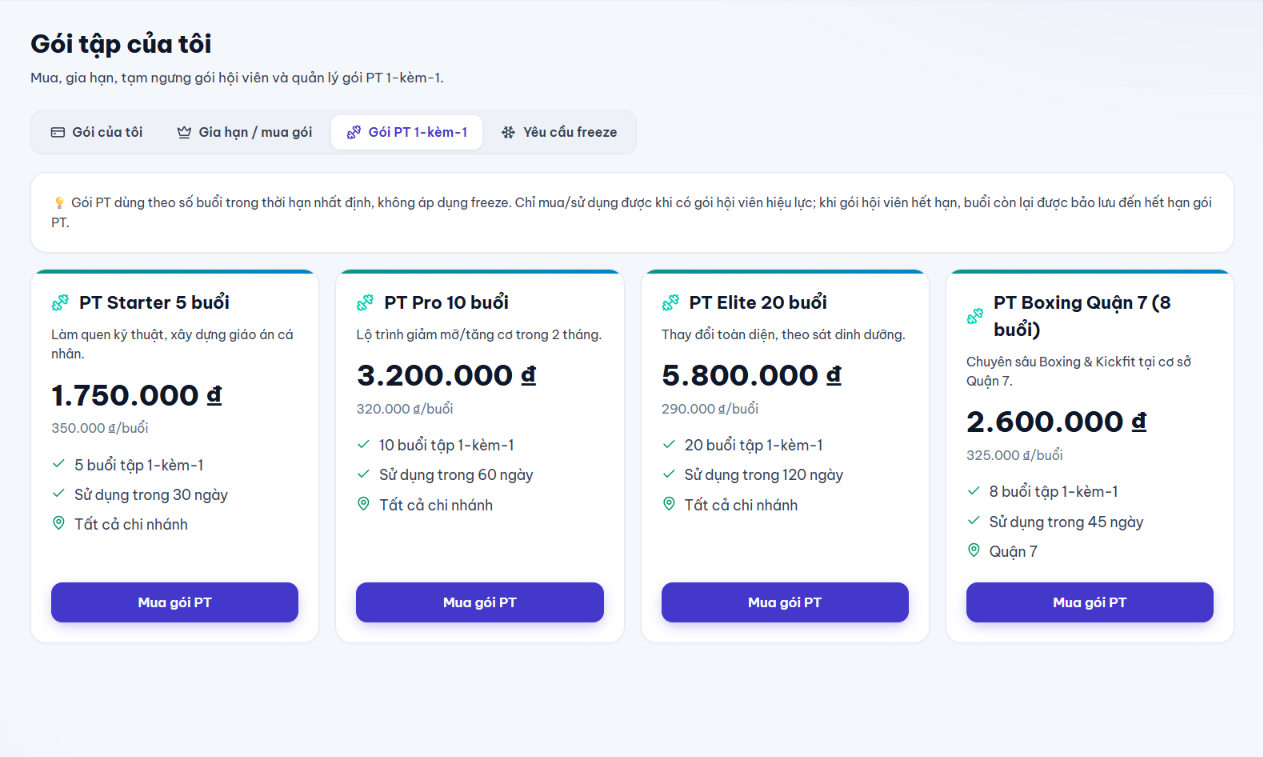
\includegraphics[width=0.92\textwidth]{images/ui_ktpm/goipt.png}
\caption{Giao diện màn hình Danh mục Gói Huấn luyện viên Cá nhân 1-kèm-1}
\label{fig:goipt}
\end{figure}

\par\medskip\noindent\textbf{Danh sách các thành phần giao diện}\par\smallskip
{\footnotesize
\setlength{\tabcolsep}{2.5pt}
\begin{longtable}{|c|L{2.95cm}|L{1.85cm}|L{2.95cm}|L{2.75cm}|L{1.90cm}|L{2.05cm}|}
\hline
\textbf{STT} & \textbf{Tên} & \textbf{Kiểu} & \textbf{Ý nghĩa} & \textbf{Miền giá trị} & \textbf{Giá trị mặc định} & \textbf{Ghi chú} \\
\hline
\endfirsthead
\hline
\textbf{STT} & \textbf{Tên} & \textbf{Kiểu} & \textbf{Ý nghĩa} & \textbf{Miền giá trị} & \textbf{Giá trị mặc định} & \textbf{Ghi chú} \\
\hline
\endhead
\hline
\endfoot
\hline
\caption{Danh sách các thành phần giao diện -- Màn hình Danh mục Gói PT 1-kèm-1} \\
\endlastfoot
1 & \texttt{Pnl\_QuyDinhPT} & Alert Panel & Hiển thị quy định: gói PT không áp dụng Freeze và yêu cầu có gói hội viên còn hiệu lực & Văn bản cố định & Luôn hiển thị đầu tab & Minh bạch điều kiện bảo lưu buổi \\ \hline
2 & \texttt{Card\_GoiPT} & Card Grid & Lưới thẻ các gói PT đang mở bán (tên gói, mô tả, số buổi, hạn ngày, phạm vi) & Các gói PT có trạng thái \texttt{active} & Tất cả gói PT khả dụng & Phân loại theo nhu cầu và chi nhánh \\ \hline
3 & \texttt{Lbl\_DonGiaBuoi} & Label & Hiển thị đơn giá trung bình cho mỗi buổi tập 1-kèm-1 & Chuỗi tiền tệ (VNĐ/buổi) & \texttt{price / sessions} & Tính toán tự động \\* \hline
4 & \texttt{Btn\_MuaGoiPT} & Button & Kích hoạt luồng kiểm tra điều kiện và thanh toán mua gói PT & \{\texttt{"Mua gói PT"}, \texttt{"Cần gói hội viên hiệu lực"}\} & Tùy hiệu lực gói hội viên & Vô hiệu hóa nếu chưa có gói hội viên \\ \hline
\end{longtable}
}

\par\medskip\noindent\textbf{Danh sách các biến cố}\par\smallskip
{\footnotesize
\setlength{\tabcolsep}{4pt}
\begin{longtable}{|c|L{3.5cm}|L{7.8cm}|L{3.5cm}|}
\hline
\textbf{STT} & \textbf{Điều kiện kích hoạt} & \textbf{Xử lý} & \textbf{Ghi chú} \\
\hline
\endfirsthead
\hline
\textbf{STT} & \textbf{Điều kiện kích hoạt} & \textbf{Xử lý} & \textbf{Ghi chú} \\
\hline
\endhead
\hline
\endfoot
\hline
\caption{Danh sách các biến cố -- Màn hình Danh mục Gói PT 1-kèm-1} \\
\endlastfoot
0 & Khởi động / Chọn tab \textit{Gói PT 1-kèm-1} & Tải danh sách gói PT đang mở bán, tính đơn giá trung bình mỗi buổi và kiểm tra xem hội viên có gói hội viên hiệu lực hay không để thiết lập trạng thái khả dụng cho \texttt{Btn\_MuaGoiPT}. & Vô hiệu hóa nút mua nếu gói hội viên hết hạn. \\ \hline
1 & Nhấn \texttt{Btn\_MuaGoiPT} khi đủ điều kiện gói hội viên & Kiểm tra lại hiệu lực gói hội viên; xác định chi nhánh áp dụng (mở hộp thoại chọn chi nhánh nếu gói hỗ trợ đa chi nhánh) rồi mở \textit{Hộp thoại Thanh toán Trực tuyến}. & Chuyển tiếp sang bước thanh toán. \\* \hline
2 & Thao tác khi không có gói hội viên hiệu lực & Hệ thống giữ nút ở trạng thái vô hiệu hóa hoặc báo lỗi yêu cầu hội viên mua/gia hạn gói hội viên trước khi mua gói PT. & Thực thi đúng quy tắc nghiệp vụ ràng buộc. \\ \hline
\end{longtable}
}

% --- 6.3.4 HỘP THOẠI THANH TOÁN TRỰC TUYẾN ---
\subsubsection{Hộp thoại Thanh toán Trực tuyến (Hội viên)}
\textbf{Hộp thoại Thanh toán Trực tuyến} (\texttt{PaymentModal}) xuất hiện dưới dạng cửa sổ nổi khi \textbf{Hội viên} thực hiện mua mới, gia hạn hoặc thanh toán lại đơn hàng gói tập, cho phép kiểm tra tóm tắt hóa đơn, chọn phương thức thanh toán và xử lý cả trường hợp thành công lẫn mô phỏng giao dịch thất bại.

\begin{figure}[H]
\centering
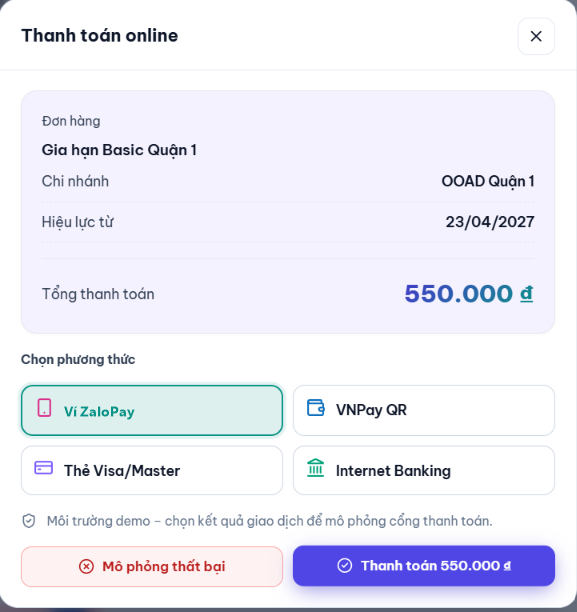
\includegraphics[width=0.58\textwidth]{images/ui_ktpm/thanhtoangoi.png}
\caption{Giao diện Hộp thoại Thanh toán Trực tuyến}
\label{fig:thanhtoangoi}
\end{figure}

\par\medskip\noindent\textbf{Danh sách các thành phần giao diện}\par\smallskip
{\footnotesize
\setlength{\tabcolsep}{2.5pt}
\begin{longtable}{|c|L{2.95cm}|L{1.85cm}|L{2.95cm}|L{2.75cm}|L{1.90cm}|L{2.05cm}|}
\hline
\textbf{STT} & \textbf{Tên} & \textbf{Kiểu} & \textbf{Ý nghĩa} & \textbf{Miền giá trị} & \textbf{Giá trị mặc định} & \textbf{Ghi chú} \\
\hline
\endfirsthead
\hline
\textbf{STT} & \textbf{Tên} & \textbf{Kiểu} & \textbf{Ý nghĩa} & \textbf{Miền giá trị} & \textbf{Giá trị mặc định} & \textbf{Ghi chú} \\
\hline
\endhead
\hline
\endfoot
\hline
\caption{Danh sách các thành phần giao diện -- Hộp thoại Thanh toán Trực tuyến} \\
\endlastfoot
1 & \texttt{Lbl\_TenDonHang} & Label & Tên gói hội viên hoặc gói PT đang thanh toán & Chuỗi ký tự & Theo gói đã chọn & Ví dụ: \texttt{Gia hạn Basic Quận 1} \\ \hline
2 & \texttt{Lbl\_ChiNhanhTT} & Label & Chi nhánh phòng tập ghi nhận giao dịch & Tên chi nhánh & Chi nhánh đã chọn & Chỉ đọc \\ \hline
3 & \texttt{Lbl\_NgayHieuLuc} & Label & Ngày bắt đầu hiệu lực hoặc số buổi/thời hạn của gói & Ngày hoặc số buổi & Theo thông tin đơn hàng & Tính nối tiếp nếu gia hạn \\ \hline
4 & \texttt{Lbl\_TongTienTT} & Label & Tổng số tiền thanh toán của giao dịch & Số tiền (VNĐ) & Giá niêm yết của gói & Định dạng tiền tệ Việt Nam \\ \hline
5 & \texttt{Opt\_PhuongThucTT} & Radio Group & Chọn 1 trong 4 cổng thanh toán trực tuyến & \{\texttt{"Ví ZaloPay"}, \texttt{"VNPay QR"}, \texttt{"Thẻ Visa/Master"}, \texttt{"Internet Banking"}\} & \texttt{"Ví ZaloPay"} & Có viền sáng nổi bật mục chọn \\ \hline
6 & \texttt{Btn\_ThanhToanTT} & Button & Thực hiện xác nhận thanh toán thành công và kích hoạt gói & Kích hoạt & \texttt{"Thanh toán <Số tiền>"} & Nút hành động chính \\ \hline
7 & \texttt{Btn\_MoPhongLoi} & Button & Mô phỏng ngoại lệ giao dịch thất bại (hết số dư, lỗi cổng) & Kích hoạt & \texttt{"Mô phỏng thất bại"} & Phục vụ kiểm thử luồng lỗi \\* \hline
8 & \texttt{Btn\_DongTT} & Button & Hủy thao tác và đóng hộp thoại thanh toán & Kích hoạt & \texttt{"$\times$"} & Không làm thay đổi dữ liệu \\ \hline
\end{longtable}
}

\par\medskip\noindent\textbf{Danh sách các biến cố}\par\smallskip
{\footnotesize
\setlength{\tabcolsep}{4pt}
\begin{longtable}{|c|L{3.5cm}|L{7.8cm}|L{3.5cm}|}
\hline
\textbf{STT} & \textbf{Điều kiện kích hoạt} & \textbf{Xử lý} & \textbf{Ghi chú} \\
\hline
\endfirsthead
\hline
\textbf{STT} & \textbf{Điều kiện kích hoạt} & \textbf{Xử lý} & \textbf{Ghi chú} \\
\hline
\endhead
\hline
\endfoot
\hline
\caption{Danh sách các biến cố -- Hộp thoại Thanh toán Trực tuyến} \\
\endlastfoot
0 & Mở hộp thoại Thanh toán Trực tuyến & Nạp thông tin đơn hàng (tên gói, chi nhánh, hiệu lực từ hoặc số buổi, tổng tiền) lên phần tóm tắt; đặt phương thức mặc định là \textit{Ví ZaloPay}. & Sẵn sàng chọn kênh thanh toán. \\ \hline
1 & Nhấn chọn một phương thức trên \texttt{Opt\_PhuongThucTT} & Cập nhật phương thức thanh toán đang chọn và tô viền xanh nổi bật vào thẻ phương thức tương ứng. & Phản hồi trực quan tức thì. \\ \hline
2 & Nhấn nút \texttt{Btn\_ThanhToanTT} (\textit{Thanh toán}) & Ghi nhận giao dịch trạng thái \texttt{Thành công} vào bảng \texttt{Payments}, kích hoạt gói trong \texttt{Memberships} (bao gồm gói hội viên và nhóm gói PT), gửi thông báo, đóng hộp thoại và chuyển về tab \textit{Gói của tôi}. & Hỗ trợ cả đơn mới và thanh toán lại. \\ \hline
3 & Nhấn nút \texttt{Btn\_MoPhongLoi} (\textit{Mô phỏng thất bại}) & Lưu giao dịch trạng thái \texttt{Thất bại} vào \texttt{Payments}, giữ gói tập ở trạng thái \texttt{pending\_payment}, hiển thị Toast cảnh báo lỗi và đóng hộp thoại. & Cho phép hội viên nhấn \textit{Thanh toán lại} sau. \\* \hline
4 & Nhấn nút \texttt{Btn\_DongTT} (\texttt{$\times$}) & Đóng hộp thoại và giữ nguyên trạng thái trước khi mở thanh toán. & An toàn, không sinh giao dịch rác. \\ \hline
\end{longtable}
}

% --- 6.3.5 LỊCH SỬ GIAO DỊCH ---
\subsubsection{Màn hình Báo biểu Lịch sử Giao dịch (Hội viên)}
Màn hình \textbf{Báo biểu Lịch sử Giao dịch} (đường dẫn \texttt{/member/payments}) cho phép \textbf{Hội viên} tra cứu toàn bộ nhật ký giao dịch mua mới hoặc gia hạn gói tập đã phát sinh, xem tổng số tiền đã thanh toán thành công và phân biệt nhanh kết quả từng giao dịch qua nhãn màu trực quan.

\begin{figure}[H]
\centering
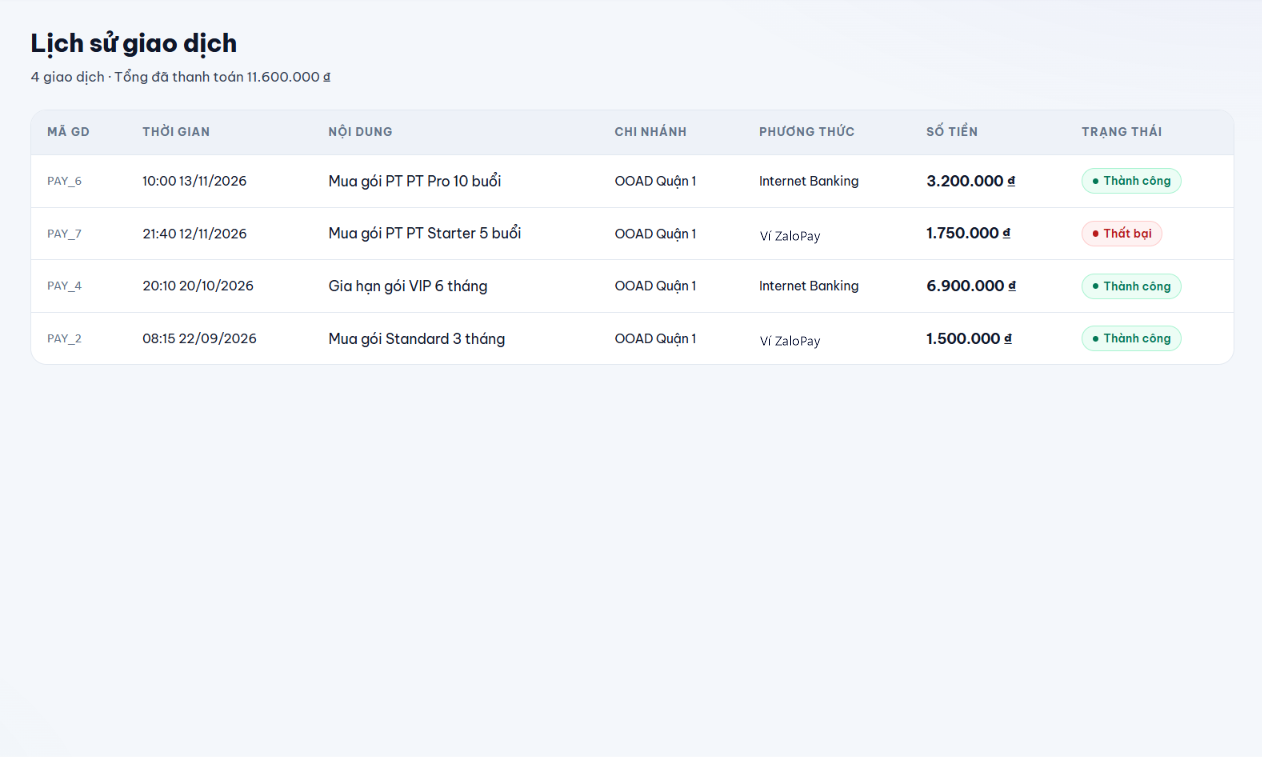
\includegraphics[width=0.92\textwidth]{images/ui_ktpm/lichsugiaodich.png}
\caption{Giao diện màn hình Báo biểu Lịch sử Giao dịch}
\label{fig:lichsugiaodich}
\end{figure}

\par\medskip\noindent\textbf{Danh sách các thành phần giao diện}\par\smallskip
{\footnotesize
\setlength{\tabcolsep}{2.5pt}
\begin{longtable}{|c|L{2.95cm}|L{1.85cm}|L{2.95cm}|L{2.75cm}|L{1.90cm}|L{2.05cm}|}
\hline
\textbf{STT} & \textbf{Tên} & \textbf{Kiểu} & \textbf{Ý nghĩa} & \textbf{Miền giá trị} & \textbf{Giá trị mặc định} & \textbf{Ghi chú} \\
\hline
\endfirsthead
\hline
\textbf{STT} & \textbf{Tên} & \textbf{Kiểu} & \textbf{Ý nghĩa} & \textbf{Miền giá trị} & \textbf{Giá trị mặc định} & \textbf{Ghi chú} \\
\hline
\endhead
\hline
\endfoot
\hline
\caption{Danh sách các thành phần giao diện -- Màn hình Báo biểu Lịch sử Giao dịch} \\
\endlastfoot
1 & \texttt{Lbl\_TongGiaoDich} & Label & Dòng tóm tắt tổng số lượng giao dịch và tổng số tiền đã thanh toán thành công & Chuỗi tổng hợp số GD và tổng tiền VNĐ & Tính từ bảng \texttt{Payments} & Tự động loại trừ các giao dịch thất bại \\ \hline
2 & \texttt{Grd\_GiaoDich} & DataGrid & Bảng 7 cột (\textit{Mã GD}, \textit{Thời gian}, \textit{Nội dung}, \textit{Chi nhánh}, \textit{Phương thức}, \textit{Số tiền}, \textit{Trạng thái}) & Danh sách bản ghi của hội viên từ \texttt{Payments} & Toàn bộ giao dịch cá nhân & Hiển thị Empty State nếu chưa có giao dịch \\* \hline
3 & \texttt{Bdg\_TrangThaiGD} & Badge & Nhãn màu phân biệt kết quả thanh toán của từng dòng & \{\texttt{"Thành công"}, \texttt{"Thất bại"}\} & Theo trạng thái bản ghi & Xanh lá: Thành công; Đỏ: Thất bại \\ \hline
\end{longtable}
}

\par\medskip\noindent\textbf{Danh sách các biến cố}\par\smallskip
{\footnotesize
\setlength{\tabcolsep}{4pt}
\begin{longtable}{|c|L{3.5cm}|L{7.8cm}|L{3.5cm}|}
\hline
\textbf{STT} & \textbf{Điều kiện kích hoạt} & \textbf{Xử lý} & \textbf{Ghi chú} \\
\hline
\endfirsthead
\hline
\textbf{STT} & \textbf{Điều kiện kích hoạt} & \textbf{Xử lý} & \textbf{Ghi chú} \\
\hline
\endhead
\hline
\endfoot
\hline
\caption{Danh sách các biến cố -- Màn hình Báo biểu Lịch sử Giao dịch} \\
\endlastfoot
0 & Khởi động màn hình (\texttt{/member/payments}) & Truy vấn toàn bộ giao dịch thuộc người dùng hiện tại từ bảng \texttt{Payments}; tính tổng số tiền các giao dịch có trạng thái \texttt{success} để hiển thị lên \texttt{Lbl\_TongGiaoDich} và kết xuất dữ liệu lên \texttt{Grd\_GiaoDich}. & Chỉ hiển thị giao dịch của chính hội viên đăng nhập. \\ \hline
1 & Danh sách giao dịch trống & Khi hội viên chưa phát sinh giao dịch nào, ẩn bảng \texttt{Grd\_GiaoDich} và hiển thị khối trạng thái rỗng kèm biểu tượng hóa đơn và thông báo \textit{``Chưa có giao dịch''}. & Tránh hiển thị bảng trắng gây nhầm lẫn. \\* \hline
2 & Có giao dịch mới phát sinh từ trang Gói tập & Khi người dùng thực hiện mua/gia hạn xong và quay lại \texttt{/member/payments}, bảng tự động cập nhật mã giao dịch mới, phương thức, số tiền và nhãn \texttt{Bdg\_TrangThaiGD}. & Bao gồm cả các giao dịch thất bại để đối soát. \\ \hline
\end{longtable}
}

% --- 6.3.6 TRẠNG THÁI YÊU CẦU FREEZE ---
\subsubsection{Màn hình Trạng thái Yêu cầu Freeze (Hội viên)}
Màn hình \textbf{Trạng thái Yêu cầu Freeze} (đường dẫn \texttt{/member/memberships}, tab \textit{Yêu cầu freeze}) giúp \textbf{Hội viên} theo dõi lịch sử các đơn xin tạm ngưng gói tập đã gửi (ngày gửi, gói áp dụng, khoảng nghỉ, lý do, trạng thái duyệt và phản hồi của lễ tân) hoặc hiển thị trạng thái rỗng hướng dẫn khi chưa có đơn nào.

\begin{figure}[H]
\centering
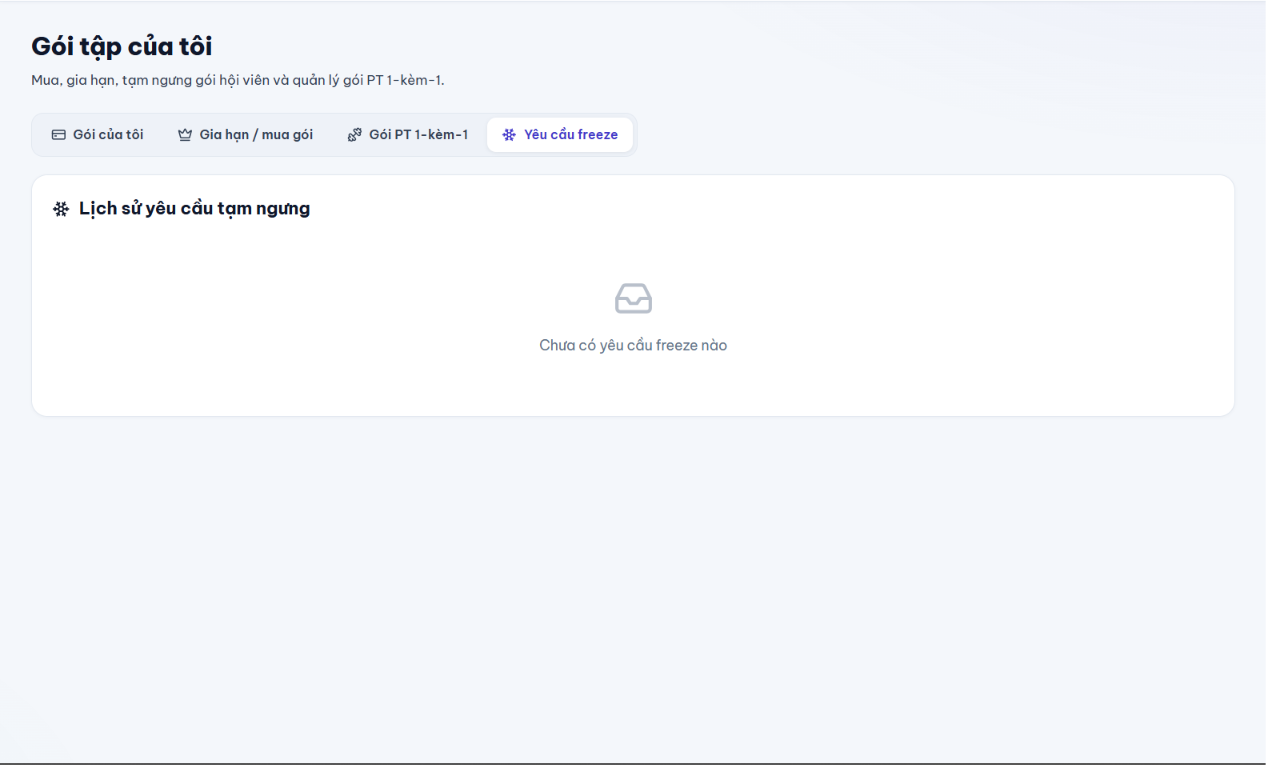
\includegraphics[width=0.92\textwidth]{images/ui_ktpm/yeucaufreeze.png}
\caption{Giao diện màn hình Trạng thái Yêu cầu Freeze của Hội viên}
\label{fig:yeucaufreeze}
\end{figure}

\par\medskip\noindent\textbf{Danh sách các thành phần giao diện}\par\smallskip
{\footnotesize
\setlength{\tabcolsep}{2.5pt}
\begin{longtable}{|c|L{2.95cm}|L{1.85cm}|L{2.95cm}|L{2.75cm}|L{1.90cm}|L{2.05cm}|}
\hline
\textbf{STT} & \textbf{Tên} & \textbf{Kiểu} & \textbf{Ý nghĩa} & \textbf{Miền giá trị} & \textbf{Giá trị mặc định} & \textbf{Ghi chú} \\
\hline
\endfirsthead
\hline
\textbf{STT} & \textbf{Tên} & \textbf{Kiểu} & \textbf{Ý nghĩa} & \textbf{Miền giá trị} & \textbf{Giá trị mặc định} & \textbf{Ghi chú} \\
\hline
\endhead
\hline
\endfoot
\hline
\caption{Danh sách các thành phần giao diện -- Màn hình Trạng thái Yêu cầu Freeze} \\
\endlastfoot
1 & \texttt{Tab\_YeuCauFreeze} & Tab Group & Chuyển đến phân mục lịch sử yêu cầu tạm ngưng gói tập & Đang chọn / Không chọn & Đang chọn (Active) & Hiển thị số đơn đang chờ duyệt \\ \hline
2 & \texttt{Pnl\_TrangThaiRong} & Empty State & Hiển thị biểu tượng hộp hồ sơ rỗng và thông báo \textit{``Chưa có yêu cầu freeze nào''} & Hiển thị khi danh sách rỗng & Hiện khi chưa có đơn Freeze & Giúp người dùng nhận biết rõ trạng thái \\ \hline
3 & \texttt{Grd\_LichSuFreeze} & DataGrid & Bảng 7 cột (\textit{Gửi lúc}, \textit{Gói}, \textit{Khoảng tạm ngưng}, \textit{Số ngày}, \textit{Lý do}, \textit{Trạng thái}, \textit{Phản hồi}) & Bản ghi từ \texttt{Freeze\_Requests} & Ẩn khi rỗng & Hiện khi hội viên đã từng gửi đơn \\* \hline
4 & \texttt{Bdg\_\hspace{0pt}TrangThaiFreeze} & Badge & Nhãn trạng thái xử lý của từng đơn Freeze & \{\texttt{"Chờ duyệt"}, \texttt{"Đã duyệt"}, \texttt{"Từ chối"}\} & Theo bản ghi CSDL & Vàng: Chờ duyệt; Xanh: Duyệt; Đỏ: Từ chối \\ \hline
\end{longtable}
}

\par\medskip\noindent\textbf{Danh sách các biến cố}\par\smallskip
{\footnotesize
\setlength{\tabcolsep}{4pt}
\begin{longtable}{|c|L{3.5cm}|L{7.8cm}|L{3.5cm}|}
\hline
\textbf{STT} & \textbf{Điều kiện kích hoạt} & \textbf{Xử lý} & \textbf{Ghi chú} \\
\hline
\endfirsthead
\hline
\textbf{STT} & \textbf{Điều kiện kích hoạt} & \textbf{Xử lý} & \textbf{Ghi chú} \\
\hline
\endhead
\hline
\endfoot
\hline
\caption{Danh sách các biến cố -- Màn hình Trạng thái Yêu cầu Freeze} \\
\endlastfoot
0 & Khởi động / Chọn tab \textit{Yêu cầu freeze} & Truy vấn danh sách đơn tạm ngưng của hội viên từ \texttt{Freeze\_Requests}; nếu chưa có đơn nào thì hiển thị \texttt{Pnl\_TrangThaiRong}, ngược lại kết xuất lịch sử lên \texttt{Grd\_LichSuFreeze}. & Cập nhật lại số lượng đơn chờ trên tiêu đề tab. \\ \hline
1 & Hội viên gửi yêu cầu Freeze mới từ tab \textit{Gói của tôi} & Sau khi gửi thành công từ hộp thoại \texttt{FreezeModal}, bản ghi mới trạng thái \texttt{Chờ duyệt} được bổ sung vào danh sách và cập nhật bộ đếm chờ duyệt trên tab. & Đồng thời gửi thông báo cho Lễ tân chi nhánh. \\* \hline
2 & Lễ tân duyệt hoặc từ chối yêu cầu Freeze & Dữ liệu cột \textit{Trạng thái} và \textit{Phản hồi} trên \texttt{Grd\_LichSuFreeze} cập nhật theo kết quả xử lý của lễ tân; nếu được duyệt, hạn gói tập tự động cộng bù ngày. & Hội viên nhận thông báo đẩy kết quả xử lý. \\ \hline
\end{longtable}
}

% --- 6.3.7 TIẾP NHẬN VÀ XỬ LÝ YÊU CẦU FREEZE CHỜ DUYỆT ---
\subsubsection{Màn hình Tiếp nhận và Xử lý Yêu cầu Freeze Chờ duyệt (Nhân viên Lễ tân)}
Màn hình \textbf{Tiếp nhận và Xử lý Yêu cầu Freeze Chờ duyệt} (đường dẫn \texttt{/staff/freeze}, tab \textit{Chờ duyệt}) cung cấp cho \textbf{Nhân viên Lễ tân} thông tin thẩm định đầy đủ trên từng thẻ hồ sơ: thông tin hội viên, gói tập hiện hành, khoảng ngày xin tạm ngưng, hạn mức đã dùng, cảnh báo số lịch hẹn sẽ tự hủy và cặp nút \textit{Duyệt} / \textit{Từ chối}.

\begin{figure}[H]
\centering
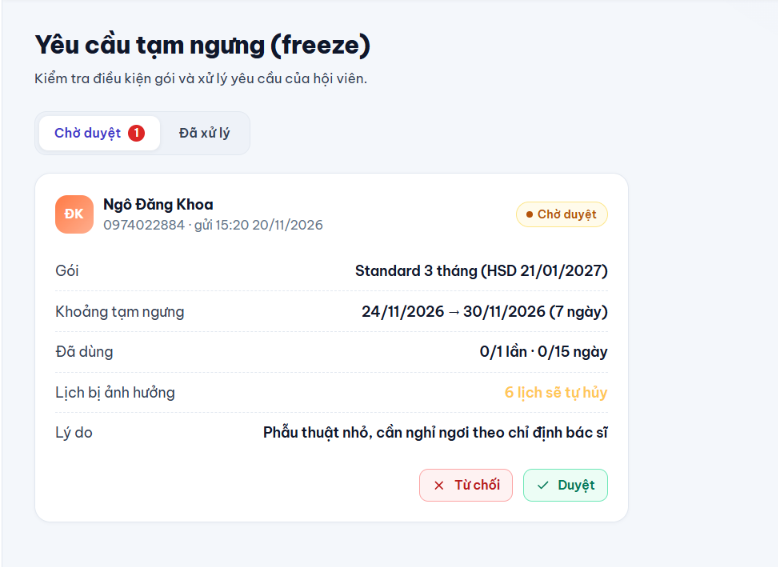
\includegraphics[width=0.92\textwidth]{images/ui_ktpm/letanxulyyeucau.png}
\caption{Giao diện màn hình Tiếp nhận và Xử lý Yêu cầu Freeze Chờ duyệt}
\label{fig:letanxulyyeucau}
\end{figure}

\par\medskip\noindent\textbf{Danh sách các thành phần giao diện}\par\smallskip
{\footnotesize
\setlength{\tabcolsep}{2.5pt}
\begin{longtable}{|c|L{2.95cm}|L{1.85cm}|L{2.95cm}|L{2.75cm}|L{1.90cm}|L{2.05cm}|}
\hline
\textbf{STT} & \textbf{Tên} & \textbf{Kiểu} & \textbf{Ý nghĩa} & \textbf{Miền giá trị} & \textbf{Giá trị mặc định} & \textbf{Ghi chú} \\
\hline
\endfirsthead
\hline
\textbf{STT} & \textbf{Tên} & \textbf{Kiểu} & \textbf{Ý nghĩa} & \textbf{Miền giá trị} & \textbf{Giá trị mặc định} & \textbf{Ghi chú} \\
\hline
\endhead
\hline
\endfoot
\hline
\caption{Danh sách các thành phần giao diện -- Màn hình Xử lý Yêu cầu Freeze Chờ duyệt} \\
\endlastfoot
1 & \texttt{Tab\_\hspace{0pt}ChoDuyetFreeze} & Tab Group & Chuyển giữa danh sách \textit{Chờ duyệt} (kèm huy hiệu số lượng) và \textit{Đã xử lý} & \{\texttt{"Chờ duyệt"}, \texttt{"Đã xử lý"}\} & \texttt{"Chờ duyệt"} & Hiển thị số đơn tồn đọng \\ \hline
2 & \texttt{Card\_\hspace{0pt}HoSoFreeze} & Card Grid & Lưới thẻ chứa thông tin chi tiết từng hồ sơ xin tạm ngưng đang chờ duyệt & Danh sách từ \texttt{Freeze\_Requests} (\texttt{pending}) & Toàn bộ đơn chờ duyệt & Hiện Empty State nếu hết đơn chờ \\ \hline
3 & \texttt{Lbl\_\hspace{0pt}ThongTinHV} & Label Group & Hiển thị ảnh đại diện viết tắt, họ tên, SĐT và thời điểm hội viên gửi yêu cầu & Chuỗi ký tự & Theo thông tin hội viên & Chỉ đọc \\ \hline
4 & \texttt{Lbl\_\hspace{0pt}KhoangTamNgung} & Label & Thời gian xin tạm ngưng (\texttt{startDate $\rightarrow$ endDate}) và tổng số ngày & Khoảng ngày hợp lệ & Theo đơn gửi & Dùng để tính cộng bù hạn gói \\ \hline
5 & \texttt{Lbl\_HanMucFreeze} & Label & Hạn mức Freeze đã dùng trên trần cho phép của gói (\texttt{lần}, \texttt{ngày}) & Tỷ số lần và ngày & Theo gói của hội viên & Hỗ trợ đối soát nhanh điều kiện \\ \hline
6 & \texttt{Pnl\_CanhBaoLich} & Label & Cảnh báo màu cam thông báo số lịch lớp nhóm và PT sẽ tự động hủy khi duyệt & Số nguyên $\ge 0$ lịch bị ảnh hưởng & Tính tự động theo khoảng ngày & Giúp lễ tân cân nhắc trước khi duyệt \\ \hline
7 & \texttt{Btn\_TuChoiFreeze} & Button & Mở hộp thoại nhập lý do và từ chối yêu cầu tạm ngưng & Kích hoạt & \texttt{"Từ chối"} & Nút cảnh báo viền đỏ \\* \hline
8 & \texttt{Btn\_DuyetFreeze} & Button & Chấp thuận yêu cầu, bù hạn gói và hủy các lịch hẹn trùng thời gian Freeze & Kích hoạt & \texttt{"Duyệt"} & Nút xác nhận màu xanh lá \\ \hline
\end{longtable}
}

\par\medskip\noindent\textbf{Danh sách các biến cố}\par\smallskip
{\footnotesize
\setlength{\tabcolsep}{4pt}
\begin{longtable}{|c|L{3.5cm}|L{7.8cm}|L{3.5cm}|}
\hline
\textbf{STT} & \textbf{Điều kiện kích hoạt} & \textbf{Xử lý} & \textbf{Ghi chú} \\
\hline
\endfirsthead
\hline
\textbf{STT} & \textbf{Điều kiện kích hoạt} & \textbf{Xử lý} & \textbf{Ghi chú} \\
\hline
\endhead
\hline
\endfoot
\hline
\caption{Danh sách các biến cố -- Màn hình Xử lý Yêu cầu Freeze Chờ duyệt} \\
\endlastfoot
0 & Khởi động màn hình (\texttt{/staff/freeze}) & Truy vấn danh sách yêu cầu có trạng thái \texttt{pending} từ \texttt{Freeze\_Requests}; đối chiếu bảng \texttt{Bookings} để đếm chính xác số lịch lớp nhóm/PT trùng khoảng ngày tạm ngưng và hiển thị lên \texttt{Card\_HoSoFreeze}. & Mặc định mở tab \textit{Chờ duyệt}. \\ \hline
1 & Nhấn nút \texttt{Btn\_DuyetFreeze} (\textit{Duyệt}) & Chuyển trạng thái đơn sang \texttt{Đã duyệt}; cộng bù đúng số ngày Freeze vào ngày hết hạn gói; tự động hủy các lịch lớp/PT nằm trong khoảng tạm ngưng và hoàn lượt/buổi; ghi nhận mã nhân viên, thời gian xử lý và chuyển hồ sơ sang tab \textit{Đã xử lý}. & Thực thi trong một giao dịch nghiệp vụ đồng bộ. \\* \hline
2 & Nhấn nút \texttt{Btn\_TuChoiFreeze} (\textit{Từ chối}) và xác nhận lý do & Mở \texttt{ReasonModal} yêu cầu nhập lý do từ chối; khi xác nhận, cập nhật trạng thái đơn sang \texttt{Từ chối}, lưu ghi chú lý do, gửi thông báo tới hội viên và giữ nguyên hạn gói. & Chuyển đơn sang tab \textit{Đã xử lý}. \\ \hline
\end{longtable}
}

% --- 6.3.8 NHẬT KÝ YÊU CẦU FREEZE ĐÃ XỬ LÝ ---
\subsubsection{Màn hình Nhật ký Yêu cầu Freeze Đã xử lý (Nhân viên Lễ tân)}
Màn hình \textbf{Nhật ký Yêu cầu Freeze Đã xử lý} (đường dẫn \texttt{/staff/freeze}, tab \textit{Đã xử lý}) đóng vai trò lưu vết kiểm toán (\textit{Audit Trail}) cho \textbf{Nhân viên Lễ tân}, hiển thị đầy đủ các yêu cầu đã phê duyệt hoặc từ chối kèm họ tên nhân viên thẩm định, mốc thời gian xử lý và ghi chú phản hồi.

\begin{figure}[H]
\centering
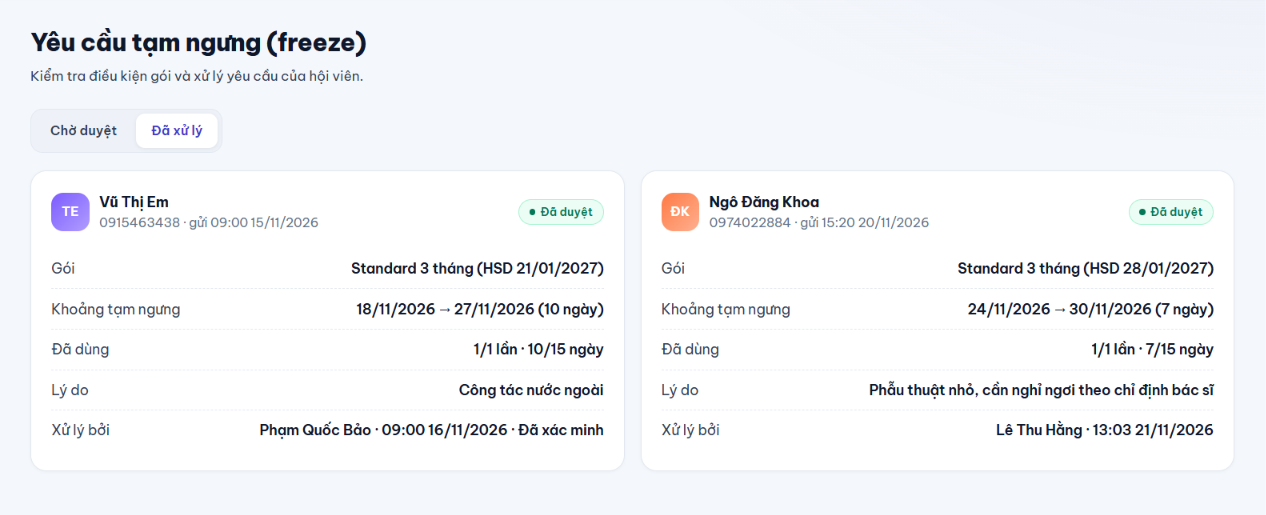
\includegraphics[width=0.92\textwidth]{images/ui_ktpm/daxulyyeyucau.png}
\caption{Giao diện màn hình Nhật ký Yêu cầu Freeze Đã xử lý}
\label{fig:daxulyyeucau}
\end{figure}

\par\medskip\noindent\textbf{Danh sách các thành phần giao diện}\par\smallskip
{\footnotesize
\setlength{\tabcolsep}{2.5pt}
\begin{longtable}{|c|L{2.95cm}|L{1.85cm}|L{2.95cm}|L{2.75cm}|L{1.90cm}|L{2.05cm}|}
\hline
\textbf{STT} & \textbf{Tên} & \textbf{Kiểu} & \textbf{Ý nghĩa} & \textbf{Miền giá trị} & \textbf{Giá trị mặc định} & \textbf{Ghi chú} \\
\hline
\endfirsthead
\hline
\textbf{STT} & \textbf{Tên} & \textbf{Kiểu} & \textbf{Ý nghĩa} & \textbf{Miền giá trị} & \textbf{Giá trị mặc định} & \textbf{Ghi chú} \\
\hline
\endhead
\hline
\endfoot
\hline
\caption{Danh sách các thành phần giao diện -- Màn hình Nhật ký Yêu cầu Freeze Đã xử lý} \\
\endlastfoot
1 & \texttt{Tab\_DaXuLyFreeze} & Tab Group & Chuyển đổi sang xem danh sách hồ sơ Freeze đã hoàn tất thẩm định & \{\texttt{"Chờ duyệt"}, \texttt{"Đã xử lý"}\} & \texttt{"Đã xử lý"} (Active) & Dùng chung thanh tab với màn hình 6.3.7 \\ \hline
2 & \texttt{Card\_NhatKyFreeze} & Card Grid & Lưới thẻ hiển thị thông tin hội viên, gói tập, khoảng nghỉ, lý do và badge kết quả & Bản ghi khác \texttt{pending} trong \texttt{Freeze\_Requests} & Toàn bộ hồ sơ đã xử lý & Chỉ đọc, phục vụ tra cứu kiểm toán \\ \hline
3 & \texttt{Lbl\_HanSauBu} & Label & Hiển thị hạn sử dụng của gói sau khi được cộng bù số ngày tạm ngưng & Ngày hợp lệ (\texttt{dd/MM/yyyy}) & Cập nhật tự động khi duyệt & Ví dụ: tăng từ 21/01 lên 28/01/2027 \\* \hline
4 & \texttt{Lbl\_NhanVienDuyet} & Label & Hiển thị họ tên nhân viên lễ tân xử lý, ngày giờ duyệt và ghi chú kèm theo & Chuỗi thông tin kiểm toán & Theo \texttt{handledBy}, \texttt{handledAt} & Quy rõ trách nhiệm thẩm định \\ \hline
\end{longtable}
}

\par\medskip\noindent\textbf{Danh sách các biến cố}\par\smallskip
{\footnotesize
\setlength{\tabcolsep}{4pt}
\begin{longtable}{|c|L{3.5cm}|L{7.8cm}|L{3.5cm}|}
\hline
\textbf{STT} & \textbf{Điều kiện kích hoạt} & \textbf{Xử lý} & \textbf{Ghi chú} \\
\hline
\endfirsthead
\hline
\textbf{STT} & \textbf{Điều kiện kích hoạt} & \textbf{Xử lý} & \textbf{Ghi chú} \\
\hline
\endhead
\hline
\endfoot
\hline
\caption{Danh sách các biến cố -- Màn hình Nhật ký Yêu cầu Freeze Đã xử lý} \\
\endlastfoot
0 & Khởi động / Chọn tab \textit{Đã xử lý} (\texttt{/staff/freeze}) & Lọc danh sách \texttt{Freeze\_Requests} có trạng thái khác \texttt{pending} (bao gồm \texttt{Approved} và \texttt{Rejected}); truy xuất tên nhân viên từ \texttt{handledBy}, hạn sử dụng đã cập nhật và kết xuất lên \texttt{Card\_NhatKyFreeze}. & Bảo toàn lịch sử kiểm toán không cho chỉnh sửa. \\* \hline
1 & Chuyển tab sang \textit{Chờ duyệt} & Đổi trạng thái tab hiện hành để quay về danh sách hồ sơ đang chờ lễ tân thẩm định tiếp. & Cập nhật tức thời không cần tải lại trang. \\ \hline
\end{longtable}
}

% --- 6.3.9 QUẢN TRỊ DANH MỤC GÓI HỘI VIÊN ---
\subsubsection{Màn hình Quản trị Danh mục Gói Hội viên (Quản trị viên)}
Màn hình \textbf{Quản trị Danh mục Gói Hội viên} (đường dẫn \texttt{/admin/plans}, tab \textit{Gói Hội Viên}) cho phép \textbf{Quản trị viên (Admin)} xem toàn bộ cấu hình các gói hội viên hiện có, thêm mới gói tập, chỉnh sửa thông số kinh doanh hoặc tạm dừng / kích hoạt phát hành gói mà không ảnh hưởng dữ liệu hội viên cũ.

\begin{figure}[H]
\centering
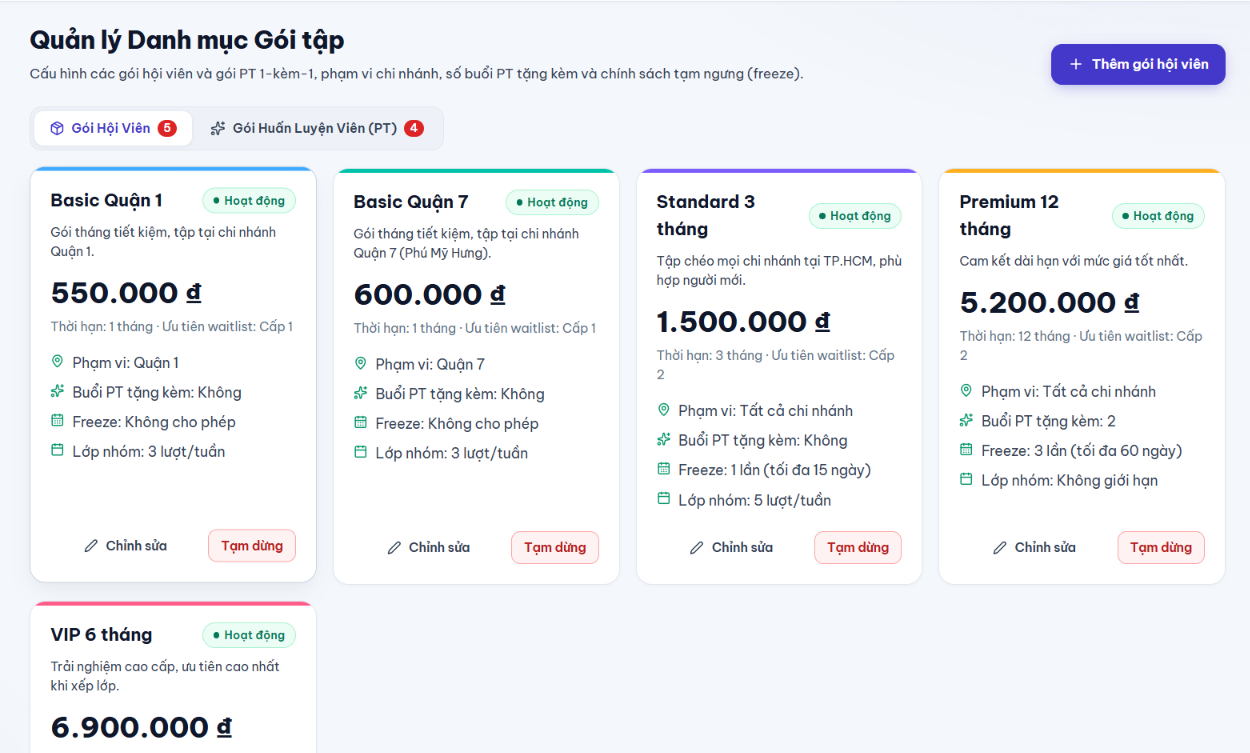
\includegraphics[width=0.92\textwidth]{images/ui_ktpm/QLgoihoivien.png}
\caption{Giao diện màn hình Quản trị Danh mục Gói Hội viên}
\label{fig:qlgoihoivien}
\end{figure}

\par\medskip\noindent\textbf{Danh sách các thành phần giao diện}\par\smallskip
{\footnotesize
\setlength{\tabcolsep}{2.5pt}
\begin{longtable}{|c|L{2.95cm}|L{1.85cm}|L{2.95cm}|L{2.75cm}|L{1.90cm}|L{2.05cm}|}
\hline
\textbf{STT} & \textbf{Tên} & \textbf{Kiểu} & \textbf{Ý nghĩa} & \textbf{Miền giá trị} & \textbf{Giá trị mặc định} & \textbf{Ghi chú} \\
\hline
\endfirsthead
\hline
\textbf{STT} & \textbf{Tên} & \textbf{Kiểu} & \textbf{Ý nghĩa} & \textbf{Miền giá trị} & \textbf{Giá trị mặc định} & \textbf{Ghi chú} \\
\hline
\endhead
\hline
\endfoot
\hline
\caption{Danh sách các thành phần giao diện -- Màn hình Quản trị Danh mục Gói Hội viên} \\
\endlastfoot
1 & \texttt{Tab\_DanhMucGoi} & Tab Group & Chuyển đổi giữa quản trị \textit{Gói Hội Viên} và \textit{Gói Huấn Luyện Viên (PT)} & 2 tab kèm bộ đếm số gói & \texttt{"Gói Hội Viên"} & Thay đổi nhãn nút thêm mới theo tab \\ \hline
2 & \texttt{Btn\_ThemGoiHV} & Button & Mở hộp thoại khai báo cấu hình gói hội viên mới & Kích hoạt & \texttt{"+ Thêm gói hội viên"} & Mở \textit{Hộp thoại Thêm mới Gói Hội viên} \\ \hline
3 & \texttt{Grd\_GoiHVAdmin} & Card Grid & Lưới thẻ hiển thị đầy đủ thông số của từng gói (giá, thời hạn, cấp Waitlist, phạm vi, PT tặng, Freeze, giới hạn lớp) & Toàn bộ bản ghi từ \texttt{Membership\_Plans} & Hiển thị cả gói đang tạm dừng & Thẻ tạm dừng được làm mờ để phân biệt \\ \hline
4 & \texttt{Btn\_SuaGoiHV} & Button & Mở hộp thoại chỉnh sửa thông số gói hội viên tương ứng trên thẻ & Kích hoạt & \texttt{"Chỉnh sửa"} & Nạp sẵn dữ liệu gói được chọn \\* \hline
5 & \texttt{Btn\_TrangThaiGoi} & Button & Chuyển đổi trạng thái kinh doanh của gói giữa \textit{Hoạt động} và \textit{Tạm dừng} & Kích hoạt & \texttt{"Tạm dừng"} / \texttt{"Kích hoạt"} & Không làm mất lịch sử hợp đồng cũ \\ \hline
\end{longtable}
}

\par\medskip\noindent\textbf{Danh sách các biến cố}\par\smallskip
{\footnotesize
\setlength{\tabcolsep}{4pt}
\begin{longtable}{|c|L{3.5cm}|L{7.8cm}|L{3.5cm}|}
\hline
\textbf{STT} & \textbf{Điều kiện kích hoạt} & \textbf{Xử lý} & \textbf{Ghi chú} \\
\hline
\endfirsthead
\hline
\textbf{STT} & \textbf{Điều kiện kích hoạt} & \textbf{Xử lý} & \textbf{Ghi chú} \\
\hline
\endhead
\hline
\endfoot
\hline
\caption{Danh sách các biến cố -- Màn hình Quản trị Danh mục Gói Hội viên} \\
\endlastfoot
0 & Khởi động màn hình (\texttt{/admin/plans}) & Tải toàn bộ danh mục gói hội viên từ \texttt{Membership\_Plans} (gồm gói hội viên và gói PT phân loại theo \texttt{Plan\_Type}); mặc định mở tab \textit{Gói Hội Viên} và hiển thị lưới thẻ \texttt{Grd\_GoiHVAdmin}. & Cập nhật số lượng trên tiêu đề 2 tab. \\ \hline
1 & Nhấn nút \texttt{Btn\_ThemGoiHV} (\textit{+ Thêm gói hội viên}) & Mở \textit{Hộp thoại Thêm mới Gói Hội viên} ở chế độ tạo mới với các giá trị khởi tạo mặc định. & Cho phép khai báo gói mới. \\ \hline
2 & Nhấn nút \texttt{Btn\_SuaGoiHV} (\textit{Chỉnh sửa}) trên một thẻ gói & Truyền đối tượng gói tập hiện tại sang \textit{Hộp thoại Chỉnh sửa Gói Hội viên} để cập nhật thông số. & Tự động đổ sẵn toàn bộ giá trị hiện có. \\ \hline
3 & Nhấn nút \texttt{Btn\_TrangThaiGoi} (\textit{Tạm dừng} / \textit{Kích hoạt}) & Đảo cờ trạng thái \texttt{active} của gói trong \texttt{Membership\_Plans}; hiển thị Toast xác nhận và cập nhật giao diện thẻ (ẩn khỏi trang mua mới của hội viên nếu tạm dừng). & Giữ nguyên quyền lợi hội viên đã mua trước đó. \\* \hline
4 & Chọn tab \textit{Gói Huấn Luyện Viên (PT)} trên \texttt{Tab\_DanhMucGoi} & Chuyển vùng hiển thị sang danh sách thẻ gói PT và đổi nút hành động chính thành \texttt{"+ Thêm gói PT"}. & Điều hướng liền mạch trong cùng màn hình. \\ \hline
\end{longtable}
}

% --- 6.3.10 HỘP THOẠI THÊM MỚI GÓI HỘI VIÊN ---
\subsubsection{Hộp thoại Thêm mới Gói Hội viên (Quản trị viên)}
\textbf{Hộp thoại Thêm mới Gói Hội viên} cho phép \textbf{Quản trị viên} thiết kế biểu mẫu hai cột để khai báo gói hội viên mới với đầy đủ quy tắc kinh doanh: đơn giá, thời hạn, mức ưu tiên Waitlist, số buổi PT tặng kèm, giới hạn lớp/tháng, chính sách Freeze, màu đại diện và phạm vi chi nhánh.

\begin{figure}[H]
\centering
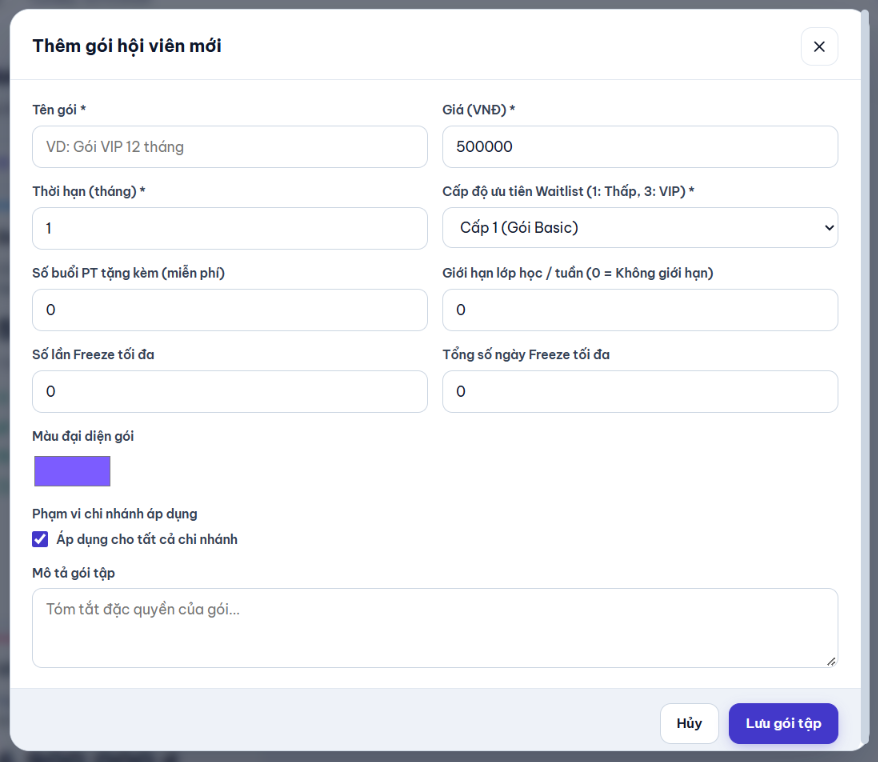
\includegraphics[width=0.58\textwidth]{images/ui_ktpm/themmoigoihoivien.png}
\caption{Giao diện Hộp thoại Thêm mới Gói Hội viên}
\label{fig:themmoigoihoivien}
\end{figure}

\par\medskip\noindent\textbf{Danh sách các thành phần giao diện}\par\smallskip
{\footnotesize
\setlength{\tabcolsep}{2.5pt}
\begin{longtable}{|c|L{2.95cm}|L{1.85cm}|L{2.95cm}|L{2.75cm}|L{1.90cm}|L{2.05cm}|}
\hline
\textbf{STT} & \textbf{Tên} & \textbf{Kiểu} & \textbf{Ý nghĩa} & \textbf{Miền giá trị} & \textbf{Giá trị mặc định} & \textbf{Ghi chú} \\
\hline
\endfirsthead
\hline
\textbf{STT} & \textbf{Tên} & \textbf{Kiểu} & \textbf{Ý nghĩa} & \textbf{Miền giá trị} & \textbf{Giá trị mặc định} & \textbf{Ghi chú} \\
\hline
\endhead
\hline
\endfoot
\hline
\caption{Danh sách các thành phần giao diện -- Hộp thoại Thêm mới Gói Hội viên} \\
\endlastfoot
1 & \texttt{Txt\_TenGoiHV} & Textbox & Tên thương mại của gói hội viên & Chuỗi ký tự không rỗng & Rỗng & Bắt buộc nhập \\ \hline
2 & \texttt{Num\_GiaGoiHV} & NumberInput & Đơn giá bán niêm yết của gói & Số nguyên $> 0$ (VNĐ) & \texttt{500000} & Bước nhảy $50.000$ đ \\ \hline
3 & \texttt{Num\_ThoiHanThang} & NumberInput & Số tháng hiệu lực của gói tập & Số nguyên $\ge 1$ & $1$ tháng & Bắt buộc \\ \hline
4 & \texttt{Cbo\_UuTienWL} & ComboBox & Cấp độ ưu tiên khi xét danh sách chờ Waitlist & \{\texttt{Cấp 1}, \texttt{Cấp 2}, \texttt{Cấp 3}\} & \texttt{Cấp 1 (Gói Basic)} & Cấp 3 là ưu tiên VIP \\ \hline
5 & \texttt{Num\_BuoiPTTang} & NumberInput & Số buổi PT 1-kèm-1 tặng kèm miễn phí & Số nguyên $\ge 0$ & $0$ buổi & $0$ nếu không tặng kèm \\ \hline
6 & \texttt{Num\_GioiHanLop} & NumberInput & Giới hạn số buổi lớp nhóm đặt tối đa mỗi tháng (\texttt{Max\_Bookings\_Per\_Month}) & Số nguyên $\ge 0$ & $0$ (Không giới hạn) & $0$ nghĩa là không giới hạn \\ \hline
7 & \texttt{Num\_SoLanFreeze} & NumberInput & Số lần tối đa hội viên được gửi yêu cầu Freeze & Số nguyên $\ge 0$ & $0$ lần & $0$ nếu không hỗ trợ Freeze \\ \hline
8 & \texttt{Num\_SoNgayFreeze} & NumberInput & Tổng số ngày tạm ngưng tối đa cho phép của gói & Số nguyên $\ge 0$ & $0$ ngày & Đối soát cùng số lần Freeze \\ \hline
9 & \texttt{Clr\_MauDaiDien} & ColorPicker & Chọn màu nhận diện cho thẻ gói tập & Mã màu Hex & \texttt{\#7c5cff} & Hiển thị trên dải màu thẻ \\ \hline
10 & \texttt{Chk\_TatCaCNHV} & Checkbox & Thiết lập gói áp dụng trên toàn hệ thống hay theo chi nhánh lẻ & \{\texttt{True}, \texttt{False}\} & \texttt{True} (Đã chọn) & Bỏ chọn sẽ mở danh sách chi nhánh \\ \hline
11 & \texttt{Txt\_MoTaGoiHV} & TextArea & Nhập mô tả tóm tắt quyền lợi nổi bật của gói & Văn bản nhiều dòng & Rỗng & Hiển thị dưới tên gói \\ \hline
12 & \texttt{Btn\_HuyThemHV} & Button & Hủy thao tác và đóng hộp thoại thêm mới & Kích hoạt & \texttt{"Hủy"} & Không lưu thay đổi \\* \hline
13 & \texttt{Btn\_LuuGoiHV} & Button & Kiểm tra dữ liệu hợp lệ và lưu gói hội viên mới vào CSDL & Kích hoạt & \texttt{"Lưu gói tập"} & Nút hành động chính \\ \hline
\end{longtable}
}

\par\medskip\noindent\textbf{Danh sách các biến cố}\par\smallskip
{\footnotesize
\setlength{\tabcolsep}{4pt}
\begin{longtable}{|c|L{3.5cm}|L{7.8cm}|L{3.5cm}|}
\hline
\textbf{STT} & \textbf{Điều kiện kích hoạt} & \textbf{Xử lý} & \textbf{Ghi chú} \\
\hline
\endfirsthead
\hline
\textbf{STT} & \textbf{Điều kiện kích hoạt} & \textbf{Xử lý} & \textbf{Ghi chú} \\
\hline
\endhead
\hline
\endfoot
\hline
\caption{Danh sách các biến cố -- Hộp thoại Thêm mới Gói Hội viên} \\
\endlastfoot
0 & Mở hộp thoại Thêm mới Gói Hội viên & Khởi tạo các ô nhập liệu với giá trị mặc định (thời hạn $1$ tháng, giá $500.000$ đ, ưu tiên Cấp $1$, áp dụng tất cả chi nhánh) và ẩn vùng chọn chi nhánh lẻ. & Sẵn sàng tiếp nhận cấu hình mới. \\ \hline
1 & Bật hoặc tắt checkbox \texttt{Chk\_TatCaCNHV} & Nếu bỏ chọn, giao diện mở rộng danh sách các chip chi nhánh để Quản trị viên chọn từng cơ sở áp dụng (\texttt{Plan\_Branches}); nếu chọn lại, gán phạm vi toàn chuỗi (\texttt{all}). & Đảm bảo mỗi gói luôn có phạm vi xác định. \\ \hline
2 & Nhấn nút \texttt{Btn\_LuuGoiHV} (\textit{Lưu gói tập}) & Kiểm tra tên gói không rỗng, giá $> 0$ và thời hạn $\ge 1$; nếu hợp lệ thì sinh bản ghi mới vào \texttt{Membership\_Plans} (trạng thái \texttt{active = true}), hiển thị Toast \textit{``Đã thêm gói hội viên mới''}, đóng modal và làm mới lưới. & Nếu thiếu tên gói, báo lỗi yêu cầu nhập tên. \\* \hline
3 & Nhấn nút \texttt{Btn\_HuyThemHV} (\textit{Hủy}) hoặc \texttt{$\times$} & Đóng hộp thoại và hủy bỏ toàn bộ thông tin đang nhập trên biểu mẫu. & Không làm thay đổi danh mục gói hiện có. \\ \hline
\end{longtable}
}

% --- 6.3.11 HỘP THOẠI CHỈNH SỬA GÓI HỘI VIÊN ---
\subsubsection{Hộp thoại Chỉnh sửa Gói Hội viên (Quản trị viên)}
\textbf{Hộp thoại Chỉnh sửa Gói Hội viên} nạp sẵn toàn bộ thông số cấu hình hiện hành của gói được chọn, cho phép \textbf{Quản trị viên} điều chỉnh giá bán, thời hạn, hạn mức Freeze, mô tả hoặc chuyển đổi phạm vi áp dụng sang từng chi nhánh cụ thể qua nhóm nút chọn đa chi nhánh.

\begin{figure}[H]
\centering
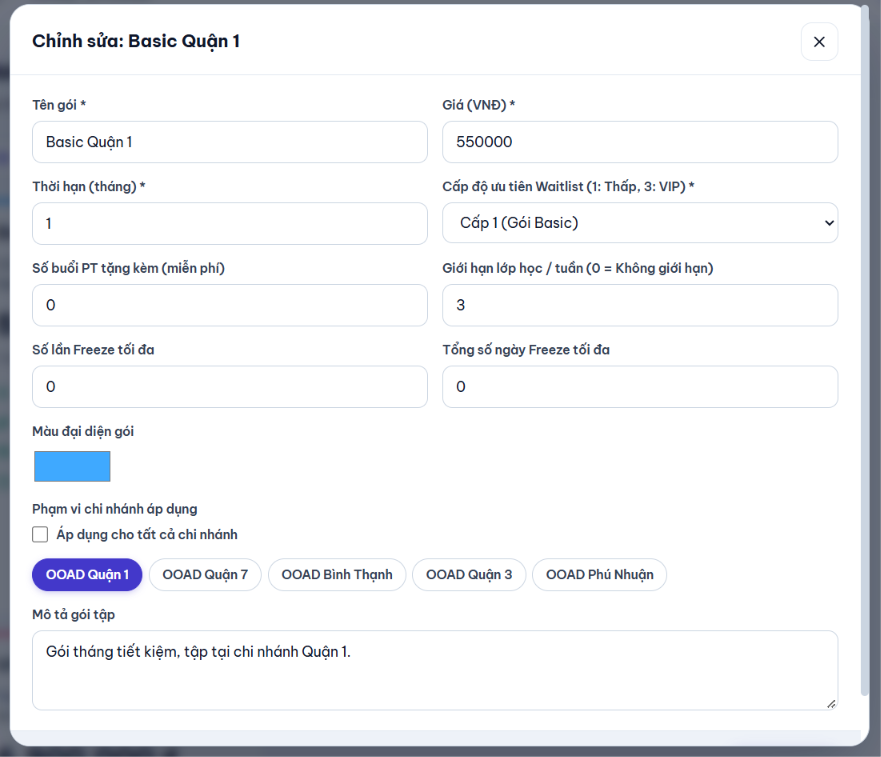
\includegraphics[width=0.58\textwidth]{images/ui_ktpm/chinhsuagoihoivien.png}
\caption{Giao diện Hộp thoại Chỉnh sửa Gói Hội viên}
\label{fig:chinhsuagoihoivien}
\end{figure}

\par\medskip\noindent\textbf{Danh sách các thành phần giao diện}\par\smallskip
{\footnotesize
\setlength{\tabcolsep}{2.5pt}
\begin{longtable}{|c|L{2.95cm}|L{1.85cm}|L{2.95cm}|L{2.75cm}|L{1.90cm}|L{2.05cm}|}
\hline
\textbf{STT} & \textbf{Tên} & \textbf{Kiểu} & \textbf{Ý nghĩa} & \textbf{Miền giá trị} & \textbf{Giá trị mặc định} & \textbf{Ghi chú} \\
\hline
\endfirsthead
\hline
\textbf{STT} & \textbf{Tên} & \textbf{Kiểu} & \textbf{Ý nghĩa} & \textbf{Miền giá trị} & \textbf{Giá trị mặc định} & \textbf{Ghi chú} \\
\hline
\endhead
\hline
\endfoot
\hline
\caption{Danh sách các thành phần giao diện -- Hộp thoại Chỉnh sửa Gói Hội viên} \\
\endlastfoot
1 & \texttt{Txt\_SuaTenGoiHV} & Textbox & Chỉnh sửa tên gói hội viên đang chọn & Chuỗi ký tự không rỗng & Giá trị gói hiện tại & Ví dụ: \texttt{"Basic Quận 1"} \\ \hline
2 & \texttt{Num\_SuaGiaGoiHV} & NumberInput & Điều chỉnh giá niêm yết mới của gói & Số nguyên $> 0$ & Giá hiện tại của gói & Không ảnh hưởng hợp đồng đã bán \\ \hline
3 & \texttt{Chk\_\hspace{0pt}SuaTatCaCN} & Checkbox & Bật/tắt chế độ áp dụng toàn bộ chi nhánh & \{\texttt{True}, \texttt{False}\} & Theo \texttt{branchScope} của gói & Khi bỏ chọn sẽ hiện \texttt{Chip\_\hspace{0pt}ChiNhanhHV} \\ \hline
4 & \texttt{Chip\_ChiNhanhHV} & Chip Button & Nhóm nút đa chọn các chi nhánh áp dụng lẻ & Danh sách từ \texttt{Branches} & Các chi nhánh đã gán & Bật/tắt viền tím nổi bật \\ \hline
5 & \texttt{Txt\_SuaMoTaHV} & TextArea & Cập nhật văn bản mô tả quyền lợi gói tập & Văn bản nhiều dòng & Mô tả hiện tại & Hỗ trợ cập nhật nội dung tiếp thị \\* \hline
6 & \texttt{Btn\_LuuSuaHV} & Button & Lưu các thay đổi cấu hình gói hội viên vào CSDL & Kích hoạt & \texttt{"Lưu gói tập"} & Đi kèm nút \texttt{"Hủy"} \\ \hline
\end{longtable}
}

\par\medskip\noindent\textbf{Danh sách các biến cố}\par\smallskip
{\footnotesize
\setlength{\tabcolsep}{4pt}
\begin{longtable}{|c|L{3.5cm}|L{7.8cm}|L{3.5cm}|}
\hline
\textbf{STT} & \textbf{Điều kiện kích hoạt} & \textbf{Xử lý} & \textbf{Ghi chú} \\
\hline
\endfirsthead
\hline
\textbf{STT} & \textbf{Điều kiện kích hoạt} & \textbf{Xử lý} & \textbf{Ghi chú} \\
\hline
\endhead
\hline
\endfoot
\hline
\caption{Danh sách các biến cố -- Hộp thoại Chỉnh sửa Gói Hội viên} \\
\endlastfoot
0 & Mở hộp thoại Chỉnh sửa Gói Hội viên & Nạp toàn bộ thông tin gói đang chọn (tên, giá, thời hạn, cấp Waitlist, Freeze, màu sắc, mô tả) vào biểu mẫu; nếu gói giới hạn chi nhánh thì bỏ chọn \texttt{Chk\_SuaTatCaCN} và tô sáng các chip chi nhánh tương ứng. & Tiết kiệm thao tác nhập lại dữ liệu. \\ \hline
1 & Bấm bật/tắt chip trên \texttt{Chip\_ChiNhanhHV} & Thêm hoặc loại bỏ mã chi nhánh khỏi mảng chi nhánh áp dụng của gói và cập nhật màu viền nổi bật trên chip được chọn. & Cho phép gán linh hoạt 1 hoặc nhiều chi nhánh. \\ \hline
2 & Nhấn nút \texttt{Btn\_LuuSuaHV} (\textit{Lưu gói tập}) & Kiểm tra tính hợp lệ của tên gói và các trường số; cập nhật bản ghi trong \texttt{Membership\_Plans} và liên kết \texttt{Plan\_Branches}, hiển thị Toast \textit{``Đã cập nhật gói hội viên''}, đóng modal và làm mới lưới. & Áp dụng ngay cho giao dịch mua/gia hạn mới. \\* \hline
3 & Nhấn nút \textit{Hủy} hoặc \texttt{$\times$} & Đóng hộp thoại chỉnh sửa mà không ghi đè dữ liệu gốc trong CSDL. & An toàn khi người dùng hủy thao tác. \\ \hline
\end{longtable}
}

% --- 6.3.12 QUẢN TRỊ DANH MỤC GÓI HUẤN LUYỆN VIÊN ---
\subsubsection{Màn hình Quản trị Danh mục Gói Huấn luyện viên (Quản trị viên)}
Màn hình \textbf{Quản trị Danh mục Gói Huấn luyện viên} (đường dẫn \texttt{/admin/plans}, tab \textit{Gói Huấn Luyện Viên (PT)}) giúp \textbf{Quản trị viên} quản lý tập trung các gói tập 1-kèm-1, tự động tính đơn giá trung bình mỗi buổi, phạm vi chi nhánh và cung cấp các thao tác thêm mới, chỉnh sửa hoặc tạm dừng kinh doanh gói PT.

\begin{figure}[H]
\centering
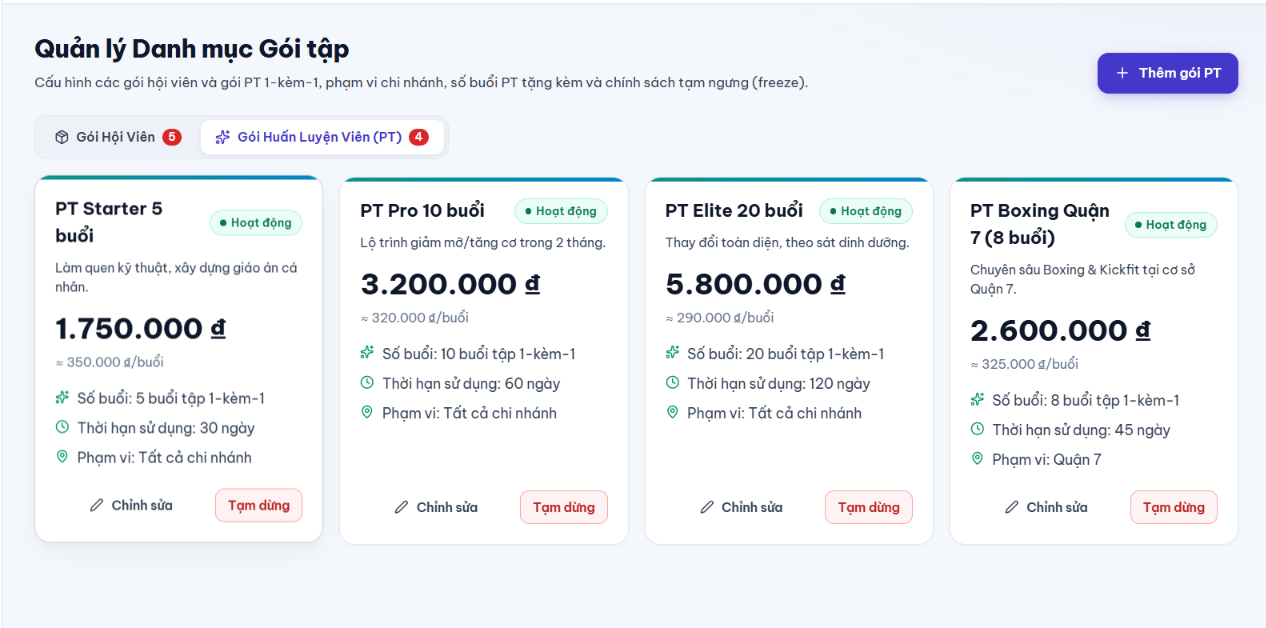
\includegraphics[width=0.92\textwidth]{images/ui_ktpm/QlgoiPT.png}
\caption{Giao diện màn hình Quản trị Danh mục Gói Huấn luyện viên (PT)}
\label{fig:qlgoipt}
\end{figure}

\par\medskip\noindent\textbf{Danh sách các thành phần giao diện}\par\smallskip
{\footnotesize
\setlength{\tabcolsep}{2.5pt}
\begin{longtable}{|c|L{2.95cm}|L{1.85cm}|L{2.95cm}|L{2.75cm}|L{1.90cm}|L{2.05cm}|}
\hline
\textbf{STT} & \textbf{Tên} & \textbf{Kiểu} & \textbf{Ý nghĩa} & \textbf{Miền giá trị} & \textbf{Giá trị mặc định} & \textbf{Ghi chú} \\
\hline
\endfirsthead
\hline
\textbf{STT} & \textbf{Tên} & \textbf{Kiểu} & \textbf{Ý nghĩa} & \textbf{Miền giá trị} & \textbf{Giá trị mặc định} & \textbf{Ghi chú} \\
\hline
\endhead
\hline
\endfoot
\hline
\caption{Danh sách các thành phần giao diện -- Màn hình Quản trị Danh mục Gói PT} \\
\endlastfoot
1 & \texttt{Btn\_ThemGoiPT} & Button & Mở hộp thoại khai báo một gói PT 1-kèm-1 mới & Kích hoạt & \texttt{"+ Thêm gói PT"} & Đổi nhãn từ nút thêm gói hội viên \\ \hline
2 & \texttt{Grd\_GoiPTAdmin} & Card Grid & Lưới thẻ hiển thị thông tin từng gói PT (tên, trạng thái, giá, đơn giá/buổi, số buổi, hạn ngày, phạm vi) & Danh sách bản ghi từ \texttt{Membership\_Plans} (\texttt{Plan\_Type = 'PT'}) & Toàn bộ gói PT hiện có & Có dải màu nhận diện phía trên thẻ \\ \hline
3 & \texttt{Btn\_SuaGoiPT} & Button & Mở hộp thoại chỉnh sửa thông số gói PT tương ứng & Kích hoạt & \texttt{"Chỉnh sửa"} & Nạp dữ liệu gói vào form sửa \\* \hline
4 & \texttt{Btn\_TrangThaiPT} & Button & Đổi trạng thái phát hành của gói PT giữa \textit{Hoạt động} và \textit{Tạm dừng} & Kích hoạt & \texttt{"Tạm dừng"} / \texttt{"Kích hoạt"} & Ngừng bán mới nhưng giữ gói đã mua \\ \hline
\end{longtable}
}

\par\medskip\noindent\textbf{Danh sách các biến cố}\par\smallskip
{\footnotesize
\setlength{\tabcolsep}{4pt}
\begin{longtable}{|c|L{3.5cm}|L{7.8cm}|L{3.5cm}|}
\hline
\textbf{STT} & \textbf{Điều kiện kích hoạt} & \textbf{Xử lý} & \textbf{Ghi chú} \\
\hline
\endfirsthead
\hline
\textbf{STT} & \textbf{Điều kiện kích hoạt} & \textbf{Xử lý} & \textbf{Ghi chú} \\
\hline
\endhead
\hline
\endfoot
\hline
\caption{Danh sách các biến cố -- Màn hình Quản trị Danh mục Gói PT} \\
\endlastfoot
0 & Khởi động / Chọn tab \textit{Gói Huấn Luyện Viên (PT)} (\texttt{/admin/plans}) & Tải danh sách gói PT từ \texttt{Membership\_Plans} (\texttt{Plan\_Type = 'PT'}), tính đơn giá trung bình mỗi buổi (\texttt{price / sessions}), đổi nhãn nút hành động sang \texttt{"+ Thêm gói PT"} và hiển thị lưới thẻ \texttt{Grd\_GoiPTAdmin}. & Phân biệt trực quan với tab Gói Hội Viên. \\ \hline
1 & Nhấn nút \texttt{Btn\_ThemGoiPT} (\textit{+ Thêm gói PT}) & Mở \textit{Hộp thoại Thêm mới Gói PT} với form trống và thông số mặc định. & Khởi tạo gói đào tạo mới. \\ \hline
2 & Nhấn nút \texttt{Btn\_SuaGoiPT} (\textit{Chỉnh sửa}) trên thẻ gói PT & Truyền thông số gói PT được chọn sang \textit{Hộp thoại Chỉnh sửa Gói PT} để cập nhật. & Hỗ trợ cập nhật nhanh giá và số buổi. \\* \hline
3 & Nhấn nút \texttt{Btn\_TrangThaiPT} (\textit{Tạm dừng} / \textit{Kích hoạt}) & Cập nhật cờ trạng thái \texttt{active} của gói PT trong CSDL; hiển thị Toast thông báo và làm mới thẻ trên lưới. & Không ảnh hưởng buổi PT hội viên đã mua. \\ \hline
\end{longtable}
}

% --- 6.3.13 HỘP THOẠI THÊM MỚI GÓI PT ---
\subsubsection{Hộp thoại Thêm mới Gói PT (Quản trị viên)}
\textbf{Hộp thoại Thêm mới Gói PT} cung cấp biểu mẫu tinh giản giúp \textbf{Quản trị viên} thiết lập nhanh gói huấn luyện viên cá nhân mới với các trường đặc thù: tên gói PT, tổng số buổi tập, thời hạn sử dụng (ngày), giá tiền, phạm vi chi nhánh và mô tả mục tiêu tập luyện.

\begin{figure}[H]
\centering
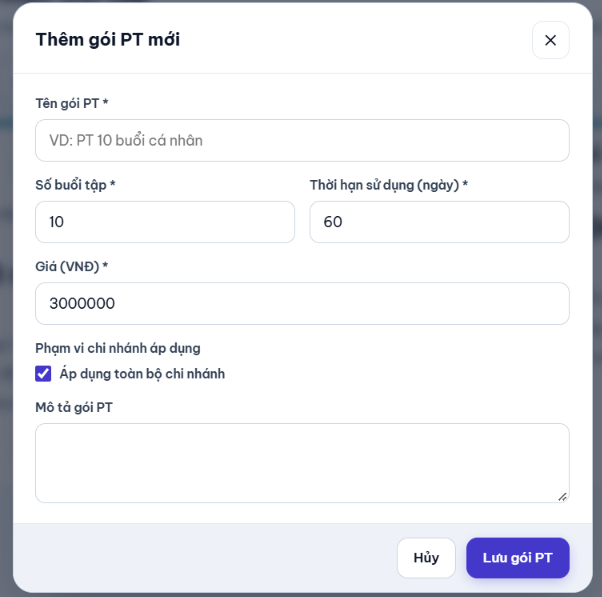
\includegraphics[width=0.58\textwidth]{images/ui_ktpm/themmoipt.png}
\caption{Giao diện Hộp thoại Thêm mới Gói PT}
\label{fig:themmoipt}
\end{figure}

\par\medskip\noindent\textbf{Danh sách các thành phần giao diện}\par\smallskip
{\footnotesize
\setlength{\tabcolsep}{2.5pt}
\begin{longtable}{|c|L{2.95cm}|L{1.85cm}|L{2.95cm}|L{2.75cm}|L{1.90cm}|L{2.05cm}|}
\hline
\textbf{STT} & \textbf{Tên} & \textbf{Kiểu} & \textbf{Ý nghĩa} & \textbf{Miền giá trị} & \textbf{Giá trị mặc định} & \textbf{Ghi chú} \\
\hline
\endfirsthead
\hline
\textbf{STT} & \textbf{Tên} & \textbf{Kiểu} & \textbf{Ý nghĩa} & \textbf{Miền giá trị} & \textbf{Giá trị mặc định} & \textbf{Ghi chú} \\
\hline
\endhead
\hline
\endfoot
\hline
\caption{Danh sách các thành phần giao diện -- Hộp thoại Thêm mới Gói PT} \\
\endlastfoot
1 & \texttt{Txt\_TenGoiPT} & Textbox & Nhập tên thương mại của gói PT 1-kèm-1 & Chuỗi ký tự không rỗng & Rỗng & Bắt buộc nhập \\ \hline
2 & \texttt{Num\_SoBuoiPT} & NumberInput & Tổng số buổi tập 1-kèm-1 trong gói & Số nguyên $\ge 1$ & $10$ buổi & Dùng để tính đơn giá mỗi buổi \\ \hline
3 & \texttt{Num\_ThoiHanPT} & NumberInput & Thời hạn sử dụng gói tính theo ngày & Số nguyên $\ge 1$ & $60$ ngày & Kể từ ngày kích hoạt \\ \hline
4 & \texttt{Num\_GiaGoiPT} & NumberInput & Tổng chi phí trọn gói tính theo VNĐ & Số nguyên $> 0$ & \texttt{3000000} & Đơn vị VNĐ \\ \hline
5 & \texttt{Chk\_TatCaCNPT} & Checkbox & Phạm vi áp dụng toàn chuỗi hoặc chọn chi nhánh lẻ & \{\texttt{True}, \texttt{False}\} & \texttt{True} (Đã chọn) & Bỏ chọn để hiện chip chi nhánh \\ \hline
6 & \texttt{Txt\_MoTaGoiPT} & TextArea & Định hướng giáo án và mục tiêu tập luyện của gói & Văn bản nhiều dòng & Rỗng & Tùy chọn nhập \\* \hline
7 & \texttt{Btn\_LuuGoiPT} & Button & Kiểm tra hợp lệ và lưu cấu hình gói PT mới vào CSDL & Kích hoạt & \texttt{"Lưu gói PT"} & Đi kèm nút \texttt{"Hủy"} \\ \hline
\end{longtable}
}

\par\medskip\noindent\textbf{Danh sách các biến cố}\par\smallskip
{\footnotesize
\setlength{\tabcolsep}{4pt}
\begin{longtable}{|c|L{3.5cm}|L{7.8cm}|L{3.5cm}|}
\hline
\textbf{STT} & \textbf{Điều kiện kích hoạt} & \textbf{Xử lý} & \textbf{Ghi chú} \\
\hline
\endfirsthead
\hline
\textbf{STT} & \textbf{Điều kiện kích hoạt} & \textbf{Xử lý} & \textbf{Ghi chú} \\
\hline
\endhead
\hline
\endfoot
\hline
\caption{Danh sách các biến cố -- Hộp thoại Thêm mới Gói PT} \\
\endlastfoot
0 & Mở hộp thoại Thêm mới Gói PT & Khởi tạo các giá trị mặc định (10 buổi, 60 ngày, 3.000.000 đ, áp dụng toàn bộ chi nhánh) và đặt tiêu điểm vào ô \texttt{Txt\_TenGoiPT}. & Chuẩn bị biểu mẫu khai báo nhanh. \\ \hline
1 & Bật hoặc tắt \texttt{Chk\_TatCaCNPT} & Chuyển đổi phạm vi áp dụng giữa toàn bộ hệ thống và danh sách các chi nhánh được chọn thủ công. & Tương tự cấu hình gói hội viên. \\ \hline
2 & Nhấn nút \texttt{Btn\_LuuGoiPT} (\textit{Lưu gói PT}) & Kiểm tra tên gói không rỗng, số buổi $\ge 1$, thời hạn $\ge 1$ và giá $> 0$; lưu bản ghi mới vào \texttt{Membership\_Plans} (\texttt{Plan\_Type = 'PT'}), hiển thị Toast \textit{``Đã thêm gói PT mới''}, đóng modal và cập nhật lưới thẻ. & Báo lỗi nếu bỏ trống tên gói PT. \\* \hline
3 & Nhấn nút \textit{Hủy} hoặc \texttt{$\times$} & Đóng hộp thoại và không lưu dữ liệu vừa nhập. & Trả về danh mục gói PT. \\ \hline
\end{longtable}
}

% --- 6.3.14 HỘP THOẠI CHỈNH SỬA GÓI PT ---
\subsubsection{Hộp thoại Chỉnh sửa Gói PT (Quản trị viên)}
\textbf{Hộp thoại Chỉnh sửa Gói PT} cho phép \textbf{Quản trị viên} cập nhật linh hoạt tên gói, số buổi đào tạo, số ngày hiệu lực, đơn giá, phạm vi chi nhánh và mô tả giáo án cho các gói PT đang lưu hành trên hệ thống.

\begin{figure}[H]
\centering
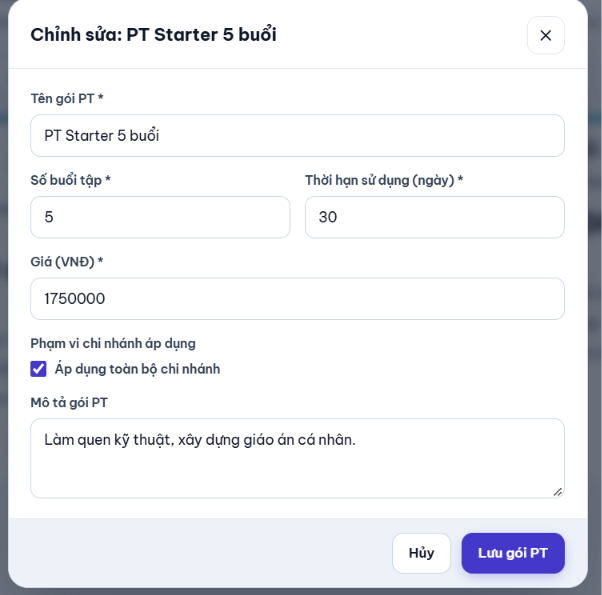
\includegraphics[width=0.58\textwidth]{images/ui_ktpm/chinhsuapt.png}
\caption{Giao diện Hộp thoại Chỉnh sửa Gói PT}
\label{fig:chinhsuapt}
\end{figure}

\par\medskip\noindent\textbf{Danh sách các thành phần giao diện}\par\smallskip
{\footnotesize
\setlength{\tabcolsep}{2.5pt}
\begin{longtable}{|c|L{2.95cm}|L{1.85cm}|L{2.95cm}|L{2.75cm}|L{1.90cm}|L{2.05cm}|}
\hline
\textbf{STT} & \textbf{Tên} & \textbf{Kiểu} & \textbf{Ý nghĩa} & \textbf{Miền giá trị} & \textbf{Giá trị mặc định} & \textbf{Ghi chú} \\
\hline
\endfirsthead
\hline
\textbf{STT} & \textbf{Tên} & \textbf{Kiểu} & \textbf{Ý nghĩa} & \textbf{Miền giá trị} & \textbf{Giá trị mặc định} & \textbf{Ghi chú} \\
\hline
\endhead
\hline
\endfoot
\hline
\caption{Danh sách các thành phần giao diện -- Hộp thoại Chỉnh sửa Gói PT} \\
\endlastfoot
1 & \texttt{Txt\_SuaTenPT} & Textbox & Chỉnh sửa tên gói PT đang chọn & Chuỗi ký tự không rỗng & Giá trị gói hiện tại & Ví dụ: \texttt{"PT Starter 5 buổi"} \\ \hline
2 & \texttt{Num\_SuaSoBuoi} & NumberInput & Điều chỉnh số buổi tập 1-kèm-1 của gói & Số nguyên $\ge 1$ & Số buổi hiện tại & Cập nhật lại đơn giá trung bình \\ \hline
3 & \texttt{Num\_SuaThoiHan} & NumberInput & Cập nhật thời hạn sử dụng tính theo ngày & Số nguyên $\ge 1$ & Số ngày hiện tại & Áp dụng cho giao dịch mua mới \\ \hline
4 & \texttt{Num\_SuaGiaPT} & NumberInput & Điều chỉnh tổng chi phí của gói PT & Số nguyên $> 0$ & Giá hiện tại & Đơn vị VNĐ \\ \hline
5 & \texttt{Txt\_SuaMoTaPT} & TextArea & Chỉnh sửa nội dung mô tả mục tiêu tập luyện & Văn bản nhiều dòng & Mô tả hiện tại & Tùy chọn cập nhật \\* \hline
6 & \texttt{Btn\_LuuSuaPT} & Button & Kiểm tra tính toàn vẹn và lưu thay đổi vào CSDL & Kích hoạt & \texttt{"Lưu gói PT"} & Đi kèm nút \texttt{"Hủy"} \\ \hline
\end{longtable}
}

\par\medskip\noindent\textbf{Danh sách các biến cố}\par\smallskip
{\footnotesize
\setlength{\tabcolsep}{4pt}
\begin{longtable}{|c|L{3.5cm}|L{7.8cm}|L{3.5cm}|}
\hline
\textbf{STT} & \textbf{Điều kiện kích hoạt} & \textbf{Xử lý} & \textbf{Ghi chú} \\
\hline
\endfirsthead
\hline
\textbf{STT} & \textbf{Điều kiện kích hoạt} & \textbf{Xử lý} & \textbf{Ghi chú} \\
\hline
\endhead
\hline
\endfoot
\hline
\caption{Danh sách các biến cố -- Hộp thoại Chỉnh sửa Gói PT} \\
\endlastfoot
0 & Mở hộp thoại Chỉnh sửa Gói PT & Nạp đầy đủ thông số hiện hành của gói PT được chọn (tên, số buổi, thời hạn ngày, giá, phạm vi chi nhánh và mô tả) lên biểu mẫu chỉnh sửa. & Hiển thị tiêu đề \textit{``Chỉnh sửa: <Tên gói>''}. \\ \hline
1 & Thay đổi các trường thông tin hoặc phạm vi chi nhánh & Cập nhật giá trị tạm thời trên trạng thái biểu mẫu, cho phép bật/tắt áp dụng toàn chuỗi hoặc chọn lại danh sách chi nhánh. & Hỗ trợ xem trước thay đổi trước khi lưu. \\ \hline
2 & Nhấn nút \texttt{Btn\_LuuSuaPT} (\textit{Lưu gói PT}) & Kiểm tra tên gói và các trường số hợp lệ; cập nhật bản ghi trong \texttt{Membership\_Plans} (\texttt{Plan\_Type = 'PT'}), hiển thị Toast \textit{``Đã cập nhật gói PT''}, đóng modal và tính lại đơn giá/buổi trên thẻ. & Các gói hội viên đã mua trước đó không bị đổi giá. \\* \hline
3 & Nhấn nút \textit{Hủy} hoặc \texttt{$\times$} & Đóng hộp thoại và giữ nguyên dữ liệu gốc của gói PT. & An toàn khi hủy cập nhật. \\ \hline
\end{longtable}
}

% --- 6.3.15 MA TRẬN PHÂN QUYỀN PHÂN HỆ GÓI TẬP ---
\subsubsection{Bảng Ma trận phân quyền phân hệ Gói tập theo 3 nhóm tác nhân}
Bảng dưới đây tổng hợp quyền truy cập và thao tác của 3 nhóm tác nhân chính (\textbf{Hội viên}, \textbf{Nhân viên Lễ tân}, \textbf{Quản trị viên}) trên toàn bộ các màn hình và hộp thoại thuộc phân hệ Gói tập, Thanh toán \& Bảo lưu (Freeze):

\begin{table}[H]
\centering
{\footnotesize
\setlength{\tabcolsep}{4pt}
\begin{tabularx}{\textwidth}{|L{3.3cm}|Y|C{1.7cm}|C{1.7cm}|C{1.9cm}|}
\hline
\textbf{Nhóm nghiệp vụ} & \textbf{Chi tiết màn hình / Chức năng} & \textbf{Hội viên} & \textbf{Lễ tân} & \textbf{Quản trị viên} \\ \hline
\multirow{3}{3.3cm}{\textbf{Xem \& Quản lý gói}} & Màn hình Tổng quan Gói tập của tôi (\texttt{/member/memberships}) & $\checkmark$ & & \\ \cline{2-5}
 & Màn hình Danh mục Gia hạn / Mua gói Hội viên & $\checkmark$ & & \\ \cline{2-5}
 & Màn hình Danh mục Gói PT 1-kèm-1 & $\checkmark$ & & \\ \hline
\multirow{2}{3.3cm}{\textbf{Thanh toán \& Lịch sử}} & Hộp thoại Thanh toán Trực tuyến đa cổng & $\checkmark$ & & \\ \cline{2-5}
 & Màn hình Báo biểu Lịch sử Giao dịch (\texttt{/member/payments}) & $\checkmark$ & & \\ \hline
\multirow{3}{3.3cm}{\textbf{Bảo lưu gói (Freeze)}} & Màn hình Trạng thái Yêu cầu Freeze của hội viên & $\checkmark$ & & \\ \cline{2-5}
 & Tiếp nhận và Xử lý Yêu cầu Freeze Chờ duyệt (\texttt{/staff/freeze}) & & $\checkmark$ & \\ \cline{2-5}
 & Nhật ký Yêu cầu Freeze Đã xử lý (\textit{Audit Trail}) & & $\checkmark$ & \\ \hline
\multirow{4}{3.3cm}{\textbf{Cấu hình Danh mục}} & Quản trị Danh mục Gói Hội viên (\texttt{/admin/plans}) & & & $\checkmark$ \\ \cline{2-5}
 & Hộp thoại Thêm mới / Chỉnh sửa Gói Hội viên & & & $\checkmark$ \\ \cline{2-5}
 & Quản trị Danh mục Gói Huấn luyện viên (PT) & & & $\checkmark$ \\ \cline{2-5}
 & Hộp thoại Thêm mới / Chỉnh sửa Gói PT & & & $\checkmark$ \\ \hline
\end{tabularx}
}
\caption{Ma trận phân quyền chức năng phân hệ Gói tập theo 3 nhóm tác nhân}
\end{table}


\newpage
\subsection{Phân hệ Lớp học nhóm \& Danh sách chờ (Waitlist)}
\subsubsection{Màn hình Đăng ký Lớp học Nhóm (Hội viên)}
Màn hình \textbf{Đăng ký Lớp học Nhóm} (đường dẫn \texttt{/member/classes}) cho phép \textbf{Hội viên} tra cứu lịch mở lớp theo từng tuần, lọc nhanh theo chi nhánh, phạm vi lớp cá nhân, tình trạng còn chỗ và bộ môn, đồng thời thực hiện đặt chỗ trực tiếp, tham gia hàng chờ (Waitlist), theo dõi vị trí chờ hoặc hủy lịch ngay trên hộp thoại chi tiết.

Giao diện được thiết kế theo bố cục 3 phần trực quan như minh họa ở Hình~\ref{fig:ui_member_classes}:
\begin{itemize}
    \item \textbf{Hình (a) -- Màn hình danh sách theo tuần:} Hiển thị thông tin gói hội viên đang hiệu lực ở phần đầu trang, thanh điều hướng tuần kết hợp các bộ lọc nhanh và bảng danh sách 6 cột sắp xếp tăng dần theo thời gian bắt đầu.
    \item \textbf{Hình (b) -- Hộp thoại chi tiết buổi học đã đặt:} Hiển thị thông tin buổi học, điểm đánh giá sao, tiến độ sĩ số, quy định hoàn lượt khi hủy trước $4\text{h}$ và nút \texttt{Hủy đăng ký}.
    \item \textbf{Hình (c) -- Hộp thoại chi tiết hàng chờ Waitlist:} Hiển thị cảnh báo thanh sĩ số đầy, hộp thông báo vị trí chờ hiện tại (\texttt{\#k}), giải thích thứ tự ưu tiên theo hạng gói và mốc tự động đóng Waitlist trước $8\text{h}$, kèm nút \texttt{Rời danh sách chờ}.
\end{itemize}

\begin{figure}[H]
\centering
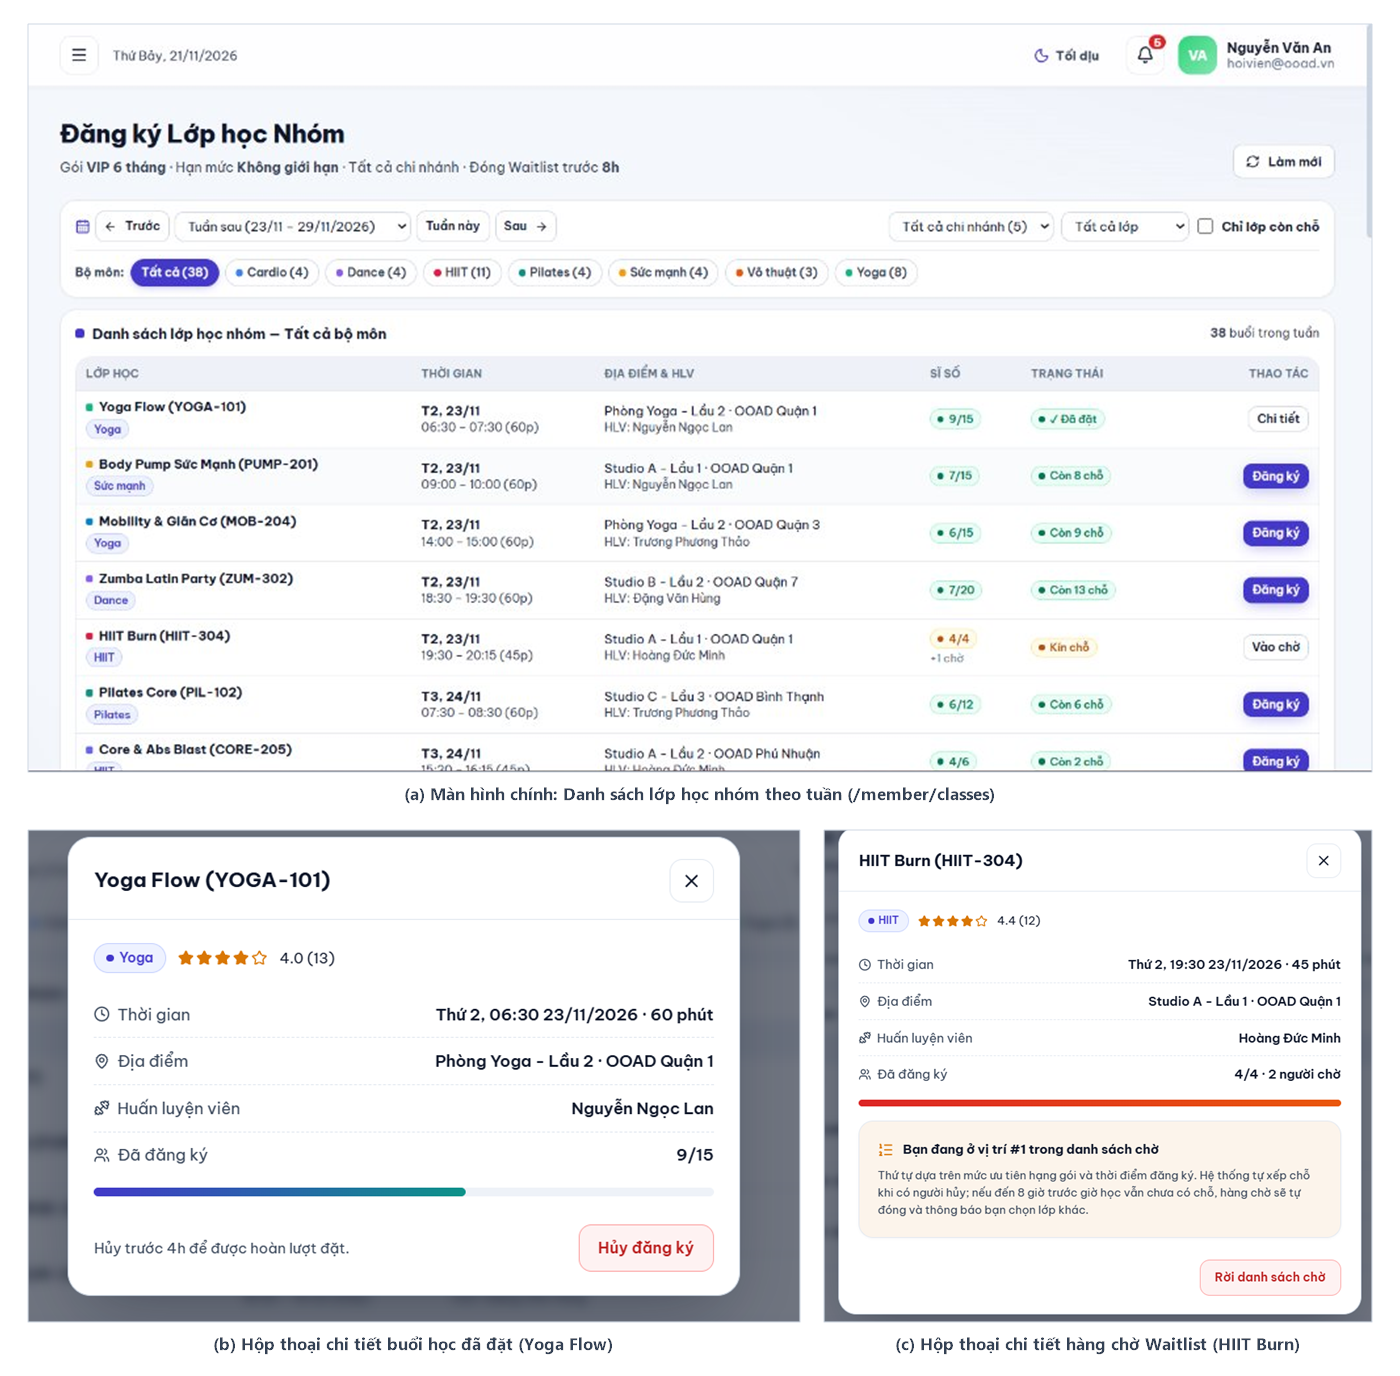
\includegraphics[width=0.96\textwidth]{images/ui_member_classes.png}
\caption{Giao diện màn hình Đăng ký Lớp học Nhóm và hộp thoại chi tiết đặt chỗ / hàng chờ Waitlist}
\label{fig:ui_member_classes}
\end{figure}

\par\medskip\noindent\textbf{Danh sách các thành phần giao diện}\par\smallskip
{\footnotesize
\setlength{\tabcolsep}{2.5pt}
\begin{longtable}{|c|L{2.95cm}|L{1.85cm}|L{2.95cm}|L{2.75cm}|L{1.90cm}|L{2.05cm}|}
\hline
\textbf{STT} & \textbf{Tên} & \textbf{Kiểu} & \textbf{Ý nghĩa} & \textbf{Miền giá trị} & \textbf{Giá trị mặc định} & \textbf{Ghi chú} \\
\hline
\endfirsthead
\hline
\textbf{STT} & \textbf{Tên} & \textbf{Kiểu} & \textbf{Ý nghĩa} & \textbf{Miền giá trị} & \textbf{Giá trị mặc định} & \textbf{Ghi chú} \\
\hline
\endhead
\hline
\endfoot
\hline
\caption{Danh sách các thành phần giao diện -- Màn hình Đăng ký Lớp học Nhóm} \\
\endlastfoot

\multicolumn{7}{|l|}{\textbf{Phần 1: Màn hình chính -- Danh sách lớp học nhóm theo tuần (Hình a)}} \\ \hline
1 & \texttt{Lbl\_TieuDe} & Label & Tiêu đề màn hình chức năng & Chuỗi ký tự & \texttt{"Đăng ký Lớp học Nhóm"} & Chỉ đọc \\ \hline
2 & \texttt{Lbl\_GoiHoiVien} & Label & Tóm tắt gói hội viên hiện hành, hạn mức đặt lớp, phạm vi chi nhánh và mốc đóng Waitlist & Chuỗi ký tự tổng hợp từ \texttt{Memberships} và tham số hệ thống & Thông tin gói đang hiệu lực của hội viên & Nhắc nhở nếu hội viên chưa có gói hợp lệ \\ \hline
3 & \texttt{Btn\_LamMoi} & Button & Tải lại danh sách buổi học và số liệu sĩ số mới nhất từ máy chủ & Trạng thái bình thường / đang tải & \texttt{"Làm mới"} & Vô hiệu hóa khi đang đồng bộ dữ liệu \\ \hline
4 & \texttt{Btn\_TuanTruoc} & Button & Chuyển lịch xem lùi 1 tuần so với tuần hiện tại & Kích hoạt / Vô hiệu & \texttt{"$\leftarrow$ Trước"} & Lùi \texttt{weekIdx} đi $1$ \\ \hline
5 & \texttt{Cbo\_ChonTuan} & ComboBox & Chọn nhanh tuần cần xem lịch học nhóm & Từ \texttt{Tuần trước} đến \texttt{Tuần +4} theo ngày Thứ Hai -- Chủ Nhật & \texttt{Tuần này} (tuần hiện tại) & Định dạng nhãn \texttt{dd/MM -- dd/MM/yyyy} \\ \hline
6 & \texttt{Btn\_TuanNay} & Button & Đưa lịch trở về tuần hiện tại (\texttt{weekIdx = 0}) & Kích hoạt / Vô hiệu & \texttt{"Tuần này"} (vô hiệu khi đang ở tuần hiện tại) & Hỗ trợ quay nhanh về tuần gốc \\ \hline
7 & \texttt{Btn\_TuanSau} & Button & Chuyển lịch xem tiến 1 tuần so với tuần đang chọn & Kích hoạt / Vô hiệu & \texttt{"Sau $\rightarrow$"} & Tăng \texttt{weekIdx} lên $1$ \\ \hline
8 & \texttt{Cbo\_ChiNhanh} & ComboBox & Lọc danh sách buổi học theo chi nhánh tổ chức & \texttt{"Tất cả chi nhánh (N)"} và các bản ghi từ bảng \texttt{Branches} & \texttt{"Tất cả chi nhánh"} & \texttt{N} là tổng số chi nhánh khả dụng \\ \hline
9 & \texttt{Cbo\_PhamVi} & ComboBox & Lọc theo toàn bộ lớp mở hoặc các lớp hội viên đã đặt / vào hàng chờ & \{\texttt{"Tất cả lớp"}, \texttt{"Lớp tôi đã đặt"}\} & \texttt{"Tất cả lớp"} & Kết hợp cùng bộ lọc chi nhánh \\ \hline
10 & \texttt{Chk\_ConCho} & Checkbox & Tùy chọn chỉ hiển thị những buổi học chưa đầy sĩ số và chưa bị hủy & \{\texttt{True}, \texttt{False}\} & \texttt{False} (chưa chọn) & Ẩn các buổi kín chỗ và buổi đã hủy \\ \hline
11 & \texttt{Chip\_BoMon} & Chip Button & Nhóm nút lọc nhanh theo bộ môn kèm số lượng buổi học tương ứng & \texttt{Tất cả (N)} và các bộ môn phát sinh trong tuần (\texttt{Cardio}, \texttt{Dance}, \texttt{HIIT}, \texttt{Pilates}, \texttt{Sức mạnh}, \texttt{Võ thuật}, \texttt{Yoga}, ...) & \texttt{"Tất cả"} & Tự cập nhật số lượng theo bộ lọc phía trên \\ \hline
12 & \texttt{Lbl\_TongBuoi} & Label & Tiêu đề khối bảng và tổng số buổi thỏa mãn điều kiện lọc & Số nguyên $\ge 0$ + nhãn mô tả & Tổng số buổi của tuần hiện tại & Cập nhật tức thời khi đổi bộ lọc \\ \hline
13 & \texttt{Grd\_BuoiHoc} & DataGrid & Bảng 6 cột (\textit{Lớp học}, \textit{Thời gian}, \textit{Địa điểm \& HLV}, \textit{Sĩ số}, \textit{Trạng thái}, \textit{Thao tác}) hiển thị các buổi học & Danh sách bản ghi từ \texttt{Class\_Sessions} sắp tăng dần theo \texttt{Start\_At} & Danh sách buổi học trong tuần thỏa bộ lọc & Cột \textit{Trạng thái} dùng nhãn màu phân biệt trực quan \\ \hline
14 & \texttt{Btn\_ThaoTac} & Button & Nút thao tác nhanh trên từng dòng để mở hộp thoại xử lý nghiệp vụ & \{\texttt{"Đăng ký"}, \texttt{"Vào chờ"}, \texttt{"Chi tiết"}, \texttt{"Xem chờ / Rời"}, \texttt{"Đã kín"}\} & Thay đổi động theo trạng thái buổi học và vé của hội viên & Mở \texttt{Dlg\_ChiTiet} của dòng được chọn \\ \hline

\multicolumn{7}{|l|}{\textbf{Phần 2: Hộp thoại chi tiết buổi học -- Đặt chỗ \& Hàng chờ Waitlist (Hình b, c)}} \\ \hline
15 & \texttt{Dlg\_ChiTiet} & Modal Dialog & Cửa sổ nổi hiển thị thông tin đầy đủ của một buổi học cụ thể & Trạng thái Đóng / Mở & Đóng & Hiển thị khi hội viên chọn dòng trên bảng \\ \hline
16 & \texttt{Lbl\_TenLop} & Label & Tên lớp và mã định danh lớp tập trên phần đầu hộp thoại & Chuỗi ký tự (\texttt{GymClass.Name}) & Tên lớp được chọn & Ví dụ: \texttt{Yoga Flow (YOGA-101)} \\ \hline
17 & \texttt{Btn\_Dong} & Button & Nút \texttt{$\times$} đóng hộp thoại chi tiết và quay về danh sách & Kích hoạt & \texttt{"$\times$"} & Có thể đóng bằng cách nhấp vùng nền mờ \\ \hline
18 & \texttt{Lbl\_DanhGia} & Badge / Label & Nhãn bộ môn, nhãn trạng thái đặc biệt và điểm sao trung bình kèm số lượt đánh giá & \texttt{Category}, trạng thái (\texttt{Đã hủy} / \texttt{Đã hoàn thành}), điểm $1.0$--$5.0$ & Điểm sao trung bình tổng hợp từ \texttt{Reviews} & Ví dụ: \texttt{4.0 (13)} ở Hình (b) \\ \hline
19 & \texttt{Lbl\_ThongTin} & Label Group & 4 dòng thông tin chi tiết: \textit{Thời gian}, \textit{Địa điểm}, \textit{Huấn luyện viên}, \textit{Đã đăng ký} & Ngày giờ, thời lượng, phòng, chi nhánh, tên HLV, \texttt{booked/capacity} và số người chờ & Lấy từ bản ghi buổi học & Ví dụ: \texttt{4/4 \textperiodcentered\ 2 người chờ} ở Hình (c) \\ \hline
20 & \texttt{Prg\_SiSo} & ProgressBar & Thanh tiến độ tỷ lệ lấp đầy chỗ của buổi học & $0\% \rightarrow 100\%$ (\texttt{booked / capacity}) & Theo tỷ lệ sĩ số hiện tại & Đổi sang sắc đỏ--cam khi lớp đủ $100\%$ sĩ số \\ \hline
21 & \texttt{Pnl\_HangCho} & Alert Panel & Hộp thông báo vị trí chờ \texttt{\#k}, quy tắc ưu tiên hạng gói và mốc đóng Waitlist $8\text{h}$, hoặc cảnh báo đóng hàng chờ & Hiển thị / Ẩn theo ngữ cảnh \texttt{Waitlist\_Entries} & Ẩn (chỉ hiện khi đang chờ hoặc kín lớp $\le 8\text{h}$) & Hiện nền vàng cam khi đang chờ (Hình c); nền đỏ khi quá mốc $8\text{h}$ \\ \hline
22 & \texttt{Lbl\_ChinhSach} & Label & Ghi chú chính sách hủy lịch trước $4\text{h}$ để được hoàn lượt hoặc cảnh báo hủy trễ & Chuỗi quy tắc hủy động theo thời điểm hiện tại & Hiện khi hội viên đang ở trạng thái \texttt{Đã đặt} & Ví dụ: \texttt{"Hủy trước 4h để được hoàn lượt đặt."} (Hình b) \\ \hline
23 & \texttt{Btn\_HanhDong} & Button & Nút thực hiện giao dịch đặt chỗ, vào hàng chờ hoặc hủy lịch theo ngữ cảnh & \{\texttt{"Đặt chỗ ngay"}, \texttt{"Vào danh sách chờ"}, \texttt{"Hủy đăng ký"}, \texttt{"Rời danh sách chờ"}, \texttt{"Đã diễn ra"}, \texttt{"Buổi đã hủy"}\} & Tự đổi nhãn và màu sắc theo điều kiện nghiệp vụ & Vô hiệu hóa khi lớp đã qua, đã hủy hoặc lớp đầy và còn $\le 8\text{h}$ \\ \hline

\end{longtable}
}

\par\medskip\noindent\textbf{Danh sách các biến cố}\par\smallskip
{\footnotesize
\setlength{\tabcolsep}{4pt}
\begin{longtable}{|c|L{3.5cm}|L{7.8cm}|L{3.5cm}|}
\hline
\textbf{STT} & \textbf{Điều kiện kích hoạt} & \textbf{Xử lý} & \textbf{Ghi chú} \\
\hline
\endfirsthead
\hline
\textbf{STT} & \textbf{Điều kiện kích hoạt} & \textbf{Xử lý} & \textbf{Ghi chú} \\
\hline
\endhead
\hline
\endfoot
\hline
\caption{Danh sách các biến cố -- Màn hình Đăng ký Lớp học Nhóm} \\
\endlastfoot

0 & Khởi động màn hình (\texttt{/member/classes}) &
Hệ thống xác định khoảng ngày Thứ Hai -- Chủ Nhật của tuần mặc định (\texttt{Tuần này}); tải thông tin gói hội viên hiệu lực của người dùng lên \texttt{Lbl\_GoiHoiVien}; nạp danh sách chi nhánh vào \texttt{Cbo\_ChiNhanh}; truy vấn \texttt{Class\_Sessions} trong tuần cùng trạng thái đặt chỗ / hàng chờ cá nhân; thống kê số buổi theo bộ môn lên \texttt{Chip\_BoMon} và hiển thị danh sách lên \texttt{Grd\_BuoiHoc} kèm \texttt{Lbl\_TongBuoi}. &
Đóng \texttt{Dlg\_ChiTiet}; vô hiệu hóa nút \texttt{Btn\_TuanNay} khi đang ở tuần hiện tại. \\ \hline

1 & Nhấn nút \texttt{Btn\_LamMoi} (\textit{Làm mới}) &
Chuyển trạng thái nút sang \texttt{"Đang tải..."}, gọi API tải lại danh sách buổi học trong tuần đang chọn, danh mục chi nhánh và hạn mức gói mới nhất; cập nhật lại đồng hồ thời gian hiện tại và kết xuất lại \texttt{Grd\_BuoiHoc}. &
Đảm bảo sĩ số và vị trí chờ luôn đồng bộ trước khi thao tác. \\ \hline

2 & Điều hướng tuần bằng \texttt{Btn\_TuanTruoc}, \texttt{Btn\_TuanSau}, \texttt{Btn\_TuanNay} hoặc đổi giá trị \texttt{Cbo\_ChonTuan} &
Cập nhật chỉ số tuần \texttt{weekIdx} (giảm $1$, tăng $1$, về $0$ hoặc theo mục đã chọn), tính lại 7 ngày trong tuần mới, truy vấn lại danh sách \texttt{Class\_Sessions} thuộc tuần đó, cập nhật lại trạng thái nút \texttt{Btn\_TuanNay}, bộ đếm trên \texttt{Chip\_BoMon} và làm mới bảng \texttt{Grd\_BuoiHoc}. &
Cho phép xem và đặt trước các tuần kế tiếp trong phạm vi hỗ trợ. \\ \hline

3 & Thay đổi lựa chọn trên \texttt{Cbo\_ChiNhanh}, \texttt{Cbo\_PhamVi} hoặc bật/tắt \texttt{Chk\_ConCho} &
Thực hiện lọc tức thời danh sách buổi học của tuần hiện tại theo: (i) chi nhánh được chọn, (ii) phạm vi toàn bộ lớp hay chỉ \textit{Lớp tôi đã đặt}, (iii) ẩn các lớp kín chỗ hoặc đã hủy nếu bật \texttt{Chk\_ConCho}; sắp xếp tăng dần theo \texttt{Start\_At}, tính lại bộ đếm từng bộ môn trên \texttt{Chip\_BoMon} và cập nhật \texttt{Grd\_BuoiHoc}, \texttt{Lbl\_TongBuoi}. &
Nếu bộ môn đang chọn không còn buổi nào khớp bộ lọc, tự đưa \texttt{Chip\_BoMon} về \texttt{"Tất cả"}. \\ \hline

4 & Chọn một bộ môn trong nhóm \texttt{Chip\_BoMon} &
Đánh dấu nổi bật chip bộ môn được chọn; lọc các buổi học hiển thị trong \texttt{Grd\_BuoiHoc} theo đúng \texttt{Category} tương ứng (hoặc bỏ lọc bộ môn nếu chọn \texttt{"Tất cả"}); đổi tiêu đề bảng và số lượng trên \texttt{Lbl\_TongBuoi}. &
Không cần gọi lại máy chủ do lọc trên dữ liệu tuần đã nạp. \\ \hline

5 & Nhấn vào một dòng trên \texttt{Grd\_BuoiHoc} hoặc nút \texttt{Btn\_ThaoTac} tương ứng &
Mở hộp thoại \texttt{Dlg\_ChiTiet}; tải thông tin chi tiết mới nhất của buổi học gồm điểm đánh giá từ \texttt{Reviews}, thanh tiến độ \texttt{Prg\_SiSo}, vị trí chờ (nếu có); xác định ngữ cảnh hiển thị cho \texttt{Pnl\_HangCho}, \texttt{Lbl\_ChinhSach} và nhãn/trạng thái khả dụng của \texttt{Btn\_HanhDong}. &
Hiển thị dạng Hình~(b) nếu đã đặt chỗ, hoặc Hình~(c) nếu đang trong Waitlist. \\ \hline

6 & Nhấn nút \texttt{Btn\_HanhDong} ở trạng thái \textit{"Đặt chỗ ngay"} (còn chỗ) &
Kiểm tra các điều kiện nghiệp vụ: gói hội viên còn hiệu lực và áp dụng tại chi nhánh của lớp, chưa vượt hạn mức lượt đặt lớp/tháng (\texttt{Max\_Bookings\_Per\_Month}), hội viên chưa đặt buổi này và không trùng khung giờ với buổi/lịch PT khác, buổi học chưa diễn ra và còn chỗ trống. Nếu hợp lệ, ghi nhận bản ghi vào \texttt{Bookings} (trạng thái \texttt{Confirmed}), trừ hạn mức (nếu gói có giới hạn), thông báo thành công và cập nhật lại hộp thoại cùng \texttt{Grd\_BuoiHoc}. &
Nếu vi phạm ràng buộc nghiệp vụ, hiển thị thông báo lỗi cụ thể và giữ nguyên trạng thái. \\ \hline

7 & Nhấn nút \texttt{Btn\_HanhDong} ở trạng thái \textit{"Vào danh sách chờ"} (lớp đã kín và còn $> 8\text{h}$) &
Kiểm tra điều kiện hợp lệ (gói hiệu lực, phạm vi chi nhánh, không trùng lịch, còn trên $8\text{h}$ trước giờ bắt đầu). Ghi nhận bản ghi vào \texttt{Waitlist\_Entries} kèm điểm ưu tiên theo hạng gói và thời điểm đăng ký; tính thứ tự chờ \texttt{\#k}; thông báo kết quả và chuyển \texttt{Dlg\_ChiTiet} sang giao diện hiển thị \texttt{Pnl\_HangCho} (Hình c). &
Nếu từ $\le 8\text{h}$ trước giờ học, hệ thống đóng chức năng vào chờ và vô hiệu hóa thao tác. \\ \hline

8 & Nhấn nút \texttt{Btn\_HanhDong} ở trạng thái \textit{"Hủy đăng ký"} (Hình b) &
Kiểm tra buổi học chưa bắt đầu; tính khoảng thời gian còn lại so với mốc hủy hợp lệ ($4\text{h}$): nếu $\ge 4\text{h}$ thì cập nhật hủy vé và hoàn lại lượt đặt vào hạn mức gói, nếu $< 4\text{h}$ vẫn ghi nhận hủy nhưng không hoàn lượt. Đồng thời kích hoạt cơ chế tự động đôn người đứng đầu đủ điều kiện từ \texttt{Waitlist\_Entries} lên \texttt{Confirmed} (nếu còn chỗ trống), thông báo kết quả, đóng \texttt{Dlg\_ChiTiet} và làm mới \texttt{Grd\_BuoiHoc}. &
Chỗ trống được nhường tự động cho hội viên ưu tiên cao nhất trong hàng chờ. \\ \hline

9 & Nhấn nút \texttt{Btn\_HanhDong} ở trạng thái \textit{"Rời danh sách chờ"} (Hình c) &
Xóa hoặc chuyển trạng thái rời hàng chờ cho bản ghi \texttt{Waitlist\_Entries} của hội viên ở buổi học hiện tại; sắp xếp lại thứ tự \texttt{\#k} cho các hội viên chờ phía sau; hiển thị thông báo đã rời hàng chờ, đóng \texttt{Dlg\_ChiTiet} và cập nhật lại bảng \texttt{Grd\_BuoiHoc}. &
Không trừ lượt đặt trong hạn mức gói của hội viên. \\ \hline

10 & Nhấn nút \texttt{Btn\_Dong} ($\times$) hoặc nhấp ra ngoài khung hộp thoại \texttt{Dlg\_ChiTiet} &
Đặt trạng thái phiên được chọn về rỗng (\texttt{null}), đóng hộp thoại \texttt{Dlg\_ChiTiet} và trả lại quyền tương tác cho danh sách \texttt{Grd\_BuoiHoc}. &
Không làm thay đổi dữ liệu hoặc bộ lọc đang áp dụng. \\ \hline

\end{longtable}
}


\subsubsection{Màn hình Thời khóa biểu cá nhân của tôi (Hội viên)}
Màn hình \textbf{Thời Khóa Biểu Cá Nhân Của Tôi} (đường dẫn \texttt{/member/bookings}) cho phép \textbf{Hội viên} theo dõi toàn bộ lịch \textbf{Lớp học nhóm} và \textbf{PT 1-kèm-1} đã đăng ký theo hai chế độ hiển thị linh hoạt: thời khóa biểu dạng bảng tuần ($10$ ca chuẩn $\times$ $7$ ngày) và danh sách theo dòng thời gian, đồng thời hỗ trợ hủy lịch đúng hạn hoặc đánh giá buổi học sau khi đã tham gia.

Giao diện được tổ chức theo 3 khung chính minh họa ở Hình~\ref{fig:ui_member_bookings}:
\begin{itemize}
    \item \textbf{Hình (a) -- Thời khóa biểu dạng tuần:} Bố trí theo $7$ cột Thứ Hai -- Chủ Nhật và $10$ hàng ca tập (\texttt{Ca 1} đến \texttt{Ca 10}), phân biệt trực quan bằng màu sắc giữa lớp nhóm, buổi PT và trạng thái chờ Waitlist.
    \item \textbf{Hình (b) -- Danh sách lịch Sắp tới:} Liệt kê các buổi học chuẩn bị diễn ra theo thứ tự thời gian, hỗ trợ lọc theo loại hình và nút \texttt{Hủy} / \texttt{Rời chờ} nhanh.
    \item \textbf{Hình (c) -- Lịch sử \& Đánh giá:} Tổng hợp các buổi đã hoàn thành hoặc đã hủy trước đó, mở nút \texttt{Đánh giá} cho các buổi đã check-in tham gia hợp lệ.
\end{itemize}

\begin{figure}[H]
\centering
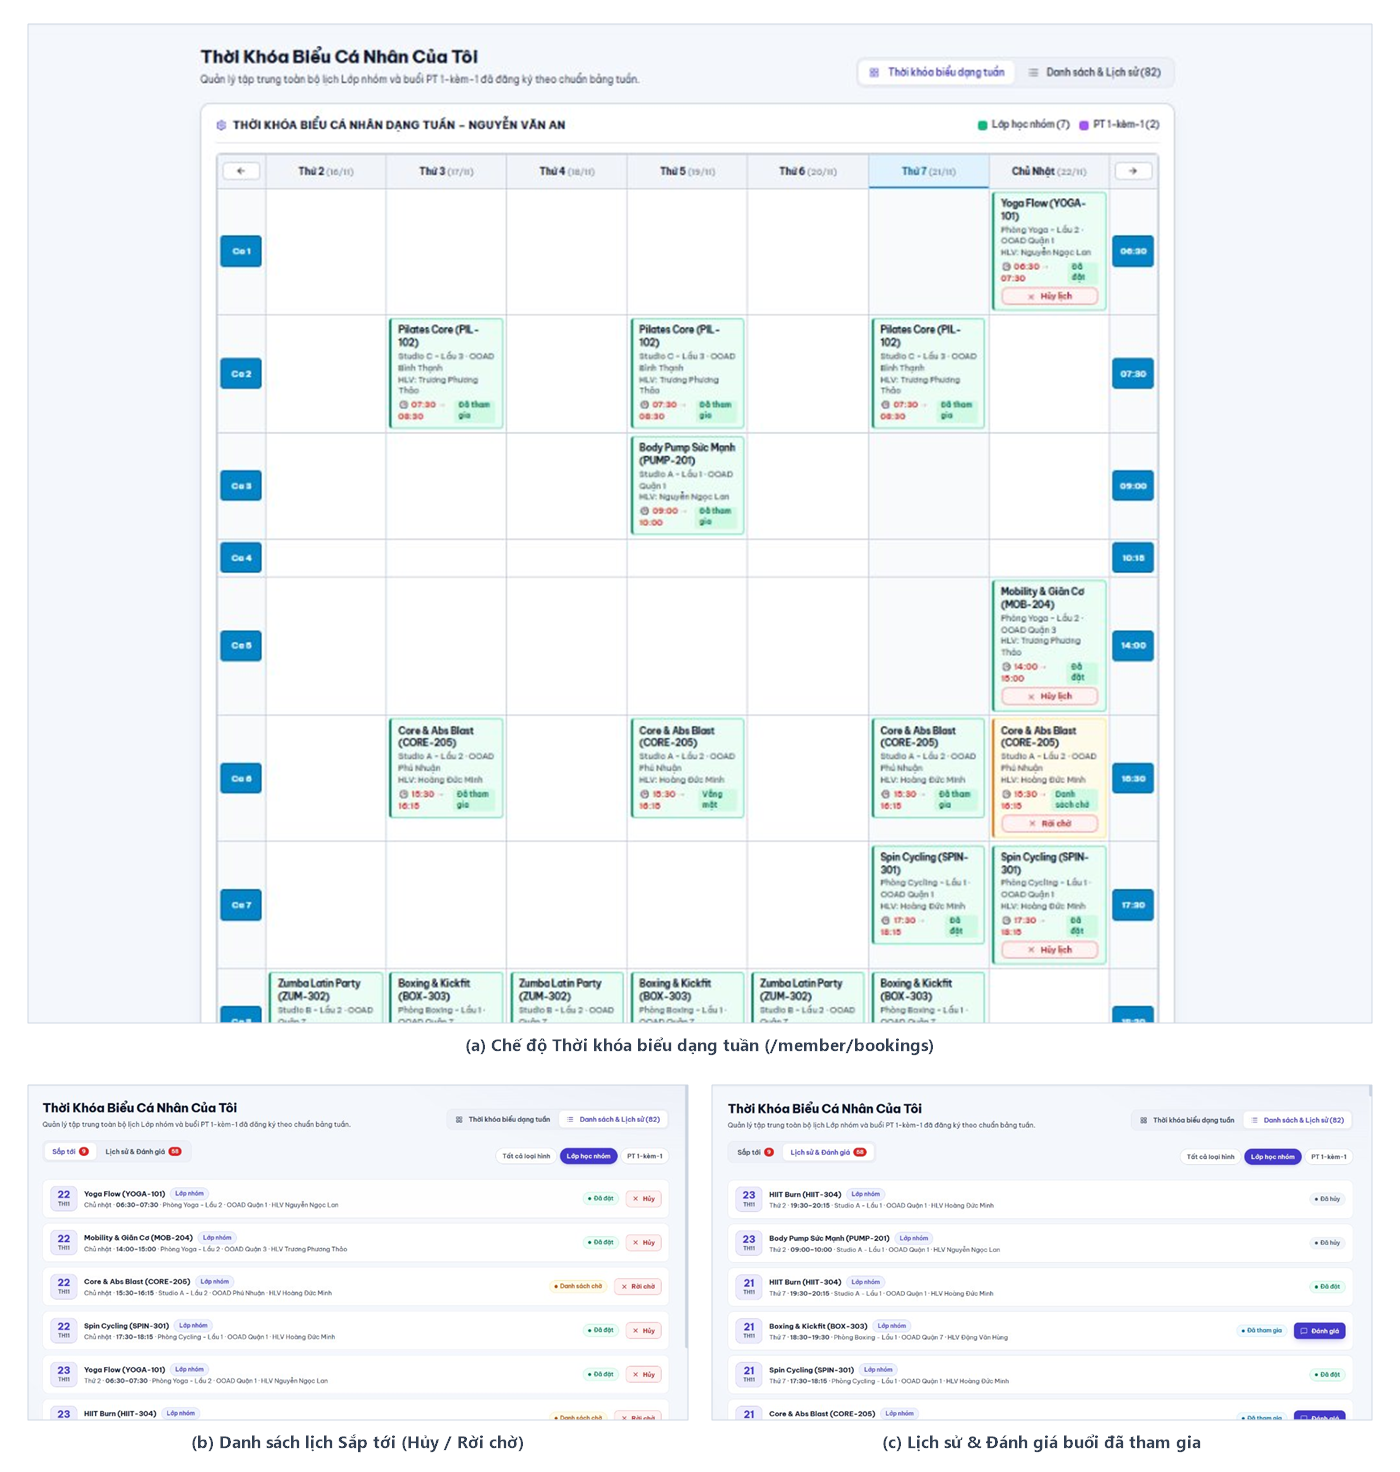
\includegraphics[width=0.96\textwidth]{images/ui_member_bookings.png}
\caption{Giao diện màn hình Thời khóa biểu cá nhân của tôi (dạng tuần, lịch Sắp tới và Lịch sử \& Đánh giá)}
\label{fig:ui_member_bookings}
\end{figure}

\par\medskip\noindent\textbf{Danh sách các thành phần giao diện}\par\smallskip
{\footnotesize
\setlength{\tabcolsep}{2.5pt}
\begin{longtable}{|c|L{2.95cm}|L{1.85cm}|L{2.95cm}|L{2.75cm}|L{1.90cm}|L{2.05cm}|}
\hline
\textbf{STT} & \textbf{Tên} & \textbf{Kiểu} & \textbf{Ý nghĩa} & \textbf{Miền giá trị} & \textbf{Giá trị mặc định} & \textbf{Ghi chú} \\
\hline
\endfirsthead
\hline
\textbf{STT} & \textbf{Tên} & \textbf{Kiểu} & \textbf{Ý nghĩa} & \textbf{Miền giá trị} & \textbf{Giá trị mặc định} & \textbf{Ghi chú} \\
\hline
\endhead
\hline
\endfoot
\hline
\caption{Danh sách các thành phần giao diện -- Màn hình Thời khóa biểu cá nhân của tôi} \\
\endlastfoot

\multicolumn{7}{|l|}{\textbf{Phần 1: Thanh tiêu đề \& Chuyển đổi chế độ hiển thị}} \\ \hline
1 & \texttt{Lbl\_TieuDeLich} & Label & Tiêu đề màn hình và thông tin tóm tắt lượt đặt trong tháng của gói hội viên & Chuỗi ký tự & \texttt{"Thời Khóa Biểu Cá Nhân Của Tôi"} & Kèm dòng mô tả gói đang hiệu lực (chế độ API) \\ \hline
2 & \texttt{Btn\_LamMoiLich} & Button & Tải lại dữ liệu đặt lớp, hàng chờ và lịch PT mới nhất từ máy chủ & Kích hoạt / Đang tải & \texttt{"Làm mới"} & Chỉ hiển thị khi đang kết nối máy chủ API \\ \hline
3 & \texttt{Tab\_CheDoXem} & Tab Group & Chuyển đổi giữa xem bảng thời khóa biểu tuần và xem danh sách lịch sử & \{\texttt{"Thời khóa biểu dạng tuần"}, \texttt{"Danh sách \& Lịch sử (N)"}\} & \texttt{"Thời khóa biểu dạng tuần"} & \texttt{N} là tổng số bản ghi lịch cá nhân \\ \hline

\multicolumn{7}{|l|}{\textbf{Phần 2: Chế độ Thời khóa biểu dạng tuần (Hình a)}} \\ \hline
4 & \texttt{Lbl\_TieuDeTKB} & Label Group & Tiêu đề bảng tuần theo tên hội viên và chú giải màu theo loại hình buổi tập & Chuỗi tên + số lượng \textit{Lớp học nhóm}, \textit{PT 1-kèm-1} & Hiển thị theo danh sách lịch sắp tới & Xanh lá: Lớp nhóm; Tím: PT 1-kèm-1 \\ \hline
5 & \texttt{Btn\_DieuHuongTuan} & Button Pair & Hai nút \texttt{$\leftarrow$} và \texttt{$\rightarrow$} ở hai góc tiêu đề bảng để chuyển tuần lùi hoặc tiến & Chỉ số tuần \texttt{weekIdx} $\in \{-1, 0, 1\}$ & \texttt{weekIdx = 0} (tuần hiện tại) & Vô hiệu hóa ở biên $-1$ và $+1$ \\ \hline
6 & \texttt{Tbl\_ThoiKhoaBieu} & Matrix Table & Lưới thời khóa biểu $10$ ca (\texttt{Ca 1}--\texttt{Ca 10}, khung giờ $06:30$--$20:30$) $\times$ $7$ ngày (Thứ Hai -- Chủ Nhật) & Các bản ghi đặt chỗ hiệu lực và buổi đã tham gia trong tuần & Tuần hiện tại & Đánh dấu nổi bật cột ngày hiện tại \\ \hline
7 & \texttt{Card\_BuoiTKB} & Card Item & Thẻ buổi tập đặt trong từng ô ca--ngày gồm tên lớp/PT, phòng, HLV, giờ và nhãn trạng thái & \texttt{Đã đặt}, \texttt{Đã tham gia}, \texttt{Vắng mặt}, \texttt{Danh sách chờ}, \texttt{Đã xác nhận} & Theo trạng thái từng bản ghi & Khung cam với thẻ đang ở hàng chờ \\ \hline
8 & \texttt{Btn\_\hspace{0pt}HuyTrenTKB} & Button & Nút \texttt{Hủy lịch} hoặc \texttt{Rời chờ} gắn trực tiếp trên thẻ buổi sắp tới & Kích hoạt khi buổi chưa kết thúc & Ẩn với các buổi đã diễn ra & Mở hộp thoại xác nhận \texttt{Dlg\_\hspace{0pt}XacNhanHuy} \\ \hline

\multicolumn{7}{|l|}{\textbf{Phần 3: Chế độ Danh sách \& Lịch sử và Các hộp thoại (Hình b, c)}} \\ \hline
9 & \texttt{Tab\_SapToiLichSu} & Tab Group & Phân tách danh sách \texttt{Sắp tới} và \texttt{Lịch sử \& Đánh giá} & \{\texttt{"Sắp tới"}, \texttt{"Lịch sử \& Đánh giá"}\} & \texttt{"Sắp tới"} & Hiện số lịch sắp tới và số buổi chờ đánh giá \\ \hline
10 & \texttt{Chip\_LoaiHinh} & Chip Button & Nhóm chip lọc danh sách theo loại hình tập luyện & \{\texttt{"Tất cả loại hình"}, \texttt{"Lớp học nhóm"}, \texttt{"PT 1-kèm-1"}\} & \texttt{"Tất cả loại hình"} & Áp dụng chung cho cả 2 tab danh sách \\ \hline
11 & \texttt{Lst\_LichCaNhan} & List View & Danh sách thẻ chi tiết gồm hộp ngày/tháng, tên buổi, khung giờ, chi nhánh, HLV và badge trạng thái & Dữ liệu tổng hợp từ \texttt{Bookings} và \texttt{Waitlist\_Entries} & Sắp tăng dần (Sắp tới) / giảm dần (Lịch sử) & Hiển thị trạng thái \textit{Empty} khi rỗng \\ \hline
12 & \texttt{Btn\_\hspace{0pt}HuyHoacRoi} & Button & Nút \texttt{Hủy} (vé đã đặt) hoặc \texttt{Rời chờ} (hàng chờ) ở từng dòng tab \textit{Sắp tới} & Kích hoạt khi \texttt{Start\_At} $>$ hiện tại & Chỉ hiện ở các dòng còn quyền hủy & Mở \texttt{Dlg\_\hspace{0pt}XacNhanHuy} \\ \hline
13 & \texttt{Btn\_DanhGia} & Button / Badge & Nút \texttt{Đánh giá} cho phép chấm sao buổi đã tham gia hoặc nhãn \texttt{Đã đánh giá} nếu đã gửi & Trạng thái chưa đánh giá / đã đánh giá & Chỉ hiện ở tab \textit{Lịch sử} với buổi đạt \texttt{Attended} & Mở hộp thoại \texttt{Dlg\_DanhGia} \\ \hline
14 & \texttt{Dlg\_XacNhanHuy} & Confirm Dialog & Hộp thoại cảnh báo chính sách hoàn lượt (trước $4\text{h}$) hoặc mất lượt ($< 4\text{h}$) kèm nút \texttt{Xác nhận hủy} & Đóng / Mở & Đóng & Thực thi hủy vé hoặc rời Waitlist \\ \hline
15 & \texttt{Dlg\_DanhGia} & Modal Dialog & Hộp thoại chọn đánh giá $1$--$5$ sao, ô nhập nhận xét và nút \texttt{Gửi đánh giá} & Đóng / Mở; điểm $1$--$5$ & Đóng ($5$ sao mặc định khi mở) & Lưu bản ghi vào bảng \texttt{Reviews} \\ \hline

\end{longtable}
}

\par\medskip\noindent\textbf{Danh sách các biến cố}\par\smallskip
{\footnotesize
\setlength{\tabcolsep}{4pt}
\begin{longtable}{|c|L{3.5cm}|L{7.8cm}|L{3.5cm}|}
\hline
\textbf{STT} & \textbf{Điều kiện kích hoạt} & \textbf{Xử lý} & \textbf{Ghi chú} \\
\hline
\endfirsthead
\hline
\textbf{STT} & \textbf{Điều kiện kích hoạt} & \textbf{Xử lý} & \textbf{Ghi chú} \\
\hline
\endhead
\hline
\endfoot
\hline
\caption{Danh sách các biến cố -- Màn hình Thời khóa biểu cá nhân của tôi} \\
\endlastfoot

0 & Khởi động màn hình (\texttt{/member/bookings}) &
Hệ thống nạp toàn bộ lịch đặt lớp nhóm, lịch PT 1-kèm-1 và mục hàng chờ Waitlist của hội viên; phân nhóm thành lịch \textit{Sắp tới} và \textit{Lịch sử}; mặc định mở chế độ \texttt{Thời khóa biểu dạng tuần} với \texttt{weekIdx = 0} và đặt các thẻ buổi tập vào đúng ô \texttt{Ca 1}--\texttt{Ca 10} $\times$ $7$ ngày. &
Nếu người dùng mới hủy/đặt lịch trước đó, dữ liệu phản ánh ngay trạng thái mới nhất. \\ \hline

1 & Chọn tab trên \texttt{Tab\_CheDoXem} (\textit{Thời khóa biểu dạng tuần} / \textit{Danh sách \& Lịch sử}) &
Chuyển giao diện nội dung giữa bảng ma trận tuần (\texttt{Tbl\_ThoiKhoaBieu}) và chế độ danh sách chi tiết (\texttt{Lst\_LichCaNhan}). Khi chuyển sang bảng tuần, tự đưa tab danh sách về \texttt{"Sắp tới"}. &
Giữ nguyên toàn bộ dữ liệu đã nạp mà không cần gọi lại API. \\ \hline

2 & Nhấn nút điều hướng \texttt{$\leftarrow$} hoặc \texttt{$\rightarrow$} trên \texttt{Btn\_DieuHuongTuan} &
Thay đổi \texttt{weekIdx} trong phạm vi $\{-1, 0, 1\}$, tính lại $7$ ngày Thứ Hai -- Chủ Nhật của tuần tương ứng và lọc các thẻ buổi tập rơi vào tuần mới lên \texttt{Tbl\_ThoiKhoaBieu}. &
Hỗ trợ đối chiếu lịch tuần trước, tuần này và tuần kế tiếp. \\ \hline

3 & Chuyển tab \texttt{Tab\_SapToiLichSu} (\textit{Sắp tới} / \textit{Lịch sử \& Đánh giá}) &
Chuyển danh sách nguồn của \texttt{Lst\_LichCaNhan} sang các buổi đang hiệu lực (sắp tăng dần theo giờ học) hoặc lịch sử tập luyện/đã hủy (sắp giảm dần theo giờ học). &
Tab \textit{Lịch sử} hiển thị thêm số buổi chưa đánh giá để nhắc hội viên. \\ \hline

4 & Chọn bộ lọc trong \texttt{Chip\_LoaiHinh} &
Đánh dấu chip được chọn và lọc các dòng trong \texttt{Lst\_LichCaNhan} theo toàn bộ, chỉ \textit{Lớp học nhóm} hoặc chỉ \textit{PT 1-kèm-1}. &
Không ảnh hưởng đến số lượng tổng trên tiêu đề tab. \\ \hline

5 & Nhấn nút \texttt{Btn\_HuyTrenTKB} hoặc \texttt{Btn\_HuyHoacRoi} (\textit{Hủy} / \textit{Rời chờ}) &
Mở hộp thoại \texttt{Dlg\_XacNhanHuy}, hiển thị tên buổi, thời gian học và thông báo rõ trường hợp hủy đúng hạn (trước $4\text{h}$ hoặc đang chờ $\rightarrow$ hoàn lượt) hay quá hạn ($< 4\text{h}$ $\rightarrow$ tính đã sử dụng). &
Tránh thao tác hủy nhầm gây mất lượt tập của hội viên. \\ \hline

6 & Nhấn \texttt{Xác nhận hủy} trong \texttt{Dlg\_XacNhanHuy} &
Nếu là mục hàng chờ Waitlist, xóa khỏi \texttt{Waitlist\_Entries} và không trừ lượt; nếu là vé lớp nhóm/PT, cập nhật trạng thái hủy, xử lý hoàn/không hoàn lượt theo mốc $4\text{h}$ và tự động đôn người ưu tiên cao nhất trong hàng chờ (nếu là lớp nhóm). Sau đó đóng hộp thoại và tải lại lịch. &
Gửi thông báo xác nhận kết quả hoàn lượt bằng Toast. \\ \hline

7 & Nhấn nút \texttt{Btn\_DanhGia} trên một buổi đã tham gia ở tab \textit{Lịch sử} &
Mở hộp thoại \texttt{Dlg\_DanhGia} gắn với buổi học hoặc buổi PT được chọn, khởi tạo sẵn $5$ sao và ô nhận xét rỗng. &
Chỉ mở với các buổi có trạng thái \texttt{Attended} / \texttt{Completed} và chưa từng đánh giá. \\ \hline

8 & Chọn số sao, nhập nhận xét và nhấn \texttt{Gửi đánh giá} trong \texttt{Dlg\_DanhGia} &
Ghi nhận bản ghi mới vào bảng \texttt{Reviews} (gồm điểm $1$--$5$, nhận xét, mã buổi đặt), hiển thị lời cảm ơn, đóng hộp thoại và cập nhật dòng tương ứng thành nhãn \texttt{Đã đánh giá}. &
Điểm đánh giá được tổng hợp vào điểm trung bình của lớp/HLV. \\ \hline

9 & Nhấn nút \texttt{Btn\_LamMoiLich} (\textit{Làm mới}) &
Gọi API lấy lại lịch sử đặt chỗ, trạng thái điểm danh và danh sách Waitlist mới nhất từ máy chủ, cập nhật lại đồng loạt cả TKB tuần và tab danh sách. &
Chỉ khả dụng khi ứng dụng đang kết nối với API máy chủ. \\ \hline

\end{longtable}
}


\subsubsection{Màn hình Lớp dạy và Điểm danh (Huấn luyện viên)}
Màn hình \textbf{Lớp dạy \& điểm danh} (đường dẫn \texttt{/trainer/classes}) hỗ trợ \textbf{Huấn luyện viên (HLV)} quản lý toàn bộ các buổi dạy được phân công theo trạng thái và thực hiện điểm danh học viên đầu/trong buổi học có đối chiếu tự động dữ liệu Check-in tại chi nhánh cùng danh sách chờ Waitlist.

Giao diện gồm các thành phần trực quan được tổng hợp trong Hình~\ref{fig:ui_trainer_classes}:
\begin{itemize}
    \item \textbf{Hình (a) -- Tab Cần điểm danh:} Hiển thị các buổi dạy đã đến/qua giờ bắt đầu nhưng chưa chốt điểm danh để HLV mở bảng ghi nhận chuyên cần kịp thời.
    \item \textbf{Hình (b) -- Tab Sắp tới:} Liệt kê lịch dạy sắp diễn ra với sĩ số hiện tại (\texttt{booked/capacity}) và cảnh báo số học viên đang nằm trong danh sách chờ.
    \item \textbf{Hình (c) -- Hộp thoại Điểm danh buổi học:} Bảng $4$ cột đối chiếu trực tiếp cột \textit{Check-in tại CN} (tự động tích chọn trước học viên đã quẹt thẻ hợp lệ tại chi nhánh) kèm khối \textit{Danh sách chờ} phía dưới.
\end{itemize}

\begin{figure}[H]
\centering
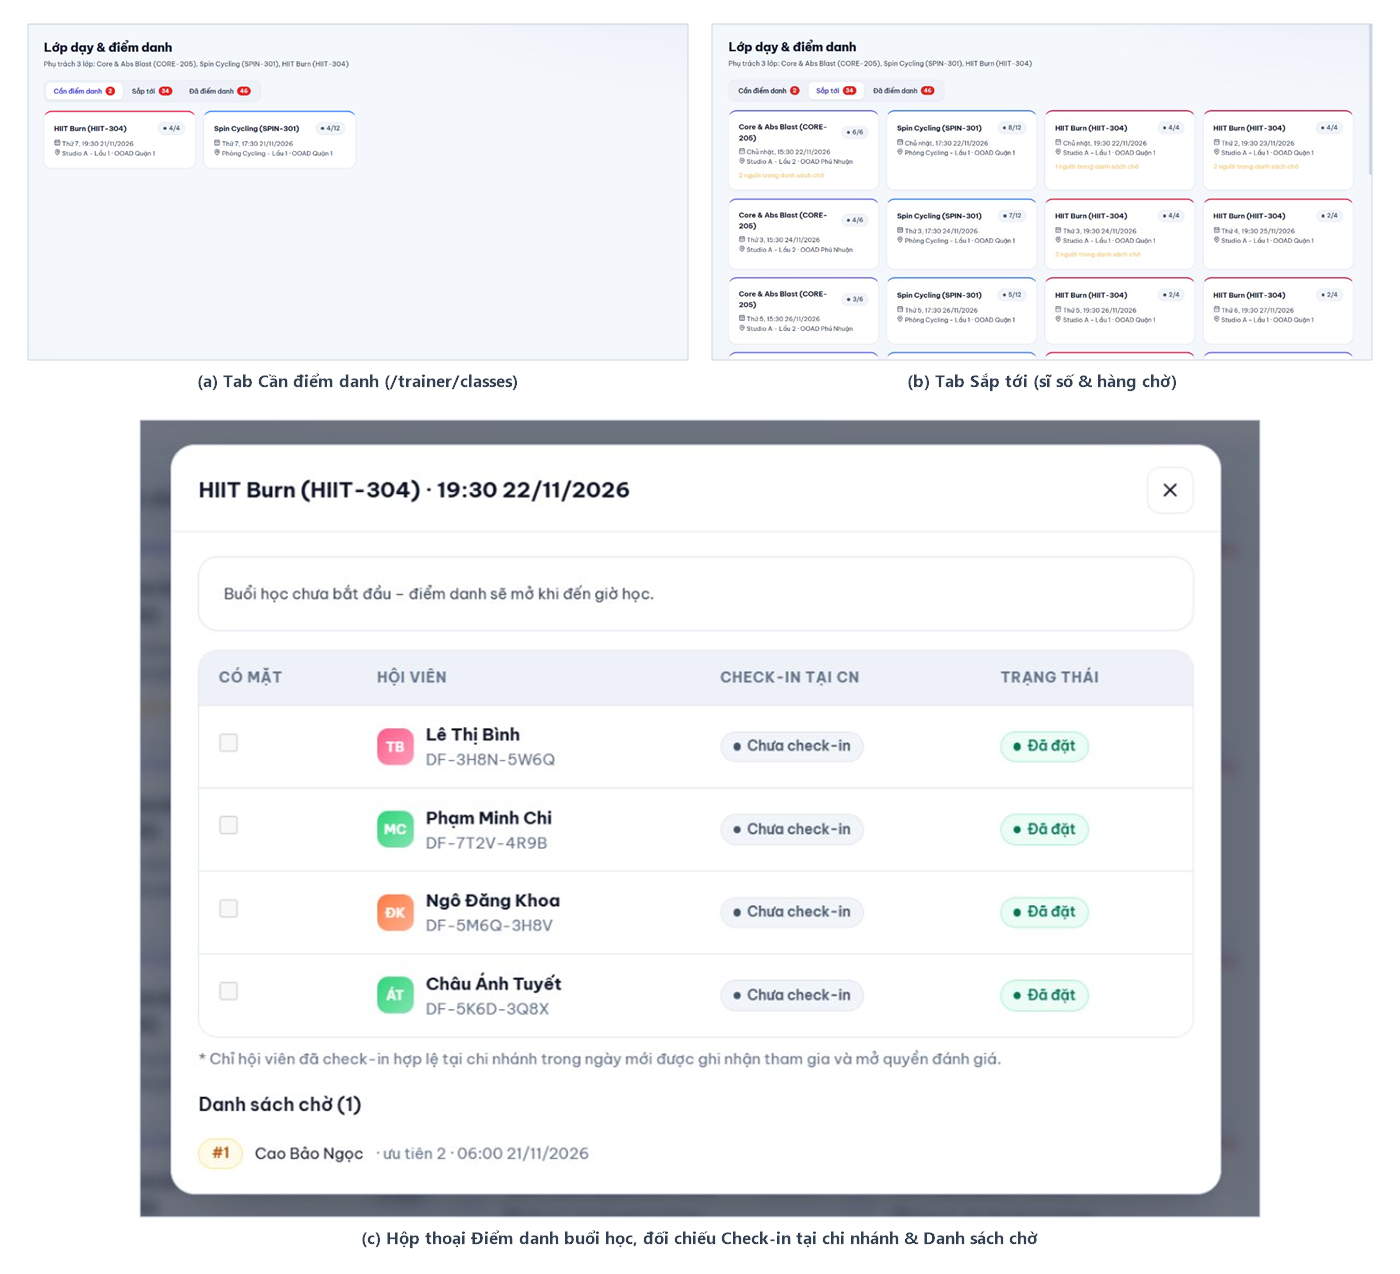
\includegraphics[width=0.96\textwidth]{images/ui_trainer_classes.png}
\caption{Giao diện màn hình Lớp dạy \& Điểm danh của Huấn luyện viên (danh sách buổi dạy và bảng điểm danh)}
\label{fig:ui_trainer_classes}
\end{figure}

\par\medskip\noindent\textbf{Danh sách các thành phần giao diện}\par\smallskip
{\footnotesize
\setlength{\tabcolsep}{2.5pt}
\begin{longtable}{|c|L{2.95cm}|L{1.85cm}|L{2.95cm}|L{2.75cm}|L{1.90cm}|L{2.05cm}|}
\hline
\textbf{STT} & \textbf{Tên} & \textbf{Kiểu} & \textbf{Ý nghĩa} & \textbf{Miền giá trị} & \textbf{Giá trị mặc định} & \textbf{Ghi chú} \\
\hline
\endfirsthead
\hline
\textbf{STT} & \textbf{Tên} & \textbf{Kiểu} & \textbf{Ý nghĩa} & \textbf{Miền giá trị} & \textbf{Giá trị mặc định} & \textbf{Ghi chú} \\
\hline
\endhead
\hline
\endfoot
\hline
\caption{Danh sách các thành phần giao diện -- Màn hình Lớp dạy \& Điểm danh (HLV)} \\
\endlastfoot

\multicolumn{7}{|l|}{\textbf{Phần 1: Màn hình danh sách lớp dạy theo trạng thái (Hình a, b)}} \\ \hline
1 & \texttt{Lbl\_TieuDeHLV} & Label & Tiêu đề màn hình và dòng tóm tắt các lớp HLV đang phụ trách & Chuỗi ký tự & \texttt{"Lớp dạy \& điểm danh"} & Kèm danh sách tên lớp phụ trách \\ \hline
2 & \texttt{Btn\_LamMoiHLV} & Button & Tải lại danh sách các buổi dạy được phân công từ máy chủ & Kích hoạt / Đang tải & \texttt{"Làm mới"} & Hiển thị ở chế độ kết nối API \\ \hline
3 & \texttt{Tab\_TrangThaiBuoi} & Tab Group & Chuyển nhóm buổi dạy theo trạng thái điểm danh & \{\texttt{"Cần điểm danh"}, \texttt{"Sắp tới"}, \texttt{"Đã điểm danh"}\} & \texttt{"Cần điểm danh"} & Hiện badge số lượng trên từng tab \\ \hline
4 & \texttt{Grd\_TheBuoiDay} & Card Grid & Lưới thẻ các buổi dạy thuộc tab hiện tại (màu viền, tên lớp, sĩ số/tỷ lệ có mặt, thời gian, phòng, số người chờ) & Tối đa $30$ thẻ từ \texttt{Class\_Sessions} của HLV & Danh sách thuộc tab \textit{Cần điểm danh} & Nhấn vào thẻ để mở \texttt{Dlg\_DiemDanh} \\ \hline

\multicolumn{7}{|l|}{\textbf{Phần 2: Hộp thoại Điểm danh buổi học \& Đối chiếu Check-in (Hình c)}} \\ \hline
5 & \texttt{Dlg\_DiemDanh} & Modal Dialog & Cửa sổ rộng hiển thị danh sách học viên đăng ký, trạng thái check-in và hàng chờ của buổi dạy & Đóng / Mở & Đóng & Tiêu đề: \texttt{<Tên lớp> \textperiodcentered\ <Giờ Ngày>} \\ \hline
6 & \texttt{Btn\_DongDD} & Button & Nút \texttt{$\times$} (hoặc nút \texttt{Đóng}) thoát hộp thoại điểm danh & Kích hoạt & \texttt{"$\times$"} & Không lưu nếu chưa nhấn xác nhận \\ \hline
7 & \texttt{Pnl\_CanhBaoGio} & Alert Panel & Khung thông báo khi buổi học chưa tới giờ bắt đầu & Hiển thị / Ẩn & Hiện khi \texttt{Start\_At} $>$ hiện tại & Ví dụ: \texttt{"Buổi học chưa bắt đầu -- điểm danh sẽ mở khi đến giờ học."} \\ \hline
8 & \texttt{Tbl\_DanhSachHV} & DataGrid & Bảng $4$ cột (\textit{Có mặt}, \textit{Hội viên}, \textit{Check-in tại CN}, \textit{Trạng thái}) hiển thị danh sách lớp & Vé \texttt{Confirmed}, \texttt{Attended}, \texttt{NoShow} & Tải khi mở \texttt{Dlg\_DiemDanh} & Hiển thị ảnh đại diện viết tắt, họ tên và mã thẻ \\ \hline
9 & \texttt{Chk\_CoMat} & Checkbox & Đánh dấu hội viên có mặt tham gia buổi học trên từng dòng & \{\texttt{True}, \texttt{False}\} & Tự tích sẵn nếu \texttt{Attended} hoặc đã check-in tại CN & Bị khóa khi buổi chưa bắt đầu hoặc đã bị hủy \\ \hline
10 & \texttt{Lbl\_CheckInCN} & Badge & Đối chiếu thời điểm quẹt thẻ check-in tại chi nhánh trong ngày diễn ra buổi học & \{\texttt{"Đã check-in (HH:mm)"}, \texttt{"Chưa check-in"}\} & Truy vấn từ bảng \texttt{Checkins} & Ràng buộc điều kiện xác nhận tham gia \\ \hline
11 & \texttt{Lbl\_TrangThaiHV} & Badge & Trạng thái ghi nhận chuyên cần của học viên & \{\texttt{"Đã đặt"}, \texttt{"Đã tham gia"}, \texttt{"Vắng mặt"}, \texttt{"Đã hủy"}\} & Theo bản ghi \texttt{Bookings} & Tự cập nhật sau khi chốt điểm danh \\ \hline
12 & \texttt{Lbl\_GhiChuCheckIn} & Label & Dòng lưu ý quy định bắt buộc phải check-in tại chi nhánh trong ngày & Chuỗi cố định & Luôn hiển thị dưới bảng & Nhấn mạnh điều kiện mở quyền đánh giá \\ \hline
13 & \texttt{Lst\_HangChoHV} & List View & Danh sách hội viên đang chờ Waitlist của buổi học (thứ tự \texttt{\#k}, tên, gói, mức ưu tiên, giờ đăng ký) & Bản ghi \texttt{Waitlist\_Entries} còn hiệu lực & Ẩn nếu danh sách chờ rỗng & Hiển thị tham chiếu ngay trong hộp thoại \\ \hline
14 & \texttt{Btn\_XacNhanDD} & Button & Lưu kết quả điểm danh (\textit{Xác nhận danh sách tham gia}) cho buổi học & Kích hoạt / Đang lưu / Ẩn & Ẩn nếu buổi chưa bắt đầu hoặc đã hủy & Chốt trạng thái \texttt{Attended} / \texttt{NoShow} \\ \hline

\end{longtable}
}

\par\medskip\noindent\textbf{Danh sách các biến cố}\par\smallskip
{\footnotesize
\setlength{\tabcolsep}{4pt}
\begin{longtable}{|c|L{3.5cm}|L{7.8cm}|L{3.5cm}|}
\hline
\textbf{STT} & \textbf{Điều kiện kích hoạt} & \textbf{Xử lý} & \textbf{Ghi chú} \\
\hline
\endfirsthead
\hline
\textbf{STT} & \textbf{Điều kiện kích hoạt} & \textbf{Xử lý} & \textbf{Ghi chú} \\
\hline
\endhead
\hline
\endfoot
\hline
\caption{Danh sách các biến cố -- Màn hình Lớp dạy \& Điểm danh (HLV)} \\
\endlastfoot

0 & Khởi động màn hình (\texttt{/trainer/classes}) &
Hệ thống truy vấn toàn bộ buổi dạy trong \texttt{Class\_Sessions} được phân công cho HLV đang đăng nhập; tách làm $3$ nhóm (\textit{Cần điểm danh}, \textit{Sắp tới}, \textit{Đã điểm danh}), thống kê tóm tắt danh sách lớp phụ trách lên \texttt{Lbl\_TieuDeHLV} và hiển thị mặc định tab \textit{Cần điểm danh} trên \texttt{Grd\_TheBuoiDay}. &
Chỉ hiển thị các buổi do chính HLV đó phụ trách. \\ \hline

1 & Chọn một tab trên \texttt{Tab\_TrangThaiBuoi} (\textit{Cần điểm danh}, \textit{Sắp tới}, \textit{Đã điểm danh}) &
Đánh dấu tab đang chọn và kết xuất danh sách thẻ buổi dạy tương ứng lên \texttt{Grd\_TheBuoiDay} theo đúng thứ tự thời gian (tăng dần cho \textit{Sắp tới}, giảm dần cho \textit{Cần điểm danh} và \textit{Đã điểm danh}). &
Hiển thị thông báo rỗng nếu tab không có buổi học nào. \\ \hline

2 & Nhấn nút \texttt{Btn\_LamMoiHLV} (\textit{Làm mới}) &
Gọi API đồng bộ lại danh sách buổi dạy, sĩ số hiện tại và số lượng người trong hàng chờ Waitlist mới nhất của HLV rồi cập nhật các tab. &
Chỉ hiện khi kết nối trực tiếp API máy chủ. \\ \hline

3 & Nhấn vào một thẻ buổi dạy bất kỳ trên \texttt{Grd\_TheBuoiDay} &
Mở hộp thoại \texttt{Dlg\_DiemDanh}; tải chi tiết danh sách học viên từ \texttt{Bookings}, đối chiếu lịch sử check-in tại chi nhánh trong ngày từ bảng \texttt{Checkins} và danh sách chờ từ \texttt{Waitlist\_Entries}; tự động đánh dấu sẵn \texttt{Chk\_CoMat} với các học viên đã check-in hợp lệ hoặc đã điểm danh. Nếu buổi chưa đến giờ bắt đầu, bật \texttt{Pnl\_CanhBaoGio}, khóa \texttt{Chk\_CoMat} và ẩn \texttt{Btn\_XacNhanDD}. &
Giúp HLV rà soát nhanh người đã check-in tại quầy lễ tân. \\ \hline

4 & Chọn hoặc bỏ chọn ô \texttt{Chk\_CoMat} của một học viên trong \texttt{Tbl\_DanhSachHV} &
Thêm hoặc xóa mã vé/hội viên khỏi mảng danh sách được chọn có mặt (\texttt{selectedIds}) trong phiên điểm danh đang mở. &
Chỉ thao tác được khi buổi học đã đến giờ bắt đầu và chưa bị hủy. \\ \hline

5 & Nhấn nút \texttt{Btn\_XacNhanDD} (\textit{Xác nhận danh sách tham gia}) &
Gửi danh sách \texttt{selectedIds} xuống hệ thống xử lý: kiểm tra đối chiếu lại với bảng \texttt{Checkins} tại chi nhánh trong ngày; các học viên được đánh dấu \textbf{và} đã check-in hợp lệ được chuyển sang \texttt{Attended} (đồng thời mở quyền đánh giá); các trường hợp còn lại (hoặc chưa check-in hợp lệ) bị ghi nhận \texttt{NoShow}; đánh dấu buổi học đã xác nhận điểm danh, thông báo kết quả (kèm số lượng bị từ chối nếu chưa check-in), đóng \texttt{Dlg\_DiemDanh} và tải lại lưới thẻ. &
Đảm bảo không thể điểm danh khống cho hội viên không đến chi nhánh. \\ \hline

6 & Nhấn nút \texttt{Btn\_DongDD} (\texttt{$\times$} hoặc \texttt{Đóng}) của \texttt{Dlg\_DiemDanh} &
Hủy bỏ các thay đổi tạm thời chưa lưu, đóng hộp thoại \texttt{Dlg\_DiemDanh} và quay lại màn hình danh sách thẻ buổi dạy. &
Dữ liệu điểm danh trước đó trên máy chủ vẫn được giữ nguyên. \\ \hline

\end{longtable}
}


\subsubsection{Màn hình Quản lý Lớp học Nhóm (Quản trị viên)}
Màn hình \textbf{Quản lý Lớp học Nhóm} (đường dẫn \texttt{/admin/classes}) cung cấp cho \textbf{Quản trị viên (Admin)} bộ công cụ tập trung để khởi tạo và bảo trì danh mục lớp học định kỳ, theo dõi lịch các buổi học theo từng tuần, tìm kiếm/lọc theo chi nhánh -- bộ môn -- trạng thái, đồng thời đổi lịch (có kiểm tra xung đột phòng tập và HLV) hoặc hủy từng buổi học cụ thể khi phát sinh sự cố.

Giao diện được bố cục thành 2 tab làm việc rõ ràng như minh họa ở Hình~\ref{fig:ui_admin_classes}:
\begin{itemize}
    \item \textbf{Hình (a) -- Tab Danh mục lớp học định kỳ:} Hiển thị ô tìm kiếm nhanh, bộ lọc chi nhánh và lưới thẻ các lớp đang hoạt động với đầy đủ thông tin HLV, phòng, khung giờ lặp, sĩ số tối đa và các nút \texttt{Sửa}, \texttt{Hủy lớp}, \texttt{Xem lịch tuần}.
    \item \textbf{Hình (b) -- Tab Lịch buổi học theo tuần:} Tích hợp thanh điều hướng tuần, bộ lọc lớp/trạng thái, dải chip bộ môn và bảng $6$ cột liệt kê từng buổi học cùng hai thao tác xử lý nhanh \texttt{Đổi lịch} và \texttt{Hủy buổi}.
\end{itemize}

\begin{figure}[H]
\centering
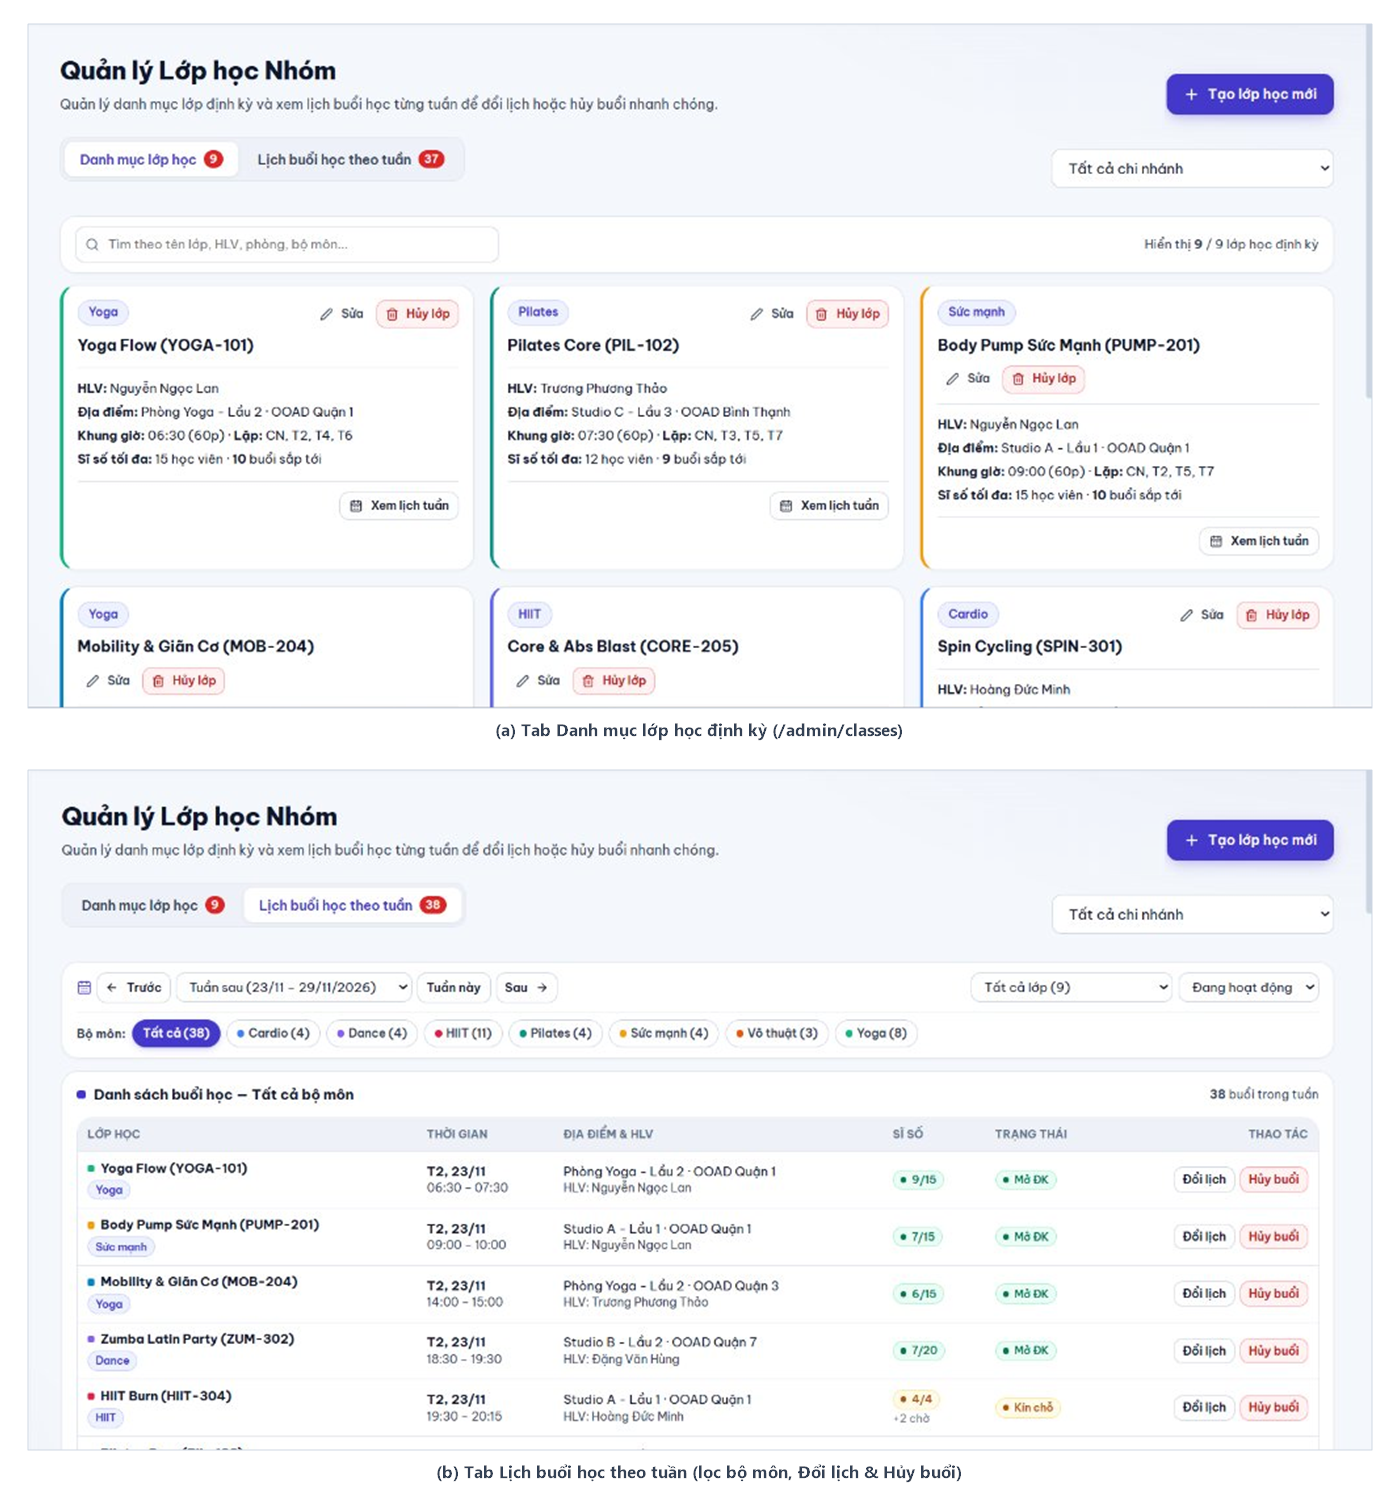
\includegraphics[width=0.96\textwidth]{images/ui_admin_classes.png}
\caption{Giao diện màn hình Quản lý Lớp học Nhóm dành cho Quản trị viên (Danh mục lớp học và Lịch buổi học theo tuần)}
\label{fig:ui_admin_classes}
\end{figure}

\par\medskip\noindent\textbf{Danh sách các thành phần giao diện}\par\smallskip
{\footnotesize
\setlength{\tabcolsep}{2.5pt}
\begin{longtable}{|c|L{2.95cm}|L{1.85cm}|L{2.95cm}|L{2.75cm}|L{1.90cm}|L{2.05cm}|}
\hline
\textbf{STT} & \textbf{Tên} & \textbf{Kiểu} & \textbf{Ý nghĩa} & \textbf{Miền giá trị} & \textbf{Giá trị mặc định} & \textbf{Ghi chú} \\
\hline
\endfirsthead
\hline
\textbf{STT} & \textbf{Tên} & \textbf{Kiểu} & \textbf{Ý nghĩa} & \textbf{Miền giá trị} & \textbf{Giá trị mặc định} & \textbf{Ghi chú} \\
\hline
\endhead
\hline
\endfoot
\hline
\caption{Danh sách các thành phần giao diện -- Màn hình Quản lý Lớp học Nhóm (Admin)} \\
\endlastfoot

\multicolumn{7}{|l|}{\textbf{Phần 1: Thanh tiêu đề, Tab chính \& Bộ lọc chi nhánh chung}} \\ \hline
1 & \texttt{Lbl\_TieuDeAdmin} & Label & Tiêu đề màn hình và mô tả ngắn phạm vi quản lý lớp học nhóm & Chuỗi ký tự & \texttt{"Quản lý Lớp học Nhóm"} & Chỉ đọc \\ \hline
2 & \texttt{Btn\_LamMoiAdmin} & Button & Đồng bộ lại danh mục lớp, chi nhánh, HLV và lịch buổi học tuần từ API & Kích hoạt / Đang tải & \texttt{"Làm mới"} & Hiển thị ở chế độ kết nối API \\ \hline
3 & \texttt{Btn\_TaoLopMoi} & Button & Mở hộp thoại tạo một lớp học nhóm định kỳ mới & Kích hoạt & \texttt{"+ Tạo lớp học mới"} & Mở \texttt{Dlg\_FormLop} ở chế độ tạo mới \\ \hline
4 & \texttt{Tab\_QuanLyLop} & Tab Group & Chuyển giữa quản lý danh mục lớp định kỳ và danh sách buổi học theo tuần & \{\texttt{"Danh mục lớp học"}, \texttt{"Lịch buổi học theo tuần"}\} & \texttt{"Danh mục lớp học"} & Hiện số lớp và số buổi hoạt động trong tuần \\ \hline
5 & \texttt{Cbo\_ChiNhanhAdmin} & ComboBox & Lọc dữ liệu cả 2 tab theo chi nhánh tổ chức & \texttt{"Tất cả chi nhánh"} + các chi nhánh từ \texttt{Branches} & \texttt{"Tất cả chi nhánh"} & Khi đổi chi nhánh tự đặt bộ lọc lớp về tất cả \\ \hline

\multicolumn{7}{|l|}{\textbf{Phần 2: Tab Danh mục lớp học định kỳ (Hình a)}} \\ \hline
6 & \texttt{Txt\_TimKiemLop} & Textbox & Nhập từ khóa tìm kiếm theo tên lớp, HLV, phòng tập, bộ môn hoặc chi nhánh & Chuỗi văn bản & Rỗng & Lọc tức thời danh mục thẻ lớp \\ \hline
7 & \texttt{Lbl\_DemLop} & Label & Hiển thị tỷ lệ số lớp đang khớp từ khóa trên tổng số lớp & \texttt{Hiển thị M / N lớp học định kỳ} & \texttt{N / N} & Cập nhật ngay khi tìm kiếm hoặc lọc chi nhánh \\ \hline
8 & \texttt{Grd\_DanhMucLop} & Card Grid & Lưới $3$ cột thẻ lớp định kỳ: badge bộ môn, tên lớp, HLV, địa điểm, khung giờ lặp, sĩ số tối đa, số buổi sắp tới & Các lớp hoạt động trong \texttt{GymClass} & Toàn bộ lớp định kỳ đang mở & Có dải màu phân biệt bên cạnh trái mỗi thẻ \\ \hline
9 & \texttt{Btn\_SuaHuyLop} & Button Pair & Cặp nút \texttt{Sửa} (chỉnh thông tin định kỳ) và \texttt{Hủy lớp} (ngừng hoạt động lớp) trên thẻ & Kích hoạt / Vô hiệu khi đang lưu & Hiển thị trên từng thẻ lớp & \texttt{Hủy lớp} tự hủy các buổi tương lai và hoàn lượt \\ \hline
10 & \texttt{Btn\_XemLichTuan} & Button Pair & Nút \texttt{Xem lịch tuần} (chuyển sang Tab 2 và lọc đúng lớp đó) và \texttt{Sinh +2 tuần} (API) & Kích hoạt & Hiển thị ở chân thẻ lớp & Hỗ trợ sinh tiếp lịch định kỳ nhanh \\ \hline

\multicolumn{7}{|l|}{\textbf{Phần 3: Tab Lịch buổi học theo tuần (Hình b)}} \\ \hline
11 & \texttt{Grp\_ChonTuanAdmin} & Control Group & Cụm nút \texttt{$\leftarrow$ Trước}, \texttt{ComboBox} chọn tuần (\texttt{Tuần -2} đến \texttt{+6}), nút \texttt{Tuần này}, \texttt{Sau $\rightarrow$} & Chọn tuần Thứ Hai -- Chủ Nhật & \texttt{Tuần này} (\texttt{weekIdx = 0}) & Nút \texttt{Tuần này} vô hiệu khi đang ở tuần gốc \\ \hline
12 & \texttt{Cbo\_LocLop} & ComboBox & Lọc buổi học theo từng lớp định kỳ cụ thể (kèm nút \texttt{Bỏ lọc} khi đang chọn riêng 1 lớp) & \texttt{"Tất cả lớp (N)"} + danh sách lớp & \texttt{"Tất cả lớp"} & Tự động cập nhật theo chi nhánh \\ \hline
13 & \texttt{Cbo\_TrangThaiBuoi} & ComboBox & Lọc buổi học theo tình trạng vận hành & \{\texttt{"Đang hoạt động"}, \texttt{"Sắp diễn ra"}, \texttt{"Tất cả"}, \texttt{"Đã hủy"}\} & \texttt{"Đang hoạt động"} & Ẩn các buổi đã hủy ở chế độ mặc định \\ \hline
14 & \texttt{Chip\_BoMonAdmin} & Chip Button & Nhóm nút lọc bộ môn kèm tổng số buổi tương ứng trong tuần & \texttt{Tất cả (N)} và các bộ môn phát sinh (\texttt{Cardio}, \texttt{Dance}, \texttt{HIIT}, ...) & \texttt{"Tất cả"} & Cập nhật số lượng động theo các bộ lọc trên \\ \hline
15 & \texttt{Grd\_BuoiHocAdmin} & DataGrid & Bảng $6$ cột (\textit{Lớp học}, \textit{Thời gian}, \textit{Địa điểm \& HLV}, \textit{Sĩ số}, \textit{Trạng thái}, \textit{Thao tác}) kèm nhãn tổng số buổi & Bản ghi từ \texttt{Class\_Sessions} sắp tăng dần theo \texttt{Start\_At} & Toàn bộ buổi hợp lệ trong tuần & Cột \textit{Trạng thái}: \texttt{Mở ĐK}, \texttt{Kín chỗ}, \texttt{Đã hủy}, \texttt{Hoàn thành}, \texttt{Đã qua} \\ \hline
16 & \texttt{Btn\_DoiHuyBuoi} & Button Pair & Cặp nút \texttt{Đổi lịch} và \texttt{Hủy buổi} trên các dòng buổi học chưa diễn ra & Hiển thị khi buổi chưa bắt đầu và chưa hủy/xong & Hiện dấu \texttt{"--"} với buổi đã qua/hủy & Mở \texttt{Dlg\_DoiLich} hoặc \texttt{Dlg\_HuyBuoi} \\ \hline

\multicolumn{7}{|l|}{\textbf{Phần 4: Các hộp thoại nghiệp vụ tạo/sửa lớp, đổi lịch \& hủy buổi}} \\ \hline
17 & \texttt{Dlg\_FormLop} & Modal Dialog & Form nhập/sửa lớp định kỳ: tên, chi nhánh, phòng, HLV, giờ, thời lượng, sĩ số, ngày lặp, màu/số tuần sinh trước & Hợp lệ khi không trùng phòng và trùng lịch HLV & Đóng & Tự động kiểm tra ràng buộc xung đột lịch \\ \hline
18 & \texttt{Dlg\_DoiLich} & Modal Dialog & Hộp thoại đổi ngày, giờ bắt đầu, phòng hoặc HLV thay thế cho một buổi học đơn lẻ & Chỉ lưu khi không trùng phòng tập và không trùng lịch dạy HLV trong cùng khung giờ & Đóng & Cảnh báo xung đột trực tiếp trước khi lưu \\ \hline
19 & \texttt{Dlg\_HuyBuoi} & Confirm Dialog & Hộp thoại nhập lý do hủy buổi học và xác nhận thực thi hủy buổi & Chuỗi lý do hủy (có lý do mặc định) & Đóng & Hoàn lượt cho học viên và gửi thông báo \\ \hline

\end{longtable}
}

\par\medskip\noindent\textbf{Danh sách các biến cố}\par\smallskip
{\footnotesize
\setlength{\tabcolsep}{4pt}
\begin{longtable}{|c|L{3.5cm}|L{7.8cm}|L{3.5cm}|}
\hline
\textbf{STT} & \textbf{Điều kiện kích hoạt} & \textbf{Xử lý} & \textbf{Ghi chú} \\
\hline
\endfirsthead
\hline
\textbf{STT} & \textbf{Điều kiện kích hoạt} & \textbf{Xử lý} & \textbf{Ghi chú} \\
\hline
\endhead
\hline
\endfoot
\hline
\caption{Danh sách các biến cố -- Màn hình Quản lý Lớp học Nhóm (Admin)} \\
\endlastfoot

0 & Khởi động màn hình (\texttt{/admin/classes}) &
Hệ thống tải danh sách lớp định kỳ từ \texttt{GymClass}, danh sách chi nhánh, danh sách HLV và các buổi học trong tuần hiện tại từ \texttt{Class\_Sessions}; mặc định mở tab \textit{Danh mục lớp học} (\texttt{Grd\_DanhMucLop}) và hiển thị đếm số lượng trên tiêu đề các tab. &
Dữ liệu cả hai tab sẵn sàng khi Admin chuyển qua lại. \\ \hline

1 & Chọn giá trị trên \texttt{Cbo\_ChiNhanhAdmin} hoặc chuyển tab trên \texttt{Tab\_QuanLyLop} &
Lọc lại danh sách lớp định kỳ ở Tab 1 và danh sách buổi học tuần ở Tab 2 theo đúng chi nhánh được chọn; đặt lại \texttt{Cbo\_LocLop} về \texttt{"Tất cả lớp"} nếu lớp đang lọc không thuộc chi nhánh mới. Chuyển vùng hiển thị tương ứng với tab được chọn. &
Giúp Admin theo dõi riêng từng cơ sở chi nhánh. \\ \hline

2 & Nhập từ khóa vào \texttt{Txt\_TimKiemLop} &
Lọc tức thời các thẻ lớp trong \texttt{Grd\_DanhMucLop} khớp theo tên lớp, tên HLV, tên phòng, bộ môn hoặc chi nhánh và cập nhật bộ đếm \texttt{Lbl\_DemLop}. &
Nếu không có lớp phù hợp, hiển thị gợi ý xóa từ khóa hoặc tạo mới. \\ \hline

3 & Nhấn \texttt{Btn\_TaoLopMoi} hoặc nút \texttt{Sửa} trên \texttt{Btn\_SuaHuyLop} rồi lưu \texttt{Dlg\_FormLop} &
Mở \texttt{Dlg\_FormLop} với dữ liệu trống hoặc dữ liệu lớp đang chọn; khi Admin nhấn \textit{Lưu lớp học}, hệ thống kiểm tra dữ liệu bắt buộc, kiểm tra trùng phòng tập và trùng lịch HLV theo khung giờ và các ngày lặp trong tuần. Nếu hợp lệ, lưu vào \texttt{GymClass}, sinh các buổi học tương ứng vào \texttt{Class\_Sessions}, thông báo cho HLV và làm mới dữ liệu. &
Báo lỗi chi tiết ngay trên hộp thoại nếu bị trùng phòng hoặc trùng HLV. \\ \hline

4 & Nhấn nút \texttt{Hủy lớp} trên \texttt{Btn\_SuaHuyLop} &
Hiển thị hộp thoại xác nhận ngừng lớp; nếu đồng ý, đánh dấu ngừng hoạt động lớp trong \texttt{GymClass}, tự động hủy toàn bộ buổi học tương lai chưa diễn ra thuộc lớp đó và hoàn lại lượt đặt cho các học viên đã đăng ký. &
Bảo toàn lịch sử các buổi đã diễn ra trước thời điểm hủy. \\ \hline

5 & Nhấn \texttt{Xem lịch tuần} hoặc \texttt{Sinh +2 tuần} trên \texttt{Btn\_XemLichTuan} &
Với \texttt{Xem lịch tuần}: gán \texttt{Cbo\_LocLop} về mã lớp tương ứng và tự động chuyển sang Tab \textit{Lịch buổi học theo tuần}. Với \texttt{Sinh +2 tuần}: gọi API sinh bổ sung các buổi định kỳ $2$ tuần tiếp theo cho lớp và cập nhật bộ đếm buổi sắp tới. &
Tiện theo dõi lịch chi tiết của riêng một lớp sau khi tạo/chỉnh sửa. \\ \hline

6 & Điều hướng tuần trên \texttt{Grp\_ChonTuanAdmin} (\texttt{Trước}, chọn tuần, \texttt{Tuần này}, \texttt{Sau}) &
Cập nhật chỉ số tuần \texttt{weekIdx}, tính lại $7$ ngày Thứ Hai -- Chủ Nhật, truy vấn các buổi học thuộc tuần mới từ \texttt{Class\_Sessions} và làm mới bảng \texttt{Grd\_BuoiHocAdmin} cùng bộ đếm \texttt{Chip\_BoMonAdmin}. &
Cho phép quản lý lịch từ $2$ tuần trước tới $6$ tuần sau. \\ \hline

7 & Thay đổi bộ lọc \texttt{Cbo\_LocLop}, \texttt{Cbo\_TrangThaiBuoi} hoặc chọn bộ môn trên \texttt{Chip\_BoMonAdmin} &
Lọc lại các buổi học của tuần đang chọn theo lớp (hoặc nhấn \textit{Bỏ lọc} để về tất cả), trạng thái vận hành và bộ môn tương ứng; sắp xếp tăng dần theo \texttt{Start\_At} và kết xuất lên \texttt{Grd\_BuoiHocAdmin}. &
Tự đưa \texttt{Chip\_BoMonAdmin} về \texttt{"Tất cả"} nếu bộ lọc mới không còn buổi của bộ môn cũ. \\ \hline

8 & Nhấn \texttt{Đổi lịch} trên \texttt{Btn\_DoiHuyBuoi} và lưu trên \texttt{Dlg\_DoiLich} &
Mở \texttt{Dlg\_DoiLich} cho buổi học được chọn để sửa ngày, giờ bắt đầu, phòng tập hoặc HLV. Khi xác nhận lưu, hệ thống kiểm tra quy tắc: tránh trùng lịch nếu có lớp khác mở cùng thời điểm nhưng phải đảm bảo tối đa $1$ lớp / $1$ HLV / $1$ phòng trong cùng khung giờ. Nếu hợp lệ, cập nhật \texttt{Class\_Sessions}, thông báo tới các học viên đã đặt và HLV liên quan. &
Cảnh báo xung đột trực tiếp trên hộp thoại trước khi cho phép xác nhận. \\ \hline

9 & Nhấn \texttt{Hủy buổi} trên \texttt{Btn\_DoiHuyBuoi} và xác nhận trên \texttt{Dlg\_HuyBuoi} &
Mở hộp thoại nhập lý do hủy buổi; khi xác nhận, cập nhật trạng thái buổi sang \texttt{CANCELLED}, hoàn lại lượt đặt cho tất cả học viên đã đặt (\texttt{Confirmed}), giải phóng hàng chờ \texttt{Waitlist\_Entries} và gửi thông báo cho học viên cùng HLV phụ trách. &
Các buổi đã hủy không còn cho phép đổi lịch hoặc hủy lại. \\ \hline

10 & Nhấn nút \texttt{Btn\_LamMoiAdmin} (\textit{Làm mới}) &
Gọi đồng thời API tải lại danh mục lớp, danh sách chi nhánh, danh sách HLV và buổi học trong tuần đang xem để cập nhật toàn bộ giao diện Admin. &
Chỉ hiển thị khi kết nối trực tiếp API máy chủ. \\ \hline

\end{longtable}
}


\newpage
\subsection{Phân hệ PT 1-kèm-1, Tiến độ thể hình \& Đánh giá}
Phân hệ \textbf{PT 1-kèm-1, Tiến độ thể hình \& Đánh giá} kết nối trực tiếp quy trình đặt lịch huấn luyện cá nhân và theo dõi chỉ số cơ thể của \textbf{Hội viên} với công tác thiết lập khung giờ rảnh, phê duyệt lịch hẹn và tổng hợp phản hồi đánh giá của \textbf{Huấn luyện viên (PT)}.

% -------------------------------------------------------------------------
% 6.5.1 TRANG CHỦ HỘI VIÊN (/member)
% -------------------------------------------------------------------------
\subsubsection{Màn hình Trang chủ Hội viên (Hội viên)}
Màn hình \textbf{Trang chủ Hội viên} (đường dẫn \texttt{/member}) là không gian làm việc trung tâm của \textbf{Hội viên}, hiển thị thẻ chào mừng kèm thông tin gói tập hiệu lực, 4 thẻ chỉ số KPI cá nhân (số buổi PT còn lại, lượt đến phòng 30 ngày, tổng giờ tập, số buổi đã hoàn thành), danh sách lịch tập sắp tới và biểu đồ biến thiên cân nặng thu gọn.

\begin{figure}[H]
\centering
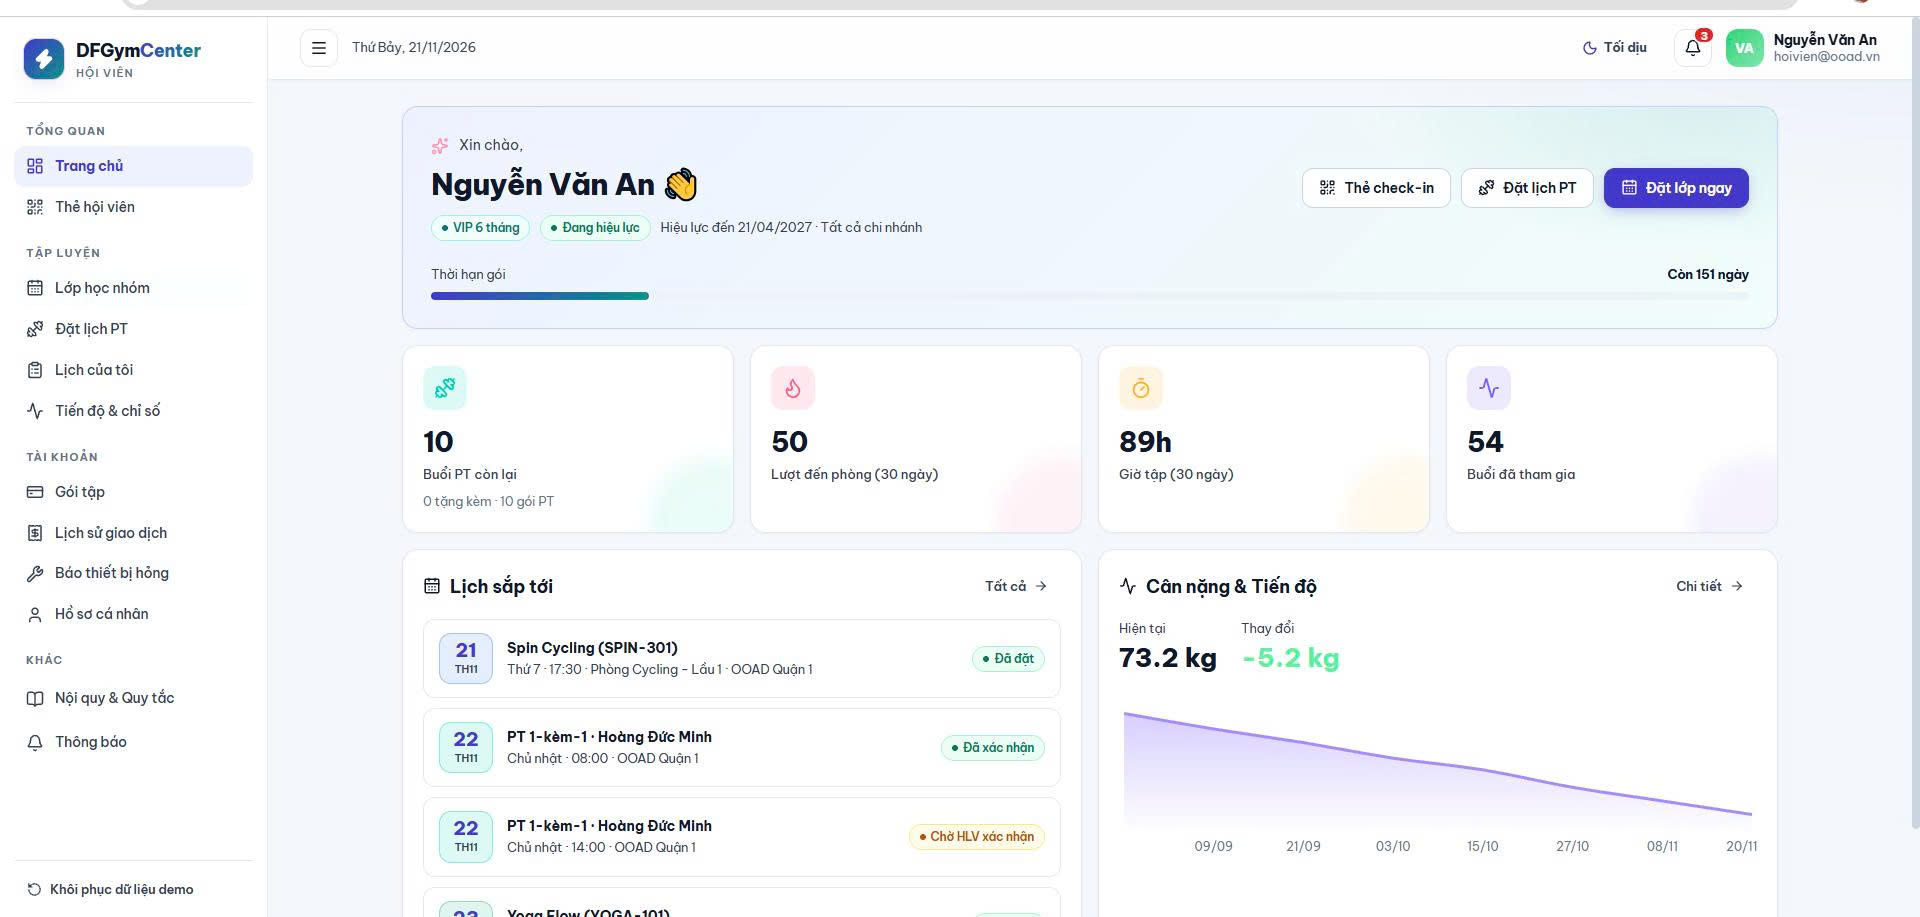
\includegraphics[width=0.92\textwidth]{images/ui_shunei/sh01_member_home.jpg}
\caption{Giao diện màn hình Trang chủ Hội viên (\texttt{/member})}
\label{fig:sh-member-home}
\end{figure}

\par\medskip\noindent\textbf{Danh sách các thành phần giao diện}\par\smallskip
{\footnotesize
\setlength{\tabcolsep}{2.5pt}
\begin{longtable}{|c|L{2.95cm}|L{1.85cm}|L{2.95cm}|L{2.75cm}|L{1.90cm}|L{2.05cm}|}
\hline
\textbf{STT} & \textbf{Tên} & \textbf{Kiểu} & \textbf{Ý nghĩa} & \textbf{Miền giá trị} & \textbf{Giá trị mặc định} & \textbf{Ghi chú} \\
\hline
\endfirsthead
\hline
\textbf{STT} & \textbf{Tên} & \textbf{Kiểu} & \textbf{Ý nghĩa} & \textbf{Miền giá trị} & \textbf{Giá trị mặc định} & \textbf{Ghi chú} \\
\hline
\endhead
\hline
\endfoot
\hline
\caption{Danh sách các thành phần giao diện -- Màn hình Trang chủ Hội viên} \\
\endlastfoot
1 & \texttt{Card\_GoiHoiVien} & Card Panel & Khối Hero Card hiển thị gói tập hiện hành, thời hạn, số ngày còn lại và các nút tác vụ nhanh & Thông tin từ \texttt{Memberships} & Gói đang hiệu lực & Kèm nút \textit{Thẻ check-in}, \textit{Đặt lịch PT}, \textit{Đặt lớp} \\ \hline
2 & \texttt{Stat\_BuoiPT} & StatCard & Thẻ KPI hiển thị tổng số buổi PT 1-kèm-1 khả dụng (tách buổi tặng kèm và buổi gói) & Số nguyên $\ge 0$ & $0$ & Đi kèm 3 thẻ KPI thống kê tập luyện \\ \hline
3 & \texttt{Btn\_DatLichPT} & Button & Nút điều hướng nhanh sang trang đặt lịch huấn luyện viên cá nhân & Kích hoạt & \texttt{"Đặt lịch PT"} & Mở màn hình \texttt{/member/pt} \\ \hline
4 & \texttt{Lst\_LichSapToi} & List View & Danh sách các buổi lớp học nhóm và ca PT 1-kèm-1 sắp diễn ra & Bản ghi từ \texttt{Bookings} & Sắp tăng dần theo giờ & Kèm nút \textit{Xem tất cả lịch} \\* \hline
5 & \texttt{Chart\_\hspace{0pt}CanNangMini} & Chart & Biểu đồ diện tích thu gọn thể hiện biến thiên cân nặng qua các mốc đo & Dữ liệu từ \texttt{Body\_Metrics} & Các mốc đo gần nhất & Có nút \textit{Chi tiết} sang \texttt{/member/\hspace{0pt}progress} \\ \hline
\end{longtable}
}

\par\medskip\noindent\textbf{Danh sách các biến cố}\par\smallskip
{\footnotesize
\setlength{\tabcolsep}{4pt}
\begin{longtable}{|c|L{3.5cm}|L{7.8cm}|L{3.5cm}|}
\hline
\textbf{STT} & \textbf{Điều kiện kích hoạt} & \textbf{Xử lý} & \textbf{Ghi chú} \\
\hline
\endfirsthead
\hline
\textbf{STT} & \textbf{Điều kiện kích hoạt} & \textbf{Xử lý} & \textbf{Ghi chú} \\
\hline
\endhead
\hline
\endfoot
\hline
\caption{Danh sách các biến cố -- Màn hình Trang chủ Hội viên} \\
\endlastfoot
0 & Khởi động màn hình (\texttt{/member}) & Gọi đồng thời các API \texttt{GET /api/trainers/pt-balance} lấy số dư buổi PT, \texttt{GET /api/trainers/pt-bookings/me} tải lịch hẹn PT và \texttt{GET /api/body-measurements/me} tải lịch sử cân nặng để kết xuất thẻ KPI, lịch sắp tới và biểu đồ mini. & Nạp song song bằng \texttt{Promise.allSettled}. \\ \hline
1 & Nhấn nút \texttt{Btn\_DatLichPT} (\textit{Đặt lịch PT}) & Điều hướng người dùng sang màn hình quy trình đặt lịch PT 1-kèm-1 (\texttt{/member/pt}). & Thao tác truy cập nhanh. \\ \hline
2 & Nhấn nút \textit{Chi tiết} tại khối biểu đồ cân nặng & Điều hướng người dùng sang màn hình chi tiết tiến độ thể hình và chỉ số InBody (\texttt{/member/progress}). & Mở toàn bộ lịch sử và biểu đồ mốc đo InBody. \\* \hline
3 & Nhấn nút \textit{Xem tất cả lịch} tại danh sách lịch & Điều hướng người dùng sang màn hình quản lý thời khóa biểu và lịch sử đặt chỗ (\texttt{/member/bookings}). & Xem đầy đủ lịch lớp nhóm và PT. \\ \hline
\end{longtable}
}

% -------------------------------------------------------------------------
% 6.5.2 ĐẶT LỊCH PT 1-KÈM-1 (/member/pt)
% -------------------------------------------------------------------------
\subsubsection{Màn hình Đặt lịch Huấn luyện viên cá nhân (Hội viên)}
Màn hình \textbf{Đặt lịch Huấn luyện viên cá nhân} (đường dẫn \texttt{/member/pt}) cung cấp cho \textbf{Hội viên} quy trình 3 bước trực quan: chọn Huấn luyện viên theo tên/chuyên môn/chi nhánh, chọn ngày và khung giờ rảnh theo ca Sáng -- Chiều -- Tối, sau đó nhập mục tiêu buổi tập và gửi yêu cầu đặt lịch (\texttt{PENDING}).

\begin{figure}[H]
\centering
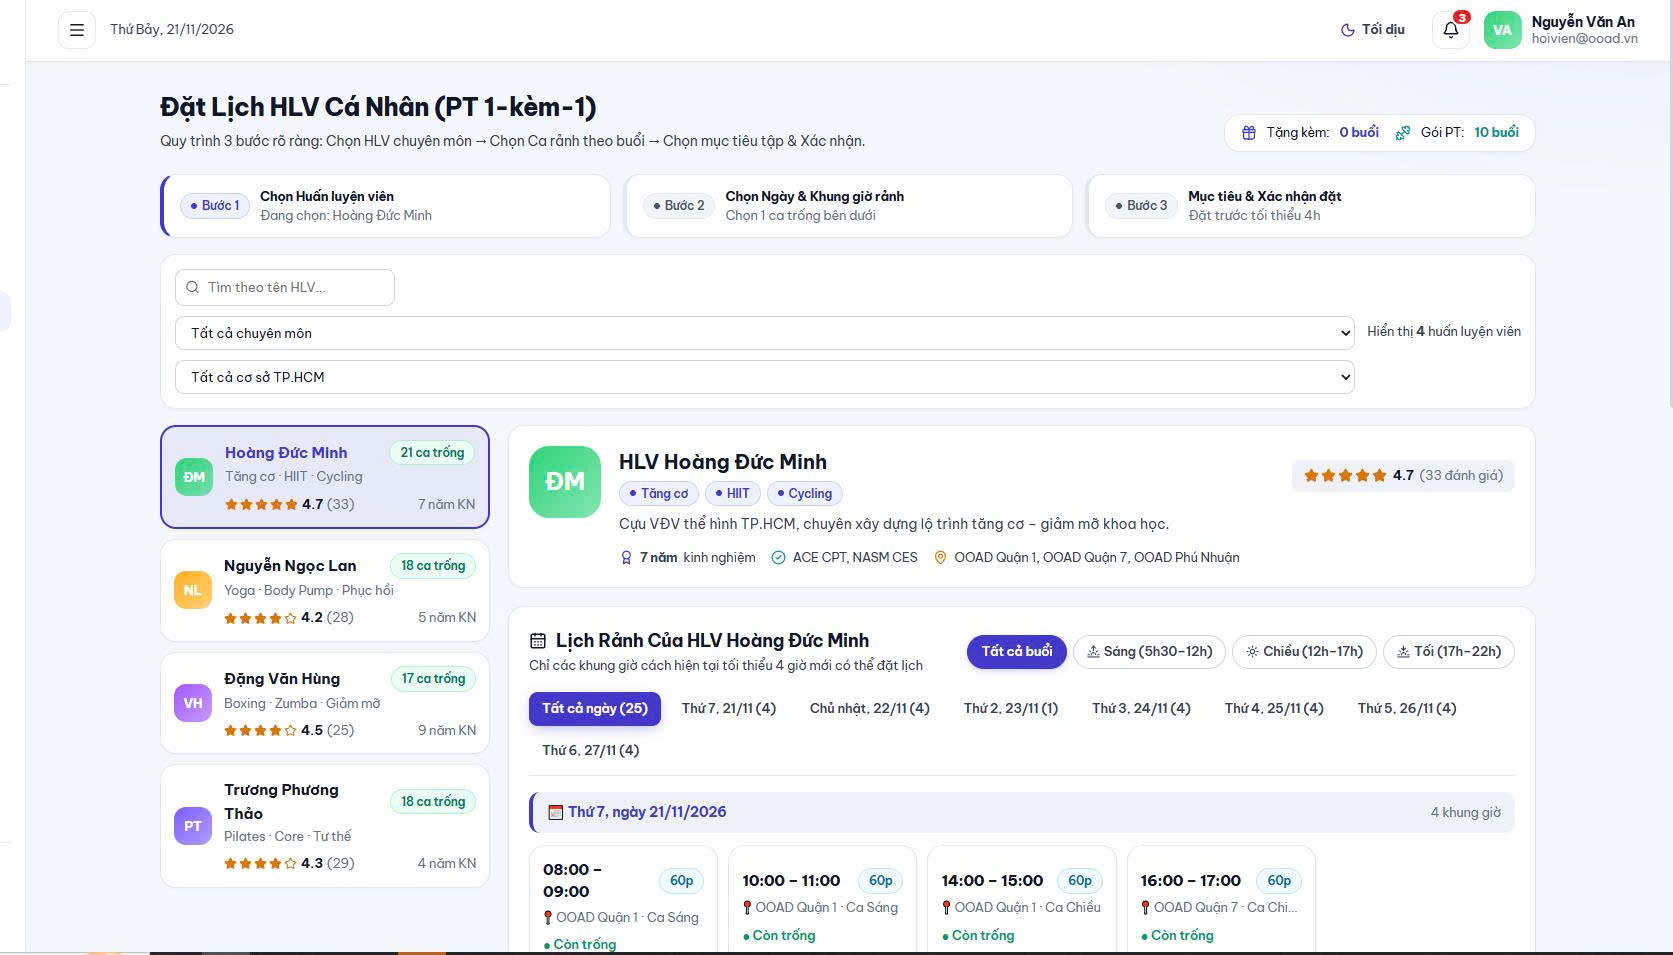
\includegraphics[width=0.92\textwidth]{images/ui_shunei/sh02_member_pt.jpg}
\caption{Giao diện màn hình Đặt lịch Huấn luyện viên cá nhân (\texttt{/member/pt})}
\label{fig:sh-member-pt}
\end{figure}

\par\medskip\noindent\textbf{Danh sách các thành phần giao diện}\par\smallskip
{\footnotesize
\setlength{\tabcolsep}{2.5pt}
\begin{longtable}{|c|L{2.95cm}|L{1.85cm}|L{2.95cm}|L{2.75cm}|L{1.90cm}|L{2.05cm}|}
\hline
\textbf{STT} & \textbf{Tên} & \textbf{Kiểu} & \textbf{Ý nghĩa} & \textbf{Miền giá trị} & \textbf{Giá trị mặc định} & \textbf{Ghi chú} \\
\hline
\endfirsthead
\hline
\textbf{STT} & \textbf{Tên} & \textbf{Kiểu} & \textbf{Ý nghĩa} & \textbf{Miền giá trị} & \textbf{Giá trị mặc định} & \textbf{Ghi chú} \\
\hline
\endhead
\hline
\endfoot
\hline
\caption{Danh sách các thành phần giao diện -- Màn hình Đặt lịch PT 1-kèm-1} \\
\endlastfoot
1 & \texttt{Txt\_TimHLV} & Textbox & Tìm kiếm Huấn luyện viên theo từ khóa họ tên & Chuỗi ký tự & Rỗng & Lọc tức thời danh sách bên trái \\ \hline
2 & \texttt{Cbo\_ChuyenMon} & ComboBox & Lọc danh sách HLV theo lĩnh vực chuyên môn & Danh mục chuyên môn & \texttt{"Tất cả chuyên môn"} & Kết hợp cùng lọc chi nhánh \\ \hline
3 & \texttt{Cbo\_ChiNhanh} & ComboBox & Lọc HLV theo chi nhánh phòng tập công tác & Danh sách từ \texttt{Branches} & \texttt{"Tất cả cơ sở TP.HCM"} & Chỉ hiện HLV thuộc chi nhánh \\ \hline
4 & \texttt{Lst\_HLV} & List View & Danh sách thẻ HLV gồm ảnh, chuyên môn, thâm niên, điểm sao và số ca trống & Danh sách HLV hoạt động & Toàn bộ HLV khả dụng & Nhấp chọn để xem lịch rảnh \\ \hline
5 & \texttt{Grd\_CaRanh} & Card Grid & Lưới khung giờ rảnh theo ngày và buổi (Sáng, Chiều, Tối) & Khung giờ từ \texttt{Trainer\_\hspace{0pt}Availabilities} & Các ca trong 7 ngày tới & Phân màu xanh (trống), đỏ (đã đặt), vàng (sát giờ) \\ \hline
6 & \texttt{Txt\_MucTieuPT} & Textbox & Nhập ghi chú mục tiêu tập luyện gửi tới HLV & Chuỗi ký tự & Rỗng & Kèm các chip gợi ý mục tiêu nhanh \\* \hline
7 & \texttt{Btn\_XacNhanDat} & Button & Gửi yêu cầu đặt lịch 1-kèm-1 cho khung giờ đang chọn & Kích hoạt / Vô hiệu & \texttt{"Xác nhận đặt lịch"} & Vô hiệu hóa khi số dư buổi PT $= 0$ \\ \hline
\end{longtable}
}

\par\medskip\noindent\textbf{Danh sách các biến cố}\par\smallskip
{\footnotesize
\setlength{\tabcolsep}{4pt}
\begin{longtable}{|c|L{3.5cm}|L{7.8cm}|L{3.5cm}|}
\hline
\textbf{STT} & \textbf{Điều kiện kích hoạt} & \textbf{Xử lý} & \textbf{Ghi chú} \\
\hline
\endfirsthead
\hline
\textbf{STT} & \textbf{Điều kiện kích hoạt} & \textbf{Xử lý} & \textbf{Ghi chú} \\
\hline
\endhead
\hline
\endfoot
\hline
\caption{Danh sách các biến cố -- Màn hình Đặt lịch PT 1-kèm-1} \\
\endlastfoot
0 & Khởi động màn hình (\texttt{/member/pt}) & Gọi API \texttt{GET /api/trainers/pt-balance} lấy số dư buổi PT khả dụng (tặng kèm và gói PT) và \texttt{GET /api/trainers} nạp danh sách HLV cùng các khung giờ rảnh. & Nếu số dư $= 0$, vô hiệu hóa nút đặt và hiện nhắc mua gói. \\ \hline
1 & Chọn một Huấn luyện viên trong \texttt{Lst\_HLV} & Cập nhật HLV đang chọn, gọi API \texttt{GET /api/trainers/\{id\}/availability} để tải lịch rảnh mới nhất của HLV đó lên \texttt{Grd\_CaRanh} và đặt lại ca đang chọn ở Bước 2. & Cho phép lọc theo buổi trong ngày. \\ \hline
2 & Nhấp chọn một ô ca rảnh khả dụng trên \texttt{Grd\_CaRanh} & Đánh dấu ô ca tập sang trạng thái \textit{``Đang chọn''}, hiển thị bảng tóm tắt thời gian, chi nhánh ở Bước 3 và kích hoạt ô nhập mục tiêu \texttt{Txt\_MucTieuPT}. & Chặn chọn các ca đã đặt hoặc sát giờ $< 4\text{h}$. \\* \hline
3 & Nhấn nút \texttt{Btn\_XacNhanDat} (\textit{Xác nhận đặt lịch}) & Gửi \texttt{POST /api/trainers/pt-bookings} kèm \texttt{AvailabilityId} và ghi chú mục tiêu; tạm trừ 1 buổi PT khả dụng (ưu tiên buổi tặng kèm), chuyển trạng thái lịch sang \texttt{PENDING} và gửi thông báo cho HLV. & Trả mã lỗi 422 nếu trùng lịch tập khác của hội viên. \\ \hline
\end{longtable}
}

% -------------------------------------------------------------------------
% 6.5.3 TIẾN ĐỘ & CHỈ SỐ CƠ THỂ INBODY (/member/progress)
% -------------------------------------------------------------------------
\subsubsection{Màn hình Tiến độ thể hình \& Chỉ số cơ thể InBody (Hội viên)}
Màn hình \textbf{Tiến độ thể hình \& Chỉ số cơ thể InBody} (đường dẫn \texttt{/member/progress}) giúp \textbf{Hội viên} theo dõi biến thiên các chỉ số cơ thể (cân nặng, BMI, tỷ lệ mỡ, khối lượng cơ nạc, 3 vòng) qua biểu đồ hai trục Y so sánh với mốc ban đầu và tra cứu, đối chiếu chi tiết từng mốc đo lịch sử.

\begin{figure}[H]
\centering
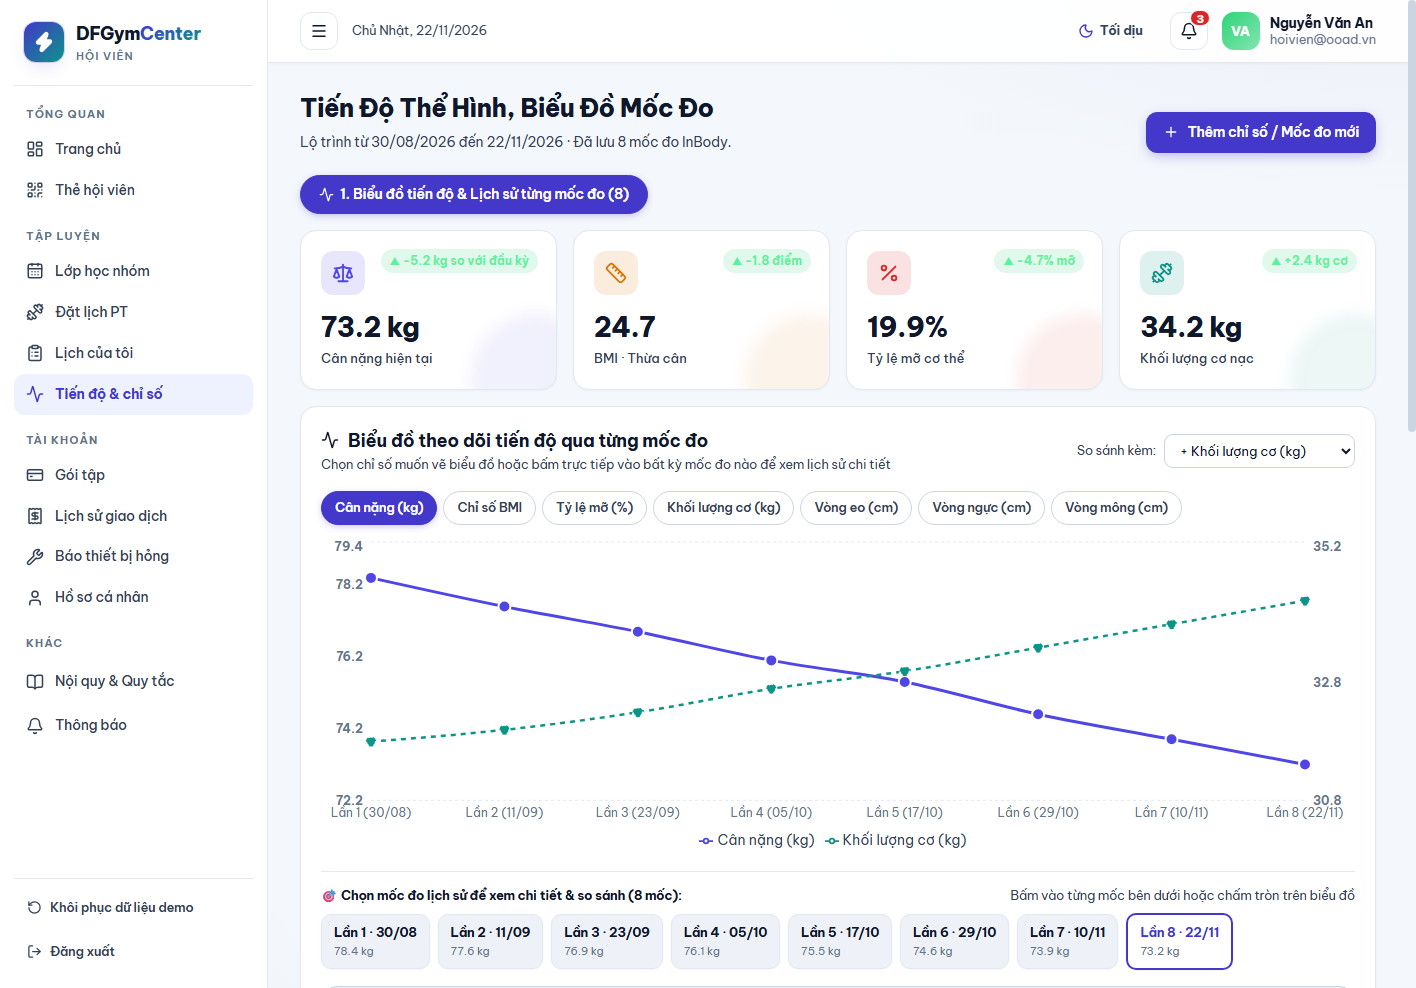
\includegraphics[width=0.92\textwidth]{images/ui_shunei/sh03_member_progress.png}
\caption{Giao diện màn hình Tiến độ thể hình \& Chỉ số cơ thể InBody (\texttt{/member/progress})}
\label{fig:sh-member-progress}
\end{figure}

\par\medskip\noindent\textbf{Danh sách các thành phần giao diện}\par\smallskip
{\footnotesize
\setlength{\tabcolsep}{2.5pt}
\begin{longtable}{|c|L{2.95cm}|L{1.85cm}|L{2.95cm}|L{2.75cm}|L{1.90cm}|L{2.05cm}|}
\hline
\textbf{STT} & \textbf{Tên} & \textbf{Kiểu} & \textbf{Ý nghĩa} & \textbf{Miền giá trị} & \textbf{Giá trị mặc định} & \textbf{Ghi chú} \\
\hline
\endfirsthead
\hline
\textbf{STT} & \textbf{Tên} & \textbf{Kiểu} & \textbf{Ý nghĩa} & \textbf{Miền giá trị} & \textbf{Giá trị mặc định} & \textbf{Ghi chú} \\
\hline
\endhead
\hline
\endfoot
\hline
\caption{Danh sách các thành phần giao diện -- Màn hình Tiến độ thể hình \& InBody} \\
\endlastfoot
1 & \texttt{Btn\_ThemMocDo} & Button & Mở hộp thoại nhập liệu một mốc đo InBody mới & Kích hoạt & \texttt{"+ Thêm chỉ số / Mốc đo mới"} & Tự động tính BMI khi nhập cân nặng, chiều cao \\ \hline
2 & \texttt{Card\_TongQuanBienThien} & Card Panel & Cụm 4 thẻ chỉ số tổng quan (Cân nặng, BMI, Tỷ lệ mỡ, Khối lượng cơ nạc) kèm mức biến thiên so với mốc đầu kỳ & Dữ liệu tổng hợp từ \texttt{Body\_Metrics} & Theo mốc đo mới nhất & Hiển thị huy hiệu tăng/giảm trực quan \\ \hline
3 & \texttt{Chart\_TienDo} & Chart & Biểu đồ đường hai trục Y so sánh chỉ số chính và chỉ số phụ theo thời gian & Dữ liệu từ \texttt{Body\_Metrics} & Cân nặng vs. Khối lượng cơ & Có chip chọn chỉ số và combobox so sánh \\* \hline
4 & \texttt{Lst\_MocLichSu} & List View & Thanh chọn nhanh các mốc đo lịch sử và khối phân tích đối chiếu từng mốc & Toàn bộ mốc đo của hội viên & Mốc mới nhất & So sánh với mốc trước và mốc ban đầu \\ \hline
\end{longtable}
}

\par\medskip\noindent\textbf{Danh sách các biến cố}\par\smallskip
{\footnotesize
\setlength{\tabcolsep}{4pt}
\begin{longtable}{|c|L{3.5cm}|L{7.8cm}|L{3.5cm}|}
\hline
\textbf{STT} & \textbf{Điều kiện kích hoạt} & \textbf{Xử lý} & \textbf{Ghi chú} \\
\hline
\endfirsthead
\hline
\textbf{STT} & \textbf{Điều kiện kích hoạt} & \textbf{Xử lý} & \textbf{Ghi chú} \\
\hline
\endhead
\hline
\endfoot
\hline
\caption{Danh sách các biến cố -- Màn hình Tiến độ thể hình \& InBody} \\
\endlastfoot
0 & Khởi động màn hình (\texttt{/member/progress}) & Gọi API \texttt{GET /api/body-measurements/me} tải lịch sử mốc đo InBody; tính độ lệch so với mốc đầu kỳ cho \texttt{Card\_TongQuanBienThien}, vẽ \texttt{Chart\_TienDo} và hiển thị danh sách mốc trên \texttt{Lst\_MocLichSu}. & Hiển thị mốc mới nhất ở khung phân tích. \\ \hline
1 & Nhấn nút \texttt{Btn\_ThemMocDo} (\textit{+ Thêm chỉ số / Mốc đo mới}) & Mở hộp thoại nhập chỉ số: ngày đo, cân nặng, chiều cao, \% mỡ, khối lượng cơ, số đo 3 vòng và ghi chú; tự động tính chỉ số BMI khi nhập đủ cân nặng và chiều cao. & Kiểm tra tính hợp lệ trước khi lưu. \\* \hline
2 & Nhấn nút \textit{Lưu chỉ số} trong hộp thoại nhập liệu & Gửi yêu cầu \texttt{POST /api/body-measurements} lưu bản ghi mới vào bảng \texttt{Body\_Metrics}, đóng hộp thoại, hiển thị Toast \textit{``Đã lưu mốc đo chỉ số cơ thể thành công''} và làm mới biểu đồ tiến độ. & Bảo toàn mốc ban đầu không bị ghi đè. \\ \hline
\end{longtable}
}

% -------------------------------------------------------------------------
% 6.5.4 TRANG CHỦ HUẤN LUYỆN VIÊN (/trainer)
% -------------------------------------------------------------------------
\subsubsection{Màn hình Trang chủ Huấn luyện viên (Huấn luyện viên)}
Màn hình \textbf{Trang chủ Huấn luyện viên} (đường dẫn \texttt{/trainer}) là bảng điều khiển tổng hợp dành cho \textbf{Huấn luyện viên (PT)}, hiển thị thẻ chào mừng kèm chuyên môn và lối tắt nhanh, 4 thẻ KPI công việc, danh sách lịch dạy sắp tới trong 3 ngày, các buổi quá giờ cần điểm danh và đánh giá mới nhất từ học viên.

\begin{figure}[H]
\centering
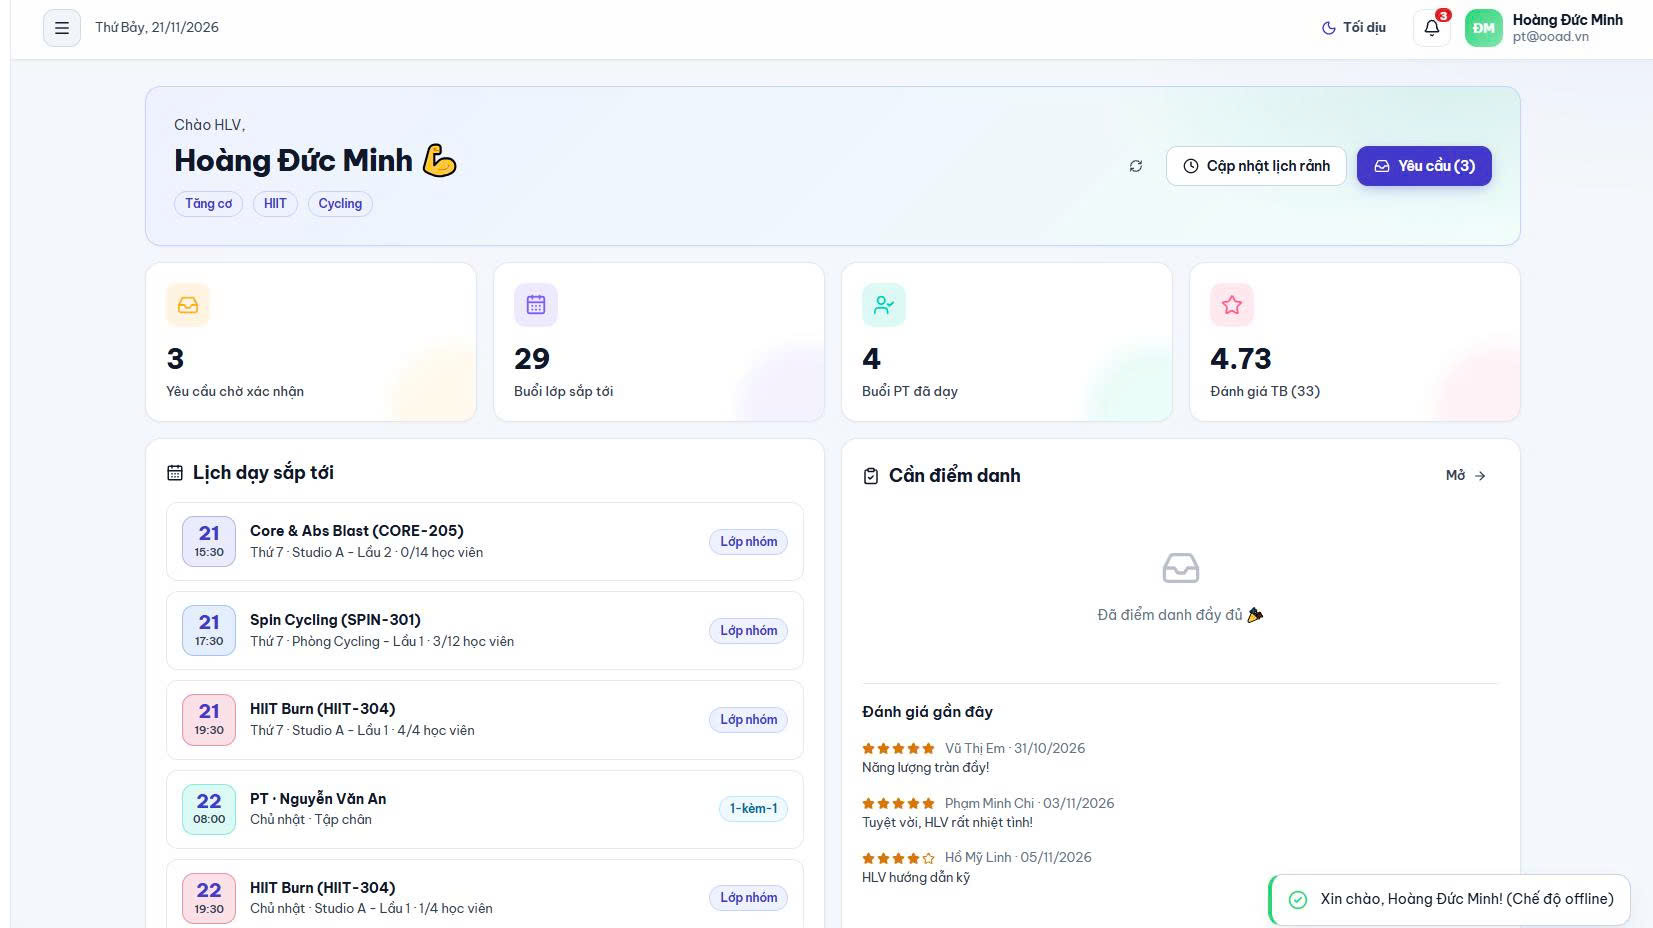
\includegraphics[width=0.92\textwidth]{images/ui_shunei/sh04_trainer_home.jpg}
\caption{Giao diện màn hình Trang chủ Huấn luyện viên (\texttt{/trainer})}
\label{fig:sh-trainer-home}
\end{figure}

\par\medskip\noindent\textbf{Danh sách các thành phần giao diện}\par\smallskip
{\footnotesize
\setlength{\tabcolsep}{2.5pt}
\begin{longtable}{|c|L{2.95cm}|L{1.85cm}|L{2.95cm}|L{2.75cm}|L{1.90cm}|L{2.05cm}|}
\hline
\textbf{STT} & \textbf{Tên} & \textbf{Kiểu} & \textbf{Ý nghĩa} & \textbf{Miền giá trị} & \textbf{Giá trị mặc định} & \textbf{Ghi chú} \\
\hline
\endfirsthead
\hline
\textbf{STT} & \textbf{Tên} & \textbf{Kiểu} & \textbf{Ý nghĩa} & \textbf{Miền giá trị} & \textbf{Giá trị mặc định} & \textbf{Ghi chú} \\
\hline
\endhead
\hline
\endfoot
\hline
\caption{Danh sách các thành phần giao diện -- Màn hình Trang chủ Huấn luyện viên} \\
\endlastfoot
1 & \texttt{Card\_HeroHLV} & Card Panel & Khối chào mừng hiển thị họ tên HLV và danh sách badge chuyên môn & Thông tin từ \texttt{Trainers} & Theo HLV đăng nhập & Nằm ở đầu trang \\ \hline
2 & \texttt{Btn\_\hspace{0pt}CapNhatRanh} & Button & Lối tắt mở màn hình thiết lập khung giờ rảnh (\texttt{/trainer/\hspace{0pt}availability}) & Kích hoạt & \texttt{"Cập nhật lịch rảnh"} & Hỗ trợ thao tác nhanh \\ \hline
3 & \texttt{Btn\_\hspace{0pt}YeuCauPT} & Button & Lối tắt mở danh sách yêu cầu PT (\texttt{/trainer/\hspace{0pt}requests}) kèm số lượng chờ & Kích hoạt & \texttt{"Yêu cầu (N)"} & \texttt{N} là số đơn đang \texttt{pending} \\ \hline
4 & \texttt{Stat\_ChoXacNhan} & StatCard & Thẻ KPI thống kê số yêu cầu đặt lịch PT 1-kèm-1 đang chờ duyệt & Số nguyên $\ge 0$ & $0$ & Tô màu vàng cảnh báo \\ \hline
5 & \texttt{Stat\_\hspace{0pt}LopSapToi} & StatCard & Thẻ KPI thống kê số buổi lớp nhóm sắp tới được phân công & Số nguyên $\ge 0$ & $0$ & Tổng hợp từ \texttt{Class\_\hspace{0pt}Sessions} \\ \hline
6 & \texttt{Stat\_PTDaDay} & StatCard & Thẻ KPI thống kê tổng số buổi PT 1-kèm-1 đã hoàn thành & Số nguyên $\ge 0$ & $0$ & Tính các buổi \texttt{completed} \\ \hline
7 & \texttt{Stat\_DanhGiaTB} & StatCard & Thẻ KPI hiển thị điểm sao trung bình và tổng số lượt đánh giá & Điểm $1.0$--$5.0$ (hoặc \texttt{--}) & Theo dữ liệu \texttt{Reviews} & Kèm tổng số đánh giá \\ \hline
8 & \texttt{Lst\_LichDaySapToi} & List View & Danh sách gộp lịch dạy lớp nhóm (2 ngày tới) và ca PT (3 ngày tới) & Tối đa $7$ buổi gần nhất & Sắp tăng dần theo giờ & Có badge phân biệt loại buổi \\ \hline
9 & \texttt{Lst\_CanDiemDanh} & List View & Danh sách tối đa 5 buổi lớp nhóm đã đến giờ nhưng chưa chốt điểm danh & Các buổi chưa điểm danh & Rỗng nếu đã điểm danh đủ & Gắn nhãn \textit{``Chưa điểm danh''} \\ \hline
10 & \texttt{Btn\_MoDiemDanh} & Button & Nút \textit{``Mở $\rightarrow$''} chuyển sang trang điểm danh lớp học (\texttt{/trainer/classes}) & Kích hoạt & \texttt{"Mở"} & Gắn ở góc khối Cần điểm danh \\* \hline
11 & \texttt{Lst\_DanhGiaGanDay} & List View & Hiển thị 3 nhận xét gần nhất kèm số sao và tên học viên & Bản ghi mới nhất từ \texttt{Reviews} & Tối đa $3$ mục & Giúp HLV nắm phản hồi nhanh \\ \hline
\end{longtable}
}

\par\medskip\noindent\textbf{Danh sách các biến cố}\par\smallskip
{\footnotesize
\setlength{\tabcolsep}{4pt}
\begin{longtable}{|c|L{3.5cm}|L{7.8cm}|L{3.5cm}|}
\hline
\textbf{STT} & \textbf{Điều kiện kích hoạt} & \textbf{Xử lý} & \textbf{Ghi chú} \\
\hline
\endfirsthead
\hline
\textbf{STT} & \textbf{Điều kiện kích hoạt} & \textbf{Xử lý} & \textbf{Ghi chú} \\
\hline
\endhead
\hline
\endfoot
\hline
\caption{Danh sách các biến cố -- Màn hình Trang chủ Huấn luyện viên} \\
\endlastfoot
0 & Khởi động màn hình (\texttt{/trainer}) & Gọi API \texttt{GET /api/trainers/me/pt-requests} lấy yêu cầu PT, \texttt{GET /api/reviews/me} lấy thống kê đánh giá và \texttt{GET /api/classes/sessions} tải lịch dạy; tính toán 4 chỉ số KPI, lịch sắp tới và danh sách cần điểm danh. & Cập nhật bộ đếm tức thời trên nút \texttt{Btn\_YeuCauPT}. \\ \hline
1 & Nhấn nút \texttt{Btn\_CapNhatRanh} hoặc \texttt{Btn\_YeuCauPT} & Điều hướng Huấn luyện viên sang màn hình quản lý khung giờ rảnh (\texttt{/trainer/availability}) hoặc hộp thư yêu cầu PT (\texttt{/trainer/requests}). & Chuyển màn hình làm việc nhanh. \\* \hline
2 & Nhấn nút \texttt{Btn\_MoDiemDanh} (\textit{Mở}) tại khối Cần điểm danh & Điều hướng sang màn hình \texttt{/trainer/classes} (tab \textit{Cần điểm danh}) để HLV mở hộp thoại điểm danh buổi học tương ứng. & Hỗ trợ nhắc việc không sót buổi. \\ \hline
\end{longtable}
}

% -------------------------------------------------------------------------
% 6.5.5 QUẢN LÝ YÊU CẦU & LỊCH HẸN PT (/trainer/requests)
% -------------------------------------------------------------------------
\subsubsection{Màn hình Quản lý Yêu cầu \& Lịch hẹn PT (Huấn luyện viên)}
Màn hình \textbf{Quản lý Yêu cầu \& Lịch hẹn PT} (đường dẫn \texttt{/trainer/requests}) cho phép \textbf{Huấn luyện viên} theo dõi các lịch hẹn 1-kèm-1 theo 3 tab trạng thái (\textit{Chờ xác nhận}, \textit{Đã xác nhận}, \textit{Lịch sử}), đồng thời thực hiện xác nhận, từ chối kèm lý do hoặc chốt hoàn thành/vắng mặt có đối chiếu trạng thái check-in tại quầy của hội viên.

\begin{figure}[H]
\centering
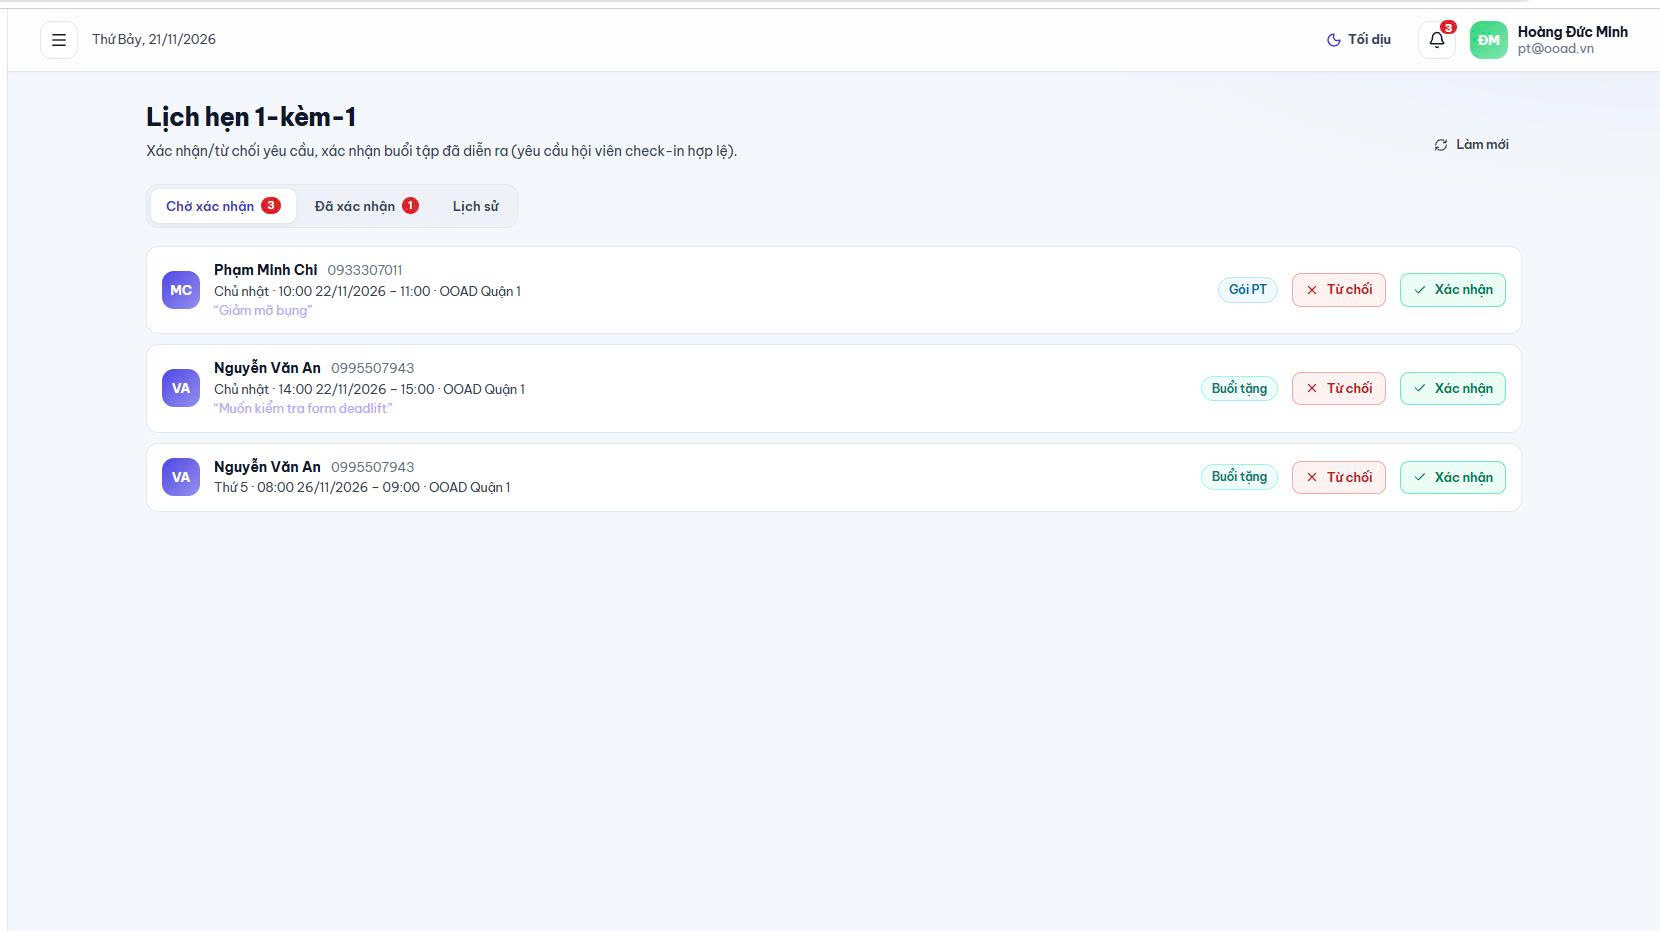
\includegraphics[width=0.92\textwidth]{images/ui_shunei/sh05_trainer_requests.jpg}
\caption{Giao diện màn hình Quản lý Yêu cầu \& Lịch hẹn PT (\texttt{/trainer/requests})}
\label{fig:sh-trainer-requests}
\end{figure}

\par\medskip\noindent\textbf{Danh sách các thành phần giao diện}\par\smallskip
{\footnotesize
\setlength{\tabcolsep}{2.5pt}
\begin{longtable}{|c|L{2.95cm}|L{1.85cm}|L{2.95cm}|L{2.75cm}|L{1.90cm}|L{2.05cm}|}
\hline
\textbf{STT} & \textbf{Tên} & \textbf{Kiểu} & \textbf{Ý nghĩa} & \textbf{Miền giá trị} & \textbf{Giá trị mặc định} & \textbf{Ghi chú} \\
\hline
\endfirsthead
\hline
\textbf{STT} & \textbf{Tên} & \textbf{Kiểu} & \textbf{Ý nghĩa} & \textbf{Miền giá trị} & \textbf{Giá trị mặc định} & \textbf{Ghi chú} \\
\hline
\endhead
\hline
\endfoot
\hline
\caption{Danh sách các thành phần giao diện -- Màn hình Quản lý Yêu cầu \& Lịch hẹn PT} \\
\endlastfoot
1 & \texttt{Tab\_TrangThaiPT} & Tab Group & Phân loại lịch hẹn PT theo 3 trạng thái xử lý & \{\texttt{"pending"}, \texttt{"confirmed"}, \texttt{"history"}\} & \texttt{"pending"} & Kèm bộ đếm số lượng từng tab \\ \hline
2 & \texttt{Btn\_XacNhanPT} & Button & Chấp nhận yêu cầu đặt lịch PT từ hội viên & Kích hoạt & \texttt{"Xác nhận"} & Chỉ hiển thị ở tab \textit{Chờ xác nhận} \\ \hline
3 & \texttt{Btn\_TuChoiPT} & Button & Từ chối yêu cầu đặt lịch kèm hộp thoại nhập lý do & Kích hoạt & \texttt{"Từ chối"} & Hoàn trả buổi tập và mở lại ca rảnh \\ \hline
4 & \texttt{Btn\_HoanThanhPT} & Button & Đánh dấu hoàn thành hoặc vắng mặt sau khi buổi tập diễn ra & Kích hoạt & \texttt{"Hoàn thành"} & Chỉ hiện khi đã tới giờ bắt đầu \\* \hline
5 & \texttt{Bdg\_CheckinHV} & Badge & Huy hiệu đối chiếu hội viên đã quét thẻ vào chi nhánh hay chưa & \{\texttt{"Đã check-in"}, \texttt{"Chưa check-in"}\} & Truy vấn từ \texttt{Checkins} & Điều kiện mở quyền đánh giá \\ \hline
\end{longtable}
}

\par\medskip\noindent\textbf{Danh sách các biến cố}\par\smallskip
{\footnotesize
\setlength{\tabcolsep}{4pt}
\begin{longtable}{|c|L{3.5cm}|L{7.8cm}|L{3.5cm}|}
\hline
\textbf{STT} & \textbf{Điều kiện kích hoạt} & \textbf{Xử lý} & \textbf{Ghi chú} \\
\hline
\endfirsthead
\hline
\textbf{STT} & \textbf{Điều kiện kích hoạt} & \textbf{Xử lý} & \textbf{Ghi chú} \\
\hline
\endhead
\hline
\endfoot
\hline
\caption{Danh sách các biến cố -- Màn hình Quản lý Yêu cầu \& Lịch hẹn PT} \\
\endlastfoot
0 & Khởi động màn hình (\texttt{/trainer/requests}) & Gọi API \texttt{GET /api/trainers/me/pt-requests} tải toàn bộ danh sách lịch hẹn 1-kèm-1 của HLV, phân nhóm vào 3 tab và hiển thị số lượng chờ duyệt trên tab \textit{Chờ xác nhận}. & Đối chiếu kèm dữ liệu check-in của học viên. \\ \hline
1 & Nhấn nút \texttt{Btn\_XacNhanPT} (\textit{Xác nhận}) & Gửi \texttt{POST /api/trainers/pt-requests/\{id\}/respond} với \texttt{Accept = true}; chuyển trạng thái lịch sang \texttt{CONFIRMED}, giữ khóa ca rảnh và gửi thông báo xác nhận tới hội viên. & Chuyển lịch sang tab \textit{Đã xác nhận}. \\ \hline
2 & Nhấn nút \texttt{Btn\_TuChoiPT} (\textit{Từ chối}) & Mở hộp thoại nhập lý do từ chối; khi xác nhận gửi \texttt{Accept = false}, hoàn lại 1 buổi PT cho hội viên, giải phóng ca rảnh và gửi thông báo kèm lý do cho hội viên. & Đảm bảo minh bạch lý do từ chối. \\* \hline
3 & Nhấn nút \texttt{Btn\_HoanThanhPT} (\textit{Hoàn thành}) & Gửi \texttt{POST /api/trainers/pt-requests/\{id\}/complete} với \texttt{Attended = true}; ghi nhận buổi tập thành công và mở quyền đánh giá cho hội viên. & Cập nhật số liệu trên Dashboard HLV. \\ \hline
\end{longtable}
}

% -------------------------------------------------------------------------
% 6.5.6 QUẢN LÝ KHUNG GIỜ RẢNH HLV (/trainer/availability)
% -------------------------------------------------------------------------
\subsubsection{Màn hình Quản lý Khung giờ rảnh Huấn luyện viên (Huấn luyện viên)}
Màn hình \textbf{Quản lý Khung giờ rảnh Huấn luyện viên} (đường dẫn \texttt{/trainer/availability}) giúp \textbf{Huấn luyện viên} mở các ca rảnh 1-kèm-1 với bộ kiểm tra trực tiếp 5 quy tắc vận hành (giờ mở cửa chi nhánh, đặt trước tối thiểu 2 giờ, giới hạn 8 ca/ngày, thời lượng chuẩn và chống trùng lịch lớp nhóm/ca PT) kèm lưới thời khóa biểu tuần trực quan.

\begin{figure}[H]
\centering
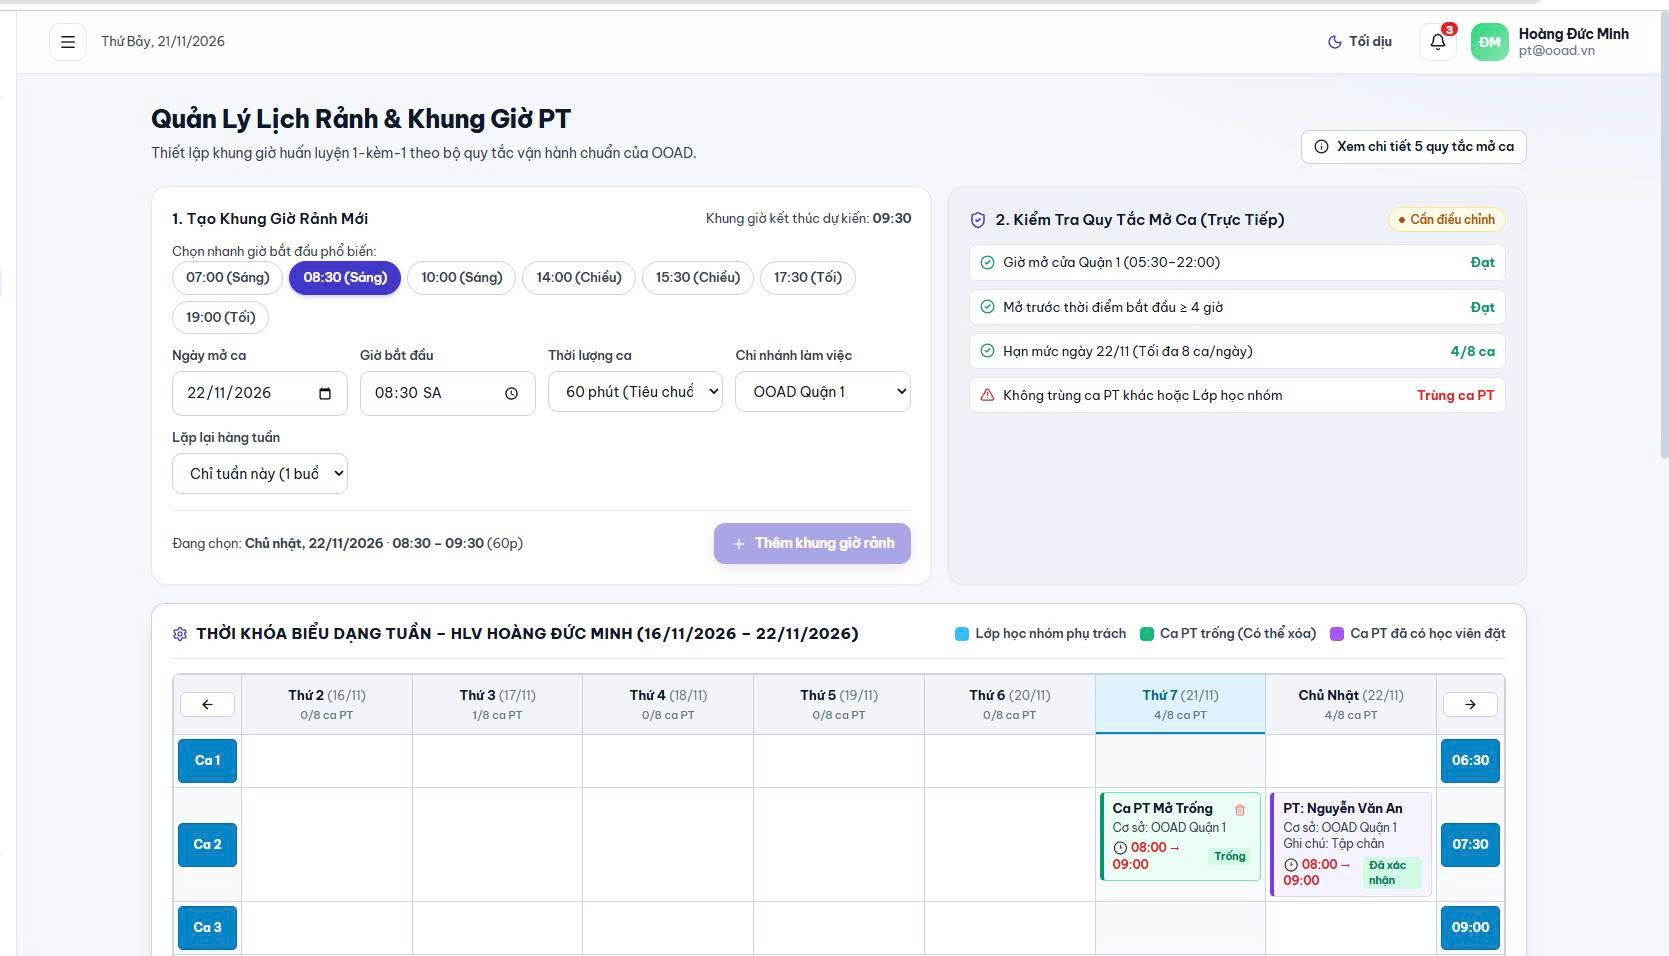
\includegraphics[width=0.92\textwidth]{images/ui_shunei/sh06_trainer_availability.jpg}
\caption{Giao diện màn hình Quản lý Khung giờ rảnh Huấn luyện viên (\texttt{/trainer/availability})}
\label{fig:sh-trainer-availability}
\end{figure}

\par\medskip\noindent\textbf{Danh sách các thành phần giao diện}\par\smallskip
{\footnotesize
\setlength{\tabcolsep}{2.5pt}
\begin{longtable}{|c|L{2.95cm}|L{1.85cm}|L{2.95cm}|L{2.75cm}|L{1.90cm}|L{2.05cm}|}
\hline
\textbf{STT} & \textbf{Tên} & \textbf{Kiểu} & \textbf{Ý nghĩa} & \textbf{Miền giá trị} & \textbf{Giá trị mặc định} & \textbf{Ghi chú} \\
\hline
\endfirsthead
\hline
\textbf{STT} & \textbf{Tên} & \textbf{Kiểu} & \textbf{Ý nghĩa} & \textbf{Miền giá trị} & \textbf{Giá trị mặc định} & \textbf{Ghi chú} \\
\hline
\endhead
\hline
\endfoot
\hline
\caption{Danh sách các thành phần giao diện -- Màn hình Quản lý Khung giờ rảnh HLV} \\
\endlastfoot
1 & \texttt{Btn\_\hspace{0pt}XemQuyTac} & Button & Mở hộp thoại mô tả chi tiết 5 quy tắc mở ca rảnh PT & Kích hoạt & \texttt{"Xem chi tiết 5 quy tắc mở ca"} & Mở \texttt{Dlg\_\hspace{0pt}QuyTacMoCa} \\ \hline
2 & \texttt{Chip\_GioNhanh} & Chip Button & Nhóm nút chọn nhanh giờ bắt đầu phổ biến (07:00 -- 19:00) & 7 mốc giờ (Sáng, Chiều, Tối) & \texttt{"08:30 (Sáng)"} & Tự điền vào ô \texttt{Txt\_GioBatDau} \\ \hline
3 & \texttt{Dt\_NgayMoCa} & DatePicker & Chọn ngày mở ca rảnh mới & Ngày $\ge$ ngày hiện tại & Ngày mai & Bắt buộc \\ \hline
4 & \texttt{Txt\_GioBatDau} & Textbox & Nhập hoặc chọn giờ bắt đầu ca tập & Định dạng \texttt{HH:mm} & \texttt{"08:30"} & Tự tính giờ kết thúc dự kiến \\ \hline
5 & \texttt{Cbo\_ThoiLuong} & ComboBox & Chọn thời lượng chuẩn cho ca dạy PT & \{\texttt{45p}, \texttt{60p}, \texttt{90p}\} & \texttt{60 phút (Tiêu chuẩn)} & Quy tắc thời lượng chuẩn \\ \hline
6 & \texttt{Cbo\_ChiNhanh} & ComboBox & Chọn chi nhánh nơi HLV nhận ca dạy & Các chi nhánh HLV trực thuộc & Chi nhánh đầu tiên & Lọc theo hồ sơ HLV \\ \hline
7 & \texttt{Cbo\_LapTuan} & ComboBox & Chọn số tuần lặp lại liên tiếp cho khung giờ mới & \{\texttt{1 tuần}, \texttt{2 tuần}, \texttt{4 tuần}\} & \texttt{Chỉ tuần này (1 buổi)} & Hỗ trợ mở lịch hàng loạt \\ \hline
8 & \texttt{Pnl\_KiemTraQuyTac} & Card Panel & Khối kiểm tra trực tiếp 5 quy tắc vận hành trước khi cho phép lưu ca & Trạng thái \textit{Đạt} / \textit{Vi phạm} & Đánh giá tự động theo form & Cảnh báo đỏ mục vi phạm \\ \hline
9 & \texttt{Btn\_\hspace{0pt}MoCaRanh} & Button & Lưu khung giờ rảnh mới lên hệ thống & Kích hoạt / Vô hiệu & \texttt{"+ Thêm khung giờ rảnh"} & Khóa khi \texttt{Pnl\_\hspace{0pt}KiemTraQuyTac} chưa đạt \\ \hline
10 & \texttt{Btn\_DieuHuongTuan} & Button Pair & Hai nút lùi (\texttt{$\leftarrow$}) và tiến (\texttt{$\rightarrow$}) tuần trên bảng thời khóa biểu & \texttt{weekIdx} $\in [-1, 2]$ & \texttt{weekIdx = 0} (tuần này) & Vô hiệu hóa ở hai biên \\ \hline
11 & \texttt{Tbl\_LichRanhTuan} & Matrix Table & Lưới thời khóa biểu $10$ ca $\times$ $7$ ngày hiển thị lớp nhóm, ca trống và ca đã đặt & Dữ liệu tuần của HLV & Tuần hiện tại & Nhấn tiêu đề ngày để chọn nhanh \texttt{Dt\_NgayMoCa} \\ \hline
12 & \texttt{Btn\_XoaCa} & Button & Xóa một ca rảnh còn trống chưa có hội viên đặt & Kích hoạt trên thẻ ca trống & Hiển thị trên từng ca trống & Ẩn với ca đã đặt hoặc đã qua \\* \hline
13 & \texttt{Dlg\_QuyTacMoCa} & Modal Dialog & Hộp thoại trình bày đầy đủ 5 quy tắc vận hành mở ca rảnh PT & Đóng / Mở & Đóng & Hiển thị khi nhấn \texttt{Btn\_XemQuyTac} \\ \hline
\end{longtable}
}

\par\medskip\noindent\textbf{Danh sách các biến cố}\par\smallskip
{\footnotesize
\setlength{\tabcolsep}{4pt}
\begin{longtable}{|c|L{3.5cm}|L{7.8cm}|L{3.5cm}|}
\hline
\textbf{STT} & \textbf{Điều kiện kích hoạt} & \textbf{Xử lý} & \textbf{Ghi chú} \\
\hline
\endfirsthead
\hline
\textbf{STT} & \textbf{Điều kiện kích hoạt} & \textbf{Xử lý} & \textbf{Ghi chú} \\
\hline
\endhead
\hline
\endfoot
\hline
\caption{Danh sách các biến cố -- Màn hình Quản lý Khung giờ rảnh HLV} \\
\endlastfoot
0 & Khởi động màn hình (\texttt{/trainer/\hspace{0pt}availability}) & Gọi API \texttt{GET /api/trainers/\{id\}/\hspace{0pt}availability} và tải danh sách buổi lớp nhóm được phân công; hiển thị lên lưới \texttt{Tbl\_LichRanhTuan} và chạy đánh giá trực tiếp trên \texttt{Pnl\_KiemTraQuyTac}. & Phân màu xanh dương (lớp), xanh lá (trống), tím (đã đặt). \\ \hline
1 & Thay đổi ngày, giờ, thời lượng, chi nhánh hoặc chọn \texttt{Chip\_GioNhanh} & Tự động tính giờ kết thúc và đối chiếu lại 5 quy tắc trên \texttt{Pnl\_KiemTraQuyTac} (giờ mở cửa, trước tối thiểu $2\text{h}$, tối đa 8 ca/ngày, thời lượng chuẩn 45/60/90 phút, không trùng ca PT/lớp nhóm) để bật hoặc khóa nút \texttt{Btn\_MoCaRanh}. & Phản hồi kiểm tra ngay khi người dùng đổi thông số. \\ \hline
2 & Nhấn nút \texttt{Btn\_MoCaRanh} (\textit{+ Thêm khung giờ rảnh}) & Gửi \texttt{POST /api/trainers/availability} (kèm số tuần lặp từ \texttt{Cbo\_LapTuan}); lưu các ca hợp lệ vào \texttt{Trainer\_Availabilities}, hiển thị Toast số ca thêm thành công và cập nhật lưới \texttt{Tbl\_LichRanhTuan}. & Báo lỗi nếu trùng lịch dạy lớp nhóm. \\* \hline
3 & Nhấn nút \texttt{Btn\_XoaCa} trên một thẻ ca PT trống & Kiểm tra ca chưa có học viên đặt và chưa đến giờ; gửi \texttt{DELETE /api/trainers/availability/\{id\}} để xóa khỏi CSDL và cập nhật lại lưới tuần. & Chặn xóa ca đã có hội viên đặt. \\ \hline
\end{longtable}
}

% -------------------------------------------------------------------------
% 6.5.7 ĐÁNH GIÁ TỪ HỘI VIÊN (/trainer/reviews)
% -------------------------------------------------------------------------
\subsubsection{Màn hình Đánh giá từ hội viên (Huấn luyện viên)}
Màn hình \textbf{Đánh giá từ hội viên} (đường dẫn \texttt{/trainer/reviews}) cho phép \textbf{Huấn luyện viên} theo dõi điểm đánh giá trung bình, biểu đồ phân phối $1$--$5$ sao cùng từng nhận xét chi tiết từ học viên sau các buổi PT và lớp nhóm. \textit{(Ghi chú: màn hình Hồ sơ chuyên môn Huấn luyện viên tại \texttt{/trainer/profile} đã được đặc tả đầy đủ tại mục~6.2.5.)}

\begin{figure}[H]
\centering
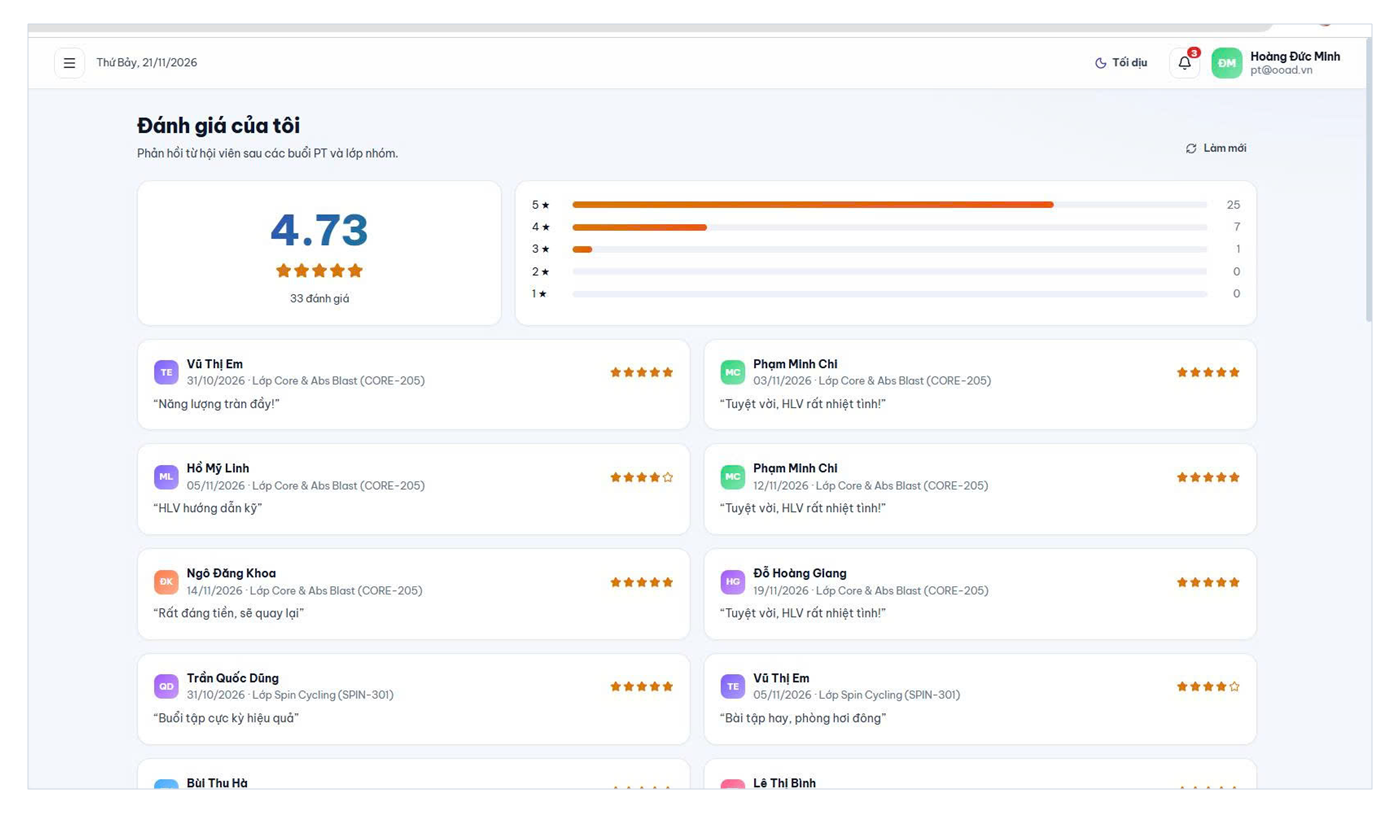
\includegraphics[width=0.92\textwidth]{images/ui_shunei/sh07_trainer_reviews_profile.png}
\caption{Giao diện màn hình Đánh giá từ hội viên (\texttt{/trainer/reviews})}
\label{fig:sh-trainer-reviews}
\end{figure}

\par\medskip\noindent\textbf{Danh sách các thành phần giao diện}\par\smallskip
{\footnotesize
\setlength{\tabcolsep}{2.5pt}
\begin{longtable}{|c|L{2.95cm}|L{1.85cm}|L{2.95cm}|L{2.75cm}|L{1.90cm}|L{2.05cm}|}
\hline
\textbf{STT} & \textbf{Tên} & \textbf{Kiểu} & \textbf{Ý nghĩa} & \textbf{Miền giá trị} & \textbf{Giá trị mặc định} & \textbf{Ghi chú} \\
\hline
\endfirsthead
\hline
\textbf{STT} & \textbf{Tên} & \textbf{Kiểu} & \textbf{Ý nghĩa} & \textbf{Miền giá trị} & \textbf{Giá trị mặc định} & \textbf{Ghi chú} \\
\hline
\endhead
\hline
\endfoot
\hline
\caption{Danh sách các thành phần giao diện -- Màn hình Đánh giá từ hội viên} \\
\endlastfoot
1 & \texttt{Lbl\_DiemTrungBinh} & Card Panel & Hiển thị điểm sao trung bình tổng hợp và tổng số lượt đánh giá & Điểm $1.0$--$5.0$ (hoặc \texttt{--}) & Tổng hợp từ \texttt{Reviews} & Làm tròn 2 chữ số thập phân \\ \hline
2 & \texttt{Prg\_PhanPhoiSao} & ProgressBar & 5 thanh tiến độ biểu diễn tỷ lệ phân phối đánh giá từ $5\bigstar$ đến $1\bigstar$ & $0\% \rightarrow 100\%$ & Tính theo từng mức sao & Kèm số lượng từng mức sao \\* \hline
3 & \texttt{Lst\_PhanHoiHV} & Card Grid & Danh sách thẻ phản hồi gồm tên hội viên, ngày gửi, tên lớp/buổi PT, sao và nhận xét & Danh sách từ \texttt{Reviews} & Toàn bộ đánh giá của HLV & Hiển thị Empty State nếu chưa có \\ \hline
\end{longtable}
}

\par\medskip\noindent\textbf{Danh sách các biến cố}\par\smallskip
{\footnotesize
\setlength{\tabcolsep}{4pt}
\begin{longtable}{|c|L{3.5cm}|L{7.8cm}|L{3.5cm}|}
\hline
\textbf{STT} & \textbf{Điều kiện kích hoạt} & \textbf{Xử lý} & \textbf{Ghi chú} \\
\hline
\endfirsthead
\hline
\textbf{STT} & \textbf{Điều kiện kích hoạt} & \textbf{Xử lý} & \textbf{Ghi chú} \\
\hline
\endhead
\hline
\endfoot
\hline
\caption{Danh sách các biến cố -- Màn hình Đánh giá từ hội viên} \\
\endlastfoot
0 & Khởi động màn hình (\texttt{/trainer/reviews}) & Gọi API \texttt{GET /api/reviews/me} tải điểm đánh giá trung bình lên \texttt{Lbl\_DiemTrungBinh}, tính tỷ lệ phân phối $1$--$5$ sao cho \texttt{Prg\_PhanPhoiSao} và kết xuất danh sách phản hồi lên \texttt{Lst\_PhanHoiHV}. & Tự động cập nhật khi có đánh giá mới. \\* \hline
1 & Nhấn nút \textit{Làm mới} ở góc trên bên phải & Gọi lại API \texttt{GET /api/reviews/me} để đồng bộ các nhận xét mới nhất vừa được hội viên gửi sau buổi tập. & Không làm gián đoạn phiên xem hiện tại. \\ \hline
\end{longtable}
}


\newpage
\subsection{Phân hệ Check-in / Check-out \& Thẻ hội viên}
Phân hệ \textbf{Check-in / Check-out \& Thẻ hội viên} bao gồm 7 màn hình phục vụ \textbf{Hội viên}, cổng tự động \textbf{Kiosk} và \textbf{Nhân viên Lễ tân / Quản trị viên} nhằm kiểm soát ra/vào chi nhánh theo thời gian thực, cấp/khóa/báo mất thẻ điện tử mã QR và tra cứu, kết xuất lịch sử check-in.

% =========================================================================
% 6.6.1 THẺ HỘI VIÊN & MÃ QR (/member/card)
% =========================================================================
\subsubsection{Màn hình Thẻ hội viên \& Mã QR (Hội viên)}
Màn hình \textbf{Thẻ hội viên \& Mã QR} (đường dẫn \texttt{/member/card}) cho phép \textbf{Hội viên} xuất trình thẻ điện tử kèm mã QR động để quét check-in/check-out, theo dõi trạng thái có mặt tại chi nhánh, xem lịch sử cấp thẻ và nhật ký ra/vào gần nhất, sao chép mã thẻ hoặc báo mất thẻ khẩn cấp.

\begin{figure}[H]
\centering
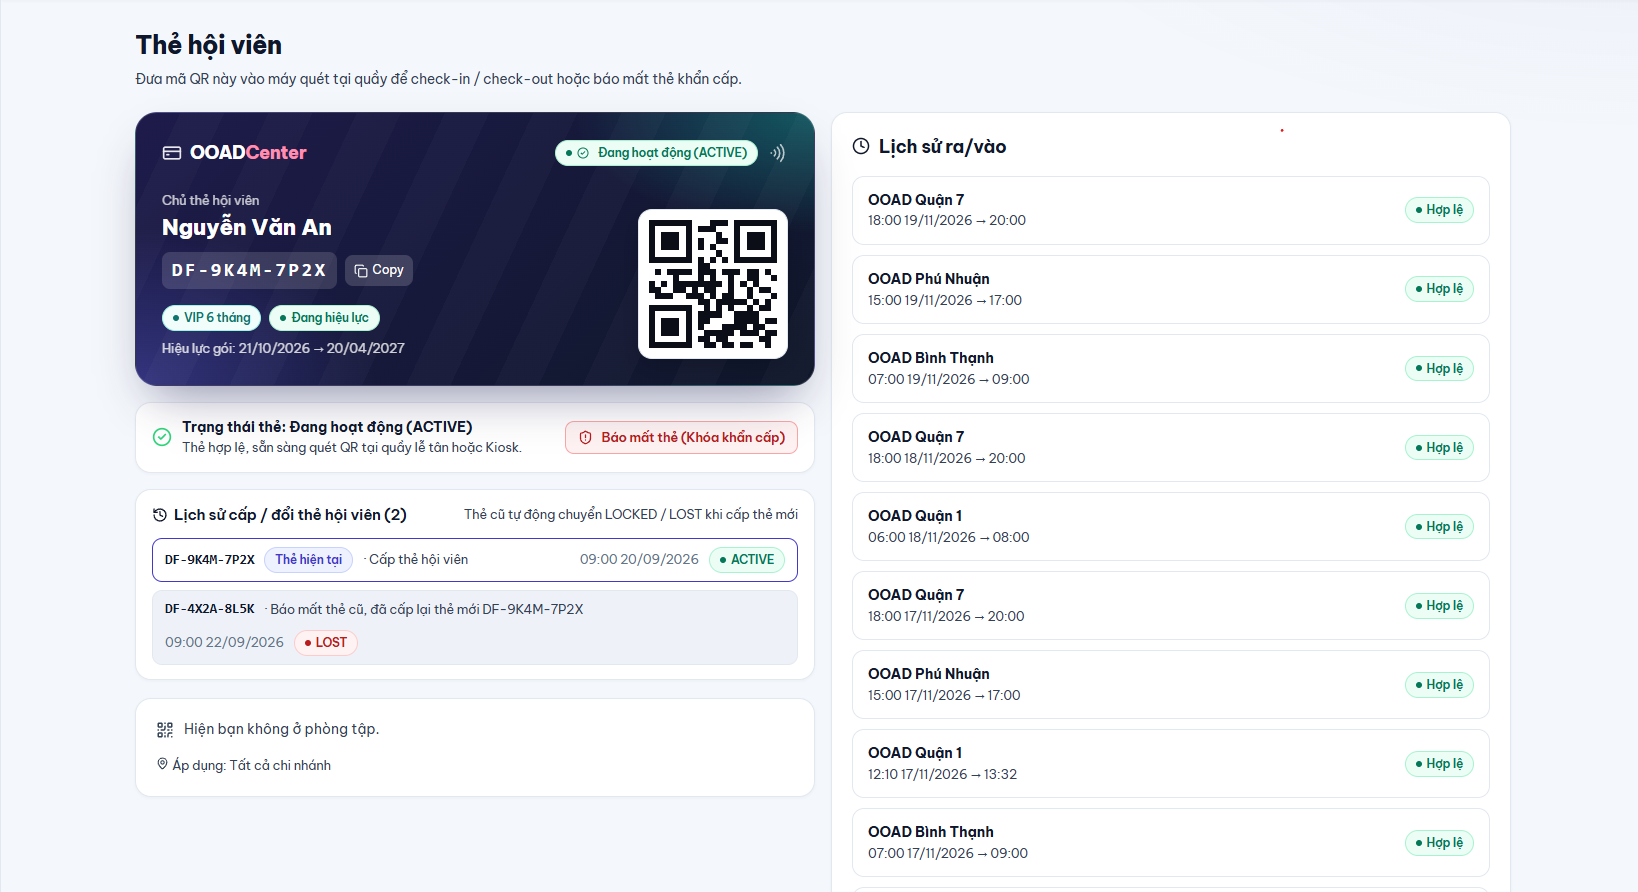
\includegraphics[width=0.92\textwidth]{images/ui_taok/mh01_member_card.png}
\caption{Giao diện màn hình Thẻ hội viên \& Mã QR (\texttt{/member/card})}
\label{fig:mh-member-card}
\end{figure}

\par\medskip\noindent\textbf{Danh sách các thành phần giao diện}\par\smallskip
{\footnotesize
\setlength{\tabcolsep}{2.5pt}
\begin{longtable}{|c|L{2.95cm}|L{1.85cm}|L{2.95cm}|L{2.75cm}|L{1.90cm}|L{2.05cm}|}
\hline
\textbf{STT} & \textbf{Tên} & \textbf{Kiểu} & \textbf{Ý nghĩa} & \textbf{Miền giá trị} & \textbf{Giá trị mặc định} & \textbf{Ghi chú} \\
\hline
\endfirsthead
\hline
\textbf{STT} & \textbf{Tên} & \textbf{Kiểu} & \textbf{Ý nghĩa} & \textbf{Miền giá trị} & \textbf{Giá trị mặc định} & \textbf{Ghi chú} \\
\hline
\endhead
\hline
\endfoot
\hline
\caption{Danh sách các thành phần giao diện -- Màn hình Thẻ hội viên \& Mã QR} \\
\endlastfoot
1 & \texttt{Lbl\_TieuDeThe} & Label & Tiêu đề màn hình \textit{``Thẻ hội viên''} & Chuỗi ký tự & \texttt{"Thẻ hội viên"} & Chỉ đọc \\ \hline
2 & \texttt{Pnl\_TheHoiVien} & Card Panel & Khối thẻ mô phỏng hiển thị chủ thẻ, gói tập và hạn sử dụng & Đối tượng thẻ & Theo user đăng nhập & Đổi màu đỏ (\texttt{LOST}) / vàng (\texttt{LOCKED}) \\ \hline
3 & \texttt{Img\_QRCode} & Image & Mã QR sinh tự động từ chuỗi \texttt{Card\_Code} & Chuỗi \texttt{Card\_Code} & Mã thẻ hiện tại & Kích thước $128\times128\text{px}$ \\ \hline
4 & \texttt{Lbl\_MaThe} & Label & Hiển thị mã thẻ định danh (ví dụ: \texttt{DF-1001}) & Chuỗi ký tự & \texttt{Card\_Code} & Phông monospace \\ \hline
5 & \texttt{Btn\_CopyMa} & Button & Sao chép nhanh chuỗi mã thẻ vào clipboard & Kích hoạt & \texttt{"Copy"} & Đổi thành \textit{``Đã chép''} trong $2\text{s}$ \\ \hline
6 & \texttt{Bdg\_TrangThaiThe} & Badge & Huy hiệu hiển thị trạng thái hiện tại của thẻ & \{\texttt{"ACTIVE"}, \texttt{"LOCKED"}, \texttt{"LOST"}\} & \texttt{"ACTIVE"} & Xanh / Vàng / Đỏ \\ \hline
7 & \texttt{Btn\_BaoMatThe} & Button & Mở hộp thoại xác nhận báo mất thẻ khẩn cấp & Kích hoạt / Ẩn & \texttt{"Báo mất thẻ"} & Ẩn khi thẻ đã ở trạng thái \texttt{LOST} \\ \hline
8 & \texttt{Dlg\_XacNhanMat} & Modal Dialog & Hộp thoại cảnh báo vô hiệu hóa vĩnh viễn và nhập lý do mất thẻ & Đóng / Mở & Đóng & Chứa ô \texttt{Txt\_LyDoMat} \\ \hline
9 & \texttt{Txt\_LyDoMat} & Textbox & Ô nhập lý do báo mất thẻ của hội viên & Chuỗi $\le 255$ ký tự & \texttt{"Làm rơi / thất lạc thẻ"} & Bắt buộc khi xác nhận báo mất \\* \hline
10 & \texttt{Lst\_LichSuRaVao} & List View & Danh sách tối đa 12 lượt check-in/out gần nhất và kết quả & Bản ghi từ \texttt{Checkins} & $12$ lượt gần nhất & Hiện lý do nếu bị từ chối \\ \hline
\end{longtable}
}

\par\medskip\noindent\textbf{Danh sách các biến cố}\par\smallskip
{\footnotesize
\setlength{\tabcolsep}{4pt}
\begin{longtable}{|c|L{3.5cm}|L{7.8cm}|L{3.5cm}|}
\hline
\textbf{STT} & \textbf{Điều kiện kích hoạt} & \textbf{Xử lý} & \textbf{Ghi chú} \\
\hline
\endfirsthead
\hline
\textbf{STT} & \textbf{Điều kiện kích hoạt} & \textbf{Xử lý} & \textbf{Ghi chú} \\
\hline
\endhead
\hline
\endfoot
\hline
\caption{Danh sách các biến cố -- Màn hình Thẻ hội viên \& Mã QR} \\
\endlastfoot
0 & Khởi động màn hình (\texttt{/member/card}) & Tải thông tin thẻ từ \texttt{Member\_Cards} (\texttt{Card\_Code}, \texttt{Status}), gói tập hiệu lực, lượt check-in đang mở (nếu có) và lịch sử ra/vào của hội viên; sinh mã QR từ \texttt{Card\_Code}. & Ẩn nút \texttt{Btn\_BaoMatThe} nếu thẻ đã \texttt{LOST}. \\ \hline
1 & Nhấn nút \texttt{Btn\_CopyMa} (\textit{Copy}) & Sao chép chuỗi \texttt{Card\_Code} vào clipboard và đổi nhãn nút sang \textit{``Đã chép''} trong $2$ giây. & Phản hồi tức thời. \\ \hline
2 & Nhấn nút \texttt{Btn\_BaoMatThe} (\textit{Báo mất thẻ}) & Mở hộp thoại \texttt{Dlg\_XacNhanMat}, hiển thị cảnh báo vô hiệu hóa vĩnh viễn và ô nhập lý do \texttt{Txt\_LyDoMat}. & Xác nhận trước thao tác không thể hoàn tác. \\ \hline
3 & Nhấn \textit{Xác nhận Báo mất} trong \texttt{Dlg\_XacNhanMat} & Kiểm tra quyền sở hữu thẻ; gọi \texttt{PATCH /api/member-cards/\{id\}/status} chuyển thẻ sang \texttt{LOST}, lưu lý do, đóng modal và thông báo thành công. & Thẻ chuyển màu đỏ; cổng quét QR sẽ từ chối mã này. \\* \hline
4 & Nhấn nút \textit{Hủy bỏ} trong hộp thoại & Đóng \texttt{Dlg\_XacNhanMat} và giữ nguyên trạng thái thẻ hiện tại. & Không phát sinh thay đổi dữ liệu. \\ \hline
\end{longtable}
}

% =========================================================================
% 6.6.2 KIOSK CHECK-IN / CHECK-OUT (/kiosk)
% =========================================================================
\subsubsection{Màn hình Kiosk Check-in / Check-out tự động (Khách / Cổng tự động)}
Màn hình \textbf{Kiosk Check-in / Check-out tự động} (đường dẫn \texttt{/kiosk}) vận hành tại cửa ra vào từng chi nhánh (không cần đăng nhập), cho phép chọn chi nhánh, quét mã thẻ/QR hoặc dùng nút quẹt nhanh để kiểm tra hiệu lực thẻ, gói tập, trạng thái Freeze, quyền tập chéo và tự động gắn cờ đã check-in (\texttt{CheckedIn}) cho các lịch lớp học/PT trong ngày làm cơ sở để HLV xác nhận điểm danh.

\begin{figure}[H]
\centering
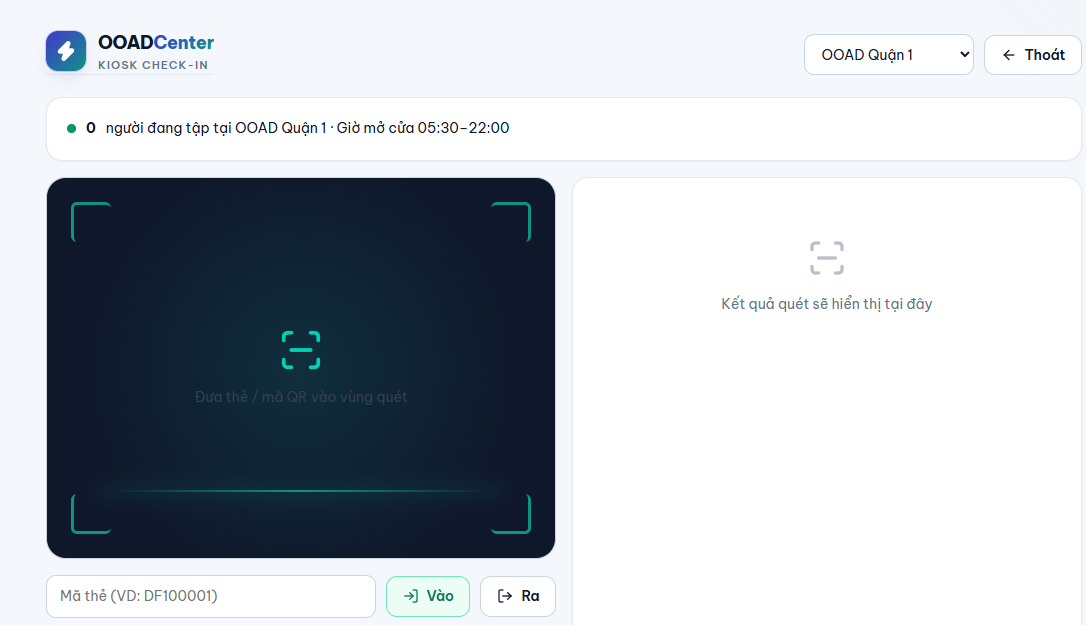
\includegraphics[width=0.92\textwidth]{images/ui_taok/mh02_kiosk.png}
\caption{Giao diện màn hình Kiosk Check-in / Check-out tự động (\texttt{/kiosk})}
\label{fig:mh-kiosk}
\end{figure}

\par\medskip\noindent\textbf{Danh sách các thành phần giao diện}\par\smallskip
{\footnotesize
\setlength{\tabcolsep}{2.5pt}
\begin{longtable}{|c|L{2.95cm}|L{1.85cm}|L{2.95cm}|L{2.75cm}|L{1.90cm}|L{2.05cm}|}
\hline
\textbf{STT} & \textbf{Tên} & \textbf{Kiểu} & \textbf{Ý nghĩa} & \textbf{Miền giá trị} & \textbf{Giá trị mặc định} & \textbf{Ghi chú} \\
\hline
\endfirsthead
\hline
\textbf{STT} & \textbf{Tên} & \textbf{Kiểu} & \textbf{Ý nghĩa} & \textbf{Miền giá trị} & \textbf{Giá trị mặc định} & \textbf{Ghi chú} \\
\hline
\endhead
\hline
\endfoot
\hline
\caption{Danh sách các thành phần giao diện -- Màn hình Kiosk Check-in / Check-out} \\
\endlastfoot
1 & \texttt{Cbo\_ChiNhanhKiosk} & ComboBox & Chọn chi nhánh đang đặt thiết bị Kiosk & Danh sách chi nhánh \texttt{ACTIVE} & Chi nhánh đầu tiên & Lọc số người đang tập theo chi nhánh \\ \hline
2 & \texttt{Lbl\_SoNguoiTap} & Label & Hiển thị số hội viên đang có mặt và giờ mở/đóng cửa & Số nguyên $\ge 0$ & Theo dữ liệu chi nhánh & Kèm chấm xanh trực tuyến \\ \hline
3 & \texttt{Pnl\_VungQuet} & Card Panel & Khung mô phỏng đầu đọc camera/QR kèm hiệu ứng quét & Trạng thái chờ quét & Luôn hiển thị & Hỗ trợ đầu đọc phần cứng \\ \hline
4 & \texttt{Txt\_MaTheKiosk} & Textbox & Ô nhập hoặc nhận chuỗi mã từ đầu đọc thẻ/QR & Chuỗi ký tự & Rỗng & Hỗ trợ nhấn phím \texttt{Enter} \\ \hline
5 & \texttt{Btn\_CheckIn} & Button & Thực hiện kiểm tra điều kiện và ghi nhận Check-in & Kích hoạt & \texttt{"Vào"} & Nút hành động màu xanh \\ \hline
6 & \texttt{Btn\_CheckOut} & Button & Thực hiện ghi nhận Check-out và tính thời lượng tập & Kích hoạt & \texttt{"Ra"} & Báo lỗi nếu chưa check-in \\ \hline
7 & \texttt{Chip\_QuetMoPhong} & Chip Button & Nhóm nút quẹt thẻ nhanh để kiểm thử nghiệp vụ Kiosk & Danh sách hội viên mẫu & $10$ hội viên đầu & Mô phỏng khi không có đầu đọc cứng \\ \hline
8 & \texttt{Pnl\_KetQua} & Card Panel & Khung kết quả hiển thị trạng thái Hợp lệ / Từ chối, tên gói và hạn dùng & Hợp lệ / Từ chối & Trạng thái chờ & Đổi viền xanh hoặc đỏ theo kết quả \\* \hline
9 & \texttt{Btn\_ThoatKiosk} & Button & Thoát chế độ Kiosk để quay về màn hình đăng nhập (\texttt{/login}) & Kích hoạt & \texttt{"Thoát"} & Đặt ở thanh tiêu đề trên \\ \hline
\end{longtable}
}

\par\medskip\noindent\textbf{Danh sách các biến cố}\par\smallskip
{\footnotesize
\setlength{\tabcolsep}{4pt}
\begin{longtable}{|c|L{3.5cm}|L{7.8cm}|L{3.5cm}|}
\hline
\textbf{STT} & \textbf{Điều kiện kích hoạt} & \textbf{Xử lý} & \textbf{Ghi chú} \\
\hline
\endfirsthead
\hline
\textbf{STT} & \textbf{Điều kiện kích hoạt} & \textbf{Xử lý} & \textbf{Ghi chú} \\
\hline
\endhead
\hline
\endfoot
\hline
\caption{Danh sách các biến cố -- Màn hình Kiosk Check-in / Check-out} \\
\endlastfoot
0 & Khởi động màn hình (\texttt{/kiosk}) & Tải danh sách chi nhánh đang hoạt động, mặc định chọn chi nhánh đầu tiên trên \texttt{Cbo\_ChiNhanhKiosk}; đếm số hội viên đang tập và hiển thị giờ đóng/mở cửa. & Không yêu cầu đăng nhập. \\ \hline
1 & Đổi lựa chọn trên \texttt{Cbo\_ChiNhanhKiosk} & Cập nhật \texttt{BranchId} hiện hành và tính lại số lượng hội viên đang có mặt tại chi nhánh mới chọn. & Xóa kết quả quét cũ trên \texttt{Pnl\_KetQua}. \\ \hline
2 & Nhập mã vào \texttt{Txt\_MaTheKiosk} và nhấn \texttt{Btn\_CheckIn} (hoặc \texttt{Enter}) & Kiểm tra thẻ \texttt{ACTIVE}, tài khoản không bị khóa, chưa có lượt check-in mở, gói còn hạn, không Freeze và đúng phạm vi chi nhánh; nếu hợp lệ tạo lượt check-in, tự động gắn cờ đã check-in (\texttt{CheckedIn}) cho lịch lớp/PT trong ngày để HLV đối chiếu điểm danh và hiển thị lên \texttt{Pnl\_KetQua}. & Xóa trắng ô nhập sau khi xử lý xong. \\ \hline
3 & Nhập mã vào \texttt{Txt\_MaTheKiosk} và nhấn \texttt{Btn\_CheckOut} & Tìm lượt check-in đang mở của hội viên, ghi nhận \texttt{Check\_Out\_At}, tính thời lượng buổi tập và hiển thị thông báo trên \texttt{Pnl\_KetQua}. & Báo lỗi nếu hội viên chưa check-in. \\ \hline
4 & Nhấn một nút trong nhóm \texttt{Chip\_QuetMoPhong} & Tự động nhận diện hội viên đang ở trong phòng hay ngoài phòng để gọi luồng Check-out hoặc Check-in tương ứng. & Hỗ trợ kiểm thử nhanh mọi kịch bản. \\* \hline
5 & Nhấn nút \texttt{Btn\_ThoatKiosk} (\textit{Thoát}) & Điều hướng trình duyệt trở về màn hình đăng nhập (\texttt{/login}). & Không thay đổi dữ liệu check-in. \\ \hline
\end{longtable}
}

% =========================================================================
% 6.6.3 TRANG CHỦ LỄ TÂN (/staff)
% =========================================================================
\subsubsection{Màn hình Trang chủ Lễ tân (Nhân viên Lễ tân)}
Màn hình \textbf{Trang chủ Lễ tân} (đường dẫn \texttt{/staff}) cung cấp cho \textbf{Nhân viên Lễ tân} bảng điều khiển vận hành theo ngày tại chi nhánh được phân công gồm 4 thẻ KPI (người đang có mặt, lượt check-in hôm nay, yêu cầu Freeze chờ duyệt, sự cố thiết bị đang mở), danh sách hội viên đang tập và lịch lớp học hôm nay.

\begin{figure}[H]
\centering
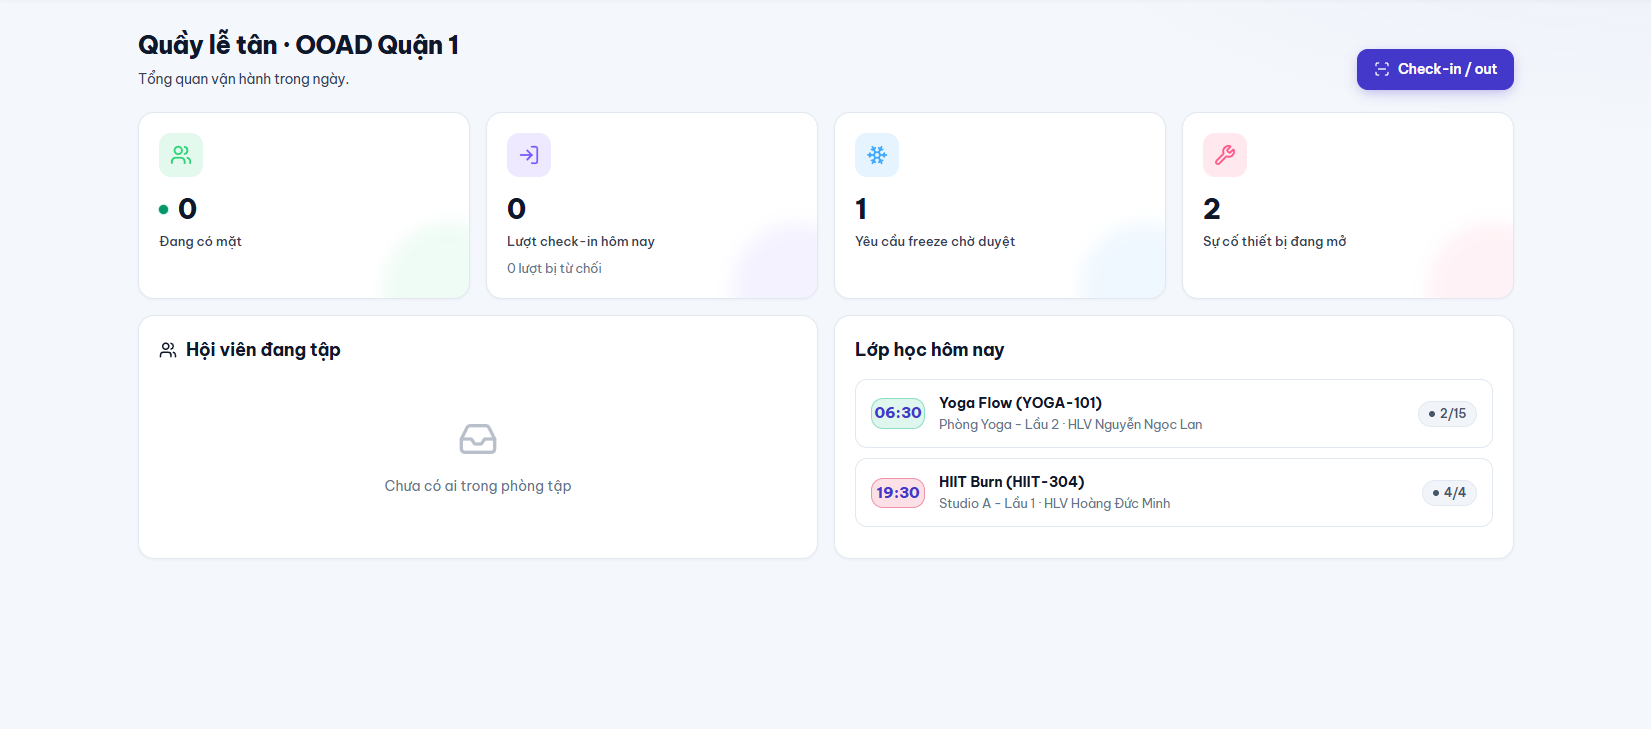
\includegraphics[width=0.92\textwidth]{images/ui_taok/mh03_staff_home.png}
\caption{Giao diện màn hình Trang chủ Lễ tân (\texttt{/staff})}
\label{fig:mh-staff-home}
\end{figure}

\par\medskip\noindent\textbf{Danh sách các thành phần giao diện}\par\smallskip
{\footnotesize
\setlength{\tabcolsep}{2.5pt}
\begin{longtable}{|c|L{2.95cm}|L{1.85cm}|L{2.95cm}|L{2.75cm}|L{1.90cm}|L{2.05cm}|}
\hline
\textbf{STT} & \textbf{Tên} & \textbf{Kiểu} & \textbf{Ý nghĩa} & \textbf{Miền giá trị} & \textbf{Giá trị mặc định} & \textbf{Ghi chú} \\
\hline
\endfirsthead
\hline
\textbf{STT} & \textbf{Tên} & \textbf{Kiểu} & \textbf{Ý nghĩa} & \textbf{Miền giá trị} & \textbf{Giá trị mặc định} & \textbf{Ghi chú} \\
\hline
\endhead
\hline
\endfoot
\hline
\caption{Danh sách các thành phần giao diện -- Màn hình Trang chủ Lễ tân} \\
\endlastfoot
1 & \texttt{Lbl\_TieuDeLeTan} & Label & Hiển thị tên quầy lễ tân kèm chi nhánh công tác & Chuỗi ký tự & Theo \texttt{BranchId} lễ tân & Chỉ đọc \\ \hline
2 & \texttt{Btn\_MoCheckin} & Button & Chuyển nhanh tới màn hình Quầy Check-in / Check-out & Kích hoạt & \texttt{"Check-in / out"} & Mở đường dẫn \texttt{/staff/\hspace{0pt}checkin} \\ \hline
3 & \texttt{Card\_DangCoMat} & StatCard & Đếm số hội viên đang tập tại chi nhánh (chưa check-out) & Số nguyên $\ge 0$ & $0$ & Có chấm xanh trực tuyến \\ \hline
4 & \texttt{Card\_LuotHomNay} & StatCard & Đếm tổng lượt check-in hợp lệ và từ chối trong ngày & Số nguyên $\ge 0$ & $0$ & Cập nhật theo thời gian thực \\ \hline
5 & \texttt{Card\_FreezeCho} & StatCard & Đếm số yêu cầu tạm ngưng gói tập đang chờ duyệt & Số nguyên $\ge 0$ & $0$ & Đồng bộ với trang \texttt{/staff/\hspace{0pt}freeze} \\ \hline
6 & \texttt{Card\_SuCoMo} & StatCard & Đếm số phản ánh sự cố thiết bị đang mở tại chi nhánh & Số nguyên $\ge 0$ & $0$ & Chỉ tính sự cố thuộc chi nhánh \\ \hline
7 & \texttt{Lst\_DangTap} & List View & Danh sách hội viên đang có mặt (\texttt{CheckOutAt == null}) & Danh sách \texttt{Checkins} & Rỗng nếu không có ai & Gắn nhãn \textit{Thủ công} nếu \texttt{Manual} \\* \hline
8 & \texttt{Lst\_LopHomNay} & List View & Danh sách buổi học nhóm diễn ra trong ngày tại chi nhánh & Danh sách \texttt{Class\_Sessions} & Rỗng nếu không có lớp & Hiện giờ, phòng, HLV và sĩ số \\ \hline
\end{longtable}
}

\par\medskip\noindent\textbf{Danh sách các biến cố}\par\smallskip
{\footnotesize
\setlength{\tabcolsep}{4pt}
\begin{longtable}{|c|L{3.5cm}|L{7.8cm}|L{3.5cm}|}
\hline
\textbf{STT} & \textbf{Điều kiện kích hoạt} & \textbf{Xử lý} & \textbf{Ghi chú} \\
\hline
\endfirsthead
\hline
\textbf{STT} & \textbf{Điều kiện kích hoạt} & \textbf{Xử lý} & \textbf{Ghi chú} \\
\hline
\endhead
\hline
\endfoot
\hline
\caption{Danh sách các biến cố -- Màn hình Trang chủ Lễ tân} \\
\endlastfoot
0 & Khởi động màn hình (\texttt{/staff}) & Gọi API \texttt{GET /api/staff/dashboard} theo \texttt{BranchId} của lễ tân; tổng hợp 4 chỉ số KPI, lọc danh sách lượt check-in đang mở lên \texttt{Lst\_DangTap} và lịch buổi học trong ngày lên \texttt{Lst\_LopHomNay}. & Chỉ hiển thị dữ liệu thuộc chi nhánh lễ tân trực. \\* \hline
1 & Nhấn nút \texttt{Btn\_MoCheckin} (\textit{Check-in / out}) & Điều hướng nhân viên lễ tân sang màn hình Quầy Check-in / Check-out (\texttt{/staff/checkin}). & Thao tác truy cập nhanh tại quầy. \\ \hline
\end{longtable}
}

% =========================================================================
% 6.6.4 QUẦY CHECK-IN / CHECK-OUT (/staff/checkin)
% =========================================================================
\subsubsection{Màn hình Quầy Check-in / Check-out (Nhân viên Lễ tân)}
Màn hình \textbf{Quầy Check-in / Check-out} (đường dẫn \texttt{/staff/checkin}) hỗ trợ \textbf{Nhân viên Lễ tân} thực hiện quét thẻ/QR tại quầy hoặc nhập check-in/check-out thủ công khi hội viên quên thẻ, thẻ hỏng hoặc lỗi máy quét, cho phép tìm kiếm hội viên, chọn lý do ngoại lệ và đối chiếu đầy đủ quy tắc gói tập.

\begin{figure}[H]
\centering
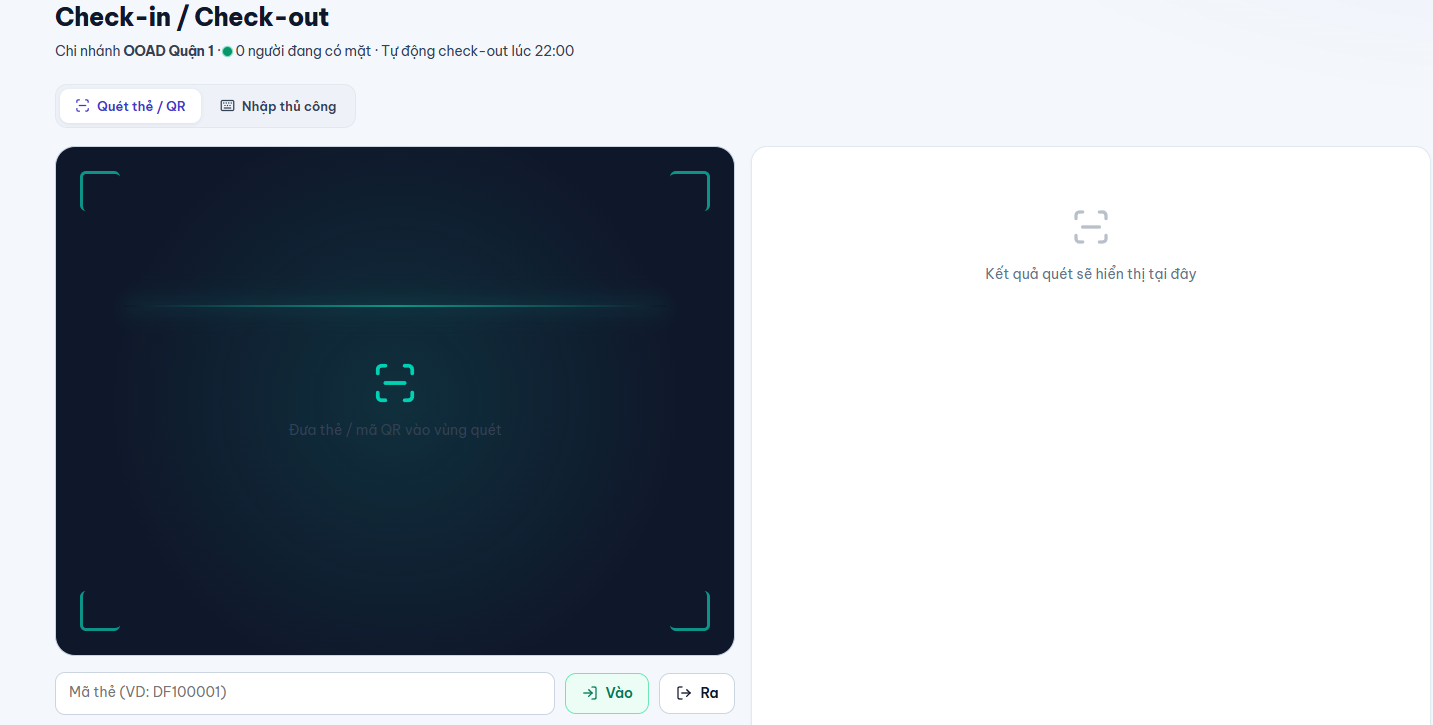
\includegraphics[width=0.92\textwidth]{images/ui_taok/mh04_staff_checkin.png}
\caption{Giao diện màn hình Quầy Check-in / Check-out tại Lễ tân (\texttt{/staff/checkin})}
\label{fig:mh-staff-checkin}
\end{figure}

\par\medskip\noindent\textbf{Danh sách các thành phần giao diện}\par\smallskip
{\footnotesize
\setlength{\tabcolsep}{2.5pt}
\begin{longtable}{|c|L{2.95cm}|L{1.85cm}|L{2.95cm}|L{2.75cm}|L{1.90cm}|L{2.05cm}|}
\hline
\textbf{STT} & \textbf{Tên} & \textbf{Kiểu} & \textbf{Ý nghĩa} & \textbf{Miền giá trị} & \textbf{Giá trị mặc định} & \textbf{Ghi chú} \\
\hline
\endfirsthead
\hline
\textbf{STT} & \textbf{Tên} & \textbf{Kiểu} & \textbf{Ý nghĩa} & \textbf{Miền giá trị} & \textbf{Giá trị mặc định} & \textbf{Ghi chú} \\
\hline
\endhead
\hline
\endfoot
\hline
\caption{Danh sách các thành phần giao diện -- Màn hình Quầy Check-in / Check-out} \\
\endlastfoot
1 & \texttt{Lbl\_ThongTinCa} & Label & Hiển thị chi nhánh trực, số người đang tập và giờ tự động check-out & Chuỗi ký tự & Theo chi nhánh lễ tân & Chỉ đọc \\ \hline
2 & \texttt{Tab\_CheDoQuay} & Tab Group & Chuyển đổi chế độ \textit{Quét thẻ / QR} và \textit{Nhập thủ công} & \{\texttt{"scan"}, \texttt{"manual"}\} & \texttt{"scan"} & Thao tác quầy linh hoạt \\ \hline
3 & \texttt{Txt\_TimHoiVien} & Textbox & Tìm kiếm hội viên theo họ tên, SĐT, email hoặc mã thẻ & Chuỗi $\ge 2$ ký tự & Rỗng & Hiển thị ở tab \textit{Nhập thủ công} \\ \hline
4 & \texttt{Chip\_LyDoThuCong} & Chip Button & Chọn lý do ngoại lệ khi lễ tân check-in thủ công & \{\texttt{"Quên thẻ"}, \texttt{"Thẻ bị hỏng"}, \texttt{"Máy quét lỗi"}, \texttt{"Khác"}\} & \texttt{"Quên thẻ"} & Lưu kèm vào nhật ký check-in \\ \hline
5 & \texttt{Lst\_KetQuaTim} & List View & Danh sách hội viên khớp từ khóa kèm ảnh đại diện, SĐT và mã thẻ & Tối đa $8$ hội viên & Rỗng & Giúp đối chiếu khuôn mặt tại quầy \\ \hline
6 & \texttt{Btn\_ThuCongInOut} & Button & Thực hiện Check-in hoặc Check-out thủ công cho dòng được chọn & \{\texttt{"Check-in"}, \texttt{"Check-out"}\} & Theo trạng thái mở & Hiển thị theo ngữ cảnh \\* \hline
7 & \texttt{Pnl\_KetQuaQuay} & Card Panel & Khung hiển thị kết quả kiểm tra gói tập, thông tin hội viên hoặc lý do từ chối & Hợp lệ / Từ chối & Trạng thái chờ & Dùng chung thành phần \texttt{ResultPanel} \\ \hline
\end{longtable}
}

\par\medskip\noindent\textbf{Danh sách các biến cố}\par\smallskip
{\footnotesize
\setlength{\tabcolsep}{4pt}
\begin{longtable}{|c|L{3.5cm}|L{7.8cm}|L{3.5cm}|}
\hline
\textbf{STT} & \textbf{Điều kiện kích hoạt} & \textbf{Xử lý} & \textbf{Ghi chú} \\
\hline
\endfirsthead
\hline
\textbf{STT} & \textbf{Điều kiện kích hoạt} & \textbf{Xử lý} & \textbf{Ghi chú} \\
\hline
\endhead
\hline
\endfoot
\hline
\caption{Danh sách các biến cố -- Màn hình Quầy Check-in / Check-out} \\
\endlastfoot
0 & Khởi động màn hình (\texttt{/staff/checkin}) & Gắn \texttt{BranchId} và \texttt{StaffId} của nhân viên lễ tân đang trực; mặc định mở tab \textit{Quét thẻ / QR} và hiển thị số người đang tập trên \texttt{Lbl\_ThongTinCa}. & Giờ đóng cửa tự động check-out lấy từ chi nhánh. \\ \hline
1 & Chuyển tab trên \texttt{Tab\_CheDoQuay} (\textit{Quét thẻ / QR} $\leftrightarrow$ \textit{Nhập thủ công}) & Chuyển vùng thao tác tương ứng giữa khung quét thẻ/QR và biểu mẫu tìm kiếm nhập tay ngoại lệ. & Đặt lại bộ lọc tìm kiếm khi chuyển tab. \\ \hline
2 & Nhập từ khóa ($\ge 2$ ký tự) vào \texttt{Txt\_TimHoiVien} & Lọc danh sách hội viên khớp tên, SĐT, email hoặc mã thẻ (tối đa $8$ kết quả) lên \texttt{Lst\_KetQuaTim}; kiểm tra trạng thái đang tập để hiển thị nút \textit{Check-in} hay \textit{Check-out}. & Nếu dưới $2$ ký tự thì giữ danh sách trống. \\ \hline
3 & Nhấn chọn một lý do trong \texttt{Chip\_LyDoThuCong} & Cập nhật biến \texttt{Reason} (\textit{Quên thẻ}, \textit{Thẻ bị hỏng}, \textit{Máy quét lỗi}, \textit{Khác}) và đánh dấu chip đang chọn. & Mặc định là \textit{``Quên thẻ''}. \\ \hline
4 & Nhấn nút \texttt{Btn\_ThuCongInOut} ở trạng thái \textit{Check-in} & Gửi \texttt{POST /api/checkins/manual} (\texttt{Method = Manual}, \texttt{CardId = NULL}, lưu \texttt{RecordedBy = StaffId} và \texttt{Reason}); kiểm tra đầy đủ điều kiện gói và hiển thị kết quả lên \texttt{Pnl\_KetQuaQuay}. & Lưu vết nhân viên thao tác thủ công. \\* \hline
5 & Nhấn nút \texttt{Btn\_ThuCongInOut} ở trạng thái \textit{Check-out} & Gửi yêu cầu check-out thủ công, ghi nhận \texttt{CheckOutAt}, tính thời lượng tập và cập nhật kết quả lên \texttt{Pnl\_KetQuaQuay}. & Cập nhật lại số người đang tập tại chi nhánh. \\ \hline
\end{longtable}
}

% =========================================================================
% 6.6.5 QUẢN LÝ CẤP / KHÓA / BÁO MẤT THẺ (/staff/member-cards)
% =========================================================================
\subsubsection{Màn hình Quản lý Cấp / Khóa / Báo mất thẻ (Nhân viên Lễ tân)}
Màn hình \textbf{Quản lý Cấp / Khóa / Báo mất thẻ} (đường dẫn \texttt{/staff/member-cards}) cho phép \textbf{Nhân viên Lễ tân} theo dõi thống kê toàn bộ thẻ hội viên (\texttt{ACTIVE}, \texttt{LOCKED}, \texttt{LOST}), lọc và tìm kiếm theo từ khóa, xem mã QR cùng lịch sử thẻ, thực hiện khóa/mở khóa/báo mất hoặc cấp thẻ mới (sinh mã ngẫu nhiên và chuyển thẻ cũ sang trạng thái \texttt{Replaced}).

\begin{figure}[H]
\centering
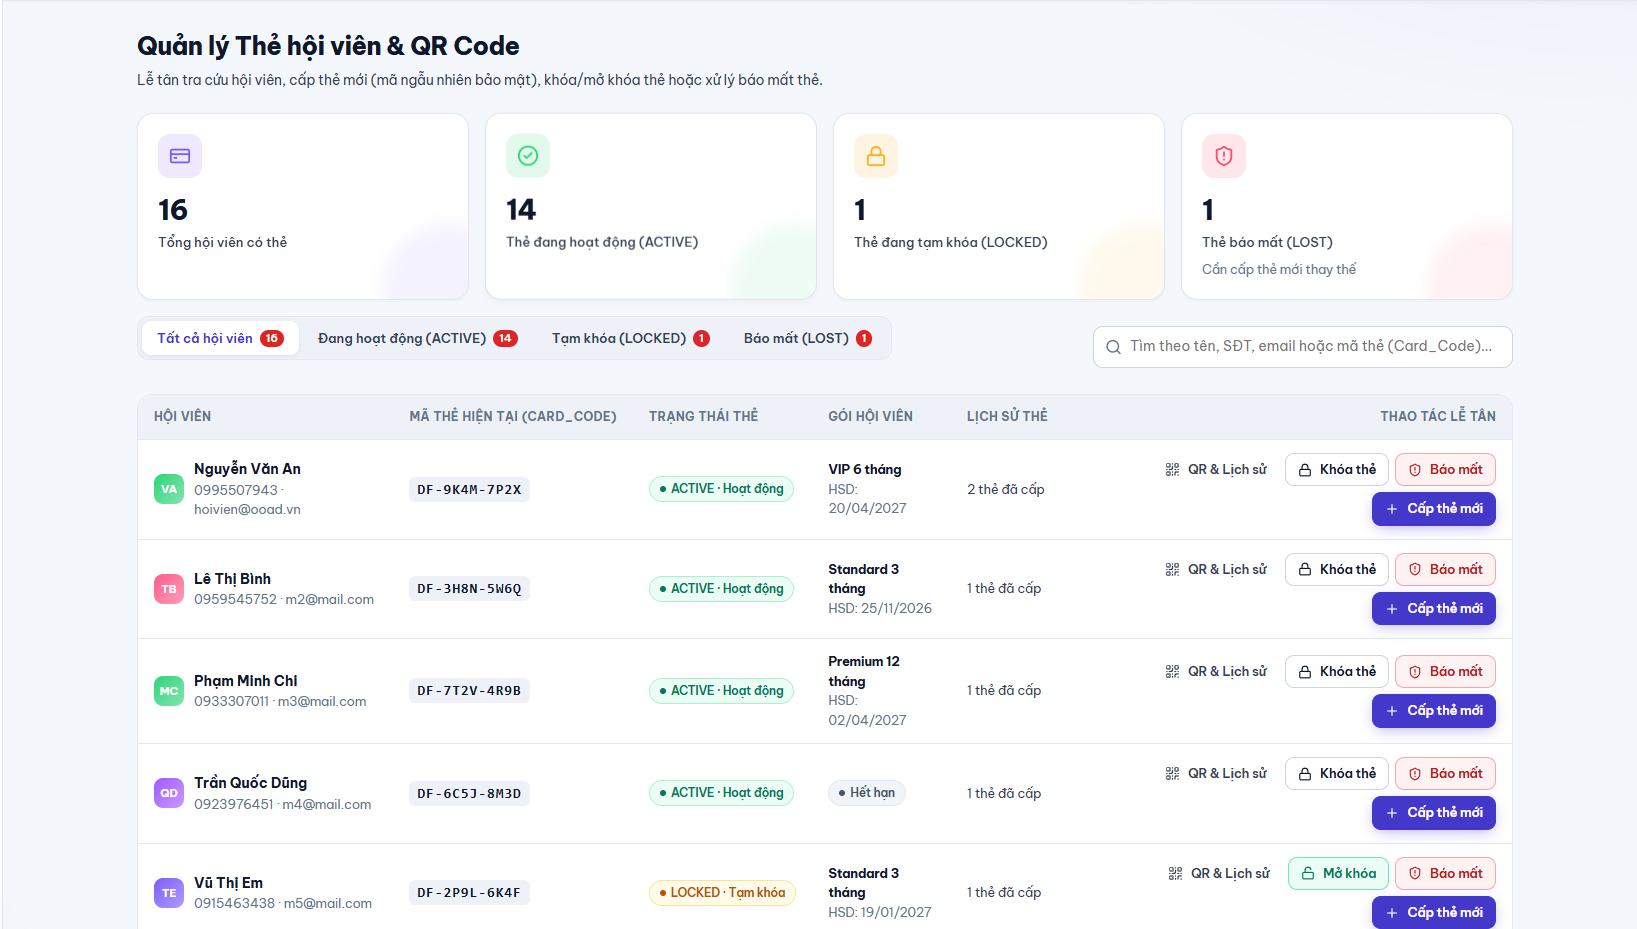
\includegraphics[width=0.92\textwidth]{images/ui_taok/mh05_member_cards.png}
\caption{Giao diện màn hình Quản lý Cấp / Khóa / Báo mất thẻ hội viên (\texttt{/staff/member-cards})}
\label{fig:mh-staff-cards}
\end{figure}

\par\medskip\noindent\textbf{Danh sách các thành phần giao diện}\par\smallskip
{\footnotesize
\setlength{\tabcolsep}{2.5pt}
\begin{longtable}{|c|L{2.95cm}|L{1.85cm}|L{2.95cm}|L{2.75cm}|L{1.90cm}|L{2.05cm}|}
\hline
\textbf{STT} & \textbf{Tên} & \textbf{Kiểu} & \textbf{Ý nghĩa} & \textbf{Miền giá trị} & \textbf{Giá trị mặc định} & \textbf{Ghi chú} \\
\hline
\endfirsthead
\hline
\textbf{STT} & \textbf{Tên} & \textbf{Kiểu} & \textbf{Ý nghĩa} & \textbf{Miền giá trị} & \textbf{Giá trị mặc định} & \textbf{Ghi chú} \\
\hline
\endhead
\hline
\endfoot
\hline
\caption{Danh sách các thành phần giao diện -- Màn hình Quản lý Thẻ hội viên} \\
\endlastfoot
1 & \texttt{Card\_ThongKeThe} & StatCard & Bộ 4 thẻ thống kê Tổng thẻ, \texttt{ACTIVE}, \texttt{LOCKED}, \texttt{LOST} & Số nguyên $\ge 0$ & Theo dữ liệu \texttt{Member\_Cards} & Tự cập nhật khi đổi trạng thái \\ \hline
2 & \texttt{Tab\_TrangThaiThe} & Tab Group & Lọc bảng danh sách theo trạng thái hiện tại của thẻ & \{\texttt{"ALL"}, \texttt{"ACTIVE"}, \texttt{"LOCKED"}, \texttt{"LOST"}\} & \texttt{"ALL"} & Kèm bộ đếm số lượng từng tab \\ \hline
3 & \texttt{Txt\_TimThe} & Textbox & Tìm nhanh theo tên, SĐT, email hoặc \texttt{Card\_Code} & Chuỗi ký tự & Rỗng & Lọc tức thời khi nhập \\ \hline
4 & \texttt{Grd\_DanhSachThe} & DataGrid & Bảng 6 cột (\textit{Hội viên}, \textit{Mã thẻ}, \textit{Trạng thái}, \textit{Gói hội viên}, \textit{Lịch sử thẻ}, \textit{Thao tác}) & Bản ghi từ \texttt{Member\_Cards} & Toàn bộ hội viên & Hiển thị màu badge theo trạng thái \\ \hline
5 & \texttt{Btn\_XemQR} & Button & Mở hộp thoại xem mã QR và lịch sử các thẻ đã cấp & Kích hoạt & \texttt{"QR \& Lịch sử"} & Gắn trên từng dòng bảng \\ \hline
6 & \texttt{Btn\_DoiTrangThai} & Button & Thực hiện Khóa (\texttt{LOCKED}), Mở khóa (\texttt{ACTIVE}) hoặc Báo mất (\texttt{LOST}) & Kích hoạt theo ngữ cảnh & Theo trạng thái thẻ & Thẻ \texttt{LOST} không cho mở khóa lại \\ \hline
7 & \texttt{Btn\_CapTheMoi} & Button & Mở hộp thoại \texttt{Dlg\_CapTheMoi} cấp lại thẻ mới cho hội viên & Kích hoạt & \texttt{"Cấp thẻ mới"} & Tự động vô hiệu hóa thẻ cũ \\* \hline
8 & \texttt{Dlg\_CapTheMoi} & Modal Dialog & Hộp thoại chọn lý do cấp lại (mất thẻ hoặc hỏng thẻ), chuyển thẻ cũ sang \texttt{Replaced} và sinh mã thẻ mới & Đóng / Mở & Đóng & Hiển thị mã QR mới sau khi cấp \\ \hline
\end{longtable}
}

\par\medskip\noindent\textbf{Danh sách các biến cố}\par\smallskip
{\footnotesize
\setlength{\tabcolsep}{4pt}
\begin{longtable}{|c|L{3.5cm}|L{7.8cm}|L{3.5cm}|}
\hline
\textbf{STT} & \textbf{Điều kiện kích hoạt} & \textbf{Xử lý} & \textbf{Ghi chú} \\
\hline
\endfirsthead
\hline
\textbf{STT} & \textbf{Điều kiện kích hoạt} & \textbf{Xử lý} & \textbf{Ghi chú} \\
\hline
\endhead
\hline
\endfoot
\hline
\caption{Danh sách các biến cố -- Màn hình Quản lý Thẻ hội viên} \\
\endlastfoot
0 & Khởi động màn hình (\texttt{/staff/member-cards}) & Tải danh sách hội viên và thẻ từ \texttt{Member\_Cards}; tính 4 chỉ số thống kê lên \texttt{Card\_ThongKeThe} và hiển thị toàn bộ bảng (\texttt{ALL}) lên \texttt{Grd\_DanhSachThe}. & Đồng bộ số lượng trên các tab lọc. \\ \hline
1 & Chọn tab trên \texttt{Tab\_TrangThaiThe} hoặc nhập vào \texttt{Txt\_TimThe} & Lọc lại các dòng trên \texttt{Grd\_DanhSachThe} theo trạng thái thẻ và từ khóa tìm kiếm (họ tên, SĐT, email hoặc \texttt{Card\_Code}). & Lọc trực tiếp không cần tải lại trang. \\ \hline
2 & Nhấn \texttt{Btn\_DoiTrangThai} (\textit{Khóa thẻ} / \textit{Mở khóa} / \textit{Báo mất}) & Gọi \texttt{PATCH /api/member-cards/\{id\}/status} cập nhật trạng thái sang \texttt{LOCKED}, \texttt{ACTIVE} hoặc \texttt{LOST}; làm mới bảng và hiển thị Toast thông báo. & Thẻ \texttt{LOST} bị khóa vĩnh viễn theo State Machine. \\ \hline
3 & Nhấn nút \texttt{Btn\_XemQR} (\textit{QR \& Lịch sử}) & Mở hộp thoại chi tiết hiển thị thành phần \texttt{MemberCardWidget} gồm mã QR Code và lịch sử các thẻ cũ của hội viên. & Tiện đối chiếu hoặc in thẻ tại quầy. \\ \hline
4 & Nhấn nút \texttt{Btn\_CapTheMoi} (\textit{Cấp thẻ mới}) & Mở hộp thoại \texttt{Dlg\_CapTheMoi} cho hội viên được chọn, cho phép chọn lý do cấp lại (\textit{Mất thẻ (\texttt{Lost})} hoặc \textit{Hỏng thẻ (\texttt{Damaged})}) và nhập ghi chú bổ sung. & Chuẩn bị thông số cấp thẻ mới. \\* \hline
5 & Nhấn \textit{Cấp thẻ mới (Sinh mã ngẫu nhiên)} trong \texttt{Dlg\_CapTheMoi} & Gửi \texttt{POST /api/member-cards/issue}: chuyển thẻ cũ đang hoạt động sang trạng thái kết thúc \texttt{Replaced} (vô hiệu hóa vĩnh viễn theo State Diagram \texttt{MemberCard}) kèm lý do cấp lại, sinh \texttt{Card\_Code} ngẫu nhiên duy nhất trạng thái \texttt{ACTIVE} và hiển thị mã QR mới vừa cấp. & Cấp mã thẻ hợp lệ ngay lập tức. \\ \hline
\end{longtable}
}

% =========================================================================
% 6.6.6 LỊCH SỬ CHECK-IN (/staff/history, /admin/checkins)
% =========================================================================
\subsubsection{Màn hình Lịch sử Check-in (Nhân viên Lễ tân / Quản trị viên)}
Màn hình \textbf{Lịch sử Check-in} (đường dẫn \texttt{/staff/\hspace{0pt}history} cho \textbf{Nhân viên Lễ tân} và \texttt{/admin/\hspace{0pt}checkins} cho \textbf{Quản trị viên}) hiển thị nhật ký các lượt check-in/out (bao gồm lượt hợp lệ, lượt từ chối kèm lý do, lượt nhập tay và tự động check-out cuối ngày), hỗ trợ lọc đa tiêu chí và xuất tệp \texttt{.csv}.

\begin{figure}[H]
\centering
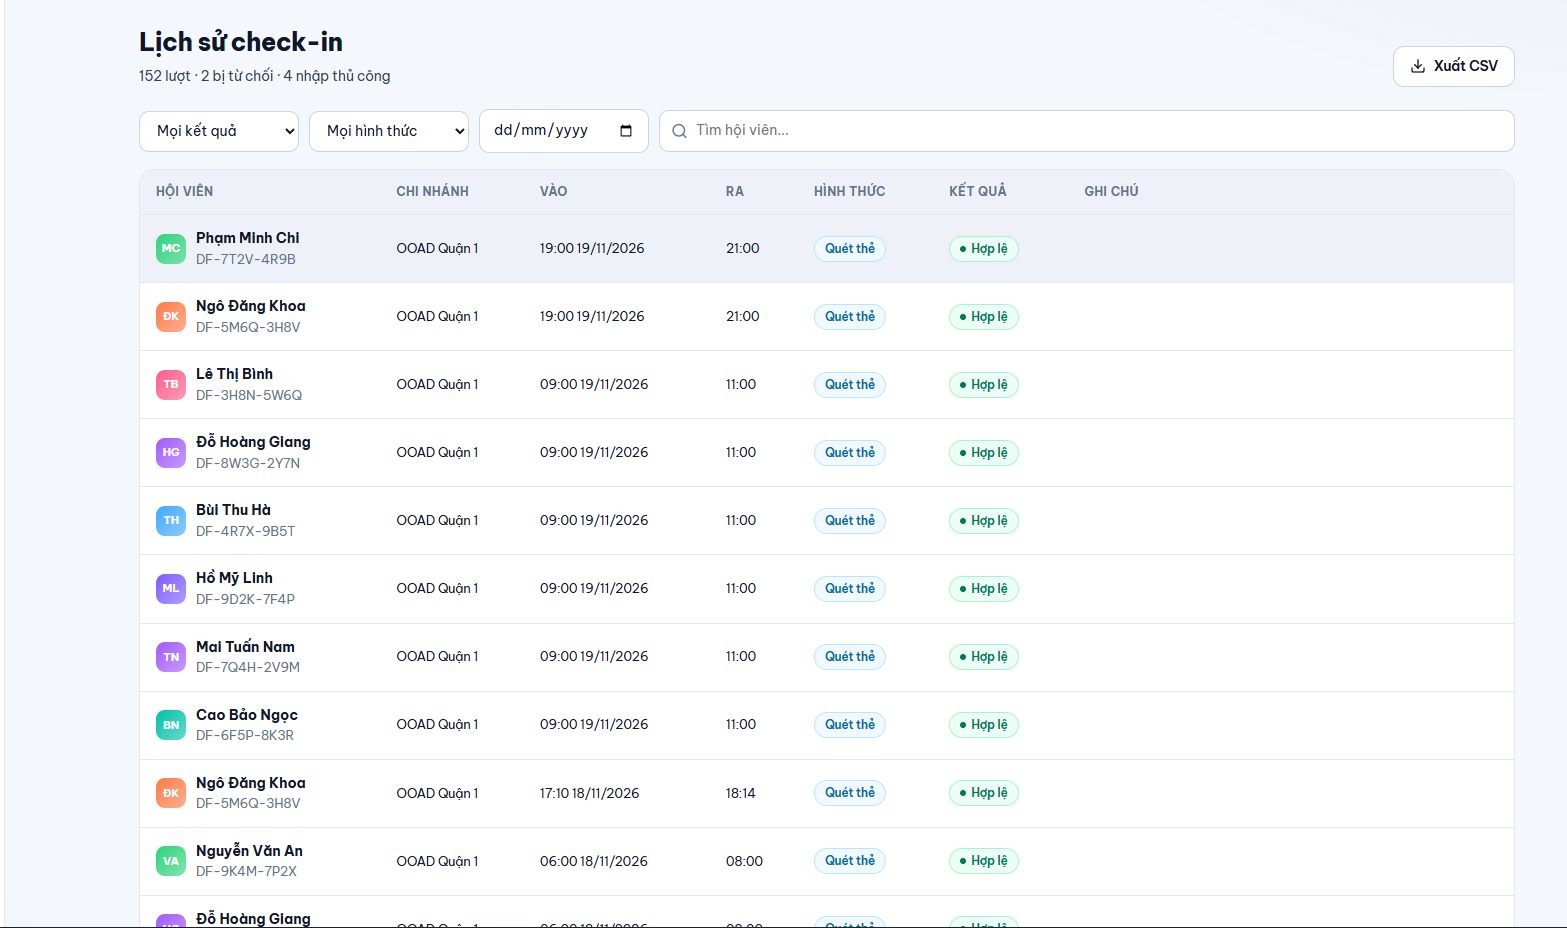
\includegraphics[width=0.92\textwidth]{images/ui_taok/mh06_checkin_history.png}
\caption{Giao diện màn hình Lịch sử Check-in / Check-out (\texttt{/staff/history})}
\label{fig:mh-checkin-history}
\end{figure}

\par\medskip\noindent\textbf{Danh sách các thành phần giao diện}\par\smallskip
{\footnotesize
\setlength{\tabcolsep}{2.5pt}
\begin{longtable}{|c|L{2.95cm}|L{1.85cm}|L{2.95cm}|L{2.75cm}|L{1.90cm}|L{2.05cm}|}
\hline
\textbf{STT} & \textbf{Tên} & \textbf{Kiểu} & \textbf{Ý nghĩa} & \textbf{Miền giá trị} & \textbf{Giá trị mặc định} & \textbf{Ghi chú} \\
\hline
\endfirsthead
\hline
\textbf{STT} & \textbf{Tên} & \textbf{Kiểu} & \textbf{Ý nghĩa} & \textbf{Miền giá trị} & \textbf{Giá trị mặc định} & \textbf{Ghi chú} \\
\hline
\endhead
\hline
\endfoot
\hline
\caption{Danh sách các thành phần giao diện -- Màn hình Lịch sử Check-in} \\
\endlastfoot
1 & \texttt{Lbl\_ThongKeNhanh} & Label & Tóm tắt tổng số lượt, lượt từ chối và lượt check-in thủ công & Chuỗi số liệu & Tính theo kết quả lọc & Tự cập nhật khi đổi bộ lọc \\ \hline
2 & \texttt{Btn\_XuatCSV} & Button & Kết xuất danh sách lượt check-in đang lọc ra tệp \texttt{.csv} & Kích hoạt & \texttt{"Xuất CSV"} & Mã hóa UTF-8 BOM chuẩn Excel \\ \hline
3 & \texttt{Cbo\_ChiNhanhLS} & ComboBox & Lọc lịch sử theo chi nhánh phòng tập & Tất cả / Danh sách chi nhánh & \texttt{"Tất cả chi nhánh"} & Chỉ hiển thị với Quản trị viên \\ \hline
4 & \texttt{Cbo\_KetQuaLS} & ComboBox & Lọc theo kết quả kiểm tra ra/vào & \{\texttt{"Mọi kết quả"}, \texttt{"Hợp lệ"}, \texttt{"Bị từ chối"}\} & \texttt{"Mọi kết quả"} & Kết hợp phép \texttt{AND} \\ \hline
5 & \texttt{Cbo\_HinhThucLS} & ComboBox & Lọc theo hình thức ghi nhận lượt check-in & \{\texttt{"Mọi hình thức"}, \texttt{"Quét thẻ"}, \texttt{"Thủ công"}\} & \texttt{"Mọi hình thức"} & Phân biệt Kiosk và quầy lễ tân \\ \hline
6 & \texttt{Dt\_NgayCheckin} & DatePicker & Lọc các lượt check-in trong một ngày cụ thể & Định dạng \texttt{yyyy-MM-dd} & Rỗng (mọi ngày) & Tùy chọn lọc ngày \\ \hline
7 & \texttt{Txt\_TimKiemLS} & Textbox & Tìm theo họ tên hoặc mã thẻ hội viên & Chuỗi ký tự & Rỗng & Lọc tức thời \\* \hline
8 & \texttt{Grd\_LichSuCheckin} & DataGrid & Bảng 7 cột (\textit{Hội viên}, \textit{Chi nhánh}, \textit{Vào}, \textit{Ra}, \textit{Hình thức}, \textit{Kết quả}, \textit{Ghi chú}) & Tối đa $200$ dòng mới nhất & Toàn bộ lượt khớp bộ lọc & Có badge phân biệt Hợp lệ / Từ chối \\ \hline
\end{longtable}
}

\par\medskip\noindent\textbf{Danh sách các biến cố}\par\smallskip
{\footnotesize
\setlength{\tabcolsep}{4pt}
\begin{longtable}{|c|L{3.5cm}|L{7.8cm}|L{3.5cm}|}
\hline
\textbf{STT} & \textbf{Điều kiện kích hoạt} & \textbf{Xử lý} & \textbf{Ghi chú} \\
\hline
\endfirsthead
\hline
\textbf{STT} & \textbf{Điều kiện kích hoạt} & \textbf{Xử lý} & \textbf{Ghi chú} \\
\hline
\endhead
\hline
\endfoot
\hline
\caption{Danh sách các biến cố -- Màn hình Lịch sử Check-in} \\
\endlastfoot
0 & Khởi động màn hình (\texttt{/staff/history} hoặc \texttt{/admin/checkins}) & Nếu là Lễ tân thì cố định lọc theo \texttt{BranchId} công tác (ẩn \texttt{Cbo\_ChiNhanhLS}); nếu là Admin thì mặc định chọn \textit{``Tất cả chi nhánh''}; tải tối đa 200 lượt mới nhất từ \texttt{Checkins}. & Hiển thị kèm nhân viên xử lý nếu nhập tay. \\ \hline
1 & Thay đổi bất kỳ bộ lọc nào trên thanh lọc & Kết hợp đồng thời điều kiện chi nhánh, kết quả, hình thức, ngày và từ khóa tìm kiếm theo phép toán \texttt{AND}; cập nhật \texttt{Grd\_LichSuCheckin} và \texttt{Lbl\_ThongKeNhanh}. & Phản hồi tức thời khi thay đổi điều kiện. \\* \hline
2 & Nhấn nút \texttt{Btn\_XuatCSV} (\textit{Xuất CSV}) & Gom toàn bộ danh sách đang hiển thị sau lọc, mã hóa UTF-8 BOM để hiển thị đúng tiếng Việt và tải xuống tệp \texttt{lich-su-checkin.csv}. & Phục vụ lưu trữ và báo cáo vận hành. \\ \hline
\end{longtable}
}

% =========================================================================
% 6.6.7 TRA CỨU HỘI VIÊN (/staff/members)
% =========================================================================
\subsubsection{Màn hình Tra cứu hội viên (Nhân viên Lễ tân)}
Màn hình \textbf{Tra cứu hội viên} (đường dẫn \texttt{/staff/members}) giúp \textbf{Nhân viên Lễ tân} tìm kiếm nhanh hồ sơ hội viên theo tên, SĐT, email hoặc mã thẻ để đối chiếu tình trạng tài khoản, mã thẻ, gói tập hiện tại, thời hạn hiệu lực và số buổi PT còn lại, đồng thời liên kết nhanh sang trang quản lý thẻ.

\begin{figure}[H]
\centering
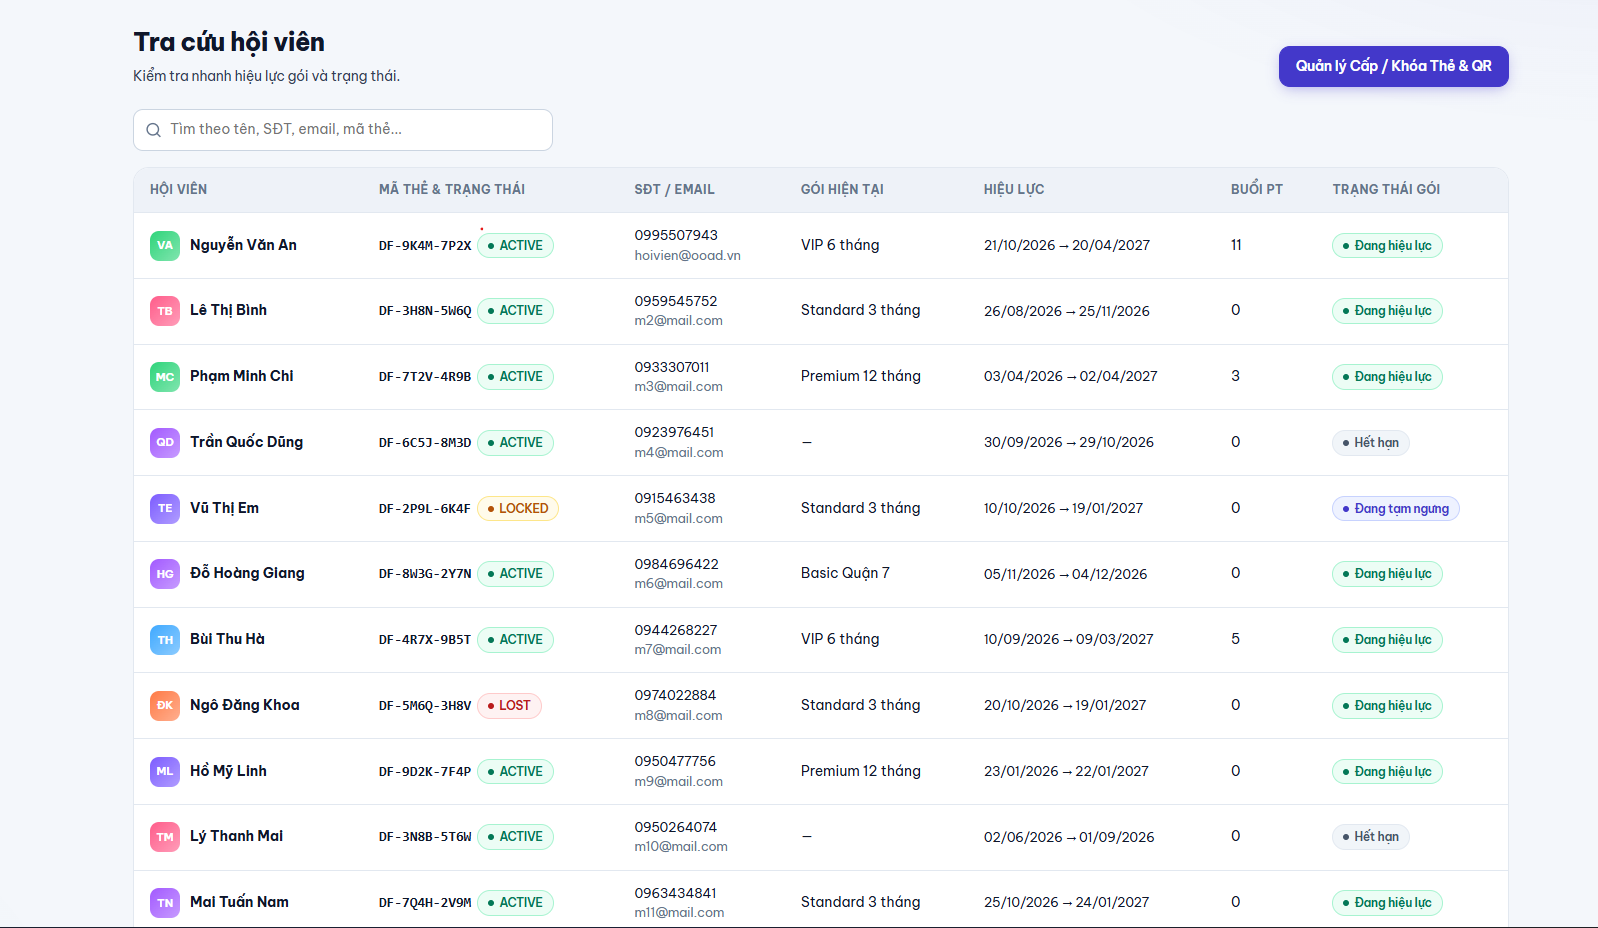
\includegraphics[width=0.92\textwidth]{images/ui_taok/mh07_staff_members.png}
\caption{Giao diện màn hình Tra cứu hội viên tại quầy Lễ tân (\texttt{/staff/members})}
\label{fig:mh-staff-members}
\end{figure}

\par\medskip\noindent\textbf{Danh sách các thành phần giao diện}\par\smallskip
{\footnotesize
\setlength{\tabcolsep}{2.5pt}
\begin{longtable}{|c|L{2.95cm}|L{1.85cm}|L{2.95cm}|L{2.75cm}|L{1.90cm}|L{2.05cm}|}
\hline
\textbf{STT} & \textbf{Tên} & \textbf{Kiểu} & \textbf{Ý nghĩa} & \textbf{Miền giá trị} & \textbf{Giá trị mặc định} & \textbf{Ghi chú} \\
\hline
\endfirsthead
\hline
\textbf{STT} & \textbf{Tên} & \textbf{Kiểu} & \textbf{Ý nghĩa} & \textbf{Miền giá trị} & \textbf{Giá trị mặc định} & \textbf{Ghi chú} \\
\hline
\endhead
\hline
\endfoot
\hline
\caption{Danh sách các thành phần giao diện -- Màn hình Tra cứu hội viên} \\
\endlastfoot
1 & \texttt{Btn\_QuanLyThe} & Button & Chuyển nhanh sang màn hình quản lý cấp, khóa và xem QR thẻ (\texttt{/staff/\hspace{0pt}member-cards}) & Kích hoạt & \texttt{"Quản lý Cấp / Khóa Thẻ \& QR"} & Gắn ở góc phải tiêu đề trang \\ \hline
2 & \texttt{Txt\_TimHoiVienTC} & Textbox & Nhập từ khóa tên, SĐT, email hoặc mã thẻ để lọc hội viên & Chuỗi ký tự & Rỗng & Lọc tức thời danh sách bảng \\* \hline
3 & \texttt{Grd\_HoiVien} & DataGrid & Bảng 7 cột (\textit{Hội viên}, \textit{Mã thẻ \& Trạng thái}, \textit{SĐT / Email}, \textit{Gói hiện tại}, \textit{Hiệu lực}, \textit{Buổi PT}, \textit{Trạng thái gói}) & Danh sách từ \texttt{Members} & Toàn bộ hội viên & Hiện trạng thái khóa nếu bị khóa \\ \hline
\end{longtable}
}

\par\medskip\noindent\textbf{Danh sách các biến cố}\par\smallskip
{\footnotesize
\setlength{\tabcolsep}{4pt}
\begin{longtable}{|c|L{3.5cm}|L{7.8cm}|L{3.5cm}|}
\hline
\textbf{STT} & \textbf{Điều kiện kích hoạt} & \textbf{Xử lý} & \textbf{Ghi chú} \\
\hline
\endfirsthead
\hline
\textbf{STT} & \textbf{Điều kiện kích hoạt} & \textbf{Xử lý} & \textbf{Ghi chú} \\
\hline
\endhead
\hline
\endfoot
\hline
\caption{Danh sách các biến cố -- Màn hình Tra cứu hội viên} \\
\endlastfoot
0 & Khởi động màn hình (\texttt{/staff/members}) & Gọi API \texttt{GET /api/members} tải danh sách toàn bộ hội viên kèm thông tin thẻ hiện tại, gói tập gần nhất, số buổi PT còn lại và trạng thái tài khoản lên \texttt{Grd\_HoiVien}. & Sẵn sàng đối chiếu khi khách tới quầy. \\ \hline
1 & Nhập từ khóa vào \texttt{Txt\_TimHoiVienTC} & Lọc tức thời các dòng có họ tên, email, SĐT hoặc mã thẻ chứa từ khóa vừa nhập và cập nhật lại bảng \texttt{Grd\_HoiVien}. & Không phân biệt chữ hoa/thường. \\* \hline
2 & Nhấn nút \texttt{Btn\_QuanLyThe} (\textit{Quản lý Cấp / Khóa Thẻ \& QR}) & Điều hướng nhân viên lễ tân sang màn hình quản lý thẻ hội viên (\texttt{/staff/member-cards}). & Hỗ trợ cấp lại thẻ ngay sau khi tra cứu. \\ \hline
\end{longtable}
}


\newpage
\subsection{Phân hệ Quản lý Thiết bị, Sự cố \& Báo cáo Thống kê}
Phân hệ \textbf{Quản lý Thiết bị, Sự cố \& Báo cáo Thống kê} phục vụ \textbf{Nhân viên Lễ tân} và \textbf{Quản trị viên} trong công tác theo dõi vòng đời máy tập, tiếp nhận xử lý phản ánh hỏng hóc và tổng hợp báo cáo tài chính, hội viên, hiệu suất vận hành đa chiều toàn hệ thống.

% ==========================================
% 6.7.1 QUẢN LÝ THIẾT BỊ & XỬ LÝ SỰ CỐ
% ==========================================
\subsubsection{Màn hình Quản lý Thiết bị và Sự cố (Nhân viên Lễ tân / Quản trị viên)}
Màn hình \textbf{Quản lý Thiết bị và Sự cố} (đường dẫn \texttt{/staff/equipment} cho \textbf{Nhân viên Lễ tân} giới hạn theo chi nhánh trực và \texttt{/admin/equipment} cho \textbf{Quản trị viên} toàn chuỗi) cho phép theo dõi tình trạng máy tập, bổ sung thiết bị mới và tiếp nhận, cập nhật tiến độ xử lý các phản ánh sự cố phát sinh.

\begin{figure}[H]
\centering
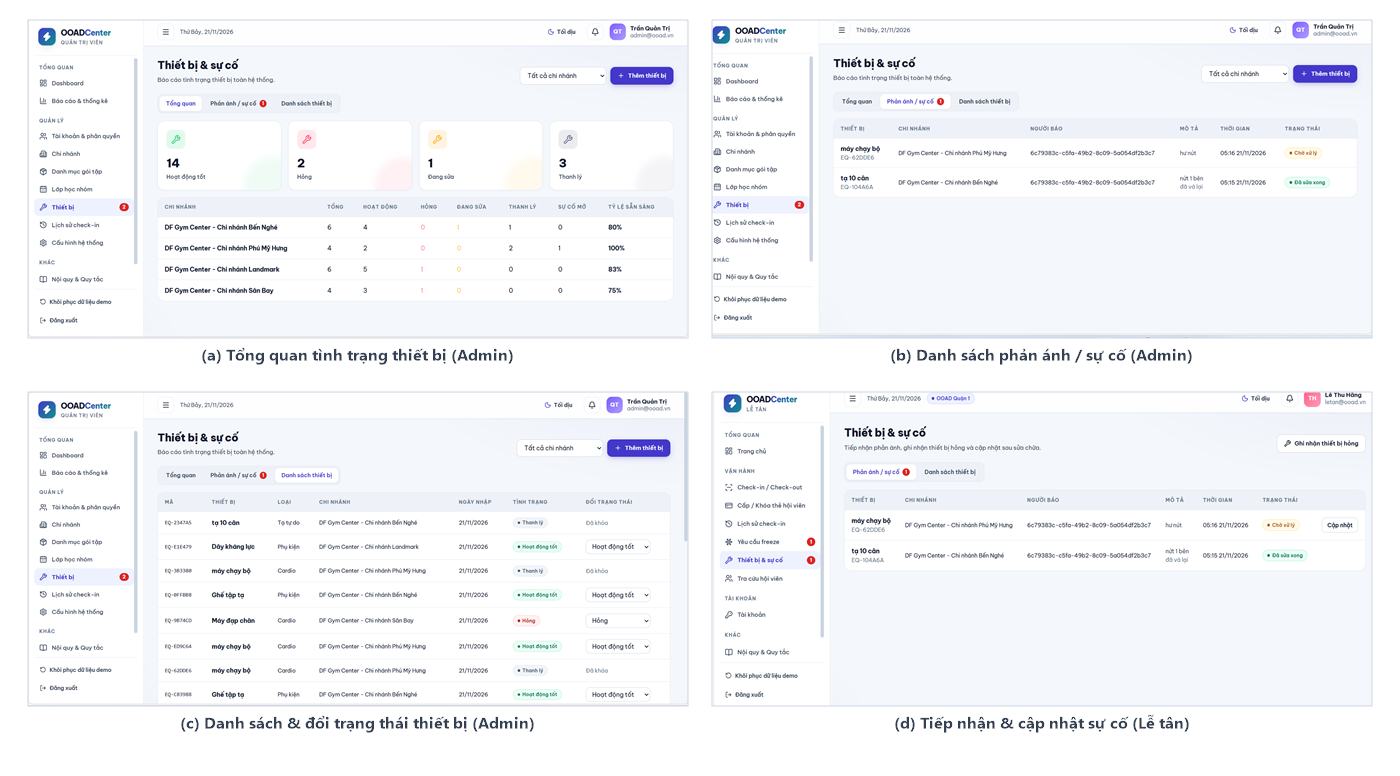
\includegraphics[width=0.92\textwidth]{images/ui_truc/mh09_equipment_manage.png}
\caption{Giao diện màn hình Quản lý Thiết bị và Sự cố}
\label{fig:mh09_equipment_manage}
\end{figure}

\par\medskip\noindent\textbf{Danh sách các thành phần giao diện}\par\smallskip
{\footnotesize
\setlength{\tabcolsep}{2.5pt}
\begin{longtable}{|c|L{2.95cm}|L{1.85cm}|L{2.95cm}|L{2.75cm}|L{1.90cm}|L{2.05cm}|}
\hline
\textbf{STT} & \textbf{Tên} & \textbf{Kiểu} & \textbf{Ý nghĩa} & \textbf{Miền giá trị} & \textbf{Giá trị mặc định} & \textbf{Ghi chú} \\
\hline
\endfirsthead
\hline
\textbf{STT} & \textbf{Tên} & \textbf{Kiểu} & \textbf{Ý nghĩa} & \textbf{Miền giá trị} & \textbf{Giá trị mặc định} & \textbf{Ghi chú} \\
\hline
\endhead
\hline
\endfoot
\hline
\caption{Danh sách các thành phần giao diện -- Màn hình Quản lý Thiết bị và Sự cố} \\
\endlastfoot
1 & \texttt{Card\_ThongKeTB} & StatCard & Cụm thẻ đếm số lượng thiết bị theo trạng thái và tỷ lệ sẵn sàng & Hoạt động, Hỏng, Đang sửa, Thanh lý & Tổng hợp theo chi nhánh & Tự động khóa theo \texttt{BranchId} với Staff \\ \hline
2 & \texttt{Tab\_ThietBiSuCo} & Tab Group & Chuyển đổi giữa 3 phân mục quản lý thiết bị và phản ánh & \{\texttt{"Tổng quan"}, \texttt{"Phản ánh / Sự cố"}, \texttt{"Danh sách thiết bị"}\} & \texttt{"Tổng quan"} & Có huy hiệu đếm sự cố đang mở \\ \hline
3 & \texttt{Cbo\_LocChiNhanhTB} & ComboBox & Lọc danh sách thiết bị và sự cố theo chi nhánh, trạng thái & Chi nhánh và trạng thái & Tất cả (hoặc chi nhánh Staff) & Khóa chi nhánh đối với Lễ tân \\ \hline
4 & \texttt{Btn\_\hspace{0pt}ThemThietBi} & Button & Mở hộp thoại khai báo thêm thiết bị tập mới vào kho chi nhánh & Kích hoạt & \texttt{"+ Thêm thiết bị"} & Mở \texttt{Add\hspace{0pt}Equipment\hspace{0pt}Modal} \\ \hline
5 & \texttt{Grd\_ThietBi} & DataGrid & Bảng hiển thị mã thiết bị, tên, loại, chi nhánh, ngày nhập và trạng thái & Danh sách từ \texttt{Equipment} & Toàn bộ thiết bị khớp lọc & Có tìm kiếm và phân trang \\ \hline
6 & \texttt{Grd\_SuCo} & DataGrid & Bảng các phản ánh sự cố kèm mức độ ưu tiên, mô tả lỗi và nút xử lý & Danh sách từ \texttt{Equipment\_\hspace{0pt}Issues} & Sắp theo thời gian báo mới nhất & Kèm nút mở hộp thoại cập nhật \\* \hline
7 & \texttt{Dlg\_\hspace{0pt}XuLySuCo} & Modal Dialog & Hộp thoại cập nhật kết quả sửa chữa, ghi chú và đồng bộ trạng thái máy & Đóng / Mở & Đóng & Lưu vết vào \texttt{Equipment\_\hspace{0pt}Issues\_\hspace{0pt}Logs} \\ \hline
\end{longtable}
}

\par\medskip\noindent\textbf{Danh sách các biến cố}\par\smallskip
{\footnotesize
\setlength{\tabcolsep}{4pt}
\begin{longtable}{|c|L{3.5cm}|L{7.8cm}|L{3.5cm}|}
\hline
\textbf{STT} & \textbf{Điều kiện kích hoạt} & \textbf{Xử lý} & \textbf{Ghi chú} \\
\hline
\endfirsthead
\hline
\textbf{STT} & \textbf{Điều kiện kích hoạt} & \textbf{Xử lý} & \textbf{Ghi chú} \\
\hline
\endhead
\hline
\endfoot
\hline
\caption{Danh sách các biến cố -- Màn hình Quản lý Thiết bị và Sự cố} \\
\endlastfoot
0 & Khởi động màn hình (\texttt{/staff/equipment} hoặc \texttt{/admin/equipment}) & Gọi đồng thời \texttt{GET /api/equipments} và \texttt{GET /api/equipments/reports}; tự động lọc theo \texttt{Branch\_Id} nếu người dùng là Lễ tân; cập nhật \texttt{Card\_ThongKeTB}, \texttt{Grd\_ThietBi} và \texttt{Grd\_SuCo}. & Bảo đảm phân quyền phạm vi chi nhánh. \\ \hline
1 & Nhấn \texttt{Btn\_ThemThietBi} và lưu thiết bị mới & Nhập mã, tên, loại, chi nhánh thiết bị; gọi \texttt{POST /api/equipments}, kiểm tra trùng mã thiết bị; nếu hợp lệ thì lưu mới, hiển thị Toast thành công và làm mới bảng. & Báo lỗi nếu trùng mã thiết bị. \\ \hline
2 & Thao tác đổi trạng thái thiết bị đã thanh lý (\texttt{Disposed}) & Hệ thống kiểm tra ràng buộc trạng thái cuối tại Entity/Service, từ chối thao tác chuyển ngược và thông báo thiết bị đã thanh lý vĩnh viễn. & Tuân thủ đúng State Machine thiết bị. \\* \hline
3 & Lưu xử lý phản ánh sự cố trên \texttt{Dlg\_XuLySuCo} & Xác thực nhân viên thuộc đúng chi nhánh của thiết bị; gọi \texttt{PUT /api/equipments/reports/\{id\}} cập nhật trạng thái sự cố, lưu nhật ký và đồng bộ trạng thái hoạt động của thiết bị. & Giảm bộ đếm sự cố đang mở trên menu. \\ \hline
\end{longtable}
}

% ==========================================
% 6.7.2 BÁO CÁO & THỐNG KÊ TỔNG QUAN
% ==========================================
\subsubsection{Màn hình Báo cáo và Thống kê Tổng quan (Quản trị viên)}
Màn hình \textbf{Báo cáo và Thống kê Tổng quan} (đường dẫn \texttt{/admin/reports}) cung cấp cho \textbf{Quản trị viên (Admin)} bảng phân tích đa chiều theo chi nhánh và khoảng thời gian gồm 5 nhóm báo cáo (Doanh thu, Hội viên \& Churn rate, Sử dụng gói \& mật độ, Lớp học, Huấn luyện viên) kèm biểu đồ trực quan và xuất tệp \texttt{.csv}.

\begin{figure}[H]
\centering
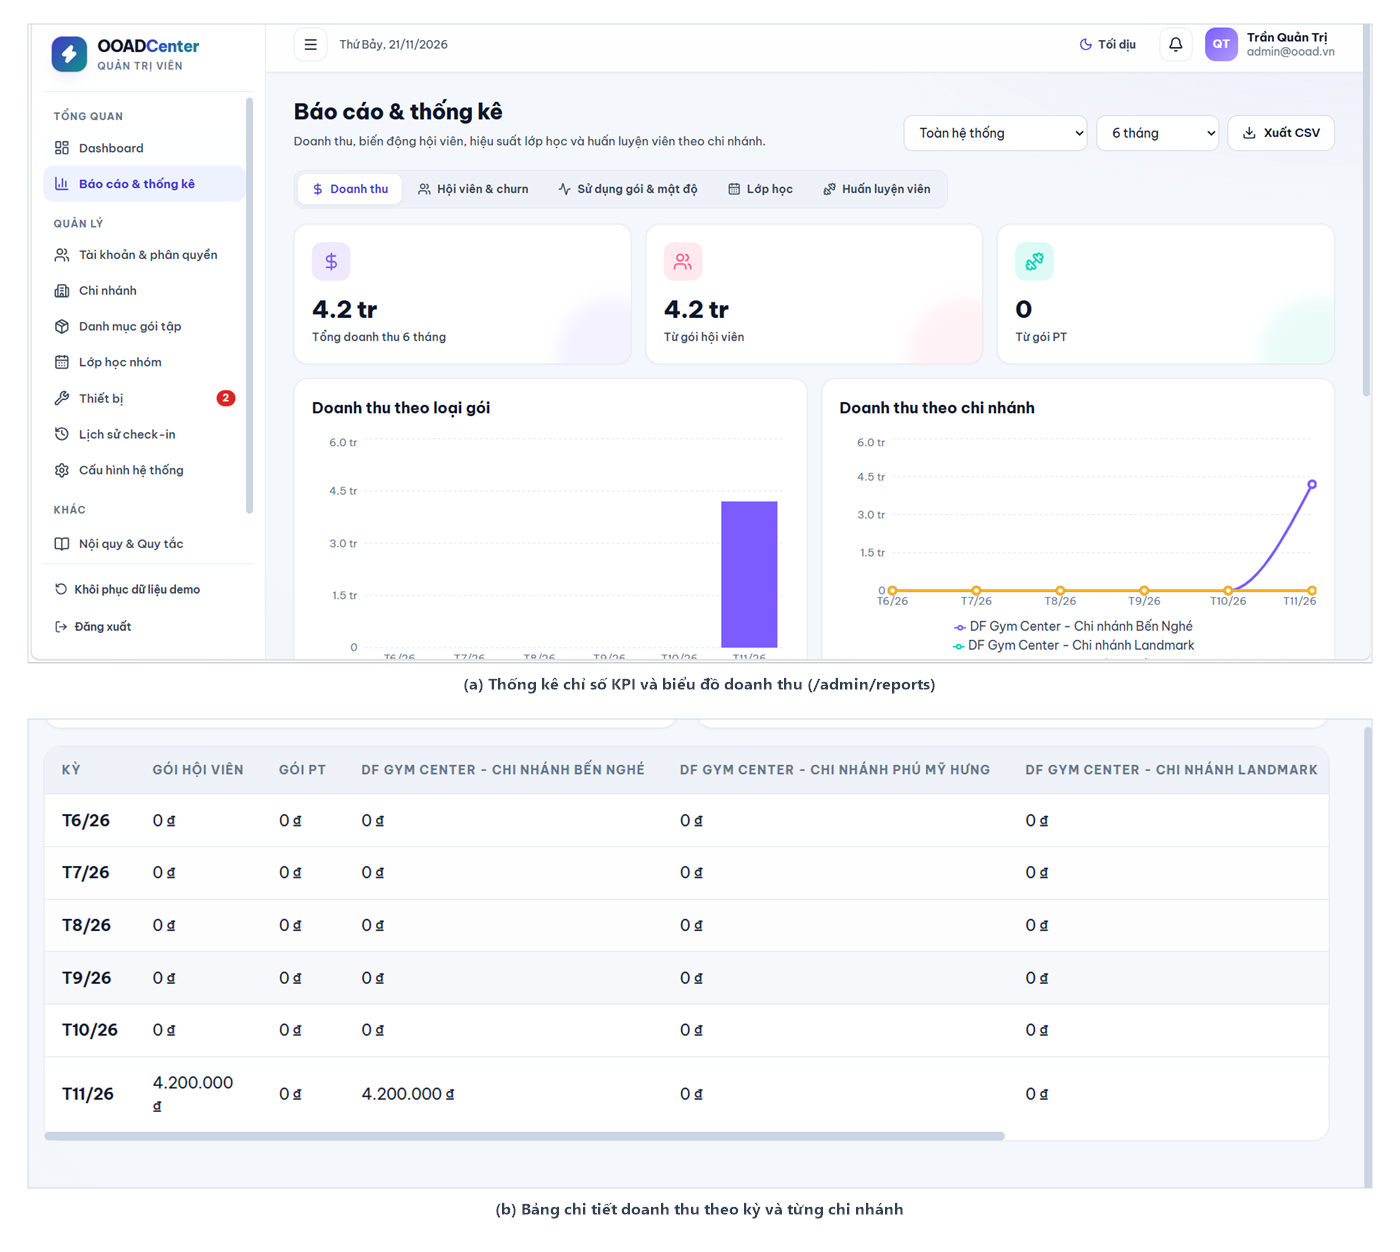
\includegraphics[width=0.92\textwidth]{images/ui_truc/mh10_admin_reports.png}
\caption{Giao diện màn hình Báo cáo và Thống kê Tổng quan}
\label{fig:mh10_admin_reports}
\end{figure}

\par\medskip\noindent\textbf{Danh sách các thành phần giao diện}\par\smallskip
{\footnotesize
\setlength{\tabcolsep}{2.5pt}
\begin{longtable}{|c|L{2.95cm}|L{1.85cm}|L{2.95cm}|L{2.75cm}|L{1.90cm}|L{2.05cm}|}
\hline
\textbf{STT} & \textbf{Tên} & \textbf{Kiểu} & \textbf{Ý nghĩa} & \textbf{Miền giá trị} & \textbf{Giá trị mặc định} & \textbf{Ghi chú} \\
\hline
\endfirsthead
\hline
\textbf{STT} & \textbf{Tên} & \textbf{Kiểu} & \textbf{Ý nghĩa} & \textbf{Miền giá trị} & \textbf{Giá trị mặc định} & \textbf{Ghi chú} \\
\hline
\endhead
\hline
\endfoot
\hline
\caption{Danh sách các thành phần giao diện -- Màn hình Báo cáo và Thống kê Tổng quan} \\
\endlastfoot
1 & \texttt{Cbo\_PhamViCN} & ComboBox & Lọc số liệu báo cáo toàn hệ thống hoặc theo một chi nhánh lẻ & Tất cả / Danh sách từ \texttt{Branches} & \texttt{"Toàn hệ thống"} & Tác động lên toàn bộ KPI và biểu đồ \\ \hline
2 & \texttt{Cbo\_\hspace{0pt}KhoangThoiGian} & ComboBox & Chọn khung thời gian tổng hợp dữ liệu báo cáo & \{\texttt{"3 tháng"}, \texttt{"6 tháng"}, \texttt{"12 tháng"}\} & \texttt{"6 tháng"} & Truyền tham số \texttt{months} lên API \\ \hline
3 & \texttt{Btn\_XuatBaoCao} & Button & Kết xuất số liệu báo cáo đang xem ra tệp tin \texttt{.csv} & Kích hoạt & \texttt{"Xuất CSV"} & Tải trực tiếp tại trình duyệt \\ \hline
4 & \texttt{Tab\_NhomBaoCao} & Tab Group & Chuyển giữa 5 chuyên mục: Doanh thu, Hội viên \& churn, Gói \& mật độ, Lớp học, HLV & $5$ nhóm báo cáo & \texttt{"Doanh thu"} & Mỗi tab có bảng và biểu đồ riêng \\ \hline
5 & \texttt{Card\_KPIDoanhThu} & StatCard & Hiển thị Tổng doanh thu kỳ chọn, Doanh thu gói hội viên và Doanh thu gói PT & Số tiền (VNĐ) & Tổng hợp theo kỳ & Chỉ đọc, định dạng tiền tệ \\ \hline
6 & \texttt{Chart\_DoanhThuGoi} & Chart & Biểu đồ cột trực quan hóa tỷ trọng doanh thu theo từng loại gói tập & Dữ liệu tổng hợp từ API & Kỳ mặc định $6$ tháng & Hỗ trợ tooltip chi tiết \\* \hline
7 & \texttt{Chart\_DoanhThuCN} & Chart & Biểu đồ đường đa chuỗi so sánh tăng trưởng doanh thu theo từng chi nhánh & Chuỗi thời gian theo tháng & Kỳ mặc định $6$ tháng & Phục vụ đánh giá hiệu suất cơ sở \\ \hline
\end{longtable}
}

\par\medskip\noindent\textbf{Danh sách các biến cố}\par\smallskip
{\footnotesize
\setlength{\tabcolsep}{4pt}
\begin{longtable}{|c|L{3.5cm}|L{7.8cm}|L{3.5cm}|}
\hline
\textbf{STT} & \textbf{Điều kiện kích hoạt} & \textbf{Xử lý} & \textbf{Ghi chú} \\
\hline
\endfirsthead
\hline
\textbf{STT} & \textbf{Điều kiện kích hoạt} & \textbf{Xử lý} & \textbf{Ghi chú} \\
\hline
\endhead
\hline
\endfoot
\hline
\caption{Danh sách các biến cố -- Màn hình Báo cáo và Thống kê Tổng quan} \\
\endlastfoot
0 & Khởi động màn hình (\texttt{/admin/reports}) & Gọi API \texttt{GET /api/reports/overview?months=6} kèm JWT quản trị; \texttt{ReportService} tổng hợp số liệu từ CSDL để hiển thị \texttt{Card\_KPIDoanhThu} cùng các biểu đồ \texttt{Chart\_DoanhThuGoi}, \texttt{Chart\_DoanhThuCN}. & Mặc định mở chuyên mục Doanh thu. \\ \hline
1 & Thay đổi lựa chọn trên \texttt{Cbo\_PhamViCN} hoặc \texttt{Cbo\_KhoangThoiGian} & Gửi lại yêu cầu \texttt{GET /api/reports/overview} với các tham số \texttt{branchId} và \texttt{months} mới, cập nhật đồng loạt thẻ KPI, biểu đồ và bảng số liệu chi tiết. & Hiển thị mức $0$ nếu chi nhánh chưa phát sinh giao dịch. \\ \hline
2 & Chuyển chuyên mục trên \texttt{Tab\_NhomBaoCao} & Chuyển vùng nội dung hiển thị sang nhóm báo cáo tương ứng (Hội viên \& churn, Sử dụng gói, Hiệu suất lớp học hoặc Hiệu suất HLV). & Dùng chung bộ lọc chi nhánh và thời gian. \\* \hline
3 & Nhấn nút \texttt{Btn\_XuatBaoCao} (\textit{Xuất CSV}) & Chuyển đổi tập dữ liệu báo cáo đã tải sang định dạng bảng tính CSV tại trình duyệt và tự động tải xuống tệp tin báo cáo. & Chỉ kích hoạt sau khi dữ liệu đã tải xong. \\ \hline
\end{longtable}
}


\newpage
\subsection{Tổng hợp và Đánh giá chất lượng thiết kế giao diện}
\subsubsection{Đánh giá theo nguyên tắc kỹ nghệ phần mềm}
Các màn hình giao diện được xây dựng tuân thủ chặt chẽ nguyên tắc kỹ nghệ phần mềm:
\begin{enumerate}
    \item Phân tầng rõ ràng theo kiến trúc Modular Monolith kết hợp Clean Architecture (Presentation -- Application -- Domain -- Infrastructure) tương ứng với các lớp phân tích BCE.
    \item Đảm bảo trọn vẹn 6 phân hệ nghiệp vụ cốt lõi cho 4 vai trò: xác thực \& hồ sơ, gói tập \& thanh toán/Freeze, lớp học nhóm \& Waitlist, đặt lịch PT \& theo dõi chỉ số InBody, check-in \& thẻ hội viên, quản lý thiết bị \& báo cáo thống kê.
    \item Xử lý ngoại lệ đầy đủ ở cả 2 đầu: Client-side validation (phản hồi tức thì) và Server-side business exception handling (bảo đảm an toàn dữ liệu).
\end{enumerate}

\subsubsection{Đánh giá sự tuân thủ các tiêu chuẩn chất lượng giao diện}
\begin{enumerate}
    \item \textbf{Nguyên tắc Tự động tính toán:} 
    Hệ thống tự động phát hiện hạn gói cũ để tính hạn nối tiếp chính xác đến từng ngày; tự động chia trung bình đơn giá mỗi tháng/mỗi buổi PT; tự động cộng bù chính xác số ngày tạm ngưng vào ngày hết hạn mới.
    \item \textbf{Nguyên tắc Phòng ngừa sai sót \& Cảnh báo:}
    Cảnh báo trực tiếp cho lễ tân số lượng lịch đặt sẽ tự động hủy (ví dụ: \textit{``6 lịch sẽ tự hủy''}) trước khi duyệt freeze, tránh tình trạng xung đột thời khóa biểu và lãng phí tài nguyên phòng tập.
    \item \textbf{Nguyên tắc Nhất quán và Công thái học:}
    Toàn bộ hệ thống tuân thủ phong cách thiết kế hiện đại (Modern Clean Flat UI), font chữ rõ nét, màu sắc chuẩn hóa mang tính định hướng cao (Xanh lá = An toàn/Hiệu lực, Xanh tím = Hành động chính, Cam = Cảnh báo/Chờ duyệt, Đỏ = Từ chối/Thất bại).
    \item \textbf{Độc lập giữa Giao diện và Xử lý:}
    Giao diện Presentation Layer chỉ đảm nhận việc thu nhận biến cố và hiển thị kết quả, toàn bộ nghiệp vụ kiểm tra Quota, bù ngày và tạo hóa đơn được xử lý tại Application Layer và Domain Layer, giúp hệ thống dễ dàng bảo trì, mở rộng và tiến hóa lâu dài.
\end{enumerate}


% ==============================================================================
% 7. KẾT LUẬN
% ==============================================================================
\newpage
\section{Kết luận}
\textit{(Hiện tại chưa làm, nội dung tổng kết và hướng phát triển sẽ được bổ sung sau khi hoàn thiện hệ thống.)}

\end{document}
